\documentclass[leqno]{surv-l}


\usepackage{amssymb,graphicx}
\usepackage[mathscr]{euscript}
\usepackage{amsmidx}
\usepackage[noadjust]{cite}

\newtheorem{theorem}{\sc Theorem}[section]
\newtheorem{exercise}{\sc Exercise}[section]
\newtheorem{lemma}{\sc Lemma}[section]
\newtheorem{corollary}{\sc Corollary}[section]
\newtheorem{proposition}{\sc Proposition}[section]
\newtheorem{lemma1}[theorem]{\sc Lemma}
\newcommand\circledinfty{\ooalign{$\bigcirc$\cr$\infty$\cr}\space}
\newenvironment{copyrightpage}{\clearpage\null\thispagestyle{empty}}{\thispagestyle{empty}\clearpage}


\theoremstyle{definition}
\newtheorem{definition}{\sc Definition}[section]
\newtheorem*{proof*}{\sc Proof}
\newtheorem*{proof1*}{\emph{Proof}}
\newtheorem{example}{\sc Example}[section]
\newtheorem{step}{Step}
\newtheorem{remark}{\sc Remark}[section]
\newtheorem*{remark*}{Remark}
\newtheorem{application}{Application}
\newtheorem{assumption}{\sc Assumption}[section]
\newtheorem{definition1}[theorem]{\sc Definition}
\newtheorem{remark1}[theorem]{\sc Remark}
\newtheorem{corollary1}[theorem]{\sc Corollary}

\numberwithin{equation}{section}


\makeindex{symbols}

\makeindex{index}


\begin{document}

\begin{titlepage}
Stochastic Partial Differential Equations: Six Perspectives
\end{titlepage}

\title{Stochastic Partial Differential Equations: Six Perspectives}

\author{Rene A. Carmona}

\author{Boris Rozovskii}

\author{Editors}

\maketitle

\begin{copyrightpage}
\begin{center}
\textbf{Editorial Board}\\
Georgia M. Benkart \qquad  Tudor Stefan Ratiu, Chair\\
Peter Landweber \qquad\quad\ Michael Renardy
\end{center}

\begin{center}
1991 \emph{Mathematics Subject Classification}. Primary 60H15; Secondary 35R60.
\end{center}

\noindent \textsc{Abstract.} Stochastic Partial Differential Equations is an interdisciplinary area on the crossroads of stochastic processes (random fields) and partial differential equations. This volume presents the topic of SPDE's from different perspectives, as seen by six groups of researchers working in the most active and promising areas of the field. The goal of this book is to indicate what the main topics of interest are in this fascinating field, and where breakthroughs are being made today.

This book will be of interest to graduate students and researchers in various areas of Mathematics, Physics, Engineering, Economics, etc.\\

\hrulefill\\

\noindent \textbf{Library of Congress Cataloging-in-Publication Data}

\noindent Stochastic partial differential equations : six perspectives / Rene A. Carmona, Boris Rozovskii, editors.

\quad p.cm. --- (Mathematical surveys and monographs, ISSN 0076-5376 ; v. 64)

Includes bibliographical references (p. - )and index.

ISBN 0-8218-0806-0 (alk. paper)

1. Stochastic partial differential equations. I. Carmona, R. (Ren\'{e}) II. Rozovski\u{\i}, B. L. (Boris L$^{\prime}$vovich) III. Series: Mathematical surveys and monographs ; no. 64.

\noindent QA274.25.S746 \quad  1998

\noindent 519.2---dc2l \hfill 98-38392

\hfill CIP\\

\hrulefill\\

\noindent \textbf{Copying and reprinting.} Material in this book may be reproduced by any means for educational and scientific purposes without fee or permission with the exception of reproduction by services that collect fees for delivery of documents and provided that the customary acknowledgment of the source is given. This consent does not extend to other kinds of copying for general distribution, for advertising or promotional purposes, or for resale. Requests for permission for commercial use of material should be addressed to the Assistant to the Publisher, American Mathematical Society, P. O. Box 6248, Providence, Rhode Island 02940-6248. Requests can also be made by e-mail to \textbf{\texttt{reprint-permission@ams.org}}.

Excluded from these provisions is material in articles for which the author holds copyright. In such cases, requests for permission to use or reprint should be addressed directly to the author(s). (Copyright ownership is indicated in the notice in the lower right-hand corner of the first page of each article.)

\begin{center}
$\copyright$ 1999 by the American Mathematical Society. All rights reserved.\\
The American Mathematical Society retains all rights\\
except those granted to the United States Government.\\
Printed in the United States of America.
\end{center}

\begin{center}
$\circledinfty$\ The paper used in this book is acid-free and falls within the guidelines\\
established to ensure permanence and durability.\\
Visit the AMS home page at \textbf{URL: \texttt{http://www.ams.org/}}
\end{center}

\begin{center}
10 9 8 7 6 5 4 3 2 \qquad 04 03 02 01 00 99
\end{center}
\end{copyrightpage}

\frontmatter

\tableofcontents

\chapter*{Preface}

This volume is an attempt to present the topic of Stochastic Partial Differential Equations (SPDE's) from different perspectives, as seen by six groups of researchers working in the most active and promising areas of the field.

As the name suggests, Stochastic Partial Differential Equations is an interdisciplinary area at the crossroads of stochastic processes (random fields) and partial differential equations. Interacting particle systems, nonlinear filtering, super processes, continuum physics, $\ldots$ have heavily influenced the development of SPDE's. It is safe to say that in the last two decades SPDE's has been one of the most dynamic areas of stochastic processes. Stochastic effects are of central importance for the development of mathematical models of many phenomena in physics, biology, economics, $\ldots$ . However, most often the resulting (limiting) models end up being deterministic. (Many classes of particle systems and their hydrodynamic limits provide good examples of this effect.) These models usually result from the law of large number type of averaging and they represent the large scale \emph{mean} dynamics of the modeled phenomena. The predictive power of such models might be limited especially for very complex phenomena such as turbulence, phase transition, dynamic instability, chaos, $\ldots$ . In these and some other situations, stochastic corrections to the deterministic large scale models are very much in order. These corrections are designed to account for the small scales effects neglected in the large scale models. One heuristic way to incorporate these corrections is to perturb the large scale equation by random noise of some kind. Sometimes the stochastic corrections can be derived rigorously by a type of renormalization/central limit theorem of fluctuations around stable large scale models. In fact, in many applications the derivation of the \emph{right} stochastic corrections to the large scale dynamics and their practical utility present one of the fundamental challenges.

Generally speaking, any partial differential equation should be classified as an SPDE if its coefficients, forcing terms, initial and boundary conditions, or at least some of the above are random. Needless to say, this constitutes an extremely diverse area. For example, the analysis of equations with random coefficients has little in common with the analysis of deterministic equations with random free forces. As typical of research fields in their early stages of development, the paradigm of SPDE's is still fairly \emph{soft:} the name SPDE covers different topics for different people. As of now, the subject of SPDE's with its numerous important applications is an exciting mosaic of interconnected topics revolving around stochastics and partial differential equations. It is arguable whether a single book could or should treat the enormously complex field of SPDE's from a unified point of view and this is not the goal of this book. The goal of this book is to indicate what the main topics of interest in this fascinating field are, and where breakthroughs are being made today. As much as emphasizing breakthroughs however, we tried to explore the role of SPDE's in stochastic modeling, how SPDE's arise and how their theory is applied in different disciplines.

The book is divided into two parts. Part I, \emph{SPDE's and Stochastic Modeling}, deals with fundamental problems in continuum physics, fluid dynamics, statistical mechanics, and branching particle systems and geneses of various types of SPDE's in these fields. Part II, \emph{Mathematical Theory of SPDE's}, is concerned with methods of solutions and related stochastic analysis. Every chapter of the book presents a comparatively self-contained review of a particular sub-field of SPDE's or a related area. Many new previously unpublished results are included as well. Part I consists of four chapters. Chapter~\ref{ch01:chap01} emphasizes the conceptual basis for stochastic modeling and more specifically, modeling with SPDE's. This chapter also investigates the relations between stochastic and deterministic models in continuum physics. It should provide the reader with a considerable insight of the role of SPDE's in modeling of physical phenomena. Chapter~\ref{ch02:chap02} deals with the asymptotic renormalization of systems of particles undergoing branching and spatial motion and some classes of measure-valued processes, which arise in the limit. The small scale and large scale behavior of these systems are described and various generalizations and extensions of these models which include interactions both between particles and between particles and the medium in which they live are surveyed. Chapter~\ref{ch03:chap03} addresses deterministic and stochastic hydrodynamic equations arising from microscopic model systems. Physical and mathematical aspects of stochastic corrections to the hydrodynamic scaling limit for various important types of interacting particle systems are discussed in this chapter. Chapter~\ref{ch04:chap04} is devoted to transport of passive scalars by 2D incompressible random velocity fields. The chapter pays special attention to stochastic numerics. Numerical simulations are used both to illustrate the relevance of the theoretical results and to formulate new conjectures, some of them proved later on. Chapter~\ref{ch05:chap05} and~\ref{ch06:chap06} constitute the second part of the book. Chapter~\ref{ch05:chap05} is devoted to linear and some quasi-linear parabolic SPDE's. Equations of this type arise for example in nonlinear filtering of diffusion processes, the problem that was one of the most important original impetuses for the development of SPDE's. This chapter presents a detailed exposition of recent advances in solvability of these equations in Sobolev spaces and spaces of Bessel potentials with exponent of summability greater than or equal to 2. Chapter~\ref{ch06:chap06} is concerned with nonlinear stochastic PDE's with nonsmooth (in some cases singular) coefficients. The examples include stochastic Navier-Stokes equation, Langevin (stochastic quantization) equation in Euclidean quantum field theory, SPDE's for the super-Brownian motion and some related super processes. The emphasis in this chapter is on existence and uniqueness of weak solutions, absolute continuity and singularity of distributions, and ergodicity problems for these equations.

Of course, this book could not possibly cover all or even most of the important developments and problems of SPDE's. However, we believe that it will provide the interested reader an informative snapshot of this rapidly developing area. The idea of the book was conceived at the Workshop on Stochastic Partial Differential Equations held at the University of Southern California, Los Angeles, in January of 1996. In more than one way the discussions and the lectures at the Workshop prompted this book.\\

\noindent \emph{Acknowledgments}

As the editors of this volume and the organizers of the Workshop, we would like to take this opportunity to acknowledge the support of the Army Research Office, the Office of Naval Research, and the Institute for Mathematics and Its Applications. Our thanks are due to Patricia Shapiro for the help in editing this volume. Finally, we would like to thank the AMS staff for their cooperation and patience. The contribution of J. Glimm was partially supported by the Applied Mathematics Subprogram of the U.S. Department of Energy DE-FG02-90ER25084, the Army Research Office, grant DAAL03-92-G-0l85 and the National Science Foundation, grant DMS-9500568 while D. Sharp was supported by the U.S. Department of Energy. Both D. Dawson and E. Perkins would like to acknowledge the support of NSERC of Canada Research Grants and of a joint NSERC of Canada Collaborative Grant. During the preparation of their manuscript, G. Giacomin was partially supported by the Swiss National Foundation project 20-41'925.94, the IHES and Rutgers University, while J. L. Lebowitz was partially supported by AFOSR grant 92-J0115, NSF grant DMR-95-23266 and the IHES and E. Presutti was partially supported by CEE grant CHRX. CT93-0411, the Courant Institute and Rutgers University. R. A. Carmona's contribution was supported in part by ONR grant \# ONR N00014-91-1010. N.V. Krylov's work was partially supported by the NSF Grant DMS-9625483. Finally, B. Rozovskii and M. Mikulevicius were supported by ONR Grant N00014-95-1-0229 and ARO Grant DAAH04-95-1-0164.\\

\hfill RENE A. CARMONA

\hfill Statistics \& Operations Research, C.E.O.R.

\hfill Princeton University

\hfill Princeton, N.J. 08544\\\\

\hfill BORIS ROZOVSKII

\hfill Center for Applied Mathematics Sciences

\hfill University of Southern California

\hfill Los Angeles, CA 90089-1113\\

\hfill March, 1998

\mainmatter


\part{STOCHASTIC MODELS\label{pt01:part01}}

%%%%%%%%%%%chapter01

\chapter{Stochastic Partial Differential Equations: Selected Applications in Continuum Physics \label{ch01:chap01}}


\hfill JAMES GLIMM

\hfill SUNY at Stony Brook

\hfill Stony Brook, NY 11794-3600

\hfill \texttt{glimm@ams.sunysb.edu}\\


\hfill DAVID SHARP

\hfill The Los Alamos National Laboratory

\hfill Los Alamos, NM 87545

\hfill \texttt{dhs@t13.lanl.gov}\\

\section{The Physical Basis of Stochastic Analysis}
\label{ch01:sec1}

Stochastic modeling occupies a central place in the derivation of
the equations of continuum physics. This fact is obscured by another
fact: the desired outcome of this modeling is often a deterministic
partial differential equation. Thus the stochastic model may be
important either as an intermediate step towards a deterministic
theory, or as a final theory in its own right. As we move toward a
more realistic acceptance of probability as an essential component
in the analysis of complex phenomena, the role of a stochastic model
as a final outcome of the analysis will increase. This trend is
illustrated, for example, by probabilistic weather
forecasts\index{index}{weather!forecasts} \cite{ch01:bib23,
ch01:bib58}, probabilistic simulation studies to support petroleum
reservoir\index{index}{petroleum reservoir} management decisions
\cite{ch01:bib81, ch01:bib31} and probabilistic financial decision
making\index{index}{financial decision making} \cite{ch01:bib102,
ch01:bib103}. As we demand increased accuracy and reliability from
our deterministic models, the need to examine their stochastic
components and derivations will also increase. For both reasons, we
see a need to emphasize the importance of stochastic models of
physical systems.

Stochasticity in models of physics arises from several sources. A principal factor leading to stochasticity is dynamical instability and sensitive dependence on initial conditions, in a microscopic dynamics which can be deterministic in principle. Closely related to this factor is the absence of sufficient deterministic data to specify a solution of the governing equations. In a probabilistic approach, such input data is supplied statistically, which leads to a statistical version of the final answer. The deterministic laws of physics cannot be ignored in this procedure, so that the model will be stochastic, and not purely statistical. Moreover, partial information cannot be ignored, so that the probability measures will be conditioned by partial knowledge. Finally, in some cases a complete deterministic model of a system may be lacking, owing to missing science.

This chapter begins with a discussion of the basic ideas underlying stochastic modeling in continuum physics, followed by a brief overview of selected areas where such modeling is playing an important role. In these examples, the governing equations are usually the partial differential equations of classical physics. We next review methods that are under development for stochastic analysis in this context. The application of these methods is illustrated in discussions of multi-phase flow in chaotic mixing layers and of the transport and dispersion for flow in porous media. The scientific issues raised in this chapter are ones which, in the authors' judgment, deserve deeper examination.

\subsection{The Conceptual Framework}
\label{ch01:sec1.1}

Stochastic phenomena, such as ``noise'', commonly arise in models of physical systems. Models are generally an incomplete description of nature, and noise represents some of the effects present in nature, but missing from the model.

Noise may refer to effects omitted from a model due to lack of data but often, and more fundamentally, noise refers to a loss of predictability. This typically occurs when the physical process being modeled is unstable, in which case a deterministic solution will depend sensitively on the problem data. Even minute variations in the data (such as the initial conditions, the physical parameters which occur in the defining equations, or even the functional form of the equations) can yield large variations in the solutions. In such cases deterministic prediction requires unreasonably large amounts of data, so that in a practical sense, there can never be enough data to predict the solution. Moreover, even if sufficient data were available, numerical solution methods with finite accuracy of time step integration and finite accuracy arithmetic do not generally produce stable, reliable solutions and even if they do, they cannot do so in an efficient, cost effective manner. Thus, viewed deterministically, a problem may be unsolvable, or highly intractable. It is in this sense that while lack of data may be seen as the requirement which forces the use of stochastic modeling, the more fundamental cause is lack of stability or sensitive dependence on data.

Stochastic modeling succeeds when the statistical formulations are predictive. This occurs when the mapping from stochastically specified data to a stochastically specified solution is well conditioned, so that it does not suffer from sensitive dependence on its data. It can very well be the case that the stochastic formulation is predictive, even when the deterministic formulation is not. However, in this case one has to settle for less detailed information, such as stochastic averages or moments, than would be present in the deterministic solution. For example, one might be able to predict the probability of rain tomorrow, rather than its certain occurrence.

Thus ``noise'' is not just an irritating detail, introduced to compensate for defects in a deterministic model, but is rather an intrinsic phenomenon for which a probabilistic description succeeds while a deterministic one fails. An example is the toss of a coin. A skilled performer can flip coins deterministically, and systematically produce heads or tails as desired \cite{ch01:bib28}. But lacking such skill, concentration, and training, the common probability model is more satisfactory as a description of the event than would be a deterministic description based on forces imparted to the coin, the difference in height between the point where the coin is tossed and the point where it is caught, and its mass and moment of inertia.

For the purposes of the present discussion, we define our model by a partial differential equation, either in conservation form,
\begin{equation}
\label{ch01:eqn1.1} U_{t}+\nabla F(U)=0,
\end{equation}
or in conservation-diffusion form,
\begin{equation}
\label{ch01:eqn1.2} U_{t}+\nabla F(U)=\nabla \nu\nabla U.
\end{equation}
Here $U=U(x,\,t)=U(x,\,t,\,\omega)$ is the solution. In the deterministic case the dependence on $\omega$ is missing, while in the stochastic case, $\omega \in\Omega$, with $\Omega$ a measure space. Then $U$ is a random variable or, more properly, a random field\index{index}{random!field}, because it depends on multiple independent variables, $x,\,t$. $U$ is random either because its data is random, or because of random terms in the equation itself. Thus the initial data, $U(x, t=0)$ may be random, so that $U(x, t=0)=U(x, t, \omega)|_{t=0},\,w \in\Omega$, or the boundary data (not shown above) may be random. Randomness in the equation can occur if, for example, the flux function $F=F(U)=F(U, x, t, \omega)$, is random or if the diffusion coefficient $\nu$ is random. In view of the above discussion, we regard $U$ as stochastic when it has sensitive dependence on the problem data.

We emphasize the use of random fields to represent noise in partial differential equations. A partial differential differential equation is an infinite system. Its data belongs to an infinite dimensional function space. The solution correspondingly possesses an infinite number of degrees of freedom. Potentially the noise does also.

There are situations in which only a few of these infinitely many degrees of freedom are unstable. In this case the deterministic system is infinite dimensional but the noise (at each instant of time) is finite dimensional. Such a system displays finite dimensional chaos. The stochastic description, if there is one, is given by a stochastic process, where the random function $\omega(t)$ takes its values in a finite dimensional space, such as the subspace of instability or chaos in the solutions of the partial differential equation. Simple models of atmospheric motion, obtained by truncating the Oberbeck
- Boussinesq equations for fluid convection in a heated two-dimensional layer, lead to a set of low order ordinary differential equations, known as the Lorenz equations\index{index}{Lorenz equations} \cite{ch01:bib71}, whose solutions exhibit a strange attractor in the long time asymptotic limit. A measure on this strange attractor would be a probabilistic description of the chaotic, or deterministically unpredictable, solutions of the Lorenz system, or of this portion of the solution of the original partial differential equation.

Such a situation may be relevant to climatology. Climatology attempts to predict long term trends in the weather\index{index}{weather}, using the same equations and computer simulation programs (known as the general circulation model) which are used to predict the weather. Current accuracy for weather predictions from these models is on the order of five days. In order to assess such questions as global warming or ozone depletion, predictions for years or hundreds of years are needed. Obviously the climatology predictions suffer from a sensitive dependence on data, and thus must be stochastic in nature. In fact, stated conclusions from these models, such as average annual temperature, are stochastic in nature, because of the large degree of averaging contained in this form of the answer. To some extent, there are or may be a moderate or small number of degrees of freedom in the atmosphere which largely govern such averaged predictions. For example the El Ni\~{n}o ocean current is believed to influence rainfall patterns over a large portion of the globe. In an atmospheric model (with no ocean coupling), El Ni\~{n}o would be modeled by stochastic boundary data, and the resulting rainfall statistics would be a stochastic aspect of the solution, with both of these features modeled in finite dimensional subspaces of the data and solutions.

We are interested here in the opposite situation, in which there is a very large, or effectively infinite, number of unstable degrees of freedom which participate actively in determining the solution. Commonly, and as we assume here, the infinite number of degrees of freedom arise from a finite or possibly infinite number of degrees of freedom in each finite spatial domain. In other words, we assume an infinite domain for our partial differential equation, and spatially distributed and localized noise over this infinite domain. In this situation, both the noise and the solutions must be modeled as random fields. In some examples, such as infinite Reynolds number turbulence\index{index}{turbulence}, or as an approximation to finite but large Reynolds number turbulence, we encounter an infinite number of unstable modes in a finite volume. Physically this simply means that more, or all, of the available problem degrees of freedom have become unstable. Fully developed turbulence is such a problem.

According to this discussion, we now assume that the measure space $\Omega$ is built on a function space, i.e. a space of functions of space or space and time, and that a measure $d\omega$ is defined on this space. In accordance with the probabilistic interpretation of the measure, we assume that the total measure of $\Omega$ is 1, so that $\int_{\Omega}d\omega =1$. For each $\omega \in\Omega$, the corresponding (deterministic) functions, \emph{e.g}., $x,\,t\rightarrow U(x, t, \omega)$ or $U,\,x,\,t, \rightarrow F(U, x, t, w)$, are called a \emph{realization} of the random fields $U$ or $F$. It is logically correct, and conceptually clearer to suppress $\omega$ entirely, and just say that $U\in\Omega$, where $\Omega$ is a suitable function space having a distinguished probability measure. Having done this, we will replace $\Omega$ with an alternate notation also.

Using the measure $d\omega$, we define averaged field quantities $\bar{U}=\int_{\Omega}U\,d\omega$, and in a mathematically exact manner, derive an averaged equation, such as
\begin{equation}
\label{ch01:eqn1.3} \bar{U}_{t}+\nabla\bar{F}(U)=0.
\end{equation}
Because of the nonlinearity, $\bar{F}(U)\neq F(\bar{U})$. The averaged equation does not close, because it contains the unknown quantity $\bar{F}(U)$. Closure\index{index}{closure} is the step in which $\bar{F}$ is replaced by some known quantity. It is thus the process of defining the otherwise undefined averages of products or other nonlinear expressions in terms of known quantities, such as products (or some other function) of the averages. These relations are not derived mathematically as a deterministic identity, but rather reflect a statement concerning typical, or average, configurations of the stochastic degrees of freedom. In this sense, closure is very much akin to determination of the equation of state from the statistics of likely particle configurations in a gas. The equations which result from closure are called \emph{effective} equations\index{index}{effective equation}.

Effective equations are the final step in the stochastic modeling process. With these equations, we have gone from a deterministic but unstable equation, to a stochastic model and stochastic partial differential equation, to the solution of the stochastic aspects of this equation, and back to a new deterministic equation. The final equation, even if it has the same form as the original, has a very different interpretation, and generally very different physical parameters. Small length scales have been integrated out in the solution, and the equation now refers to quantities defined on a larger (macro) scale.

The simplest way to obtain a stochastic partial differential equation is to add a Wiener measure term $d\mu$ or white noise to a deterministic partial differential equation. Starting with 1.1, we thus obtain
\begin{equation}
\label{ch01:eqn1.4} U_{t}+\nabla F(U)=d\mu.
\end{equation}
Assuming that $U$ approaches a constant at infinity, so that there is no net flux coming in from infinity, 1.1 implies that $\int_{R^{n}}U\,dx$ is time independent, \emph{i.e}., conserved. Components of $U$ represent quantities such as mass and momenta, which must be conserved in an isolated system, according to basic laws of physics. Additive noise, as in 1.4, models the incomplete isolation of a subsystem from some larger universe, and the coupling between the two typically represents the transfer of mass, momentum, \emph{etc}. into the subsystem. While this type of random additive coupling is of interest, we emphasize the randomness introduced above from the problem data ($U(x, t=0)$ and $F$), involving random fields\index{index}{random!field} rather than random processes, as being more typical of applications. Moreover, the correlation structure of the noise or data, which has a significant effect on the stochastic nature of the solution $U$, is not arbitrary. It is dictated by the application, and is generally not given by Wiener measure or white noise. Finally, we note that the random field is usually not Gaussian, or equivalent to Gaussian, for nonlinear problems. For these reasons, we do not consider 1.4 further.

\subsection{Examples}\label{ch01:sec1.2}

We next discuss examples which illustrate, to varying degrees, the conceptual framework presented above. The examples are drawn from the physics of continuum systems, and are also selected for their current interest.

\textbf{Brownian Motion and the Diffusion Equation}. This example is familiar and highly developed. For this reason, our discussion will be brief. A small particle is suspended in a fluid and subject to random collisions with fluid particles. Each collision results in a random displacement of the particle, which thus executes the (mathematically defined model of) Brownian motion. In a continuum limit of infinitesimal waiting times between collisions and infinitesimal collision displacement steps, this process is the Wiener process. Upon averaging, or through consideration of expected values, the Wiener process yields the solution of the diffusion equation, a deterministic partial differential equation, which is the effective equation, in the terminology of \S 1.1.

The same modeling process applies to a number of other physical situations, such as heat conduction, and the dispersion of fluid flow through a heterogeneous medium.

\textbf{Statistical Physics and the Equation of State}\index{index}{equation of state}. This is also a mature example. Molecules move according to Newton's laws, in response to intermolecular forces. Since the number of molecules, on the order of Avogadro's number, $10^{23}$, is very large, the state space for this system is approximately infinite dimensional. (We leave it as an exercise to the mathematically minded to determine which finite numbers are approximately infinite and which are not.) Individual values of all the molecular coordinates and momenta are not available as initial data in a practical sense, and their evolution under Newton's equations depends sensitively on this data. Thus we need a stochastic description, which is given by the theories of statistical physics \cite{ch01:bib59}. Various equilibrium ensembles correspond to different methods of conditioning the system, \emph{i.e}., of specifying the allowed system states and the measure on the space of states. Averaging the equations of motion relative to suitable measures over this state space defines the moment equations of kinetic theory, such as the Boltzmann equation. A further asymptotic limit, in which the probability distribution for the velocity is replaced by its low order moments, leads to the Euler and Navier-Stokes equations for fluid flow. The fluid equations must be supplemented with a statistically defined equation of state\index{index}{equation of state} which, for example, expresses the total system energy as a function of other averaged variables, such as density and entropy. The determination of the functional form of the system energy is an example of the closure problem, to be discussed in more detail below. The solution to this problem is also determined in principle by a suitable averaging procedure, which leads to equations of state whose study is the subject of thermodynamics. This well developed example illustrates the statistical issues associated with closure\index{index}{closure}, and provides guidance for the analysis of closure problems in other contexts.

Computational evaluation of the equation of state comes from a computational solution of the statistical physics problem. There are a number of open problems, both theoretical and computational, in connecting the statistical physics model to the thermodynamics, \emph{i.e}., the equation of state.

We have seen that stochastic modeling connects unstable microscopic deterministic equations (Newton's equations for a large number of particles) with macroscopic deterministic equations (\emph{e.g}., the Euler equations). As discussed below, the macroscopic flow equations themselves may or may not be unstable and thus may, depending on the flow regime, require another level of stochastic modeling, to yield a new deterministic averaged equation.

It is a characteristic feature of the modeling of natural phenomena that distinct models are needed on distinct length scales, and that phenomena which are deterministic on one scale may be stochastic on another, to be averaged out. The equations, as one passes from smaller to larger length scales, may change their form, and even when they do not, the physical parameters within the equations may change their values. The integration of small length scales to obtain new equations which govern only the large length scale phenomena is called \emph{renormalization}\index{index}{renormalization}. In some cases, the integration steps to larger length scales can be carried out in a continuous, rather than discrete, fashion. In this case, the equations change continuously, and perhaps even differentiably, with the change of length scale $l$, leading to a differential equation for equations (or the parameters in them) of the symbolic form
\begin{equation}
\label{ch01:eqn1.5} \frac{d(\mathrm{Equation})}{dl}+\beta(\mathrm{Equation})=0.
\end{equation}
for some functional $\beta$. See Section~\ref{ch01:sec2.3} for further discussion.

\textbf{Dislocations\index{index}{dislocation}, Burger's Vectors\index{index}{Burgers vector} and Constitutive Laws}\index{index}{constitutive laws}. Most solids are not perfect crystals. For example, common metals are polycrystals, made up of microscopic crystalline domains, joined along walls which represent defects in the crystalline structure. Additional crystal defects occur along dislocation lines, and as point defects, such as impurities, voids and inclusions. The statistical distribution of the defects and impurities is very important, as it determines the properties of the polycrystalline material. These properties are very different from those of the pure crystal. The line defects occur at the edge of an extra half plane of lattice sites inserted into the lattice. Their motion through the lattice is associated with plastic deformation. A continuum model of the line defects in a lattice is a curve, with a tangent known as a Burger's vector. When these are considered statistically and averaged, a density of Burger's vector fields (line defects) \cite{ch01:bib64} results. A further integration of the continuum level defect models leads to stress-strain laws, \emph{i.e}., constitutive laws for the solid, including plastic yield. These laws are just the equation of state (and possibly its non-equilibrium extension) encountered above for fluids, but now in the context of solid materials. Thus we see that material properties are defined by phenomena at several different length scales. In principle, behavior on one length scale is determined from a stochastic model of defects on a smaller one. But the practical solution of these stochastic models to give their coupling across length scales still presents many difficulties. In summary, we view the equations for the flow of solid materials, such as those describing elasto-plastic deformations, as resulting from the integration of stochastic models describing phenomena on smaller length scales, starting from the atomic scale. To fully implement this vision is a major challenge to contemporary science.

\textbf{Material Damage Models, Shear Bands\index{index}{shear!band}, Voids, and Fracture}\index{index}{fracture}. Here we start with the continuum equations of, for example, an elasto-plastic material. These materials support several types of failure modes. Shear bands result from a thermal instability: Laminar shearing is unstable to highly localized shearing, since shearing induces heat, which softens the material, allowing a further (and localized) concentration of the shear stress. Voids and fracture result from a breaking of lattice bonds. The one sided damage to the material at a fracture tip results in a concentration of stress at that location, again giving rise to an instability. In some regimes, there is a profusion of micro-fractures, or of shear bands, or of voids. In such cases, these features must be treated stochastically. The deterministic continuum equations have effectively stochastic solutions. An averaging procedure will lump the combined effects of many micro-voids, bands, or fractures into a type of average material property for the partially damaged material. These averaged properties appear in averaged equations, and describe in a deterministic fashion the stochastic aspects of the ensemble of micro-voids, bands and fractures. However, there are again many difficulties -- theoretical, practical, and computational -- in implementing this program, and it is far from a completed body of science.

\textbf{Multi-phase Flow}\index{index}{multi-phase flow}. When two fluids mix at a molecular level, they behave as a single fluid, but with a modified equation of state which describes the single fluid resulting from the mixture. Multi-phase flow refers to any other type of mixing, \emph{i.e}., mixing which does not occur at the molecular level, but rather in terms of droplets, slugs, \emph{etc}. of one fluid mixed into the other. At a microscopic level the flow is modeled by the Euler or Navier-Stokes equations applied to each fluid individually with an interface, moving with the local fluid velocity, to separate them. There are many distinct flow regimes in which this mixing can occur, each having distinct behavior. Spray or mist consists of small droplets of heavy fluid mixed into an ambient lighter fluid. A bubbly fluid describes the opposite situation of small bubbles of light fluid interspersed in an ambient heavy fluid. Slug flow describes a situation in which the droplets are larger, on the order of the length scale characterizing the flow itself; for example the pipe diameter, for flow in a pipe. Further complications arise from mass transfer between fluid components, as in the case of partial solubility of one component in another, or in the case of phase transitions. These flow configurations are unstable in the sense of \S 1.1, and the microscopic equations are not suitable for prediction. The microscopic equations are regarded as random, and after averaging \cite{ch01:bib29, ch01:bib30}, a new set of deterministic equations are introduced. These equations describe average quantities such as the local average bubble or droplet concentration, considered as new system dependent variables, and represented as functions of space and time. Multi-phase flow\index{index}{multi-phase flow} is important in such applications as fuel injection in diesel and automotive engines, pipeline flow, and the design of chemical reactors.

\textbf{Turbulence}\index{index}{turbulence}. Turbulence is the phenomenon of instability and loss of predictability for flows described by the Navier-Stokes equation. It is characterized by flows with a large Reynolds number $R$, where $R=vL/\nu$ with $v$ the velocity, $L$ a typical system length scale, and $\nu$ the viscosity. At small length scales on the order of $l_{\mathrm{visc}}=\nu/v$ the effective Reynolds number is 1, and the flow is laminar (\emph{i.e}., stable, and with a smooth dependence on flow data). This length scale is called the dissipation length. At this length scale, dissipation effects dominate, and energy is rapidly converted into heat. At length scales comparable to $L$, the flow is dominated by system dependent features, \emph{e.g}., large vortices in the flow pattern. Thus neither the small nor the large length scales should be considered to be stochastic.

Kolmogorov\index{index}{Kolmogorov} proposed that for length scales in the range $l_{\mathrm{visc}}\ll l\ll L$, called the inertial range, turbulence is universal, \emph{i.e}., independent of the Reynolds number $R$, and isotropic. This is the range of length scales to which stochastic modeling applies. This fundamental hypothesis -- that inertial range turbulence is independent of viscosity as $\nu\rightarrow 0$ -- has been the accepted basis for all modeling of inertial range turbulence since its introduction in 1941. (See also \S4.3.) Under this assumption, a dimensional analysis shows that the energy stored in turbulent vortices is a simple (power law) function of their size. Expressed, as is customary, in Fourier space, with the wave number $k=2\pi/l$, Kolmogorov's law is
\begin{equation}
\label{ch01:eqn1.6} E(k)=c_{K}\epsilon^{2/3}k^{-5/3},
\end{equation}
where $\epsilon$ is the energy dissipation rate and $c_{K}$ is a dimensionless universal constant, known as the Kolmogorov constant. In this theory, $c_{K}$ is independent of the Reynolds number of the flow and of its large scale driving forces. In the inertial range, one speaks of a cascade, in which energy is transferred from larger vortices to smaller ones, but never dissipated. Kolmogorov's theory, including the independence of $c_{K}$ from the Reynolds number, is supported by experimental results \cite{ch01:bib93} and numerical simulations \cite{ch01:bib61}. (See also the discussion in \S4.3.)

To achieve a stationary, or time independent, theory energy must be added at the same rate that it is removed. Thus turbulence theories often include stirring forces, to maintain a constant level of turbulent flow. According to the cascade picture, the stirring should occur at the large scales. Other types of stirring forces, which stir at wavelengths in the inertial range, may influence the answer, \emph{i.e}., the solution behavior within the inertial range.

Intermittency\index{index}{intermittency} refers to a class of proposed corrections to the Kolmogorov theory \cite{ch01:bib73, ch01:bib74, ch01:bib21}. One of these theories asserts that the energy cascade is modified so that a larger vortex does not drive a turbulent flow in smaller vortices within all of its spatial extent, but only in a certain part of it. In this sense, the observed turbulence will be patchy, or intermittent, on each length scale. If this idea is followed, and the Reynolds number $R$ is taken to infinity, then the turbulence becomes concentrated on a Cantor set of lower Hausdorff dimension $d_{\mathrm{turb}}\leq 3$. With less turbulence spatially at any given length scale, the amount of energy flowing down the energy cascade $E(k)$ must be reduced, and formulas relating corrections of the exponent 5/3 to the turbulence deficiency dimension $3-d_{\mathrm{turb}}$ have been proposed \cite{ch01:bib34}. Recent very accurate direct numerical simulations \cite{ch01:bib17} show a small correction to the Kolmogorov exponent.

An alternate view of intermittency is that the corrections to the Kolmogorov theory do not change the exponents associated with the energy cascade, but do affect the exponents of higher order moments. In this view, intermittency is a departure from Gaussian statistics which includes more frequent large deviations than Gaussian statistics would predict. Such theories are discussed in \cite{ch01:bib74, ch01:bib21}; recent developments and a survey of the literature can be found in \cite{ch01:bib89, ch01:bib88}. The computations of \cite{ch01:bib17} confirm this non Gaussian view, and show larger corrections to the higher moments than would be inferred within a Gaussian theory from the corrections to the second moments.

Thus it appears that both types of corrections to the Kolmogorov theory are valid. Since observational and numerical simulation data require at most only a very small modification to the Kolmogorov exponent, and since this data does show definite evidence of non Gaussian behavior, the second of these two classes of theories of intermittency appears to be more significant, and to be better supported by the data.

An alternate approach to turbulence, and one more directly connected to the practical requirements of predictive engineering simulations, is to average the Navier-Stokes equations relative to a statistical ensemble. The resulting equations do not close, \emph{i.e}., they contain undefined expressions, as well as new terms, and perhaps new dependent variables. The choice of closure\index{index}{closure} relations is a difficult aspect of this approach, because this choice turns out to depend on the particular flow regime being modeled. Since the equation of state has discontinuities across phase transition boundaries (\emph{e.g}., across the sublimation boundary, separating the gas from the solid phase), there is no logical problem with discontinuous behavior of a statistical ensemble. The problem is not the existence of discontinuous dependence, but our lack of understanding of the discontinuities, or knowledge of which discontinuities are fundamental and which can be attributed to an imperfect theory. Closure relations seem to change even between fairly similar flow situations, and they may contain too many parameters, which are then not effectively determined by the data. In summary, the determination of suitable closures is still an open problem. Since closure is in principle the substitution in the flow equations of an approximate statistical identity between mathematically distinct quantities, the validation of closure is the statistical test of the proposed identity and the determination of the flow regime for which the identity is approximately correct. A more frequently used validation of closure is to test whether the closed, averaged equations are themselves valid, for example by having solutions which agree with some class of data.

\textbf{Porous Media.}\index{index}{porous!media} Flow in porous media has two rather different, and competing, stochastic aspects. In their simplest form, the flow equations are a coupled system. Darcy's law\index{index}{Darcy's law} and incompressibility,
\begin{equation}
\label{ch01:eqn1.7} \vec{v}=-\frac{K}{\mu}\nabla P,\ \nabla\cdot\vec{v}=0,
\end{equation}
where $v$ is the total fluid velocity, $\mu$ is the fluid viscosity, and $K$ is the total permeability of the porous media, form the first equation of the system. For two phase flow, such as oil and water, characterized by a relative volume fraction $s$ of one of the phases, the Buckley-Leverett\index{index}{Buckley-Leverett} equation
\begin{equation}
\label{ch01:eqn1.8} \frac{\partial s}{\partial t}+\nabla\cdot\vec{v}f(s)=0,
\end{equation}
describes the transport of the substance or concentration with partial volume fraction $s$ of one of the phases. These two equations are coupled nonlinearly through a dependence of
\begin{equation}
\label{ch01:eqn1.9} K/\mu=K_{\mathrm{tota1}}/\mu_{\mathrm{effective}}=K_{\mathrm{absolute}}\left(\frac{k_{\mathrm{r,w}}(s)}{\mu_{\mathrm{w}}}+\frac{k_{\mathrm{r,o}}(s)}{\mu_{\mathrm{o}}}\right)
\end{equation}
on the saturation $s$. Here $K_{\mathrm{absolute}}$ is the permeability\index{index}{permeability} defined in terms of rock properties alone, and is independent of the fluid properties, according to Darcy's law\index{index}{Darcy's law} 1.7. The quantities $k_{\mathrm{r,w}}(s)$ and $k_{\mathrm{r,o}}(s)$ are corrections to the absolute permeability due to two phase interference effects, such as surface tension, and depend on the relative saturation $s$ of the two fluids. The denominators $\mu$ on the right hand side are the pure phase viscosities, while $\mu_{\mathrm{effective}}$ on the left is defined by 1.9. Each term, $k_{\mathrm{r,j}},\,\mathrm{j}=\mathrm{w,\,o}$, gives a relative permeability for flow in one phase only. The media are generally heterogeneous, so that $K_{\mathrm{absolute}}$ and $k_{\mathrm{r}}$ may each depend on the space variable $\vec{x}$. The nonlinear coupling and the heterogeneity are the two competing sources of stochasticity. The nonlinear coupling gives rise to a flow instability (viscous fingering) \cite{ch01:bib56}, and thus to a sensitive dependence on problem data, and a need for stochastic modeling. The heterogeneity is typically fairly strong, occurring on many length scales, from the rock pore spacing of a few microns to the inter-well spacing, which can be fractions of a kilometer. Only the variation on the largest length scales is reliably reconstructed from the limited data available, so that the very important effects of heterogeneity on the smaller length scales have to be treated stochastically, in terms of a probability model. As a result, the flow equations have random field\index{index}{random!field} coefficients, and must also have random field solutions. Thus predictions made with this model are inherently stochastic. Based on a probability model for the data, one can state that the solution has a certain probability of behaving in one manner or another. An early expression of this stochastic solution concept is given in \cite{ch01:bib45}.

\textbf{Composite Materials.} Requirements for high performance materials are often met by composites. As a simple example, consider the strength to weight problem, of obvious importance to aircraft and satellites, but important in other applications as well. The simple device of removing material (holes or voids in the structure) in lower stress regions can greatly improve the performance. Introduction of reinforcements, as with steel reinforced concrete, is another good example of a composite material. A similar, and more recently introduced, composite is the fiber reinforced polymer plastic composite. The fiber is first twisted into threads, which are woven into cloth, and then placed in layers in a mold (giving rise to a porous medium)\index{index}{porous!medium} into which the liquid plastic is injected in a manufacturing process known as Resin Transfer Molding (RTM). Methods to predict the mechanical strength, fluid flow properties, or electrical response of composites suffer from sensitive dependence on data. The microscopic equations are deterministic but cannot be integrated in a practical sense from the microscopic data, even if it could be obtained. Thus an averaging procedure is needed, to express the macroscopic response of the media to the average effects of small scale variations within it. As a typical problem of this type, consider the flow of liquid plastic resin into the fiber mat. This flow problem, which is an example of flow in a porous medium, is modeled by Darcy's law, 1.7. The derivation of Darcy's law, and the determination of the permeability $K$ from microscopic data is an averaging problem, with the microscopic data specified in a statistical fashion only. The Navier-Stokes equations are the microscopic equations. The averaging method used is known as homogenization\index{index}{homogenization} \cite{ch01:bib57}. It is totally deterministic, and assumes an infinite separation of length scales between the microscopic variation and the scale of measurement, on which the Darcy constant $K$ is defined. Although Darcy's equation can be derived by these methods, the actual value predicted for $K$ is not correct. Thus this approach is qualitatively but not quantitatively accurate. The deficiency lies in the deterministic and infinite scale separation assumptions of the homogenization method. Note also that the form of the averaged equation is different from the microscopic equation on which it is based.

\section{Mathematical and Computational Tools for Stochastic Analysis}
\label{ch01:sec2}

In this section we discuss some of the methods of a mathematical and computational nature which have proved useful for stochastic modeling in the context of continuum physics. We do not claim that the mathematical basis for these methods is well developed. On the contrary, the methods presented here are, for the most part, far less well developed mathematically than such methods as Ito integrals, martingales, or Wiener measure. In general, the lower level of development of the mathematical foundations is due to the greater difficulty presented by random fields\index{index}{random!field} as opposed to random processes. From a formal point of view, these two are related as partial differential equations are related to ordinary differential equations; alternately, we can say that the stochastic aspect of the problem converts a (deterministic) partial differential equation into such an equation in an infinite dimensional space.

\subsection{Random Fields and Ensemble Averages}
\label{ch01:sec2.1}

The difference between a field and a random field is that the former is a function defined on space-time, whereas the latter implies that the function space to which the function belongs comes with a probability measure defined on it. Thus we are interested in measures on infinite dimensional function spaces.

There is a large difference between measures on finite and on infinite dimensional spaces (such as a function space). There are also significant differences between measures on functions of one, two, three, $\ldots$ independent variables. According to a general construction due to Kolmogorov\index{index}{Kolmogorov}, if there are measures, consistently defined, on the finite dimensional subspaces of the function space, then there is a measure space $\Omega$ and a measure $d\omega$ defined on it which has these finite dimensional restrictions. This measure space is abstractly defined, and in order to explain where it is actually supported we specialize, and temporarily consider Hilbert spaces and Gaussian measures only. The Kolmogorov measure is Gaussian if and only if each of its finite dimensional restrictions is Gaussian. It is then uniquely determined by its covariance, which is abstractly characterized as a positive definite bilinear form, defined as
\begin{equation}
\label{ch01:eqn2.1} \langle f,g\rangle\,=\int_{\Omega}f(\omega)g(\omega)d\omega.
\end{equation}
Here the inner product on the left is taken in the Hilbert space to which $f$ and $g$ belong. Thus $f\in \mathcal{H}$, where $\mathcal{H}$ is the Hilbert space defined by the left side of 2.1. On the right, $f$ is the function (linear functional) defined on $\mathcal{H}$ by the formula $h\rightarrow\langle f,h\rangle$, for $h\in \mathcal{H}$. Thus the covariance defines a Hilbert space $\mathcal{H}$. One might hope that the integration 2.1 would be identified with an integral over $\mathcal{H}$. Unfortunately, $\mathcal{H}$ is a set of measure zero in the measure space $\Omega$. But if we consider larger Hilbert spaces $\mathcal{H}^{\prime}\supset \mathcal{H}$ with the obvious embedding a continuous mapping, then $\mathcal{H}^{\prime}$ is a set of measure one in $\Omega$ if and only if the embedding is trace class. We assume this, and identify $\mathcal{H}^{\prime}$ with $\Omega$ \cite{ch01:bib36}.

A somewhat universal version of this construction is given by the integration theory over the dual of a nuclear space. Consider, for example, the Schwarz space $\mathcal{S}$ of rapidly decreasing smooth functions. $\mathcal{S}$ is the \emph{nuclear} space
\begin{equation}
\label{ch01:eqn2.2} \mathcal{S}=\bigcap\,\mathcal{H}_{j},\,-\infty<j<\infty
\end{equation}
where $\mathcal{H}_{j+1}\subset \mathcal{H}_{j}\subset \mathcal{H}_{j-1}$ with a trace class embedding, and the dual $\mathcal{S}^{\prime}$ of $\mathcal{S}$ is the dual of a nuclear space,
\begin{equation}
\label{ch01:eqn2.3} \mathcal{S}^{\prime}=\bigcup\mathcal{H}_{j}\ .
\end{equation}
Here $\mathcal{H}_{0}=L_{2}(R^{n})$ and $\mathcal{H}_{j}$ and $\mathcal{H}_{-j}$ are in duality via the $\mathcal{H}_{0}$ inner product. In this framework, every Gaussian measure whose covariance is continuous in the $\mathcal{S}$ topology is supported on the space $\mathcal{S}^{\prime}$ \cite{ch01:bib36}.

The most serious conclusion to be drawn from these facts is that the measure spaces are non-unique, and are intrinsically related to the problem under consideration. In contrast, for the case of measures over finite dimensional spaces, such as $R^{n}$, the measures used in PDE applications are very often equivalent to Lebesgue measure.

Nonequivalence of Gaussian measures is the beginning of a series of technical complications associated with measures over function spaces. The completion, $\mathcal{H}^{\prime}$, of the original Hilbert space $\mathcal{H}$ may be, and commonly is, a space of distributions, \emph{i.e}., generalized functions, with the ordinary $(L_{1})$ functions themselves being a subspace of measure zero. The nonlinear terms in the equations, such as the flux term $F(U)$, will not make sense in general for $U$ a distribution, and physically motivated regularizing terms (which will lead to increased regularity of $\mathcal{H}$ and thus of $\mathcal{H}^{\prime})$ will probably be needed to overcome this problem. This possibility is related to the idea expressed in \S1.1 that only part of the complete function space of solutions need be considered from a stochastic point of view. If the behavior of the solution at short distances is deterministic, as occurs with Navier-Stokes turbulence\index{index}{turbulence}, then integration over function spaces which are locally smooth will be sufficient to capture the randomness inherent in the problem. If the local regularity of $\mathcal{H}$ is that of a Sobolev space with $k$ derivatives, and the space or space-time functions are defined on $R^{n}$, then $\mathcal{H}^{\prime}$ can be chosen to have $k-(n/2)-\epsilon$ derivatives locally, but cannot be more regular than this \cite{ch01:bib24, ch01:bib16}.

The natural regularity space for the Navier-Stokes equation is the Sobolev space $\mathcal{H}_{1}$ of functions with one $L_{2}$ derivative because the dissipation, or decay of energy, leads to an \emph{a priori} bound in this norm. For $n\geq 2$ space dimensions, this degree of regularity will not yield functions in the space $\mathcal{H}^{\prime}$. However, local regularity of solutions (existence of strong solutions), while not proven mathematically, is a very reasonable conjecture on physical grounds. Assuming this, the solutions are known to be smooth $(C^{\infty})$, and higher order Sobolev norms for the solution can be bounded in terms of the data. Thus we can work in function spaces $\mathcal{H}$ for which the associated $\mathcal{H}^{\prime}$ has the regularity of at least a classical solution, and the elements of the function space are path-wise sufficiently regular to be interpreted as classical solutions of the Navier-Stokes equation. The probability interpretation of the $\mathcal{H}$ covariance which defines this regularized measure requires a physical interpretation, which would be to suppress the stochastic aspects of the short length scale fluctuations. The basis for such a choice of probability measure would be that the short length fluctuations are not stochastic, as these degrees of freedom are deterministic.

Gaussian measures arise naturally in the solution of linear problems. Nonlinear problems are of greater importance in most applications. Nonlinear interactions result in essential changes in an infinite number of degrees of freedom, and the study of stochastic nonlinear problems requires measure spaces which are inequivalent to the Gaussian measure space. Examples of this phenomenon are provided by the measures developed for the study of interacting quantum field theories, such as the $\lambda\phi^{4}$ theory, using the Feynman-Kac construction \cite{ch01:bib41, ch01:bib90}. The discussion of intermittency\index{index}{intermittency} in terms of non Gaussian corrections to the higher moments suggests that the function space measure associated with turbulence\index{index}{turbulence} will also not be equivalent to a Gaussian measure.

There are several ways to give a physical meaning to the averages taken with respect to the measure $d\omega$. One is to consider an ensemble of related problems, with statistically specified data. The measure on the data then translates naturally into a measure on the solution. Another is to consider a single solution, which may have rapid oscillations over time or space intervals. Then a time or space average (or both) is taken in a region near a (time or space) point, and the resulting average defines a new function, depending on the point about which the average was taken. Often these three distinct averages (time, space, and ensemble) give the same theory, and the averaging is said to be \emph{ergodic}. If these averages do not agree, then it is necessary to examine the problem formulation, to decide how each of the averages should be interpreted. Here we will use the method of ensemble averages.

The use of function space integrals, defined over a space of initial conditions for the Navier-Stokes equations, as a description of the turbulent state, was proposed by Hopf, and has long been advocated by Foias. Chorin \cite{ch01:bib21} proposes integration over coherent structures (vortex tubes) in the models of turbulence he considers. For two dimensional turbulence, described by solutions of the incompressible Euler equation, such a program has been worked out. A statistical measure on the (time averaged) mean vorticity is characterized by the principal of maximum entropy, subject to constraints associated with conserved integrals of motion \cite{ch01:bib76, ch01:bib85}. This state describes the large time, averaged flow in terms of a vorticity density $\rho$, which is a solution of a constrained optimization problem which has been solved numerically \cite{ch01:bib101}. In many cases, the numerical solutions are consistent with the results of direct integration of the microscopic dynamics, but discrepancies are also reported, presumably associated with cases in which the approach to equilibrium is too slow to be resolved by the simulations of the microscopic dynamics.

\subsection{Moment Expansions and Effective Equations}\index{index}{moment!expansion}
\label{ch01:sec2.2}

A moment of a measure defined on a linear space is the integral of a monomial. The order of the moment is the order of the monomial. Whether a measure is uniquely determined by its moments is a problem which has concerned mathematicians. Here our focus is different, to understand the information contained in the moments, and especially to construct differential equations which they must satisfy.

Elements of $\mathcal{H}^{\prime}$ can be identified with the linear functions on $\mathcal{H}^{\prime}$ itself. Thus their integrals are the moments of order one. Integrals of products of elements of $\mathcal{H}^{\prime}$ thus define the moments. Assuming the solution of the moment problem, a general function on $\mathcal{H}^{\prime}$ can be represented as a limit of sums of moments, or perhaps as an infinite series of moments. These series are the moment expansions.

We return to the averaged equation 1.3. We suppose that for each component $U_{i}$ of $U,\bar{U}_{i}\in \mathcal{H}^{\prime},\,i=1,\,\ldots,\,n$. While this might not be the case, and while we actually require a stronger hypothesis, such as $\bar{U}\in \mathcal{S}$, which is still less likely, we proceed formally. Then $\bar{U}$ is a first moment. Averaged equations for second moments can be derived from 1.1 or 1.2. From 1.1, we have the equation
\begin{equation}
\label{ch01:eqn2.4} \frac{1}{2}\frac{\partial\langle UU\rangle}{\partial t}+\langle U\nabla F\rangle=0
\end{equation}
for the $n(n-1)/2$ distinct components of the second moment. This same identity gives equations for the second moment evaluated at distinct points, called the two point function. Higher moments and $n$ point functions satisfy similar equations, obtained in the same manner. We suppose that $F$ is a polynomial or limit of polynomials in $U$. Then the full set of moment equations closes, in the sense that flux terms which appear in the space derivative terms are known expressions of the quantities which enter in the time derivatives. Similarly, the full set of equations for the $n$-point functions close. These infinite systems are not very useful, and their solutions are more or less equivalent to the direct numerical evaluation of the ensemble averages discussed in \S2.4. Usually it is desirable to stop the expansion with the first moments and some or all of the second moments. The closure problem is thus to express $\bar{F}$ or $\langle U\nabla F\rangle$ in terms of the first moments $\bar{U}$ and those components of the second moments $\langle U^{2}\rangle$ retained from 2.4. The Reynolds stress, given by
\begin{equation}
\label{ch01:eqn2.5} R=\langle \rho vv\rangle-\frac{\langle\rho v\rangle\langle \rho v\rangle}{\rho}
\end{equation}
for compressible fluid dynamics, gives the flux of momentum due to the transport of velocity fluctuations in the fluid. Its gradient enters in the averaged momentum equation, and must be modeled, \emph{i.e}., approximated, by some function of the first and second moments, to close the equations. Once closed, the equations are called \emph{effective equations}\index{index}{effective equation}.

\subsection{Renormalization Group Methods}
\label{ch01:sec2.3}
The \emph{renormalization group}\index{index}{renormalization!group} (RNG) is a procedure for integrating small length scales, so that the remaining unknowns only describe the large length scale aspects of the system. The purpose of the integration is to obtain an equation for the large length scales alone. In this sense most of the topics considered here fall under the category of RNG methods. Usually the term renormalization group applies when the system is self-similar, \emph{i.e}., displays essentially the same phenomenology on all length scales, or over a range of length scales. In this case the basic integration step is the same at each length scale and so, when applied repeatedly, obeys a multiplication law having a semi-group structure, hence the name renormalization group.

Assuming the group law and the system self-similarity it is based upon, we now decompose the elementary step into a two step procedure. The first step is an integration, or coarse-graining, step whose purpose is to eliminate the small scale problem information by averaging. The second step is rescaling, to change length scales in proportion to those eliminated, so that a nominally constant length scale is under study. If the integration step size is infinitesimal in length scale, then a differential equation rather than a group law is obtained for this operation. The differential equation is the infinitesimal generator of the group.

As in \S2.2 with the derivation of effective equations, the RNG operations\index{index}{RNG!operation} introduced up to now result in complex expressions which are no easier to evaluate than is the solution of the original problem. We further use the assumption of self-similarity to seek a fixed point for the RNG equation\index{index}{RNG!equation}. Since the system has the same behavior on all length scales, and the RNG integration step is the same for all length scales, the solution of this equation may also be the same, at least asymptotically, after many such integrations, so that the influence of the starting point can be neglected. If this is the case, the RNG and its equation have a fixed point, and the solution corresponding to this fixed point has scale invariance, or self-similarity. The fixed point will then have some degree of universality. It is certainly independent of the initial point (the detailed specification of micro-physics at the smallest length scale) for all initial conditions in the basin of attraction of the fixed point. In many cases of interest, the universality domain is large enough to be a significant help in the solution process.

The RNG was first applied by Gell-Mann and Low \cite{ch01:bib38} and by Bogoliubov and collaborators \cite{ch01:bib12} to the solution of problems in quantum field theory. Wilson \cite{ch01:bib104} introduced practical solution methods for RNG problems, using the ideas of irrelevant variables and an $\epsilon$ expansion, as explained below. With these advances, he greatly extended the domain of applicability of this method, and obtained useful solutions for a large number of problems in statistical physics.

Applying the basic integration step, the form of the original equation will change in most cases. The modified equation will contain (a) terms having a similar form as before, but with modified numerical values for the system parameters and (b) new terms. As in \S2.2 with the closure problem, the new terms in (b) will proliferate with each integration step. Based on the universality hypothesis, we divide terms into three types: relevant, neutral and irrelevant, using a dimensional analysis, to see whether their magnitude grows, is unchanged dimensionally, or decreases (a change of type (a)) with each integration step. Most of the terms are irrelevant, and these can be dropped without change of the answer, due to universality. The retained terms, finite in number, are now stable under the integration process, and the rest of the problem is to determine the modified coefficients, \emph{i.e}., changes of type (a). Thus we now assume that renormalization only produces changes in the equation parameters. Then 1.5 is the RNG equation for the change in these parameters. The relevant variables are those with dimension, and we assume that they are set phenomenologically, in terms of the macroscopic system properties. In other words, these parameters are data of the problem and of the integration process. Thus they are reset to the values given by problem data after every integration step. It remains to consider the neutral variables. These will be the dimensionless coupling constants of the problem. According to the sign of $\beta$ in 1.5, they will either grow or decrease with increasing length scale. Denoting such an equation parameter as $\lambda$, the fixed point of 1.5 is given by $\beta(\lambda)=0$.

The single coarse graining integration step should be contrasted to the ideas of homogenization\index{index}{homogenization}. Homogenization is a two scale theory, and it assumes an infinite separation between these scales. In most versions, it also assumes that the micro-scale structure is periodic. For these two reasons, its successes are more qualitative than quantitative. It has successfully predicted the form of averaged equations, but it has been less successful in determining the numerical values of parameters which appear in these equations. See \cite{ch01:bib57, ch01:bib5}.

It might appear that we have achieved a fundamental improvement over the homogenization method, which requires an infinite separation of length scales for its validity. This is not entirely correct. The formal justification of the RNG method requires an assumption of weak coupling between adjacent length scales. Normally this is not the case, but for typical scale invariant problems, there is a unique dimension, called the critical dimension, with the required property. Thus the RNG method is in some sense exact in the critical dimension $d_{c}$. A further expansion in powers of $\epsilon=d-d_{c}$ then relates the RNG solution in the critical dimension to that in the dimension $d$ of interest.

Of the efforts to apply this method to partial differential equations, we mention \cite{ch01:bib14, ch01:bib15, ch01:bib50} and references cited therein. Related material emphasizing self-similarity in the solutions of partial differential equations can be found in \cite{ch01:bib9}.

We propose an alternate derivation of the RNG equation and the evaluation of its fixed points. To do this, we return to a pre-Wilson, Bogoliubov-type RNG formulation. The alternate derivation appears to be applicable to self similar non-equilibrium processes which are dynamically self-coarsening. We explain our approach in terms of the unstable micro-physical processes discussed in more detail in the following sections. For these problems, approximations depending on the distinctions between relevant and irrelevant terms are not needed, but approximations in terms of a closure\index{index}{closure} hypothesis (for averaged equations) or other approximations, including the Boltzmann homogeneous chaos approximation (for a statistical $n$-body model) are used. Also appeal to critical dimensions and the $\epsilon$ expansion is not needed. Because of the assumption of dynamic self-coarsening, the group integration process has the meaning of a discrete time step, and the RNG parameter $l$ in 1.5 is a rescaling of physical time. The coarse graining originates in the dynamic instability of the micro-physics. The self similarity expresses the fact that the coherent structures of the problem interact to merge and form larger structures in such a way that the dynamics acquires an independence of length and time scales. Details of this picture are provided in \S3 for the Rayleigh-Taylor instability\index{index}{Rayleigh-Taylor!instability}. It would appear to have application to Taylor-Saffman\index{index}{Taylor-Saffman instability} and Kelvin-Helmhotz instabilities\index{index}{Kelvin-Helmhotz instability} as well.

\subsection{Direct Numerical Simulations}\index{index}{direct numerical simulation}
\label{ch01:sec2.4}

Direct numerical simulation plays a very important role in the study of stochastic models. Simulation methods can be applied to the unstable micro-physics, to the evaluation of ensemble averages, and to the solution of averaged equations. This range of topics, and the variety of computational methods which have proven to be useful, is too broad to be fully summarized here. We restrict our discussion to selected subproblems.

\textbf{Direct simulation of unstable micro-physics.} We consider the simulation of the motion of an unstable fluid interface as a representative and important example of unstable micro-physics. For this problem, the interface will become exceedingly complex. The essential difficulty is that the instability is sensitive to details of the numerical algorithm. Typical discretization errors, such as numerical mass diffusion across the interface and numerical orientation effects of the interface with respect to the grid, mimic physical effects to which the problem, due to its inherent instability, is sensitive.

Front tracking\index{index}{front tracking} is a numerical method which completely eliminates numerical mass diffusion across interfaces, and which greatly minimizes numerical grid orientation errors. See \cite{ch01:bib40, ch01:bib51, ch01:bib54, ch01:bib13} and the references cited therein. In this method solution discontinuities, such as interfaces between distinct fluid phases, are given distinct computational degrees of freedom, as discretized surfaces, moving by their own dynamics. The computed solution between the discontinuity surfaces is thus conceptually smooth, with the tracked fronts representing discontinuity interfaces of the solution. The smooth part of a piecewise smooth solution is represented by a regular rectangular grid defined in all of space. There are thus two distinct grids, a stationary, volume filling grid, and a moving hyper-surface grid of co-dimension one. The interfaces described by the moving grid may self intersect along designated co-dimension two objects (curves in three dimensions and points in two dimensions), \emph{etc}., so that the interface describes what is known as a non-manifold geometry, and in its discrete form, as a simplicial complex.

The computation on the regular grid, for the solution of hyperbolic conservation laws such as those for compressible fluid dynamics, uses higher order Godunov methods or other upwind methods \cite{ch01:bib69, ch01:bib91}. The motion of the interface is, in principle, a solution of a one dimensional problem with a simple jump discontinuity (\emph{i.e}., a \emph{Riemann problem}\index{index}{Riemann problem}). Thus Riemann solvers are used to advance the fronts. Coupling of the regular grid system to the fronts is given by nonlocal corrections to the elementary Riemann solution. The nonlocal data used in these corrections come from the regular volume filling grid. A grid stencil for grid points near the front is used in coupling a piecewise smooth solution on the regular volume filling grid to the front. The Godunov finite difference operator takes five neighboring solution values along a line as input to the determination of the solution values at the next time step. These are required to come from a single side of the front, so that the difference operators are never applied across discontinuities. Missing data, from the wrong side of the front, is supplied from data at the front itself. By this method, the solution state values defined at the location of the front grid system are coupled the the solution state values defined at interior grid cells.

This method introduced a significant improvement in the solutions for two fluid, \emph{i.e}., multi-phase simulations, improving specifically the validation and agreement with experiment for the Rayleigh-Taylor and Richtmyer-Meshkov instabilities\index{index}{Richtmyer-Meshkov instability}. On physical grounds, the solution to these problems (\emph{e.g}., the instability\index{index}{Rayleigh-Taylor!instability} growth rate) is known to depend sensitively on mass diffusion. Naturally, it also depends on the artifact of numerical diffusion present in most finite difference methods. The front tracking surface grid, which represents the discontinuity interface between the distinct fluids, is not constrained to be a rectangular grid, but is oriented with the interface itself. Thus the computation of its dynamics is largely free of mesh orientation effects. In contrast, finite difference methods, based on a regular grid, will bias the flow, and exhibit different flow properties for flow which is parallel to a grid direction as opposed to flow which is obliquely oriented relative to the grid. Other solution discontinuities, such as shock waves, are also computed by this method.

Local mesh refinement\index{index}{mesh refinement} is the method of adding extra grid resolution non-uniformly, where needed to best achieve solution accuracy. This method has been proven to be extremely useful for a broad class of problems. There are several different methods for achieving locally refined grids \cite{ch01:bib11, ch01:bib97}. While to some extent front tracking and local mesh refinement are alternate methods for solving the same problems, we view them as complementary. Each method has distinct strengths, and ideally it would be advantageous to use both methods in the same computation.

Lagrangian computational methods are an alternative to tracking of fluid interfaces because, in the Lagrangian representation, the grid moves with the fluid particles and the fluid interfaces are automatically tracked. This method encounters difficulties for complex flow patterns, due to mesh tangling. To combine the strengths of both Eulerian and Lagrangian computations, arbitrary Lagrangian-Eulerian (ALE) methods have been proposed, in which the grid motion is a local solution option. Since front tracking combines Eulerian grids (for the interior solution) with a Lagrangian grid (for the fronts which represent fluid interfaces), it can be regarded as belonging to the ALE family.

Interface reconstruction, developed as an extension of the SLIC algorithm \cite{ch01:bib80} has been proposed to deal with the difficulties of computing fluid interfaces, as has the method of artificial compression \cite{ch01:bib53, ch01:bib70}. These methods each have strengths and weaknesses, which we will not attempt to survey here.

Also proposed is the level set\index{index}{level set} method \cite{ch01:bib79}, in which the interface is a level set $\phi =0$ of some auxiliary function $\phi$, for which a simple transport equation is introduced, using the local fluid velocities. This method has two drawbacks. The first is that when the two fluids have the same equation of state, the level sets are decoupled from the computation, and can be regarded as a kind of graphics post processor. In this mode, the level sets do not add to the quality of the computation, and as graphics they are misleading, since the location of the $\phi =0$ contour tends to drift from the optimal location at the center of the fluid mixing zone. The second drawback of this method occurs for fluids with different equations of state. In this case, the level set can be coupled into the computation, and used to determine which equation of state should be used for a mixed fluid cell block. This use of the level set method appears to have problems, in the form of artificial shock waves at the interface \cite{ch01:bib40}.

Because the fluids are mixed at the cell level (the level set method uses conventional finite differences, and does not avoid mass diffusion), the use of a discontinuous equation of state coming from the level set is inconsistent with the mass diffused interface in the computational representation of the fluid variables. In this sense, the level set method has a description of physics which is internally inconsistent, and does not actually solve the equation of state problems which it addresses. The fluid instabilities are sensitive to mass diffusion, and also to numerical mass diffusion. For this reason, very fine grids are needed to obtain numerical convergence for finite difference computations of unstable interfaces. Since the level set method does nothing to reduce mass diffusion, this feature of finite difference methods is inherited unchanged by the level set method.

\textbf{Numerical evaluation of ensemble averages.} The numerical analysis issues related to computation of ensembles are important, and not very well explored. For linear problems, whose solution is usually given by a Gaussian, the statistical solution can be obtained in closed form. This solution is also a possible starting place for perturbative solutions of problems which are nearly linear. However, many problems are strongly nonlinear, and require direct computation of the ensemble average.

The problem of constraints arises when it is necessary to evaluate the measure over a subset of the full probability space $\Omega$. Often the space $\Omega$ and the measure $d\omega$ on it come from general considerations, while the integration subset $\Omega_{0}$ defining a conditioned ensemble represents additional information from problem specific data. The easiest case occurs when $d\omega$ is Gaussian and $\Omega_{0}$ is defined by linear restrictions on the space $\mathcal{H}^{\prime}$ associated with a single degree of freedom. Then the method of Kriging \cite{ch01:bib22} applies. In the representation of geological data as a random field\index{index}{random!field}, the knowledge of point values or regionally averaged values of the field variables is data of this type.

Many constraints are nonlinear. For example, the measure $d\omega$ is usually defined in terms of the problem data. If this data is used to solve a nonlinear stochastic flow problem, then constraints on the solution (even if they are linear) define nonlinear constraints on the problem data. Given partial data of the solution, such as data at wells, for flow in porous media, the reconstruction of geology data which fits this constraint is called history matching. History matching is an inverse problem, to find the problem data in terms of (portions of) the solution. The method of solution is a Newton type iteration optimization, using multiple solutions of the forward, or direct, simulation. History matching is highly non-unique. Given flow problems with inherent instability or sensitive dependence on data, history matching will have only a limited time period of expected validity for predicting the future; \emph{i.e}., the portions of the solution not used in the history match. A systematic error in both Kriging and history matching is that they are biased to select atypically smooth realizations of the problem data. This selection introduces a systematic error in the forward prediction based on this match. For example, Kriging selects the maximum likelihood geology, subject to constraints. To understand the influence of this criterion, we note that it will select the data with no random variation in the absence of any constraints at all. Such smooth data gives fluid flow solutions which are very far from maximum likelihood. The smooth data suppresses highly conductive flow channels, and predicts an overly high recovery rate, and thus introduces a systematic bias in the statistics of the problem solution. In other words, maximum likelihood geology does not yield maximum likelihood fluid behavior.

A more fundamental approach, and one which is gaining favor, is to use full ensemble averages, and to compute enough solutions of the direct problem to evaluate the statistics of the stochastic partial differential equation directly. In this method, the constraints (other than the linear constraints of Kriging, which can be used to modify the ensemble directly) enter as a filter in the statistics. Only the direct solutions which agree (within error) with the data are used in the statistical prediction. This method is very computationally intensive, and it places a premium on fast algorithms for the solution of the direct problem. Trade offs in accuracy between the quality of the solution of the ensemble in terms of number of realizations, and the quality of the individual solution of each direct integration of the flow equations deserve further study.

\section{Multi-phase Flow}\index{index}{multi-phase flow}
\label{ch01:sec3}

Consider two fluids separated by an interface which is unstable relative to the flow pattern. As time progresses, the interface will become highly convoluted, and portions of each fluid will become entrained in the other, giving rise to a two-fluid mixing layer. The flow in the mixing layer has sensitive dependence on data, and thus requires stochastic modeling, even though the microscopic equations are deterministic. Shear layers (for which the tangential component of the velocity is discontinuous) are unstable according to the Kelvin-Helmholtz instability\index{index}{Kelvin-Helmholtz!instability}, leading to vortex formation and roll-up of the interface. Jets are subject to breakup and atomization in a variety of regimes, governed by the jet velocity relative to the ambient medium, among other factors \cite{ch01:bib4, ch01:bib99}. Acceleration driven interfaces may also be unstable, if the fluids have different densities, so that the forces of acceleration on the two fluids are not equal. We consider here two cases of acceleration driven instabilities, the Rayleigh-Taylor (RT) instability\index{index}{RT!instability} associated with a continuous and perhaps constant acceleration, such as gravity \cite{ch01:bib86}, and the Richtmyer-Meshkov (RM) instability\index{index}{RM!instability} caused by an impulsive acceleration, such as by a shock wave.

The quantities of interest are the size of the mixing\index{index}{mixing} region, as a function of time, and the statistical composition of the mixture to give, for example, the volume or mass average of each fluid, velocities, and mixing length scales. We use two theoretical methods to extract this information: a statistical analysis of elementary modes and closure of averaged equations with a statistical validation of the closure hypothesis. We also use direct numerical simulation to gather data to test these theories, and we analyze laboratory data for the same reason.

For RT and RM mixing\index{index}{RT!mixing}\index{index}{RM!mixing}, the elementary fluid instability modes are interpenetrating fingers, known as bubbles (for the light fluid) and spikes (for the heavy fluid). The bubbles and spikes each move toward the opposite fluid (in the RT case, due to gravitational forces). In an ideal RT flow, with constant acceleration forcing, the bubble and (for $A<1$) the spike terminal velocity would be constant, due to a balance between buoyancy and form drag forces, with a value proportional to the square root of the radius. In more complex flows typical of chaotic RT and RM mixing, a competition process allows larger (and thus faster) bubbles to displace the slower ones, and thus expand in radius, so that the velocity can be further increased. The RT result is a constant acceleration of the mixing zone size, and a self-similar dynamic coarse graining of solution features, rather than a constant terminal velocity and constant feature size. With $h_{\mathrm{b}}(h_{\mathrm{s}})$ denoting the height (also called amplitude) of the mixing zone, measured from its initial position to the edge of the bubbles (spikes), we have the RT acceleration law
\begin{equation}
\label{ch01:eqn3.1} h_{\mathrm{b}}=\alpha_{\mathrm{b}}Agt^{2},\ h_{\mathrm{s}}=\alpha_{\mathrm{s}}Agt^{2},
\end{equation}
with $\alpha_{\mathrm{b}}=0.06$ an approximately universal value for incompressible RT mixing, as was first demonstrated experimentally by Read and Youngs \cite{ch01:bib84, ch01:bib108}.

Our approach to multiscale stochastic problems (such as the RT and RM mixing zone problems) is based on the following steps:
\begin{itemize}
\item Identification and analysis of nonlinear elementary modes (vortices, bubbles, dendrites, viscous fingers, lattice dislocations, \emph{etc}. )
\item Analysis of pairwise interactions of elementary nodes
\item Statistical analysis of an ensemble of modes governed by pairwise interactions
\item Continuum level constitutive laws and macroscopically averaged flow equations.
\end{itemize}
These steps will be recognized as the program of statistical mechanics. Our objective is to develop a statistical mechanics of coherent structures, which are common features of nonlinear partial differential equations.

We now explain these ideas as they apply to the RT (and to some extent the RM) instability and mixing zone. For this problem, the dimensionless Atwood number $A=(\rho_{2}-\rho_{1})/(\rho_{2}+\rho_{1})$, with $\rho_{k}$ the density in fluid $k$, plays the role of a buoyancy renormalization of the gravitational acceleration $g$.

\subsection{Elementary Modes}
\label{ch01:sec3.1}

For the RT problem, the elementary modes are the inter-penetrating bubbles of light fluid and spikes of heavy fluid. At small amplitudes, a linear theory (first order approximation in the amplitude of the interface from the unstable planar equilibrium) gives a complete, closed form solution, in terms of exponentials and Fourier modes \cite{ch01:bib18, ch01:bib75, ch01:bib35}. A recent very general treatment \cite{ch01:bib106} of the linear regime allows multiple layers, general equations of state, compressibility, and general temperature or entropy stratification for the unperturbed solution. For a single mode perturbation, theory, simulation and experiment predict a constant terminal velocity $v_{\infty}$,
\begin{equation}
\label{ch01:eqn3.2} v_{\infty}=C(Agr)^{1/2},
\end{equation}
with $r$ the radius of the bubble tip and $C$ taking the approximate value 0.32 for bubbles in two dimensions and 0.48 in three dimensions. For $A=1$, an approximate potential theory solution of Layzer \cite{ch01:bib68} gives the velocity of the bubble throughout its entire evolution. Zhang \cite{ch01:bib111} proposed a simple ODE model which extended this solution to spikes, to general values of $A$ and to compressible flow. The model contains four parameters, of which two are set from the linear theory growth rate $\sigma$ and the terminal velocity $v_{\infty}$. The other two, which give the effective gravitational acceleration $g_{R}$ during the period of free fall and the decay rate $b$ to the terminal velocity $v_{\infty}$, are set by careful comparison to front tracking numerical simulations. Zhang's model is the differential equation
\begin{gather}
\label{ch01:eqn3.3} \frac{dv(t)}{dt}=\sigma v\,\left(\frac{1-v/v_{\infty}}{1+\psi(v/v_{\infty})+\phi(v/v_{\infty})^{2}}\right)\\
\label{ch01:eqn3.4} \frac{dh(t)}{dt}=v(t)
\end{gather}
for the bubble or spike velocity $v(t)$ and height $h(t)$. Here $\psi$ and $\phi$ are expressed in terms of $\sigma,\,g_{R},\,v_{\infty}$, and $b$ \cite{ch01:bib111}. In the limit $A\rightarrow 1,v_{\infty}\rightarrow\infty$, the expressions for $\psi$ and $\phi$, in the case of a spike, reduce to $\psi=\sigma v_{\infty}/g_{R}$ and $\phi=-\psi$, so that
\begin{equation}
\label{ch01:eqn3.5} \frac{dv(t)}{dt}=\frac{\sigma v}{1+\sigma v/g_{R}},\ A=1\ ,
\end{equation}
and for large $t,\,dv(t)/dt=g_{R}$ as required.

The single mode itself depends on two dimensionless parameters, the Atwood number $A$, and a dimensionless compressibility $M^{2}=\lambda g/c^{2}$, where $\lambda$ is the single mode wavelength and $c^{2}$ is the sound speed in the heavy gas. Here $c^{2}/g$ is the length over which gravitational forces in hydrostatic equilibrium induce density changes, and $M^{2}$ is the ratio of the wavelength to this density variation length scale. Thus $M^{2}$ characterizes a dimensionless relation between the equation and its (single mode) initial data. Zhang \cite{ch01:bib111} analyzed the dependence of the model parameters $\sigma,\,v_{\infty},\,g_{R}$, and $b$ of 3.3 on $A$ and $M^{2}$, for both bubbles and spikes.

For the RM case, the results are nearly as complete. As we will explain, the theory, numerical simulation and experiment are in substantial quantitative agreement. We emphasize especially the simulations \cite{ch01:bib55}, which for the first time achieved agreement with the experimentally measured growth rate for a RM instability. Depending on properties of the wave interactions of the idealized one dimensional shock-contact Riemann problem\index{index}{Riemann problem}, which are themselves largely determined by the sign of the jump in the acoustic impedance $\gamma \rho$ of the two fluids, the incident shock wave of the RM problem will reflect at the fluid interface either as a shock wave or a rarefaction wave. The original linear (small amplitude) theory of Richtmyer was extended \cite{ch01:bib107} to include the second of these two basic cases. Richtmyer's work only considered the first of these possibilities, and for that case, only three isolated parameter values, each for a $\gamma$-law gas, in the case of equal $\gamma$'s.

Richtmyer also introduced a very simple \emph{impulse} model, based on the exact formula for the linear solution of the incompressible RT problem\index{index}{RT!problem}, with an impulsive ($\delta$ function in $t$) time dependent acceleration. This model predicts a constant velocity, \emph{i.e}., a constant growth rate, with a magnitude given by an explicit formula. The model is thus very easy to apply. The impulsive model is widely used as a replacement for the linear theory or as a simple method for evaluating its asymptotic long time dynamics. There are three problems with the use of the impulse model. First, the impulse model may fail to give the long time asymptotics of the linear theory correctly, especially when the shock amplitude is large or the equations of state of the two fluids are dissimilar. The study \cite{ch01:bib107} was the first systematic comparison of the linear theory with the impulse model. The discrepancies between these two models, as reported in \cite{ch01:bib107}, were not previously known.

Secondly, and more importantly, the long time asymptotics of the linear theory are unrelated to experimental measurements. In fact, the linear theory is intrinsically a small amplitude theory of a growing instability and its validity is thus limited to small times. The nonlinear growth rate for a single mode is defined as the difference between the fluid velocities at the two extreme tips of the single mode perturbation. It is rapidly rising initially, reaches a peak, and then decays. The linear theory agrees with the nonlinear solutions up to this first peak, for initial amplitudes typical of experiments. In favorable cases, the impulse model gives an approximately correct value for this first peak, before the decay in growth rates begins. Not all cases are favorable in this sense. In some cases, the impulse model gives growth rates lying well below the initial peak. However, experimental periods of measurement are typically later than the first peak, and lie within the decay period. Thus the impulse model has no reliable relation to the experimental numbers, and its widespread use has lead to some confusion, including the opinion, popular until a few years ago, that the experiments were ``wrong''.

Thirdly, the long time asymptotics of the nonlinear growth rate is decay, given phenomenologically as a power law. This behavior is qualitatively different from that of both the impulse model and the linear theory, which have constant growth as their long time asymptotics. Thus the impulse model and the linear theory are both qualitatively inaccurate, as far as long term nonlinear asymptotics are concerned. The physical basis for the decay appears to be a nonlinear coupling of the fundamental mode to higher harmonics resulting from the large perturbation amplitude. The RM experiments all have sufficiently large initial amplitude to grow into the nonlinear regime and many of the experiments are initialized at $t=0$ with an amplitude of sufficient size that the linear theory is inapplicable for all $t\geq 0$. The oscillations about the mean decay are associated with interactions of the interface bubble and spike tips with the transverse acoustic modes. In \cite{ch01:bib2} the decay rates for the velocity of RM bubbles and of $A<1$ RM spikes is given as const $t^{-\theta}$ with $\theta=1$; the $A=1$ spikes have constant asymptotic velocities. Holmes \emph{et al} \cite{ch01:bib55} report $\theta=0.6$ for spikes as a fit to simulations of the air-$\mathrm{SF}_{6}$ experiments of \cite{ch01:bib10} and Holmes (unpublished) reports $\theta=1$ for bubbles and spikes as a fit to simulations of the Kr-Xe experiments of S. Zaytsev (unpublished). Further study of these decay exponents would be desirable.

Higher order primitive perturbation series for the amplitudes have not been very successful for the RT problem, in extending the domain of validity of the linear theory. In contrast, perturbation theory to third order, re-summed as a Pad\'{e} approximation, has given identical results to those obtained from direct numerical simulation in the RM\index{symbols}{RM} case \cite{ch01:bib116}, over a time period large enough to include the experimentally observed interval. The success of this theory can be attributed to two factors. First, Pad\'{e} approximants often have a larger domain of convergence (and hence validity) than the primitive perturbation approximants upon which they are based. The second factor contributing to this success is that the RM amplitudes of interest, while fully nonlinear, are typically smaller than RT amplitudes, since the RM instability is less strongly forced. To simplify the evaluation of the higher order perturbation terms, the post shock growth rates are modeled as incompressible and the perturbation terms are computed to low order. In view of the Pad\'{e} approximation, the growth rate is given as a rational function of the lowest order term; the linear theory is substituted for the impulse model velocity in this rational expression \cite{ch01:bib116}. Here we are matching two distinct perturbation expansions. The inner expansion is the linear approximation to the small amplitude compressible problem and the outer expansion is a Pad\'{e} re-summation of the large amplitude (nonlinear) incompressible expansion. The result is an analytic expression for the amplitude and growth rates of a single mode, valid up to moderately large times. These results have been extended to obtain separate growth rates for bubble and spike, for both the reflected shock and the reflected rarefaction cases, and for three as well as two dimensions, with excellent agreement with full numerical simulations (front tracking and other numerical methods) in cases for which this data is available \cite{ch01:bib116, ch01:bib117, ch01:bib121, ch01:bib120, ch01:bib119, ch01:bib118}.

\noindent A discrepancy remains between the perturbation amplitudes (rather than growth rates) as measured experimentally, at the beginning of the period of experimental observation, and as predicted by simulation and theory (these two agree with each other). The cause of this discrepancy is believed to be a deficiency in the physical model, specifically in the neglect of material strength of the membrane initially placed between the two gases to suppress diffusion of one gas into the other. Partial confirmation of this belief is based on the following experiment \cite{ch01:bib98}: a wire mesh was placed behind the membrane to reinforce it. The result retarded the instability amplitudes, but the same mesh, placed in front of the membrane, so that it had no strengthening effect but an identical effect on the flow, had no influence on the growth rates.

\subsection{Mode-Mode Interactions}
\label{ch01:sec3.2}

There are two key manifestations of the RT mode-mode interactions which drive the mixing behavior. The first is that the bubbles are unequal in radius and height; the most advanced (and usually the larger) bubble will acquire an addition to its speed from its advanced position. The second aspect of the mode-mode interactions is an extension of the first. The retarded (usually the smaller) bubbles will fall further and further behind the advancing front of bubble tips at the edge of the mixing layer\index{index}{mixing!layer}. The gaps left by these smaller bubbles will be taken up by expansion of the advanced bubbles remaining at the outer envelope of the mixing layer. This phenomenon leads to a self-coarsening of the modes, and to their steady acceleration.

To explain this phenomenology in somewhat more detail, consider the edge of the mixing layer to be defined by an envelope drawn through successive bubble tips located there \cite{ch01:bib42}. The bubbles are not uniform in their position, so the envelope has its own peaks and valleys, which we regard as collective excitations of the ensemble of bubbles. The peaks of this envelope, \emph{i.e}., of the collective excitation, are regarded as bubbles of the envelope, while the valleys are spikes in the collective excitation envelope. With this picture, we apply RT instability\index{index}{RT!instability} analysis to the bubble envelope. Thus we understand the extra velocity imparted to the more advanced bubbles: they lie on the bubbles of the envelope, while the retarded bubbles lie on the spikes of the envelope. Thus each bubble receives a velocity contribution from the collective modes as well as one from its own single mode dynamics. The collective mode velocity contribution is positive for the advanced bubbles, and negative for the retarded ones. Although the individual modes (bubble and spike) are highly nonlinear, the above picture can be made quantitative by postulating that the interaction between the single mode and the collective excitation is linear, so that the effects add. Then
\begin{equation}
\label{ch01:eqn3.6} v_{\mathrm{tota1}}=v_{\mathrm{bubble}}+v_{\mathrm{envelope}},
\end{equation}
where the left hand side is the velocity of each bubble and the right hand side is the sum of the separate single bubble and envelope contributions \cite{ch01:bib42}. Each of the two terms on the right is given by the single bubble theory, either bubbles proper (first term) or envelope excitations regarded as bubbles of the envelope. To apply this formula, we regard each bubble as being at its terminal velocity, so that $v_{\mathrm{bubble}}=v_{\infty}=C(Agr)^{1/2}$, according to 3.2. To determine $v_{\mathrm{envelope}}$, 3.3 -- 3.4 are solved as a system. The envelope amplitude used in this formula is one half of the height difference between the adjacent bubbles and the envelope radius used implicitly to set the coefficients in 3.3 is the sum of the two adjacent bubble radii.

Formula 3.6 has been validated \cite{ch01:bib42} by comparison to front tracking simulations and to experimental data. While approximate, it is sufficiently accurate for use in the statistical models developed below. For use in these models, we say that bubbles whose total velocity $v_{\mathrm{tota1}}$ has changed sign to become negative, and which are thus rapidly removed from the ensemble of bubbles located at the bubble envelope, can be removed from the ensemble. The geometric space which they formerly occupied is used by the advanced neighbors of these bubbles, by expansion. This process of elimination of the slow and expansion of the advanced bubbles is called merger. To avoid confusion, we note that it is the space on the bubble envelope occupied by the bubbles which is merged, not the bubbles themselves.

\subsection{Statistics of the Ensemble of Modes}
\label{ch01:sec3.3}

We develop here a statistical model for the envelope formed by the advancing bubble tips at the edge of the mixing layer. We follow the modeling of \cite{ch01:bib48}, with some change in the modeling assumptions and also with a more detailed derivation of the fundamental equations and conclusions. We also correct an error in the formula 4 of that reference. Our solution of this model yields a prediction, with no adjustable parameters, of the growth rate of the mixing layer, \emph{i.e}., the value of the constant $\alpha_{\mathrm{b}}$. There is an additional need for statistical modeling within the interior of the mixing zone, an issue we address in \S3.4.

Following \cite{ch01:bib87}, we consider a piecewise constant interface, representing the bubble envelope as one edge of the RT mixing zone. Thus the fluid state is simplified and approximated in two space dimensions by a horizontal line segment drawn through each bubble tip. The length of the segment is the bubble diameter. The velocity of each bubble and conditions for bubble merger define the dynamics of the interface. According to \cite{ch01:bib48}, the total velocity of each bubble is determined by the superposition law 3.6 \cite{ch01:bib42} given above, and the merger criteria is that a bubble is eliminated from the interface when its velocity thus defined changes sign. Upon elimination, the neighbors grow in size, to occupy its space on the interface, while preserving their (more advanced) heights. Thus if bubbles of radii $r^{\prime}$ and $r^{\prime\prime}$ and heights $h^{\prime}$ and $h^{\prime\prime}$ merge, the result is a new bubble of radius $r$ and height $h$, where
\begin{equation}
\label{ch01:eqn3.7} r=r^{\prime}+r^{\prime\prime},\ h=\max\{h^{\prime}, h^{\prime\prime}\}.
\end{equation}

A statistical ensemble of such interfaces is then constructed, with the dynamics given by 3.3 -- 3.4, 3.6 and 3.7 for each realization. Rather than solve this statistical physical problem directly, as was first done numerically \cite{ch01:bib35}, we first simplify it by a series of approximations.

In the Boltzmann approximation, the $n$-particle dynamics is replaced by a one-particle probability distribution, \emph{i.e}., by an ensemble of bubbles, characterized by a time dependent probability distribution of heights and radii. In the Boltzmann approximation, the assumption of homogeneous chaos means that the interactions occur with an interaction partner selected at random from the ensemble of bubbles, rather than with the geometrically adjacent neighboring bubble. At this point, the model is defined by a partial differential equation for the probability density of bubbles as a function of radius and height. Next, the single bubble probability distributions are further simplified by giving them in parametric form, so that the dynamics occurs in the finite dimensional space of parameters. Thus the dynamics is now a low order ODE. It is convenient to scale out the constant growth of length scale, and work in scaled coordinates (related to the unsealed coordinates by growth at a constant acceleration rate) in which this part of the dynamics is removed. There remain three equations, for the bubble radius and the mean and the variance of the bubble height.

The resulting dynamics is exactly the RNG\index{symbols}{RNG|(} dynamics\index{index}{RNG!dynamics} for the bubble envelope of the mixing region as explained in \S2.3. Recall that the RNG is defined by a two step process, in which the small lengths of the problem are removed (integrated, or solved using the equations of the problem), and then the problem is rescaled, so that a constant length scale is examined at each step. Each integration and rescaling step defines the elementary group operation. If the steps are infinitesimal in size, then the group generator is a differential operator. In its action on the parameters defining the ensemble, it is the RNG equation.

Note that the RT\index{symbols}{RT} mixing\index{index}{RT!mixing} process involves a steady coarsening of length scales. With the rescaling introduced above, the active length scales are fixed. Also the time parameter coincides with the RNG equation parameter. We believe these features apply more generally to a large class of self coarsening non-equilibrium thermodynamic processes. When the process is self-similar, as appears to be the case with RT mixing, we expect a fixed point for the RNG dynamics, and possible universal behavior.

As in \cite{ch01:bib48}, let $t_{m}$ denote the time to merger for two adjacent bubbles of height $h_{1}$ and $h_{2}$, and radii (assumed equal, for simplicity) $r$. Then $t_{m}$ is the fundamental quantity which controls the statistics of the merger process. According to 3.2 for the bubble component of 3.6 and 3.3 -- 3.4 for the envelope component, $t_{m}$ is a function of the height difference $h_{2}-h_{1}$, which is the variable $h$ of 3.4, and is defined as the time at which the envelope velocity is equal in magnitude to the (terminal) single bubble velocity, so that the more retarded bubble will have a zero total velocity, and be removed from the ensemble. The argument $h_{2}-h_{1}$ fixes the initial amplitude, and hence the velocity for the solution of 3.3 -- 3.4. Thus $t_{m}(0)=\infty$, and if $h_{m}$ is the height separation required for merger, $t_{m}(h_{m})=0$. It is convenient to define $t_{m}(h)=\infty$ for $h<0$.

Let $\bar{h}=\langle h\rangle$ denote the average bubble height in the ensemble. In the scaled variables, $h^{\prime}=(h-\bar{h})/r,\,h_{m}{^{\prime}}=h_{m}/r,\,v^{\prime}=(Agr)^{-1/2}v,\ dt^{\prime}=(Ag/r)^{1/2}dt$, and $t_{m}{^{\prime}}=(Ag/r)^{1/2}t_{m}$, the equations lose their $r$ dependence. Note that the bubble radius $r$ is held constant during a bubble merger, and only increases at the end of each individual merger, allowing $dt$ and $t_{m}$ both to scale as a power of $r$. Thus the ensemble averaged radius $\bar{r}$ satisfies the equation
\begin{equation}
\label{ch01:eqn3.8} \frac{d\bar{r}}{dt}=\left\langle\frac{1}{t_{m}}\right\rangle\bar{r},
\end{equation}
stating that the average bubble radius increases at a rate equal to the mean merger rate, which is equal to the mean inverse merger time. From the experimental and simulation data, we note that the radii are clustered about a common size at any given time. For this reason, we assume that $\bar{r}$ can be used in place of $r$ in scaling relations, yielding the scaled equation
\begin{equation}
\label{ch01:eqn3.9} \frac{d\bar{r}}{dt}=(Ag\bar{r})^{1/2}\left\langle\frac{1}{{t_{m}}^{\prime}}\right\rangle
\end{equation}
for the mean bubble radius. At a RNG fixed point, the scaled rate constant $\langle 1/t_{m}{^{\prime}}\rangle$ is independent of time, so that 3.9 can be integrated to yield the large $t$ asymptotic formula
\begin{equation}
\label{ch01:eqn3.10} \bar{r}(t)=\frac{Agt^{2}}{4}\left\langle\frac{1}{{t_{m}}^{\prime}}\right\rangle_{\ast}^{2},
\end{equation}
where the subscript $\ast$ on the expectation indicates evaluation at the RNG fixed point.

We next seek an equation for $\bar{h}$. Using the $dt$ scaling relation and 3.10, we have
\begin{equation}
\label{ch01:eqn3.11} \frac{d\bar{h}}{dt}=\frac{dt^{\prime}}{dt}\frac{d\bar{h}}{dt^{\prime}}=(Ag\bar{r})^{1/2}\frac{1}{r}\frac{d\bar{h}}{dt^{\prime}}=\frac{Agt}{2}\left\langle\frac{1}{{t_{m}}^{\prime}}\right\rangle_{\ast}\left(\frac{1}{\bar{r}}\frac{d\bar{h}}{dt^{\prime}}\right)_{\ast},
\end{equation}
and so
\begin{equation}
\label{ch01:eqn3.12} \bar{h}=\frac{Agt^{2}}{4}\left\langle\frac{1}{t_{m}{^{\prime}}}\right\rangle_{\ast}\left(\frac{1}{r}\frac{d\bar{h}}{dt^{\prime}}\right)_{\ast}.
\end{equation}
The maximum bubble height, $h_{\mathrm{b}}$, of 3.1 is the maximum $h$ allowed by the bubble height probability distribution at the RNG fixed point. We will see below that this quantity is given by
\begin{equation*}
h_{\mathrm{b}}=\bar{h}+h_{m}/2=\bar{h}+\bar{r}h_{m}{^{\prime}}/2,
\end{equation*}
so that
\begin{equation}
\label{ch01:eqn3.13} h_{b}=\frac{Agt^{2}}{4}\left(\left(\frac{1}{\bar{r}}\frac{d\bar{h}}{dt^{\prime}}\right)_{\ast}\left\langle\frac{1}{t_{m}{^{\prime}}}\right\rangle_{\ast}+\frac{h_{m}{^{\prime}}}{2}\left\langle\frac{1}{{t_{m}}^{\prime}}\right\rangle_{\ast}^{2}\right).
\end{equation}
To evaluate this expression, we note that
\begin{equation*}
\frac{1}{\bar{r}}\frac{d\bar{h}}{dt^{\prime}}=(Ag\bar{r})^{-1/2}\frac{d\bar{h}}{dt}
\end{equation*}
is a scaled version of the mean velocity $d\bar{h}/dt$, according to the velocity scaling specified above. Thus, by 3.2 and 3.6, and with $C_{\mathrm{b}}$ denoting the constant from 3.2 for the bubble case,
\begin{equation}
\label{ch01:eqn3.14} \left(\frac{1}{\bar{r}}\frac{d\bar{h}}{dt^{\prime}}\right)_{\ast}=C_{\mathrm{b}}+\frac{h_{m}{^{\prime}}}{2}\left\langle\frac{1}{{t_{m}}^{\prime}}\right\rangle_{\ast}.
\end{equation}
Here the first term represents the uniform drift in the bubble interface from the single bubble terminal velocity, and the second term is the combined contribution from the envelope velocity and from bubble merger. To understand the second term, consider adjacent bubbles, separated by the height difference $\delta h$. According to the definition of $h_{m}$ as the height separation for merger to occur, we must have $|\delta h|\leq h_{m}$. Up to the time of merger, the envelope velocity will advance the leading bubble by $(h_{m}-\delta h)/2$. The retarded bubble will be moved further back by the envelope velocity, but this bubble will be eliminated by merger, and its position on the bubble interface replaced by the advanced bubble. Thus this portion of the bubble interface will move the distance $(h_{m}+\delta h)/2$. In effect, after merger, both portions of the the interface experience an additional positive envelope velocity contribution, with an average height change of $h_{m}/2$. Alternately, we state that the envelope velocity has no effect on $\bar{h}$, as it moves the advanced and retarded bubbles in opposite directions, with velocities of equal magnitude. Here we assume, as an approximation, a symmetry between bubble and spike dynamics. Then the full effect of the dynamics on $\bar{h}$ comes from merger. The interface occupied by the retarded bubble moves by $h_{m}$ and the other portion, occupied by the advanced bubble, does not move at all during merger. This height change is multiplied by the mean merger rate to obtain the combined envelope velocity and merger contribution. Combining 3.1, 3.13 and 3.14, we obtain
\begin{equation}
\label{ch01:eqn3.15} \alpha_{\mathrm{b}}=\frac{1}{4}\left(C_{\mathrm{b}}\left\langle\frac{1}{{t_{m}}^{\prime}}\right\rangle_{\ast}+h_{m}{^{\prime}}\left\langle\frac{1}{{t_{m}}^{\prime}}\right\rangle_{\ast}^{2}\right).
\end{equation}
The formula is not identical with that of \cite{ch01:bib48}, due to some changes in the modeling assumptions which appear to be more reasonable from a theoretical point of view.

It remains to establish the existence of the fixed point. For this purpose we examine the variance of the bubble height distribution. Merger and the bubble envelope velocity are the two main phenomena affecting the variance. The bubble envelope velocity is an instability of the $h=0$ equilibrium RNG fixed point. It causes height variations to increase. Merger has the opposite effect. If the variance is too large, bubble merger will occur, thereby reducing the variance. The competition between these phenomena drives the system into an equilibrium, which is the RNG fixed point. Stated more mathematically, we see that the dynamics, in the scaled variables, induces a flow for the scaled height variance $\sigma^{\prime}$, where $\sigma^{\prime^{2}}=\langle h^{\prime^{2}}\rangle/2$.

The single bubble velocity makes no contribution to the variance, as it gives a uniform translation to the heights, within the assumption that the distribution of radii is very narrowly peaked. Thus the equation for $\sigma^{\prime}$ involves only contributions from the envelope velocity and from bubble merger. We now introduce the modeling assumption that the scaled bubble height distribution is Lebesgue measure on an interval $[-a, a]$. A direct calculation gives $a=\sqrt{3}\sigma^{\prime}$. For $a<h_{m}{^{\prime}}/2$, there is no merger, and $a$ and $\sigma^{\prime}$ both increase in proportion to the envelope velocity. For $a>h_{m}{^{\prime}}/2$, there is instantaneous merger with finite probability, and an infinite negative derivative for $da/dt$. Thus the fixed point occurs at the upper end of the allowed $a$ interval, $a=h_{m}{^{\prime}}/2$.

Following \cite{ch01:bib110}, this fixed point can be evaluated numerically, giving the approximate value $\alpha_{\mathrm{b}}=0.045$ for incompressible flow. This number is in reasonable agreement with experiment results \cite{ch01:bib84, ch01:bib108} and numerical simulations \cite{ch01:bib19}. The model also gives results in reasonable agreement with simulations for a significant range of compressible mixing flows.

It should be emphasized that theoretical calculations of RNG\index{symbols}{RNG|)} fixed points in non-equilibrium thermodynamics with experimental and numerical validation are not at all common. We believe that these methods can be applied to a range of related self similar stochastic instability problems with dynamic growth of length scales.

Both in direct numerical simulations, and in the RNG model described above, the growth rate was observed to depend on the system compressibility $M^{2}$ \cite{ch01:bib19}. Moreover, in the direct numerical simulations, the mixing rate and other mixing zone scaling statistics appear to lose their universality in the compressible case. These results, surprising at the time, are now better understood. Compressibility introduces a new length scale, namely the length over which hydrostatic pressure gradients induce significant density change \cite{ch01:bib20}. Such a length scale can break the universality of the fixed point, suggesting that some essential information will be contained in the initial conditions.

For $A=1$ and incompressible flow, Layzer's formula \cite{ch01:bib68} may replace the single bubble model 3.3 -- 3.4. In the context of this formula, which is based on potential theory, the superposition hypothesis 3.6 can also be replaced by the statement that multi-bubbles are modeled by a superposition of Layzer potentials. This step was carried out, leading to a model and results related to those given above and to a new result \cite{ch01:bib1}, extending this model to the $A=1$ RM\index{symbols}{RM} multi-bubble incompressible growth rate. For this case the amplitude growth rate is given as const $t^{\theta}$, with $\theta=0.4$ (theoretical) and $\theta=0.35$ (numerical simulations).

\subsection{Constitutive Laws and Averaged Equations}\index{index}{constitutive laws}\index{index}{averaged equation}
\label{ch01:sec3.4}

Here effective equations\index{index}{effective equation} governing the flow in the interior of the mixing zone are derived. In the incompressible case, a scaling analysis shows that these equations also determine a RNG fixed point, which has been solved in closed form \cite{ch01:bib46}. The closure\index{index}{closure} of Amsden and Harlow \cite{ch01:bib52} is commonly used to model two phase flow in the RT problem. For example, this closure was used in \cite{ch01:bib33} to give a one parameter fit to the bubble and spike growth rates $\alpha_{\mathrm{b,s}}$. We now discuss some features of the equations we propose which differ from those of \cite{ch01:bib52}.

The equations proposed here are hyperbolic, and are thus stable under mesh refinement for integration in time. They have independent pressures and temperatures for each fluid phase. The explicit solution in the incompressible RNG fixed point limit has distinct pressures, \emph{i.e}., the pressures do not equilibrate. This feature of the equations, while unusual, has a simple and intuitive basis in physics. While there will be pressure equilibration between a small droplet of the heavy phase and the local ambient pressure of the less dense phase in which it is entrained, the pressures (in either phase) of a heavy phase-rich or droplet-rich region or column will have different hydrostatic forces and pressures from those of a light phase-rich region, due to the added weight of the heavy phase. Expected pressures $\bar{p}_{2}$ in the heavy phase will reflect preferentially the pressure values of the droplet-rich region, which is not equilibrated with the pressure in the droplet-poor region. Thus $\bar{p}_{1}-\bar{p}_{2}\neq 0$ and non-equilibration of the phase averaged pressures has a simple physical meaning. Because of the independent pressures and temperatures in each phase, there is no need to introduce an equation of state for mixed phase fluids. Such an equation of state does not refer to any real physical situation. It is thus neither directly measurable nor computable, and its specification in practice is often a source of difficulty.

A characteristic analysis shows that at the boundary of the mixing\index{index}{mixing} region, where one of the phases goes to zero volume fraction, there is a missing boundary condition in the equations introduced below. The incoming sound waves for the phase of zero volume fraction cannot be specified by the equations given below. Thus the closure we propose is not complete, and must be supplemented by a boundary condition \cite{ch01:bib47}, expressing a balance among inertial, buoyant and form drag forces, on the phase of zero volume fraction, namely
\begin{equation}
\label{ch01:eqn3.16} (\rho_{1}+k\rho_{2})\frac{dv}{dt}=(\rho_{1}-\rho_{2})g+C_{\mathrm{D}}\rho v^{2}/|z|,
\end{equation}
where $k$ is an added mass coefficient, $C_{\mathrm{D}}$ is a drag coefficient, $\rho$ is the density in the fluid with volume fraction 1 at the mixing boundary, and $\Delta$ denotes a difference between the values of the same quantity in the two phases. After multiplication by the longitudinal length scale $|z|$, 3.16 equates forces per unit area. The right hand side of this expression is the standard formula for form drag per unit area for flow about an obstacle in the incompressible, large Reynolds number, laminar limit. See for example Fig. 1.2, page 5 of \cite{ch01:bib92} for the drag coefficient for flow about a sphere as a function of Reynolds number.

The starting point for the averaged equations\index{index}{averaged equation} is the two fluid compressible Euler equations. In these equations, there are two time dependent complementary subsets giving the regions occupied by fluid $k,\,k=1,2$. Let $X_{k},\,k=1,2$ denote the characteristic function of these sets, so that $X_{k}$ takes on the value 1 at space time points in fluid 1, and the value 0 otherwise. We introduce the volume fraction $\beta_{k}=\langle X_{k}\rangle$ and for any fluid quantity $f$, we consider volume weighted phase averages $\bar{f}_{k}=\langle X_{k}f\rangle/\beta_{k}$ and with $\rho$ the density, we also consider mass weighted averages $\tilde{f}_{k}=\langle X_{k}\rho f\rangle/\bar{\rho}_{k}$. Let $v$ denote velocity, $p$ pressure, and $\epsilon$ internal energy.

The derivation begins by multiplying the Euler equations of compressible fluids by $X_{k}$ and averaging. Simple mathematical identities allow one to write most of the resulting expressions in terms of phase averaged first moments\index{index}{moment}, but a few terms do not close, \emph{i.e}., do not have such an expression.

Our analysis leads to the following system of two-phase flow\index{index}{two-phase flow} equations, proposed in \cite{ch01:bib20},
\begin{gather}
\label{ch01:eqn3.17} \frac{\partial\beta_{k}}{\partial t}+v^{\ast}\frac{\partial\beta_{k}}{\partial z}=0,\\
\label{ch01:eqn3.18}\frac{\partial\beta_{k}\bar{\rho}_{k}}{\partial t}+\frac{\partial\beta_{k}\bar{\rho}_{k}\bar{v}_{k}}{\partial z}=0,\\
\label{ch01:eqn3.19} \frac{\partial\beta_{k}\bar{\rho}_{k}\bar{v}_{k}}{\partial t}+\frac{\partial\beta_{k}\bar{\rho}_{k}\bar{v}_{k}\bar{v}_{k}}{\partial z}=-\frac{\partial\beta_{k}\bar{p}_{k}}{\partial z}+\beta_{k}\bar{\rho}_{k}g+p^{\ast}\frac{\partial\beta_{k}}{\partial z},\\
\label{ch01:eqn3.20}\frac{\partial\beta_{k}\bar{\rho}_{k}\tilde{\epsilon}_{k}}{\partial t}+\frac{\partial\beta_{k}\bar{\rho}_{k}\tilde{\epsilon}_{k}\bar{v}_{k}}{\partial z}=-\bar{p}_{k}\frac{\partial\beta_{k}\bar{v}_{k}}{\partial z}+(pv)^{\ast}\frac{\partial\beta_{k}}{\partial z},
\end{gather}
for $k=1,2$ and
\begin{equation}
\label{ch01:eqn3.21} \beta_{1}+\beta_{2}=1,
\end{equation}
where the quantities
\begin{equation}
\label{ch01:eqn3.22} v^{\ast}=\beta_{1}\bar{v}_{2}+\beta_{2}\bar{v}_{1},\ p^{\ast}=\beta_{1}\bar{p}_{2}+\beta_{2}\bar{p}_{1},\ (pv)^{\ast}=\beta_{1}\bar{p}_{2}\bar{v}_{2}+\beta_{2}\bar{p}_{1}\bar{v}_{1},
\end{equation}
result from closure\index{index}{closure} modeling assumptions which have been validated by comparison to front tracking simulations of the RT problem \cite{ch01:bib20}. See \cite{ch01:bib47} for a re-examination of and improvements upon these formulas.

Three approximations are made in the derivation of 3.17-3.22. The first is $\bar{v}_{k}\approx \tilde{v}_{k}$, saying that volume and mass weighted averages of the velocity are approximately equal. Although the RT mixing problem contains significant density variations, they are mainly between and not within the distinct phases. The ensemble average, in a single phase, will specify $t,\ z$, (the coordinates $x$ and $y$ do not enter due to symmetry of the geometry), and the phase, $X_{k}$. After fixing this information, remaining density fluctuations are not significant, as far as the velocity averages are concerned, according to simulation data from \cite{ch01:bib20}. The second approximation is to neglect the single phase second moment Reynolds stress\index{index}{Reynolds stress}
\begin{equation}
\label{ch01:eqn3.23} R_{k}=\frac{\langle X_{k}\rho\vec{v}\vec{v}\rangle}{\beta_{k}}-\frac{X_{k}\rho\vec{v}\rangle^{2}}{\beta_{k}\langle X_{k}\rho\rangle}
\end{equation}
and the related single phase energy velocity correlation
\begin{equation}
\label{ch01:eqn3.24} S_{k}=\frac{\langle X_{k}e\vec{v}\rangle}{\beta_{k}}-\frac{\langle X_{k}e\rangle\langle X_{k}\rho\vec{v}\rangle}{\beta_{k}\langle X_{k}\rho\rangle},
\end{equation}
where $e=\epsilon \rho$ is the internal energy per unit mass. Analysis of the numerically generated RT mixing data suggests that these quantities are small. In this sense, we are assuming that the turbulence\index{index}{turbulence} within each phase is of less significance than the mixing caused by the presence of the two phases. If ensemble averages are formed without the presence of the phase function $X_{k}$, then the full Reynolds stress $R$ of 2.5 occurs in the averaged equations, and a related energy-density second moment $S$. These quantities are not negligible. In fact an identity relates $R$ to the $R_{k}$ and the first moments,
\begin{equation}
\label{ch01:eqn3.25} R=\beta_{1}R_{1}+\beta_{2}R_{2}+\beta_{1}\beta_{2}\frac{\bar{\rho}_{1}\bar{\rho}_{2}}{\bar{\rho}}(\tilde{v}_{1}-\tilde{v}_{2})^{2},
\end{equation}
and a similar identity holds for $S$. These identities, and the relative vanishing of the first two terms in them show that the RT data set is dominated by mixing phenomena, and its description in terms of turbulence concepts (such as $R$) is inefficient.

A more general interpretation of 3.25 and related identities for the other second moments is that they provide a smooth blending of turbulence and multi-phase flow\index{index}{multi-phase flow} models, with the turbulence modeled strictly as a single phase phenomena, occurring within a single phase, while the two phase modeling joins the two phases. In this view, each $R_{k}$, etc. can be further modeled by a limited second order closure, such as the $k - -\epsilon$ model or by a full second order closure. Our observation that the $R_{k}$ etc. can be modeled as being zero in the data we have examined is clearly not universal. There will clearly be data for which this assumption is not valid and the $R_{k}$ etc. should be retained in the flow equations. Late time mixing should be an example of such a flow regime.

The third modeling approximation is contained in 3.22. The exact quantities these formulas approximate are inter-facial quantities. Thus 3.17 replaces the exact quantity $\langle v_{\mathrm{int}}\cdot \nabla X_{k}\rangle$, where $v_{\mathrm{int}}$ is the velocity at the interface, and $\nabla X_{k}$ is a delta function at the interface, by the approximation $v^{\ast}\partial\beta_{k}/\partial_{z}$. In other words, it replaces $v_{\mathrm{int}}$ by $v^{\ast}$. Now $v^{\ast}$ equals $v_{1}$ identically when $\beta_{1}=0$, that is, at the edge of the mixing zone, where the phase $k=1$ vanishes. At this location, the $k=1$ fluid is necessarily at the interface, so this formula is exact. Likewise the expression for $v^{\ast}$ is exact at the other edge of the mixing zone. Between these two locations where the formula is exact, it provides a reasonable and simple interpolation, which is justified by the simulation data.

We next introduce scaled variables, $z^{\prime}=z/Agt^{2},\,v^{\prime}=v/2Agt$ and $t^{\prime}=\ln t$, in accordance with the RNG\index{symbols}{RNG} fixed point scaling from \S3.3. Rewritten in these variables, the dynamical equations become the RNG equations for reasons explained in \S3.3: The problem coarse-grains itself dynamically in time. Ordinary time, combined with a dynamic rescaling of lengths, is thus the RNG parameter. To obtain a RNG fixed point, we look for time independent solutions of rescaled equations. For simplicity, we drop the primes, as well as the over-bars and tildes which indicate volume and mass weighted averages. We write the RNG fixed point equations as \cite{ch01:bib46}
\begin{gather}
\label{ch01:eqn3.26} -2z\frac{\partial\beta_{k}}{\partial_{z}}+v^{\ast}\frac{\partial\beta_{k}}{\partial_{z}}=0\\
\label{ch01:eqn3.27} -2z\frac{\partial\beta_{k}\rho_{k}}{\partial_{z}}+\frac{\partial\beta_{k}\rho_{k}v_{k}}{\partial_{z}}=0\\
\label{ch01:eqn3.28} -2z\frac{\partial\beta_{k}\rho_{k}v_{k}}{\partial_{z}}+\frac{\partial\beta_{k}\rho_{k}v_{k}v_{k}}{\partial_{z}}+\beta_{k}\rho_{k}v_{k}=-\frac{\partial\beta_{k}p_{k}}{\partial_{z}}+p^{\ast}\frac{\partial\beta_{k}}{\partial_{z}}+\frac{\beta_{k}\rho_{k}}{A}\\
\label{ch01:eqn3.29} -2z\frac{\partial\beta_{k}\rho_{k}\epsilon_{k}}{\partial z}+\frac{\partial\beta_{k}\rho_{k}\epsilon_{k}v_{k}}{\partial_{z}}+2\beta_{k}\rho_{k}\epsilon_{k}=-p_{k}\frac{\partial\beta_{k}v_{k}}{\partial_{z}}+(pv)^{\ast}\frac{\partial\beta_{k}}{\partial_{z}}
\end{gather}
for $k=1,2$ and also the unchanged equations 3.21-3.22.

The closed form solution to these equations in the incompressible limit is easily described \cite{ch01:bib46}. We impose boundary conditions at $z=\alpha_{\mathrm{s}}$ and at $z=-\alpha_{\mathrm{b}}$. The volume fractions $\beta_{k}$ vary linearly between 0 and 1 over these limits. The phase velocities $v_{k}$ are also linear over these limits,
\begin{equation}
\label{ch01:eqn3.30} v_{1}=z-\alpha_{\mathrm{b}},\ v_{2}=z+\alpha_{\mathrm{s}}.
\end{equation}
The two phase momentum equations can also be integrated explicitly, to yield the two phase pressures, $p_{1}$ and $p_{2}$. Integration of these equations introduces two new boundary conditions, which, however, do not influence the solutions of the volume fraction and velocity equations.

If the drag coefficients $C_{\mathrm{D,b}}$ and $C_{\mathrm{D,s}}$, at the lower and upper boundaries of the mixing zone, as in 3.16, are given, then the equations 3.17-3.21 as well as 3.26-3.29 close. Thus the boundary relations can be written as
\begin{equation}
\label{ch01:eqn3.31} \alpha_{\mathrm{b}}=\alpha_{\mathrm{b}}(C_{\mathrm{D,b}},C_{\mathrm{D,s}}),
\end{equation}
with a similar relation for $\alpha_{\mathrm{s}}$.

The existence of a fixed point solution of the RNG equations is strong evidence for our claim that the incompressible RT mixing\index{index}{RT!mixing} is described by a RNG fixed point.

\section{Transport and Dispersion}\index{index}{dispersion}
\label{ch01:sec4}

\subsection{Linear Transport and Dispersion for Flow in Porous Media}\index{index}{porous!media}
\label{ch01:sec4.1}

The simplest case for flow in porous media is that of two miscible fluids with the same viscosity. This case includes transport of a dissolved solute, which includes many environmental problems, and for oil reservoir simulation, which includes the study of tracers, used as a diagnostic to aid in determining flow patterns. This case captures one essential difficulty of the general problem while ignoring others.

For miscible fluids, the flow of each phase is proportional to its relative volume,
\begin{equation}
\label{ch01:eqn4.1} k_{\mathrm{r,w}}(s)=s,\ k_{\mathrm{r,o}}(s)=1-s,
\end{equation}
so that with equal fluid viscosities, the relative permeabilities\index{index}{permeability} drop out of Darcy's law\index{index}{Darcy's law} 1.7 and Darcy's law decouples from the Buckley-Leverett\index{index}{Buckley-Leverett} equation 1.8. Moreover, the velocity $v$ in 1.8 is the total velocity of the two phases, and the flux function $f$ in 1.8 is the ratio of these two velocities, which now becomes
\begin{equation}
\label{ch01:eqn4.2} f(s)=\frac{k_{\mathrm{r,w}}(s)}{k_{\mathrm{r,w}}(s)+k_{\mathrm{r,o}}(s)}=s,
\end{equation}
since the viscosities of the two phases are assumed to be equal, and drop out of the ratio. Thus the problem simplifies to the linear transport equation
\begin{equation}
\label{ch01:eqn4.3} \frac{\partial s}{\partial t}+\vec{v}\cdot\nabla s=0,
\end{equation}
with $v$ given as an external velocity field, coming from Darcy's law and depending only on the geology. With these assumptions, the fluid flow is elementary, and we can concentrate on difficulties introduced by the geology. The available information concerning the geology is normally very limited, but what is available is extremely important. Information comes from diverse sources, such as seismic images, laboratory examination of samples of rock removed in the drilling process, local measurements made at the well bore, pressure transient tests made at a single well, and the use of production data in an inverse problem (history matching). Current thinking in the petroleum reservoir modeling community is to construct a probability model, based on general geological principles and data, specialized to the rock types under study, and then conditioned by the problem specific data. See \cite{ch01:bib66, ch01:bib67, ch01:bib60, ch01:bib22} as background references. A commonly used model is a combination of Ising\index{index}{Ising} type variables, or indicator functions, to describe the discrete change between distinct rock types, such as sandstone, shale, carbonate \emph{etc}., and a log-normal distribution for the variation within a single depositional type. Both of these distributions can be described as random fields\index{index}{random!field}. The spatial correlation structure of these fields is very important. In the log-normal case, the covariance of the log permeability, $\ln K$, will determine the statistics of $K$ completely. Exponentials, power laws (fractals) and stationary increment power laws are sometimes used as simple models, in the absence of better data.

We now turn to the solution of the linear transport equation with an external velocity field $v$ defined by given statistics \cite{ch01:bib25}. This identical problem arises in a number of other contexts; see \S4.3. The main influence of the random variations in the velocity is to introduce dispersion into the flow. With the velocity given as a random field, the flow is stochastic, and the ensemble averaged equations acquire a diffusion term. It is exactly this process, at the level of atomic interactions, which gives rise to diffusion as a continuum concept. But here we are concerned with geology and velocity variation correlations on all length scales, especially those with correlation lengths extending from a meter to a kilometer. Examination of field data shows that the dispersion coefficient\index{index}{dispersion!coefficient} resulting from velocity dispersion is not a constant, but grows systematically, and by several orders of magnitude, as the travel distance increases \cite{ch01:bib37}. For this reason, the dispersion process is called \emph{anomalous}.

In the numerical simulations discussed below, the permeability field in Darcy's law\index{index}{Darcy's law} is assumed to be log-normal; in the theoretical work, the velocity field itself is specified directly, and is further simplified and approximated, to be normal. For the purposes of comparison of large distance asymptotic behavior, these two specifications of the velocity field show good agreement.

In a series of papers, both numerical \cite{ch01:bib43, ch01:bib44}, and theoretical \cite{ch01:bib49, ch01:bib112, ch01:bib113, ch01:bib114} (see also references cited there), the connection between multi-length scale heterogeneity and anomalous diffusion (dispersion coefficients which increase with travel distance) has been clearly understood. Basically, as the transport encounters new parts of the reservoir, it not only encounters new instances of heterogeneity, but it also encounters heterogeneity on new length scales. Thus if the transport occurs over a distance of, say, 10 m, then heterogeneities of length 10 m or more will not contribute to the dispersion, but will affect instead the mean flow. However, if the same transport is continued for 100 m or 1000 m, then the 10 m heterogeneities would be removed from the average flow properties, and would be seen as contributing to the dispersion coefficient. This process is now called ``evolving heterogeneities'' in the ground water community, and is accepted as the explanation of anomalous diffusion in porous media. The analysis and simulations cited above were based on a fractal\index{index}{fractal} model of heterogeneity.

The fractal model was chosen because it was the simplest which contains variation on every length scale. Power law (fractal) correlations are guaranteed to be singular at either long or short distances, and should not be extrapolated into their singular limits. Thus stationary processes will have a power law correlation which vanishes at infinity, but is singular at the origin, and thus should not be extrapolated to short distances. Fractal stationary increment processes, which are not themselves stationary, will have undefined correlation functions, which if defined formally are singular at spatial infinity. Thus their covariance is defined in terms of differences, or test functions of vanishing mean, and is then well defined. Their fractal powers, called Hurst exponents\index{index}{Hurst exponent}, allow locally continuous realizations with probability one. These processes can be extrapolated to short distances, but are qualitatively unsatisfactory at large distances. For these reasons, the fractal model is not more than a model. The stationary increment model can be desingularized by conditioning. If data is given at large distances, for example at well spacings on a regular grid, then the fractal stationary increments model conditioned to this data (by Kriging) will not be fractal, but will be regular at both short and long distances.

To analyze dispersion quantitatively, we write the random velocity field $v$ in 4.3 as a sum of its mean and fluctuating components, $v=\bar{v}+\delta v$, and then expand the solution of 4.3 in powers of $\delta v$. To lowest order, the solution moves with the mean velocity field $\bar{v}$. It is convenient to subtract out this motion through use of moving coordinates $\xi =x-\bar{v}t$. In this coordinate system, 4.3 becomes
\begin{equation}
\label{ch01:eqn4.4} \frac{\partial s}{\partial t}+\delta v\cdot\nabla s=0.
\end{equation}
In these coordinates, the zeroth order solution, $s_{0}(\xi, t)=s_{0}(\xi, t=0)$ is given by the initial conditions, and we define iteratively $s_{n}=s_{n-1}+\int_{0}{^{t}}\delta v\nabla s_{n-1}dt$, so that $s=\lim_{n\rightarrow\infty}s_{n}$. Dispersion\index{index}{dispersion|(} is a property of the averaged field, $\bar{s}=\langle s\rangle$. The exact equation for $\bar{s}$ is very complicated (a version of the closure\index{index}{closure} problem), so we proceed perturbatively. Only even powers of $\delta v$ contribute to the averaged solution $\bar{s}$, and the lowest nontrivial term is the second. At this order, and using the fact that the the velocity field is incompressible, we derive the equation
\begin{equation}
\label{ch01:eqn4.5} \frac{\partial\bar{s}}{\partial t}+\bar{v}\cdot\nabla\bar{s}=\nu\frac{\partial^{2}\bar{s}}{\partial x^{2}}
\end{equation}
for $\bar{s}$ in the original coordinates. Here the viscosity coefficient $\nu$ is time dependent, and given by
\begin{equation}
\label{ch01:eqn4.6} \nu(t)=\int_{0}^{t}\langle\delta v(x-st)\delta v(x)\rangle ds.
\end{equation}
The time asymptotic equation is the normal diffusion equation with the diffusion constant $\nu_{\infty}=\lim_{t\rightarrow\infty}\nu/(t)$, provided that $\nu_{\infty}$ is finite. Thus we see that nonintegrability of the velocity correlation function along mean flow streamlines is directly associated with the opposite case, of anomalous dispersion, in which $\nu_{\infty}$ is infinite and the time dependent dispersivity $\nu(t)$ increases with travel distance. Detailed asymptotic analyses of the growth rate of $\nu/(t)$ as a function of the decay rates of the velocity correlation $\langle\delta v\delta v\rangle$ can be found in \cite{ch01:bib112}.

We next consider a more refined theory based on Corrsin's hypothesis\index{index}{Corrsin's hypothesis}. This analysis can be regarded as the leading order contribution to a renormalized perturbation theory. While its formal level of validity for small amplitudes remains second order, we believe it gives a more accurate solution for larger amplitudes of the perturbation parameter $\delta v$. In the Lagrangian picture, we let $x(t)=\bar{x}+\delta x$ be the particle displacement, divided into mean and fluctuating parts, where $dx(t)/dt= v(x(t), t)$ and, for example, $x(0)=0$. Also let $X=\langle\delta x(t)\delta x(t)\rangle$. Taking Fourier transforms,
\begin{equation}
\label{ch01:eqn4.7} \frac{d^{2}X}{dt^{2}}=\frac{2}{(2\pi)^{m}}\int\int\langle\delta\tilde{v}(k^{\prime}, 0)\delta\tilde{v}^{\ast}(k, t)e^{ik\cdot x}\rangle dk^{\prime} dk,
\end{equation}
where $m$ is the spatial dimension. The triple product in the angle brackets presents a closure problem. Corrsin's hypothesis declares, as an approximation, that the exponent is independent of the velocities, leading to a closed equation if the displacement process $x(t)$ is assumed to be Gaussian.

Normally Corrsin's hypothesis is justified asymptotically as $t\rightarrow\infty$, as an assumption that $x$ and $v$ are independent in that limit. In \cite{ch01:bib114} it is argued that Corrsin's hypothesis results from neglect of non Gaussian correlations between $v$ and $x$, for finite as well as infinite times, and does not require full independence of $v$ and $x$. A careful asymptotic analysis of the (closed) Corrsin's equation, for fractally correlated velocity fields, then yields a new derivation of the anomalous dispersion behavior of the transport, with explicit determination of the coefficients in the leading order behavior \cite{ch01:bib113}.

Ergodicity is the statement that time or space averages coincide with ensemble averages. When ergodicity fails, these averages will have different meanings and give different answers. In this case, a proper interpretation of the meaning of each average is needed, as is discussed in \cite{ch01:bib26, ch01:bib27} (see also later papers in this sequence) and \cite{ch01:bib44, ch01:bib3}. For the case of a plume of a contaminant or passive tracer in the porous media flow, with a bounded (small) source, or initial distribution, ergodicity will be influenced by the amount of lateral dispersion as the plume moves under the random transport 4.3. When evaluated to lowest (second) order primitive perturbation theory, the plume has no lateral dispersion, and so it encounters less randomness than that of the ensemble average; within this computation the flow is non-ergodic \cite{ch01:bib26, ch01:bib27}. Because of the sensitivity of anomalous dispersion to ergodicity and related matters, further studies of lateral plume dispersion would be desirable. We further note that the ratio of longitudinal to transverse length scales has been identified as a significant parameter \cite{ch01:bib109}. In general, dispersion determined from ensemble means includes effects of uncertainty due to unknown geology, while spatial averages, which yield a smaller dispersion coefficient, omit this effect and describe spreading of the plume about its (uncertain) sample mean position.

\subsection{Nonlinear Transport for Flow in Porous Media}\index{index}{porous!media}
\label{ch01:sec4.2}

Nonlinear transport in porous media depends sensitively on data, and thus requires stochastic modeling, for two reasons. First, the flow exhibits nonlinear instability and chaos, similar to the two phase mixing flows of \S3, and secondly, the equations depend directly on data in a sensitive manner, through rapidly varying and statistically specified geology, as indicated in \S4.1. It is convenient first to consider the nonlinear instability alone, in an idealized homogeneous porous media. The full equations for two or three phase flow, generalizing those given above to allow for capillary pressure and mass transfer between phases (solubility and evaporation) are given in \cite{ch01:bib65, ch01:bib83}. For miscible displacement, and with neglect of mass diffusion, the total fluid velocity is given by Darcy's law\index{index}{Darcy's law}, 1.7, 1.9, and 4.1. The evolution equations will propagate an initially given sharp interface, separating regions of the two phases (e.g., oil and solvent) as an interface of the same type. This flow is mathematically singular, in that the interface develops cusps, unless regularized by surface tension. See, for example, \cite{ch01:bib95}, and also \cite{ch01:bib94, ch01:bib96}, where the same issue arises for the Rayleigh-Taylor mixing\index{index}{Rayleigh-Taylor!mixing} problem. These singularities and their regularization, even though mathematically and perhaps physically correct, and irrelevant, because they pertain to small length scales, still within the stochastic regime. The regularization removes some singularities, and has a role in the dynamics, but it does not remove the stochasticity from the solutions. The stochastic regularization and the ensemble averaged equations with deterministic behavior for their solutions is of greater importance, because with this approach, the chaotic degrees of freedom have been integrated out, and only the large scale, deterministic ones remain.

The nature of the stochastic solutions has been the subject of much study. The ratio of phase mobilities in Darcy's law is known as the mobility ratio, denoted $M$. For miscible displacements, $M=\mu_{\mathrm{o}}/\mu_{\mathrm{w}}$ is equal to the ratio of the phase viscosities. The case $M>1$ is the unstable case. The method of Diffusion Limited Aggregation (DLA) yields fractal\index{index}{fractal} displacement patterns for $M=\infty$, and extensions of this method to finite mobility ratio $M>1$ miscible displacement and to Buckley-Leverett\index{index}{Buckley-Leverett} flow 1.8 \cite{ch01:bib62, ch01:bib63} suggest the same behavior. However, Otto derived rigorous results \cite{ch01:bib82} for Buckley-Leverett flow which suggest compact (non-fractal) displacements for the long time asymptotics, so that the fractal regime, if it occurs, would apply to some intermediate time asymptotics.

Todd-Longstaff and Koval introduced the flux functions \cite{ch01:bib65}
\begin{equation}
\label{ch01:eqn4.8} f_{\mathrm{ren}}=\frac{\bar{s}}{\bar{s}+(1/M_{\mathrm{eff}})(1-\bar{s})}
\end{equation}
into the Buckley-Leverett equation
\begin{equation}
\label{ch01:eqn4.9} \frac{\partial\bar{s}}{\partial t}+\nabla vf_{\mathrm{ren}}=0
\end{equation}
to model miscible displacement in heterogeneous media. Phenomenological formulas have been proposed for $M_{\mathrm{eff}}$. Morris and Ball approach the problem of determining $M_{\mathrm{eff}}$ as an RNG\index{index}{RNG} fixed point problem. In the case of heterogeneous media, the stochasticity of the media and that of the nonlinear flow interact, presumably shifting the location of the relevant RNG fixed point. This fixed point can then be determined numerically \cite{ch01:bib78, ch01:bib77}, through successive levels of upscaling. Finally we note that the true long distance, large time asymptotics resulting from successive upscaling may be less relevant than the range of possible transient, or partially upscaled, theories, because the number of length scales available in applications is limited, and because the geology will not necessarily be self-similar, but will introduce new information at each length scale.

\subsection{Dispersion for Turbulent Transport Revisited}\index{index}{dispersion|)}
\label{ch01:sec4.3}

In a series of papers, Avellaneda and Majda \cite{ch01:bib6, ch01:bib7, ch01:bib8} studied diffusion of a random scalar by a turbulent velocity field $v$, based on 4.3. The velocity field $v$ is the input to the problem. It is assumed to be defined by Gaussian random statistics, with a power law (fractal) covariance. There are distinct powers for the space and time correlations, and accordingly, the statistics is defined by two parameters, namely the time and space exponents $\epsilon$ and $z$ of the velocity correlation. Although not identified as significant in these papers, the statistics also depends on a third parameter: the factor which multiplies the power law behavior. This factor is also a function of $\epsilon$ and $z$, when the physics is expressed at the integral scales\index{index}{integral!scales}, in their hypothesis. Their results show a remarkable change in structure (termed a phase transition) in the asymptotic behavior of the transport as the exponents pass through the values which define the Kolmogorov spectrum\index{index}{Kolmogorov!spectrum} 1.6.

Wallstrom \cite{ch01:bib100} identified the origin of the Avellaneda-Majda phase transition in the input data to the problem, namely in the hypothesis on the statistics of the velocity field $v$. Specifically, the multiplying factor depends on $\epsilon$ and $z$ in a singular fashion. Thus the assumed multiplying factor in the input statistics to the problem contains a phase transition. The energy spectrum of the velocity field assumed by Avellaneda-Majda depends on the Reynolds number $R$ (\emph{i.e}., on the viscosity), and for exponents near the Kolmogorov values, the energy spectrum has a phase transition itself, diverging to zero or infinity as $R\rightarrow\infty$, depending on which side of the Kolmogorov values the exponents lie. This phase transition in the input data of the problem is an indirect consequence of the Avellaneda-Majda formulation. These authors transform to the viscous length scale before considering the intermittency\index{index}{intermittency} corrections as we now explain.

To simplify the discussion, we will only consider the spatial exponent $\epsilon$. The energy spectrum, being a power law\index{index}{Kolmogorov!law}, is a linear function when plotted in the loglog variables $\ln E$ \emph{vs}. $\ln k$. At the Kolmogorov point\index{index}{Kolmogorov!point}, this line has slope --5/3. Nearby energy spectrum plots, suggesting possible intermittency corrections, will have nearly the same slope, but to retain the fundamental hypothesis of turbulence, they will pass through the common integral scale\index{index}{integral!scale} value of $E$, and each intermittency curve will then be independent of $R$.

In contrast, Avellaneda-Majda assume all intermittency correction energy spectra to pass through a common point at the viscous length scale. To restate their results at the integral scale does not change the exponents, but it does change the multiplying factor. This is how the Avellaneda-Majda form of the Kolmogorov coefficient $c_{K}$ of 1.6 acquires its singular, phase transition character, when expressed at integral scales. An essential aspect of their assumptions is that the Kolmogorov constant $c_{K}$ of 1.6 depends on both the intermittency corrections to the Kolmogorov exponents and on the Reynolds number $R$. Moreover, the dependence on $R$ is singular, in the sense that the Kolmogorov constant $c_{K}$ diverges to infinity as $R\rightarrow\infty$, in the hypotheses to their analysis.

Avellaneda-Majda do not identify the unusual features of their hypotheses (the $R$ dependent singular energy spectrum and the divergence of $c_{K}$) in their series of papers; this aspect of their hypotheses was first discovered by Wallstrom. See also the discussion of \cite{ch01:bib39, ch01:bib72}. Mathematical problems with the Avellaneda-Majda theory, first identified in \cite{ch01:bib115}, are not pursued here, in view of the more serious difficulties concerning the physical formulation.

In \cite{ch01:bib72}, Majda asserts that his modeling assumptions are hotly debated within the turbulence community. We are not aware of this debate. To debate this point would assume, in the case of nonzero intermittency corrections, that the total system energy must diverge as $R\rightarrow\infty$. Conventional physical arguments assume that the total system energy, for example of the atmosphere, is limited by the energy supplied by external driving sources, such as solar heating, and does not have a divergent dependence on $R$ as $R\rightarrow\infty$. Any debate of the Avellaneda-Majda hypotheses would have to overcome or refute this simple physical limitation on the total system energy; it would also have to explain the apparent constancy and lack of divergence of $c_{K}$ to infinity in simulation, laboratory and observational data, as referenced in \$1.2.

There \emph{are} many debates within the turbulence community. The one with closest relevance to the issues raised above is whether there is to some extent an inverse cascade, or partial flow of information from the small scales to the larger ones. A recent version of this argument is given by Eyink \cite{ch01:bib32}. Eyink shows that many of the terms dropped as irrelevant in the RNG\index{symbols}{RNG} analysis of \cite{ch01:bib105} are in fact neutral, and must be retained at each RNG integration step. On this basis, Eyink speculates that the details of the dissipation range dynamics may influence the choice of inertial range scaling laws and that these scaling laws may be non-universal. Eyink also speculates that the higher moment, or non Gaussian, exponents may be more sensitive to such non-universality than are the exponents of the energy spectrum, as in 1.6.

Eyink also questions the stirring forces used by Yakhot and Orszag. These stirring forces are of power law type, with a typical energy spectrum given by the Kolmogorov law 1.6 and nearby exponents. They are exactly the assumed velocity fields of Avellaneda-Majda.

\begin{thebibliography}{121}

\bibitem{ch01:bib1} U. Alon, J. Hecht, D. Mukamel, and D. Shvarts. Scale invariant mixing rates of hydrodynamically unstable interfaces. \emph{Phys. Rev. Lett}., 72:2867--2870, 1994.
\bibitem{ch01:bib2} U. Alon, J. Hecht, D. Ofer, and D. Shvarts. Power laws and similarity of Rayleigh-Taylor and Richtmyer-Meshkov mixing fronts at all density ratios. \emph{Phys. Rev. Lett}., 74:534--538, 1995.
\bibitem{ch01:bib3} L. An, J. Glimm, D. H. Sharp, and Q. Zhang. Scale up of flow in porous media. In A. Burgeat, C. Carasso, S. Luckhaus, and A. Mikelic, editors, \emph{Mathematical Modeling of Flow Through Porous Media}, pages 26--44. World Scientific, 1995.
\bibitem{ch01:bib4} M. J. Andrews. The large-scale fragmentation of the intact liquid core of a spray jet. \emph{Atomization and Sprays}, 3:29--54, 1993.
\bibitem{ch01:bib5} T. Arbogast, J. Douglas, and U. Hornung. Modeling of naturally fractured reservoirs by formal homogenization techniques. In \emph{Frontiers in Pure and Applied Mathematics}. North--Holland, Amsterdam, 1991.
\bibitem{ch01:bib6} M. Avellaneda and A. Majda. Mathematical models with exact renormalization for turbulent transport. \emph{Comm. Math. Phys}., 131:381--429, 1990.
\bibitem{ch01:bib7} M. Avellaneda and A. Majda. Mathematical models with exact renormalization for turbulent transport II. fractal interfaces, non- Gaussian statistics and the sweeping effect. \emph{Comm. Math. Phys}., 146:139--204, 1992.
\bibitem{ch01:bib8} M. Avellaneda and A. Majda. Renormalization theory for eddy diffusivity in turbulent transport. \emph{Phys. Rev. Lett}., 68:3028--3031, 1992.
\bibitem{ch01:bib9} G. I. Barenblatt. \emph{Dimensional Analysis}. Gorden and Breach, New York, 1987.
\bibitem{ch01:bib10} R. Benjamin, D. Besnard, and J. Haas. Shock and re-shock of an unstable interface. LANL report LA-UR 92-1185, Los Alamos National Laboratory, 1992.
\bibitem{ch01:bib11} M. Berger and P. Colella. Local adaptive mesh refinement for shock hydrodynamics. \emph{J. Comp. Phys}., 82:64--84, 1989.
\bibitem{ch01:bib12} N. N. Bogoliubov and D. V. Shirkov. \emph{Introduction to the Theory of Quantized Fields}. Inter-science Publishers Ltd, New York, 1959.
\bibitem{ch01:bib13} B. Boston. \emph{Front Tracking of Complex Wave Interactions}. PhD thesis, State University of New York at Stony Brook, 1995.
\bibitem{ch01:bib14} J. Bricmont and A. Kupiainen. Renormalizing partial differential equations. Technical Report Preprint, 1994.
\bibitem{ch01:bib15} J. Bricmont, A. Kupiainen, and G. Lin. Renormalization group and asymptotic solutions of nonlinear partial differential equations. \emph{Comm. Pure Appl. Math}., 47:893--922, 1994.
\bibitem{ch01:bib16} J. Cannon. Continuous sample paths in quantum field theory. \emph{Comm. Math. Phys}., 35:215--234, 1974.
\bibitem{ch01:bib17} Nianzheng Cao, Shiyi Chen, and Zhen-Su She. Scalings and relative scalings in the Navier-Stokes turbulence. \emph{Phys. Rev. Lett}., 76:3711--3714, 1996.
\bibitem{ch01:bib18} S. Chandrasekhar. \emph{Hydrodynamic and Hydromagnetic Stability}. Dover Publications, New York, Oxford edition, 1981. original 1961.
\bibitem{ch01:bib19} Y. Chen, Y. Deng, J. Glimm, G. Li, D. H. Sharp, and Q. Zhang. A renormalization group scaling analysis for compressible two-phase flow. \emph{Phys. Fluids A}, 5(11):2929--2937, 1993.
\bibitem{ch01:bib20} Y. Chen, J. Glimm, D. H. Sharp, and Q. Zhang. A two-phase flow model of the Rayleigh-Taylor mixing zone. \emph{Phys. Fluids}, 8(3):816--825, 1996.
\bibitem{ch01:bib21} A. Chorin. \emph{Vorticity and Turbulence}. Springer Verlag, New York--Heidelberg--Berlin, 1994.
\bibitem{ch01:bib22} G. Christakos. \emph{Random Field Models in Earth Sciences}. Academic Press, New York, 1992.
\bibitem{ch01:bib23} S. E. Cohn. Dynamics of univariate forecast error covariances. \emph{Mon. Wea. Rev}., pages 3132--3149, 1993.
\bibitem{ch01:bib24} P. Colella and O. Lanford. Sample field behavior for the free random Markov field. In G. Velo and A Wightman, editors, \emph{Constructive Quantum Field Theory}, pages 44--70. SpringerVerlag, New York, 1973.
\bibitem{ch01:bib25} G. Dagan. \emph{Flow and Transport in Porous Formations}. Springer-Verlag, New York, 1989.
\bibitem{ch01:bib26} G. Dagan. Dispersion of a passive solute in non-ergodic transport by steady velocity fields in heterogeneous formations. \emph{J. Fluid Mech}., 233:1281--1290, 1991.
\bibitem{ch01:bib27} G. Dagan. The significance of heterogeneity of evolving scales to transport in porous formations. \emph{Water Resources Research}, 30:3327--3336, 1994.
\bibitem{ch01:bib28} P. Diaconis. Private communication, 1992.
\bibitem{ch01:bib29} D. A. Drew. Mathematical modeling of two-phase flow. \emph{Ann. Rev. Fluid Mech}., 15:261--291, 1983.
\bibitem{ch01:bib30} D. A. Drew and R. T. Lahey. Analytical modeling of multi-phase flow. In M. C. Roco, editor, \emph{Particulate Two-Phase Flow}. Butterworth-Heinemann, Stoneham, MA, 1993.
\bibitem{ch01:bib31} P. W. Dromgoole and R. G. Speers. Managing uncertainty in oil field reserves. \emph{Schlumberger Middle East Well Evaluation Review}, (12):30--41, 1992.
\bibitem{ch01:bib32} G. Eyink. The renormalization group method in statistical hydrodynamics. \emph{Phys. Fluids}, 6:3036--3078, 1994.
\bibitem{ch01:bib33} N. Freed, D. Ofer, D. Shvarts, and S. Orszag. Two-phase flow analysis of self-similar turbulent mixing by Rayleigh-Taylor instability. \emph{Physics of Fluids A}, 3(5):912--918, 1991.
\bibitem{ch01:bib34} U. Frisch, P.-L. Sulem, and M Nelkin. A simple dynamic model of intermittent fully developed turbulence. \emph{J. Fluid Mech}., 87:719--736.
\bibitem{ch01:bib35} C. L. Gardner, J. Glimm, O. McBryan, R. Menikoff, D. Sharp, and Q. Zhang. The dynamics of bubble growth for Rayleigh-Taylor unstable interfaces. \emph{Phys. of Fluids}, 31:447--465, 1988.
\bibitem{ch01:bib36} I. Gelfand and N. Vilenkin. \emph{Generalized Functions, Vot IV (English Translation)}. Academic Press, New York, 1964.
\bibitem{ch01:bib37} L. W. Gelhar, A. Mantoglou, C. Welty, and K. R. Rehfeldt. A review of field-scale physical solute transport processes in saturated and unsaturated porous media. EPRI Report EA-4190, 1985.
\bibitem{ch01:bib38} M. Gell-Mann and F. Low. Quantum electrodynamics at small distances. \emph{Phys. Rev}., 95:1300--1312, 1954.
\bibitem{ch01:bib39} J. Glimm. Turbulent diffusion revisited. \emph{SIAM News}, 28:6, July 1995.
\bibitem{ch01:bib40} J. Glimm, J. W. Grove, X. L. Li, K.-M. Shyue, Q. Zhang, and Y. Zeng. Three dimensional front tracking. \emph{SISC}, To appear, 1996.
\bibitem{ch01:bib41} J. Glimm and Arthur Jaffe. \emph{Quantum Physics: A Functional Integral Point of View, Second Edition}. Springer-Verlag, New York, 1987.
\bibitem{ch01:bib42} J. Glimm and X. Li. On the validation of the Sharp-Wheeler bubble merger model from experimental and computational data. \emph{Phys. Fluids}, 31:2077--2085, 1988.
\bibitem{ch01:bib43} J. Glimm, W. B. Lindquist, F. Pereira, and R. Peierls. The multi-fractal hypothesis and anomalous diffusion. \emph{Mat. Aplic. Comput}., 11:189--207, 1992.
\bibitem{ch01:bib44} J. Glimm, W. B. Lindquist, F. Pereira, and Q. Zhang. A theory of macro-dispersion for the scale up problem. \emph{Transport in Porous Media}, 13:97--122, 1993.
\bibitem{ch01:bib45} J. Glimm, D. Marchesin, and O. McBryan. Statistical fluid dynamics: Unstable fingers. \emph{Comm. Math. Phys}., 74:1--13, 1980.
\bibitem{ch01:bib46} J. Glimm, D. Saltz, and D. H. Sharp. Renormalization group solution of two-phase flow equations for Rayleigh-Taylor mixing. \emph{Phys. Lett. A}, 222:171--176, 1996.
\bibitem{ch01:bib47} J. Glimm, D. Saltz, and D. H. Sharp. Two-phase modeling of a fluid mixing layer. Technical report, SUNY at Stony Brook, 1996. to appear.
\bibitem{ch01:bib48} J. Glimm and D. H. Sharp. Chaotic mixing as a renormalization group fixed point. \emph{Phys. Rev. Lett}., 64:2137--2139, 1990.
\bibitem{ch01:bib49} J. Glimm and D. H. Sharp. A random field model for anomalous diffusion in heterogeneous porous media. \emph{J. Stat. Phys}., 62:415--424, 1991.
\bibitem{ch01:bib50} N. Goldenfeld, O. Martin, and Y. Oono. Asymptotics of partial differential equations and the renormalization group. In H. Segur, editor, \emph{Asymptotics Beyond All Orders}. Plenum Press, New York, 1991.
\bibitem{ch01:bib51} J. W. Grove. Applications of front tracking to the simulation of shock refractions and unstable mixing. \emph{J. Appl. Num, Math}., 14:213--237, 1994.
\bibitem{ch01:bib52} F. Harlow and A. Amsden. Flow of interpenetrating material phases. \emph{J. Comp. Phys}., 18:440--464, 1975.
\bibitem{ch01:bib53} A. Harten. High resolution scheme for hyperbolic conservation laws. \emph{J. Comp. Phys}., 49:357, 1983.
\bibitem{ch01:bib54} R. L. Holmes. \emph{A Numerical Investigation of the Richtmyer-Meshkov Instability Using Front Tracking}. PhD thesis, State Univ. of New York at Stony Brook, 1994.
\bibitem{ch01:bib55} R. L. Holmes, J. W. Grove, and D. H. Sharp. Numerical investigation of Richtmyer-Meshkov instability using front tracking. \emph{J. Fluid Mech}., 301:51--64, 1995.
\bibitem{ch01:bib56} G. M. Homsy. Viscous fingering in porous media. \emph{Ann. Rev. Fluid Mech}., 19:271--311, 1987.
\bibitem{ch01:bib57} U. Hornung. Applications of the homogenization method to flow and transport in porous media. In Xiao Shutie, editor, \emph{Summer School on Flow and Transport in Porous Media}, pages 167--222. World Scientific, Singapore, 1992.
\bibitem{ch01:bib58} P. L. Houtekamer, L. Lefaivre, J. Derome, H. Ritchie, and H. Mitchell. A system approach to ensemble predictions. \emph{Mon. Wea. Rev}., 124:1225--1242, 1996.
\bibitem{ch01:bib59} K. Huang. \emph{Statistical Mechanics}. John Wiley \& Sons, New York, 1963.
\bibitem{ch01:bib60} A. G. Journel and Ch. J. Huijbregts. \emph{Mining Geostatistics}. Academic Press, New York, 1978.
\bibitem{ch01:bib61} S. Kida and Y. Murakami. Kolmogorov similarity in freely decaying turbulence. \emph{Phys. Fluids}, 30:2030--2039, 1987.
\bibitem{ch01:bib62} M. J. King and H. Scher. Probability approach to multi-phase flow in porous media. \emph{Phys. Rev}., 35:929--932, 1987.
\bibitem{ch01:bib63} M. J. King and H. Scher. Geometric dispersion and unstable flow in porous media. \emph{Phys. Rev}., 41;874--884, 1990.
\bibitem{ch01:bib64} A. Kosevich. Crystal dislocations and the theory of elasticity. In F. Nabarro, editor, \emph{Dislocations in Solids}, pages 33--141. North-Holland, Amsterdam, 1979.
\bibitem{ch01:bib65} L. Lake. \emph{Enhanced Oil Recovery}. Prentice-Hall, Englewood Cliffs, 1989.
\bibitem{ch01:bib66} L. Lake and H. Carroll, editors. \emph{Reservoir Characterization}. Academic Press, New York, 1986.
\bibitem{ch01:bib67} L. Lake, H. Carroll, and T. Wesson, editors. \emph{Reservoir Characterization II}. Academic Press, New York, 1991.
\bibitem{ch01:bib68} D. Layzer. On the instability of superimposed fluids in a gravitational field. \emph{Astrophys. J}., 122:1--12, 1955.
\bibitem{ch01:bib69} R. LeVeque. \emph{Numerical Methods for Conservation Laws}. Birkh\"{a}user Verlag, Basel--Boston--Berlin, 1992.
\bibitem{ch01:bib70} X. L. Li, B. X. Jin, and J. Glimm. Numerical study for the three dimensional Rayleigh-Taylor instability using the TVD/AC scheme and parallel computation. \emph{J. Comp. Phys}., 126:343--355, 1996.
\bibitem{ch01:bib71} E. N. Lorenz. Deterministic non-periodic flow. \emph{J. Atmos. Sci}., 20:130--141, 1963.
\bibitem{ch01:bib72} A. Majda. Turbulent diffusion revisited. \emph{SIAM News}, 28:6, July 1995.
\bibitem{ch01:bib73} Benoit Mandelbrot. Intermittent turbulence in self-similar cascades: Divergence of high moments and dimension of the carrier. \emph{J. Fluid Mech}., 62:331--358, 1974.
\bibitem{ch01:bib74} W. D. McComb. \emph{The Physics of Fluid Turbulence}. Oxford University Press, Oxford, 1990.
\bibitem{ch01:bib75} R. Menikoff, R. C. Mjolness, D. H. Sharp, and C. Zemach. Initial value problem for Rayleigh-Taylor instability of viscous fluids. \emph{Phys. Fluids}, 21:1674--1687, 1978.
\bibitem{ch01:bib76} J. Miller. Statistical mechanics of Euler equations in two dimensions. \emph{Phys. Rev. Lett}., 65:2137, 1990.
\bibitem{ch01:bib77} M. I. Morris and R. C. Ball. Renormalization of miscible flow in hierarchically correlated heterogeneous media. Cavendish laboratory preprint.
\bibitem{ch01:bib78} M. I. Morris and R. C. Ball. Renormalization of miscible flow functions. \emph{J. Phys. A}, 23:4199--4209, 1990.
\bibitem{ch01:bib79} R. Mulder, S. Osher, and J. A. Sethian. Computing interface motion in compressible gas dynamics. \emph{J. Comp. Phys}., 100:209--228, 1992.
\bibitem{ch01:bib80} W. Noh and P. Woodward. SLIC (simple line interface calculation). In A. I. van de Vooren and P. J. Zandbergen, editors, \emph{Lecture Notes in Physics, Proceedings of the Fifth International Conference on Numerical Methods for Fluid Dynamics}, volume 59, pages 330--340. Springer Verlag, New York, 1976.
\bibitem{ch01:bib81} H. Omre, Yuanchang Qi, and L. Hinderaker. Assessment of uncertainty in the production characteristics of a sandstone reservoir. In W. Linville, editor, \emph{Reservoir Characterization III}, pages 2--22. Penwell Books, 1993.
\bibitem{ch01:bib82} F. Otto. Evolution of micro-structure in unstable porous media flow: a relaxational approach. Technical Report Preprint.
\bibitem{ch01:bib83} D. Peaceman. \emph{Fundamentals of Numerical Reservoir Simulation}. Elsevier, Amsterdam--New York, 1977.
\bibitem{ch01:bib84} K. I. Read. Experimental investigation of turbulent mixing by Rayleigh-Taylor instability. \emph{Physica D}, 12:45, 1984.
\bibitem{ch01:bib85} R. Robert. A maximum-entropy principle for two-dimensional perfect fluid dynamics. \emph{J. Stat. Phys}., 65:531, 1991.
\bibitem{ch01:bib86} D. H. Sharp. An overview of Rayleigh-Taylor instability. \emph{Physica D}, 12:3--18, 1984.
\bibitem{ch01:bib87} D. H. Sharp and J. A. Wheeler. Late stage of Rayleigh-Taylor instability. In \emph{Institute of Defense Analyses. Unpublished Technical Report}, 1961.
\bibitem{ch01:bib88} Z.-S. She. Dynamical mechanisms for intermittency effects in fully developed turbulence. In Moffatt and Tabor, editors, \emph{Proceedings NATO Advanced Research Symposium on Topological Fluid Dynamics}. 1991.
\bibitem{ch01:bib89} Z.-S. She. Intermittency and non-Gaussian statistics in turbulence. \emph{Fluid Dynamics Research}, 8:143--158, 1991.
\bibitem{ch01:bib90} B. Simon. \emph{Functional Integration and Quantum Physics}. Academic Press, New York, 1979.
\bibitem{ch01:bib91} G. Sod. \emph{Numerical Methods in Fluid Dynamics}. Cambridge University Press, Cambridge, 1985.
\bibitem{ch01:bib92} S. L. Soo. \emph{Particulates and Continuum: Multiphase Fluid Dynamics}. Hemisphere, New York, 1989.
\bibitem{ch01:bib93} K. Sreenivasan. On the universality of the Kolmogorov constant. \emph{Phys. Fluids}, 7:2778--2784, 1995.
\bibitem{ch01:bib94} S. Tanveer. Singularities in water waves and Rayleigh-Taylor instability. \emph{Proc. R. Soc. Lond. A}, 435:137--158, 1991.
\bibitem{ch01:bib95} S. Tanveer. Evolution of hele-shaw interface for small surface tension. \emph{Phil. Trans. Roy. Soc. Lond. A}, 343:155--204, 1993.
\bibitem{ch01:bib96} S. Tanveer. Singularities in the classical Rayleigh-Taylor flow: Formation and subsequent motion. \emph{Proc. Royal Soc. London A}, 441:501--525, 1993.
\bibitem{ch01:bib97} J. F. Thompson, Z. U. A. Warsi, and C. Wayne Mastin. \emph{Numerical Grid Generation}. North Holland, New York, 1985.
\bibitem{ch01:bib98} M. Vetter and B. Sturtevant. Experiments on the Richtmyer-Meshkov instability of an air / $\mathrm{SF}_{6}$ interface. \emph{Shock Waves}, 4:247--252, 1995.
\bibitem{ch01:bib99} G. Wallis. \emph{One-Dimensional Two-Phase Flow}. McGraw-Hill, New York, 1969.
\bibitem{ch01:bib100} T. Wallstrom. Turbulent diffusion phase transition is due to viscosity-dependent energy spectrum. \emph{Proc. NAS}, 92:11005--11008, 1995.
\bibitem{ch01:bib101} N. Whitaker and B. Turkington. Maximum entropy states for rotating vortex patches. \emph{Phys. Fluids}, 6:3963--3973, 1994.
\bibitem{ch01:bib102} P. Wilmott, J. Dewynne, and S. Howison. \emph{Option Pricing}. Oxford Financial Press, 1993.
\bibitem{ch01:bib103} P. Wilmott, S. Howison, and J. Dewynne. \emph{The Mathematics of Financial Derivatives}. Cambridge University Press, 1995.
\bibitem{ch01:bib104} K. Wilson. The renormalization group: critical phenomena and the kondo problem. \emph{Rev. Mod. Phys}., 47:773--840, 1975.
\bibitem{ch01:bib105} V. Yakhot and S. A. Orszag. Renormalization group analysis of turbulence. \emph{Phys. Rev. Lett}., 57:1722--1724, 1986.
\bibitem{ch01:bib106} Y. Yang and Q. Zhang. General properties of a multi-layer stratified fluids system. \emph{Phys. Fluids A}, 5:1167--1181, 1993.
\bibitem{ch01:bib107} Y. Yang, Q. Zhang, and D. H. Sharp. Small amplitude theory of Richtmyer-Meshkov instability. \emph{Phys. Fluids}, 6(5):1856--1873, 1994.
\bibitem{ch01:bib108} D. L. Youngs. Numerical simulation of turbulent mixing by Rayleigh-Taylor instability. \emph{Physica D}, 12:32--44, 1984.
\bibitem{ch01:bib109} M. Zeybek and Y. C. Yortsos. Parallel flow in hele-shaw cells. \emph{J, Fluid Mech}., 241:421--442, 1992.
\bibitem{ch01:bib110} Q. Zhang. Validation of the chaotic mixing renormalization group fixed point. \emph{Phys. Lett. A}, 151:18--22, 1990.
\bibitem{ch01:bib111} Q. Zhang. The motion of single bubble or spike in Rayleigh-Taylor unstable interfaces. \emph{Impact Comput. Sci. Engrg}., 3:277--304, 1991.
\bibitem{ch01:bib112} Q. Zhang. A multi-length scale theory of the anomalous mixing length growth for tracer flow in heterogeneous porous media. \emph{J. Stat. Phys}., 66:485--501, 1991.
\bibitem{ch01:bib113} Q. Zhang. The asymptotic scaling behavior of mixing induced by a random velocity field. \emph{Adv. Appl. Math}., 16:23--58, 1995.
\bibitem{ch01:bib114} Q. Zhang. The transient behavior of mixing induced by a random velocity field. \emph{Water Research Resources}, 31:577--591, 1995.
\bibitem{ch01:bib115} Q. Zhang and J. Glimm. Inertial range scaling of laminar shear flow as a model of turbulent transport. \emph{Comm. Math. Phys}., 146:217--229, 1992.
\bibitem{ch01:bib116} Q. Zhang and S. Sohn. An analytical nonlinear theory of Richtmyer-Meshkov instability. \emph{Phys. Lett. A}, 212:149--155, 1996.
\bibitem{ch01:bib117} Q. Zhang and S. Sohn. Nonlinear solutions of unstable fluid mixing driven by impulsive force. Report No. SUNYSB-AMS-96-09, State Univ. of New York at Stony Brook, 1996.
\bibitem{ch01:bib118} Q. Zhang and S. Sohn. Nonlinear solutions of unstable fluid mixing driven by shock waves. \emph{Phys. Fluids} \textbf{9} (1997) 1106--1124.
\bibitem{ch01:bib119} Q. Zhang and S. Sohn. Pad\'{e} approximation to an inter-facial fluid mixing problem. \emph{Applied Mathematics Letters}, 1996.
\bibitem{ch01:bib120} Q. Zhang and S. Sohn. Quantitative theory of Richtmyer-Meshkov instability in three dimensions. \emph{ZAMP} (accepted for publication)
\bibitem{ch01:bib121} Q. Zhang and S. Sohn. Spike and bubble dynamics in Richtmyer-Meshkov instability. Report No. SUNYSB-AMS-96-10, State Univ. of New York at Stony Brook, 1996.
\end{thebibliography}

%%%%%%%%%%%chapter02

\chapter{Measure-Valued Processes and Renormalization of Branching Particle Systems\label{ch02:chap02}}

\hfill\textsc{donald a. dawson}

\hfill The Fields Institute

\hfill 222 College Street

\hfill Toronto, Ontario

\hfill M5T 3J1 \textsc{canada}

\hfill \texttt{\textbf{ddawson@fields.utoronto.ca}}
\\

\hfill \textsc{edwin a. perkins}

\hfill University of British Columbia

\hfill Department of Mathematics

\hfill Vancouver, BC

\hfill\textsc{v6t 1z2 canada}

\hfill\texttt{perkins@math.ubc.ca}

\section{Branching and Interacting Particle Systems}
\label{ch02:sec1}

\subsection{Introduction}
\label{ch02:sec1.1}
A \emph{branching particle system (BPS)}\index{index}{branching!particle system} consists of a finite or possibly infinite number of types of particles distributed in a space $E$ in which the particles branch independently of each other, that is, die and produce a random number of offspring. Furthermore, in the time intervals between branching events the particles alive in this interval move according to an exchangeable Markov process and the motion of any subset of particles is not influenced by the number or locations of other particles present. An important aspect of BPS is the ``family structure'' based on the ``particle-offspring'' relationship and the complete description of such a BPS must include this family-structure information. A \emph{branching and interacting particle system (BIPS)}\index{index}{branching!particle system!interacting} has the same structure except that both the branching of particles and their motion can depend on the number and location of the other particles. Branching and interacting particle systems can model systems which arise in a wide variety of applications in the physical, life, social and information sciences but the analysis of such systems is difficult. By contrast (noninteracting) branching particle systems have a rich but tractable mathematical structure which has been the object of study since the original works of Galton and Watson. One line of research in this direction which has evolved rapidly in recent years is the study of super Brownian motion (SBM)\index{index}{super Brownian motion}. SBM is a measure-valued Markov process which is obtained as the renormalized limit of the empirical
measure of branching Brownian motions in $\mathbb{R}^d$. Among the main results of this theory is the identification of both small scale and large scale spatial and space-time structures which are a result of the tendency of the particle motions to produce uniform distributions in space on the one hand and the tendency of the branching mechanism to produce local clusters of mass on the other. An important direction of recent research is to develop tools to study the small scale and large scale structures of the more complex and difficult classes of BIPS. The first challenge is to give a precise mathematical characterization to the limiting measure-valued processes which arise as renormalized limits of BIPS. A second is to obtain information concerning the small and large scale spatial and space-time structures which occur in these systems.

One direction of research is to explore to what extent the detailed information which has been obtained for the tractable classes such as SBM is robust and may give information and insight into these more complex models. The purpose of these notes is to give a brief introduction to some of the basic tools and to give an overview of some recent directions on research in this program.

\subsection{Non-interacting Branching Particle Systems.}
\label{ch02:sec1.2}
\begin{itemize}
\item Let $E$ be a Polish space.

\item If $S$ is a topological space $(b)(p)\mathcal{B}(S)$ denotes the (bounded) (nonnegative) Borel measurable functions on $S$. We also write $\mathcal{E} =\mathcal{B}(E)$.

\item $M_{F}(E)$ denotes the space of finite measures on $(E, \mathcal{E})$ with topology of weak convergence.

\item $M(E)$ is the space of measures on $(E, \mathcal{E})$.

\item $M_{1}(E)$ is the space of probabilities on $(E, \mathcal{E})$.

\item $\mu(f)=\int fd\mu,\,f\in p\mathcal{E},\,\mu\in M_{F}(E)$.

\item $M^{(\eta)}(E)$ are measures on E consisting of a finite number of atoms of mass $\eta$.
\item $\Omega_{X}=C(\mathbb{R}^{+}, M_{F}(E))$, the space of continuous $M_{F}(E)$
 -valued functions equipped with the compact-open topology.

\item $\Omega_{X}^{d}=D(\mathbb{R}^{+}, M_{F}(E))$ is the corresponding space of right-continuous $M_{F}(E)$-valued paths with left limits, with the Skorokhod J $_1$-topology.

\item $X_{t}(\omega)=\omega(t)$ are the coordinate maps on $\Omega_{X}^{d}$ (or $\Omega_{X}$).
\item The canonical filtration on $\Omega_{X}$ is denoted by $(\mathcal{F}_{t}^{X})$ and $\mathcal{P}^{X}$ is the $\sigma$-field of $(\mathcal{F}_{t}^{X})$-predictable sets.
\item $C_{b}^{2}(\mathbb{R}^d)$ is the space of bounded continuous $\mathbb{R}$-valued functions on $\mathbb{R}^{d}$ with bounded continuous second partial derivatives.
\end{itemize}

The space $E$ can model both the ``type'' and ``spatial location'' of individuals (particles). However we will begin with the description of a general class of BPS with one type of particle (i.e. identical particles).

Consider a system of particles of mass $\eta$ which move, die and produce offspring in the space E. Since we assume that the particles are identical, their dynamics must be invariant under permutations of their labels (i.e. they must form an exchangeable particle system)\index{index}{particle system!exchangeable}\index{index}{exchange particle system}. We assume that in time intervals between branching events, the particle system is a non-interacting exchangeable system\index{index}{non-interacting exchangeable particle system}\index{index}{exchangeable particle system!non-interacting}. That is, the motion of \emph{any} subset $\{\xi_{\alpha_i}^{n}(t)\}_{i=1,\ldots,n}$ is a given n-exchangeable (possibly time-inhomogeneous) Markov process on $E^{n}$, or equivalently, that between branching times the empirical
measure process
\begin{equation*}
\Xi_t^{\eta}:= \eta\sum\limits_{\alpha\sim t}\delta_{\xi_{\alpha}}(t)
\end{equation*}
(sum over particles $\alpha$ alive at time t) is an $M_{F}^{(\eta)}(E)$-valued time inhomogeneous Markov process. More precisely, we assume that the ``space-time'' process $(\Xi_t^{\eta}, t)_{t\geq 0}$ is a Hunt process with weak generator $(\mathcal{A}^{\eta}, D(\mathcal{A}^{\eta}))$. That is, $\mathcal{A}^{\eta}:D(\mathcal{A^{\eta}})\subset \mathfrak{B} \rightarrow \mathfrak{B}$ ($\mathfrak{B}$ is the class of bounded, measurable and finely continuous functions (c.f. Chapter~\ref{ch01:chap01}, Section 10 of Sharpe \cite{ch02:bib112}) on $M_{F}^{(\eta)}(E)\times[0, \infty))$ and as $\varepsilon$ decreases to 0
\begin{equation*}
\frac{E(F(\Xi_{t+\varepsilon}^{\eta},t+\epsilon)|\Xi_{t}^{\eta}=\mu)-F(\mu,t)}{\varepsilon}\rightarrow \mathcal{A}^{\eta}F(\mu, t)\,=:(\mathcal{A}_{t}^{\eta}+\frac{\partial}{\partial t})F(\mu, t)
\end{equation*}
in the bounded pointwise sense (c.f. for example, Section~\ref{ch02:sec4} of Fitzsimmons \cite{ch02:bib55}). In particular, we assume that the one particle motion is a Hunt process in $E\times[0, \infty)$ with weak generator $(A_{t}+ \frac{\partial}{\partial t})$.

\begin{example}\label{ch02:exa1.1}
$\{\xi_{\alpha_i}^{n}(t)\}_{i=1,\ldots n}$ is a family of $n=\eta^{-1}$ independent Brownian motions in $\mathbb{R}^{d}$ and no branching. Then the one particle motions are Brownian motions with generator $A_{t}\equiv A=\frac{1}{2}\Delta$, and $D(A)=C_{b}^{2}(\mathbb{R}^{d})$. In this case $\Xi_{t}^{\eta}\overset{\eta \to 0}\Longrightarrow \Xi_{t}$,, where $\Xi_t$ is heat flow.
\end{example}

\begin{example}\label{ch02:exa1.2}
$\{\xi_{\alpha_i}^{n}(t)\}_{i=1,\ldots n}$ is given by the solution of the system of stochastic integral equations
\begin{equation*}
\xi_{\alpha_i}^{n}(t)-\xi_{\alpha_i}^{n}(0)=\int_{0}^{t}\int_{\mathbb{R}^{d}}\dot{W}(ds, dy)g(y-\xi_{\alpha_i}^{n}(s)),
\end{equation*}
where $\dot{W}= (\dot{W}_{1}, \ldots,\dot{W}_{d})$ is $d$-dimensional space time white noise in $\mathbb{R}_{+}\times \mathbb{R}^{d}$ and $g$ is a $C^{2}$ function with compact support in $\mathbb{R}^{d}$.

Each particle $\xi_{\alpha}^{n}$ can die at a rate given $\gamma k(\xi_{\alpha}^{n}, dt)$, where $\gamma>0$ and $k(\xi_{\alpha}^{n}, dt)$ is an additive functional of $\xi_{\alpha}^{n}$ (which by assumption follows the one particle motion).
\end{example}

\begin{example}\label{ch02:exa1.3}
In classical continuous time branching
\begin{equation*}
k(\xi_{\alpha}^{n}, dt)=dt.
\end{equation*}
\end{example}

\begin{example}\label{ch02:exa1.4}
Catalytic branching Brownian motion with single point catalyst $c$ is given by
\begin{equation*}
k(\xi_{\alpha}^{n}, [0, t])=\ell_{c}(\xi_{\alpha}^{n}, [0, t]),
\end{equation*}
where $\ell_{c}(\xi_{\alpha}^{n}, [0, t])$ denotes the local time at $c$ of the one-dimensional Brownian motion $\xi_{\alpha}^{n}$.

When a particle dies at a location $x$, with probability $p_{\ell}(x, 1)$ it is replaced by a \emph{random cluster}\index{index}{random!cluster} of $\ell$ (exchangeable) offspring particles, $\ell=0,1,2,\,\ldots$, with law $\frac{p_{\ell}(x,d\nu)}{p_{\ell}(x,1)}\in M_{1}(M_{F}^{(1)}(E))$. We assume that $\sum\nolimits_{\ell=0}^{\infty}p_{\ell}(x, 1)=1,\,\sum\nolimits_{\ell}\ell^{1+\delta}p_{\ell}(x, 1)<\infty$ for some $\delta>0$. The death times and number and location of offspring of particles are assumed to be independent of each other.
\end{example}

\begin{example}\label{ch02:exa1.5}
The classical critical binary branching particle system is given by
\begin{align*}
p_{0}(x, \cdot)\ \, &=\ \,\frac{1}{2}\delta_{0}\\
p_{2}(x, \cdot)\ \, &=\ \,\frac{1}{2}\delta_{\delta_{x}+\delta_{x}}\\
p_{k}(x, \cdot)\ \,&=\ \,0,\ k\neq 0,2.
\end{align*}

We will consider mass and branching rate renormalization depending on a parameter $0<\varepsilon \leq 1$. Let $\eta_{\varepsilon}$ such that $\eta_{\varepsilon}\rightarrow 0$ as $\varepsilon \rightarrow 0$ denote the particle mass and let $\gamma_{\varepsilon}$ denote the particle branching rate. We denote the resulting particle system at time t by
\begin{equation*}
X_{t}^{\varepsilon}=\eta_{\varepsilon}\sum\limits_{\alpha\sim t}\delta_{\xi_{\alpha}(t)}.
\end{equation*}

The process $X_{t}^{\varepsilon}$ is a $M_{F}(E)$--valued Markov process with law $P_{m^{\varepsilon}}^{\varepsilon}$ on $\Omega_{X}^{d}=D([0, \infty), M_{F}(E))$ which satisfies a measure-valued martingale problem:

For $F\in D(\mathcal{A}^{\eta_{\varepsilon}})$, $t\geq s$,
\begin{equation*}
M_{F}^{\varepsilon}(t)\,:=F(X_{t}^{\varepsilon})-\gamma_{\varepsilon}\int_{s}^{t}\int \mathcal{B}^{\varepsilon}F(X_{r}^{\varepsilon}, x)K(dx, dr)-\int^{t}_s \mathcal{A}_{r}^{\eta_{\varepsilon}}F(X_{r}^{\varepsilon})dr
\end{equation*}
is a $P^{\varepsilon}$-martingale where
\begin{equation*}
\mathcal{B}^{\varepsilon}F(\mu, x)=\sum\limits_{\ell=0}^{\infty}\int_{M^{(\eta)}(E)}p_{\ell}(x, d\nu_{\ell})[F(\mu+\eta_{\varepsilon}\nu_{\ell}-\eta_{\varepsilon}\delta_{x})-F(\mu)]
\end{equation*}
and $K$ is the \emph{lifting}\index{index}{lifting} of $k$:
\begin{equation*}
K(B\times[a, b])=\sum\limits_{\alpha}\int_{a}^{b}1(\alpha\sim s)k(\xi_{\alpha}, ds)1_{B}(\xi_{\alpha}(s)).
\end{equation*}

The process $X_{t}^{\varepsilon}$ describes the evolution of the number and location of particles but does not contain information on the family structure of the population. In order to keep track of the latter we can identify the relationship between different particles as follows. Initial particles (generation zero) will be labeled by $\alpha_{0}\in\mathbb{N}$. An nth generation particle is labeled $\alpha= (\alpha_{0}, \alpha_{1}, \ldots, \alpha_{n})\in \mathbb{N}^{n+1}$ which means that it is the $\alpha_{n}th$ offspring of the (n-1)st generation particle labeled $(\alpha_{0}, \alpha_{1}, \ldots, \alpha_{n-1})$ and descends from the initial particle labeled $\alpha_{0}$ (c.f. Walsh \cite{ch02:bib122}). We will write $\alpha\sim t$ to denote that $\tau_{b}(\alpha)\leq t<\tau_{d}(\alpha)$, where $\tau_{b}$ and $\tau_{d}$ denote the birth and death times of particle $\alpha$.

The first basic question we will address is the existence of the limit as $\varepsilon \rightarrow 0$ and the identification of the limiting process. Rather than attempting a general result we will illustrate the basic steps and some of the methods involved in a simple but important special case, namely, super-Brownian motion.
\end{example}

\subsection{Super-Brownian Motion as the Limit of Branching Brownian Motion.}
\label{ch02:sec1.3}

Let us consider a branching particle system which between branching times forms a family of independent Brownian motions on $E=\mathbb{R}^{d}$ as in Example~2.1. Let $\mu(\phi)=\int\phi d\mu$. We can take $D(\mathcal{A}^{\eta})=\{F(\mu)=f(\mu(\phi)):\phi \in D(A),\: D(A)= C_{b}^{2}(\mathbb{R}^{d}),\: f\in C_{b}^{2}(\mathbb{R})\}$ and set $\mathcal{A}F(\mu)=f^{\prime}(\mu(\phi))\mu(A\phi)$. Also we take $p_{k}(x.\cdot)$ as in Example~\ref{ch02:exa1.5} and, $k(dr)=dr,\,\eta_{\varepsilon}=\varepsilon,\,\gamma_{\varepsilon}=\frac{\gamma}{\varepsilon}$.

Then for $F\in D(A^{\varepsilon})$,
\begin{align*}
G_{\varepsilon}F(\mu)\quad =\quad &f^{\prime}(\mu(\phi))\mu(\frac{1}{2}\Delta\phi)+\frac{\varepsilon}{2}f^{\prime\prime}(\mu(\phi))\mu(\nabla\phi\cdot\nabla\phi)\\
&+\frac{\gamma}{2\varepsilon^{2}}\int[f(\mu(\phi)+\varepsilon\phi(x))+f(\mu(\phi)-\varepsilon\phi(x))-2f(\mu(\phi))]\mu(dx).
\end{align*}

\begin{theorem}\label{ch02:thm1.1}
Let $P_{m_{\varepsilon}}^{\varepsilon}\in M_{1}(D([0, \infty), M_{F}(E))$ denote the law of this process. Assuming $X^{\varepsilon}(0)=m_{\varepsilon}\Rightarrow m$, then $P_{m_{\varepsilon}}^{\varepsilon}\overset{\varepsilon \rightarrow 0}{\Longrightarrow}\mathbb{P}_{m}\in M_{1}(C([0, \infty), M_{F}(E)))$ and
$\mathbb{P}_{m}$ is the unique solution to the martingale problem\index{index}{martingale problem} (\ref{ch02:eqn1.1}): for all $\phi\in D(A)$,
\begin{equation}
\label{ch02:eqn1.1} M_{t}(\phi) := X_{t}(\phi)-m(\phi)-\int_{0}^{t}X_{s}(A\phi)ds
\end{equation}
is an $(\mathcal{F}_{t}^{X})$--martingale starting at zero with increasing process
\begin{equation*}
<M(\phi)>_{t}=\gamma\int_{0}^{t}X_{s}(\phi^{2})ds.
\end{equation*}
\end{theorem}

\begin{proof*}

\begin{step}\label{ch02:stp1} Tightness on $\Omega_{X}^{d}$ and continuity. In order to prove tightness it suffices to prove
\begin{gather*}
\mathrm{for}\ \delta>0\ \exists\ \mbox{compact}\ K\ \mathrm{and}\ L>0\ \mathrm{such\ that}\\
P_{m_{\varepsilon}}^{\varepsilon}(\sup\nolimits_{0\leq t\leq T}X_{t}(K^{c})>\delta)<\delta,\ P_{m_{\varepsilon}}^{\varepsilon}(\sup\nolimits_{0\leq t\leq T}X_{t}(1)>L)<\delta\\
P_{m_{\varepsilon}}^{\varepsilon}\circ (X_{t}(\phi))^{-1}\ \mbox{is tight in}\ D([0, \infty), \mathbb{R})\ \mbox{for smooth}\ \phi\ \mbox{with compact support.}
\end{gather*}
This can be checked by standard moment and martingale inequality arguments. If $\mathbb{P}_{m}$ is a limit point, it is also easy to check that for $\phi$ in $D(A)$, $M_{t}(\phi)$ is a $\mathbb{P}_{m}$-martingale and $(F_{1}(\mu)=\mu(\phi), F_{2}(\mu)=\mu(\phi)^{2})$
\begin{align*}
<M(\phi)>_{t}\ \, &=\ \, \lim\limits_{\varepsilon\rightarrow 0}\int_{0}^{t}(G_{\varepsilon}F_{2}(X_{s})-2F_{1}(X_{s})G_{\varepsilon}F_{1}(X_{s}))ds\\
&=\ \, \gamma\int_{0}^{t}X_{s}(\phi^{2})ds.
\end{align*}
Using (\ref{ch02:eqn1.1}) and standard Ito formula arguments one sees that an equivalent formulation of the martingale problem\index{index}{martingale problem!equivalent formulation} is: for $f\in C_{b}^{2}(\mathbb{R}), \phi\in D(A)$, and $F(\mu)=f(\mu(\phi))$,
\begin{equation}
\label{ch02:eqn1.2} F(X_{t})-\int_{0}^{t}GF(X_{s})ds\ is\ a\ P_{m}\ - martingale,
\end{equation}
where
\begin{equation*}
GF(\mu)=f^{\prime}(\mu(\phi))\mu(A\phi)+\frac{\gamma}{2}f^{\prime\prime}(\mu(\phi))\mu(\phi^{2}).
\end{equation*}

From this it is easy to prove a.s. continuity. (e.g. one can check the Bakry-Emery \cite{ch02:bib3} conditions\index{index}{Bakry-Emery conditions}: $R(F_{1}F_{2}, F_{3})=F_{1}R(F_{2}, F_{3})+F_{2}R(F_{1}, F_{3})$, where
$R(F_{1}, F_{2}) :=G(F_{1}F_{2})-F_{1}GF_{2}-F_{2}GF_{1})$.
\end{step}

\begin{step}\label{ch02:stp2} (Uniqueness) Applying (\ref{ch02:eqn1.2}) to $\exp(-\mu(\phi))$ with $\phi\in D(A)$, we obtain the exponential martingale problem\index{index}{martingale problem!exponential}\index{index}{exponential martingale problem} (\ref{ch02:eqn1.3})
\begin{equation}\label{ch02:eqn1.3}
\mathcal{E}_{t}(\phi)=\exp(-X_{t}(\phi))+\int_{0}^{t}\exp(-X_{s}(\phi))X_{s}(A\phi)ds-\frac{\gamma}{2}\int_{0}^{t}\exp(-X_{s}(\phi))X_{s}(\phi^{2})ds
\end{equation}
which is a $\mathbb{P}_{m}$-martingale.

From this and following the argument in Leduc \cite{ch02:bib77} we will next verify $\mathbb{P}_{m}$ also solves the following time dependent martingale problem.

Step 2a. If $\psi :[0, \infty)\times E\rightarrow\mathbb{R}$ is smooth for $A$, then the integral martingale problem\index{index}{martingale problem!integral}\index{index}{integral!martingale problem} (\ref{ch02:eqn1.4})
\begin{align}\label{ch02:eqn1.4}
&\exp(-X_{t}(\psi_{t}))+\int_{0}^{t}\exp(-X_{s}(\psi_{s}))X_{s}((A+\frac{\partial}{\partial s})\psi_{s})ds\nonumber\\
&-\frac{\gamma}{2}\int_{0}^{t}\exp(-X_{s}(\psi_{s}))X_{s}(\psi_{s}^{2})ds
\end{align}
is a $\mathbb{P}_m$-martingale. (The function $\psi : \mathbb{R}_{+}\times E\rightarrow \mathbb{R}_+$ \emph{is smooth for}\index{index}{smooth function} $A$ if $\psi(s, \cdot)\in D(A)$, $\frac{\partial}{\partial s}\psi(s, x)$ exists,
\begin{equation*}
\left\Vert\frac{\psi(s+h,\cdot)-\psi(s,\cdot)}{h}-\frac{\partial}{\partial s}\psi(s, \cdot)\right\Vert_{\infty}\overset{h\downarrow 0}{\rightarrow} 0
\end{equation*}
and $\psi,\,\frac{\partial}{\partial s}\psi$ and $A\psi$ are bounded and strongly continuous.)
\end{step}
\end{proof*}
\begin{proof*}

\noindent Let $u(s, X_{t})=\exp(-X_{t}(\psi_{s})),\, v(s, X_{t})= \exp(-(X_{t}(\psi_{s}))X_{t}(\frac{\partial}{\partial s}\psi_{s}),
w(s, X_{t})=\exp(-X_{t}(\phi))(X_{t}(A\psi_{s}))$. Let $\mathbb{P}_{m}^{\mathcal{F}_{t}}$ denote the conditional expectation with respect to $\mathcal{F}_{t}$ under $\mathbb{P}_{m}$. First note that for $t_{2}>t_{1}$ using (\ref{ch02:eqn1.3}) we obtain
\begin{align}
\label{ch02:eqn1.5} u(t_{2}, X_{t_{2}})-u(t_{1}, X_{t_{2}})=&-\int_{1}^{t_{2}}v(s, X_{t_{2}})ds\\
\label{ch02:eqn1.6}\mathbb{P}_{m}^{\mathcal{F}_{t_{1}}}[u(t_{1}, X_{t_{2}})-u(t_{1}, X_{t_{1}})]=&-\mathbb{P}_{m}^{\mathcal{F}_{t_{1}}}[\int_{1}^{t_{2}}w(t_{1}, X_{s})ds]\\
&+\frac{\gamma}{2}\mathbb{P}_{m}^{\mathcal{F}_{t_{1}}}[\int_{1}^{t_{2}}u(t_{1}, X_{s})X_{s}(\psi_{s}^{2})ds].\nonumber
\end{align}
Let $\Lambda^{n}$ be a partition of $[t_{1}, t_{2}]$ with $\mathrm{mesh}(\Lambda^{n})\rightarrow 0$ and
\begin{align*}
\psi^{n}(s, x)\ \, &:=\ \, \sum\limits_{i=1}^{n}\psi(t_{i}^{n}, x)1_{[t^{n}_i,t_{i+1}^{n})}(s)\\
X^{n}(s)\ \, &:=\ \,\sum\limits_{i=1}^{n}X_{t_{i+1}^{n}}1_{[t^{n}_i, t^{n}_{i+1})}(s)
\end{align*}
Let $u^{n}(t, X_{t}) :=\exp(-X_{t}(\psi_{t}^{n}))$. Then by (\ref{ch02:eqn1.5}) and (\ref{ch02:eqn1.6}), we have
\begin{align*}
\mathbb{P}_{m}^{\mathcal{F}_{t_{1}}}[u^{n}(t_{2}, X_{t_{2}})-u^{n}(t_{1}, X_{t_{1}})]\ \, =\ \, &- \mathbb{P}_{m}^{\mathcal{F}_{t_{1}}}[\int_{1}^{t_{2}}\exp(-X_{s}^{n}(\psi_{s}))X_{s}^{n}(\frac{\partial}{\partial s}\psi_{s})ds]\\
&-\mathbb{P}_{m}^{\mathcal{F}_{t_{1}}}[\int_{t_{1}}^{t_{2}}\exp(-X_{s}(\psi_{s}^{n}))X_{s}(A\psi_{s}^{n})ds]\\
&+\frac{\gamma}{2}\mathbb{P}_{m}^{\mathcal{F}_{t_{1}}}[\int_{t_1}^{t_{2}}\exp(-X_{s}(\psi_{s}^{n}))X_{s}((\psi_{s}^{n})^{2})ds].
\end{align*}
Standard arguments show that this converges to
\begin{align*}
\mathbb{P}_{m}^{\mathcal{F}_{t_{1}}}[u(t_{2}, X_{t_{2}})-u(t_{1}, X_{t_{1}})]\
\, =\ \, &- \mathbb{P}_{m}^{\mathcal{F}_{t_{1}}}[\int_{t_1}^{t_{2}}\exp(-X_{s}(\psi_{s}))X_{s}(\frac{\partial}{\partial s}\psi_{s})ds]\\
&-\mathbb{P}_{m}^{\mathcal{F}_{t_{1}}}[\int_{t_{1}}^{t_{2}}\exp(-X_{s}(\psi_{s}))X_{s}(A\psi_{s})ds]\\
&+\frac{\gamma}{2}\mathbb{P}_{m}^{\mathcal{F}_{t_{1}}}[\int_{t_1}^{t_{2}}\exp(-X_{s}(\psi_{s}))X_{s}((\psi_{s})^{2})ds]
\end{align*}
which completes the proof of (\ref{ch02:eqn1.4}).

Step 2b. Let $v_{t}=V_{t}\phi$ be the unique solution (c.f. Pazy \cite{ch02:bib97}) of the log Laplace equation\index{index}{log Laplace equation} (\ref{ch02:eqn1.7})
\begin{equation}
\label{ch02:eqn1.7} \frac{\partial v_{t}}{\partial t}=Av_{t}-\frac{\gamma}{2}v_{t}^{2},\ \,v_{0}=\phi\,\in pD(A).
\end{equation}
Then $v_{t}$ is smooth for A. Applying (\ref{ch02:eqn1.4}) we deduce that $\{\exp(-X_{s}(v_{t-s}))\}_{0\leq s\leq t}$ is a martingale. Equating mean values at $s=0$ and $s=t$ we get the fundamental equality (i.e. Laplace functional)\index{index}{Laplace functional}
\begin{equation}
\label{ch02:eqn1.8} \mathbb{P}_{m}(\exp(-X_{t}(\phi)))=\exp(-m(V_{t}\phi)).
\end{equation}
The extension for $\phi \geq 0$ in $D(A)$ to $\phi \geq 0$ in $b\mathcal{E}$ follows easily by considering the ``weak form''
\begin{equation*}
V_{t}\phi=P_{t}\phi-\frac{\gamma}{2}\int_{0}^{t}P_{t-s}(V_{s}\phi)^{2}ds
\end{equation*}
and then taking bounded pointwise limits. (\ref{ch02:eqn1.8}) proves the uniqueness of the law $\mathbb{P}_{m}(X_{t} \in \cdot)$ for any solution of (\ref{ch02:eqn1.1}) and hence the uniqueness of $\mathbb{P}_{m}$ (c.f. Theorem~4.4.2 of El Karoui and Roelly \cite{ch02:bib47}). $\blacksquare$
\end{proof*}

\begin{corollary}\label{ch02:cor1.1} (The total mass process)\index{index}{total mass process}\index{index}{Feller branching!process} (a) The total mass process $X_{t}(1)$ is a Feller branching $FB$ process. That is, a $\mathbb{R}^{+}$-valued martingale and also a Markov diffusion with transition Laplace transform
\begin{equation}
\label{ch02:eqn1.9} \mathbb{P}_{m}(\exp(-\lambda X_{t}(1)))=\exp(-\frac{2\lambda m(1)}{(2+\lambda\gamma t)}).
\end{equation}
(b) $\mathbb{P}_{m}(X_{T}(E)=0)=\exp(-\frac{2m(E)}{\gamma T})$. Thus the process becomes extinct in finite time.
\end{corollary}

\begin{proof*}

If $v_{0}\equiv\lambda$, then $v_{t}(x)=\frac{2\lambda}{(2+\lambda\gamma t)}$ and so (\ref{ch02:eqn1.8}) implies (a). (Alternatively set $\phi =1$ in (\ref{ch02:eqn1.4}) to see that $X_{t}(1)$ is the unique solution of $dX_{t}=\sqrt{\gamma X_{t}}dB_{t}$, where $B_{t}$ is a
one-dimensional Brownian motion.) Letting $\lambda\rightarrow\infty$ we obtain the extinction law\index{index}{extinction law} (\ref{ch02:eqn1.10})
\begin{equation}
\label{ch02:eqn1.10} \mathbb{P}_{m}(X_{t}(E)=0\ \forall\ t\geq T)=\mathbb{P}_{m}(X_{T}(E)=0)=\exp(-\frac{2m(E)}{\gamma T}).
\end{equation}\hfill{$\blacksquare$}
\end{proof*}

\begin{corollary}\label{ch02:cor1.2} (Weak and Strong Multiplicative Properties)\index{index}{multiplicative property!strong}\index{index}{multiplicative property!weak}
\begin{gather}
\label{ch02:eqn1.11} \mathbb{P}_{m_{1}+m_{2}}(\exp(-X_{t}(\phi)))=\mathbb{P}_{m_{1}}(\exp(-X_{t}(\phi)))\mathbb{P}_{m_{2}}(\exp(-X_{t}(\phi)))\\
-\log[\mathbb{P}_{m}(\exp(-X_{t}(\phi)))]=\int(-\log[\mathbb{P}_{\delta_{x}}(\exp(-X_{t}(\phi)))])m(dx)\label{ch02:eqn1.12}  \\
\mathbb{P}_{m}\ is\ infinitely\ divisible.\nonumber
\end{gather}
\end{corollary}

\subsection{The Poisson Cluster Representation}\index{index}{Poisson!cluster representation}\index{index}{cluster representation}
\label{ch02:sec1.4}

Let $X$ be an infinitely divisible random measure on a Polish space $E$ with $P[X(E)]<\infty$. Then (c.f. Kallenberg \cite{ch02:bib70} $)$ there exists a measure $X_{D}\in M_{F}(E)$ and a measure $R\in M(M_{F}(E)\backslash \{0\})$ satisfying
\begin{equation*}
\int(1-e^{-\mu(E)})R(d\mu)<\infty
\end{equation*}
and such that
\begin{equation*}
-\log(P(e^{-X(\phi)}))=X_{D}(\phi)+\int(1-e^{-\nu(\phi)})R(d\nu).
\end{equation*}

$X_{D}$ is called the deterministic component and $R$ is called the \emph{canonical measure}\index{index}{canonical measure}. For example, for a Poisson\index{index}{canonical measure!Poisson} random measure with intensity $\Lambda,\ R(d\nu)= \int\delta_{\delta_{x}}(d\nu)\Lambda(dx)$. If we replace each Poisson point, $x$, with a random measure (\emph{cluster}) with probability law $R(x, d\nu)$ then we obtain
\begin{equation*}
R(d\nu)=\int\Lambda(dx)R(x, d\nu).
\end{equation*}
In the case of super-Brownian motion\index{index}{canonical measure!super-Brownian motion}, $X_{t}$ for $t>0$ is infinitely divisible with $X_{D}=0$ and canonical measure $R_{t}(d\nu)=\int m(dx)R_{t}(x, d\nu)$, where
\begin{equation*}
V_{t}\phi(x)=\int(1-e^{-\nu(\phi)})R_{t}(x, d\nu),\ \phi\geq 0
\end{equation*}
(c.f. for example, Dawson and Perkins \cite{ch02:bib30}). Since $(V_{t} \theta)(x)=\frac{2\theta}{(2+\theta\gamma t)}$,
$R_{t}(x, M_{F}(\mathbb{R}^{d})\,\backslash\, \{0\})=\lim_{\theta\rightarrow\infty}(V_{t}\,\theta)(x)=\frac{2}{\gamma t}$ and
\begin{equation*}
\int e^{-\theta\nu(1)}R_{t}(x, d\nu)=\frac{(\frac{2}{\gamma t})^{2}}{(\frac{2}{\gamma t})+\theta}.
\end{equation*}

Hence $R_{t}(x,\nu(1) \in \cdot)$ is $\frac{2}{\gamma t}$ times an exponential law with mean $\frac{\gamma t}{2}$. Then using the above and (\ref{ch02:eqn1.10}) one easily sees that
\begin{equation*}
\int e^{-\theta\nu(\phi)}R_{t}(x, d\nu)=\lim\limits_{\varepsilon\downarrow 0}\varepsilon^{-1}\mathbb{P}_{\varepsilon\delta_{x}}(e^{-\theta X_{t}(\phi)}1(X_{t}>0)).
\end{equation*}
Hence $R_{t}(x, \cdot)$ can be interpreted as the unnormalized distribution of $X_{t}$ starting with infinitesimal mass at $x$ (when it is nonzero).

\subsection{Excursions}\index{index}{excursions}
\label{ch02:sec1.5}

$w\in C([0, \infty), M_{F}(E))$ is an $M_{F}(E)$--valued excursion of length $\sigma$ starting at $x$ if
\begin{align*}
&w_{0}=0,\ \sigma(w)>0,\ w_{t}\neq 0,\ 0<t<\sigma(w),\ w_{t}=0,\ t>\sigma(w)\\
&w_{t}(1)^{-1}w_{t}\rightarrow\delta_{x}\ \mathrm{as}\ t\rightarrow 0+.
\end{align*}

Let $C_{x}^{0}=C_{x}^{0}([0, \infty), M_{F}(E)\backslash \{0\})$ denote the set of all excursion paths.

\begin{theorem}\label{ch02:thm1.2}
(El Karoui and Roelly \emph{\cite{ch02:bib47}}, Li and Shiga \emph{\cite{ch02:bib87}}) There is a unique $\sigma-$finite kernel $R(x, \cdot)$ from $E$ to $C_{x}^{0}$ such that

\noindent(i) $x\rightarrow R(x, \cdot)$ is supported by $C_{x}^{0}$.

\noindent(ii) $\int w_{t}(1)R(x, dw)\rightarrow 1$ as $t\rightarrow 0+$.

\noindent(iii) The measure $R(x, \cdot)$ is Markov with the same transition laws as super-Brownian motion and has $t$-marginal distribution equal to $R_{t}(x, \cdot)$.

\noindent(iv)
\begin{equation*}
E_{m}(e^{-X_{t}(\phi)})=\exp(-\int\int 1_{\sigma(w)\geq t}(1-e^{-w_{t}(\phi)})R(x, dw)m(dx)).
\end{equation*}
\end{theorem}

\begin{remark}\label{ch02:rem1.1}
$R(x, \{\sigma>t\})=\frac{2}{\gamma t}$ and we can verify that
\begin{equation*}
R(x, B\cap\{\sigma>t\})=\lim\limits_{\varepsilon\rightarrow 0+}\frac{P_{\varepsilon\delta_{x}}(B\cap\{X_{t}>0\})}{\varepsilon}.
\end{equation*}
\end{remark}

\subsection{Relations with Stochastic Partial Differential Equations (SPDE)}
\label{ch02:sec1.6}

The martingale $\{M_{t}(\phi)=X_{t}(\phi)-m(\phi)-\int_{0}^{t}X_{s}(A\phi)ds\:
:\ \phi \in D(A)\}$ can be extended to a orthogonal martingale measure $M(ds, dx)$ on $[0, \infty)\times E$ such that $M_{t}(\phi)=\int_{0}^{t}\int_{E}\phi(x)M(ds, dx)$. Then as in the usual construction of the stochastic integral we may also define $M_{t}(f)=\int_{0}^{t}\int_{E}f(s, \omega, x)M(ds, dx)$ for $f$, a $\mathcal{P} \times \mathcal{E}$-measurable function on $\mathbb{R}_{+}\times\Omega\times E$ such that
\begin{equation*}
\int_{0}^{t}\int_{E}f(s, \omega, x)^{2}X_{s}(dx)ds<\infty\ \forall\ t>0\
\mathbb{P}_{m}a.s..
\end{equation*}
See Chapter~\ref{ch02:chap02} of Walsh \cite{ch02:bib122} for details.

\noindent 1.6.1. \emph{Super-Random Walk on $\mathbb{Z}^{d}$.} A process closely related to, but in some ways simpler than super-Brownian motion is the $\xi$-superprocess,\index{symbols}{$\xi$-superprocess} where $\xi$ is the continuous time random walk on $\mathbb{Z}^{d}$, which after an exponential time of mean 1, chooses one of the 2d neighbors of its current state and jumps there. If $\{e_{1}, \ldots, e_{d}\}$ is the standard basis in $\mathbb{R}^{d}$, the generator of $\xi$ is the discrete Laplacian\index{index}{discrete Laplacian generator}
\begin{equation*}
A\phi(x)=\frac{1}{2}\Delta_{1}\phi(x)=\frac{1}{2d}\sum\limits_{i=1}^{d}(\phi(x+e_{i})+\phi(x-e_{i})-2\phi(x)),\ x\in \mathbb{Z}^{d}.
\end{equation*}

The resulting super-random walk with parameter $\gamma$ is denoted by $\{X_{t}(x): x\in \mathbb{Z}^{d}\}$. Using standard arguments we can then construct (on an enrichment of $\Omega_{X}$) a set of independent one-dimensional Brownian motions $\{B^{x}:x\in \mathbb{Z}^{d}\}$ such that $\{X_{t}(x)\}$ satisfies the stochastic differential equation (sde)
\begin{equation}
\label{ch02:eqn1.13} X_{t}(x)=m(x)+\int_{0}^{t}\sqrt{\gamma X_{s}(x)}dB_{s}^{x}+\int_{0}^{t}(\frac{1}{2}\Delta_{1}X_{s})(x)ds,\ x\in \mathbb{Z}^{d},
\end{equation}
and
\begin{equation*}
B_{t}^{x}=\int_{0}^{t}1_{\{X_{s}(x)>0\}}\frac{1}{\sqrt{\gamma X_{s}(x)}}dM_{s}(x)+\int_{0}^{t}1_{\{X_{s}(x)=0\}}d\tilde{B}_{s}^{x},
\end{equation*}
where $\{\tilde{B}^{x}\}_{x\in \mathbb{Z}^{d}}$ are Brownian motions independent of X. Pathwise uniqueness to (\ref{ch02:eqn5.3}) can be proved as in Yamada and Watanabe \cite{ch02:bib126} (c.f. Shiga and Shimizu
\cite{ch02:bib116}).

Let $X_{t}^{\varepsilon}(x)=X_{t}(x\varepsilon^{-1/2})$ for $x\in\varepsilon^{1/2}\mathbb{Z}^{d}$ and define
\begin{equation*}
\frac{1}{2}\Delta_{\varepsilon}f(x)=\frac{1}{2d\varepsilon }\sum\limits_{i=1}^{d}(f(x+\varepsilon ^{1/2}e_{i})+f(x-\varepsilon ^{1/2}e_{i})-2f(x)),\ x\in\varepsilon ^{1/2}\mathbb{Z}^{d}.
\end{equation*}
The rescaled measure-valued process $X_{t}^{\varepsilon }(f)= \sum\nolimits_{x}X_{t}^{\varepsilon}(x)f(x)$ satisfies (\ref{ch02:eqn1.1}) with $E=\varepsilon^{1/2}\mathbb{Z}^{d},\ A=\frac{1}{2}\Delta_{\varepsilon}$ and $D(A)$ equal to the set of bounded measurable functions on $\varepsilon ^{1/2}\mathbb{Z}^{d}$. Since $\lim_{\varepsilon \downarrow 0}\frac{1}{2}\Delta_{\varepsilon}f(x)=\frac{1}{2}\Delta f(x)$ if f is $C^{2}$, one expects the law of $X^{\varepsilon}$ to converge to the law of super-Brownian motion on $\mathbb{R}^d$ provided that the initial laws converge. This is easy to check (c.f. Section~\ref{ch02:sec2} of Dawson \cite{ch02:bib19}, Blount \cite{ch02:bib8})

\noindent 1.6.2. \emph{The SPDE in} $\mathbb{R}$. In the case $E=\mathbb{R}$, independently Reimers \cite{ch02:bib106} and Konno and Shiga \cite{ch02:bib72} proved the following.

\begin{theorem}\label{ch02:thm1.3}
$X(t, dx)=X(t, x)dx\ \forall\ t\geq 0,\,\mathbb{P}_{m}$-a.s., where $X(t, x)$ is jointly continuous in $t$ and $x$ and one can define a white noise, $W$ on $\mathbb{R}_{+}\times \mathbb{R}$ (an enrichment of $\Omega_{X}$) so that $X(t,x)$ satisfies the stochastic partial differential equation
\begin{equation}
\label{ch02:eqn1.14} dX(t)=\frac{1}{2}\Delta X(t)dt+\sqrt{\gamma X(t)}dW(t)
\end{equation}
in the sense of tempered distributions\index{index}{tempered distributions}. That is, for every $\phi\in \mathcal{S}(\mathbb R)$,
\begin{equation}\label{ch02:eqn1.15}
<X_{t},\,\phi >-<X_{0},\,\phi>=\int_{0}^{t}\int_{\mathbb R}\sqrt{\gamma X_{s}(x)}\phi(x)\dot{W}_{s}(x)dxds+\int_{0}^{t}<X_{s},\,\frac{1}{2}\Delta\phi>ds
\end{equation}
and $<.,.>$ denotes the canonical bilinear form on $\mathcal{S}\times S^{\prime}$.
\end{theorem}

\begin{proof*}
We sketch a heuristic proof. First consider an arbitrary dimension $d$. Let $\phi_{\varepsilon } :=p_{\varepsilon }$ (the Brownian transition density) and note that $\lim_{\varepsilon \rightarrow 0}\phi_{\varepsilon }(\cdot-x)=\delta_{x}(\cdot)$ (the Dirac delta function). We obtain the density at $x$ as the $L^{2}$ limit of $X_{t}(\phi_{\varepsilon }(\cdot-x))$. Applying the time dependent extension of (\ref{ch02:eqn1.1}) obtained in the proof of Theorem~\ref{ch02:thm1.1}, we get
\begin{align*}
X_{t}(\phi_{\varepsilon}(\cdot-x))\ \, =&\ \, \int_{\mathbb{R}}\int_{\mathbb R}\phi_{\varepsilon }(x-z)p_{t}(z-y)m(dy)\\
&+\int_{\mathbb{R}}\int_{0}^{t}\int_{\mathbb{R}}\phi_{\varepsilon}(x-z)p_{t-r}(y-z)dz\,M(dr, dy),
\end{align*}
where $M(dr, dy)$ is the orthogonal martingale measure obtained from $\{M_{t}(\phi)\}$. We can then show that $\{X_{t}(\phi_{\frac{1}{n}}(\cdot-x))\}$ is a Cauchy sequence in $L^{2}$ if
\begin{equation*}
\mathbb{P}_{m}(\int_{0}^{t}\int_{\mathbb{R}}p_{t-s}(y-x)^{2}X_{s}(dy)ds)<\infty,
\end{equation*}
where $p_{t}(y)=(2\pi t)^{-\frac{d}{2}}\exp(-|y|^{2}/2t)$. By criticality, this is equivalent to
\begin{equation}
\label{ch02:eqn1.16} \int_{0}^{t}\int\int p_{t-s}(y-x)^{2}p_{s}(y-z)m(dz)dyds<\infty.
\end{equation}
It is easy to see that for any non-zero initial measure $m$, this is satisfied if and only if $d=1$. If $d=1$, then using Kolmogorov's criteria, we can prove that the density $X(t, x)=\lim_{\varepsilon \rightarrow 0}X_{t}(\phi_{\varepsilon }(\cdot-x))$ has a version which is jointly continuous in $x$ and $t>0$. The construction of $W$ in the case $d=1$ is obtained by an analogue of the construction of the $\{B_{t}^{x}\}$ in the case of super-random walk. $\blacksquare$
\end{proof*}

\begin{remark}\label{ch02:rem1.2}
A similar quadratic variation calculation fails and strongly suggests that $t\rightarrow X_{t}(x)$ for fixed $x$ is not a semi-martingale (when it is non-zero).
\end{remark}

\begin{remark}\label{ch02:rem1.3}
Although we have shown uniqueness in law of solutions to (\ref{ch02:eqn1.14}), it is not known if any two solutions to (\ref{ch02:eqn1.14}) for a given white noise must coincide pathwise a.s. The large number of unsuccessful attempts at proving pathwise uniqueness leads us to guess it may not be true.
\end{remark}

\begin{remark}\label{ch02:rem1.4}
If $d>1$, the obstruction posed by (\ref{ch02:eqn1.16}) is real because superBrownian motion is a singular measure (c.f. Theorem~\ref{ch02:thm4.1}). If a solution to (\ref{ch02:eqn1.14}), $X_{t}(x)$, did exist for $d>1$, then $X_{t}(dx)=X_{t}(x)dx$ would satisfy (\ref{ch02:eqn1.1}) and hence $X_{t}$ would be a density for super-Brownian motion. This contradiction shows (\ref{ch02:eqn1.14}) has no continuous integrable solution\index{index}{IC}.
\end{remark}

\noindent1.6.3. \emph{Weak Convergence Approach in} $\mathbb{R}$. An alternative approach is to establish that $X(t)$ satisfies an sde with driving Hilbert space valued martingale $M$. The construction of $M$ starts with the martingale problem decomposition of the system and establishes the weak convergence of the processes and the representing martingale measures to $(X, M)$. This has been carried out in slightly different contexts by Blount \cite{ch02:bib8} and Wang \cite{ch02:bib121}. In \cite{ch02:bib8}, Blount considers the restriction to $E=[0, 1]$ and $A_{[0,1]}=\frac{1}{2}\Delta$ with periodic boundary conditions. Let $H_{0}=L_{2}[0,1]$ and consider the trigonometric basis: $\phi_{n}(r)=1$ if $n=0,\,\phi_{n}(r)=\sqrt{2}\cos(\pi nr)$ if n is even and $\psi_{n}(r)=\sqrt{2}\sin(\pi nr)$ if n is odd. Consider the scale of Hilbert norms: $\Vert\, f\,\Vert_{\alpha}=[\sum(<f, \phi_{n}>^{2}+<f, \psi_{n}>^{2})(1+n^{2})^{\alpha}]^{1/2}$.

\begin{theorem}\label{ch02:thm1.4}
(Blount \emph{\cite{ch02:bib8}}) Let $X$ be the $A_{[0,1]}$-superprocess and let $M$ be the martingale measure associated to (\ref{ch02:eqn1.1}). Then there is a version of $(X, M)$ such that a.s.
\begin{enumerate}
\item[\emph{(a)}] $\qquad\{M(t)\}_{t\geq 0}(\cdot)$ lives in
\begin{equation*}
\ \ C([0, T], H_{-2}) \cap C((0,T], H_{-\alpha})\ for\ any\ \alpha>\frac{3}{2},\ and
\end{equation*}
\item[\emph{(b)}] $\qquad X(\cdot)\in C([0,T], H_{0}) \cap C((0, T], H_{\alpha})$ for any $\alpha<\frac{1}{2}$.
\end{enumerate}
Furthermore for $X(0)\in L_{2}([0,1]),\ X(t)$ satisfies the following Hilbert space-valued sde and stochastic evolution equation:
\begin{align*}
X(t)\ \, &=\ \, X(0)+\int_{0}^{t}\frac{1}{2}\Delta X(s)ds+M(t)\\
X(t)\ \, &=\ \, S_{t}X(0)+\int_{0}^{t}S_{t-s}dM(s).
\end{align*}
\end{theorem}

\begin{remark}\label{ch02:rem1.5}
Using Fourier transforms this approach can be extended to the case $E=\mathbb{R}$. Wang \cite{ch02:bib121} has also derived the stochastic partial differential equation in a more general setting using a related weak convergence argument.
\end{remark}

\subsection{Extension to Non-Square Integrable Branching.}
\label{ch02:sec1.7}

Consider a spatially homogeneous branching particle system in which $p_{k}(x, \cdot)=p_{k}\delta_{k\delta_{x}}$ and
\begin{equation*}
\Psi(z):=\sum\limits_{k=0}^{\infty}p_{k}z^{k}=z+\gamma L(z)(1-z)^{1+\beta},
\end{equation*}
where $0<\beta\leq 1$ and $L(z)$ is an arbitrary nonnegative slowly varying function as $z\uparrow 1$. Assume that the particle masses $\eta_{\varepsilon }=\varepsilon $ and the branching rate is $\gamma_{\varepsilon }=\frac{\gamma L(1-\varepsilon )}{\varepsilon ^{\beta}}$. Then carrying out the scaling limit we obtain the log-Laplace equation
\begin{align*}
\frac{\partial v}{\partial t}\ \,&=\ \, Av-\frac{\gamma}{1+\beta}v^{1+\beta}\\
v(0)\ \,&=\ \,\phi\,\in pb\mathcal{E}.
\end{align*}
The resulting $M_{F}(\mathbb{R}^{d})$-valued process has discontinuous trajectories when $\beta<1$ and is called the $(1+\beta)$-branching superprocess\index{symbols}{$(1+\beta)$-branching superprocess}.

\subsection{Extension to Infinite Measures}
\label{ch02:sec1.8}

Let $\phi_{p}(x) :=(1+|x|^{2})^{-\frac{p}{2}}$. Then the class of $p$-tempered measures\index{symbols}{$p$-tempered measure} is defined by
\begin{equation*}
M_{p}(\mathbb{R}^{d}):=\{\mu:\Vert\,\mu\,\Vert_{p}:=\mu(\phi_{p})<\infty\}
\end{equation*}
furnished with the topology of p-weak convergence (c.f. Iscoe \cite{ch02:bib67}).

The $(1+\beta)$-super-Brownian motion with initial measure $m\in M_{p}(\mathbb{R}^{d})$ is obtained as a monotone limit $X(t)= \lim_{n\rightarrow\infty}X_{n}(t)$ with $X_{n}(0,dx)=\mathbf{1}(\{|x|\leq n\})m(dx)$ and it has Laplace functional
\begin{equation*}
\mathbb{P}_{m}(\exp(-X_{t} (\phi))=\exp(-m(V_{t}\phi))
\end{equation*}
for $\phi\in p\mathcal{E}$ with $\sup_{x}|\phi(x)|(1+|x|^{2})^{\frac{p}{2}}<\infty$, where $v(t, x)=V_{t}\phi(x)$
\begin{align*}
\frac{\partial v(t,x)}{\partial t}\
&=\ \frac{1}{2}\Delta v(t, x)-\frac{\gamma}{1+\beta}v(t, x)^{1+\beta}\\
v(0, x)\ &=\ \phi(x)\in p\mathcal{B}(\mathbb{R}^{d}).
\end{align*}

\begin{example}\label{ch02:exa1.6}
Lebesgue initial measure: $\lambda\in M_{p}\,(\mathbb{R}^{d})$ if $p>d$.
\end{example}

\subsection{Branching in a Single Point Catalyst.}
\label{ch02:sec1.9}

If we replace $k(\xi, dt)=dt$ by $\ell_{c}(\xi, dt)$, the local time at $c$ of one-dimensional Brownian motion $\xi$, then we obtain the super-Brownian motion in a single point catalyst as in Example~2.5 (c.f. Dawson and Fleischmann \cite{ch02:bib22}). In this case $X_{t}(db)$ has a density $x_{t}(b)$ which is continuous for $b\neq c$. Furthermore the occupation time process\index{index}{occupation!time process} defined by $Y_{t}(db) :=\int_{0}^{t}X_{s}(db)ds$ has a density $y_{t}(b)$ which is jointly continuous in $(t, b)$. We define the measure $\lambda^{c}$ on $[0,\infty)$ by $\lambda^{c}([t, t+s)) :=y_{t+s}(c)-y_{t}(c)$.

The log Laplace functional for the pair $(x_{t}(b), \lambda^{c})$ is given by
\begin{equation*}
\mathbb{P}_{\mu}[\exp(-\theta x_{t}(b)-\int_{0}^{t}\lambda^{c}(ds)g(s))]=\exp[-\int\mu(dx)u(0, t, x)],
\end{equation*}
where $u$ satisfies
\begin{align*}
-\frac{\partial u(s,t,a)}{\partial s}\ \, &=\ \, \frac{1}{2}\Delta u(s, t, a)+\delta_{c}(a)g(s)-\frac{1}{2}\delta_{c}(a)u^{2}(s, t, a)\\
u(s, t, \cdot)|_{s=t-}\ \, &=\ \, \theta\delta_{b}.
\end{align*}
This arises from a branching particle system in which branching occurs according to a clock given by Brownian local time at $c$.

\begin{theorem}\label{ch02:thm1.5}
(Dawson, Fleischmann, Li, and Mueller \emph{\cite{ch02:bib25}}, Fleischmann and Le Gall \emph{\cite{ch02:bib59}}) Let $X_{0}=\delta_{c}$. Then with probability one the super-Brownian local time measure $\lambda^{c}$ at $c$ is singular and has carrying Hausdorff dimension one.
\end{theorem}

\begin{theorem}\label{ch02:thm1.6}
(Fleischmann and Le Gall \emph{\cite{ch02:bib59}}) The density field $x_{t}(\cdot)$ has the representation
\begin{align*}
x_{t}(a)\ \,&=\ \,\int_{0}^{t}\lambda^{c}(ds)q(t-s, |a-c|),\ t>0,\ a\neq c\\
q(r, b)\ \, &=\ \, \frac{b}{\sqrt{2\pi r^{3}}}\exp(-\frac{b^{2}}{2r}),
\end{align*}
where $q(r, b)db$ is the Brownian excursion density\index{index}{Brownian!excursion density}.
\end{theorem}

\subsection{Lattice Trees and Integrated Super-Excursion}\index{index}{integrated super-excursion}
\label{ch02:sec1.10}

A d-dimensional lattice tree with $N$ bonds is a connected subset of $\mathbb{Z}^{d}$ with $N$ bonds and $(N+1)$ nodes, containing 0, and in which there are no loops. Here we are viewing $\mathbb{Z}^{d}$ as a graph with possible bonds between neighbors a distance of one apart. Let $P_{N}$ denote uniform measure on the set of such trees. Given a tree $\omega$, we let $X_{N}(\omega)$ be the probability on $\mathbb{R}^{d}$ obtained by putting mass $\frac{1}{N+1}$ on each vertex in the rescaled tree, $c(d)N^{-\frac{1}{4}}\omega$. Aldous \cite{ch02:bib1} conjectured that if $d>8$ then for an appropriate $c(d)>0,\,X_{N}$ should converge weakly to a random measure he called \emph{integrated super-excursion} $ISE$ and which we denote by $X$. In terms of super-Brownian motion (with $\gamma=1$) the law of $X$ may be described as follows. $Y(A)=\int_{0}^{\infty}X_{s}(A)ds$ defines an infinitely divisible random measure under $\mathbb{P}_{\delta_{0}}$ and has a canonical measure $\bar{R}(d\nu)$. (In fact, one can readily check that $\bar{R}(A)=R(0, \int_{0}^{\infty}w_{s}(\cdot)ds\in A)$ - see Theorem~\ref{ch02:thm1.2}.) Then
\begin{align}
\label{ch02:eqn1.17} P(X\in A)&=\bar{R}(\nu\in A|\nu(1)=1)\\
&=w-\lim\limits_{\varepsilon \downarrow 0}\bar{R}(\nu\in A|\nu(1)\in[1-\varepsilon, 1+\varepsilon ]),\nonumber
\end{align}
where $w-\lim$ refers to the weak limit as $\varepsilon \downarrow 0$. This description of ISE follows from its construction for the continuous random tree CRT\index{index}{continuous random tree} in Aldous \cite{ch02:bib1}, the description of the (p-marginals of the) CRT in terms of the normalized Brownian excursion (c.f. for example, Le Gall \cite{ch02:bib81}), the construction of super-Brownian motion (and $\bar{R}$) via the path process and It\^{o}'s excursion measure, $n$ (Le Gall \cite{ch02:bib79}), and the elementary fact that the normalized Brownian excursion is the weak limit of $n(\cdot|1-\varepsilon \leq \ell\leq 1+\varepsilon)$ as $\varepsilon$ decreases to 0, where $\ell$ is the length of the excursion. In other words, this is the law of $\int_{0}^{\infty}X_{s}ds$ under the canonical measure starting at 0, conditioned on having total mass one. Recently Derbez and Slade \cite{ch02:bib38}) have proved Aldous' conjecture if d is sufficiently large or $d>8$ and one works with ``spread-out trees''. In the latter model, one may introduce bonds between $x$ and $y$ in $\mathbb{Z}^{d}$ if $\Vert\,x-y\,\Vert\leq L(d)$ for sufficiently large $L(d)$ and the rescaled tree is now $c(d, L)N^{-\frac{1}{4}}\omega$, where $c(d, L)\sim \frac{c(d)}{L}$ as $L\rightarrow\infty$. They use Brydges and Spencer's lace expansion method to establish the convergence of moment measures. This approach was also used by Hara and Slade \cite{ch02:bib64} to establish weak convergence of rescaled self-avoiding walk to Brownian motion if $d>4$. We return to this setting briefly in Section~\ref{ch02:sec4.4} to verify the fact that the support of ISE has Hausdorff dimension 4 if $d\geq 4$.

\begin{remark}\label{ch02:rem1.6}
The fact that the ``ranges'' of two independent super-Brownian motions just fail to intersect if $d=8$, and do intersect if $d<8$ (c.f. Section~\ref{ch02:sec4}) means the closed support of $X$ will be a tree if and only if $d\geq 8$ and leads to the critical value $d=8$. (Recall the ranges of two independent Brownian motions just fail to intersect if $d=4$, whence $d=4$ is critical for self-avoiding random walk.)
\end{remark}

\begin{remark}\label{ch02:rem1.7}
Hara and Slade \cite{ch02:bib64} have also conjectured that at the critical point the scaling limit of large percolation clusters in dimensions $d>6$ is also ISE (c.f. Derbez and Slade \cite{ch02:bib38}).
\end{remark}

\section{Historical Brownian Motion}\index{index}{historical!Brownian motion}\index{index}{Brownian motion!historical}
\label{ch02:sec2}

In order to obtain a more complete picture we must introduce the Historical Brownian motion studied independently by Dawson and Perkins, Donnelly and Kurtz, Dynkin, and Le Gall in slightly different contexts.

Given the Brownian motion $\xi$, the \emph{path-valued process}\index{index}{path-valued process} $\bar{\xi}(t)=\xi(\cdot\wedge t)$ is a time-inhomogeneous continuous strong Markov process taking values in the Polish space $C=C(\mathbb{R}_{+}, E)$. We let $P_{r,y}$ (here $y(\cdot\wedge r)=y)$ denote the law of $\bar{\xi}$ starting at $y$ at time $r$. Historical Brownian motion is obtained by replacing $\xi$ with the path-valued Brownian motion $\bar{\xi}$ in the general superprocess construction outlined above.

We can consider the corresponding empirical process\index{index}{empirical measure process}
\begin{equation*}
H_{t}^{\varepsilon }=\sum\limits_{\alpha\sim t}\eta_{\varepsilon }\delta_{\bar{\xi}_{\alpha}(t)}.
\end{equation*}
By a limiting procedure similar to that in Section~\ref{ch02:sec1}, we get the $\xi$-historical process $\{H_{t}\}$ and law $\mathbb{Q}_{\tau,m}$ on $\Omega_{H}$. Let $y^{t}:=y(\cdot\wedge t), C^{t}:=\{y:y=y^{t}\}$, and $M_{F}(C)^{t}= \{m\in M_{F}(C):y^{t}=y\ m-a.e.\ y\}$. Here $\mathcal{C}$ is the Borel $\sigma$-field of $C$ and $\mathcal{C}_{t}$ is the sub-$\sigma$-field generated by the paths up to time $t$. Let
\begin{align*}
\Omega_{H}\ \, &=\ \,\{H \in C(\mathbb{R}_{+}, M_{F}(C)):H_{t}\in M_{F}(C)^{t}\ \forall t\geq 0\},\\
\mathcal{H}[s, t]\ \,&=\ \,\sigma(H_{u}:s\leq u\leq t),\ \mathcal{H}[s, \infty)=\sigma(H_{u}:u\geq s).
\end{align*}

Let $C_{0,\infty}^{d}$ denote the space of continuous functions from $[0, \infty)$ to $\mathbb{R}^d$ and $D(\bar{A})$ denote the subset of $f\in C_{0,\infty}^{d}$ of the form
\begin{equation*}
f(y)=g(y(t_{1}), \ldots, y(t_{n})),\ 0\leq t_{1}\leq t_{2}\cdots\leq t_{n},
\end{equation*}
where $g$ is infinitely differentiable and constant outside a compact set.

For $f\in D(\bar{A})$ and $t>0$, let
\begin{equation*} \bar{A}_{t}f(y):=\frac{1}{2}\sum\limits_{i=1}^{d}\sum\limits_{k=0}^{n-1}\sum\limits_{\ell=0}^{n-1}1(t<t_{k+1}\wedge t_{\ell+1})g_{x_{kd+i,x_{\ell d+i}}}(y^{t}(t_{1}),\,\ldots\,, y^{t}(t_{n})).
\end{equation*}

\begin{theorem}\label{ch02:thm2.1}
(Perkins \emph{\cite{ch02:bib105}}) If $\tau \geq 0$ and $m\in M_{F}(C)^{\tau},\,\mathbb{Q}_{\tau,m}$ is the unique law on $(\Omega_{H}, \mathcal{H}[\tau, \infty))$ such that
\begin{equation}
\label{ch02:eqn2.1} for \ each\ f\in D(\bar{A}),\ M_{t}(f)=H_{t}(f)-m(f)-\int^{t}_{\tau}H_{s}(\bar{A}_{s}f)ds,\ t\geq\tau
\end{equation}
is an $(\mathcal{H}[\tau, \infty))$-martingale\index{index}{historical!martingale problem}, starting at zero when $t=\tau$, and with quadratic variation
\begin{equation*}
\langle M(f)\rangle_{t}=\int^{t}_{\tau}\gamma H_{s}(f^{2})ds.
\end{equation*}
\end{theorem}

The Laplace functional characterizing $H$ has the form
\begin{align*}
\mathbb{Q}_{r,m}(\exp(-H_{t}(\phi)))\ \,&=\ \,\exp(-m(V_{r,t}\phi))\\
V_{r,t}\phi(y)\ \, &=\ \ S_{r,t}\phi(y)-\frac{\gamma}{2}\int^{t}_{r}S_{r,s}(V_{s,t}\phi)^{2}ds,\ y\in C^{s}\\
S_{r,t}\phi(y)\ \, &=\ \, P_{r,y(r)}\phi(y/r/\xi(. \wedge t)),
\end{align*}
where if $y,\,\xi \in C_{0,\infty}^{d},\,r\in[0, \infty)$, then $(y/r/\xi)\in C_{0,\infty}^{d}$ is defined by
\begin{equation*}
(y/r/\xi)(u):=\left\{\begin{array}{l}
y(u)\ \mathrm{if}\ u<r\\
\xi(u-r)\ \mathrm{if}\ u\geq r
\end{array}\right. .
\end{equation*}

\begin{corollary}\label{ch02:cor2.1} Let $\pi_{t}:C\rightarrow E,\,\pi_{t}\,(y) :=y(t)$. Then
\begin{equation*}
\pi_{t}(H_{t})\ is\ a\ version\ of\ the\ SBM\ X_{t}.
\end{equation*}
\end{corollary}

\begin{remark}\label{ch02:rem2.1}
If $A_{1},\,\ldots,\,A_{n}$ are disjoint sets in $\mathcal{C}_{\tau}$ and $f_{i}(t, y)=1_{A_i}(y)$, then clearly $f_{i}\in D(A)$ and $A_{\tau,m}f_{i}=0$. (\ref{ch02:eqn2.1}) shows that under $\mathbb{Q}_{\tau,m},\ X_{t}^{i}=H_{\tau+t}(A_{i}),\ i= 1,\,\ldots,\,n$, are independent FB processes starting at $m(A_{i})$, $i=1,\,\ldots,\,n$. Therefore (c.f. Corollary~\ref{ch02:cor1.1})
\begin{equation}
\label{ch02:eqn2.2} \mathbb{Q}_{\tau,m}(\exp(-\sum\limits_{i}^{n}\lambda_{i}H_{\tau+t}(A_{i})))=\exp(-\sum\limits_{i=1}^{n}2\lambda_{i}m(A_{i})/(2+\lambda_{i}\gamma t)),\ \lambda_{i}\geq 0
\end{equation}
and
\begin{equation}
\label{ch02:eqn2.3} \mathbb{Q}_{\tau,m}(H_{\tau+s}(A_{i})=0\ \forall s\ \geq t)=\exp(-2m(A_{i})/(\gamma t)).
\end{equation}
\end{remark}

\begin{proposition}\label{ch02:pro2.1}
(Historical Cluster Representation (HCP))\index{index}{martingale problem!Historical}\index{index}{historical!cluster representation} Let $\tau \leq s<t$. Under $\mathbb{Q}_{\tau,m}$, the conditional distribution of $H_{t}(\{y:y^{s}\in \cdot\})$ given $\mathcal{H}[\tau, s]$ is the law of $ \sum\nolimits_{i=1}^{M}\delta_{y_i}\,m_{i}$, where $\{y_{1}, \ldots, y_{M}\}$ are the points of a Poisson point process with intensity $H_{s}(\cdot)2\gamma^{-1}(t-s)^{-1}$ and $\{m_{1}, \ldots, m_{M}\}$ are independent exponential masses with mean $\gamma(t-s)/2$.
\end{proposition}

\begin{proof*}
As above we may take $s=\tau$ and argue unconditionally. An easy calculation shows the Laplace functional of the above Poisson cluster random measure, $\Xi$, is
\begin{equation}
\label{ch02:eqn2.4} \mathbb{P}(\exp\big(-\Xi(\phi)\big))=\exp\left(-\int 2\phi(y)(2+\phi(y)\gamma(t-\tau))^{-1}m(dy)\right).
\end{equation}
If $\phi(y)=\sum\limits_{1}^{n}\lambda_{i}1_{B_{i}}(y)$ for $B_{1},\,\ldots,\,B_{n}$ disjoint Borel sets in $C$, (\ref{ch02:eqn2.2}) implies
$\mathbb{Q}_{\tau,m}$ $\displaystyle\left(\exp(-\int\phi(\bar{y}(\tau))H_{t}(d\bar{y}))\right)$ is also given by the right side of (\ref{ch02:eqn2.4}). By taking limits of simple functions we see that the Laplace functionals of the random measures in question are equal and hence so are their laws. $\blacksquare$
\end{proof*}

\noindent 2.0.1. \emph{Historical Modulus of Continuity}\index{index}{historical!modulus of continuity}. According to Corollary~\ref{ch02:cor2.1}, the historical process is an enriched version of the super-Brownian motion and for this reason has turned out to be a powerful tool in the study of both the small scale and the large scale structure of the later. In this section we will establish a basic result on the historical modulus of continuity which is the main ingredient in extending fixed time results to a result that holds for all $t>0$. In particular, this will be used in Section~\ref{ch02:sec4} to prove that the closed support of $X_{t}$ has dimension 2 for every $t>0$ a.s. if $d\geq 2$. Let
\begin{equation*}
h(r):=\left(r\log^{+}\frac{1}{r}\right)^{1/2}.
\end{equation*}

\begin{theorem}\label{ch02:thm2.2}
(Historical modulus of continuity (\ref{ch02:eqn2.5}) of Dawson and Perkins \emph{\cite{ch02:bib30}}) If $c>2$ there are constants $C(d, c)>0,\,\rho(c)>0$ and a random variable $\delta(c, \omega)> 0,\,\mathbb{Q}_{0,m},$ a.s. such that for every $t\geq 0$
\begin{equation}
\label{ch02:eqn2.5} S(H_{t})\subset\{y:|y_{r}-y_{s}|\leq c\, h(|r-s|)\,whenever\ r, s\in[0, t],\, |r-s|<\delta(c, \omega)\}
\end{equation}
and
\begin{equation*}
\mathbb{Q}_{0,m}(\delta(c)\leq r)\leq C(d,\,c)\,m(1)\gamma^{-1}r^{\rho(c)}\ \forall r\in[0, 1].
\end{equation*}
If $c<2$, (\ref{ch02:eqn2.5}) is false $\mathbb{Q}_{0,m}$-a.s.  .
\end{theorem}

\begin{remark}\label{ch02:rem2.2}
An analogous result has been proved in Dawson, Hochberg and Vinogradov \cite{ch02:bib30} for the $(1+\beta)$-branching superprocess but with
\begin{equation*}
c>\frac{2}{\beta}.
\end{equation*}
\end{remark}

\begin{remark}\label{ch02:rem2.3}
For a single Brownian path the critical value of $c$ is $\sqrt{2}$ by L\'{e}vy's well-known modulus of continuity.
\end{remark}

\begin{remark}\label{ch02:rem2.4}
If $X_{t}(\cdot)=H_{t}(y_{t}\in\cdot)$ and $\pi_{t}: C\rightarrow \mathbb{R}^d$ is the projection onto the $t^{th}$ coordinate, one would expect $S(X_{t})=\pi_{t}(S(H_{t}))$ for every $t\geq 0$ a.s., and this is easy to show using the above theorem (c.f. Corollary~3.7 of Mueller and Perkins \cite{ch02:bib91} $)$. If $\delta>0$, Proposition~\ref{ch02:pro2.1} shows that $\mathbb{Q}_{0,m}-$a.s. for sufficiently large $N,\,H_{\delta} (\{y:|y_{0}|>N\})=0$ and therefore $H_{t}(\{y:|y_{0}|>N\})=0$ for every $t\geq\delta$ because this is a non-negative martingale by the Remark~\ref{ch02:eqn2.1}. This, the above
theorem, and the Arzela-Ascoli theorem show that $S(H_{t})$ is compact in $C$ for all $t >0$ a.s. and hence the same is true of $S(X_{t})=\pi_{t}(S(H_{t}))$.
\end{remark}

\begin{remark}\label{ch02:rem2.5}
Proposition~\ref{ch02:pro2.1} implies that for a fixed $s<t,\,S(H_{t}\,(y(s)\in\cdot)) \subset S(X_{s})$ a.s., and with a little more work one can show this inclusion holds for all $s<t$ outside a single null set (c.f. Proposition~8.11 of Dawson and Perkins \cite{ch02:bib30}). This together with the Theorem~\ref{ch02:thm3.2} imply that if $c>2$ and $0\leq t-s<\delta(c, \omega)$, then each point of $S(X_{t})$ is within $c\,h(t-s)$ of a point in $S(X_{s})$. This finite speed of propagation holds more generally but may fail even when $\xi$ is continuous (c.f. Section~8 of Dawson and Perkins \cite{ch02:bib30} $)$. If $\xi$ is a symmetric stable process of index $\alpha$ and $X$ is the $\xi$-superprocess, then $X_{t}=0$ or $S(X_{t})=\mathbb{R}^{d}$ a.s. for every $t>0$ (c.f. Perkins \cite{ch02:bib102}) and so propagation is instantaneous.
\end{remark}

\begin{proof*}
We will not use the last assertion and so will only prove the positive assertion for $c>2$. If $n\in \mathbb{N}$, (\ref{ch02:eqn2.3}) and the Markov property show that
\begin{align*}
&\mathbb{Q}_{0,m}(H_{t}(\{y:|y(j2^{-n})-y((j-1)2^{-n})|>c\,h(2^{-n})\})>0\\
&\quad \mbox{for some}\ t\geq(j+1)2^{-n}\ \mathrm{and}\ 1\leq j\leq n2^{-n})\\
&\leq\sum\limits_{j=1}^{n2^{n}}\mathbb{Q}_{0,m}(1-\exp(-2H_{j2^{-n}}(\{y : |y(j2^{-n})-y((j-1)2^{-n})|>c\,h(2^{-n})\}))\gamma^{-1}2^{n}) \\ &\leq\sum\limits_{j=1}^{n2^{n}}\gamma^{-1}2^{n+1}\mathbb{Q}_{0,m}H_{j2^{-n}}(\{y:|y(j2^{-n})-y((j-1)2^{-n})|>c\,h(2^{-n})\}))\\
&=\gamma^{-1}2^{n+1}\sum\limits_{j=1}^{n2^{n}}\int P_{0,y}(|B(j2^{-n})-B((j-1)2^{-n})|>c\,h(2^{-n}))m(dy)\\
&\qquad\quad\mbox{(criticality property)}\\
&\leq C(d, c)\gamma^{-1}m(\mathbb{R}^{d})n^{\frac{d}{2}+1}2^{-n((c^{2}/2)-2)},
\end{align*}
where a standard bound on the tail of the Gaussian distribution is used in the last line. If $c>2$, the Borel-Cantelli lemma shows there is an $N(\omega)<\infty$ a.s. such that if $n\geq N(\omega)$, then
\begin{align*}
|y(j2^{-n})-y((j-1)2^{-n})|\ \, \leq c\,h(2^{-n})\quad &\ \mathrm{for}\ 1\leq j\leq n2^{n},\ (j+1)2^{-n}\leq t\\
& H_{t}-a.a.\,y\ \forall\ t\geq 0.
\end{align*}

It is now easy (but a bit tedious) to adapt a well-known binary expansion argument of L\'{e}vy to derive the result. $\blacksquare$
\end{proof*}

\section{Formulation of a General Class of Measure-Valued Branching Processes}
\label{ch02:sec3}

\subsection{Dynkin's Characteristics}
\label{ch02:sec3.1}
Super-Brownian motion and historical Brownian motion are examples of measure-valued Markov processes which have the ``multiplicative'' or ``branching'' property. The problem of characterizing Markov processes satisfying the branching property was initiated by Lamperti, Silverstein and Watanabe (c.f. \cite{ch02:bib20} for more details) in the finite dimensional case. Recently
this program was extended to the measure-valued setting in the following important result of Dynkin, Kuznetsov and Skorohod \cite{ch02:bib44}. First we give the formal definition.

\begin{definition}\label{ch02:def3.1}
A \emph{critical branching measure-valued process (BMV)}\index{index}{branching!measure-valued process critical} with metrizable Lusin base space $E$ is a time-inhomogeneous $M_{F}(E)$-valued Hunt process
$X=(\Omega_{X}, \mathcal{F}, X, \{\mathbb{P}_{r,m}\}_{(r,m)\in \mathbb{R}_{+}\times M_{F}(E)})$ satisfying the strong multiplicative property (\ref{ch02:eqn1.12}) and the criticality condition $\mathbb{P}_{r,m}(X_{t}(1))=1$ for all $r<t$ and $m\in M_{F}(E)$.
\end{definition}

\begin{theorem}\label{ch02:thm3.1}
(Dynkin, Kuznetsov, Skorohod \emph{\cite{ch02:bib44}}) Let $X$ be a Hunt BMV process and $\xi =(\xi_{t}, \mathcal{F}, \Pi_{r,x})$ be a (time-inhomogeneous) Hunt process with state space $(E, \mathcal{E})$. Assume $X$ and $\xi$ are related by
\begin{equation*}
\mathbb{P}_{r,\mu}(X_{t}(\phi))=\int\mu(dx)\Pi_{r,x}\phi(\xi_{t})\ \forall\ \phi\,\in b\mathcal{E}
\end{equation*}
and that
\begin{equation*}
\sup\limits_{r<t}\mathbb{P}_{r,\mu}(X_{t}(1)^{2})<\infty.
\end{equation*}
Define $v_{r,t}(x) :=-\log \mathbb{P}_{r,\delta_{x}}(e^{-X_{t}(\phi)})$. Then the log-Laplace equation for $X$ has the form
\begin{equation*}
v_{r,t}(x)+ \Pi_{r,x}\int^{t}_r v_{s,t}(\xi_{s})^{2}Q(ds)+\Pi_{r,x}\int_{(r,t]}\int_{M_{F}}\mathcal{E}(\mu(v_{s,t}))\ell(ds, d\mu)=\Pi_{r,x}\phi(\xi_{t}),
\end{equation*}
where
\begin{equation*}
\mathcal{E}(u):=e^{-u}+u-1,
\end{equation*}
and the branching characteristics $Q$ and $\ell$ satisfy the following necessary conditions:

\noindent(i) The additive functional\index{index}{measure-valued!additive functional} $Q$ is natural and $\sup_{x\in E}\Pi_{r,x}Q(r, t]<\infty$ for all $r<t$.

\noindent(ii) The measure-valued additive functional $\ell$ (i.e. $t\rightarrow \ell(t, A)$ is an increasing additive functional for all A and $A\rightarrow\ell(t, A)$ is a measure for all t) is natural and satisfies
\begin{equation*}
\sup_{x\in E}\Pi_{r,x}\int^{t}_r \int_{M_{F}}\mu(E)^{2}\ell(ds, d\mu)<\infty.
\end{equation*}

\noindent(iii) A metric d in $E$ (in which $\xi$ is a Hunt process) can be chosen in such a way that, for every $\varepsilon >0$ and for all $r<t\in \mathbb{R}_+,\ m\in M_{F}(E)$,
\begin{equation*}
\Pi_{r,m}\int_{(r,t]}\int_{M_{F}(E)}\mu[U_{\varepsilon }(\xi)^{c}]\ell(ds, d\mu)<\infty,
\end{equation*}
where $U_{\varepsilon }(y)$ is the $\varepsilon $-neighborhood of $y$.

\noindent(iv) The measure
\begin{equation*}
\bar{\ell}(A, B)=\int_{M_{F}}\mu(B)\ell(A, d\mu)
\end{equation*}
is dominated by the L\'{e}vy measure $N_{\xi}\,(ds, dy)$ of the process $\xi$ in the sense that
\begin{equation*}
\int 1_{\xi_{s-}\neq y}f^{s}\,(\xi_{s-}, y)\bar{\ell}(ds, dy)\leq\int f^{s}\,(\xi_{s-}, y)N_{\xi}\,(ds, dy)\quad a.s.
\end{equation*}
\end{theorem}

\begin{corollary}\label{ch02:eqn3.1} Let
\begin{equation*}
K(I):=\int_{I}\int_{M_{F}}\mu(E)^{2}\ell(ds, d\mu)+Q(I).
\end{equation*}
Then we can find a measurable function $b^{s}(x)$ and a kernel $\ell_{x}^{s}(d\mu)$ satisfying
\begin{equation*}
0 \leq b\leq 1,\quad 0\leq\int_{M_{F}}\mu(E)^{2}\ell_{x}^{s}(d\mu)\leq 1
\end{equation*}
such that
\begin{align*}
Q(ds)\ \, &=\ \, b^{s}(\xi_{s})K(ds)\\
\ell(ds, d\mu)\ \,&=\ \, \ell_{\xi_{s}}^{s}\,(d\mu)K(ds).
\end{align*}
Putting
\begin{equation*}
\Phi(s, x, z):=b^{s}(x)(z(x))^{2}+\int_{M_{F}}\mathcal{E}(\mu(z))\ell_{x}^{s}\,(d\mu),
\end{equation*}
we get
\begin{equation*}
v_{r,t}(x)=\Pi_{r,x}\phi(\xi_{t})-\Pi_{r,x}\int^{t}_r\Phi(s, \xi_{s}, v_{s,t})K(ds).
\end{equation*}
We call the resulting process the $(\xi, \Phi, K)$-superprocess\index{symbols}{$(\xi,\Phi,K)$-superprocess}.
\end{corollary}

\begin{remark}\label{ch02:rem3.1}
It is easy to obtain existence when the conditions involving $\mu(E)^{2}$ are replaced by the same conditions with $\mu(E)^{2}\wedge\mu(E)$. (The idea is simply to truncate
\begin{equation*}
\ell_{\kappa}(ds, d\mu)=1_{[0,\kappa]}(\mu(E))\ell(ds, d\mu)
\end{equation*}
and then take limits and use the fact that the mean measures are bounded.)
\end{remark}

\subsection{The Martingale Problem Formulation.}
\label{ch02:sec3.2}

In this subsection we assume that $\xi$ is a time homogeneous Hunt process with strongly continuous semigroup $\{S_{t}\}_{t\geq 0}$ on $L\subset b\mathcal{E}$ with infinitesimal generator $(A, D(A))$. We assume that $L$ is an algebra. In this section we present the characterization of the $(\xi, \Phi, K)$ -superprocess as the unique solution to a martingale problem. Following Leduc \cite{ch02:bib77} this martingale problem is formulated in two steps.

\begin{definition}\label{ch02:def3.2}
The process $X=(X_{t}, \mathcal{F}, P_{r,\mu})$ is a solution to the partial martingale problem\index{index}{partial martingale problem}\index{index}{martingale problem!partial} for $A$ if for every $\phi \in D(A)$
\begin{equation*}
X_{t}(\phi)-X_{r}\,(\phi)-\int^{t}_r X_{s}(A\phi)ds
\end{equation*}
is a $P_{r,\mu}$-martingale for $s\in[r, t]$.
\end{definition}

\begin{definition}\label{ch02:def3.3}
The lifting of an additive functional\index{index}{lifting!additive functional}, $a$, of $\xi$ is a natural right continuous additive functional $A$ of $X$ such that for every $t\geq r$
\begin{equation*}
A(r, s]+X_{s}\,(\Pi_{s}, a(s, t])
\end{equation*}
is a $P_{r,\mu}$-martingale for $s\in[r, t]$.
\end{definition}

\begin{example}\label{ch02:exa3.1}
If $a(r, t]=\int_{r}^{t}f(\xi_{s})ds$, then the Markov and criticality properties show that $A(r, t]=\int_{r}^{t}X_{s}(f)ds$ is a lifting of $a$. In general, $A(r, t]$ simply adds up the increments of $a$ over all particles in the population on $(r, t]$.
\end{example}

\begin{theorem}\label{ch02:thm3.2}
(Leduc \emph{\cite{ch02:bib17}}) Assume that
\begin{equation*}
h_{t}^{r}(x) :=\Pi_{r,x}k(r, t) \rightarrow 0\ uniformly\ in\ x\ as\ t-r\rightarrow 0
\end{equation*}
and that $\ell_{x}^{s}(d\mu)=u\delta_{x}\ell(x, du)$. Then there exists a unique lifting $K^{\Phi(\phi)dK}$ of the additive functional $\Phi(\xi_{s}, \phi)K(ds)$ and the only solution to the full martingale problem\index{index}{martingale problem!full}\index{index}{full martingale problem}:
\begin{align*}
&\exp(-X_{t}(\phi))+\int_{r}^{t}\exp(-X_{s}(\phi))X_{s}(A\phi)ds-\int_{r}^{t}\exp(-X_{s}(\phi))K^{\Phi(\phi)dK}(ds)\\
&is\ a\ P_{r,\mu}\mbox{-}mortingale\ for\ every\ \phi\in D(A),
\end{align*}
is the $(\xi, \Phi, K)$-superprocess.
\end{theorem}

\begin{remark}\label{ch02:rem3.2}
The proof proceeds in two steps. In the first step it is shown that if $X$ is a solution to the partial martingale problem then the there exists a unique lifting of the additive functional $\Phi(\xi_{s}, \phi)K(ds)$. Then in a second step it is established that any solution to the full martingale problem is the $(\xi, \Phi, K)$-superprocess and existence is obtained by verifying that the superprocess satisfies the full martingale problem.
\end{remark}

\section{Small Scale Behavior}
\label{ch02:sec4}

In this section we study small scale qualitative properties of super-Brownian motion $X_{t}\in M_{F}\,(\mathbb{R}^{d})$ with law $\mathbb{P}_{m}$ and its associated historical process $H_{t}\in M_{F}\,(C^{d})$ with law $\mathbb{Q}_{\tau,m}$. The required tools include the historical modulus of continuity and cluster representation from Section~\ref{ch02:sec2}, Hausdorff measures, and capacities.

\subsection{Structure of Closed Support of SBM}
\label{ch02:sec4.1}

Dawson and Hochberg \cite{ch02:bib29} proved that if $d\geq 2,\ X_{t}$ is a singular measure supported by a Borel set of Hausdorff dimension two. To state a more precise result we first introduce some notation. Let
\begin{equation*}
\phi_{d}(r)=\left\{\begin{array}{cl}
r^{2}\log^{+}\log^{+}\frac{1}{r} & d\geq 3\\
r^{2}(\log^{+}\frac{1}{r})(\log^{+}\log^{+}\log^{+}\frac{1}{r}) & d=2
\end{array}\right.
\end{equation*}
and let
\begin{align*}
\phi\,-m(A)\ \,=\,&\lim\limits_{\delta\downarrow 0}\inf\{\sum\phi(d(B_{j})):d(B_{j})\leq\delta,\ A\subset \cup_{j=0}^{\infty}B_{j}\}\\
&\mathrm{where}\ d(B_{j})\ \mbox{is the diameter of}\ B_{j}.
\end{align*}
Here $S(\mu)$ is the closed support of a measure $\mu$ on a metric space. We work with super-Brownian motion with branching rate $\gamma$.

\begin{theorem}\label{ch02:thm4.1}
(a) If $d\geq 2,\,\exists\;C_{d}>0$ such that for all $m\in M_{F}\,(\mathbb{R}^{d})$ and all $t>0$
\begin{equation*}
X_{t}(A)=\gamma C_{d}\phi_{d}-m(A\cap S(X_{t}))\ \forall\ Borel\ sets\ A,\
\mathbb{P}_{m}- a.s..
\end{equation*}

\noindent(b) If $d\geq 3,\ \exists\; 0<C_{d}^{\prime}\leq C_{d}^{\prime\prime}<\infty$ such that for all $m\in M_{F}\,(\mathbb{R}^{d})$
\begin{align*}
\gamma C_{d}^{\prime}\phi_{d}-m(A\cap S(X_{t}))\ \, &\leq\ \, X_{t}(A)\leq\gamma C_{d}^{\prime\prime}\phi_{d}-m(A\cap S(X_{t}))\\
\forall\ Borel\ sets\ A,\ t\ \, &>\ \, 0,\ \mathbb{P}_{m}-a.s..
\end{align*}
(c) If $d=2,\ X_{t}\perp dx\ \forall\ t>0,\ \mathbb{P}_{m}-a.s.\ \forall\ m\in \mathbb{M}_{F}(R^{d})$.
\end{theorem}

Items (b) and (c) are proved in Perkins \cite{ch02:bib100}, \cite{ch02:bib101} respectively by using a nonstandard model for the approximating branching particle systems. For $d\geq 3$, (a) is then proved in Chapter~\ref{ch05:chap05} of Dawson and Perkins \cite{ch02:bib30} through a 0-1 law which shows that the Radon-Nikodym derivative $dX_{t}/d\phi_{d} -m(\cdot\cap S(X_{t}))$ is a.s. constant. The $d=2$ case of (a) is proved in Le Gall and Perkins \cite{ch02:bib86} using Le Gall's pathvalued process (c.f. Le Gall \cite{ch02:bib81}). Whether or not one can take $C_{d}^{\prime}=C_{d}^{\prime\prime}$ in (b) remains unresolved. The upper bound on $X_{t}$ implicit in (a) is proved in Dawson \cite{ch02:bib19} using the machinery of infinitely divisible random measures. We present a self-contained proof of a weakened version of Theorem~\ref{ch02:thm4.1} below.

\noindent 4.1.1. \emph{Bounds on Hausdorff Measures of the Closed Support Process}. Let $\psi_{1}(r)= r^{2}(\log^{+}\frac{1}{r})^{-1}$ and let $B(x, r)$ be the open ball of radius $r$, centered at $x$.

\begin{theorem}\label{ch02:thm4.2}
(Upper bound). If $d\geq 3$, then
\begin{equation*}
\psi_{1}-m(S(X_{t}))<\infty\quad \forall t>0\quad \mathbb{P}_{m}-a.s..
\end{equation*}
\end{theorem}

\begin{proof*}
We may work with a historical Brownian motion $H$ and $X_{t}=H_{t}(y_{t}\in\cdot)$. By the Historical cluster representation (Proposition~\ref{ch02:pro2.1}),
$S(H_{(j+1)2^{-n}}(y(j2^{-n})\in \cdot))$ is a finite set $\left\{y_{1}^{j,n},\,\ldots,\,y_{M(j,n)}^{j,n}\right\}$, where conditional on $\mathcal{H}[0, j2^{-n}],\,M(j, n)$ is Poisson with mean $2^{n+1}\gamma^{-1}H_{j2^{-n}}(1)$. The modulus of continuity (c.f. Theorem~\ref{ch02:thm3.2} - see also Remark~\ref{ch02:rem2.4}) implies that on $\{\omega:\delta(3, \omega)> 2^{1-n}\}$.
\begin{equation}\label{ch02:eqn4.1}
S(X_{t})\subset\ \bigcup\limits_{i=1}^{M(j,n)} B(y_{i}^{j,n}, 3h(2^{1-n}))\quad \forall t\in\left[\frac{j+1}{2^{n}},\frac{j+2}{2^{n}}\right]\quad\forall\, j\in \mathbb{Z}_{+}.
\end{equation}
An elementary application of the Borel-Cantelli lemma shows that for sufficiently large $n$ and all $j\in \mathbb{Z}_{+}$
\begin{equation}
\label{ch02:eqn4.2} M(j, n)\leq 2^{n+2}\gamma^{-1}(H_{j2^{-n}}(1)+1).
\end{equation}
This and the definition of Hausdorff measure complete the proof. $\blacksquare$
\end{proof*}

To prove a companion lower bound on the Hausdorff measure of $S(X_{t})$, we use the following well-known lemma of Frostman (c.f. for example, Theorem~\ref{ch02:thm1.4} of Perkins \cite{ch02:bib100}).

\noindent Assume that $\phi:\mathbb{R}_+\rightarrow R_+$ is a strictly increasing and continuous near 0 with $\phi(0)=0$.

\begin{lemma}\label{ch02:lem4.1}
If $\nu\in M_{F}(\mathbb{R}^{d})$ satisfies
\begin{equation*}
\limsup\limits_{r\downarrow 0}\nu\,(B(x, r))\,\phi\,(r)^{-1}\leq K\quad\nu-a.a.\
x,
\end{equation*}
then
\begin{equation*}
\nu(A)\leq K\phi-m(A)\quad for\ all\ Borel\ sets\ A.
\end{equation*}
\end{lemma}

\noindent Let $\{P_{t}:t\geq 0\}$ denote the Brownian semigroup and let
\begin{equation*}
G(f, t)=\int_{0}^{t}\sup\limits_{x}P_{s}f(x)ds\quad \mathrm{if}\ f:\mathbb{R}^d\rightarrow[0, \infty]\ \mbox{is measurable}.
\end{equation*}

\begin{lemma}\label{ch02:lem4.2}
If $f$ is a non-negative, bounded measurable function on $\mathbb{R}^d$, and $G(f, t)\gamma/2<1$, then
\begin{equation*}
\mathbb{P}_{m}(\exp(X_{t}(f)))\leq\exp\{m(P_{t}f)(1-\frac{\gamma}{2}G(f, t))^{-1}\}<\infty.
\end{equation*}
\end{lemma}

\begin{proof*}
Let $k(s)=(1-\frac{\gamma}{2}\,G(f,t-s))^{-1}$. By Theorem~\ref{ch02:thm1.1}, for $\phi\in D(A)$,
\begin{equation}
\label{ch02:eqn4.3} M_{t}(\phi)=X_{t}(\phi)-X_{0}(\phi)-\int_{0}^{t}X_{s}(A\phi)ds
\end{equation}
is an $(\mathcal{F}_{t}^{X})$-martingale starting at zero with quadratic variation
\begin{equation*}
<M(\phi)>_{t}=\int_{0}^{t}X_{s}(\gamma\phi^{2})ds
\end{equation*}
for $\phi\in D(A)$. This and the easily verified fact that $D(A)$ is bounded pointwise dense in the set $b\mathcal{E}$ allows one to take bounded pointwise limits and extend $M_{t}(\phi)$ to all $\phi$ in $b\mathcal{E}$ so that $M_{t}(\phi)$ is still a continuous martingale with quadratic variation $\int_{0}^{t}X_{s}(\gamma\phi^{2})ds$. As in the usual construction of the stochastic integral, we may now define
\begin{equation*}
M_{t}(\phi)=\int_{0}^{t}\int\phi(s, \omega, x)dM(s, x)
\end{equation*}
for $\mathcal{P}^{X}\times\ \mathcal{E}$-measurable $\phi$ on $\mathbb{R}_+\times\
\Omega\ \times\ E$ such that $\int_{0}^{t}\int\phi(s, \omega, x)^{2}X_{s}(dx)ds<\infty$ for every $t>0\ \mathbb{P}_{m}$-a.s. . $M_{t}(\phi)$ is the a continuous local martingale with square function equal to the above integral. See Chapter~\ref{ch02:chap02} of Walsh \cite{ch02:bib122} for details.

Using It\^{o}'s lemma, (\ref{ch02:eqn1.1}) and an argument similar to that in Step~\ref{ch02:stp2} of the proof of Theorem~\ref{ch02:thm1.1}, it can be verified that
\begin{gather*}
Y_{s}\equiv X_{s}(P_{t-s}f)k(s)=X_{0}(P_{t}f)k(0)+\int_{0}^{s}\int P_{t-r}f(x)k(r)dM(r, x)\\
-\frac{\gamma}{2}\int_{0}^{s}X_{r}\,(P_{t-r}f)G^{\prime}(f, t-r)k(r)^{2}dr,\ s\leq t.
\end{gather*}
Therefore, by It\^{o}'s lemma again,
\begin{align*}
\exp(Y_{s})\quad =\quad &\exp(Y_{0})+\int_{0}^{s}\int\exp(Y_{r})P_{t-r}f(x)k(r)dM(r, x)\\
&+\int_{0}^{s}\exp(Y_{r})\frac{\gamma}{2}X_{r}((P_{t-r}f)^{2}-(P_{t-r}f)G^{\prime}(f, t-r))k(r)^{2}\,dr.
\end{align*}
Since $G^{\prime}(f, t-r)=||P_{t-r}f||_{\infty}\geq P_{t-r}f(x)$, it follows that $\exp(Y_{t})$ is a non-negative local supermartingale and hence a supermartingale by Fatou's lemma. The resulting inequality, $\mathbb{P}_{m}(\exp(Y_{t}))\leq \mathbb{P}_{m}(\exp(Y_{0}))$, completes the proof. $\blacksquare$
\end{proof*}

\noindent Let $\alpha(d)=\{\begin{array}{ll}2 &d=2\\1&d>2\end{array}$ and $ \psi_{d}(r)=r^{2}(\log^{+}\frac{1}{r})^{\alpha(d)}$.

\noindent In the following result we assume $d\geq 2$.

\begin{theorem}\label{ch02:thm4.3}
(Lower bound) (a) There is a $C(d)>0$ such that $\mathbb{P}_{m}-a.s$. if $\delta>0$ there is an $r_{0}(\delta, \omega) >0$ for which
\begin{equation*}
\sup\limits_{t\geq\delta}\sup\limits_{x}X_{t}(B(x, r))\leq\gamma C(d)\psi_{d}(r)\ \forall\ r\in(0, r_{0}(\delta, \omega))
\end{equation*}

(b) $\gamma C(d)\psi_{d}-m(A\cap S(X_{t}))\geq X_{t}(A)\quad \forall$ Borel sets A and $t>0,\ \mathbb{P}_{m}-a.s$.
\end{theorem}

\begin{remark}\label{ch02:rem4.1}
A slightly refined version of (a) is Theorem~\ref{ch02:thm4.7} of Barlow, Evans and Perkins \cite{ch02:bib5}. The proof we give here is similar but contains some simplifications.
\end{remark}

\begin{proof*}
(b) is an immediate consequence of (a) and Lemma~\ref{ch02:lem4.1}. Turning to (a), we may assume as usual that $X_{t}(\cdot)=H_{t}(y_{t}\in\cdot)$, where $H$ has law $\mathbb{Q}_{0,m}$. Let $\mathcal{C}(n)$ be the set of open balls $B(x, (\sqrt{d}+4)h(2^{-n}))$ centered at a point $x$ in $2^{-n/2}\mathbb{Z}^{d}\cap [-n, n]^{d}$. For each $B$ in $\mathcal{C}(n)$ and $j$ in $\mathbb{Z}_{+}$, Remark~\ref{ch02:rem2.1} shows that $M(B, j2^{-n})(t)= H_{j2^{-n}+t}(\{y:y(j2^{-n})\in B\})$ is an $\mathcal{H}[0, t+j2^{-n}]$-martingale and hence $M(j2^{-n}, t)= \sup\{M(B, j2^{-n})(t):B\in \mathcal{C}(n)\}$ is a non-negative submartingale. Note also that if $\lambda<2^{n+1}/\gamma$, then the Remark~\ref{ch02:rem2.1} shows that for $n\geq n_{0}$,
\begin{align}
&\mathbb{Q}_{0,m}(\exp(\lambda M(B, j2^{-n})(2^{-n}))|\mathcal{H}[0,j2^{-n}])\nonumber\\
\label{ch02:eqn4.4} &=\mathbb{P}_{X(j2^{-n})|_{B}}(\exp(\lambda X_{2^{-n}}(1))\\
&\leq\exp(2X_{j2^{-n}}(B)\lambda(2-\gamma\lambda 2^{-n})^{-1})\quad (\mathrm{by\ Lemma~\ref{ch02:lem4.2})}.\nonumber
\end{align}

Assume $\delta(3, \omega)>2^{-n}$ ($\delta$ as in Theorem~\ref{ch02:thm3.2}). If $x\in[-n, n]^{d}$, choose
$ x_{0}\in 2^{-n/2}\mathbb{Z}^{d}\cap [-n, n]^{d}$ such that $|x_{0}-x|\leq\sqrt{d}2^{-n/2}\leq\sqrt{d}h(2^{-n})$. If
$t\in[j2^{-n}, (j+1)2^{-n}](j\in \mathbb{Z}_{+})$, then for $H_{t}-$a.a.\ $y$ (recall Theorem~\ref{ch02:thm3.2}) $y(t)\in B(x, h(2^{-n}))$ implies
\begin{equation*}
|y(j2^{-n})-x_{0}|\leq|y(j2^{-n})-y(t)|+|y(t)-x|+|x-x_{0}|\leq(\sqrt{d}+4)h(2^{-n})
\end{equation*}
and so $H_{t}(y(t)\in B(x, h(2^{-n}))\leq H_{t}(y(j2^{-n})\in B(x_{0}, (\sqrt{d}+4)h(2^{-n})))$ which gives
\begin{equation}
\label{ch02:eqn4.5} \sup\limits_{j2^{-n}\leq t\leq(j+1)2^{-n}}\sup\limits_{x\in[-n,n]^{d}}X_{t}(B(x,h(2^{-n})))\leq\sup\limits_{t\leq 2^{-n}}M(j2^{-n}, t).
\end{equation}
Let $\lambda_{n}=C_{1}\gamma^{-1}2^{n}n^{-\alpha(d)}$ and $\epsilon _{n}=C_{2}\gamma 2^{-n}n^{\alpha(d)+1}$, where $C_{1}$ and $C_{2}$ will be chosen below. (\ref{ch02:eqn4.5}) and the weak maximal inequality for submartingales imply that for n sufficiently large
\begin{align}
&\mathbb{Q}_{0,m}(\sup\{X_{t}(B(x, h(2^{-n}))):x\in[-n, n]^{d}, j2^{-n}\leq t\leq(j+1)2^{-n}\}>\epsilon_{n},\nonumber\\
&\qquad\qquad\delta(3)>2^{-n})\nonumber\\
&\leq \mathbb{Q}_{0,m}(\sup\limits_{t\leq 2^{-n}}\exp(\lambda_{n}M\,(j2^{-n}, t))>e^{\lambda_{n}\epsilon_{n}})\nonumber\\
&\leq e^{-\lambda_{n}\epsilon_{n}}\mathbb{Q}_{0,m}(\exp(\lambda_{n}M\,(j2^{-n}, 2^{-n})))\nonumber\\
&\leq e^{-\lambda_{n}\epsilon_{n}}\sum\limits_{B\in \mathcal{C}(n)}\mathbb{Q}_{0,m}(\exp(\lambda_{n}M\,(B,j2^{-n})\,(2^{-n})))\nonumber\\
&\leq e^{-\lambda_{n}\epsilon_{n}}C_{3}n^{d}2^{nd/2} \sup\limits_{B\in \mathcal{C}(n)} \mathbb{Q}_{0,m}(\exp(2\lambda_{n}(2-\gamma\lambda_{n}2^{-n})^{-1}X_{j2^{-n}}(B)))\nonumber\\
&\qquad(\mbox{by \ref{ch02:eqn4.4} since}\ \lambda_{n}<2^{n+1}/\gamma\ \mathrm{for}\ n\geq n_{0})\nonumber\\
\label{ch02:eqn4.6} &\leq e^{-C_{1}C_{2}n}C_{3}n^{d}2^{nd/2}\sup\limits_{B\in\mathcal{C}(n)}\exp\{2\lambda_{n}P_{0,m}(B(j2^{-n})\in B)\\
&\qquad\cdot(1-\frac{\gamma}{2}(2\lambda_{n})G(1_{B},j2^{-n}))^{-1}\}\nonumber.
\end{align}
In the last line we require $G(1_{B},\,j2^{-n})2\lambda_{n}<2/\gamma$ to apply Lemma~\ref{ch02:lem4.2}. An easy calculation (c.f. Lemma~2.7 of Perkins \cite{ch02:bib100}) shows that
\begin{gather*}
G(1_{B}, j2^{-n})\leq C_{4}2^{-n}n^{\alpha(d)}\\
\intertext{and so}
2\lambda_{n}G(1_{B},j2^{-n})\leq 2C_{1}C_{4}\gamma^{-1}=\gamma^{-1},
\end{gather*}
where we have chosen $C_{1}=(2C_{4})^{-1}$. This justifies (\ref{ch02:eqn4.6}) and allows us to bound (\ref{ch02:eqn4.6}) by
\begin{align*}
&\exp(-C_{1}C_{2}n)C_{3}n^{d}2^{nd/2}\,\sup\limits_{B\in\mathcal{C}(n)}\exp(4\lambda_{n}P_{0,m}(B(j2^{-n})\in B))\\
\leq\quad&\exp(-C_{1}C_{2}n)C_{3}n^{d}2^{nd/2}\exp(C_{5}\gamma^{-1}2^{n}n^{-\alpha(d)}m(1)h(2^{-n})^{d}(j2^{-n})^{-d/2})\\
\leq\quad &C_{6}(\delta_{0}, m(1))n^{d}2^{nd/2}e^{-C_{1}C_{2}n},
\end{align*}
where the last bound is valid for $j2^{-n}\geq\delta_{0}>0$. Summing over $j\in[2^{n}\delta_{0}, n2^{n}]$, we get
\begin{gather*}
\mathbb{Q}_{0,m}(\sup\{X_{t}(B(x,\,h(2^{-n})))\,:\,x\in[-n, n]^{d}, \delta_{0}+2^{-n}\leq t\leq n\}>\epsilon_{n},\ \delta(3)>2^{-n})\\
\leq C_{6}(\delta_{0}, m(1))n^{d+1}2^{n(d+2)/2}e^{-C_{1}C_{2}n}.
\end{gather*}
Choose $C_{2}$ large enough so that the above bound is summable. By Borel-Cantelli and Theorem~\ref{ch02:thm3.2} we see that $\mathbb{Q}_{0,m}$-a.s for any $\delta_{0}>0$ there is an $N(\omega, \delta_{0})$ such that for $n\geq N(\omega, \delta_{0})$
\begin{equation*}
\sup\{X_{t}(B(x, h(2^{-n}))):\delta_{0}\leq t\leq n,\ x\in[-n, n]^{d}\}\leq C_{2}\gamma n^{\alpha(d)+1}2^{-n}.
\end{equation*}
An easy interpolation argument together with the facts that a.s. $X_{t}$ has compact support for all $t>0$ (recall the Remark~\ref{ch02:rem2.4}) and a finite lifetime now complete the proof. $\blacksquare$
\end{proof*}

\subsection{Occupation Measures and Local Times}
\label{ch02:sec4.2}

We define the weighted occupation measure\index{index}{occupation measure!weighted}\index{index}{weighted occupation measure}
\begin{equation*}
Y_{s,t}(\psi):=\int^{t}_sX_{r}(\psi(r))dr,\ 0\leq s\leq t,\,\psi\in p\mathcal{B}([0, t]).
\end{equation*}
Then (c.f. for example, Iscoe \cite{ch02:bib67})
\begin{equation*}
\mathbb{P}_{s,m}[\exp(-X_{t}(\phi)-Y_{s,t}(\psi))]=\exp(-m(v(s, t, \cdot))),
\end{equation*}
where
\begin{equation*}
v(s, t, a)=S_{s,t}\phi(a)+\int^{t}_sS_{s,r}\psi(r)dr-\frac{\gamma}{2}\int S_{s,r}v^{2}(r, t)\,dr.
\end{equation*}

\begin{theorem}\label{ch02:thm4.4}
(Sugitani \emph{\cite{ch02:bib118}}) Let $d\leq 3$. Fix $\mu\in M_{p}$ and $\delta\geq 0$. If $\delta=0$, assume additionally that
\begin{equation*}
[r,z]\rightarrow\mu\ast q(0, r, z)\ is\ continuous\ on\ \mathbb{R}^{+}\times \mathbb{R}^{d},
\end{equation*}
where $q(s, t, a, b)=\int_{s}^{t}drp(r, a, b)$. Then with respect to $\mathbb{Q}_{\mu}$, there is a jointly continuous field
\begin{equation*}
y_{\delta}=y_{\delta}^{\gamma dr}:=\{y_{\delta,\delta+t}(z), t\geq 0,\ z\in \mathbb{R}^{d}\}
\end{equation*}
on $\mathbb{R}^{+}\times \mathbb{R}^{d}$ such that for the occupation times $Y_{\delta,\delta+t}=Y_{\delta,\delta+t}^{\gamma dr}$ we have
\begin{equation*}
\mathbb{P}_{\mu}(Y_{\delta,\delta+t}^{\gamma dr}(dz)=y_{\delta,\delta+t}(z)dz\quad for\ all\ t\geq 0)=1.
\end{equation*}
\end{theorem}

Note that $y_{\delta}$ is called the \emph{occupation density field}\index{index}{occupation!density field} (super-Brownian local time)\index{index}{local time!super-Brownian} of $Y_{\delta,\delta+t}^{\gamma dr}$.

\begin{theorem}\label{ch02:thm4.5}
(Dawson and Fleischmann \emph{\cite{ch02:bib24}}) Let $d\leq 3,\ \xi \in\ (0,\, \frac{1}{4})$ and let $k$ denote the smallest natural number satisfying
\begin{equation*}
k>\frac{2(d+1)}{1-4\xi}.
\end{equation*}
Fix $\mu\in M_{p}$ and $\delta>0$. Then, with respect to $\mathbb{P}_{\mu}$, there exists a modification of the occupation density field $y^{\delta}=y_{\delta}^{\gamma dr}=\{y_{\delta,\delta+t}(z);\ t\geq 0,\, z\in \mathbb{R}^{d}\}$ related to $Y_{\delta,\delta+\cdot}^{\gamma dr}$, such that with
\begin{align*}
|y_{\delta,\delta+t_{1}}(z_{1})-y_{\delta,\delta+t_{2}}(z_{2})|\quad &\leq\quad C_{\xi,N,k}|[t_{1}, z_{1}]-[t_{2},\,z_{2}]|^{\xi}\\
(t_{i}, z_{i})\quad &\in \quad [0, N]\times[-N, N]^{d}
\end{align*}
and ${\mathbb{P}}_{\mu}C_{\xi,N,k}^{2k}\leq const(1\vee\:\Vert\mu\Vert_{p}^{2k})$. In particular, $y_{\delta}$ is locally jointly $\xi$-H\"{o}lder continuous.
\end{theorem}

The proof is based on estimates of the moments of the increments and Kolmogorov's criterion.

\subsection{The Rescaled Dead Mass Process}
\label{ch02:sec4.3}

The \emph{dead mass process}\index{index}{dead mass process} $D(t)$, $t\geq 0$ is defined by $D(t) := \sum\delta_{z_{i}(t)}$, where $\{z_{i}(t)\}$ are the locations at death of the particles that have died up to time t. Let $D^{n}(t)$ denote the process with $(1+\beta)$-branching mechanism as in Section~\ref{ch02:sec1.7}, branching rate $n^{\beta}\gamma$, and giving each living particle mass $\frac{1}{n}$ and each dead particle mass $\frac{1}{\gamma n^{(1+\beta)}}$.

\begin{theorem}\label{ch02:thm4.6}
(Gorostiza and Lopez-Mimbela \emph{\cite{ch02:bib62}}) If $X^{n}(0)\Rightarrow X(0)$ as $n\rightarrow\infty$, then for each $t>0$
\begin{equation*}
\left(X^{n}(t), \int_{0}^{t}X^{n}(s)ds,\,D^{n}(t)\right)\Rightarrow\left(X(t),\,\int_{0}^{t}X(s)ds,\,D(t)\right)
\end{equation*}
and the Laplace functional of the limit is
\begin{align*}
E\left[e^{-\{(X_{t}(\xi)+\int_{0}^{t}X_{s}(\phi)ds+D_{t}(\psi)\}}|X_{0}=\mu\right]\quad&=\quad e^{\mu(u_{\xi,\phi,\psi}(t))}\\
\xi,\,\phi,\,\psi\quad&\in\quad C_{p}\,(\mathbb{R}^d),\ \mu\in M_{p}\,(\mathbb{R}^d),
\end{align*}
where $u_{\xi,\phi,\psi}$ is the unique mild solution of
\begin{equation*}
\frac{\partial u(t)}{\partial t}=\Delta u(t)-\frac{\gamma}{1+\beta}u(t)^{1+\beta}+\phi +\psi,\quad u(0)=\xi.
\end{equation*}
\end{theorem}
\subsection{The Range of SBM}
\label{ch02:sec4.4}

The \emph{range} of $X$ up to time $t\:(\leq\infty)$ is
$R(t)=\cup_{0<s\leq t}S(X_{s})$. (\ref{ch02:eqn4.1}) and (\ref{ch02:eqn4.2}) show that
\begin{align*}
R_{n}(\infty)\quad&:=\quad \cup_{2^{-n}\leq s<\infty}S(X_{s})\subset \cup_{i=1}^{M}B(y_{i}, 3h(2^{1-n}))\\
M\quad &\leq\quad 2^{2n+2}\gamma^{-1}(\sup\limits_{t}H_{t}(1)+1)(\zeta+1),
\end{align*}
where $\zeta$ is the lifetime of $H$. This implies $\chi -m(R(\infty))=\lim\chi-m(R_{n}(\infty))<\infty$, where $ \chi(r)=r^{4}(\log^{+}\frac{1}{r})^{-2}$. This proves that the range has Hausdorff dimension at most 4.

More precisely, (c.f. Dawson et. al. \cite{ch02:bib31}, and Le Gall \cite{ch02:bib82}) if $d\geq 4$ and
\begin{equation*}
\chi_{d}(r)=\{\begin{array}{c}
r^{4}\log\frac{1}{r}\,(\log \log \log\frac{1}{r})\quad d=4\\ \qquad\ r^{4}(\log \log \frac{1}{r})\qquad d>4,\end{array}
\end{equation*}
then there are constants $\bar{C}_{d}>0$ such that
\begin{gather}
\label{ch02:eqn4.7} Y_{t}(A)\ :=\int_{0}^{t}X_{s}(A)ds=\gamma\bar{C}_{d}\chi_{d}-m(A\cap R(t))\quad\forall t\geq 0,\\
\mbox{for a Borel subset}\ A\ \mbox{of}\ \mathbb{R}^d\ \mathbb{P}_{m}-a.s. \nonumber.
\end{gather}

The result for the critical 4-dimensional case is proved by Le Gall \cite{ch02:bib82} using his path-valued (Brownian snake) process.

It is fairly easy to use scaling properties to transfer (\ref{ch02:eqn4.7}) to Aldous' ISE described in Section~\ref{ch02:sec1.10}. We provide the details because this result is needed in the recent work of Derbez and Slade \cite{ch02:bib38}.

\begin{theorem}\label{ch02:thm4.7}
If $P(X\in\cdot)$ is the law of $ISE,\ X,$ then for $d\geq 4$
\begin{equation*}
X(A)=\bar{c}_{d}\chi_{d}(A\cap S(X))\ \forall\ A\ a\ Borel\ subset\ of\ \mathbb{R}^d\ P-a.s..
\end{equation*}
In particular $\dim(S(X))=4,\ P-a.s.$.
\end{theorem}

\begin{proof*}
Recall that the canonical measure, $\bar{R}$ of $Y=\int_{0}^{\infty}X_{s}\,ds$ under $\mathbb{P}_{\delta_{0}}$ satisfies
\begin{equation}
\label{ch02:eqn4.8} \mathbb{P}_{c\delta_{0}}\,(e^{-Y(\phi)})=\exp\{-c\int(1-e^{-\nu(\phi)})\bar{R}(d\nu)\},\,\phi\geq 0,\:\mathrm{measurable}.
\end{equation}

If $\nu^{(K)}(B)=K^{4}\nu (K^{-1}B)\ (\nu\ \in\ M_{F}(\mathbb{R}^{d}))$, the scaling property of super-Brownian motion implies
\begin{equation*}
\mathbb{P}_{\delta_{0}}(Y\ \in\ \cdot)=\mathbb{P}_{c^{2}\delta_{0}}(Y^{(c^{-1})}\in\cdot)
\end{equation*}
and so by (\ref{ch02:eqn4.8})
\begin{equation}
\label{ch02:eqn4.9} c^{2}\bar{R}(\nu^{(c^{-1})}\in\cdot)=\bar{R}(\cdot).
\end{equation}
Recall that if $I_{\varepsilon }(x)=[x-\varepsilon, x+\varepsilon]$ then (c.f. (\ref{ch02:eqn1.17}) in Section~\ref{ch02:sec1.10})
\begin{equation}
\label{ch02:eqn4.10} P(X\in\cdot)=w-\lim\limits_{\varepsilon \downarrow 0}\bar{R}(\cdot|\nu(1)\ \in\ I_{\varepsilon }(1)).
\end{equation}
If $\phi$ is bounded and continuous on $M_{F}(\mathbb{R}^{d})-\{0\}$ and $x>0$, we may use (\ref{ch02:eqn4.9}) with $c=x^{-1/4}$ to see that
\begin{align}
\bar{R}(\phi(\nu)|\nu(1)\in I_{\varepsilon }(x))\quad&=\quad\bar{R}(\phi(\nu ^{(x^{1/4})})|\nu ^{(x^{1/4})}(1)\in I_{\varepsilon }(x))\nonumber\\
\label{ch02:eqn4.11}&=\quad \bar{R}(\phi(\nu ^{(x^{1/4})})|\nu(1)\in I_{\varepsilon x^{-1}}(1))\\
&\rightarrow\quad P(\phi(X^{(x^{1/4})})\ \mathrm{as}\ \varepsilon \downarrow 0.\nonumber
\end{align}
We have used (\ref{ch02:eqn4.10}) in the last line. This shows that the left side of (\ref{ch02:eqn4.11}) converges weakly to a probability $P_{x}$ on $M_{p}(\mathbb{R}^{d})-\{0\}$ which satisfies
\begin{equation}
\label{ch02:eqn4.12} P_{x}(\phi(X))=P(\phi(X^{(x^{1/4)}})).
\end{equation}
It follows from (\ref{ch02:eqn4.7}) that if
\begin{equation*}
C =\{\nu\in M_{F}(\mathbb{R}^{d})-\{0 \}: \nu(A) =\bar{C}_{d}\chi_d-m(A \cap S(\nu))\ \forall\ A\ \in\ \mathcal{B}(\mathbb{R}^{d})\},
\end{equation*}
then
\begin{equation}
\label{ch02:eqn4.13} \bar{R}(C^{c})=0.
\end{equation}
More precisely this follows from Chapter 11 of Le Gall \cite{ch02:bib82} and the fact that $\bar{R}(\cdot)$ is the law of $\int_{0}^{\infty}X_{s}\,ds$ under Le Gall's excursion measure for the path-valued process. Standard differentiation theory shows that
\begin{equation*}
P_{x}(X \in\cdot)=\bar{R}(\nu\ \in\ \cdot|\nu\,(1\,)\,=x)\,\bar{R}(\nu(1)\ \in\ dx\,)-a.\,s.\,,
\end{equation*}
that is, the left side is a regular condtional probability for the right side. This shows that (\ref{ch02:eqn4.13}) implies
\begin{equation*}
P_{x}(X \in C^{c})=0,\quad \bar{R}(\nu\,(1\,)\:\in\: dx\,)-as.\,.
\end{equation*}
Fix an $x>0$ so that the above probability is zero.

We claim that
\begin{equation}
\label{ch02:eqn4.14} \nu\in C \Leftrightarrow \nu^{(K)}\ \in\ C\ \forall\ K >\ 0.
\end{equation}
This is clear from the facts that $S(\nu^{(K)})=KS(\nu)$ and
\begin{equation*}
\chi_d\,-\,m(A \cap S(\nu^{(K)}))=K^{4}\phi\,-m(AK^{-1}\cap S(\nu)).
\end{equation*}
Therefore
\begin{align*}
P(X\in C^{c})\quad &=\quad P(X^{(x^{1/4})}\ \in\ C)\quad (\mathrm{by}\ (\ref{ch02:eqn4.14}))\\
&=\quad P_{x}(X\in C^{c})\quad (\mathrm{by}\ (\ref{ch02:eqn4.12}))\\
&=\quad 0\quad (\mbox{choice of}\ x).\ \ \blacksquare
\end{align*}
\end{proof*}

\subsection{Hitting Probabilities.}
\label{ch02:sec4.5}
Let $D$ be an open set. Then
\begin{align*}
\mathbb{Q}_{\delta_{x}}(Y_{T}(D^{c})=0)\quad&=\quad\lim\limits_{\theta\rightarrow\infty}\mathbb{Q}_{\delta_{x}}(e^{-\theta Y_{T}(D^{c})})\\
&=\quad\lim\limits_{\theta\rightarrow\infty}e^{-v(\theta,0,T)}
\end{align*}
\begin{equation*}
v(a, 0, T)=\int_{0}^{T}aS_{0,r}1_{D^{c}}dr-\frac{\gamma}{2}\int_{0}^{T}S_{0,r}v^{2}(r, T)dr
\end{equation*}
and $v(a)=\lim_{T\rightarrow\infty}\,v(a, 0, T)$ solves
\begin{equation*}
\Delta v=\gamma v^{2}\ \mathrm{in}\ D.
\end{equation*}

In fact, Dynkin proved that $v(x)\ :=\ -\log \mathbb{Q}_{\delta_{x}}(R(\infty)\subset D)$ is the maximal solution of the equation, $\Delta u(x)=\gamma u(x)^{2},\quad x\in D$.

If $d\leq 3$, and $D=\{0\}^{c}$, then the maximal solution is of the form $\frac{c_d}{|x|^{2}}$ (cf. Dawson, Iscoe, and Perkins \cite{ch02:bib31}) and solving for $c_{d}$, we get
\begin{equation}\label{ch02:eqn4.15} \mathbb{P}_{m}(x\in R(\infty))=1-\exp\left(-\frac{2(4-d)}{\gamma}\int|y-x|^{-2}\,dm(y)\,\right)>0\quad (m\neq 0).
\end{equation}

\subsection{Multiple Points.}
\label{ch02:sec4.6}

If $R([s, t])=\cup_{s\leq r\leq t}S(X_{r})$, define the set of k-multiple points of X by
\begin{equation*}
R_{k}=\cup(\cap_{j=1}^{k}R(I_{j}):I_{1},\,\ldots,I_{k}\ disjoint\ compact\ subintervals\ of\ (0,\infty).
\end{equation*}

If $I_{1},\ I_{2}$ are disjoint compact intervals in $(0,\, \infty)$ and $d\geq 4$, then (\ref{ch02:eqn4.7}) implies $R(I_{1})$ and $R(I_{2})$ are sets of dimension 4 with zero 4-dimensional measure (if nonempty) and hence we believe should intersect if $d\leq 7$ but not if $d\geq 8$. This intuition is correct and in fact,

\begin{theorem}\label{ch02:thm4.8}
$R_{k}=\phi$ a.s. if $k\geq d/(d-4)^{+}$ and $R_{k}\neq\phi$ a.s. if $k<d/(d-4)^{+}$ (and $X_{0}\equiv m\neq 0$), ($c.f$. Perkins \emph{\cite{ch02:bib102}} and Dawson et. al. \emph{\cite{ch02:bib31}}).
\end{theorem}

\begin{remark}\label{ch02:rem4.2}
Serlet \cite{ch02:bib108} has shown that for $d\geq 5,\,\phi(r)=r^{(d+k(d-4))}(\log\log(\frac{1}{r}))^{k}$ is an exact Hausdorff measure function for $R_{k}$ in the sense that $R_{k}$ has positive and $\sigma$-finite $\phi-m$. He used the path process of Le Gall \cite{ch02:bib80} which has proved to be a powerful tool in these exact Hausdorff measure calculation.
\end{remark}

\subsection{R and G Polar Sets.}
\label{ch02:sec4.7}
The graph of $X$ is $G(X)=\{(t,\,x):t>0, x\in S(X_{t})\}$ and the closed graph of $X,\ \overline{G}(X)$ is the closure of $G(X)$ in $(0, \infty)\times R^{d}$. A set $A\subset(0, \infty)\times R^{d}$ is G-polar for $X$ if and only if $\mathbb{P}_{m}(A\cap\overline{G}(X)=\emptyset)=1$ for all $m\in M_{F}(R^{d})$ (i.e. if the set of points in space-time traced out by $X$ misses $A$ $\mathbb{P}_{m}$--a.s.). A set $A\ \subset\ \mathbb{R}^{d}$ is $R$-polar for $X$ if and only if $\mathbb{P}_{m}(A\cap R(\infty)=\emptyset)=1$ for all $m\in M_{F}(\mathbb{R}^{d})$.

\noindent Let $g_{d}(r)=\{\begin{array}{cl}r^{2-d} & \mathrm{if}\ d>2\\ \log^{+}\tfrac{1}{r} & \mathrm{if}\ d=2 \end{array}.$

\noindent A subset $F$ of $\mathbb{R}^d$ has $g_{d}$-capacity zero if and only if for any $\nu\ \in\: M_{F}(\mathbb{R}^{d})$,
\begin{equation*}
\int\nolimits_{A}\int\nolimits_{A}g_{d}(|x-x^{\prime}|)\nu(dx)\,\nu\,(dx^{\prime})\ <\ \infty\quad \mathrm{implies}\ \nu\,(A)=0.
\end{equation*}
A subset $A$ of $(0, \infty)\times \mathbb{R}^d$ has $\tilde{g}_{d}$-capacity zero if and only if for any $\nu\in M_{F}((0, \infty)\times R^{d})$
\begin{equation*}
\int\limits_{A}\int\limits_{A}g_{d}(|x-x^{\prime}|\vee(|t-t^{\prime}|^{1/2}))\nu(dx, dt)v(dx^{\prime}, dt^{\prime})<\infty\quad \mathrm{implies}\ \nu(A)=0.
\end{equation*}

\begin{theorem}\label{ch02:thm4.9}
(Dynkin \emph{\cite{ch02:bib42}} and Perkins \emph{\cite{ch02:bib102}}) (a) An analytic set A is $G$-polar for $X$ if and only if A has $\tilde{g}_{d}$-capacity zero $(d>1)$.

\noindent(b) An analytic set $F\subset \mathbb{R}^{d}$ with $d>3$ is $R$-polar if and only if $F$ has $\tilde{g}_{d-2}$-capacity
zero if and only if $F$ is a removable singularity, that is, zero is the only solution of the equation
\begin{equation*}
\Delta u=\gamma u^{2}\ in\ D=F^{c}.
\end{equation*}
\end{theorem}

The capacity criterion for G-polarity in (a) is different from that in Dynkin \cite{ch02:bib42}, but is readily shown to be equivalent to it in our finite variance setting.

The proof of (b) (c.f. Theorem~12.4' of Dynkin \cite{ch02:bib42}) uses the fact that the function $-\log \mathbb{Q}_{\delta_{x}}$ (Range $\subset D$) is the maximal solution of this equation, for $D$ open, and the results of Baras and Pierre \cite{ch02:bib4}.

\begin{remark}\label{ch02:rem4.3}
Recently for $d\geq 3$ Le Gall \cite{ch02:bib83} has proved that subsets of the boundary $\partial D$ are polar for SBM stopped on exit from $D$ if and only if it has $\frac{1}{|x|^{d-3}}$ (or $\log|x|$ if $d=3)$-capacity zero. He uses his Brownian snake process $\{W_{s}, s\geq 0\}$, where $W_{s}=(w_{s}, \zeta_{s})$, $w_{s}\ \in\ C([0, \zeta_{s}), \mathbb{R}^d)$, $\zeta \geq 0$ and $\zeta$ is a one-dimensional reflecting Brownian motion. Conditioned on $\zeta,\ w_{s}(0)=x,w_{s^{\prime}(t)}=w_{s}(t)\ \forall\ t\ \in\ [0, m(s, s^{\prime}))$, $m(s, s^{\prime}):=\inf\{\zeta(u):u\ \in\ [s, s^{\prime}]\},\,w_{s^{\prime}}(m(s, s^{\prime})+t)-w_{s}(m(s, s^{\prime}))$ and $w_{s}(m(s, s^{\prime})+t)-w_{s}(m(s, s^{\prime}))$ are independent Brownian motions stopped at $\zeta_{s^{\prime}}-m(s, s^{\prime})$ and $\zeta_{s}-m(s, s^{\prime})$, respectively. Let $\alpha :=\inf\{s:\ell_{s}^{0}(\zeta)\geq 1\}$, where $\ell^a$ denotes local time of $\zeta$ at $a$. Then $H_{t}(\phi)=\int_{0}^{\alpha}\phi(W_{s})d_{s}\ell_{s}^{t}$ has law $\mathbb{Q}_{\delta_{x}}$ (c.f Le Gall \cite{ch02:bib81}, \cite{ch02:bib82}). This establishes a very useful representation of historical Brownian motion. He then studies the set of points hit by the paths $W_{s}$ stopped at their exit times from $D$. Recently this approach has been extended to infinite variance branching by Le Gall and Le Jan \cite{ch02:bib85}.
\end{remark}

\begin{remark}\label{ch02:rem4.4}
Recently Peres \cite{ch02:bib98} has introduced a method of characterizing polar sets for the intersections of random sets using percolation on trees. This leads to a capacity characterization for the sets which are polar for the k-multiple points, $R_{k}$, of super-Brownian motion (c.f. Peres \cite{ch02:bib99}).
\end{remark}

\subsection{Collisions of Closed Supports}\index{index}{local time!collision}
\label{ch02:sec4.8}

\begin{theorem}\label{ch02:thm4.10}
(a) (Barlow, Evans and Perkins \emph{\cite{ch02:bib5}}) If $X_{t},\ Y_{t} \in M_{F}(\mathbb{R}^{d})$ are independent super-Brownian motions, then $\mathbb{P}_{m_{1}}\times \mathbb{P}_{m_{2}}(\bar{G}(X)\cap\bar{G}(Y)\neq\phi)>0$ if and only if $d<6,(m_{i}\neq 0)$.

(b)(Barlow and Perkins \emph{\cite{ch02:bib7}}) If $B$ is a Brownian motion independent of the super-Brownian motion $X$, then $\{(t, B_{t}):t>0\}\cap\bar{G}(X)\neq\phi$ with positive probability if and only if $d<4$.
\end{theorem}

Also (c.f. Barlow et. al. \cite{ch02:bib5}) one may directly construct a non-trivial measure $L(X,\,Y)(dt,\,dx)$ supported on $\overline{G}(X)\cap \overline{G}(Y)$ if $d\leq 5$ as the limit in probability of
\begin{equation*}
L^{\epsilon }(X, Y)([0, t]\times B)=\int\limits_{0}^{t}\iint p_{\epsilon}(x-y)1_{B}\,((x+y)/2)X_{s}(dx)Y_{s}\,(dy)ds
\end{equation*}
as $\epsilon \downarrow 0$ ($p_{\epsilon}$ is the Brownian transition density). $L(X, Y)$ is called the \emph{collision local time}\index{index}{collision!local time} of $X$ and $Y$ as it records the space-time locations of the collisions between the two populations.

\section{Large Scale Behavior}
\label{ch02:sec5}

In order to study the large space-time scale behavior of super-Brownian motion we work in the infinite measure setting of Section~\ref{ch02:sec1.8} with $p$ a fixed constant greater than $d$.

\subsection{The Persistence-Extinction Dichotomy}\index{index}{persistence}
\label{ch02:sec5.1}

Consider the super-Brownian motion in $\mathbb{R}^{d}$ with $\beta=1$ and initial measure $X_{0}=m\lambda,\,m>0$, where $\lambda$ is Lebesgue measure (Wf. Section~\ref{ch02:sec1.8}). If $\sup|\phi(x)| \cdot(1+|x|^{2})^{\frac{p}{2}}<\infty$, then the solution, $v_{t}(x)\ =\ V[\phi](t, x)$, to (\ref{ch02:eqn1.7}) with $A=\frac{\Delta}{2}$ is integrable and integrating both sides with respect to Lebesgue measure gives
\begin{equation*}
\int v_{t}(x)dx=\frac{\gamma}{2}\int_{0}^{t}\int v_{s}^{2}(x)dxds.
\end{equation*}
Therefore the large time limit of the Laplace functional
\begin{align*}
\lim\limits_{t\rightarrow\infty}\mathbb{P}_{m\lambda}(\exp(-X_{t}(\phi)))\quad&=\quad\lim\limits_{t\rightarrow\infty}\exp\left(-m\int v_{t}(x)dx\right)\\
&=\quad\lim\limits_{t\rightarrow\infty}\exp\left(-\frac{m\gamma}{2}\int_{0}^{t}\int v_{s}^{2}(x)dxds\right)
\end{align*}
exists for every $\phi \in \mathcal{B}_+$ since the right side is monotone in $t$. Therefore $X_{t}$ converges in distribution as $t\rightarrow\infty$ to a random measure on $\mathbb{R}^{d}$ with probability law which we denote by $\mathbb{P}_{m}^{eq}$. Replacing $\phi$ by $\theta\phi,\,\theta>0$, and evaluating the first and second derivatives with respect to $\theta$ at $\theta=0$, we can verify that the first and second moments are given by
\begin{equation*}
\mathbb{P}_{m\lambda}(X_{t}(\phi))=m\int\phi(x)dx
\end{equation*}
and
\begin{align*}
\mathbb{P}_{m\lambda}(X_{t}(\phi)^{2}&)\\
&=m^{2}\left(\int\phi(x)dx\right)^{2}+\gamma m\ \int_{0}^{t}\int\left(\int p_{s}(y-z)\phi(z)dz\right)^{2}\ dyds\\
&=m^{2}\left(\int\phi(x)dx\right)^{2}+\gamma m\ \int_{0}^{t}\left(\int p_{2s}(z_{1}-z_{2})\phi(z_{1})\phi(z_{2})dz_{1}dz_{2}\right)\:ds.
\end{align*}
Recalling that for the Brownian motion transition kernel $ \int_{0}^{\infty}p_{s}(z)ds$ diverges
if $d=1,2$ and is given by $\frac{2c_{d}}{|z|^{d-2}}$ if $d\geq 3$, so we have
\begin{align*}
\mathbb{P}_{m\lambda}(X_{t}(\phi)^{2})\quad &\uparrow\quad \infty\ \mathrm{if}\ d=1,2\\
&\uparrow\quad m^{2}\left(\int\phi(x)dx\right)^{2}+\gamma mc_{d}\ \int\int\frac{\phi(z_{1})\phi(z_{2})}{|z_{1}-z_{2}|^{d-2}}dz_{1}dz_{2}\ \mathrm{if}\ d\geq 3.
\end{align*}

If $d\geq 3$, the above imply that $\{X_{t}(\phi)\}_{t\geq 0}$ are uniformly integrable and
$\mathbb{P}_{m\lambda}(X_{\infty}(\phi))=m\lambda(\phi)$. That is, the limiting equilibrium random measure $P_{m}^{eq}$ has the same intensity $m$, as the initial intensity - this behavior is called \emph{persistence}. Recently, Bramson, Cox and Greven \cite{ch02:bib9} have proved that $\{\mathbb{P}_{m}^{eq}:m\in[0, \infty)\}$ is in fact the set of all extremal invariant measures.

The divergence of the second moment in the low dimensional case suggests that the behavior is qualitatively different in these dimensions. It was proved in Dawson \cite{ch02:bib17} that in this case the spatially homogeneous super-Brownian motion
with $X_{0}=m\lambda$ (or any finite mean spatially invariant initial measure) suffers local extinction (i.e. $X_{t}(A)\rightarrow 0$ in probability as $t\rightarrow\infty$ for any bounded set $A$). Iscoe \cite{ch02:bib68} has shown that $X_{t}(A)\xrightarrow{a.s.}0$ for any bounded set if $d=1$ and that this result is false if $d=2$ (c.f. Section~\ref{ch02:sec5.3} below). Recently Bramson, Cox and Greven \cite{ch02:bib9} have established that $\delta_{0}$ is the only measure which is invariant for the process $X_{t}$ and that for any locally finite initial measure the system undergoes local extinction or explodes thus ruling out the possibility of an invariant measure with infinite mean.

For the case $0<\beta<1$, second moments do not exist so that other methods must be used. In particular using the log-Laplace equation and the cluster representation of $H_{t}$ (c.f. Section~\ref{ch02:sec5.4}) it can be shown that persistence occurs if and only if $d>\frac{2}{\beta}$.

\subsection{Clumping in Low Dimensions.}
\label{ch02:sec5.2}

In order to describe the low dimensional behavior of $X_{t}$ with $X_{0}=\lambda$ (Lebesgue) in more detail we introduce the space-time-mass rescaling
\begin{align*}
X_{t}^{K,\xi}(A)\quad&:=\quad K^{-\xi}X_{K_t}(K^{\frac{\xi}{d}}A)\\
X_{0}^{K,\xi}(A)\quad &=\quad |A|.
\end{align*}

Then
\begin{align*}
\mathbb{P}_{\lambda}(\exp(-X_{t}^{K,\xi}(\phi)))\quad &=\quad \exp(-\lambda(V_{Kt}\phi_{K}))\quad \mathrm{with}\\
\phi_{K}(x)\quad &:=\quad K^{-\xi}\phi(K^{-\frac{\xi}{d}}\,x).
\end{align*}
Note that
\begin{equation*}
\tilde{v}(t, x)\ :=\ K^{\xi}V_{Kt}\phi_{K}(K^{\frac{\xi}{d}}\,x)
\end{equation*}
satisfies
\begin{align*}
\frac{\partial\tilde{v}(t,x)}{\partial t}\quad&=\quad K^{1-\frac{2\xi}{d}}\,\Delta\tilde{v}(t, x)-\frac{\gamma}{1+\beta}K^{1-\xi\beta}\tilde{v}(t, x)^{1+\beta}\\
\tilde{v}(0, x)\quad &=\quad \phi(x)
\end{align*}
and therefore $X^{K,\xi}$ is equivalent to a super-Brownian motion with ``diffusion coefficient'' $K^{1-\frac{2\xi}{d}}$ and ``branching coefficient'' $\frac{\gamma}{1+\beta}K^{1-\xi\beta}$. The branching term dominates in the $K\rightarrow\infty$ limit and the diffusion term dominates in the $K\rightarrow 0$ limit if $d<\frac{2}{\beta}$ and the opposite occurs if $d>\frac{2}{\beta}$.

\begin{theorem}\label{ch02:thm5.1}
(Dawson and Fleischmann \emph{\cite{ch02:bib21}}) (a) Let $d<\frac{2}{\beta}$. Then
$X^{K,\xi}\overset{K\rightarrow\infty}{\Longrightarrow}0$ if $\xi <\frac{1}{\beta}$ and $X^{K,\xi}\overset{K\rightarrow\infty}{\Longrightarrow}\lambda$ if $\xi > \frac{1}{\beta}$.

\noindent(b) If $d=1$ and $\xi =\frac{1}{\beta}$, then $X_{K}$ converges in distribution as $K\rightarrow\infty$ to the pure atomic process $\{X_{t}^{0}\}_{t\geq 0}$ in which $X_{t}^{0}$ is Poisson with intensity $(\frac{\gamma}{1+\beta}\beta t)^{-\frac{1}{\beta}}X(0)$ and the mass of each atom evolves according to a $(1+\beta)$--continuous state branching.

\noindent(c) If $d=2,\,\beta=1$, then $X^{K,1}\overset{\mathcal D}{=}X$, that is $X$ is self-similar.
\end{theorem}

\begin{remark}\label{ch02:rem5.1}
(b) suggests that for $d=1$ at time $K$ there are clumps of size $K^{\frac{1}{\beta}}$ with interclump distance $K^{\frac{1}{\beta}}$.
\end{remark}

In the case $d=2$, the phenomenon of \emph{diffusive clustering}\index{index}{diffusive clustering} arises. The is made precise in the following result of Klenke \cite{ch02:bib71}.

\begin{theorem}\label{ch02:thm5.2}
(Theorem 2 of Klenke \emph{\cite{ch02:bib71}}) Let $d=2$,
and $I=(-\infty, 1]$. For $\alpha\in I$, let
\begin{equation*}
X_{t}^{\alpha}(B)\,:=t^{-\alpha}X_{t}(t^{\alpha/2}B).
\end{equation*}
Then in the sense of finite dimensional distributions
\begin{equation*}
\mathcal{L}^{\frac{(\log t)\lambda}{8\pi}}[\{X_{t}^{\alpha}(B)\}_{\alpha\in I}]\overset{t\rightarrow\infty}{\Longrightarrow}\mathcal{L}^{1}[\{Z_{1-\alpha}\}_{\alpha\in I}\cdot\lambda(B)],
\end{equation*}
where $Z$ is a $FB$ process with $Z_{0}=1$.
\end{theorem}

In the case $\beta=1,\ d=2(c)$ provides a link between the small scale and large scale behaviors. In particular it implies that
\begin{equation*}
X_{Kt}(B(0,1))\overset{\mathcal{D}}{=}\frac{X_{t}(B(0,K^{-1/2}))}{K^{-1}}.
\end{equation*}
For $t>0$, the left side goes to zero in probability as $K\rightarrow\infty$ because of the local extinction result. Then this shows that the local density at time $t$ is 0 which implies that it does not have a non-trivial absolutely continuous component.

\subsection{Ergodic Behavior.}
\label{ch02:sec5.3}

The extinction-persistence result implies that if $\phi$ has compact support, then $X_{t}(\phi)$ converges to zero in probability if $d\leq\frac{2}{\beta}$ and converges in distribution to a non-degenerate limit if $d>\frac{2}{\beta}$. This can be extended to an ergodic theorem in the latter case.

\begin{theorem}\label{ch05:thm5.3}
(Iscoe \emph{\cite{ch02:bib68}}), and Fleischmann and G\"{a}rtner \emph{\cite{ch02:bib60}}).

\noindent(a) For $d>\frac{2}{\beta}$ with probability one, $ \lim_{t\rightarrow\infty}\frac{1}{t}\int_{0}^{t}X_{s}ds=\lambda$ (in the vague topology).

\noindent(b) For $d=\frac{2}{\beta}$, as $t \rightarrow\infty\frac{1}{t}\int_{0}^{t}X_{s}ds$ converges a.s. in the vague topology to $\eta\lambda$, where $\eta$ is a non-degenerate infinitely divisible random variable with mean one.
\end{theorem}

\begin{remark}\label{ch02:rem5.2}
(b) implies that in critical dimension $d=\frac{2}{\beta},\ X_{t}(\phi)$ goes to zero in probability, but there are arbitrarily large values of $t$ for which $X_{t}(\phi)$ is large. Therefore the large clumps revisit bounded sets at arbitrarily large times, that is, they have a recurrence property.
\end{remark}

In the case of $\beta=1$, a more refined study of the ergodic behavior has been made using large deviation theory. To describe this let $\phi \geq 0$ be H\"{o}lder continuous with compact support and $\int\phi(x)dx=1$. Then Iscoe and Lee \cite{ch02:bib69} and Lee \cite{ch02:bib78} have shown that in dimension $d$,
\begin{equation*}
-\lim\limits_{t\rightarrow\infty}\,a(t, d)\,\log \mathbb{P}\left\{\frac{1}{t}\int\int_{0}^{t}\phi(x)X_{s}(dx)>c\right\}>0
\end{equation*}
when c is bigger than but close to 1, where $a(t, 3)=t^{\frac{1}{2}},\ a(t, 4)=\frac{t}{\log t}$ and $a(t, d)=t$ for $d\geq 5$. Deuschel and Wang \cite{ch02:bib37} discussed the corresponding large deviation principle in $d=3,4$. This initially surprising large deviation behavior is reminiscent of that of independent random walks or Brownian motions in dimensions $d=1,2$ and suggests some type of null recurrence phenomena which will be described below.

\subsection{The Equilibrium Clan Decomposition.}
\label{ch02:sec5.4}

\noindent5.4.1. \emph{An Extension of Historical Brownian Motion}. We will consider the historical process with time parameter in $(-\infty, \infty)$. Let $C_{s,t}^{d}=C([s, t), \mathbb{R}^d)$, $C^{d}=C_{-\infty,\infty}^{d}$ and $M_{p}(C_{s,t}^{d})$ denote the space of measures on $C_{s,t}^{d}$ with marginal distributions in $M_{p}(\mathbb{R}^{d})$. Let $\mu_{\lambda}^{t}$ denote the law (on $C^{d}$) of $\bar{\xi}_{t}\ :=\ \{\xi(s \wedge t)\}_{s\in(-\infty,\infty)}$ when $\{\xi(t):t\in \mathbb{R}\}$ is a Brownian motion with 0-marginal given by Lebesgue measure. The transition Laplace functional is given by: for $\phi \in p\mathcal{B}(C^{d})$
\begin{gather*}
\mathbb{Q}_{s,m}(\exp(-H_{t}(\phi)))=\exp\left(-\int V_{s,t}\phi(y)m(dy)\right),\ m\in M_{p}(C^{d})^{s},\\
\intertext{where}
V_{s,t}\phi(y)=S_{s,t}\phi(y)-\frac{\gamma}{2}\int^{t}_s S_{s,r}((V_{r,t}\phi)^{2})dr.
\end{gather*}

If $H_{s}=\mu_{\lambda}^{s}$,, then $H_{t}$ is an infinitely divisible random measure with canonical measure $\int R_{s,t}(y, A)\mu_{\lambda}^{s}(dy)$, where $R$ is characterized by $V_{s,t} \phi(y)=\int(1-e^{-\nu(\phi)})$ $R_{s,t}(y, d\nu)$.

Let $s<u<t$. By the Historical cluster representation, $H_{t}(\{y:y^{u}\in \cdot\})$ (under $\mathbb{Q}_{s,m}$) can be represented as a Poisson random field of clan measures in $M_{p}(C_{s,t}^{d})$ with Poisson intensity $\frac{2}{\gamma(t-u)}H_{u}$. The typical clan measure $\Xi_t(y^{\prime})$ can be interpreted as the descendent population from an individual alive at time $u$ with history $y^{\prime}$ and $r_{s,u}\Xi_t=\Xi_t(C^d)\delta_{y^{\prime}}$, where for $\mu\in M_{F}(C_{s,t}^{d})$, $s\leq u\leq t,\,r_{s,u}\mu(A):=\mu(\{y:y(\cdot\wedge u)\in A\})$.

\noindent5.4.2. \emph{The Historical Process Conditioned to Live Forever}. For $t>s$, let $H_{t}^{I}$ denote a realization of the historical process $H_{t}$ conditioned to stay alive forever starting from a finite initial measure $H_{s}=\eta_{s}\in M_{p}(C_{-\infty,s}^{d})$. The law $\mathbb{Q}^{I}(H_{t}^{I}\in\cdot)$ is defined rigorously as the weak limit as $T\rightarrow\infty$ of $\mathbb{Q}_{s,\eta_{s}}(H_{t}\in\cdot|H_{T}\neq 0)$. Using Remark~\ref{ch02:rem2.1}, we have
\begin{align*}
\mathbb{Q}_{s,\eta_{s}}^{I}(H_{t}^{I}\in A)\quad &=\quad\lim\limits_{T\rightarrow\infty}\mathbb{Q}_{s,\eta_{s}}(H_{t}\in A|H_{T}\neq 0)\\
&=\quad\lim\limits_{T\rightarrow\infty}\frac{\mathbb{Q}_{s,\eta_{s}}(1_{A}(H_{t})\mathbb{Q}_{t,H_{t}}(H_{T}\neq 0))}{\mathbb{Q}_{s,\eta_{s}}(H_{T}\neq 0)}\\
&=\quad\lim\limits_{T\rightarrow\infty}\frac{\mathbb{Q}_{s,\eta_{s}}(1_{A}(H_{t})(1-e^{-\frac{2H_{t}(1)}{\gamma(T-t)}))} }{1-e^{-\frac{2\eta_{s}(1)}{\gamma(T-s)}}}\\
&=\quad\eta_{s}(\mathbf{1})^{-1}\mathbb{Q}_{s,\eta_{s}}(\mathbf{1}_{A}(H_{t})H_{t}(\mathbf{1})).
\end{align*}
The corresponding \emph{normalized Campbell measure}\index{index}{normalized Campbell measure}\index{index}{Campbell measure!normalized} of $H_{t}$ is
\begin{gather*}
\tilde{\mathbb{Q}}_{s,\eta_{s}}(H_{t}^{I}\in A, \bar{\xi}_{t}\in B)\,:=(\eta_{s}(\mathbf{1}))^{-1}\mathbb{Q}_{s,\eta_{s}}[\mathbf{1}_{A}(H_{t})H_{t}(B)].\\
\intertext{Let}
U_{s,t}(\phi, \psi)(y):=\int \nu(\phi)e^{-\nu(\psi)}R_{s,t}(y, d\nu).
\end{gather*}

\begin{lemma}\label{ch02:lem5.1}
Let $\phi,\,\psi\in \mathcal{B}_{+}(C)$. Then
\begin{align*}
U_{s,t}(\phi, \psi)(y)\quad&=\quad\frac{\partial}{\partial\theta}V_{s,t}(\theta\phi+\psi)|_{\theta=0}\\
&=\quad P_{s,y}\left(\phi(\bar{\xi}_{t})\exp\left(-\int^{t}_s \gamma V_{u,t}\psi(\bar{\xi}_{u})du\right)\right).
\end{align*}
\end{lemma}

\begin{proof*}
Since (recall the connections between $R_{s,t}$ and $V_{s,t}$)
\begin{equation*}
\int e^{-\nu(\psi)}\nu(\phi)R_{s,t}(y,d\nu)=\frac{\partial}{\partial\theta}V_{s,t}(\theta\phi+\psi)|_{\theta=0},
\end{equation*}
the first equality is clear. Recall
\begin{equation*}
V_{s,t}\phi(y)=S_{s,t}\phi(y)-\frac{\gamma}{2}\int^{t}_s S_{s,r}((V_{r,t}\phi)^{2})dr,
\end{equation*}
and so, replacing $\phi$ with $\theta\phi+\psi$ and differentiating with respect to $\theta$ we get
\begin{equation*}
U_{s,t}(\phi, \psi)=S_{s,t}\phi-\gamma\int_{s}^{t}S_{s,r}((V_{r,t}\psi)U_{r,t})dr.
\end{equation*}
Then by a Feynman-Kac argument for the Brownian path process we get
\begin{equation*}
U_{s,t}(\phi, \psi)(y)=P_{s,y}\left(\phi(\bar{\xi}_{t})\exp\left(-\int^{t}_s
\gamma V_{u,t}\psi(\bar{\xi}_{u})du\right)\right). \quad \blacksquare
\end{equation*}
\end{proof*}

\begin{remark}\label{ch02:rem5.3}
Let $R_{s,t}^{\bar{\xi}}(y, d\nu)$ denote the Palm measure\index{index}{Palm measure} associated with $R_{s,t}(y, d\nu)$ (i.e. it is the regular conditional probability on $M_{p}(C_{s,t}^{d})$ for
$A\times B\rightarrow\int\int 1_{A}(\xi)d\nu 1_{B}(\nu)$ $R_{s,t}(y, d\nu)$ given $\bar{\xi}$). Lemma~\ref{ch02:lem5.1} implies that
\begin{equation}
\label{ch02:eqn5.1} \int\exp(-\nu(\psi))R_{s,t}^{\bar{\xi}}(y, d\nu)=\exp(-\int^{t}_s \gamma V_{u,t}\psi(\bar{\xi}_{u})du).
\end{equation}

Intuitively, $R_{s,t}^{\bar{\xi}}(y, d\nu)$ is the law of a random measure obtained if $\xi$ throws off historical excursions at a constant rate $\gamma$ on $[s, t]$. We let $\Xi_{s,t}^{I}(\xi)$ denote such an immortal clan (i.e. a random measure with law $R_{s,t}^{\bar{\xi}}(y,\cdot)$).
\end{remark}

\begin{proposition}\label{ch02:pro5.1}
Under $\tilde{\mathbb{Q}}_{s,\eta_{s}}$,

\noindent(a) $\{\bar{\xi}_{t}\}_{t\geq s}$ is a path-valued Brownian motion with initial law $(\eta_{s}(\mathbf{1})^{-1}\eta_{s}(dy)$, and

\noindent(b) the regular conditional law, $\mathbb{Q}_{s,t}^{\bar{\xi}}$
of $H_{t}^{I}$, given $\bar{\xi}$ has Laplace functional
\begin{align*}
&\mathbb{Q}_{s,t}^{\bar{\xi}}[\exp^{-<H_{t}^{I},\psi>}]\\
&=\int\left(\int\exp(-\nu(\psi))R_{s,t}^{\bar{\xi}}(y, d\nu)\right)\eta_{s}(dy)\eta_{s}\,(1)^{-1}\mathbb{Q}_{s,\eta_{s}}(\exp(-<H_{t}, \psi>)).
\end{align*}
\end{proposition}

\begin{proof*}
\begin{align*}
&\tilde{\mathbb{Q}}_{s,\eta_{s}}\Big(\phi(\bar{\xi})\exp^{-<H_{t}^{I},\psi>}\Big)=(\eta_{s}(\mathbf{1}))^{-1}\mathbb{Q}_{s,\eta_{s}}[\exp^{-<H_{t},\psi>}H_{t}(\phi)]\\
=\quad&-(\eta_{s}(\mathbf{1}))^{-1}\frac{\partial}{\partial\theta}\mathbb{Q}_{s,\eta_{s}}\,(\exp^{-<H_{t},\theta\phi+\psi>})|_{\theta=0}\\
=\quad&-(\eta_{s}(\mathbf{1}))^{-1}\frac{\partial}{\partial\theta}\Big(\exp^{-\eta_{s}(V_{s,t}(\theta\phi+\psi)}\Big)|_{\theta=0}\\
=\quad&\exp(-\eta_{s}(V_{s,t}(\psi)))P_{s,\eta_{s}/\eta_{s}(1)}\left(\phi(\bar{\xi}_{t})\exp(-\int^{t}_s\gamma V_{u,t}\psi(\bar{\xi}_{u})du)\right)\\
&\quad(\mbox{use Lemma~\ref{ch02:lem5.1})}\\
&=\quad\int P_{(s,y)}\left(\phi(\bar{\xi}_{t})\int\exp(-\nu(\psi))R_{s,t}^{\bar{\xi}}(y, d\nu)\right)\eta_{s}(dy)/\eta_{s}(1)\\
&\qquad\qquad\cdot\mathbb{Q}_{s,\eta_s}(\exp(-<H_{t}, \psi>))
\end{align*}
which proves the result. $\blacksquare$
\end{proof*}

\begin{remark}\label{ch02:rem5.4}
From the perspective of a typical immortal particle chosen according to $H_{t}^{I},\,H^{I}$ is the sum of $\Xi_{s,t}^{I}(\xi)$ and an independent copy of $H_{t}$. The former is the contribution to $H_{t}^{I}$ of cousins of $\xi$.
\end{remark}

\noindent5.4.3. \emph{Convergence to Equilibrium for the Historical Process}. Recall that if $H_{s}= \mu_{\lambda}^{s}$, then $H_{t}$ is an infinitely divisible random measure with canonical measure $R_{s,t}= \int R_{s,t}(y, A)\mu_{\lambda}^{s}(dy)$, where $R$ is characterized by $V_{s,t} \phi(y)=\int(1-e^{-\nu(\phi)})R_{s,t}(y, d\nu)$.

Integrate both sides of (\ref{ch02:eqn5.1}) with respect to $\mu_{\lambda}^{s}$ to see that $R_{s,t}^{\bar{\xi}}$ is still the Palm measure of the canonical measure $\int R_{s,t}(y, d\nu)\mu_{\lambda}^{s}(dy)$ of $H_{t}$.

As $s\rightarrow-\infty$, the total mass of $\Xi_{s,t}^{I}(\xi)$ goes to infinity (set $\psi=1$ in Proposition~\ref{ch02:pro5.1}(b) and let $s\rightarrow-\infty$). However

\begin{proposition}\label{ch02:pro5.2}
(a) As $s\rightarrow-\infty,\Xi^{I}_{s,t}(\bar{\xi})$ converges to a locally finite measure if and only if $d\geq 3$.

\noindent(b) As $s\rightarrow-\infty,\,R_{s,t}$ converges vaguely to a measure $R_{-\infty,t}$ such that $\int\mu R_{-\infty,t}(d\mu)$ is locally finite.

\noindent(c) $R_{-\infty,t}$ is ``an entrance law'' for $H$ in the sense that if $H_{s}$ has the infinite law $R_{-\infty,s}$ and $t>s$, then $H_{t}$ has law $R_{-\infty,t}$.
\end{proposition}

\begin{proof*}
(a) The Laplace functional in (\ref{ch02:eqn5.1}) converges as $s\rightarrow-\infty$ by monotonicity. In the case $d\geq 3$, we can obtain the mean measure of $\Xi_{s,0}^{I}(\bar{\xi})$ for a trajectory $\xi$ as follows. Differentiate the expression for the Laplace functional in (\ref{ch02:eqn5.1}) to see that for $\phi$ continuous with compact support
\begin{equation*}
\lim\limits_{s\rightarrow-\infty}E[\int_{\mathbb{R}^{d}}\phi(y_{t})\Xi_{s,t}^{I}(\bar{\xi}, dy)]=\gamma\ \lim\limits_{s\rightarrow-\infty}\int_{s-t}^{0}\int p(|r|, y-\xi(t+r))\phi(y)dydr<\infty
\end{equation*}
and hence $\Xi^{I}_{-\infty,t}$ is a.s. locally finite.

(b) Without loss of generality we can take $t=0$ and $\psi(y)=\tilde{\psi}(y_{0}),\: \phi(y)=\tilde{\phi}(y_{0})$, when $\tilde{\phi},\tilde{\psi}$ are continuous with compact support. Then for $d\geq 3$, the above gives
\begin{align*}
\lim\limits_{s\rightarrow-\infty}\quad&\quad\int\int\mu(\psi)\mu(\phi)R_{s,0}(y, d\mu)\mu_{\lambda}^{s}(dy)\\
&=\quad\lim\limits_{s\rightarrow-\infty}\int\int\psi(\xi)\mu(\phi)R_{s,t}^{\bar{\xi}}(d\mu)P_{s,\mu_{\lambda}^{s}}(d\xi)\\
&=\quad\gamma\lim\limits_{s\rightarrow-\infty}\int\int\int^{0}_s p(2|r|, z-y))\phi(z)\psi(y)drdzdy\\
&<\quad\infty.
\end{align*}

(c) See Theorem~\ref{ch02:thm6.4} of Dawson and Perkins \cite{ch02:bib30}. $\blacksquare$
\end{proof*}

\begin{theorem}\label{ch02:thm5.4}
(Dawson and Perkins \emph{\cite{ch02:bib30}}). The stationary random measure $X_{\infty}$ of the super-Brownian motion in $\mathbb{R}^{d}$ is an infinitely divisible random measure with intensity $\lambda$ and with canonical measure given by $\hat{R}(B)=R_{-\infty,0}(\{\pi_{0}\mu\in B\})$, where $\pi_{0}\mu(A):=\mu(\{\xi:\xi_{0}\in A\}),\ A\in \mathcal{B}(\mathbb{R}^{d}),\ \mu\in M_{p}(C^{d})$.
\end{theorem}

\begin{remark}\label{ch02:rem5.5}
This leads to a description of the super-Brownian motion in equilibrium as a countable collection of infinite clan measures.

An infinite clan containing an individual located at 0 at time 0, denoted by $\Xi^{I}_{-\infty,0}$, has law $\int R_{-\infty,0}^{\bar{\xi}}\Pi_{0}(d\xi)$. It is constructed by running a Brownian trajectory, $\xi$, backwards to time $-\infty$ and then collecting the mass at time 0 corresponding to $R_{-\infty,0}^{\bar{\xi}}$. (Here $R_{-\infty,0}^{\bar{\xi}}$ is the limiting law in Proposition~\ref{ch02:pro5.2}(a) with $t=0$.)
\end{remark}

\noindent 5.4.4.\emph{Clan Dynamics}. The clan $\{\Xi_{-\infty,t}^{I}\}_{t\geq 0}$ then evolves as a historical Brownian motion with initial condition $\Xi_{-\infty,0}^{I}$. It is an easy consequence of this description that the infinite clan is self-similar (\ref{ch02:eqn5.2}) in the sense that
\begin{equation}
\label{ch02:eqn5.2} K^{-2}\Xi^{-I}_{-\infty,0}(\{y:y_{0}\in KA\})\overset{\mathcal{D}}{=}\Xi_{-\infty,0}^{I}(\{y:y_{0}\in A\})\ \forall\ A\in \mathcal{B}(\mathbb{R}^{d}).
\end{equation}
There has been considerable recent interest in the dynamics of these infinite clans and this has led to a second dimensional dichotomy - namely clan recurrence or transience. To describe this consider the total weighted occupation time that a given clan spends in the unit ball at the origin $B(0, 1)$. In dimensions $d>2$, (\ref{ch02:eqn5.2}) and spherical symmetry implies that the infinite clan of an individual at the origin and has mean density proportional to
\begin{equation*}
\frac{1}{|x|^{d-2}}.
\end{equation*}
Therefore if we exclude the clan mass initially in a ball of radius 2 (which by the extinction property of Feller branching has a.s. finite lifetime), then
\begin{align*}
&E[\int_{0}^{\infty}\Xi^{I}_{-\infty,t}(\{y:y_{t}\in B(0,1),\ y_{0}\not\in B(0,2)\})dt]\\
&=\ \,\int_{0}^{\infty}\int_{B(0,2)^{c}}\frac{1}{|y|^{d-2}}\left[\int_{B(0,1)}p_{t}(x-y)dx\right]\,dydt\\
&=\ \, \int_{B(0,2)^{c}}\left[\int_{B(0,1)}\frac{1}{|x-y|^{d-2}}dx\right]\frac{1}{|y|^{d-2}}dy\\
&\quad< \infty\ \mathrm{iff}\ d\geq 5.
\end{align*}
Hence in dimensions $d\geq 5,\, \int_{0}^{\infty}\Xi^{I}_{-\infty,t}(\{y : y_{t}\in B(0, 1)\})dt<\infty$, a.s. - this behavior is called \emph{clan transience}\index{index}{clan!transience}. Analogous results of St\"{o}ckl and Wakolbinger \cite{ch02:bib117} showed that the corresponding infinite clan for a branching particle system in dimensions $d\geq 5$ gives positive mass to the unit ball over only a finite time horizon.

Recent results on branching particle systems of St\"{o}ckl and Wakolbinger \cite{ch02:bib117} (also see Krone \cite{ch02:bib74}) suggest that in dimensions $d=3,4$
\begin{equation*}
\int_{0}^{\infty}\Xi_{-\infty,t}^{I}(\{y:y_{t}\in B(0,1)\})dt=\infty\ a.s.,
\end{equation*}
that is, the SBM is clan recurrent\index{index}{clan!recurrent}.

\subsection{Universality of the Extinction-Persistence Dichotomy}
\label{ch02:sec5.5}

Consider the single type branching model which is given by the system of stochastic differential equations
\begin{align}
\label{ch02:eqn5.3} dx_{i}(t)=\sum\limits_{j\in S}q_{i,j}[x_{j}(t)-x_{i}(t)]dt+&\sqrt{2g(x_{i}(t))}dw_{i}(t)\\
&\quad x_i(0)\equiv\theta>0,\nonumber
\end{align}
where $S$ is a countable Abelian group, $\{q_{i,j}\}_{i,j\in S}$ are the transition rates of an irreducible random walk on $S\,(q_{i,j}=q_{0,i-j}$ with symmetrized kernel $\hat{q}_{i,j}=\frac{1}{2}(q_{i,j}+ q_{j,i}))$ and $\{w_{i}\}$ are independent Brownian motions. Recall that $g(x)=x$ corresponds to continuous state branching and then the above system is precisely the ``super-random walk''.

\begin{theorem}\label{ch02:thm5.5}
Assume $g$ is locally Lipschitz, $g(x)>0$ for $x\in(0, \infty)$, and
\begin{equation*}
\limsup\limits_{|r|\rightarrow\infty}\frac{g(r)}{r^{2}}
<\infty.
\end{equation*}
(a) (Cox and Greven \emph{\cite{ch02:bib12}}, Shiga \emph{\cite{ch02:bib114}}) Assume that the symmetrized kernel $\hat{q}$ is transient and for all $i\in S,\ x_{i}(0)=\theta$. Then $\mathcal{L}(\{x_{i}(t)\}_{i\in S})$ converges weakly to $\nu_{\theta}$ as $t\rightarrow\infty$ and $<\nu_{\theta},x_0>=\theta$. Moreover $\{\nu_{\theta}\}_{\theta\in[0,\infty)}$ is the set of extreme points of the set of shift invariant, locally finite mean stationary measures.

\noindent(b)(Cox, Fleischmann and Greven \emph{\cite{ch02:bib14}}). Assume that the symmetrized kernel $\hat{q}$ is recurrent $\mathcal{L}(x(0))$ is homogeneous and $\theta=E(x_{0}(0))<\infty$. Then
\begin{equation*}
\mathcal{L}(\{x_{i}(t)\}_{i\in S})\Longrightarrow\delta_{0}\  as\ t\rightarrow\infty
\end{equation*}
in the sense of vague convergence. (Here $0$ denotes the identically zero configuration.)
\end{theorem}

\begin{remark}\label{ch02:rem5.6}
Theorem~5.5(b) suggests that the case in which the underlying random walk is recurrent is characterized by growing clusters (c.f. Klenke \cite{ch02:bib71}). The exact form of these clusters depends on the fine structure of the random walk. We will give some partial results on this question in the next section.
\end{remark}

\subsection{Thermodynamic Limit Approach to Super-Random Walk}
\label{ch02:sec5.6}

In the previous section we analyzed the structure of the equilibrium based on the study of the spatial distribution of all relatives of a given individual at equilibrium. We can think of this as a ``bottom-up'' approach. Another starting point is the ``top-down'' approach analogous to the thermodynamic limit of statistical physics. The idea here is to first determine the equilibria of finite subsystems given fixed boundary conditions (in this context this would involve a fixed rate of migration across the boundary of the subsystem) and then to let the size of the subsystem go to infinity. A related question concerns the convergence to equilibrium starting from a class of spatially homogeneous initial conditions. Finally another question is whether the large scale behavior of critical branching systems is a result of their very special structure or whether it is representative of a larger ``universality class''. As a first step toward addressing these questions they have been reformulated in Dawson and Greven \cite{ch02:bib35} for a class of super-random walks in which a fairly complete rigorous analysis is possible.

\noindent5.6.1. \emph{Hierarchical Mean-Field Limit}. This phenomenon has been explored in depth in the special case in which $S$ is the hierarchical group $S=\Omega_{N}=\{\xi= (\xi_{1}, \xi_{2}, \ldots):\xi_{i}\in\{0, \ldots, N-1\},\,\xi_{i}=0\ a.a.\ i\}$ (a.a means for all but finitely many) and
\begin{equation*}
q_{\xi,\xi^{\prime}}=\,\sum\limits_{j\geq d(\xi,\xi^{\prime})}\frac{c_{j-1}}{N^{2j-1}},\
\sum\frac{c_{j}}{N^{j}}<\infty.
\end{equation*}
Here $d(\xi, \xi^{\prime});=\inf\{k:\xi_{j}=\xi_{j}^{\prime}\ \forall\ j\geq k\}$ if $\xi =(\xi_{1}, \xi_{2}, \ldots)$, $\xi^{\prime}=(\xi_{1}^{\prime}, \xi_{2}^{\prime}, \ldots)$. In this case the random walks are transient for all sufficiently large $N$ if and only if $\sum\frac{1}{c_j}<\infty$. This suggests that the qualitative behavior is similar for at least all large values of $N$ and suggests looking at the ``hierarchical mean-field limit'', $N\rightarrow\infty$. The advantage of studying this limiting structure is that in this case the ``time scales completely separate''.

We begin by considering the sequence of ``block averages'' in a natural time scale
\begin{equation*}
x_{\xi,k}^{N}(t):=\frac{1}{N^{k}}\sum\limits_{\{\xi^{\prime}:d(\xi^{\prime},\xi)\leq k\}}x_{\xi^{\prime}}(N^{k}t).
\end{equation*}
It is proved in Dawson and Greven \cite{ch02:bib26} that $x_{\xi,k}^{N}(t)$ converges as $N\rightarrow\infty$ to a diffusion satisfying
\begin{equation*}
dY_{k}(t)=c_{k}(\theta-Y_{k}(t))dt+\sqrt{2F_{k}(Y_{k}(t))}dw_{k}(t)\,,
\end{equation*}
where $F_{k}(\displaystyle \theta)=\int_{0}^{\infty}F_{k-1}(x)\Gamma_{\theta}^{k-1}(dx)$, $\Gamma_{\theta}^{k}(\cdot)$ is the unique equilibrium of the diffusion $Y_{k}(t)$ and $F_{0}(\theta)=g(\theta)$. In the case $g(\theta)=\frac{\gamma}{2}\theta,\
F_{k}(\theta)=\frac{\gamma}{2}\theta$ for every $k$ \emph{(fixed point property of Feller branching)}\index{index}{Feller branching!fixed point property}.

Consider the k-block average in the time scale $N^{j}s(N)$, where $\displaystyle \frac{s(N)}{N}\rightarrow 0,s(N)\uparrow \infty$ with $j>k$. That is,
\begin{equation*}
x_{\xi,k}^{N,j}:=\frac{1}{N^{k}}\sum\limits_{\{\xi^{\prime}d(\xi^{\prime},\xi)\leq k\}}x_{\xi^{\prime}}(s(N)N^{j})\,.
\end{equation*}
The idea is that the higher block averages do not change in time scale $N^{k}t$ and the k-block subsystem reaches a quasi-equilibrium in time $s(N)N^{k}$ which evolves in time scale $N^{k+1}$ according to $x_{\xi,k}^{N,k+1}$, etc. Then as $N\rightarrow\infty,\,\{x_{\xi,k}^{N,j}\}_{k=j,\ldots,0}$ converges
to a $\mathbb{R}_+$--valued Markov chain, $\{Z_{k}^{j}(\theta)\}_{k=j+1,\ldots,0},\
Z_{j+1}^{j}=\theta$, called the interaction chain\index{index}{interaction chain}.

\begin{theorem}\label{ch02:thm5.6}
(Dawson and Greven \emph{\cite{ch02:bib35}}) Let $g(x)=x$. Then as $N\rightarrow\infty$,
\begin{equation*}
\mathcal{L}((x_{\xi,k}^{N,j})_{k=0,\ldots j+1}))\Rightarrow \mathcal{L}((Z_{k}^{j})_{k=0,\ldots, j+1})\,,
\end{equation*}
where $\{Z_{k}^{j}\}_{k=0,\ldots,j}$ is a reverse time Markov chain (and martingale) with $Z_{j+1}^{j}=\theta$ and with Gamma transition density
\begin{align}
\label{ch02:eqn5.4} &\Gamma^{k}(z, z^{\prime})=\frac{m^{\lambda}}{\Gamma(\lambda)}(z^{\prime})^{\lambda-1}\exp(-mz^{\prime})\\
&m=\frac{c_{k}}{\gamma},\,\lambda=\frac{c_{k^{Z}}}{\gamma}.\nonumber
\end{align}
\end{theorem}

\begin{remark}\label{ch02:rem5.7}
$\Gamma^{k}(z, \cdot)$ has first moment $z$ and variance $\frac{z\gamma}{c_{k}}$.
\end{remark}

\begin{remark}\label{ch02:rem5.8}
The analogue of the persistence-extinction dichotomy is given by the limiting behavior of $Z_{0}^{j}$ when $Z_{j}^{j}=\theta$ is fixed and we let $j\rightarrow\infty$. If $\sum\frac{1}{c_{k}}=\infty$, then $Z_{0}^{j}\rightarrow 0$ as $j\rightarrow\infty$. On the other hand when $\sum\frac{1}{c_{k}}<\infty$, then there exists an \emph{entrance law}\index{index}{entrance law} for $\{Z_{k}^{j}\}$ with constant mean $\theta$. To understand this we will carry out the second moment calculation. By (\ref{ch02:eqn5.4})
\begin{align*}
E[Z_{0}|Z_{j}]\ \,&=\ \,Z_{j}\\
E[(Z_{j}-Z_{j+1})^{2}]\ \,&=\ \,E[E[(Z_{j}-Z_{j+1})^{2}|Z_{j+1}]\\
&=\ \,\frac{\gamma E[Z_{j+1}]}{c_{j}}=\frac{\gamma\theta}{c_{j}}.
\end{align*}
Therefore for $j\geq j^{\prime}$,
\begin{equation*}
E[(Z_{j}-Z_{j^{\prime}})^{2}]=\sum\limits_{\ell=j^{\prime}}^{j}\frac{\gamma\theta}{c_{\ell}}
\end{equation*}
and so $\{Z_{j}\}$ converges in $L^{2}$ if and only if $\sum\frac{1}{c_{k}}<\infty$. In the convergent case, we can construct the unique entrance Markov martingale $\{Z_{j}\}_{j\in \mathbb{Z}_{+}}$ satisfying $Z_{j}\rightarrow\theta \ a.s$. as $j\rightarrow\infty$.

In order to give an idea of these results we consider the special case $c_{j}=c^{j}$ with $c\leq 1$. The case $c=1$ is analogous to the two dimensional lattice and exhibits ``diffusive clustering''\index{index}{diffusive clustering} which was first discovered by Cox and Griffeath \cite{ch02:bib15}. The case $c<1$ corresponds to the one dimensional case and exhibits ``concentrated clustering''
\end{remark}

\begin{theorem}\label{ch02:thm5.7}
(Dawson and Greven \emph{\cite{ch02:bib35}}) (a) (``Diffusive clustering'') Assume that $c_{k}\rightarrow c$. Then as $j\rightarrow\infty,$
\begin{equation*}
C\left(\frac{Z_{j+1-[\alpha(j+1)]}^{j}}{j}\Big|Z_{0}^{j}\geq\varepsilon \right)\Rightarrow \mathcal{L}(Z(\alpha):\alpha\in(0,1))\,,
\end{equation*}
where $(Z(\alpha))$ is a one dimensional diffusion with $Z(0)=\theta$ and time inhomogeneous generator
\begin{align*}
G_{\alpha}\ \,&=\ \,a_{\alpha}(x)\frac{\partial}{\partial x}+b_{\alpha}(x)\frac{\partial^{2}}{\partial x^{2}}\\
a_{\alpha}(x)\ \,&=\ \,2x\left(\frac{(1-\alpha)^{-1}}{\exp(\frac{x}{1-\alpha})-1}\right)\\
b_{\alpha}(x)\ \,&=\ \,x(2+a_{\alpha}(x)).
\end{align*}
(b) (``Low dimensional clumping'')\index{index}{low dimensional clumping} In the case $c_{k}=c^{k}$ with $c<1$, there exists a probability law $\hat{F}_{\infty}$ on $\mathbb{R}_+$ such  that as $j\rightarrow\infty$
\begin{equation*}
\hat{P}^{j}(\delta)\Rightarrow\hat{F}_{\infty}(\delta)\ \forall\ \delta>0,
\end{equation*}
where $\hat{P}^{j}(\delta) :=\theta^{-1}P(Z_{0}^{j}1(c^{i}Z_{0}^{j}>\delta))$.

\noindent(c) (Equilibrium clan)\index{index}{equilibrium clan} Assume that $\sum\frac{1}{c_{k}}<\infty$. Let $M_{0,-k}^{N}$ denote the family mass of a randomly chosen individual (i.e. under the Palm measure) at a given site for which the last common ancestor lived in $(\tau_{k-1}^{N}, \tau_{k}^{N}]$ where $\tau_{k}^{N}$ is the exit time from a ball of radius $k$ for the ancestral path. Then as $N\rightarrow\infty,\,M_{0,-k}^{N}$ converges in distribution to $M_{-k}^{\ast}=\sum\nolimits_{j=k}^{\infty}Z_{k}^{j}(m_{j})$, where the $Z_{k}^{j}$ are independent with random initial condition $Z_{j}^{j}=m_{j}$ and the $\{m_{j}\}$ are independent exponentially distributed with means $\frac{\gamma}{2c_j}$.
\end{theorem}

\subsection{Universality in the Hierarchical Mean-Field Setting}
\label{ch02:sec5.7}

The results on the large time behavior described in this section depend heavily on the tools of infinitely divisible random measures. However there is reason to believe that this behavior is shared by a large ``universality class'' including systems of the form (\ref{ch02:eqn5.3}) when $g(x)\neq\gamma x$ and therefore infinitely divisibility breaks down. Based on results of Baillon, Clement, Greven and den Hollander \cite{ch02:bib2}, it is proved in Dawson and Greven \cite{ch02:bib35} that the results (a), (b) of the above are true for the class of all $g^{\prime}s$ satisfying $g(0)=0,\,g(x)>0\ \forall\ x\in(0, \infty)$, $g$ is locally Lipschitz and
\begin{equation*}
\lim\limits_{x\rightarrow\infty}\frac{g(x)}{x}=\gamma>0.
\end{equation*}

Moreover, (c.f. Baillon, Clement, Greven and den Hollander \cite{ch02:bib2}) in the recurrent regime (in the hierarchical mean-field setting), there exist $d_{k}$ so that
\begin{equation*}
\Vert\frac{F_{k}(x)}{d_{k^{X}}}-1\Vert_{\infty}\overset{k\rightarrow\infty}{\longrightarrow} 1.
\end{equation*}


\section{A Survey of Interactive Branching Systems}
\label{ch02:sec6}

In the previous chapters we have explored in some detail both the small scale and large scale behaviors of super-Brownian motion in $\mathbb{R}^d$. This has been made possible by the use of the special structure of super-Brownian motion, in particular, the fact that we can explicitly compute moments and represent the Laplace functional in terms of the solutions to the $\log$-Laplace equation. Spatially distributed systems arise in many fields of application, for example, reaction-diffusion systems, ecology, population genetics, diffusion of innovations, evolutionary theory, and immunology. An interesting recent example is the notion of \emph{viral quasi-species} in immunology - this is a rapidly evolving ``cloud'' in a high dimensional phenotype space (c.f. Eigen \cite{ch02:bib46}). Another class of measure-valued processes arise in modeling populations involving hierarchically structured objects. Examples of this type arise in genetics (internal structures in the genetic material at one level and phenotypic structures at another level) and distributed and hierarchically structured information systems (such as network file systems).

The special independence assumptions which result in the multiplicative property are not satisfied in many of these applications which lead to interactive systems. The first question which we will address is the formulation of measure-valued processes to describe the types of interaction mechanisms which arise in some of these applications and we will survey some of the methods which have been developed to study them. The second basic question concerns the small scale and large scale behavior of these more complex systems and to what extent the structures which we have identified for super-Brownian motion have counterparts in these interactive systems.

The systematic study of these questions is a major area of current research. Some initial steps have been taken but many open problems remain - both in the characterization of the processes and in the study of their behavior. In this chapter we will outline the current state of the subject including a discussion of some of the ideas and methods which have been introduced. However space does not permit more detailed development and proofs will not be included.

We will begin with an overview of some basic classes of interaction at the particle level. This includes
\begin{itemize}
\item state dependent mean offspring size

\item finite range competition due to locally finite carrying capacity
\begin{enumerate}
\item[--] zero range interactive killing

\item[--] the Fisher-Wright and Fleming-Viot models
\end{enumerate}
\item interactive particle motions

\item particle- medium and particle-medium-particle interactive motion

\item interactive branching
\begin{enumerate}
\item[--] interactive branching in $\mathbb{R}^{1}$
\item[--] catalytic branching
\item[--] mutual-catalytic branching
\end{enumerate}
\item interactive Fleming-Viot processes
\end{itemize}

We have earlier discussed hierarchically structured populations. Interactions can also occur at higher levels and also between levels. We will briefly describe
\begin{itemize}
\item multilevel branching
\item interactive multilevel branching.
\end{itemize}

One approach to the questions raised above is to think of super-Brownian motion as a basic building block in the way Brownian motion serves as a basic ingredient in the theory of stochastic differential equations for $x(t)=(x_{1}(t), \ldots, x_{n}(t))$ given by
\begin{equation*}
dx_{i}(t)=b_{i}(x(t))dt+\sum\limits_{j}\sigma_{ij}(x(t))dw_{j}(t)\,.
\end{equation*}
Under well-known conditions introduced by It\^{o} or Stroock and Varadhan the solution of this system is a Markov process with generator
\begin{equation*}
Gf(x)=\sum\limits_{i,j}a_{ij}(x)\frac{\partial^{2}f(x)}{\partial x_{i}\partial x_{j}}+\sum\limits_{i}b_{i}(x)\frac{\partial f(x)}{\partial x_{i}}.
\end{equation*}
This would naturally suggest modeling more complex systems in terms of stochastic partial differential equations. Recall from Section~\ref{ch02:sec1} that super-Brownian motion can be viewed as the solution of the SPDE
\begin{equation*}
dX_{t}(x)=\frac{c}{2}\Delta X_{t}dt+\sqrt{\gamma X_{t}(x)}\dot{W}(dt, dx)\,,
\end{equation*}
where $\dot{W}$ is space-time white noise. The next step in such a program would be to replace the \emph{constant coefficients} $c$ and $\gamma$ with state-dependent functions. As we have seen above the SPDE has a strict sense solution in the constant coefficient case only in one dimension but that one can formulate a martingale problem which has a meaning in any dimension. Following this approach leads to the class of martingale problems with pre-generators of the form
\begin{gather*}
GF(\mu)\,=\,\int(A_{0}(\mu, x)+A_{1}(\mu, x)+A_{2}(\mu, x))\frac{\delta F(\mu)}{\delta\mu(x)}\mu(dx)\\
+\int\int\frac{\delta^{2}F(\mu)}{\delta\mu(x)\delta\mu(y)}Q(\mu;dx, dy)\,,
\end{gather*}
where $A_{0}(\mu, x)$ is a real-valued function of $\mu$ and $x$ related to the density dependent mean offspring size at $x$ when the state is $\mu,\,A_{1}(\mu, x)$ is a first order differential operator describing the spatial drift of a mass element at $x$ when the population state is $\mu$ (for example, the attraction or repulsion between particles, or particles driven by a random turbulent motion), and $A_{2}(\mu, x)$ is a second order differential operator describing the state dependent spatial diffusion of a population element at $x$ when the population state is $\mu$. Finally, $Q(\mu, dx, dy)$ describes the rate of change of the $cov(X_{t}(dx), X_{t}(dy))$. The case of super-Brownian motion corresponds to
\begin{align*}
A_{0}\quad&=\quad0\\
A_{1}\quad&=\quad0\\
A_{2}\quad&=\quad\frac{1}{2}\Delta\\
Q(\mu, dx, dy)\quad&=\quad\mu(dx)\delta_{x}\,(dy)\,.
\end{align*}

\subsection{Particle Motions with Inter-Particle Interactions and Particle Random Medium Interaction.}
\label{ch02:sec6.1}

In this section we consider branching particle systems in which there is no interaction in the branching mechanism, but in which the particle motions are interactive.

Consider the system of branching (independent) Brownian motions $\{\xi^{\alpha}\}_{\alpha\in I}$ with branching rate $\gamma$. Let $b:\mathbb{R}_+\times M_{F}(\mathbb{R}^{d})\times \mathbb{R}^{d}\rightarrow \mathbb{R}^{d}$ and $\sigma:\mathbb{R}_{+}\times M_{F}(\mathbb{R}^{d})\times\mathbb{R}^{d}\rightarrow \mathbb{R}^{d\times d}$ (the space of $d\times d$ matrices over $\mathbb{R}$), and $g:\mathbb{R}_{+}\times M_{F}(\mathbb{R}^{d})\times \mathbb{R}^{d}\rightarrow \mathbb{R}^{d\times d}$ be measurable maps.

For $\alpha\in I$ assume the ``$\alpha^{th}$ individual'' in the population, $Y^{\alpha}_.$ obeys the It\^{o} equation driven by the trajectory of the $\alpha^{th}$ individual in the system of branching Brownian motions, $\xi^{\alpha}$,
\begin{equation}
\label{ch02:eqn6.1} dY^{\alpha}(t)=\sigma(t, Z_{t}^{\varepsilon }, Y_{t}^{\alpha})d\xi_{t}^{\alpha}+b(t, Z_{t}^{\varepsilon }, Y_{t}^{\alpha})dt+\int g(t, Z_{t}^{\varepsilon }, y-Y_{t}^{\alpha})W(dy, dt)\,,
\end{equation}
where $Y^{\alpha}$ jumps to the cemetery state when $\xi^{\alpha}$ does and
\begin{equation}
\label{ch02:eqn6.2} Z_{t}^{\varepsilon }(A)=\eta_{\varepsilon }\sum\limits_{\alpha\sim t}1_{A}(Y_{t}^{\alpha})\,.
\end{equation}
This corresponds to an exchangeable (but not independent) system of motions. In these equations the first two terms describe the motions of particles which form an exchangeable system of diffusions. In the last term $W$ denotes a $\mathbb{R}^{d}$ -valued space-time white noise and this contribution to the motion of the $\alpha$'th particle can be interpreted as perturbation of the motion by a random (turbulent) force. Under the same scaling of the mass, branching rate and initial measures as in Section~\ref{ch02:sec1} one expects that these particle systems will converge to measure-valued processes. We will now consider some special cases in which the limiting dynamics have been characterized.

We first consider the case in which $g=0$. In this case in the absence of branching $(\gamma=0)$ a law of large numbers is expected and the limit would be given by the weak solution of a McKean-Vlasov equation. If $\gamma\geq 0$ and $b$ and $\sigma$ satisfy appropriate Lipschitz and growth conditions on $b$ and $\sigma$, (\ref{ch02:eqn6.1}) and (\ref{ch02:eqn6.2}) have a pathwise unique solution. If we write $Y_{t}^{\alpha}(\omega)=Y_{t}(\xi^{\alpha}, \omega)$, let $Y_{0}^{\alpha}=\xi_{0}^{\alpha}$ and take $\varepsilon \rightarrow 0$, the above equations become
\begin{align}
\label{ch02:eqn6.3} Y_{t}(y,w)\quad=\quad &y(0)+\int_{0}^{t}\sigma(s, Z_{s}, Y_{s})dy(s)+\int_{0}^{t}b(s, Z_{s}, Y_{s})ds,\\
&H_{t}-a.a.\ y\ \forall t\geq 0\nonumber\\
\label{ch02:eqn6.4} Z_{t}(A)\quad=\quad&\int 1(Y_{t}(y, \omega)\in A)H_{t}(dy)\
\forall\ A\ Borel\ in\ \mathbb{R}^{d},\ t\geq 0.
\end{align}
Here $(H_{t}, t\geq 0)$ is a historical Brownian motion with branching rate $\gamma$. The precise meaning of the stochastic integral in (\ref{ch02:eqn6.3}) takes some care, but as a typical $y$ chosen according to $H_{t}$ should be a Brownian motion up to time $t$, this should be an It\^{o} integral. This is true providing you work with respect to the ``Campbell measure''\index{index}{Campbell measure}, $H_{t}(dy)d\mathbb{Q}/\mathbb{Q}(H_{t}(1))$ (c.f. Perkins \cite{ch02:bib104}).

\begin{example}\label{ch02:exa6.1}
Suppose a particle at $y$ of mass $\mu(dy)$ exerts a drift $\hat{b}(x-y)\mu(dy)$ on a particle at $x$ and the diffusion rate at $x$ is the approximate local density at $x$. Then we would set
\begin{equation*}
b(t, \mu, x)=\int\hat{b}(x-y)\mu(dy),\ \sigma(t, \mu, x)=\int p_{\varepsilon }(x-y)\mu(dy)I_{d\times d},
\end{equation*}
where $p_{\varepsilon }$ is the heat kernel. If $\hat{b}$ is bounded and Lipschitz, the hypothesis of Theorem~\ref{ch06:thm6.1} below are satisfied.
\end{example}

\noindent We denote $|x|$ to be the Euclidean norm of $x$. Let $\mathrm{Lip}(\mathbb{R}^{d})=\{f:\mathbb{R}^{d}\rightarrow \mathbb{R}:|f(x)-f(y)|\leq|x-y|,\,|f(x)|\leq 1,\ \forall x,\,y\in \mathbb{R}^{d}\}$. If $\mu,\,\nu\in M_{F}(\mathbb{R}^{d})$, $d_{0}(\mu, v)= \sup\{|\mu(f)-\nu(f)|:f\in Lip(\mathbb{R}^{d})\}$ denotes the Vasserstein metric. Here $(M_{F}(\mathbb{R}^{d}), d_{0})$ is a Polish space and $d_{0}$ induces the usual weak topology on $M_{F}(\mathbb{R}^{d})$.

\begin{theorem}\label{ch06:thm6.1}
(Theorem~\ref{ch02:thm4.10} of Perkins \emph{\cite{ch02:bib105}}). Assume $(H_{t}, t\geq 0)$ is a historical Brownian motion with law $\mathbb{Q}_{m}^{\gamma,0}$. Suppose $L$ is a non-decreasing function such that
\begin{align*}
&|b(t, \mu, x)-b(t, \mu^{\prime}, x^{\prime})|+|\sigma(t, \mu, x)-\sigma(t, \mu^{\prime}, x^{\prime})|\\
&\leq L(t\vee\mu(1)\vee\mu^{\prime}1))[|x-x^{\prime}|+d_{0}(\mu, \mu^{\prime})].
\end{align*}
Then there is a pathwise unique solution $(Y, Z)$ of (\ref{ch02:eqn6.3}),(\ref{ch02:eqn6.4}). $Z$ is a predictable function of $H$ and the law of $Z$ depends only on $(m, \gamma, b, \sigma)$.
\end{theorem}

The proof proceeds by showing that solutions to (\ref{ch02:eqn6.3}) and (\ref{ch02:eqn6.4}) are fixed points of a contraction on an appropriate Polish space of stochastic processes. By replacing (\ref{ch02:eqn6.4}) with
\begin{align}
\label{ch02:eqn6.5} K_{t}(B)=\int 1(Y_{\cdot\wedge t}(y, \omega)\in B)H_{t}(dy),\quad
&\forall,\ Borel\ B\subset C(\mathbb{R}_{+}, \mathbb{R}^{d})\\
&\ H_{t}- a.a.\ y,\ \forall\ t\geq 0,\nonumber
\end{align}
we can obtain a pathwise existence and uniqueness result for the historical process associated with $Z_{t}$. A stochastic calculus for the integral in (\ref{ch02:eqn6.3}) (c.f. Perkins \cite{ch02:bib105} $)$ shows that the solutions $Z$ and $K$ satisfy natural martingale problems which extend (\ref{ch02:eqn1.1}) (use only smooth test functions) and (\ref{ch02:eqn2.1}), respectively. Under a nondegeneracy assumption on $a=\sigma\sigma^{\ast}$, the martingale problem for $K$ is well-posed (c.f. Theorem 5.13 of Perkins \cite{ch02:bib105} $)$. This allows one to incorporate the interactions and change of measure techniques of Theorem~\ref{ch02:thm6.2} below into these models and also leads to a proof of the weak convergence of interactive branching particle described at the beginning of this section (c.f. Lopez \cite{ch02:bib88}) One may also allow the branching rate $\gamma=\gamma(t, x)$ to depend smoothly on space and time, and on the solution in a more restrictive manner (c.f. Perkins \cite{ch02:bib105}). In one dimension (for example) the martingale problem satisfied by these solutions will formally correspond to the parabolic spde:
\begin{align*}
\frac{\partial u(t,x)}{\partial t}\ \,=\ \,&\frac{1}{2}\sigma^{2}(t, u(t), x)u_{xx}(t, x)+\bar{b}(t, u(t), x)u(t, x)\\
&+h(t, u(t), x)u(t, x)+(\gamma(t, x)u(t, x))^{1/2}\dot{W}(t, x)\,,
\end{align*}
where
\begin{align*}
\bar{b}(t, u(t), x)&=\frac{\partial}{\partial x}\sigma^{2}(t, u(t), x)-b(t, u(t), x)\quad \mathrm{and}\\
h(t, u(t), x)&=\frac{1}{2}\frac{\partial^{2}}{\partial x^{2}}\sigma^{2}(t, u(t), x)-\frac{\partial}{\partial x}b(t, u(t), x)
\end{align*}
may be handled by introducing an appropriate $\theta(t, u(t), x)$ through an analogue of Theorem~\ref{ch02:thm6.2} below. To make the correspondence rigorous we must prove the existence of a continuous density $u(t, x)$ for solutions to (\ref{ch02:eqn6.3}) and (\ref{ch02:eqn6.4}). For $\sigma$ constant this case has been done by Lopez \cite{ch02:bib88}.

Donnelly and Kurtz \cite{ch02:bib39}, \cite{ch02:bib40} have incorporated some of these ideas in their ``look-down processes'' and have introduced spatial interactions into a general class of population models including Fleming-Viot processes and the above measure-valued branching processes.

We next turn to the case in which $g(\cdot, \cdot, x)=g(x)\neq 0$ but $\gamma=0$ and $\sigma =I$. This has been studied by Kotelenez \cite{ch02:bib73} and leads to the weak spde.
\begin{align*}
<X(t), \phi >\ \, &=\ \, <X(0), \phi >+\int_{0}^{t}<X(s),\frac{1}{2}\Delta\phi+b(\cdot, X(s))\cdot\nabla\phi(\cdot)>ds\\
&+\,\int_{0}^{t}<X(s)\text{, }g(x-y)\nabla\phi(x)>\cdot W(dy, ds)\,.
\end{align*}
The case in which $g(\cdot, \cdot, x)=g(x)\neq 0,\,\gamma\neq 0$ but in which $b=0,\,\sigma\equiv 1$ has been studied by Wang \cite{ch02:bib121}. For example in $d=1$ it leads to a spde of the form
\begin{equation*}
dX_{t}(x)=\frac{1}{2}\Delta X_{t}(x)+\sqrt{\gamma X_{t}(x)}W_{1}(dt, dx)-\nabla\cdot(X_{t}(x)\int g(y-x)W_{2}(dt, dy)),
\end{equation*}
where $W_{1},\,W_{2}$ are independent space-time white noises.

\subsection{Nonlinear Birth and Death Rates}
\label{ch02:sec6.2}

Consider a version of (\ref{ch02:eqn1.1}) in which the ``mean offspring size'' is biased by a $\mathcal{P}^{X}\times \mathcal{E}$-measurable function: $\theta:\mathbb{R}+\times\Omega_{X}\times E\rightarrow \mathbb{R}.$. In the notation of Theorem~\ref{ch02:thm1.1}, (\ref{ch02:eqn1.1}) becomes for every $f\in D(A)$,
\begin{equation*}
M_{t}^{\theta}(f)=X_{t}(f)-m(f)-\int_{0}^{t}\int(Af(x)+\theta(s,\omega, x)f(x))X_{s}(dx)ds
\end{equation*}
is an $(\mathcal{F}_{t}^{X})$-martingale starting at zero and with quadratic variation
\begin{equation*}
\langle M^{\theta}(f)\rangle_{t}=\int_{0}^{t}X_{s}(\gamma f^{2})ds.
\end{equation*}
We refer to this martingale problem as $(\mathrm{MP}_{\theta})$\index{index}{martingale problem!$\mathrm{MP}_{\theta}$}. Solutions to $(\mathrm{MP}_{\theta})$ may be constructed as limits of branching particle systems in which the mean offspring size of a parent at $x$ is $1+\varepsilon \theta(s, \omega, x)$. Of course to prove such a convergence result it is very useful to know that solutions to $(\mathrm{MP}_{\theta})$ are unique in law.

\begin{theorem}\label{ch02:thm6.2}
(Dawson \emph{\cite{ch02:bib18}}, $\ldots$ , Evans and Perkins \emph{\cite{ch02:bib53}})
Let $\mathbb{P}_{m}=P_{m}^{\gamma,0}$, assume
\begin{equation*}
\int_{0}^{t}\int\theta(s, \omega, x)^{2}X_{s}(dx)ds<\infty\ \forall t>0,\
\mathbb{P}_{m}-a.s.
\end{equation*}
and let
\begin{equation*}
R_{t}^{\theta}=\exp\left(\int_{0}^{t}\int\theta(s, \omega, x)dM(s, x)-\frac{\gamma}{2}\int_{0}^{t}\int\theta(s, \omega, x)^{2}X_{s}(dx)ds\right).
\end{equation*}
If $\theta(s, \omega, x)\leq\theta_{0}$ for some $\theta_{0}\in \mathbb{R}$, then $R_{t}^{\theta}$ is an $(\mathcal{F}_{t}^{X})$-martingale under $\mathbb{P}_{m}$ and $\frac{d\mathbb{P}^{\theta}_m}{d\mathbb{P}_{m}}\Big|_{\mathcal{F}_{t}^{X}}=R_{t}^{\theta}$ defines the unique solution, $\mathbb{P}_{m}^{\theta}$, of $(MP_{\theta})$.
\end{theorem}

The proof of Theorem~\ref{ch02:thm6.2} is an easy application of It\^{o}'s lemma and the uniqueness in $(\mathrm{MP}_{0})$, just as in the proof of the more familiar Girsanov theorem for diffusions.

We give several applications of this very useful result.

\begin{application}\label{ch02:app1}  \emph{Interacting Particles and SPDE}. Interacting particle systems have been studied intensively since they were introduced by Spitzer and Dobrushin in the early 1970's. Beginning with a conjecture of Rick Durrett in 1988, there has been considerable recent interest in showing that appropriate rescaled limits of these interacting particle systems converge weakly to solutions of stochastic partial differential equations.

If $M\in \mathbb{N}$, the contact process with range $M$ is a set-valued process $S_{t}$ taking values in the space of finite subsets of $M^{-1}\mathbb{Z}^{d}$ given by the following dynamics for a fixed value of $\lambda\geq 1$:

\noindent 1. Particles die with rate 1.

\noindent 2. $A$ particle at $x$ with rate $\lambda$ chooses a site uniformly in $x+C_{M}=x+([-1,1]^{d}\cap M^{-1}\mathbb{Z}^{d})/\{0\})$ and produces an offspring there if the site is vacant and suppresses the offspring if it is occupied.

\noindent 3. Jump and death times at distinct sites fire independently.
\end{application}

\noindent For example $S_{t}$ could represent the set of infected sites in a population, where a ``death'' corresponds to a recovery. It is known that there is a critical value of $\lambda,\ \lambda_{c}(M)\geq 1$, above which the process survives as $t\rightarrow\infty$ with positive probability and below which it dies out a.s. The precise value of $\lambda_{c}(M)$ is unknown. Bounds on its asymptotic behavior as $M\rightarrow\infty$ are given in Bramson et. al. \cite{ch02:bib11}. Let $S_{t}^{N}$ denote the contact process with $M=M_{N}$ and $\lambda=(1+\frac{\theta}{N})$, where $\theta\geq 0$ is a fixed parameter and
\begin{equation*}
M_{N}=\left\{\begin{array}{l}
N^{\frac{1}{d}}\ \mathrm{if}\ d>2\\
(N\log N)^{\frac{1}{2}}\ \mathrm{if}\ d=2.\\
N^{\frac{3}{2}}\ \mathrm{if}\ d=1.
\end{array}\right.
\end{equation*}

Consider now the usual ``Brownian rescaling''\index{index}{Brownian!rescaling} of $S^{N}$ as a measure-valued process, namely,
\begin{equation*}
X_{t}^{N}(A)=N^{-1}\#(A\cap(\frac{1}{\sqrt{N}}S_{Nt}^{N}))\text{, }A\subset \mathbb{R}^{d}.
\end{equation*}
If offspring were allowed to jump onto occupied sites, $X^{N}$ is a minor variant of the system of branching Brownian motions introduced in Theorem~\ref{ch02:thm1.1} and one easily shows that $X^{N}$ converges weakly to the solution of $(\mathrm{MP}_{\theta})$ with $A=\frac{\Delta}{6},\,\gamma=2$, and $\theta(s, \omega, x)\equiv\theta$. The suppression of jumps onto occupied sites in our rescaled model leads to additional killing due to local crowding effects. The greater the value of $M_{N}$, the smaller this effect. It is not hard to motivate the above choice of $M_{N}$ by pretending that $X^{N}$ has the same local properties as super-Brownian motion. This means that it has a density if $d=1$ (c.f. Theorem~\ref{ch02:thm1.3}), and a constant density on a random set with respect to the appropriate 2-dimensional Hausdorff measure function if $d>1$ (c.f. Section~\ref{ch02:sec4}). This suggests a killing rate proportional to $u(t, x)$ if $d=1$ and proportional to some constant if $d>1$. More precisely we have

\begin{theorem}\label{ch02:thm6.3}
Assume $X_{0}^{N}\rightarrow X_{0}$ \emph{as} $N\rightarrow\infty$.

\noindent(a) (Mueller and Tribe \emph{\cite{ch02:bib93}}) If $d=1$ and $X_{0}(dx)=u(0, x)dx$ for some continuous integrable $u(0, \cdot)$, then $X^{N}\Rightarrow X$ on $C(\mathbb{R}^{+}, M_{F}(\mathbb{R}^{d}))$, where $X_{t}(dx)=u(t, x)dx$ and $u$ is the unique (in law) solution of
\begin{equation*}
\frac{\partial u(t,x)}{\partial t}=\frac{1}{6}u_{xx}(t, x)+\sqrt{2u(t,x)}\dot{W}(t, x)+\theta u(t, x)-u(t, x)^{2}.
\end{equation*}
(b) (Durrett and Perkins (in preparation)) If $d>1$ and $X_{0}$ is non-atomic, then $X^{N}\Rightarrow X$ \emph{on} $C(\mathbb{R}^{+}, M_{F}(\mathbb{R}^{d}))$, where $X$ is the unique solution of the following martingale problem:
\begin{equation*}
X_{t}(\phi)=X_{0}(\phi)+M_{t}(\phi)+\int_{0}^{t}X_{s}(\frac{\Delta\phi}{6})ds+(\theta-c(d))\int_{0}^{t}X_{s}(\phi)ds,
\end{equation*}
where
\begin{equation*}
M_{t}(\phi)\ is\ a\ martingale\ satisfying\ \langle M(\phi)\rangle_{t}=2\int_{0}^{t}X_{s}(\phi^{2})ds.
\end{equation*}
Here $\phi$ has bounded continuous partial derivatives of order 2 or less.

\noindent If $\{U_{n}\}$ is a random walk with step size uniform on $[-1,1]^{d}$, then
\begin{equation*}
c(d)=2^{-d}\sum\limits_{n=1}^{\infty}P(U_{n}\in[-1,1]^{d})\ if\ d>2,\ and\
c(2)=\frac{3}{2\pi}.
\end{equation*}
\end{theorem}

Item (b) can be used to refine the asymptotic bounds on $\lambda_{c}(M)$ given in Bramson et. al. \cite{ch02:bib11}. In (a), Mueller and Tribe \cite{ch02:bib93} showed a stronger result, namely the weak convergence of the approximating densities to $X^{N}$ to the limiting density.

\begin{remark}\label{ch02:rem6.1}
See Mueller and Tribe \cite{ch02:bib93} for a related limit theorem for the rescaled long range voter model in one dimension.

Theorem~\ref{ch02:thm6.2}
gives us the existence and uniqueness of solutions to the stochastic partial differential equation in (a) and a formula for the Radon-Nikodym derivative of the law of the solution with respect to that of the density of super-Brownian motion $(d=1)$. Here one takes $\theta(s,\omega, x)=\theta-U(\omega_{s}, x)\leq\theta$, where $U(\mu, x)$ is the density (at $x$) of the absolutely continuous part of $\mu$ (c.f. Theorem~\ref{ch05:thm3.10} of Evans and Perkins \cite{ch02:bib53}).
\end{remark}

\begin{application}\label{ch02:app2} \emph{Zero Range Interactive Killing}.
\begin{equation}\label{ch02:eqn6.6}
\frac{\partial u^{(i)}(t,x)}{\partial t}=\frac{1}{2}u_{xx}^{(i)}(t, x)+\sqrt{u^{(i)}(t,x)}\dot{W}^{(i)}(t, x)-\lambda u^{(1)}(t, x)u^{(2)}(t, x),\ i=1,2.
\end{equation}
Consider the system of stochastic partial differential equations in $\mathbb{R}^{1}$, where $\dot{W}^{(1)}$ and $\dot{W}^{(2)}$ are independent white noises on $\mathbb{R}_{+}\times \mathbb{R}$. This could model the spatial distribution of two species competing for resources so that inter-species collisions are unhealthy for both types. It is easy to prove a two-type analogue of Girsanov's formula and use it to describe the law of the unique solution of (\ref{ch02:eqn6.6}) (c.f. Theorem~3.9 of Evans and Perkins \cite{ch02:bib53}). The collision local time introduced in Section~\ref{ch02:sec4.8} allows us to formulate a martingale problem on $\Omega_{X}^{2}$ which extends (\ref{ch02:eqn6.6}) to higher dimensions:
\begin{equation}
\label{ch06:eqn6.7} M_{t}^{i}(f)=X_{t}^{i}(f)-m_{i}(f)-\int_{0}^{t}X_{s}^{i}(\frac{\Delta f}{2})ds-\lambda L_{t}(X^{1}, X^{2})(f),\ i=1,2
\end{equation}
is a continuous martingale starting at zero such that
\begin{equation*}
\langle M^{i}(f_{i}), M^{j}(f_{j})\rangle_{t}=\delta_{ij}\int_{0}^{t}X_{s}^{i}(f_{j}^{2})ds
\end{equation*}
for all $f,\,f_{1},\,f_{2}\in C^{2}(\mathbb{R}^{d})$ which are constant outside a compact set. Refer to the above martingale problem as collision system\index{index}{martingale problem!collision system}\index{index}{collision!system} (CS)\index{symbols}{CS}.

A solution $(X^1, X^{2})$ of (CS) is easily bounded above by a pair of independent super-Brownian motions $(Y^{1}, Y^{2})$. Since $Y^{1}$ and $Y^{2}$ will only collide if $d<6$ (c.f. Theorem~\ref{ch02:thm4.10}). (CS) is only of interest when $d<6$.

By analogy with Application~\ref{ch02:app1}, solutions should also arise as the weak limit of the following interacting particle systems: red and blue particles occupy sites in the lattice $L=\lambda^{1/d}N^{-2/d}\mathbb{Z}^{d}$. Each particle dies at rate $N$. With rate $N$ a particle at $x$ produces an offspring at a site chosen uniformly in $x+([\frac{-\sqrt{3}}{\sqrt{N}}, \frac{\sqrt{3}}{\sqrt{N}}]^{d}\cap L)$. The offspring survives if the site is not occupied by a particle of the opposite color.

If $d\geq 4$, there can be some serious problems with this particle system. In fact, solutions to (CS) do not exist for $d\geq 4$ (c.f. Theorem~\ref{ch05:thm5.3} of Evans and Perkins \cite{ch02:bib53}). There is a simple explanation for this. Choose a path $y$. according to $H_{t}^{2}$, the historical Brownian motion associated with $Y^{2}\geq X^{2}$. Then $y$. is a Brownian trajectory independent of the super-Brownian motion $Y^{1}$ By Theorem~\ref{ch02:thm4.10}) if $d\geq 4,\,y$. will not encounter $Y^{1}$ and so will not be killed by the $X^{1}$ population. This means that $Y_{t}^{2}=X_{t}^{2}$ a.s. and so by symmetry and continuity, we deduce that $(X^1, X^{2})=(Y^{1}, Y^{2})$ a.s. Since $(Y^{1}, Y^{2})$ does not satisfy (CS) $(L(Y^{1}, Y^{2})\neq 0)$, (CS) has no solution.

If $d=2$ or 3, solutions to (CS) are constructed in Evans and Perkins \cite{ch02:bib53} as weak limits of solutions to $(\mathrm{CS})^{\varepsilon }$ in which $L(X^{1}, X^{2})$ is replaced by $L^{\varepsilon }(X^{1}, X^{2})$ (c.f. Section~\ref{ch02:sec4.8}). The approximating solutions exist by the two-species analogue of Theorem~\ref{ch02:thm6.2}. Although uniqueness in ($CS$) remains unresolved for $d=2,3$, uniqueness in the martingale problem for the historical processes associated with solutions of (CS) was recently proved in Barlow, Evans and Perkins \cite{ch02:bib6} using a strong equation approach. For $d=3$ the solution is known not to be absolutely continuous with respect to $\mathbb{P}_{m_{1}}\times \mathbb{P}_{m_{2}}$ so the Girsanov approach used for $d=1$ cannot work (c.f. Evans and Perkins \cite{ch02:bib53}).
\end{application}

\begin{application}\label{ch02:app3} \emph{Finite Carrying Capacity}. The critical branching condition which corresponds to the the assumption that the mean number of offspring produced when a particle branches is exactly one is not natural in the study of biological populations. A more realistic scenario is that the intrinsic population growth is supercritical, but due to competition for limited resources, the death rate increases with the population size. We will consider a variant of the usual logistic equation in which the ``carrying capacity'' is 1. This can be formulated in terms of the following martingale problem $(\mathrm{MP}_{I.C.})$\index{index}{martingale problem!$\mathrm{MP}_{I.C.}$}:
\begin{equation*}
\forall f\in D(A)\quad M_{t}^{I.C.}(f)=X_{t}(f)-m(f)- \int_{0}^{t}\int(A\,+ \,c(1-X_{s}(1)))f(x)X_{s}(dx)ds
\end{equation*}
is a continuous martingale with increasing process
\begin{equation*}
\langle M^{I.C.}(f)\rangle_{t}=\int_{0}^{t}X_{s}(\gamma f^{2})ds.
\end{equation*}

Using Theorem~\ref{ch02:thm6.2}, it is easy to show that this is a well-posed martingale problem (take $\theta(s,\omega,x)=c(1-\omega_{s}(1)))$. The parameter $c$ measures how fast the corresponding deterministic system reaches equilibrium. If we consider the limit $c\rightarrow\infty$, then we obtain a measure-valued process which is equivalent to the super-Brownian motion conditioned to have total mass 1, that is, with state space $M_{1}(E)$. This process is called the Fleming-Viot process associated with parameters $(A, \gamma)$. The above limit result is proved below as Theorem~\ref{ch02:thm6.6}, but first a few words are in order about Fleming-Viot processes.

This is a class of probability-measure-valued processes related to branching systems which is used in population genetics to model mutation, selection, and random sampling in the distribution of genotypes in a population. The locally compact state space, $E$, is the space of genotypes and the Feller processes, $\xi$ (with generator $A$), represent mutation, that is, the displacement of the type of an offspring from that of its parent. The Fleming-Viot process, has $a$ martingale problem characterization analogous to that of Theorem~\ref{ch02:thm1.1} (c.f. Chapter 10 of Ethier and Kurtz \cite{ch02:bib49}). Let $\Omega_{X}^{1}=C(\mathbb{R}^{+}, M_{1}(E))$ and we abuse notation slightly and let $X_{t}$ and $\mathcal{F}_{t}^{X}$ denote the coordinate maps and canonical filtration on $\Omega_{X}^{1}$, respectively.

\begin{theorem}\label{ch02:thm6.4}
Let $\gamma:\mathbb{R}^{+}\rightarrow(0, \infty]$ be a continuous function (called the sampling rate)\index{index}{sampling rate} such that $\gamma(t)=\infty$ for all $t\geq t_{\gamma}=\inf\{t:\gamma(t)=\infty\}$ and $0<t_{\gamma}\leq\infty$. There
\emph{exists a unique probability}, $\bar{\mathbb{P}}_{m}^{\gamma}$ \emph{on} $\Omega_{X}^{1}$ such that for every $f\in D(A)$,
\begin{equation*}
M_{t}(f)=X_{t}(f)-m(f)-\int_{0}^{t}X_{s}(Af)ds,\,t<t_{\gamma}
\end{equation*}
\emph{is an} $(\mathcal{F}_{t}^{X})$-martingale starting at zero and with quadratic variation
\begin{equation*}
\langle M(f)\rangle_{t}=\int_{0}^{t}\gamma_{s}[X_{s}(f^{2})-(X_{s}(f))^{2}]ds,\,t<t_{\gamma},
\end{equation*}
and $X_{t}=X_{t_{\gamma}-}$ for $t\in[t_{\gamma}, \infty)$.
\end{theorem}

The above laws arise as weak limits of a constrained ``branching particle'' system in which the total number of particles is fixed. For example if $\gamma_{t}\equiv\gamma$ is constant, then at each generation the $N$ ``particles'' produce an offspring vector which is multinomial with parameters $N,\,p_{i}= \frac{1}{N}(i\leq N)$. This models an essentially infinite number of potential offspring which are then culled down to the constant population size due to a limited carrying capacity of the environment (c.f. Hartl and Clark \cite{ch02:bib66} where a special case is discussed in the context of population genetics). This particle model may be obtained by conditioning a branching particle system (use a Poisson (1) offspring law) on having constant population size. The same is true of the limiting martingale problems. Write $\Longrightarrow$ to denote weak convergence of probability laws.
\end{application}

\begin{theorem}\label{ch02:thm6.5}
(a) (Etheridge and March \emph{\cite{ch02:bib48}}). If $m(E)=1,\,\mathbb{P}_{m}$ is as in Theorem~\ref{ch02:thm1.1} (with branching rate $\gamma$) and $\bar{\mathbb{P}}_{m}$ is as in Theorem~\ref{ch02:thm6.4} with constant sampling rate $\gamma$, then
\begin{equation*}
\mathbb{P}_{m}(X\in\cdot|\:|X_{t}(E)-1|<\varepsilon\ \forall\ t\leq\varepsilon ^{-1})\overset{\varepsilon\rightarrow 0}{\Longrightarrow}\bar{\mathbb{P}}_{m}(\cdot)\,.
\end{equation*}
$(b)$ (Perkins \emph{\cite{ch02:bib103}}). More generally a $\mathbb P_{m}$-regular conditional distribution of $\bar{X.}\,= X./X.(E)$ (set $\bar{X}_{t}=X_{t_{X}-}$ if $t>t_{X}=\inf\{t:X_{t}(E)=0\}$ ($c.f$. Tribe \emph{\cite{ch02:bib120}}) given $X.(E)=f(\cdot)$ is the law of a Fleming-Viot process with sampling rate $\gamma f(\cdot)^{-1}$.
\end{theorem}

\begin{theorem}\label{ch02:thm6.6}
Let $m(E)=1$, and $\mathbb{P}_{m}^{c}$ be the law of the solution to $(MP_{c})$. Then $\mathbb{P}_{m}^{c}\overset{c\rightarrow\infty}{\Longrightarrow}\bar{\mathbb{P}}_{m}^{\gamma}$ ($\gamma$ constant).
\end{theorem}

\begin{proof*}
Use Theorem~\ref{ch02:thm6.2} and Theorem~6.5(b) to see that
\begin{equation*}
\mathbb P_{m}^{c}(A)=\int\int 1(x.y. \in A)R_{c}(x.y.)\bar{\mathbb{P}}_{m}^{\gamma x^{-1}}(dy)P_{1}(dx)\text{, }A\in \mathcal{F}_{t}^{X},
\end{equation*}
where $P_{1}$ is the law of Feller's continuous state branching process with branching rate $\gamma$ and
\begin{equation*}
R_{c}(X)=\exp\{-cX_{t}(1)(\frac{X_{t}(1)}{2}-1)+\frac{c\gamma}{2}\int_{0}^{t}X_{s}(1)(1-c(X_{s}(1)-1)^{2})ds\}.
\end{equation*}
We have used some stochastic calculus to get the above expression for $R_{c}$. Note that $R_{c}(X)=\tilde{R}_{c}(X(1))$ and so
\begin{equation}
\label{ch02:eqn6.8} \mathbb{P}_{m}^{c}(A)=\int\int 1(x.\, y. \in A)\bar{\mathbb{P}}_{m}^{\gamma x^{-1}}(dy)\tilde{R}_{c}(x)P_{1}(dx)\,.
\end{equation}
Under $\tilde{P}_{c}(dx)=\tilde{R}_{c}(x)P_{1}(dx)$, $x$ satisfies the stochastic differential equation
\begin{equation*}
x_{t}=1+\int_{0}^{t}\sqrt{\gamma x_{s}}dB_{s}+c\int_{0}^{t}(1-x_{s})ds\quad (B\ \mbox{a Brownian motion}).
\end{equation*}
By Ito's lemma for $p\in \mathbb{N}$,
\begin{align}
\label{ch02:eqn6.9} (x_{t}-1)^{p}\quad=&\int_{0}^{t}p(x_{s}-1)^{p-1}\sqrt{\gamma}\sqrt{x_{s}}dB_{s}\\
&-cp\int_{0}^{t}(x_{s}-1)^{p}ds+\frac{p(p-1)}{2}\gamma\int_{0}^{t}(x_{s}-1)^{p-2}x_{s}ds.\nonumber
\end{align}
An easy induction allows us to calculate $\tilde{P}_{c}((x_{t}-1)^{p})$, and the use of the Doob's strong $L^{p}$ inequalities leads to
\begin{equation}
\label{ch02:eqn6.10} \sup\limits_{c}\tilde{P}_{c}(\sup\limits_{s\leq t}|x_{s}-1|^{p})<\infty\
\forall\ p\in \mathbb{N}.
\end{equation}

Takes means in (\ref{ch02:eqn6.9}) with $p=2$ to see that
\begin{equation}
\label{ch02:eqn6.11} \tilde{P}_{c}((x_{t}-1)^{2})=\frac{\gamma}{2c}(1-e^{-2ct})\,.
\end{equation}
Take $p=4$ in (\ref{ch02:eqn6.9}) to get
\begin{equation*}
\sup\limits_{t\leq T}(x_{t}-1)^{4}\leq\sup\limits_{t\leq T}\int_{0}^{t}4(x_{s}-1)^{3}\sqrt{\gamma}\sqrt{x_{s}}dB_{s}+6\gamma\int_{0}^{T}(x_{s}-1)^{2}x_{s}ds.
\end{equation*}
This, together with (\ref{ch02:eqn6.10}) and (\ref{ch02:eqn6.11}) and a well-known square function inequality for martingales, leads to
\begin{equation*}
\lim\limits_{c\rightarrow\infty}\tilde{P}_{c}(\sup\limits_{t\leq T}(x_{t}-1)^{4}>\varepsilon )=0\ \mbox{for any}\ \varepsilon >0.
\end{equation*}
Now use this in (\ref{ch02:eqn6.8}) together with the weak continuity in $x$ of $\bar{\mathbb{P}}_{m}^{\gamma x^{-1}}$ at $x\equiv 1$ (c.f. Theorem 2(b) of Perkins \cite{ch02:bib103} $)$ to complete the proof. $\blacksquare$
\end{proof*}

\subsection{Interactive Branching}
\label{ch02:sec6.3}

\noindent6.3.1. \emph{One-Dimensional Systems.} In the one dimensional setting, consider the equation
\label{ch06:sec6.3.1}
\begin{equation}
\label{ch02:eqn6.12} \frac{\partial u}{\partial t}=\frac{1}{2}\Delta u+u^{\gamma}\dot{W},\,u\geq 0.
\end{equation}
It is at times helpful to view (spde1) as a branching system with a density dependent branching rate given by $u(t, x)^{\gamma-\frac{1}{2}}$. Assume $u(0, \cdot)$ is a given continuous function on compact support which is not identically zero. If $\gamma\geq 1$, solutions to (spde1) are pathwise unique up to a possible explosion time $\sigma$ at which time $u(t, \cdot)$ becomes unbounded on some compact interval ($u\rightarrow u^{\gamma}$ is locally Lipschitz) so one may easily adapt the arguments in Walsh \cite{ch02:bib122}. If $0<\gamma<1$, there are globally defined solutions to (spde1) for some white noise $W$ (c.f. Shiga \cite{ch02:bib115}). If $\gamma=1/2,\,u$ must be the density of super-Brownian motion. Uniqueness in law for $1/2<\gamma<1$ has recently been proved by Mytnik \cite{ch02:bib96} by means of a duality argument which is a nontrivial generalization of that used for $\gamma=1/2$. If $\gamma=\frac{1}{2},\,u(t, \cdot)$ has compact support for all $t\geq 0$ a.s. (c.f. Remark~\ref{ch02:rem2.4}). Here are some qualitative properties of solutions for other values of $\gamma$.

\begin{theorem}\label{ch02:thm6.7}
(a) (Mueller \emph{\cite{ch02:bib89}}, and Mueller and Sowers \emph{\cite{ch02:bib92}}) If $1\leq\gamma<\frac{3}{2}$, the solution to (spde1) exists for all $t\geq 0$. For sufficiently large $\gamma,\ \mathbb{P}(\sigma<\infty)>0$.

\noindent(b) (Mueller \emph{\cite{ch02:bib89}}, Mueller and Perkins \emph{\cite{ch02:bib91}}, Shiga \emph{\cite{ch02:bib91}}). If $0<\gamma<1$, there is $0$ solution to (spde1) with compact support for all $t>0$ a.s. If $\gamma\geq 1$, then for each $t\geq 0$, with probability 1 either $t\geq\sigma$ or $u(t, x)>0$ for all $x\in R$.
\end{theorem}

Durrett (unpublished) and Krylov \cite{ch02:bib75} have shown the conclusion in (b) for $0<\gamma<1$ is valid for any solution of (spde1). The largest value of $\gamma$ for which global solutions exist in (a) is unknown. The compact support property in (b) suggests a delicate balance between critical branching which tends to kill off the population in underpopulated regions and diffusion which propagates instantaneously to the entire space. For $\gamma\geq 1$, the branching rate $u^{\gamma-\frac{1}{2}}$ becomes small quickly enough so that the diffusion term ``wins'' and the support propagates instantaneously.

\noindent 6.3.2. \emph{Catalytic Branching}\index{index}{catalytic branching}\index{index}{branching!catalytic}. A different type of interactive branching is one in which the branching only occurs in the presence of a catalyst and in which the branching rate at $x$ at time $t$ is proportional to the amount of catalyst present, $\Gamma(t, dx)$, where $\Gamma(t)$ is a given continuous $M_{p}(\mathbb{R}^{d})$-valued process. The resulting catalytic super-Brownian motion is a measure-valued Markov process with Laplace functional $\mathbb{P}_{s,m}(\exp(-X_{t}(\varphi))=\exp(-m(V_{s,t}\varphi))$, where now for $\varphi \geq 0,\,u_{s,t} :=V_{s,t}\varphi$ is the unique solution of
\begin{equation}
\label{ch02:eqn6.13} u_{s,t}=P_{t-s}\varphi-\int^{t}_s\int p_{t-r}(\cdot-y)(u_{r,t}(y))^{2}\Gamma(r, dy)dr.
\end{equation}
The function space equation would be expected to have the form
\begin{equation*}
u_{s,t}(x)=P_{s,x}[\varphi(B_{t})-\int^{t}_{s}u_{r,t}(B_{r})^{2}A_{\Gamma}(dr)],
\end{equation*}
where $A_{\Gamma}$ would denote the collision local time between a Brownian particle and the medium $\Gamma$, namely,
\begin{equation*}
A_{\Gamma}(t)=``\,\int_{0}^{t}\Gamma(r, dy)\delta_{y}(B_{r})\mbox{''}=\lim\limits_{\varepsilon \downarrow 0}\int_{0}^{t}\int p_{\varepsilon }(B_{r}-y)\Gamma(r, dy)\,dr.
\end{equation*}
This limit exists and defines a continuous additive functional $A_{\Gamma}$ under the regularity condition:
\begin{equation}
\label{ch02:eqn6.14} \sup\limits_{x}\sup\limits_{0\leq s\leq N}\int_{s}^{s+\varepsilon }p_{r-s}(x-y)\phi_{p}(y)\Gamma(r, dy)\overset{\varepsilon \downarrow 0}{\longrightarrow} 0\ \forall\
 N>0,
\end{equation}
where $\phi_{p}(y):=(1+|y|^{2})^{-\frac{p}{2}}$. Under this condition the corresponding catalytic super-Brownian motion with values in $M_{p}(\mathbb{R}^{d})$ also exists (c.f. Propositions 11 and 37 of Dawson and Fleischmann \cite{ch02:bib24} $)$. (Note that if $d=1$ the condition (\ref{ch02:eqn6.14}) is always satisfied.) In this case $\mathbb{P}_{m}^{\Gamma}$ denotes the law of this process, starting at $m$ at $t=0$.

The structure of the random measure $X_{t}^{\Gamma}$ depends in an essential way on the local properties of the catalyst and is related to properties of the solutions of the log-Laplace equation. For example, in view of Theorem~\ref{ch02:thm6.7} it is natural to ask for which catalytic media in $\mathbb{R}$ does the catalytic super-Brownian motion have the compact support property exhibited by ordinary super-Brownian motion. In fact, this compact support property is tied to a property of the solution of a related
nonlinear boundary value problem. For simplicity we restrict discussion to the case of a quenched medium $\Gamma(r, dx)=\Gamma(dx)$.

\begin{theorem}\label{ch02:thm6.8}
(Dawson, Li, Mueller \emph{\cite{ch02:bib32}}) Assume that $\Gamma$ is a locally finite measure $supp(m)\subset[a_{1}, a_{2}]$.

\noindent(a) There exist sequences $\beta_{1,n},\,\beta_{2,n}\uparrow\infty$
 such that for each $n$ the boundary value problem
\begin{align}
\label{ch02:eqn6.15} &\frac{1}{2}u_{xx}=\Gamma u^{2}(x),\ x\in(a_{1}, a_{2})\\
&u(a_{1})=\beta_{1,n},\ u(a_{2})=\beta_{2,n},\nonumber
\end{align}
(the first equality holds in the sense of equality of measures) \emph{has a unique solution} $u_{n}(x)$.

\noindent(b) Let $S(X_{t})$ be the closed support of $X_{t}$. Then
\begin{equation*}
\mathbb{P}_{m}^{\Gamma}\{S(X_{t})\cap[a_{1}, a_{2}]^{c}=\phi\ \forall t\geq 0\}
\end{equation*}
\begin{equation*}
=\lim\limits_{n\rightarrow\infty}\exp[\int_{a_{1}}^{a_{2}}u_{n}(x)m(dx)].
\end{equation*}
\end{theorem}

The proof is too long to include here but we will sketch the main idea behind the proof of (b) which ties together the behavior of the range of the catalytic super-Brownian motion and the boundary value problem (\ref{ch02:eqn6.15}). It can be shown that
\begin{equation*}
\mathbb{P}_{X(0)}^{\Gamma}\left(\exp\left(-\theta\int_{0}^{t}X_{s}([a_{1}, a_{2}]^{c})ds\right)\right)=\exp\left(-\int v(0, t;\theta, x)X_{0}(dx)\right),
\end{equation*}
where $v(\cdot, t;\theta, x)$ satisfies the weak form of the backward equation
\begin{align}
\label{ch02:eqn6.16} -\frac{\partial}{\partial s}v(s, t;\theta, x)\quad=\quad&\frac{1}{2}\Delta v(s, t;\theta, x)-\Gamma v^{2}(s, t;\theta, x)+\theta 1_{[a_{1},a_{2}]^{c}}(x)\\
&\mbox{for a.e.}\ x\ \mathrm{and}\ s<t,\nonumber
\end{align}
with final condition
\begin{equation*}
v(t, t;\theta, x)\equiv 0.
\end{equation*}
Then it can be verified that $v(0, t;\theta, x)\uparrow u(\theta, x)$ as $t\uparrow\infty$, where $u$ satisfies the weak form of
\begin{equation*}
\frac{1}{2}\Delta u=\Gamma u^{2}+\theta 1_{[a_{1},a_{2}]^{c}}.
\end{equation*}
The result is obtained by taking the limit as $\theta\rightarrow\infty$.

\begin{example}\label{ch02:exa6.2}
In one dimension we consider a ``L\'{e}vy catalytic medium''\index{index}{L\'{e}vy catalytic medium} in $\mathbb{R}^{1}$ given by
\begin{equation}
\label{ch02:eqn6.17}
-\log E\{exp(-\int f(x)\Gamma_{1}(dx))\}=\int\int_{0}^{\infty}(1-e^{-\lambda f(x)})\nu(d\lambda)dx,\ f\in p\mathcal{B}(\mathbb{R}).
\end{equation}
The $\alpha$-stable random measure corresponds to the special case $\nu(d \lambda)=\frac{d\lambda}{\lambda^{1+\alpha}},\,0< \alpha<1$.
\end{example}

\begin{corollary}\label{ch02:cor6.1} (Dawson, Li and Mueller \emph{\cite{ch02:bib32}}) Let $(X_{t}^{\Gamma}:t\geq 0)$ be a catalytic super-Brownian motion in a L\'{e}vy random catalyst $\Gamma$ given by (\ref{ch02:eqn6.13}) and let $\bar{R}(\infty)$ denote the closure of $\cup_{t>0}S(X_{t})$.

\noindent(a) In the $\alpha$-stable case, $\nu(d\lambda)=\frac{d\lambda}{\lambda^{1+\alpha}}1(\lambda>0)$, $\alpha\in(0,1)$, then for a.e. realization of $\Gamma$ the compact support property is satisfied, that is, $P_{m}^{\Gamma}(\bar{R}(\infty)$ is compact$)=1$ for every initial measure, $m$, having compact support.

\noindent(b) If $\Gamma$ has the rarefied L\'{e}vy measure $\nu(d\lambda)=\frac{1}{\lambda}1(0<\lambda\leq 1)$, then for a.e. realization of $\Gamma,\,P_{m}^{\Gamma}(\bar{R}(\infty)$ is compact) $=0$ for every initial measure $m$.
\end{corollary}

A second natural question concerns the existence of a density process.

\begin{lemma}\label{ch02:lem6.1}
(Theorems 2.5.2 and 2.6.2 of Dawson and Fleischmann \emph{\cite{ch02:bib24}}) Absolute continuity of $X_{t}^{\Gamma}$ is implied by the existence of a ``fundamental solution'' $V_{t}(\lambda\delta_{x})$ of equation (\ref{ch02:eqn6.16}) (with $\theta\equiv 0$) such that
\begin{align*}
V_{t}\quad &\rightarrow\quad \lambda\delta_{x}\ as\ t\downarrow 0\\
\frac{\partial}{\partial\lambda}V_{t}(\lambda\delta_{x})|_{\theta=0}\quad&=\quad
p(t, x)
\end{align*}
for Lebesgue a.e. $x$.
\end{lemma}

\begin{proof*}
The idea of the proof is to consider the sequence of approximate delta functions $p_{\frac{1}{n}}(\cdot-x)$ and to verify that the corresponding solutions to the log-Laplace equation form a Cauchy sequence in an appropriate Banach space.

To illustrate this we will give a formal calculation of the second moment of the density (if it exists) at a point $z$ when $\Gamma$ is a finite singular measure that does not charge polar sets and for simplicity we also assume that it has bounded support and that the initial measure $\mu$ has a bounded density. Then
\begin{equation*}
Var_{s,\mu}(x_{T}(z))=2\int\mu(da)P_{s,a}\int_{S}^{T}A_{\Gamma}(dr)p^{2}(T-r, z-W_{r})\,.
\end{equation*}
The right side of the above expression behaves like $\int\frac{1}{|y-z|^{2d-2}}\Gamma(dy)$. If this quantity is finite for Lebesgue almost every $z$, then we can verify that a density exists. $\blacksquare$
\end{proof*}

\begin{example}\label{ch02:exa6.3}
Consider the measure $\Gamma_{d}^{\alpha}$ which is supported by a dense family of hyperplanes, namely, $\Gamma_{d}^{\alpha}=\Gamma_{1}^{\alpha}\times\lambda_{d-1}$ in $\mathbb{R}^{d}(d>1)$, where $\Gamma_{1}^{\alpha}$ is the $\alpha$-stable random measure and $\lambda_{d-1}$ is (d-1)-dimensional Lebesgue measure. There exists a density process if and only if $\alpha<\frac{1}{2d-1}$ (c.f. Dawson and Fleischmann \cite{ch02:bib23}).
\end{example}

\noindent6.3.3. \emph{Mutually Catalytic Branching}. Consider a two species model in which each species catalyzes the reproduction of the other species. Formally, this leads to the coupled pair of stochastic partial differential equations
\begin{align*}
\frac{\partial u(t,x)}{\partial t}\quad&=\quad\frac{1}{2}\Delta u(t, x)+\sqrt{u(t,x)v(t,x)}\dot{W}_{1}(t, x)\\
\frac{\partial v(t,x)}{\partial t}\quad&=\quad\frac{1}{2}\Delta v(t, x)+\sqrt{u(t,x)v(t,x)}\dot{W}_{2}(t, x)\,,
\end{align*}
where $\dot{W}_{1},\dot{W}_{2}$ are independent white noises. It is not hard to prove the existence of such solutions $(u\geq 0, v\geq 0)$ for some $\dot{W}_{1},\dot{W}_{2}$ if $d=1$. Although one can use
collision local time to formulate a martingale problem for this model when $d>1$, it is not at all clear if any solutions exist. It is therefore natural to study the analogous model on $\mathbb{Z}^{d}$, where existence holds for any $d$. If $\{p_{t}(j):j\in \mathbb{Z}^{d}\}$ are the transition probabilities for the continuous time simple symmetric random walk on $\mathbb{Z}^{d}$, the lattice model leads to the system of stochastic integral equations: for $j\in \mathbb{Z}^{d}$
\begin{align*}
x_{j}(t)\ &=\ \sum\limits_{k}p_{t}(j-k)x_{k}(0)+\sum\limits_{k}\int_{0}^{t}p_{t-s}(j-k)M_{k}^{1}(ds)\\
y_{j}(t)\ &=\ \sum\limits_{k}p_{t}(j-k)y_{k}(0)+\sum\limits_{k}\int_{0}^{t}p_{t-s}(j-k)M_{k}^{2}(ds)
\end{align*}
\begin{equation*}
M_{k}^{i}(ds)=\sqrt{x_{k}(s)y_{k}(s)}dW_{k}^{i}(s)\text{, }i=1,2
\end{equation*}
where $\{W_{k}^{1}, W_{k}^{2}:k\in Z^{d}\}$ are independent Brownian motions. Uniqueness in law of solutions to the above and their continuous analogue $(d=1)$ has recently been established by Mytnik \cite{ch02:bib94} through a duality argument.

Although several questions remain unresolved, some results on the long-time behavior of the above lattice system have been recently derived.

\begin{theorem}\label{ch02:thm6.9}
(Dawson and Perkins \emph{\cite{ch02:bib35}}). If $x_{j}(0)=x>0$ and $y_{j}(0)=y$ for all $j$ then

\noindent(a) For $d\geq 3,\,(x, y)(t)\Longrightarrow(x_{\infty}, y_{\infty})$ as $t\rightarrow\infty$ (vague convergence), where $(x_{\infty}, y_{\infty})$ is a stationary equilibrium satisfying $P(x_{\infty}(j))=x,\,P(y_{\infty}(j))=y$ and $x_{\infty}(j)\neq 0,\,y_{\infty}(j)\neq 0\ \forall\ j\in \mathbb{Z}^{d}\ a.s$.

\noindent(b) For $d\leq 2,\ (x, y)(t)\Longrightarrow(x_{\infty}, y_{\infty})$ as $t\rightarrow\infty$ (vague convergence), where $(x_{\infty}, y_{\infty})\overset{\mathcal
D}{\equiv}(B_{T}^{1}, B_{T}^{2})\lambda,\ (B^{1}, B^{2})$ is a planar Brownian motion starting at $(x, y)$, $T=\inf\{t:B_{t}^{1}B_{t}^{2}=0\}$ and $\lambda$ is counting measure on $\mathbb{Z}^{d}$. (We consider $x(t)$ and $x_{\infty}$ as $M(\mathbb{Z}^{d})$-valued processes.)
\end{theorem}

Note the above theorem states that asymptotic coexistence of types is possible if and only if $d\geq 3$.

\noindent6.3.4. \emph{Multilevel Branching and Interaction}. In this section we consider a hierarchically structured population consisting of objects at two levels. Objects at the first level are particles and a level 2 object is a collection of related particles. As an example consider a structured file system. Files are level one objects and directories are level 2 objects. We assign mass $\eta_{1}$ and branching rate $\frac{1}{\eta_{1}}$ to each level one object and have them evolve as independent time homogeneous $A$-motions in a Polish space $E$ between branch times, and mass $\eta_{2}$ and branching rate $\frac{1}{\eta_{2}}$ to each level 2 object. We then consider the two level branching particle system
\begin{equation*}
X_{t}^{(\eta_{1},\eta_{2})}:=\eta_{2}\sum\limits_{i}\delta_{\eta_{1}\Sigma_{j}\delta_{x_{i,j}(t)}}
\end{equation*}
and we view this as a $M_{F}^{2}(E) :=M_{F}(M_{F}(E))$-valued process.

As $\eta_{1},\,\eta_{2}\rightarrow 0,\,X^{\eta_{1},\eta_{2}}(t)$ converges to a $M_{F}^{2}(E)$-valued Markov process with Laplace transition functional
\begin{align*}
L_{t,\nu}(J)\quad&=\quad E\left\{exp(-\int J(\mu)X(t, d\mu))|X(0)=\nu\right\}\\
&=\quad\exp(-\int u(t, \mu)\nu(d\mu)),
\end{align*}
where $u(t, \mu)$ satisfies the integral equation
\begin{align*}
u(t, \mu)\quad&=\quad T_{t}u(0, \mu)-\frac{1}{2}\int_{0}^{t}[T_{t-s}u^{2}(s, \cdot)](\mu)ds\\
u(0, \mu)\quad&=\quad J(\mu)=f(\mu(\phi)),\mu\in M_{F}(\mathbb{R}^{d}),
\end{align*}
where $\phi \in p\mathcal{B}(\mathbb{R}^{d}),\ f\in p\mathcal{B}(\mathbb{R})$ and $\{T_{t}:t\geq 0\}$ is the semigroup of the $A$-superprocess.

In the case $E=\mathbb{R}^{d},\ A=\frac{1}{2}\Delta$, the limiting process is in fact ``super-super Brownian motion''. The aggregated process is defined to by
\begin{equation*}
Z(t, dx)=\int\mu(dx)X(t, d\mu).
\end{equation*}
This is a $M_{F}(\mathbb{R}^{d})$-valued non-Markov process. Some small scale properties of this two level super-Brownian motion aggregate are described in Dawson, Hochberg, and Vinogradov \cite{ch02:bib30}. In particular, the support dimension is 4 (compared to 2 for one level super-Brownian motion) in dimensions $d\geq 4$. The long time behavior has been studied when the initial state is $\lambda(dx)\delta_{\delta_{x}}$. With this initial condition it has been shown in Wu \cite{ch02:bib125} and Gorostiza, Hochberg and Wakolbinger \cite{ch02:bib61} that persistence holds if and only if $d>4$ which corresponds to the dimensions in which there is clan transience.

We now proceed to give an example of inter-level interaction. Consider the limit of the two level system and in which files can be exported to all existing directories at any time. This leads to an additional term in the generator as follows:
\begin{equation*}
G_{2}^{c}F(\nu)=G_{2}F(\nu)+\int\int\int c(\mu, \mu^{\prime}, y)\frac{\delta}{\delta\mu(y)\delta \nu(\mu)}F(\nu)\mu^{\prime}(dy)\nu(d\mu^{\prime})\nu(d\mu),
\end{equation*}
where $G_{2}$ is the generator of the two-level system without file export. Here $c(\mu, \mu^{\prime}, y)$ is the rate at which a file of type $y$ in a directory $\mu^{\prime}$ is copied into a directory $\mu$. Existence of solutions to this martingale problem can be obtained by a compactness argument. However, it is an interesting open problem to develop methods to establish that multilevel martingale problems such as this having an inter-level interaction are well-posed. It is shown in Dawson and Wu \cite{ch02:bib36} that in the supercritical case this system can exhibit super-exponential growth and that there exists a time $t_{0}$ such that for all $t\geq t_{0}$,
\begin{equation*}
E[\int\mu(E)X_{t}(\mu)]=\infty.
\end{equation*}

\subsection{Fleming-Viot Processes with State Dependent Sampling}
\label{ch02:sec6.4}

The analogue of interactive branching in the case of the Fleming-Viot process involves replacing $Q_{\mu}$ by
\begin{equation*}
Q_{\mu}^{G}(du, dv)=\left(\int G(\mu, u, z)\mu(dz)\right)\mu(du)\delta_{u}(dv)-G(\mu, u, v)\mu(du)\mu(dv),
\end{equation*}
where
\begin{equation*}
G(\mu, u, z)=G_{c_{0}+c_{1}}(\mu, u, z)=c_{0}+c_{1}(\mu, u, z).
\end{equation*}
The idea is to consider a class of processes which can be viewed as perturbations of Fleming-Viot processes involving constant coefficients. Dawson and March \cite{ch02:bib34} have proved that the corresponding martingale problem is well-posed for a class of coefficients $G$ using a ``parametrix'' method\index{index}{parametrix method}. This involves representing the resolvent of the interactive process as a perturbation of the simple Fleming-Viot process as follows:
\begin{align*}
R_{\lambda}^{c_{0}+c_{1}}\ \,&=\ \,R_{\lambda}^{c_{0}}(I-K_{\lambda})^{-1}\\
K_{\lambda}\ \,&=\ \,(G_{c_{0}+c_{1}}-G_{c_{0}})R_{\lambda}^{c_{0}}.
\end{align*}
In order to make this precise one introduces a normed space of functions of the form
\begin{align*}
F(\mu)\quad &=\quad \sum\limits_{n=0}^{\infty}\int\cdots\int f_{n}(x_{1}, \ldots, x_{n})\mu(dx_{1})\ldots\mu(dx_{n}),\ \mathrm{with}\ f_{n}\in C(E^{n})\\
\Vert F\Vert b\quad &:=\quad \sum\limits_{n=0}^{\infty}b^{n}\Vert f_{n}\Vert_{\infty}\ \mathrm{with}\ b>1.
\end{align*}
Then the main step is to show that
\begin{equation}\label{ch02:eqn6.18}
\Vert K_{\lambda}\Vert_{b}<1\ \mbox{for all large}\ \lambda
\end{equation}
using the dual process representation of $R_{\lambda}^{c_{0}}$. This implies that the Neumann series for $(I-K_{\lambda})^{-1}$ converges thus identifying $R_{\lambda}^{c_{0}+c_{1}}$ for all large $\lambda$ which in turn determines the one dimensional marginal distributions of the solution of the perturbed martingale problem. In order to verify (\ref{ch02:eqn6.18}) it is necessary to assume that $c_{1}$ is sufficiently small in a suitable norm or that $c_{0}$ is sufficiently large. The stopping time argument in Stroock-Varadhan's original arguments for d-dimensional diffusions no longer seems to give the result in general.

\subsection{Multi-type Systems with Local Interaction}
\label{ch02:sec6.5}

In studying the large space-time scale behavior of interactive systems we will turn to spatial discretizations to avoid the non-existence phenomena described above which arises in ``zero-range'' interactive systems. In particular we are concerned with multi-type systems in which there is local competition leading to constraints on the total population. This leads to systems of stochastic differential equations indexed by $\mathbb{Z}^{d}$.

To begin consider the two-type \emph{stepping stone model}\index{index}{stepping stone model}\index{index}{model!stepping stone} which is obtained when, at each lattice site, the death rate is proportional to the the total population. This comes from the system: $i\in S$, where $S$ is a countable Abelian group
\begin{align*}
dx_{i}(t)\quad &=\quad\sum\limits_{j\in S}q_{i-j}[x_{j}(t)-x_{i}(t)]dt+\sqrt{x_{i}(t)}dB_{1,i}(t)+c[1-x_{i}(t)-y_{i}(t)]x_{i}(t)dt\\ dy_{i}(t)\quad &=\quad \sum\limits_{j\in S}q_{i-j}[y_{j}(t)-y_{i}(t)]dt+\sqrt{y_{i}(t)}dB_{2,i}(t)+c[1-x_{i}(t)-y_{i}(t)]y_{i}(t)dt.
\end{align*}
Let $r_{i}(t)=x_{i}(t)+y_{i}(t),\ z_{i}(t)=\frac{x_i(t)}{x_i(t)+y_{i}(t)}$
\begin{align*}
dr_{i}(t)\quad &=\quad \sum\limits_{j\in S}q_{i-j}[r_{j}(t)-r_{i}(t)]dt+c(r_{i}(t)-r_{i}^{2}(t))dt+\sqrt{r_{i}(t)}d\tilde{B}_{1,i}(t), \mathrm{and}\\
dz_{i}(t)\quad &=\quad\frac{1}{r_{i}(t)}\sum\limits_{j\in S}q_{i-j}r_{j}(t)[z_{j}(t)-z_{i}(t)]dt+\sqrt{\frac{z_{i}(t)(1-z_{i}(t))}{r_{i}(t)}}d\tilde{B}_{2,i}(t).
\end{align*}
As in Theorem~\ref{ch02:thm6.6} in the limit $c\rightarrow\infty$ this gives rise to the Fisher-Wright stepping stone system
\begin{equation*}
dz_{i}(t)=\sum\limits_{j\in S}q_{i-j}[z_{j}(t)-z_{i}(t)]dt+\sqrt{z_{i}(t)(1-z_{i}(t))}dB_{i}(t).
\end{equation*}

This can be extended to the infinitely many types case, that is, a system $\{\mu_{i}(t)\}_{i\in S}$ of $M_{1}([0,1])$-valued processes in which state-dependent Fleming-Viot sampling takes place at each site. This corresponds to the martingale problem generator
\begin{align*}
\mathbb{G}F((\mu_{i})_{i\in S})\quad&=\quad \sum\limits_{i,j\in S}q_{i,j}\int_{[0,1]}\frac{\delta F}{\delta\mu_{i}}(u)(\mu_{j}(du)-\mu_{i}(du))\\
&+\frac{\gamma}{2}\sum\limits_{i\in S}\int_{[0,1]}\int_{[0,1]}\frac{\delta^{2}F}{\delta\mu_{i}\delta\mu_{i}}(u, v)Q_{\mu_{i}}^{G}(du, dv),
\end{align*}
where $Q_{\mu_{i}}^{G}(du, dv)=\int G(\mu_{i}, u, z)\mu_{i}(dz))\mu_{i}(du)\delta_{u}(dv)-G(\mu_{i}, u, v)\mu_{i}(du)\mu_{i}(dv)$ and $G$ are as in Section~\ref{ch02:sec6.4}.

\begin{theorem}\label{ch02:thm6.10}
(Dawson, Greven and Vaillancourt \emph{\cite{ch02:bib28}}) Consider the infinitely many types stepping stone model (with $c\equiv 0$) and assume the initial random field is spatially stationary and ergodic and has single site mean measure $\mu\in M_{1}([0,1])$. If $\{q_{i,j}\}$ is a symmetric transient random walk on $S$, then the stepping stone process $X$ converges in distribution as $t\rightarrow\infty$ to a non-trivial ergodic invariant measure $\nu_{\mu}$ and $\nu_{\mu}$ has single site mean measure $\mu$. It $\{q_{i,j}\}$ is recurrent, then the extreme invariant measures are $\delta_{a},\ a\in[0, 1]$, that is, there is local fixation.
\end{theorem}

The proof of this is based on a dual process representation which involves a system of elements performing coalescing random walks. For example if $\{q_{i,j}\}$ are the transition rates of a recurrent symmetric random walk on $S$, then it is clear that all elements eventually coalesce with probability one. This can then be used to show that any finite number of sites will in the limit as $t\rightarrow\infty$ be all occupied by a single type. On the other hand if the initial configuration is identically equal to $\mu$ in the transient case, then each of the partition elements which ultimately survive will sample independently from the distribution $\mu$ yielding the required moment measures.

\noindent6.5.1. \emph{Universality Classes}. Many detailed results on the large space-time scale behavior have been obtained for super-Brownian motion and stepping stone Fleming-Viot models using the infinite divisibility, respectively, the dual process. However there is reason to believe that the structures which arise in these models are shared by a much wider class of systems. It is an open problem to establish this but some partial results in this direction have been obtained using the thermodynamic limit approach and hierarchical mean field introduced in Section~\ref{ch02:sec5.6}.

In particular in the setting of the hierarchical mean-field limit Dawson and Greven \cite{ch02:bib35} have shown that there is a close relationship between the large space-time scale behavior of the infinitely many types stepping stone model and the critical branching model.

Using the class of interactive stepping stone models with state dependent sampling described above Dawson, Greven and Vaillancourt \cite{ch02:bib28} have obtained universality results in the hierarchical mean-field limit for large space-time behavior (including the persistence-extinction dichotomy and cluster formation) in the infinitely many types stepping stone model.

\begin{thebibliography}{126}

\bibitem{ch02:bib1} D. Aldous (1993). Tree-based models for random distribution of mass, J. Stat. Phys. 73, 625-641.

\bibitem{ch02:bib2} J.B. Baillon, Ph. Cl\'{e}ment, A. Greven and F. den Hollander (1996). On the attracting orbit of a nonlinear transformation arising from normalization of hierarchically interacting diffusion. Part 2: The non-compact case, preprint.

\bibitem{ch02:bib3} D. Bakry and M. Emery (1985). Diffusions hypercontractives, in S\'{e}minaire de Probabilit\'{e}s XIX, Lecture Notes in Math. 1123, Springer-Verlag, 177-206.

\bibitem{ch02:bib4} P. Baras and M. Pierre. (1984). Probl\`{e}mes paraboliques semi-lin\'{e}ares avec donn\'{e}es mesures. Appl. Anal. 18, 111-149.

\bibitem{ch02:bib5} M.T. Barlow, S.N. Evans, and E.A. Perkins. (1991). Collision local times and measure-valued processes. Can. J. Math. 43, 897--938.

\bibitem{ch02:bib6} M.T. Barlow, S.N. Evans, and E.A. Perkins (1997). Measure-valued stochastic processes and competing species. Preprint.

\bibitem{ch02:bib7} M.T. Barlow and E.A. Perkins (1994). On the filtration of historical Brownian motion. Ann. Probab. 22, 1273--1294.

\bibitem{ch02:bib8} D. Blount (1996). Diffusion limits for a nonlinear density dependent space-time population model, Ann. Probab. 24, 639-659.

\bibitem{ch02:bib9} M. Bramson, J.T. Cox and A. Greven (1993). Ergodicity of critical spatial branching processes in low dimensions, Ann. Probab. 21, 1946-1957.

\bibitem{ch02:bib10} M. Bramson, J.T. Cox and A. Greven (1997). Invariant measures of critical spatial branching processes in high dimensions, Ann. Probab. 25, 56-70.

\bibitem{ch02:bib11} M. Bramson, R. Durrett and G. Swindle (1989). Statistical mechanics of crab-grass, Ann Prob. 17, 444-481.

\bibitem{ch02:bib12} J.T. Cox and A. Greven (1994). Ergodic theorems for systems of locally interacting diffusions, Ann. Probab. 22, 833-853.

\bibitem{ch02:bib13} J.T. Cox, A. Greven, T. Shiga (1995). Finite and infinite systems of interacting diffusions, Prob. Th. Rel. Fields 102, 165-197.

\bibitem{ch02:bib14} J.T. Cox, K. Fleischmann and A. Greven (1996). Comparison of interacting diffusions and an application to their ergodic theory, Prob. Th. Rel. Fields 105, 513-528.

\bibitem{ch02:bib15} J.T. Cox and D. Griffeath (1986) Diffusive clustering in the two dimensional voter model, Ann. Probab. 14, 347-370.

\bibitem{ch02:bib16} D.A. Dawson (1975). Stochastic evolution equations and related measure processes. J. Multivariate Anal. 3, 1--52.

\bibitem{ch02:bib17} D.A. Dawson (1977).The critical measure diffusion, Z. Wahr. verw Geb. 40, 125-145.

\bibitem{ch02:bib18} D.A. Dawson (1978). Geostochastic calculus. Can. J. Statistics 6, 143--168.

\bibitem{ch02:bib19} D.A. Dawson (1992). Infinitely divisible random measures and superprocesses, in Proc. 1990 Workshop on Stochastic Analysis and Related Topics, Silivri, Turkey.

\bibitem{ch02:bib20} D.A. Dawson (1993). Measure-valued Markov processes, \'{E}cole d'\'{E}t\'{e} de Probabilit\'{e}s de Saint Flour, 1991, Lect. Notes in Math. 1541, Springer, Berlin.

\bibitem{ch02:bib21} D.A. Dawson and K. Fleischmann (1988). Strong clumping of critical space-time branching models in subcritical dimensions, Stoch. Proc. Appl. 30, 193-208.

\bibitem{ch02:bib22} D.A. Dawson and K. Fleischmann (1994). A super-Brownian motion with a single point catalyst, Stoch. Proc. Appl. 49, 3-40.

\bibitem{ch02:bib23} D.A. Dawson and K. Fleischmann (1995). Super-Brownian motion in higher dimensions with absolutely continuous measure states, J. Theor. Probab. 8 (1995), 179-206.

\bibitem{ch02:bib24} D.A. Dawson and K. Fleischmann (1997) A continuous super-Brownian motion in a superBrownian medium, J. Theor. Probab. 10.

\bibitem{ch02:bib25} D.A. Dawson, K. Fleischmann, Y. Li and C. Mueller (1995). Singularity of super-Brownian local time at a point catalyst, Ann. Probab. 23, 37-55.

\bibitem{ch02:bib26} D.A. Dawson and A. Greven (1993). Hierarchical models of interacting diffusions: multiple time scale phenomena. Phase transition and pattern of cluster-formation. Prob. Th. Rel. Fields 96, 435-473.

\bibitem{ch02:bib27} D.A. Dawson and A. Greven (1996). Multiple space-time scale analysis for interacting branching models, Electronic Journal of Probability 1.

\bibitem{ch02:bib28} D.A. Dawson, A. Greven and J. Vaillancourt (1995). Equilibria and quasi-equilibria for infinite systems of Fleming-Viot processes, Trans. Amer. Math. Soc. 347, 2277-2360.

\bibitem{ch02:bib29} D.A. Dawson and K.J. Hochberg (1979). The carrying dimension of a stochastic measure diffusion, Ann. Probab. 7, 693-703.

\bibitem{ch02:bib30} D.A. Dawson, K.J. Hochberg and V. Vinogradov (1996). High density limits of hierarchically structured branching-diffusing populations, Stoch. Proc. Appl. 62, 191-222.

\bibitem{ch02:bib31} D.A. Dawson, I. Iscoe and E.A. Perkins (1989). Super-Brownian motion: path properties and hitting probabilities. Prob. Th. Rel. Fields 83, 135--205.

\bibitem{ch02:bib32} D.A. Dawson, Y. Li, C. Mueller (1996). The support of measure-valued branching processes in a random environment, Ann. Probab. 23, 1692-1718.

\bibitem{ch02:bib33} D.A. Dawson and P. March (1995). Resolvent estimates for Fleming-Viot operators and uniqueness of solutions to related martingale problems, J. Funct. Anal. 132, 417-472.

\bibitem{ch02:bib34} D.A. Dawson and E.A. Perkins (1991). Historical processes. Mem. Amer. Math. Soc. 454.

\bibitem{ch02:bib35} D.A. Dawson and E.A. Perkins (1997). Long-time behavior and co-existence in a mutually catalytic branching model, preprint.

\bibitem{ch02:bib36} D.A. Dawson and Y. Wu (1996). Multilevel multi-type models of an information system, I.M.A. Volume 84, Classical and Modern Branching Processes, eds. K.B. Athreya and P. Jagers, 57-72, Springer-Verlag.

\bibitem{ch02:bib37} J.D. Deuschel and K. Wang (1994) Large deviations for occupation time functionals of branching particles and super-Brownian motion, preprint.

\bibitem{ch02:bib38} E. Derbez and G. Slade (1996). Lattice trees and super-Brownian motion, preprint.

\bibitem{ch02:bib39} P.E. Donnelly and T.G. Kurtz (1996a). A countable representation of the Fleming-Viot measure-valued diffusion, Ann. Probab. 24 698-742.

\bibitem{ch02:bib40} P.E. Donnelly and T.G. Kurtz (1996b). Particle representations for measure-valued population models, preprint.

\bibitem{ch02:bib41} E.B. Dynkin (1991). Branching particle systems and superprocesses, Ann. Probab. 19:1157-1194.

\bibitem{ch02:bib42} E.B. Dynkin (1993). Superprocesses and partial differential equations. Ann. Probab. 21, 1185-1262

\bibitem{ch02:bib43} E.B. Dynkin (1994) An introduction to Branching Measure-Valued Processes, CRM Monograph Series, Vol. 6, Amer. Math. Soc, Providence.

\bibitem{ch02:bib44} E.B. Dynkin, S.E. Kuznetsov and A.V. Skorohod (1994). Branching measure-valued processes, Probab. Th. Rel. Fields 99, 55-96.

\bibitem{ch02:bib45} E.B. Dynkin and S.E. Kuznetsov (1996). Superdiffusions and removable singularities for quasilinear partial differential equations, Comm. Pure and Appl. Math. 49, 125-176.

\bibitem{ch02:bib46} M. Eigen (1993). Viral quasi-species, Scientific American, July 42-49.

\bibitem{ch02:bib47} N. El Karoui and S. Roelly (1991). Propri\'{e}t\'{e}s de martingales, explosion et representation de L\'{e}vy-Khinchine d'une classes de processus de branchement \`{a} valeurs mesures, Stoch. Proc. Appl. 38, 239-266.

\bibitem{ch02:bib48} A. Etheridge and P. March (1991). A note on superprocesses, Prob. Th. Rel. Fields 89, 141-147.

\bibitem{ch02:bib49} S.N. Ethier and T.G. Kurtz (1986). Markov Processes: Characterization and Convergence, Wiley, New York.

\bibitem{ch02:bib50} S.N. Ethier and T.G. Kurtz (1993) Measure-valued diffusion processes in population genetics, SIAM J. Control Optim. 31, 345-386.

\bibitem{ch02:bib51} S.N. Evans (1993). Two representations of a conditioned superprocess, Proc. Roy. Soc. Edinburgh, 123A, 959-971.

\bibitem{ch02:bib52} S.N. Evans and E.A. Perkins (1991). Absolute continuity results for superprocesses, Trans. Amer. Math. Soc. 325, 661-681.

\bibitem{ch02:bib53} S.N. Evans and E.A. Perkins (1994) Measure-valued branching diffusions with singular interactions, Can. J. Math. 46, 120-168.

\bibitem{ch02:bib54} W. Feller (1939). Die grundlagen der Volterraschen theorie des kampfes ums dasein im wahrscheinlichkeitstheoretischer behandlung. Acta Biotheor. 5, 11--40.

\bibitem{ch02:bib55} P.J. Fitzsimmons (1988). Construction and regularity of measure-valued Markov processes, Israel J. Math. 64, 337-361.

\bibitem{ch02:bib56} P.J. Fitzsimmons (1992). On the martingale problem for measure-valued Markov branching processes. In Seminar on Stochastic Processes 1991, Birkhauser, Boston.

\bibitem{ch02:bib57} K. Fleischmann and I. Kaj (1994). Large deviation probabilities for some rescaled superprocesses, Ann. Inst. Henri Poincar\'{e} 30, 607-645.

\bibitem{ch02:bib58} K. Fleischmann, J. G\"{a}rtner and I. Kaj (1996). A Schilder type theorem for super-Brownian motion, Can. J. Math. 48, 542-568.

\bibitem{ch02:bib59} K. Fleischmann and J.-F. Le Gall (1995). A new approach to the single point catalytic super-Brownian motion, Prob. Th. Rel. Fields 102, 63-82.

\bibitem{ch02:bib60} K. Fleischmann and J. G\"{a}rtner (1986). Occupation time process at a critical point, Math. Nachr. 125, 275-290.

\bibitem{ch02:bib61} L.G. Gorostiza, K.J. Hochberg and A. Wakolbinger (1995). Persistence of a critical super-2 process, J. Appl. Prob. 32, 534-540.

\bibitem{ch02:bib62} L.G. Gorostiza and J.A. Lopez-Mimbela (1994). An occupation time approach for convergence of measure-valued processes, and the death process of a branching system, Stat, and Prob. Letters 21, 59-67.

\bibitem{ch02:bib63} G. Grimmett (1989). ``Percolation'', Springer-Verlag, New York.

\bibitem{ch02:bib64} I. Gy\"{o}ngy and E. Pardoux (1996). On quasi-linear stochastic partial differential equations, Probab. Th. Rel. Fields 94, 413-425.

\bibitem{ch02:bib65} T. Hara and G. Slade (1992). Self-avoiding walk in five or more dimensions. I. The critical behavior. Commun. Math. Phys. 147, 101-136.

\bibitem{ch02:bib66} D.L. Hartl and A.G. Clark (1989). Principles of Population Genetics, second ed., Sinauer Associates, Inc, Sunderland, Masachusetts.

\bibitem{ch02:bib67} I. Iscoe (1986a). A weighted occupation time for a class of measure-valued critical branching Brownian motion, Probab. Theor. Rel. Fields 71, 85--116.

\bibitem{ch02:bib68} I. Iscoe (1986b). Ergodic theory and a local occupation time for a class of measure-valued critical branching Brownian motion, Stochastics 18, 197-143.

\bibitem{ch02:bib69} I. Iscoe and T.Y. Lee (1993). Large deviations for occupation times of measure valued branching Brownian motions, Stoch. and Stoch. Reports 45, 177-209.

\bibitem{ch02:bib70} O. Kallenberg (1983.) Random Measures, 3rd ed., Akademie Verlag and Academic Press.

\bibitem{ch02:bib71} A. Klenke (1997). Multiple scale analysis of clusters in spatial branching models, Ann. Probab., to appear.

\bibitem{ch02:bib72} N. Konno and T. Shiga(1988). Stochastic differential equations for some measure-valued diffusions, Prob. Th. Rel. Fields 79, 201--225.

\bibitem{ch02:bib73} P. Kotelenez (1995). A class of quasilinear stochastic partial differential equations of McKean-Vlasov type with mass conservation, Probab. Th. Rel. Fields 102, 159-1888.

\bibitem{ch02:bib74} S. Krone (1995). Conditioned superprocesses and their weighted occupation times, Statistics and Probability Letters 22, 59-69.

\bibitem{ch02:bib75} N. Krylov (1996). On a result of Mueller and Perkins, preprint.

\bibitem{ch02:bib76} N. Krylov and B. Rozovski (1981). Stochastic evolution equations, J. Soviet Math. (Itogi Nauki i Techniki 14), 1233-1277.

\bibitem{ch02:bib77} G. Leduc (1995). Construction and characterization of superprocesses, Ph.D. thesis, Carleton University.

\bibitem{ch02:bib78} T.Y. Lee (1993). Some limit theorems for super-Brownian motion and semilinear differential equations, Ann. Probab. 21, 979-995.

\bibitem{ch02:bib79} J.-F. Le Gall (1991). Brownian excursions, trees and measure-valued branching processes, Ann. Probab. 19, 1399-1439.

\bibitem{ch02:bib80} J.-F. Le Gall (1993a). The uniform random tree in a Brownian excursion, Prob. Th. Rel. Fields 95, 25-46.

\bibitem{ch02:bib81} J.-F. Le Gall (1993b). A class of path-valued Markov processes and its applications superprocesses. Prob. Th. Rel. Fields 95, 25--46.

\bibitem{ch02:bib82} J.-F. Le Gall (1994). Mouvement brownien, processus de branchement et superprocessus, Prepublication 247 du Laboratoire de Probabilit\'{e}s.

\bibitem{ch02:bib83} J.-F. Le Gall (1995). The Brownian snake and solutions of $\Delta u=u^{2}$ in a domain, Prob. Th. Rel. Fields 102, 393-432.

\bibitem{ch02:bib84} J.-F. Le Gall (1996). Superprocesses, Brownian snakes and partial differential equations, Lecture Notes from 11th Winter School on Stochastic Processes, Siegmundsburg.

\bibitem{ch02:bib85} J.F. Le Gall and Y. Le Jan (1996) Branching processes in L\'{e}vy processes: The exploration process, preprint.

\bibitem{ch02:bib86} J.F. Le Gall and E.A. Perkins (1995). The Hausdorff measure of the support of twodimensional super-Brownian motion, Ann. Probab. 23, 1719-1747.

\bibitem{ch02:bib87} Z. Li and T. Shiga (1995) Measure-valued branching diffusions: immigrations, excursions and limit theorems, J. Math. Kyoto Univ.

\bibitem{ch02:bib88} M. Lopez (1996). Path properties and convergence of interacting superprocesses, Ph.D. thesis, U.B.C.

\bibitem{ch02:bib89} C. Mueller (1991). Long time existence for the heat equation with a noise term, Prob. Th. Rel. Fields 90, 505-517.

\bibitem{ch02:bib90} C. Mueller (1991). On the support of solutions to the heat equation with noise, Stochastics 37, 225-246.

\bibitem{ch02:bib91} C. Mueller and E.A. Perkins (1992). The compact support property for solutions to the heat equation with noise, Probab. Th. Rel. Fields 93. 325-358.

\bibitem{ch02:bib92} C. Mueller and R. Sowers (1993). Blowup for the heat equation with a noise term, Prob. Th. Rel. Fields 97, 287-320.

\bibitem{ch02:bib93} C. Mueller and R. Tribe (1994). Stochastic p.d.e.'s arising from the long range contact and long range voter processes, Prob. Th. Rel. Fields 102, 519-546.

\bibitem{ch02:bib94} L. Mytnik (1996a). Superprocesses in random environments and related topics, Ph.D. thesis, Technion.

\bibitem{ch02:bib95} L. Mytnik (1996b). Superprocesses in random environments, Ann. Probab. 24, 1953-1978.

\bibitem{ch02:bib96} L. Mytnik (1997). Uniqueness result for an SPDE of C. Mueller and E. Perkins, preprint.

\bibitem{ch02:bib97} A. Pazy (1983). Semigroups of Linear Operators and Applications to Partial Differential Equations, Springer-Verlag, Berlin.

\bibitem{ch02:bib98} Y. Peres (1996a). Intersection-equivalence of Brownian paths and certain branching processes, Comm. Math. Phys. 177, 417-434.

\bibitem{ch02:bib99} Y. Peres (1996b). The percolation approach to capacity, preprint.

\bibitem{ch02:bib100} E.A. Perkins (1988). A space-time property of a class of measure-valued branching diffusions, Trans. Amer. Math. Soc. 305, 743--795.

\bibitem{ch02:bib101} E.A. Perkins (1989). The Hausdorff measure of the closed support of super-Brownian motion, Ann. Inst. Henri Poincar\'{e} 25, 205--224.

\bibitem{ch02:bib102} E.A. Perkins (1990). Polar sets and multiple points for super-Brownian motion. Ann. Probab. 18, 453--491.

\bibitem{ch02:bib103} E.A. Perkins (1991). Conditional Dawson-Watanabe processes and Fleming-Viot processes. In Seminar in Stochastic Processes 1991, Birkhauser, 142-155.

\bibitem{ch02:bib104} E.A. Perkins (1992) Measure-valued branching diffusions with spatial interactions, Probab. Theory Relat. Fields 94, 189-245.

\bibitem{ch02:bib105} E.A. Perkins (1995). On the martingale problem for interactive measure-valued branching diffusions. Mem. Amer. Math. Soc. 115, No. 549, 1-89.

\bibitem{ch02:bib106} M. Reimers (1989). One-dimensional stochastic partial differential equations and the branching measure diffusion. Prob. Th. Rel. Fields 81, 319--340.

\bibitem{ch02:bib107} S. Roelly-Coppoletta and A. Rouault (1989). Processus de Dawson-Watanabe condition\'{e} par le futur lointain. C.R. Acad. Sci. Paris 309, S\'{e}rie I, 867-872.

\bibitem{ch02:bib108} L. Serlet (1995a). On the Hausdorff measure of multiple points and collision points of superBrownian motion, Stochastics, to appear.

\bibitem{ch02:bib109} L. Serlet (1995b). Some dimension results for super-Brownian motion, Prob. Th. Rel. Fields 101, 371-391.

\bibitem{ch02:bib110} Y.-C. Sheu (1993). A Hausdorff measure classification of G-polar sets for the superdiffusions, Prob. Th. Rel. Fields 95, 521--534.

\bibitem{ch02:bib111} A. Schied (1996). Sample path large deviations for super-Brownian motion, Prob. Th. Rel. Fields 104, 319-347.

\bibitem{ch02:bib112} M. Sharpe (1988). General Theory of Markov Processes, Academic Press, Boston.

\bibitem{ch02:bib113} T. Shiga (1982). Continuous time multi-allelic stepping stone models in population genetics, J. Math. Kyoto Univ. 22, 1-40.

\bibitem{ch02:bib114} T. Shiga (1992). Ergodic theorems and exponential decay of sample paths for certain interacting diffusion systems, Osaka J. Math. 29, 789-807.

\bibitem{ch02:bib115} T. Shiga (1994). Two contrasting properties of solutions for one dimensional stochastic partial differential equations, Can. J. Math. 46, 415-437.

\bibitem{ch02:bib116} T. Shiga and A. Shimizu (1980). Infinite-dimensional stochastic differential equations and their applications, J. Mat. Kyoto Univ. 20, 395-416.

\bibitem{ch02:bib117} A. St\"{o}ckl and A.Wakolbinger (1994) On clan recurrence and transience in time stationary branching Brownian particle systems. In Measure-valued Processes, Stochastic Partial Differential Equations and Interacting Systems, ed. D. Dawson, CRM Lecture Notes and Monographs 5, 213-219.

\bibitem{ch02:bib118} S. Sugitani (1989). Some properties for the measure-valued branching diffusion processes. J. Math. Soc. Japan 41, 437--462.

\bibitem{ch02:bib119} S.J. Taylor and N.A. Watson (1985). A Hausdorff measure classification of polar sets for the heat equation. Math. Proc. Cam. Phil. Soc. 47, 325--344.

\bibitem{ch02:bib120} R. Tribe (1992) The behavior of superprocesses near extinction, Ann. Prob. 20, 286-311.

\bibitem{ch02:bib121} H. Wang (1995). Interacting branching particle systems and superprocesses, Ph.D. thesis, Carleton University.

\bibitem{ch02:bib122} J.B. Walsh (1986). An introduction to stochastic partial differential equations, \'{E}cole d' \'{E}t\'{e} de Probabilit\'{e} de Saint Flour 1984, Lect. Notes in Math. 1180, Springer, Berlin.

\bibitem{ch02:bib123} S. Watanabe (1968). A limit theorem of branching processes and continuous state branching, J. Math. Kyoto U. 8, 141--167.

\bibitem{ch02:bib124} Y. Wu (1993) A multilevel birth-death particle system and its continuous diffusion, Adv. Appl. Prob. 25, 549-569.

\bibitem{ch02:bib125} Y. Wu (1994) Asymptotic behavior of the two level measure branching process, Ann. Probab. 22, 854-874.

\bibitem{ch02:bib126} T. Yamada and S. Watanabe (1971). On the uniqueness of solutions of stochastic differential equations, J. Math. Kyoto U. 11, 155--167.
\end{thebibliography}

%%%%%%%%%%%chapter03
\chapter{Deterministic and Stochastic Hydrodynamic Equations Arising From Simple Microscopic Model Systems\label{ch03:chap03}}

\hfill \textsc{giambattista giacomin}

\hfill Institut f\"{u}r Angewandte Mathematik

\hfill Universit\"{a}t Z\"{u}rich--Irchel

\hfill Winterthurer Str. 190,

\hfill \textsc{ch}--8057 Z\"{u}rich, Switzerland

\hfill \texttt{gbg@amath.unizh.ch}\\


\hfill \textsc{joel l. lebowitz}

\hfill Department of Mathematics \& Physics

\hfill  Hill Center, Rutgers University

\hfill New Brunswick, N.J. 08903,

\hfill U.S.$A$.

\hfill \texttt{lebowitz@math.rutgers.edu}\\


\hfill \textsc{errico presutti}

\hfill Dipartimento di Matematica

\hfill Universit\`{a} di Roma Tor Vergata

\hfill Via della Ricerca Scientifica

\hfill 00133 Roma, Italy

\hfill \texttt{presutti@mat.utovrm.it}


\section{Introduction}
\label{ch03:sec1}

Nature has a hierarchical structure with strongly separated levels. This allows us, in many cases, to treat the higher levels (almost) independently of the lower ones. For example, the hydrodynamic laws\index{index}{hydrodynamic!laws} which describe, with a high degree of accuracy, the large scale behavior of fluids were discovered before and are to a large extent independent of the detailed microscopic structure of matter.

These laws generally take the form of autonomous nonlinear partial differential equations,
\begin{equation}
\label{ch03:eqn1.1} \frac{\partial}{\partial t}\mathbf{M}(\mathbf{r}, t)=\mathbf{F}(\mathbf{M})(\mathbf{r},t),
\end{equation}
where $\mathbf{M}(\mathbf{r}, t)$ denotes an appropriate set of macroscopic variables depending on space and time and the structure of $\mathbf{F}$ in (\ref{ch03:eqn1.1}) depends in general only on the phenomena considered and not on the nature of the microscopic constituents of the macroscopic objects studied. Thus, Fourier's law of heat conduction has the same form for solid gold and liquid water and the same Navier-Stokes equations\index{index}{Navier--Stokes!equation} describe the flow of air and the flow of water: the details of microscopic structure generally enter in $\mathbf{F}$ only through some parameters, e.g. heat conductivity, viscosity.

The origin of such generic hydrodynamic laws is a consequence of the existence of very large separation between the spatial and temporal scales of microscopic and macroscopic phenomena and some very general features of the microscopic dynamics. Chief among these are the approximate locality and additivity of the microscopic interactions and the resulting law of large numbers for the macroscopic fields. Consequently, our microscopic models\index{index}{microscopic models} can be rather crude, even blatantly wrong, and still give rise to correct macroscopic equations. All that is necessary is that the models contain the essential features responsible for the phenomena of interest.

The apparent robustness or universality of certain equations of type (\ref{ch03:eqn1.1}) is really quite remarkable, extending far beyond the description of \emph{simple} macroscopic systems. Reaction--Diffusion equations\index{index}{reaction--diffusion equations} of similar form can describe both chemically reacting molecular mixtures and the propagation of genetic traits in biological populations. The main aim of the present work is to discuss stochastic improvements to the deterministic description provided by (\ref{ch03:eqn1.1}).

The possibility and (occasional) need for improvement of this description comes from the fact that the different hierarchical levels are of course not completely isolated -- there is no sharp demarcation line between an atomic beam and the jet stream. In fact, one of the basic dogmas of science is that the behavior at any level can be deduced, at least in principle, entirely from the dynamics of the level below it, i.e. there are no new physical laws, only new phenomena, as one goes from atoms to fluids to galaxies. The existence of the lower level will manifest itself in the apparently random fluctuations\index{index}{fluctuations} in the macroscopic fields about the solutions of (\ref{ch03:eqn1.1}): \emph{the
quantities fluctuate}, as one says (see \cite{ch03:bib73}, p.344). While these fluctuations are generally very small on the macroscopic scale in cases where the solutions of (\ref{ch03:eqn1.1}) are smooth and stable, they may become macroscopically relevant in cases where these solutions are unstable, singular, or non unique. There is thus a practical motivation for improving the deterministic equations in situations where the hydrodynamic laws fail, partially or entirely, to describe fully the phenomena of interest: the conceptual and mathematical motivations are of course not limited to such cases.

An \emph{improved} version of (\ref{ch03:eqn1.1}) is often written in the form
\begin{equation}
\label{ch03:eqn1.2} \frac{\partial}{\partial t}\mathbf{M}(\mathbf{r}, t)=\mathbf{F}^{\epsilon}(\mathbf{M})(\mathbf{r}, t),
\end{equation}
in which $\mathbf{F}^{\epsilon}$ is dependent on a small positive parameter $\epsilon$, representing the contribution of the finer scale, and $\mathbf{F}^{\epsilon}$ approaches $\mathbf{F}$ as $\epsilon$ goes to zero. $A$ frequent choice for $\mathbf{F}^{\epsilon}$, based mostly on heuristic considerations, is $\mathbf{F}^{\epsilon}=\mathbf{F}+\epsilon w(\mathbf{r}, t)$, in which $\omega(\mathbf{t}, t)$ is of white noise type (both in space and time) or the gradient, in the spatial variable, of a white noise\index{index}{white noise}. Examples (in which there is in fact no explicit small parameter $\epsilon)$ include the \emph{fluctuating hydrodynamic theory}\index{index}{fluctuating hydrodynamic} of Landau and Lifshitz (see \cite{ch03:bib73}, p.524) and the fluctuating Boltzmann equation, \cite{ch03:bib95}. In these examples the covariances of the fluctuating terms are chosen on the basis of equilibrium statistical mechanical\index{index}{statistical mechanics!equilibrium} considerations. These equations are quite successful in predicting the general pattern of behavior occurring near the onset of instabilities or bifurcations. Most of these considerations follow however by considering linearized versions of the original PDE's. This is just as well, since generally these type of noise terms make the nonlinear problem mathematically ill--posed.

To help give mathematical meaning to such SPDE's we shall here review their origin in simple models in which the transition from microscopic\index{index}{scale!microscopic} to macroscopic scales\index{index}{scale!macroscopic} and ipso facto the corrections to (\ref{ch03:eqn1.1}) can be investigated with some mathematical rigor. To be more precise we will consider lattice systems with stochastic microscopic dynamics, the so called Interacting Particle Systems (IPS)\index{index}{interacting particle system (IPS)} \cite{ch03:bib30},\cite{ch03:bib81},\cite{ch03:bib95}, where the configurations are updated at random (Poisson) times according to some local rules. The importance of models is well established for equilibrium behavior, where the simple \emph{Ising model}\index{index}{Ising!model}, has played a fundamental role in elucidating the nature of \emph{phase transitions} , both from the physical and the mathematical viewpoint. There is unfortunately no comparable model for the more complex non equilibrium phenomena\index{index}{statistical mechanics!non equilibrium}. This is not surprising since even the solutions of the macroscopic hydrodynamic equations\index{index}{hydrodynamic!equations} are far from being understood in many interesting cases. Nevertheless, computer simulations and even some rigorous analysis have shown that very simple IPS models can capture the essence of large scale hydrodynamic behavior and so we shall assume that their behavior is of physical interest.

The IPS dynamics are divided into two main groups: the Glauber (or \emph{spin--flip}) dynamics\index{index}{Glauber dynamics}, which does not conserve the sum of the occupation variables (or any other analogous quantity), and the Kawasaki (or \emph{exchange}) dynamics\index{index}{Kawasaki dynamics}, which has at least one (particle) conservation law. For both classes the derivation of macroscopic behavior from microscopic model systems via hydrodynamical scaling limits\index{index}{hydrodynamic!scaling limit} is currently an active field of research. There are reviews of this work to which we refer the reader for background \cite{ch03:bib30},\cite{ch03:bib95}.

\subsection{The Micro--Macro Connection}\label{ch03:sec1.1}

The hydrodynamic limit (or hydrodynamic scaling limit: HSL\index{symbols}{HSL}) gives a reduced description of the collective behavior of some particle systems which involves only the slowly varying fields, e.g. those that satisfy local conservation laws: generally the same ones that describe the thermodynamic equilibria of the system. The hydrodynamic equations are obtained mathematically by suitable space-time scaling limits; we have a scaling parameter $\epsilon$ such that as $\epsilon\rightarrow 0^{+}$ the evolution converges, in a sense to be specified, to some autonomous deterministic limit laws of the form (\ref{ch03:eqn1.1}). Corrections may then be introduced to describe \emph{physically important} effects present in the system when $\epsilon>0$ which are lost after the limit and thus no longer present in the PDE. We shall always take $\epsilon$ to be the ratio of microscopic to macroscopic length scales $(\epsilon\sim 10^{-10}-10^{-5}$ in many typical physical situations). The ratio of the macroscopic time scale to the microscopic one will be $\epsilon^{-\alpha}$, with $\alpha$ between 1 and 4 in the problems considered in this chapter; $\alpha=1,2$ are generally referred to as respectively the Euler\index{index}{scaling!Euler} and the diffusive scale\index{index}{scaling!diffusive}. The HSL leaves out many interesting features of the IPS. We enumerate some of these here.

1). Small fluctuations\index{index}{fluctuations} in the hydrodynamical variables about their deterministic values provided by the solutions of (\ref{ch03:eqn1.1}). These will always be present since, by definition, the description given by the HSL is only valid when $\epsilon\rightarrow 0$, while in physical situations $\epsilon$ is always finite. These fluctuations have been studied most extensively for systems in equilibrium, when the right hand side of (\ref{ch03:eqn1.1}) vanishes. In the case of systems with unique equilibrium states (away from the critical point), the situation is analogous to the behavior of sums of (approximately) independent random variables. The deterministic behavior corresponds to the law of large numbers\index{index}{hydrodynamic limit!law of large numbers} while the fluctuations around stable evolutions obey the central limit theorem\index{index}{hydrodynamic limit!central limit theorem}.

2). Deterministic corrections to (\ref{ch03:eqn1.1}) which change the qualitative behavior of the evolution on time scales larger than those on which (\ref{ch03:eqn1.1}) holds. $A$ very striking example of such a situation are the expected corrections, on the time scale $\epsilon^{-2}$, to the Euler\index{index}{scaling!Euler} equations of hydrodynamics, which give the correct behavior on the time scale $\epsilon^{-1}$ \cite{ch03:bib38},\cite{ch03:bib24}. These correction terms, containing the viscosity\index{index}{Burgers equation!with viscosity} and heat conductivity, lead to the Navier-Stokes equations\index{index}{Navier--Stokes!equation} \cite{ch03:bib73}, whose solutions may have a behavior which is very different from that of the Euler equations. While the time evolution described by the Euler equations is, in the absence of shocks\index{index}{shocks!absence of}, entirely reversible, that described by the Navier-Stokes equations is time asymmetric, leading, in the absence of external forcing, to a final equilibrium independent of the initial conditions. We shall generally refer to such deterministic corrections to (\ref{ch03:eqn1.1}), leading to deterministic equations of form (\ref{ch03:eqn1.2}), as \emph{Navier-Stokes corrections}\index{index}{Navier--Stokes!corrections}. The rigorous derivation of such corrections for IPS has been achieved so far only in some very special cases, corresponding to the incompressible Navier-Stokes case (\cite{ch03:bib38},\cite{ch03:bib39},\cite{ch03:bib74}). We shall discuss some such examples later.

3). Stochastic corrections to (\ref{ch03:eqn1.1}) which go beyond that of small fluctuations discussed in 1). These concern mostly cases in which the solutions of (\ref{ch03:eqn1.1}) are not linearly stable. They correspond in many ways to phase transitions\index{index}{phase!transition} and critical phenomena\index{index}{critical phenomena} in equilibrium statistical mechanics\index{index}{statistical mechanics!equilibrium}. These corrections lead to the most difficult and also most interesting questions regarding the utility of SPDE's for improving the HSL. Unfortunately all we shall be able to do in most cases is raise questions rather than give answers.

\subsection{Outline of the Chapter}\label{ch03:sec1.2}
The outline of the rest of the chapter is as follows. Part~\ref{pt01:part01} (Sections~\ref{ch03:sec2} to \ref{ch03:sec5}) deals with asymmetric non-reversible models\index{index}{particle models!non-reversible}. In Section~\ref{ch03:sec2} we will introduce the HSL by starting from a \emph{microscopic model}\index{index}{scale!microscopic}\index{index}{scale!macroscopic} which is itself a deterministic PDE for a scalar field, i.e. the Burgers equation\index{index}{Burgers equation} (\ref{ch03:eqn2.1}). The \emph{coarse graining}\index{index}{coarse graining} leads to a hydrodynamic equation (\ref{ch03:eqn1.1}) which in this case is the same Burgers equation but without a viscosity term, (\ref{ch03:eqn2.2}). The corrected equation (\ref{ch03:eqn1.2}) will simply be the viscid Burgers equation (\ref{ch03:eqn2.1}) we started from.

In Section~\ref{ch03:sec3} we introduce two IPS, the asymmetric simple exclusion process (ASEP) and, for comparison, the independent particle process (IPP)\index{symbols}{IPP}\index{index}{independent particle process}. The hydrodynamic equations for these systems are respectively the inviscid Burgers equation\index{index}{Burgers equation!inviscid} (\ref{ch03:eqn2.1}) and the free streaming equation (\ref{ch03:eqn3.9}). The first question we examine there concerns the Navier-Stokes correction, namely the analysis of effects in the particle system that require the addition of a viscosity term. Following this we discuss the behavior of the shocks, which, for the inviscid Burgers equation, are discontinuities of the density profile. Thus, at the shock, the basic assumption for hydrodynamic behavior\index{index}{hydrodynamic!behavior}, i.e. the slowly varying condition, fails. We will see that at a finer level of description (than the hydrodynamic one) stochastic effects become dominant. These may be explained still using the Burgers equation: the stochasticity will only involve the initial datum, namely the initial random fluctuations cannot be neglected, but those arising from the evolution are, at this order, negligible.

In Section~\ref{ch03:sec4} we study the ASEP in the case of weak asymmetry, the so called \emph{weakly asymmetric simple exclusion process} (WASEP). For this system we can obtain, in suitable scalings, corrections that are captured by the addition of a stochastic forcing term to the Burgers equation. Some of the results for the WASEP are translated in Section~\ref{ch03:sec5} into the language of growing interfaces \cite{ch03:bib72},\cite{ch03:bib67}. Such interfaces often display anomalous (nonlinear) fluctuations\index{index}{fluctuations!nonlinear}: the particular model considered here is the \emph{restricted solid on solid} model. The microscopic analogy between the ASEP and an interface model is reflected by the macroscopic analogy between the stochastic Burgers equation\index{index}{reaction--diffusion equations!stochastic}\index{index}{Cahn--Hilliard equation!stochastic}\index{index}{Burgers equation!stochastic}\index{index}{Burgers equation} and the Kardar--Parisi--Zhang equation \cite{ch03:bib67}.

In Part~\ref{pt02:part02} (Sections~\ref{ch03:sec6} to \ref{ch03:sec9}) we consider IPS with \emph{long range potentials}. These give rise to non trivial translation invariant states of the dynamics, which is now not necessarily conservative. We discuss first, in Section~\ref{ch03:sec6}, the hydrodynamics, the small fluctuations and the relation between Ornstein-Uhlenbeck processes\index{index}{Ornstein-Uhlenbeck process} and \emph{fluctuating hydrodynamic theory}\index{index}{fluctuating hydrodynamic} for these systems. We then describe, in Section~\ref{ch03:sec7}, the critical fluctuations (mostly for $d=1$), i.e. fluctuations at the critical point, leading to one dimensional Reaction--Diffusion \cite{ch03:bib93} and Cahn--Hilliard \cite{ch03:bib13} equations\index{index}{Cahn--Hilliard equation} with noise. In Section~\ref{ch03:sec8} we consider the fluctuations in unstable situations and the macroscopic effects that they can generate: in the context which we consider, the noise will trigger the origin of (random) interfaces. In Section~\ref{ch03:sec9} we look briefly at large deviation phenomena as a possible means for establishing the nature of the stochastic corrections to the HSL.

\part{\sc Non Reversible Dynamical Systems: Asymmetric Models with Shocks\label{pt01:part01a}}\index{index}{shocks!models with}\index{index}{particle models!non-reversible}

\section{The Burgers Equation}
\label{ch03:sec2}

To make concrete some of the issues discussed in the Introduction we consider in this section the relatively trivial case of a \emph{microscopic model} which is itself described by a deterministic PDE. This is the Burgers equation\index{index}{Burgers equation!with viscosity}
\begin{equation}
\label{ch03:eqn2.1}
\frac{\partial\rho}{\partial t}+v\cdot\nabla\rho(1-\rho) = \nabla\cdot[D\nabla \rho],
\end{equation}
where $\rho =\rho(r, t)\in[0,1],r\in \mathbb{R}^{d},t\geq 0,\,v\in \mathbb{R}^{d},\,v\neq 0$, and $D\geq 0$ a non negative, constant matrix. The equation with $D=0$
\begin{equation}
\label{ch03:eqn2.2} \frac{\partial\rho}{\partial t}+v\cdot\nabla\rho(1-\rho)=0,
\end{equation}
is called the inviscid Burgers equation\index{index}{Burgers equation!inviscid}. We recall, see for instance \cite{ch03:bib93}, that the Cauchy problem for (\ref{ch03:eqn2.2}) in general has no global, classical solution, as there are smooth initial data that develop singularities in a finite time, after which the solution is defined only in a weak sense. Uniqueness, which is lost at this stage, may be recovered by restricting to the class of \emph{entropic solutions}. The equation has therefore a rich and intriguing mathematical structure and is of physical interest in fluid mechanics as a model for the formation and propagation of shocks\index{index}{shocks!propagation of}. In the next section we will see that it is naturally related to an important class of stochastic IPS.

We begin with the HSL: while it is usually considered for IPS, the definition extends to several other dynamical systems. In particular we will next regard any of the Burgers equations (\ref{ch03:eqn2.1}) as defining the evolution of a microscopic system to which we want to apply the HSL procedure. Thus the space and time variables in (\ref{ch03:eqn2.1}), that we denote by $x$ and $t$, should be now regarded as microscopic coordinates. We then choose an initial datum that depends on a small, positive parameter $\epsilon$ and set $\rho(x, 0;\epsilon)=\rho_{0}(\epsilon x),\rho_{0}$ a fixed, smooth function on $\mathbb{R}^{d}$. Thus when $\epsilon$ is small $\rho(x, 0;\epsilon)$ is a \emph{slowly varying function} of $x$. Calling $\rho(x, t; \epsilon)$ the solution of (\ref{ch03:eqn2.1}) which starts from $\rho(x, 0;\epsilon)$, we write
\begin{equation}
\label{ch03:eqn2.3} \rho^{(\epsilon)}(r, \tau):=\rho(\epsilon^{-1}r, \epsilon^{-1}\tau;\epsilon),
\end{equation}
With this change of variables in general $\rho^{(\epsilon)}(r, \tau)$ will no longer be a slowly varying function of its arguments, it is then natural to regard $r=\epsilon x$ and $r =\epsilon t$ as the macroscopic space and time coordinates and $\epsilon$ as the ratio between microscopic and macroscopic units. $\rho^{(\epsilon)}(r, \tau)$ and $\rho(x, t;\epsilon)$ are just the same density profile, but expressed in macroscopic and microscopic coordinates, respectively.

The HSL\index{symbols}{HSL} is, by definition, the limit behavior of $\rho^{(\epsilon)}(r, \tau)$ as $\epsilon\rightarrow 0$. The existence of a limit proves that the macroscopic description of the profile becomes less and less sensitive to the actual value of the ratio between micro and macro scales. Thus the limit $\epsilon\rightarrow 0$ and the HSL should be regarded as a macroscopic limit. If the evolution is given by (\ref{ch03:eqn2.1}) we have for any test function $\phi$ and any $\tau \geq 0$
\begin{equation}
\label{ch03:eqn2.4} \lim_{\epsilon\rightarrow 0^{+}}\int_{\mathbb{R}^{d}}dr\,\rho^{(\epsilon)}(r, \tau)\phi(r)=\int_{\mathbb{R}^{d}}dr\,\rho(r, \tau)\phi(r),
\end{equation}
where $\rho(r, \tau)$ is the entropic solution of (\ref{ch03:eqn2.2}) starting from $\rho_{0}(r)$, \cite{ch03:bib93}.

Notice that the limit (\ref{ch03:eqn2.4}) holds independently of which $D$ is used in (\ref{ch03:eqn2.1}) to define $\rho(x, t;\epsilon)$, namely all the equations (\ref{ch03:eqn2.1}) have the same hydrodynamic limit described by the same inviscid Burgers equation (\ref{ch03:eqn2.2}) (with the prescription of taking its entropic solution, a rule thus justified by this procedure). One of the main questions about hydrodynamic limits is therefore to determine domains of attraction to given hydrodynamic equations\index{index}{hydrodynamic!equations}: as we will see, the domain of attraction of (\ref{ch03:eqn2.2}) is much larger than the class of evolutions defined by (\ref{ch03:eqn2.1}). Observe that, in particular, the hydrodynamic limit of (\ref{ch03:eqn2.2}) is (\ref{ch03:eqn2.2}) itself. In general the \emph{pure hydrodynamic equations} are those identical to their hydrodynamic limit. They are thus fixed points of the scaling transformation (\ref{ch03:eqn2.3}) and they are at the origin of some scaling phenomena observed in macroscopic systems.

It is clear that for the \emph{microscopic model} we have considered, namely (\ref{ch03:eqn2.1}), there are only Navier-Stokes corrections\index{index}{Navier--Stokes!corrections} to the hydrodynamic equation (\ref{ch03:eqn1.1}), which is just (\ref{ch03:eqn2.2}). These corrections are in fact trivial: the analog of (\ref{ch03:eqn1.2}) is here just the same as (\ref{ch03:eqn2.1}) written in macroscopic coordinates. In fact after the substitution (\ref{ch03:eqn2.3}), (\ref{ch03:eqn2.1}) becomes
\begin{equation}
\label{ch03:eqn2.5} \frac{\partial \rho^{(\epsilon)}}{\partial\tau}+v\cdot\nabla \rho^{(\epsilon)}(1-\rho^{(\epsilon)})=\epsilon\nabla\cdot[D\nabla \rho^{(\epsilon)}].
\end{equation}


The HSL procedure has been applied to a large variety of deterministic equations, including cases where they are far from their hydrodynamic limits: the analysis is then much more intricate than in the simple case we have considered above. We just mention, very briefly, two of the most interesting examples. In the first one the Boltzmann equation plays the role of the microscopic model and the \emph{true} Euler and Navier Stokes equations\index{index}{Navier--Stokes!equation}, \cite{ch03:bib14},\cite{ch03:bib23}, are its hydrodynamic limits, respectively in the Euler\index{index}{scaling!Euler} and in the \emph{diffusive--incompressible} scaling limits\index{index}{scaling!diffusive}\index{index}{incompressible limit}\index{index}{hydrodynamic!scaling limit}. The second example is rather different since the microscopic model, in contrast to the previous cases, has no conservation laws. The evolution is defined by the Allen-Cahn equation\index{index}{Cahn--Allen equation}
\begin{equation}
\label{ch03:eqn2.6} \frac{\partial u}{\partial t}=\Delta u-U^{\prime}(u)
\end{equation}
in $\mathbb{R}^{d},\,d\geq 2$ with $U(\cdot)$ a double well, symmetric potential: to be definite let us take $U(u)=u^{4}/4-u^{2}/2$. The HSL procedure, object of many studies in the recent years, see for instance \cite{ch03:bib41} and references therein, is applied to initial data that are equal (or approximately equal) to either of the two phases ($u=\pm 1$, the minimizers of $U(u)$) in macroscopically large regions. The diffusive scaling\index{index}{scaling!diffusive} limit gives rise to a motion\index{index}{interface!motion} by mean curvature which describes the macroscopic forces (due to the surface tension) between the two phases at the interface. In the second part of this chapter we will come back to some problems connected to (\ref{ch03:eqn2.6}).

\section{The Asymmetric Simple Exclusion and the Independent Particle System}\index{index}{independent particle process|(}\index{index}{simple exclusion process!asymmetric}\index{symbols}{IPP}
\label{ch03:sec3}

A single random walk is the process on $\mathbb{Z}^{d}$ where the particle (say at \emph{x}) waits for an exponential time of mean 1 and then jumps to a site $y$ chosen with probability $P(x, y),\,x,\,y$ in $\mathbb{Z}^{d}$. After that it starts anew from $y$, independently of the past. We suppose that $P(x,\,y)$ is translation invariant, $P(x,\,y)=P(0, y-x)$, nearest neighbor, $P(x, y)=0$ unless $|x-y|=1$, and asymmetric:
\begin{equation}
\label{ch03:eqn3.1} \sum\limits_{y}P(0, y)y=v\neq 0.
\end{equation}

The ASEP\index{symbols}{ASEP} is a Markov process which describes the evolution of random walks on $\mathbb{Z}^{d}$ which interact only by exclusion: the exclusion rule (hard core interaction) prohibits the occupation of any lattice site by more than one particle. Starting from any configuration satisfying the exclusion rule we stipulate that if the site chosen by a particle for jumping on is already occupied by another particle then that jump is suppressed and the particle stays where it was, waiting for the next attempt. The ASEP is therefore a process on $\{0,1\}^{\mathbb{Z}^{d}}$; its elements, denoted by $\eta=\{\eta(x),\, x\in \mathbb{Z}^{d}\}$, are particle configurations, $\eta(x)=1$ meaning that $x$ is occupied by a particle (particles are here indistinguishable). Let $L$ be the (pre)generator of the process, which is defined by its action over the cylindrical functions $f(\eta)$, i.e. functions which depend only on the values of $\eta(x)$, for $x$ in a finite set:
\begin{equation}
\label{ch03:eqn3.2} Lf(\eta)=\sum\limits_{x,y}P(x, y)\eta(x)(1-\eta(y))[f(\eta^{x,y})-f(\eta)],
\end{equation}
where $\eta^{x,y}$ is the configuration obtained from $\eta$ by exchanging the occupation numbers at $x$ and $y$, that is
\begin{equation}
\eta^{x}(y)=\begin{cases}
\eta(y) & \mathrm{if}\, y\neq x\\
-\eta(y) & \mathrm{if}\, y=x.
\end{cases}\label{ch03:eqn3.3}
\end{equation}

The closeness of the ASEP to the Burgers equation can be readily understood with the help of the following heuristic argument. Let $f(\eta)=\eta(x)$ in (\ref{ch03:eqn3.2}), then
\begin{equation}
\label{ch03:eqn3.4} L\eta(x)=-\sum\limits_{i=1}^{d}[j_{i}(x, x+e_{i})-j_{i}(x-e_{i}, x)],
\end{equation}
where $e_{i}$ is the unit vector along the $i$-th direction and $j_{i}(x, x+e_{i})$ is the (expected) current through the bond $(x, x+e_{i})$:
\begin{equation}
\label{ch03:eqn3.5}
j_{i}(x, x+e_{i})=P(x, x+e_{i})\eta(x)(1-\eta(x+e_{i}))-P(x+e_{i}, x)\eta(x+e_{i})(1-\eta(x)).
\end{equation}
Under a propagation of chaos ansatz, supported by the fact that the Bernoulli measures (a Bernoulli measure on a product space is a product measure) $\nu_{p}$ on $\mathbb{Z}^{d}$ (with density $\rho\in[0, 1])$ are invariant for the ASEP, we get
\begin{align}
\label{ch03:eqn3.6}
\nonumber E(j_{i}(x, x+e_{i}, t))\quad\approx\quad &P(x, x+e_{i})E(\eta(x, t))[1-E(\eta(x, t))]\\
 &-P(x+e_{i}, x)E(\eta(x+e_{i}, t))[1-E(\eta(x, t))].
\end{align}
Assuming that $E(\eta(x, t))$ is a slowly varying function of $x$ and keeping only the leading orders we get from (\ref{ch03:eqn3.4}) and (\ref{ch03:eqn3.6}) the inviscid Burgers equation (\ref{ch03:eqn2.2}) with $v$ as in (\ref{ch03:eqn3.1}).

The statement is made precise using the HSL procedure described in the previous section. Let then $\rho_{0}$ be a smooth function on $\mathbb{R}^{d}$ and let the ASEP start from the product measure $\mu^{(\epsilon)}$ on $\{0,1\}^{\mathbb{Z}^{d}}$ with averages
\begin{equation}
\label{ch03:eqn3.7} E_{\mu^{(\epsilon)}}(\eta(x))=\rho_{0}(\epsilon x)\qquad
x\in \mathbb{Z}^{d}
\end{equation}
This choice makes the local equilibrium condition (reasonably well) satisfied at time $0$, since the Bernoulli measures $\nu_{p}$ with constant average $\rho$ are the true equilibria of the ASEP. Let $P_{\mu^{(\epsilon)}}$ be the law of the ASEP starting from $\mu^{(\epsilon)}$, then, recalling (\ref{ch03:eqn2.3}) and (\ref{ch03:eqn2.4}),

\begin{theorem}\label{ch03:thm3.1}
For any $\delta>0,\,\tau \geq 0$ and any $\phi \in C_{0}^{\infty}(\mathbb{R}^{d})$
\begin{equation}
\label{ch03:eqn3.8} \lim_{\epsilon\rightarrow 0}P_{\mu^{(\epsilon)}}\Big(\Big|\epsilon^{d}\sum\limits_{x\in \mathbb{Z}^{d}}\phi(\epsilon x)\eta(x, \epsilon^{-1}\tau)-\int_{\mathbb{R}^{d}}dr\,\phi(r)\rho(r, \tau)\Big|<\delta\Big)=1,
\end{equation}
where $\rho(r, \tau)$ is the entropic solution of \emph{(\ref{ch03:eqn2.2})} with $v$ as in \emph{(\ref{ch03:eqn3.1})} and initial datum $\rho_{0}$.
\end{theorem}

Theorem~\ref{ch03:thm3.1} is proved in \cite{ch03:bib91} where more general initial data are also allowed. The proof follows previous works where particular cases had been studied in great detail, see references in \cite{ch03:bib91}.

The most remarkable fact about Theorem~\ref{ch03:thm3.1} is its validity even after the formation of shocks\index{index}{shocks!formation of} when the condition of slow variations in the previous heuristic argument fails. The use of the test functions $\phi$ in the limit (\ref{ch03:eqn3.8}) allows for a coarse graining\index{index}{coarse graining} analysis that avoids a finer examination of the behavior of the system at the shock and leaves open the question of why the system still follows (\ref{ch03:eqn2.1}) even when the slow variation condition is not satisfied. A possible and instructive guess is that the shock is such only at the macroscopic level and that on a finer scale, intermediate between micro and macro, it is resolved into a smooth function. This turns out to be wrong for the ASEP but right for the independent particle process (IPP) where an analogue of Theorem~\ref{ch03:thm3.1} holds, as we shall see next.

\subsection{The Independent Particle Process: Hydrodynamics and Navier-Stokes Corrections}\index{index}{shocks!absence of}\index{index}{Navier--Stokes!corrections}\index{index}{independent particle process|)}\label{ch03:sec3.1}
The IPP is the Markov process on $\mathbb{N}^{\mathbb{Z}^{d}}$ defined by random walks on $\mathbb{Z}^{d}$ which evolve independently of each other. The extremal, invariant measures (still denoted by) $\nu_{\rho},\,\rho \in \mathbb{R}_{+}$, are the product measures where each $\eta(x)$ has the Poisson distribution of mean $\rho$. The initial condition $\mu^{(\epsilon)}$ is then chosen as the product of Poisson distributions with averages $\rho_{0}(\epsilon x)$. Theorem~\ref{ch03:thm3.1} holds with $\rho(r, \tau)$ in (\ref{ch03:eqn3.8}) satisfying
\begin{equation}
\label{ch03:eqn3.9} \frac{\partial\rho}{\partial t}+v\cdot\nabla_{\rho}=0.
\end{equation}
No shocks are present here since (\ref{ch03:eqn3.9}) is a linear equation, but we can always simulate a shock by choosing $\rho_{0}$ equal to
\begin{equation}
\label{ch03:eqn3.10}
\chi_{\rho_{-},\rho_{+}}(r)=\rho_{-}\mathbf{1}_{\{r_{1}\leq 0\}}(r)+\rho_{+}\mathbf{1}_{\{r_{1}>0\}}(r),\qquad
r_{1}=r\cdot e_{1},\ 0\leq\rho_{-}<\rho_{+}.
\end{equation}
We suppose $v\cdot e_{1}\neq 0$. The solution of (\ref{ch03:eqn3.9}) with initial datum $\chi_{\rho_{-},\rho_{+}}$ is
\begin{equation}
\label{ch03:eqn3.11} \chi_{\rho_{-},\rho_{+}}(r, t)=\chi_{\rho_{-},\rho_{+}}(r-vt)
\end{equation}
which is the same step function moving rigidly with velocity $v\cdot e_{1}$.

To determine a (possible) smoothening of the shock, which would be incompatible with (\ref{ch03:eqn3.9}), we need a criterion finer than that used in (\ref{ch03:eqn3.8}). To this end it is convenient to extend the test functions $\phi$ to include characteristic functions of suitable sets. Let $C^{(\ell)}(x)$ be the cube in $\mathbb{R}^{d}$ of side $\ell$ and center $x,|C^{(\ell)}(x)|$ its volume, $\rho(y)$ a function on $\mathbb{R}^{d}$. We define the \emph{distance} between a configuration $\eta$ and a density $\rho(y), y\in\mathbb{R}^{d}$, as
\begin{equation}
\label{ch03:eqn3.12}
d_{\ell,x}(\eta, \rho)=\frac{1}{|C^{(\ell)}(x)|}\left|\sum\limits_{y\in C^{(\ell)}(x)\cap \mathbb{Z}^{d}}\eta(y)-\int_{C^{(\ell)}(x)}dy\,\rho(y)\right|.
\end{equation}
We use the distance (\ref{ch03:eqn3.12}) to compare the random particle configurations $\eta(\cdot, t)$ and the density $\rho(y, t;\epsilon)=\rho(\epsilon y, \epsilon t)$, where $\rho(r, \tau)$ is the solution of (\ref{ch03:eqn3.9}) starting from $\rho_{0}$, i.e. $\rho(y, t;\epsilon)$ is the same $\rho(r, \tau)$, but in microscopic coordinates (recall the discussion in Section~\ref{ch03:sec2}). It can be proved that for any $\tau >0,\ell>0$ and $R>0$
\begin{equation}
\label{ch03:eqn3.13} \lim_{\epsilon\rightarrow 0} \sup_{|x|\leq\epsilon^{-1}R}
P_{\mu^{(\epsilon)}}\Big(d_{\epsilon^{-1}\ell,x}(\eta(\cdot, \epsilon^{-1}\tau), \rho(\cdot, \epsilon^{-1}\tau;\epsilon))<\delta\Big)=1.
\end{equation}
Without the supremum, taking $x=\epsilon^{-1}\bar{r},\,\bar{r}$ a fixed point in $\mathbb{R}^{d}$, (\ref{ch03:eqn3.13}) becomes (\ref{ch03:eqn3.8}) with $\phi(r)=\mathbf{1}_{\{|r-\bar{r}|\leq\ell\}}$, see for instance Ch.2 of \cite{ch03:bib30}, to which we also refer for the statements below that concern the IPP. We also mention that (\ref{ch03:eqn3.13}) holds as well with the supremum inside the probability.

Let us next go back to the shocks, taking as the initial datum the function $\chi_{\rho_{-},\rho_{+}}$ in (\ref{ch03:eqn3.10}) and improving our \emph{accuracy} by replacing in (\ref{ch03:eqn3.13}) $\epsilon^{-1}\ell$ with $\epsilon^{-\alpha},\alpha\in(0,1)$. The result changes drastically: if $R>|v|\tau,\,\alpha\leq 1/2$ and $\delta>0$ is small enough, then
\begin{equation}
\label{ch03:eqn3.14}
\lim_{\epsilon\rightarrow 0}\sup_{|x|\leq\epsilon^{-1}R} P_{\mu^{(\epsilon)}}\Big(d_{\epsilon^{-\alpha}x},(\eta(\cdot, \epsilon^{-1}r), \chi_{\rho_{-},\rho_{+}}(\cdot, \epsilon^{-1}\tau;\epsilon))<\delta\Big)=0
\end{equation}
At this level of accuracy, therefore, (\ref{ch03:eqn3.9}) does not describe anymore the behavior of the IPP.

Consider the new equation
\begin{equation}
\label{ch03:eqn3.15}
\frac{\partial \rho^{\star}}{\partial t}+v\nabla(\rho^{\star})=\nabla\cdot[D\nabla \rho^{\star}],
\end{equation}
with $D$ the constant matrix
\begin{equation}
\label{ch03:eqn3.16}
D_{i,j}=\frac{1}{2}\delta_{i,j}[P(0, e_{i})+P(0, -e_{i})].
\end{equation}
Call $\rho^{\star}(x, t)$ the solution of (\ref{ch03:eqn3.15}) starting from $\chi_{\rho_{-},\rho_{+}}$, then for any $R>0,\tau\geq 0$ and $\alpha>0$,
\begin{equation}
\label{ch03:eqn3.17}
\lim_{\epsilon\rightarrow 0}\sup_{|x|\leq\epsilon^{-1}R} P_{\mu^{(\epsilon)}}\Big(d_{\epsilon^{-\alpha},x}(\eta(\cdot, \epsilon^{-1}\tau), \rho^{\star}(\cdot, \epsilon^{-1}\tau))<\delta\Big)=1.
\end{equation}
By comparing (\ref{ch03:eqn3.14}) and (\ref{ch03:eqn3.17}) we conclude that (\ref{ch03:eqn3.15}) gives a better description of the IPP than (\ref{ch03:eqn3.9}), while in the pure hydrodynamic limit (\ref{ch03:eqn3.13}) they are indistinguishable.

An alternative, maybe more convenient way to select (\ref{ch03:eqn3.15}) is to look at longer times while keeping the same coarse grained\index{index}{coarse graining} accuracy as in (\ref{ch03:eqn3.13}). We have for any $r\geq 0,\ell>0$ and $R>0$:
\begin{equation}
\label{ch03:eqn3.18} \lim_{\epsilon\rightarrow 0}\sup_{|x|\leq\epsilon^{-2}R} P_{\mu^{(\epsilon)}}\Big(d_{\epsilon^{-1}\ell,x}(\eta(\cdot, \epsilon^{-2}\tau), \rho^{\star}(\cdot, \epsilon^{-2}\tau))<\delta\Big)=1,
\end{equation}
while the limit is $0$ if $\rho^{\star}$ is replaced by $\chi_{\rho_{-},\rho_{+}}(\cdot, \epsilon^{-2}\tau)$, see (\ref{ch03:eqn3.11}) for notation.

This formulation allows for a scaling limit procedure similar to that in Theorem~\ref{ch03:thm3.1}. To be more precise let $\rho^{\star}(x, 0;\epsilon)=\rho_{0}(\epsilon x)$ and set
\begin{equation}
\label{ch03:eqn3.19}
\rho^{(\epsilon)}(r, \tau)=\rho^{\star}(\epsilon^{-1}r+\epsilon^{-2}v\tau, \epsilon^{-2}\tau;\epsilon),
\end{equation}
then $\rho^{(\epsilon)}$ is actually independent of $\epsilon,\rho^{(\epsilon)}=\tilde{\rho}$ where
\begin{equation}
\label{ch03:eqn3.20}
\frac{\partial\tilde{\rho}}{\partial\tau}=\nabla \cdot D\nabla \tilde{\rho}
\end{equation}
with $\tilde{\rho}(r, 0)=\rho_{0}(r)$. We then have that, for a general class of initial data $\rho_{0}$,
\begin{equation}
\label{ch03:eqn3.21}
\lim_{\epsilon\rightarrow 0}P_{\mu^{(\epsilon)}}\Big(\Big|\epsilon^{d}\sum\limits_{x\in \mathbb{Z}^{d}}\phi(\epsilon[x-v\epsilon^{-2}\tau])\eta(x, \epsilon^{-2}\tau)-\int_{\mathbb{R}^{d}}dr\,\phi(r)\tilde{\rho}(r, \tau)\Big|<\delta\Big)=1.
\end{equation}
Thus a diffusive scaling\index{index}{scaling!diffusive} (with the introduction of \emph{Lagrangian coordinates}) gives rise to the heat equation (\ref{ch03:eqn3.20}), while the Euler scaling\index{index}{scaling!Euler} with space and time scaled by the same factor gives the hyperbolic equation (\ref{ch03:eqn3.9}): longer times in the IPP yield a non zero Navier Stokes correction.

\subsection{Random Fluctuations of the Shock in the ASEP}\index{index}{shocks!fluctuations of}\index{index}{fluctuations!of the shock} \label{ch03:sec3.2}

It is natural at this point to ask whether similar Navier--Stokes corrections arise also in the ASEP, the answer, as we will see, is negative. Let $d=1$ and, going back to (\ref{ch03:eqn3.2}), set
\begin{equation}
\label{ch03:eqn3.22} p=P(0, 1)>1/2,\quad q=P(0, -1),\quad p+q=1.
\end{equation}
The shocks in the inviscid Burgers equation\index{index}{Burgers equation!inviscid} have also the form (\ref{ch03:eqn3.10})-(\ref{ch03:eqn3.11})
with $0\leq \rho_{-}<\rho_{+}\leq 1$ and
\begin{equation}
\label{ch03:eqn3.23}
\chi_{\rho_{-},\rho_{+}}(x, t)=\chi_{\rho_{-},\rho_{+}}(x-ct),\qquad c=(p-q)(1-\rho_{-}-\rho_{+}).
\end{equation}
Since $\chi_{\rho_{-},\rho_{+}}(\epsilon x)$ is independent of $\epsilon$, the family of initial measures $\mu^{(\epsilon)}$ is independent of $\epsilon,\,\mu^{(\epsilon)}\equiv\mu$ being the product measure with averages $\chi_{\rho_{-},\rho_{+}}(x)$. (\ref{ch03:eqn3.14}) holds also for the ASEP, but, contrary to what happens in the IPP, it cannot
be fixed, as in (\ref{ch03:eqn3.18}), by replacing $\chi_{\rho_{-},\rho_{+}}(x, t)$ by the solution of the equation with an additional viscosity. In fact let $\rho(x, t)$ be the solution of (\ref{ch03:eqn2.1}) with some $D>0$ (in $d=1,D$ is a scalar) starting from $\chi_{\rho_{-},\rho_{+}}$: it is then possible to show that
\begin{equation}
\label{ch03:eqn3.24} \lim_{t\rightarrow\infty}\sup_{x\in\mathbb{R}}\big|\chi_{\rho_{-},\rho_{+};K}
(x, t)-\rho(x, t)\big|=0,
\end{equation}
where the functions $X_{\rho_{-},\rho_{+};K} (x, t)$ are the traveling waves
\begin{equation}
\label{ch03:eqn3.25}
\chi_{\rho_{-},\rho_{+};K}(x, t)=\frac{\rho_{-}+\rho_{+}}{2}+\frac{\rho_{+}-\rho_{-}}{2}\tanh\,\{\frac{x-ct}{K}\},\qquad K=\frac{(\rho_{-}-\rho_{+})D}{4(p-q)}
\end{equation}
($\rho_{-},\rho_{+}$ and $c$ as before).

The discontinuity at $x=0$ of $\chi_{\rho_{-},\rho_{+}}(x)$ disappears instantaneously in (\ref{ch03:eqn2.1}) with $D>0$ just as in (\ref{ch03:eqn3.15}), but, contrary to what happens in the latter, the shock width does not diverge as $t\rightarrow\infty$, instead it approaches that in (\ref{ch03:eqn3.25}). $\chi_{\rho_{-},\rho_{+},K}(\cdot, t)$ behaves just like $\chi_{\rho_{-},\rho_{+}}(\cdot, t)$ as far as the criterion (\ref{ch03:eqn3.14}) is concerned and since the inviscid Burgers equation does not approximate correctly the ASEP, in the sense of (\ref{ch03:eqn3.14}), then none of the Burgers equations, no matter what is $D>0$, gives a correct approximation either. The \emph{shocks} (\ref{ch03:eqn3.25}) have an essentially finite width (of the order of $K$) and they could only be distinguished from the shock $\chi_{\rho_{-},\rho_{+}}$ by a finite coarse graining, i.e. if $\epsilon^{-1/2}\ell$ is substituted by $\ell$. But then the statistical fluctuations intrinsic to the microscopic description would be no longer negligible.

The failure of the Burgers equation to describe the ASEP is not at all due to a problem of Navier-Stokes corrections, but rather to a completely new phenomenon of stochastic nature:

\begin{theorem}\label{ch03:thm3.2}
Given any $\rho_{-}$ and $\rho_{+}$ as in \emph{(\ref{ch03:eqn3.23})} there is a probability $\nu$ on $\{0,1\}^{\mathbb{Z}}$ and a random process $\xi_{t},t\geq 0$, $\xi_{0}=0$, with values in $\mathbb{Z}$, adapted to $\eta(\cdot, t),t\geq 0$, such that for any $\delta>0,\alpha>0,\tau \geq 0$ and $R>0$
\begin{equation}
\label{ch03:eqn3.26}
\lim_{\epsilon\rightarrow 0}\sup_{|x|\leq\epsilon^{-1}R} P_{\nu}\Big(d_{\epsilon^{-\alpha},x}(\eta(\cdot, \epsilon^{-1}\tau), \chi_{\rho_{-},\rho_{+}}(\cdot+\xi_{\epsilon^{-1}\tau}, 0))<\delta\Big)=1.
\end{equation}
Moreover
\begin{equation}
\label{ch03:eqn3.27}
\lim_{\epsilon\rightarrow 0}E_{\nu}(\epsilon\xi_{\epsilon^{-1}\tau})=c,
\end{equation}
where $c$ is the speed of the shock\index{index}{shocks!speed of the}, given in \emph{(\ref{ch03:eqn3.23})}.
\end{theorem}

This beautiful result, proved in \cite{ch03:bib43}, shows that in all the typical configurations of the ASEP which starts from $\nu$, there is always, somewhere, a shock. Initially it is at $0$ then it moves randomly as $\xi_{t}$.

By (\ref{ch03:eqn3.26}) with $\tau =0$ we can say that $\nu$ is an acceptable choice for describing the initial macroscopic profile $\chi_{\rho_{-},\rho_{+}}$, just like the traditional product measure $\mu$. (\ref{ch03:eqn3.26}) can then be seen as the analogue of (\ref{ch03:eqn3.18}) in the case of the ASEP. The result proved in \cite{ch03:bib43} is even stronger since it states also that the measure $\nu$ is invariant when the ASEP is seen from $\xi_{t}$. In particular this means that we can take any time, say $\epsilon^{-100}\tau$, and still find the shock somewhere, in all the typical configurations of the process.

There are sharper results about the location of the shock\index{index}{shocks!location of}. We restrict ourselves for simplicity to the totally asymmetric ASEP, i.e. $p=1$ in (\ref{ch03:eqn3.22}), and refer to \cite{ch03:bib44} for a more detailed survey on the argument and for references. It is proved that the deviation
\begin{equation}
\label{ch03:eqn3.28} \epsilon^{1/2}\Big\{\xi_{\epsilon^{-1}\tau}-c\epsilon^{-1}\tau\Big\}
\end{equation}
converges weakly to a Brownian motion. The main contribution to these fluctuations can be ascribed to the randomness of the initial datum and the behavior of the shocks in the ASEP can be described, at the level of accuracy (\ref{ch03:eqn3.26}), by the Burgers equation with any given value $D$ of the viscosity in terms of the solution $\rho=\rho(r, t;\eta), r\in \mathbb{R},t\geq 0$, of the following Cauchy problem
\begin{equation}
\label{ch03:eqn3.29}
\frac{\partial\rho}{\partial t}+v\cdot\frac{\partial}{\partial x}\rho(1-\rho)=D\frac{\partial^{2}}{\partial x^{2}}\rho,
\end{equation}
with initial datum:
\begin{equation}
\label{ch03:eqn3.30} \rho(x, 0;\eta)=\eta([x]),
\end{equation}
where $[x]$ denotes the integer part of $x$. Here the $\eta(x)$'s are independent random variables with average $\chi_{\rho_{-},\rho_{+},K}(x, 0)$ and $K$ is related to $D$ as in (\ref{ch03:eqn3.25}). To be more specific, define
\begin{equation}
\label{ch03:eqn3.31} x_{\pm}(t)=\pm(p-q)[1-2\rho_{-}-(1-\rho_{-}-\rho_{+})]t
\end{equation}
($p-q=1$ in the actual case we are considering) and
\begin{equation}
\label{ch03:eqn3.32} \xi_{t}^{\star}=\frac{1}{\rho_{+}-\rho_{-}}\sum\limits_{x\in \mathbb{Z}\cap[x_{-}(t),x_{+}(t)]}\eta(x).
\end{equation}

The main result is that if $\nu$ (the same as in Theorem~\ref{ch03:thm3.2}) is the distribution of the $\eta$'s, then
\begin{equation}
\label{ch03:eqn3.33}
\lim_{\epsilon\rightarrow 0}E_{\nu}\Big(\epsilon^{1/2}|\xi_{\epsilon^{-1}\tau}-\xi_{\epsilon^{-1}\tau}^{\star}|\Big)=0
\end{equation}
(the same result holds starting from the product measure with averages $\chi_{\rho_{-},\rho_{+}}$). Moreover for any $\delta>0,\,\alpha>0,\,\tau \geq 0$ and $R>0$, we expect that
\begin{equation}
\label{ch03:eqn3.34}
\lim_{\epsilon\rightarrow 0}\sup_{|x|\leq\epsilon^{-1}R} P_{\nu}\Big(d_{\epsilon^{-\alpha},x}(\rho(\cdot, \epsilon^{-1}\tau;\eta), \chi_{\rho_{-},\rho_{+},K}(\cdot+\xi_{\epsilon^{-1}\tau}^{\star}, 0))<\delta)=1.
\end{equation}
We do not know of a proof of the above statement which should thus be regarded as a conjecture (partial results in this direction can however be found in \cite{ch03:bib34}).

According to Theorem~\ref{ch03:thm3.2}, the random microscopic position of the shock, $\xi_{t}$, has a nice interpretation in terms of second class particles\index{index}{second class particle}, since it is the position of a second class particle added to the system. The dynamics of a second class particle is like that of the other particles in exchanges with vacancies, but it acts like a vacancy in exchanges with regular (i.e. first class) particles. In this way the second class particle does not affect the dynamics of the first class particles. It can be shown (and this is the reason for introducing it here) that the second class particle moves with velocity $1-2\rho_{-}$ (respectively $1-2\rho_{+}$) to the left and right of the shock and hence it is attracted by the shock. The particles around it develop a pattern which is described by the measure $\nu$, whose densities are asymptotically $\rho_{+}$ and $\rho_{-}$ respectively to the right and to the left of the second class particle. A complete characterization of $\nu$, first introduced in \cite{ch03:bib43}, has been obtained in \cite{ch03:bib33} where it is shown that, looking from the second class particle, the asymptotic convergence to the Bernoulli measures with densities $\rho_{-}$ and $\rho_{+}$ is exponentially fast.

We have seen so far how to localize the shock, we next discuss about its shape, in particular whether the smoothened shock $\chi_{\rho_{-},\rho_{+},K}$, (\ref{ch03:eqn3.25}) is better than the sharp step $\chi_{\rho_{-},\rho_{+}}$, (\ref{ch03:eqn3.10}). \emph{Better} here means a better approximation to the profiles described by the measure $\nu$. Since we need large averaging blocks $C^{(\ell)}$ to dampen the statistical fluctuations of the empirical density, the shape of the shock is essentially undetectable unless its width is much larger than the side of the averaging block. The Burgers profile $\chi_{\rho_{-},\rho_{+},K}$ has width proportional to $K$. $K$ can be made larger by decreasing the asymmetry $p-g$, see (\ref{ch03:eqn3.25}). In \cite{ch03:bib33} it is shown that as $p-q\rightarrow 0$ the profiles of the typical configurations of $\nu$ agree with $\chi_{\rho_{-},\rho_{+},K}$. The statement is made precise under a proper rescaling where $p-q=\epsilon$ is the micromacro space ratio. The ASEP in such a case is called the \emph{weakly asymmetric simple exclusion process}\index{index}{simple exclusion process!weakly asymmetric} (WASEP), a process that will be discussed in the next section.

We conclude this section with a few words on the problem of the Navier-Stokes correction\index{index}{Navier--Stokes!corrections} for the ASEP. We have seen that contrary to what happens in the IPP the analysis of the shock does not select any value for the viscosity\index{index}{Burgers equation!with viscosity} coefficient. There is however evidence that the correct equation for the ASEP is a Burgers equation with viscosity. This comes from studying the ASEP in $d=3$, starting from an initial datum $\rho^{(\epsilon)}(x)=1/2+\epsilon\theta(\epsilon x)$, where $\theta$ is independent of $\epsilon$. It has been proved in \cite{ch03:bib38} that at times $\epsilon^{-2}r$ the correct profile is, to leading orders, $1/2+\epsilon\theta(\epsilon x,\tau)$ with $\theta(r, \tau)$ satisfying a Burgers equation with a density dependent diffusion coefficient obtained from a Green--Kubo formula \cite{ch03:bib95}.

\section{The Weakly Asymmetric Simple Exclusion Process: Hydrodynamics and Stochastic Corrections}
\label{ch03:sec4}

We have seen in the previous section that there are stochastic effects which survive in the hydrodynamic limit\index{index}{hydrodynamic!scaling limit}\index{symbols}{HSL}. They appear as small, random displacements of the shock profile caused primarily by the fluctuations of\index{index}{shocks!fluctuations of} the initial data (and not by the randomness in the dynamics). They are therefore more appropriately treated in the hydrodynamic description by the Burgers equation with random initial condition rather than by adding a random forcing term to the Burgers equation.

In this section we will instead examine a variation of the ASEP, whose behavior appears to be captured by the following one dimensional SPDE
\begin{equation}
\label{ch03:eqn4.1}
\frac{\partial}{\partial t}\rho^{(\epsilon)}=\frac{1}{2}\frac{\partial^{2}}{\partial x^{2}}\rho^{(\epsilon)}-\frac{\partial}{\partial x}\Big[\rho^{(\epsilon)}(1-\rho^{(\epsilon)})+\sqrt{\epsilon \rho^{(\epsilon)}(1-\rho^{(\epsilon)})}\dot{W}_{t}^{\epsilon}\Big],
\end{equation}
with
\begin{equation}
\label{ch03:eqn4.2} \dot{W}_{t}^{\epsilon}=\varphi_{\epsilon}\ast\dot{W}_{t},
\end{equation}
$\varphi_{\epsilon}$ an approximate $\delta$-function, i.e. $\varphi_{\epsilon}(\cdot)=\epsilon^{-1}\varphi(\cdot\epsilon^{-1})$, $\varphi$ a non negative, even, compactly supported, smooth function with $\int_{\mathbb{R}}\varphi(r)\mathrm{d}r =1$, and $\ast$ denotes the convolution. $\dot{W}_{t}$ is the space--time white noise\index{index}{white noise}, that is the Gaussian process with mean zero and covariance
\begin{equation}
\label{ch03:eqn4.3} E\big(\dot{W}_{t}(r)\dot{W}_{t^{\prime}}(r^{\prime})\big)= \delta(t-t^{\prime})\delta(r-r^{\prime}).
\end{equation}

The particle system we consider here is the one dimensional weakly asymmetric simple exclusion process (WASEP) already mentioned in the previous section.

Recall that this is the exclusion process with $p$ and $q$ in (\ref{ch03:eqn3.22}) chosen as
\begin{equation}
\label{ch03:eqn4.4}
p=\frac{1+\epsilon}{2},\qquad q=\frac{1-\epsilon}{2}.
\end{equation}
This means that the bias $v$ in (\ref{ch03:eqn3.1}) is equal to $\epsilon$ and goes to zero in the hydrodynamic limit\index{index}{hydrodynamic!scaling limit}. However, if we use the diffusive scaling\index{index}{scaling!diffusive} with times proportional to $\epsilon^{-2}$), then the effect of the drift survives in the limit and in fact the hydrodynamic equation for the WASEP is the viscous Burgers equation\index{index}{Burgers equation!with viscosity} (\ref{ch03:eqn2.1}). There is also a Central Limit Theorem which describes the small deviations from the hydrodynamic limit as an Ornstein-Uhlenbeck process\index{index}{Ornstein-Uhlenbeck process} and thus making rigorous, in this context, the \emph{fluctuating hydrodynamic theory}\index{index}{fluctuations!of the shock}\index{index}{fluctuating hydrodynamic}. We will then explain how a nonlinear SPDE, i.e. the stochastic Burgers equation with viscosity and with additive noise, (\ref{ch03:eqn4.1}), arises as a particular scaling limit of the WASEP. This scaling is obtained by looking at much longer times (proportional to $\epsilon^{-4}$) and very special initial data.

\subsection{The Hydrodynamic Limit for WASEP} \label{ch03:sec4.1}
To understand the scalings let us go back to Section~\ref{ch03:sec2} and to (\ref{ch03:eqn2.1}). Let $\rho=\rho(x, t;\epsilon),x\in \mathbb{R},D=1$ and $v=\epsilon$, then (\ref{ch03:eqn2.1}) becomes
\begin{equation}
\label{ch03:eqn4.5}
\frac{\partial \rho}{\partial t}+\epsilon\cdot\frac{\partial}{\partial x}\rho(1-\rho)=\frac{1}{2}\frac{\partial^{2}}{\partial x^{2}}\rho.
\end{equation}
As in Section~\ref{ch03:sec2} we first look at (\ref{ch03:eqn4.5}) as the microscopic system and perform the HSL. We thus set $\rho(x, 0;\epsilon)=\rho_{0}(\epsilon x)$ and, in contrast to (\ref{ch03:eqn2.3}), we scale times diffusively. We define
\begin{equation}
\label{ch03:eqn4.6}
\rho(r, \tau):=\rho(\epsilon^{-1}r, \epsilon^{-2}\tau; \epsilon).
\end{equation}
As the notation suggests, the rescaled density $\rho(r, \tau)$ is independent of $\epsilon$ and, moreover, it solves the viscous Burgers equation
\begin{equation}
\label{ch03:eqn4.7}
\frac{\partial \rho}{\partial\tau}+\frac{\partial}{\partial r}\rho(1-\rho)=\frac{1}{2}\frac{\partial^{2}}{\partial r^{2}}\rho,
\end{equation}
with initial condition $\rho_{0}(r)$, which is therefore the hydrodynamic equation associated to (\ref{ch03:eqn4.5}).

The same conclusions carry through to the WASEP. We take as usual $\mu^{(\epsilon)}$ to be the product measure on $\{0,1\}^{\mathbb{Z}}$ with $\mu^{(\epsilon)}(\eta(x))=\rho_{0}(\epsilon x),\rho_{0}\in C^{2} (\mathbb{R}), 0\leq \rho_{0}(r)\leq 1$ for all $r\in \mathbb{R}$. We call $P_{\nu}$ the law of the WASEP starting from a probability $\nu$.

\begin{theorem}\label{ch03:thm4.1}
For any $\tau \geq 0$, any $\phi\in C_{0}^{\infty}(\mathbb{R})$ and any $\delta>0$ we have
\begin{equation}
\label{ch03:eqn4.8}
\lim_{\epsilon\rightarrow 0}P_{\mu^{(\epsilon)}}\left(\left|\epsilon\sum\limits_{x\in \mathbb{Z}}\eta(x, \epsilon^{-2}\tau)\phi(\epsilon x)-\int_{\mathbb{R}}\rho(r, \tau)\phi(r)dr\right|\leq\delta\right)=1,
\end{equation}
where $\rho\in C^{1,2}(\mathbb{R}^{+}, \mathbb{R})$ is the unique (classical) solution of \emph{(\ref{ch03:eqn4.7})} with initial condition $\rho_{0}$.
\end{theorem}

This result says that the hydrodynamic limit of the WASEP, on the proper diffusive time scale, is the Burgers equation with viscosity. For a proof see \cite{ch03:bib31} and \cite{ch03:bib53}. See also \cite{ch03:bib70}, where the large deviations from the hydrodynamic limit are established (in macroscopically finite volumes). Theorem~\ref{ch03:thm4.1} holds in any dimension.

\subsection{The Normal Fluctuations}\index{index}{fluctuations!small(normal)}\label{ch03:sec4.2}
Let us now look at the fluctuations around the limit behavior given by (\ref{ch03:eqn4.7}). To do this we consider the distribution valued process $X^{\epsilon}\equiv\{X_{\tau}^{\epsilon}, \tau\geq 0\}$
\begin{equation}
\label{ch03:eqn4.9}
\langle X_{\tau}^{\epsilon},\phi\rangle \equiv \epsilon^{1/2} \sum\limits_{x\in \mathbb{Z}}[\eta(x, \epsilon^{-2}\tau)-\rho(\epsilon x, \tau)]\phi(\epsilon x),
\end{equation}
where $\phi$ is a test function in $\mathcal{S}$. For any $r\in \mathbb{R}^{+},\,X_{\tau}^{\epsilon}$ is an element in $\mathcal{S}^{\prime}$ (Schwarz distributions) and $X^{\epsilon}$ is an element in $D([0, \infty);\mathcal{S}^{\prime})$, the Skorohod space of distribution valued functions: we denote by $\langle\cdot,\cdot\rangle$ the duality between $\mathcal{S}$ and $\mathcal{S}^{\prime}$

If we assume that $\mu^{(\epsilon)}$ is the product measure considered in Theorem~\ref{ch03:thm4.1}, then $X_{0}^{\epsilon}\in \mathcal{S}^{\prime}$ converges weakly to a $\mathcal{S}^{\prime}$--valued process $X_{0}$, where $\langle X_{0},\phi\rangle$ is a centered Gaussian variable with variance $\int\rho_{0}(r)(1-\rho_{0}(r))\phi(r)^{2}\mathrm{d}r$ (i.e. $X_{0}$ is a \emph{spatially modulated} white noise\index{index}{white noise}).

We have the following result (see \cite{ch03:bib31},\cite{ch03:bib35})

\begin{theorem}\label{ch03:thm4.2}
$X_{\cdot}^{\epsilon}\in D([0, \infty);\mathcal{S}^{\prime})$ converges weakly to $X_{\cdot}\in C([0, \infty);\mathcal{S}^{\prime})$, where $X_{\cdot}$ is the unique solution in $C([0, \infty);\mathcal{S}^{\prime})$ of
\begin{equation}
\label{ch03:eqn4.10}
\langle X_{t},\phi\rangle=\langle X_{0},\phi\rangle+\int_{0}^{t}\langle Y_{s},\left(\frac{1}{2}\Delta+(2\rho_{s}-1)\nabla\right)\phi\rangle ds+\langle M_{t},\phi\rangle,
\end{equation}
for all $\phi \in \mathcal{S}$ and $t\geq 0_{\cdot}\,\langle M_{t},\phi\rangle$ is the continuous martingale with independent increments and quadratic variation given by
\begin{equation}
\label{ch03:eqn4.11}
\int_{0}^{t}ds\langle \rho(\cdot,s)(1-\rho(\cdot, s)),\frac{\partial}{\partial r}\phi\rangle^{2}.
\end{equation}
\end{theorem}

In other words, the fluctuations of the particle distribution around its deterministic limit is given by an Ornstein--Uhlenbeck process\index{index}{Ornstein-Uhlenbeck process} in which the drift term is the linearization of the Burgers equation: $X_{t}$ satisfies the linear SPDE
\begin{equation}
\label{ch03:eqn4.12}
\frac{\partial}{\partial t}X_{t}=\frac{1}{2}\Delta X_{t}-\nabla[(2\rho(\cdot, t)-1)X_{t}]+\nabla\Big(\sqrt{\rho(\cdot,t)(1-\rho(\cdot,t))}\dot{W}_{t}\Big).
\end{equation}

Theorem~\ref{ch03:thm4.2}
can be extended to $d>1$, but some care has to be taken in defining (\ref{ch03:eqn4.9}): the fluctuation field in general should be defined by subtracting the mean of $\eta(x, \epsilon^{-2}\tau)$ and not its hydrodynamic value, which will differ by terms of $O(\epsilon)$ from the mean, since, for example as in the proof of Theorem~\ref{ch03:thm4.1}, we are replacing a discrete version of (\ref{ch03:eqn4.7}) on a grid of spacing $\epsilon$ with its continuum limit. This problem is not seen in $d=1$, where this difference is masked by the magnitude of the fluctuations which are of $O(\sqrt{\epsilon})$, but, for general $d$, the fluctuations will be of order $\epsilon^{d/2}$, so the difference between the mean of the process its hydrodynamic limit is important for $d\geq 2$.

The result analogous to Theorem~\ref{ch03:thm4.2} for the $\epsilon$--dependent SPDE problem (\ref{ch03:eqn4.1}) is showing that
\begin{equation*}
\epsilon^{-1/2}\big[\rho^{(\epsilon)}(\cdot, t)-\rho(\cdot, t)\big]
\end{equation*}
converges weakly to to $X_{t}$, a fact that can be easily verified at a formal level.

We want to stress that the appearance of a \emph{linear} SPDE as the law of the fluctuations is no surprise and the structure of Theorem~\ref{ch03:thm4.2} is expected to hold in great generality: the field of fluctuations is, in the limit, a diffusion with drift given by the linearization of the hydrodynamic equation. There is however, for the WASEP, a scaling limit in which a \emph{suitable} fluctuation field converges to a \emph{nonlinear}\index{index}{fluctuations!nonlinear} SPDE and we describe this next.

\subsection{Nonlinear Fluctuations for WASEP: the Space--Time Scaling} \label{ch03:sec4.3}

The next results are restricted to $d=1$. Let us start by explaining the limit that we will consider. Theorem~\ref{ch03:thm4.1} and Theorem~\ref{ch03:thm4.2} show that (\ref{ch03:eqn4.1}) is correct up to first order in $\epsilon$ in the hydrodynamic scaling. We will then use (\ref{ch03:eqn4.1}) (beyond the regime where its validity has been proved) for some formal manipulations aimed at understanding what could be a scaling in which both noise and nonlinearity appear together. In particular, for simplicity, we will replace $\dot{W}_{t}^{\epsilon}$ by $\dot{W}_{t}$. $\dot{W}_{t}$ denotes different processes which coincide in law.

Let $m_{t}^{(\epsilon)}(r)=\rho^{(\epsilon)}(\epsilon^{-1}r, \epsilon^{-2}t)$, this corresponds to looking at the empirical density on the longer space-time scale $t\sim\epsilon^{-4},\,x\sim\epsilon^{-2}$: recall that the forcing term is $\sim\epsilon$, so that this new scaling, in spite of being still diffusive, is different from the previous one. Using the scaling properties of white noise\index{index}{white noise}, we get from (\ref{ch03:eqn4.1})
\begin{equation}
\label{ch03:eqn4.13}
\frac{\partial m_{t}^{(\epsilon)}}{\partial t}=\frac{1}{2}\Delta m_{t}^{(\epsilon)}-\partial_{r}\Big[\epsilon^{-1}m_{t}^{(\epsilon)}(1-m_{t}^{(\epsilon)})+\epsilon\sqrt{m_{t}^{(\epsilon)}(1-m_{t}^{(\epsilon)})}\dot{W}_{t}\Big],
\end{equation}
which gives a diverging current when $\epsilon\rightarrow 0$. In order to make this term finite we shall consider what has been called, in the context of the derivation of the Navier-Stokes equation\index{index}{Navier--Stokes!equation}, the \emph{incompressible limit}\index{index}{incompressible limit}, i.e. we analyze a small\index{index}{fluctuations!small(normal)} perturbation of the global equilibrium of constant density. We assume that $m^{(\epsilon)}$ has the form
\begin{equation}
\label{ch03:eqn4.14}
m_{t}^{(\epsilon)}=\frac{1}{2}\Big[1+\epsilon u_{t}^{(\epsilon)}\Big],
\end{equation}
and that $u_{t}^{(\epsilon)}$ has a limit as $\epsilon$ tends to zero, i.e. we are considering a perturbation of the same order as the noise in (\ref{ch03:eqn4.13}), for this reason we may \emph{be able} to see both the nonlinearity and the random force in the scaling limit. Recall that at the end of Section~\ref{ch03:sec3} we have considered initial profiles of the form (\ref{ch03:eqn4.14}): they were used in the ASEP in $d\geq 3$ to study the Navier Stokes correction, \cite{ch03:bib38}, in a diffusive scaling limit. In that case in fact we do not see stochastic effects, but an extra viscosity shows up.

With the choice (\ref{ch03:eqn4.14}) the diverging term in (\ref{ch03:eqn4.13}) disappears and, in the limit $\epsilon\rightarrow 0$, the equation that we obtain by substituting (\ref{ch03:eqn4.14}) into (\ref{ch03:eqn4.13}) formally converges to
\begin{equation}
\label{ch03:eqn4.15}
\frac{\partial u_{t}}{\partial t}=\frac{1}{2}\Delta u_{t}+\frac{1}{2}\nabla(u_{t}^{2})+\nabla\dot{W}_{t}.
\end{equation}
The stochastic Burgers equation\index{index}{Burgers equation!stochastic|(} (\ref{ch03:eqn4.15}) should thus describe the first order correction to a global equilibrium profile.

In this heuristic discussion we are always assuming that the form (\ref{ch03:eqn4.14}), which can be assumed at $t=0$, will be stable under the time evolution, but this is to a certain extent the real issue. In other words we are asking what happens to a perturbation of order $\epsilon$ (on the space scale $\epsilon^{-2}$) after a time $\epsilon^{-4}$.

At this point, in conformity with the existing literature, we change slightly the definition of the WASEP process. From now on in this section the WASEP process will be generated by
\begin{equation}
\label{ch03:eqn4.16}
L_{\epsilon}f(\eta) = \sum\limits_{x\in \mathbb{Z}_{d}}\Big\{\Big(\frac{1}{2}+\epsilon\Big)[f(\eta^{x-1,x})-f(\eta)]+\frac{1}{2} [f(\eta^{x,x+1})-f(\eta)]\Big\},
\end{equation}
where $f$ is, as before, a local function of the configuration $\eta$. The difference with the process introduced before, generated by (\ref{ch03:eqn3.2}) with the choices (\ref{ch03:eqn3.22}) and (\ref{ch03:eqn4.4}), is that here the bias is toward the left, i.e. $q>p$, and the parameter $\epsilon$ which appears in (\ref{ch03:eqn4.4}) should be replaced by $\epsilon/(1+\epsilon)=\epsilon+O(\epsilon^{2})$ and the time should be speeded up of a factor $1+\epsilon$, i.e. the generator (\ref{ch03:eqn3.22}) should be multiplied by $1+\epsilon$. The change of time as well as the small change in the size of the asymmetry do not change the statements of Theorem~\ref{ch03:thm4.1} and Theorem~\ref{ch03:thm4.2}, apart for the different sign in the drift term of the Burgers equation, i.e. the sign of the second term in the right--hand side of (\ref{ch03:eqn4.7}) should be exchanged (and analogous change in Theorem~\ref{ch03:thm4.2}). Some of the result we are going to present now are more refined and the results would have to be restated in a slightly different way for the process with jump rates given by (\ref{ch03:eqn4.4}), but no substantial change would be needed. The bias toward the left has been introduced because it gives a more direct picture of the \emph{growing interface} process that will be introduced it the next section.

The heuristic considerations we made above suggest that in order to derive the stochastic Burgers equation from the WASEP, we should consider the fluctuation field
\begin{equation}
\label{ch03:eqn4.17}
\langle X_{t}^{\epsilon},\phi\rangle=\epsilon\sum\limits_{x\in \mathbb{Z}}\phi(\epsilon^{2}x)[2\eta(x, \epsilon^{-4}t)-1],
\end{equation}
where $\{\eta\}$ is the WASEP. The initial condition $\mu^{(\epsilon)}$ is the product measure on $\{0,1\}^{\mathbb{Z}}$ with marginals
\begin{align}
\label{ch03:eqn4.18} \mu^{(\epsilon)}(\eta(x))= &H\Big(\frac{1}{2}+\epsilon^{-1}[h(\epsilon^{2}x)-h(\epsilon^{2}(x-1))]\Big),\\
\nonumber &H(r)=\begin{cases}
1 & \mathrm{if}\, r>1\\
r & \mathrm{if}\, r\in[0, 1]\\
0 & \mathrm{if}\, r<0,
\end{cases}
\end{align}
with $h=h(r)$ a $\alpha$--H\"{o}lder continuous function $(\alpha>1/2)$ on $\mathbb{R}$ which satisfies the condition that there is $a>0$ such that, for every $r\in \mathbb{R},\,|h(r)|\leq a(1+|r|)$. In \cite{ch03:bib5} a much larger class of initial data is considered, but here we will restrict ourselves to this case. It is by no means obvious how to give a meaning to (\ref{ch03:eqn4.15}) and, as a matter of fact, we will be selecting one of the possible \emph{regularizations} of (\ref{ch03:eqn4.15}). We therefore first discuss this point.

\subsection{The Burgers Equation with Conservative Noise}\index{index}{white noise}\label{ch03:sec4.4}

We consider the space $C^{0}(\mathbb{R})$ of continuous functions on the real line equipped with the topology of uniform convergence over compact sets. As test functions we use the space $\mathcal{D}$, i.e. the function in $C_{0}^{\infty}(\mathbb{R})$ with the inductive limit topology; its strong topological dual $\mathcal{D}^{\prime}$ is the space of distributions over $\mathbb{R}$. We denote by $\langle\cdot,\cdot\rangle$ the duality between the test functions and the distributions. In this notation the space--time $W_{t}$ in (\ref{ch03:eqn4.3}) is the distribution valued centered Gaussian process such that
\begin{equation}
\label{ch03:eqn4.19}
E(\langle W_{t}, \phi_{1}\rangle \langle W_{s}, \phi_{2}\rangle)=t\wedge s(\phi_{1}, \phi_{2}),
\end{equation}
where $\phi_{1},\phi_{2}\in \mathcal{D}$, are test function, $(\cdot,\cdot)$ is the scalar product in $L^{2}(\mathbb{R})$ and $a\wedge b:=\min\{a, b\}$. We denote by $\mathcal{A}_{t}$ the natural filtration of $W_{t}$ and denote by $P$ the law of $W_{t}$.

For the initial datum of the stochastic Burgers equation we take a random field with trajectories $u_{0}$ in $\mathcal{D}^{\prime}$ of the form that we now explain. We specify a random field $\mathcal{P}_{0}$ with trajectories $h_{0}\in C(\mathbb{R})$ which is independent of $P$ and satisfies the condition: for all $p>0$ there exists $a$ such that
\begin{equation}
\label{ch03:eqn4.20}
\sup_{r\in \mathbb{R}}e^{-a|r|}\mathcal{E}_{0}\Big(e^{-ph_{0}(r)}\Big)<\infty.
\end{equation}
For $\phi \in \mathcal{D}$ we then define
\begin{equation}
\label{ch03:eqn4.21}
\langle u_{0},\phi\rangle=-\int h_{0}(r)\phi^{\prime}(r)\mathrm{d}r
\end{equation}
To summarize, $u_{0}$ is the derivative, in distributional sense, of a continuous trajectory $h_{0}=h_{0}(r)$ which has for every $r\in \mathbb{R}$ an exponential moment that grows at most exponentially in $r$. One can obviously take $h_{0}$ to be a deterministic function with at most linear growth.

We will characterize the solution of the stochastic Burgers equation through a limiting procedure. Accordingly we introduce a regularized version of the cylindrical Wiener process which will define a family of approximating problems.

Let $\varphi \in C_{0}^{\infty}(\mathbb{R})$ be as in (\ref{ch03:eqn4.2}). Introduce, for $\kappa >0$, the approximate identity $\delta_{r}^{\kappa}(r^{\prime})=\varphi_{1/\kappa}(r-r^{\prime})=\kappa\varphi(\kappa(r-r^{\prime}))$ and here we use the notation $W_{t}^{\kappa}(r)=\langle W_{t},\delta_{r}^{\kappa}\rangle$; its covariance is then
\begin{equation}
\label{ch03:eqn4.22}
E\Big(W_{t}^{1/\kappa}(r)W_{s}^{1/\kappa}(r^{\prime})\Big)=(t\wedge s)C_{\kappa}(r-r^{\prime}),\qquad C_{\kappa}(r)=\int\delta^{\kappa}(r-r^{\prime})\delta^{\kappa}(r^{\prime})\mathrm{d}r^{\prime}.
\end{equation}

We then write the stochastic Burgers equation with this regularized Wiener process against test functions as
\begin{equation}
\label{ch03:eqn4.23}
\langle u_{t}^{\kappa},\phi\rangle=\langle u_{0},\phi\rangle+\int_{0}^{t}\frac{1}{2}\{\langle u_{s}^{\kappa},\phi^{\prime\prime}\rangle+\langle(u_{s}^{\kappa})^{2}, \phi^{\prime}\rangle\}\mathrm{d}s-\langle W_{t}^{1/\kappa},\phi^{\prime}\rangle,
\end{equation}
which is formally obtained from (\ref{ch03:eqn4.15}) by integrating by parts. The limit $\kappa \rightarrow\infty$ is now taken according to the following strategy. When the cutoff $\kappa$ is finite $W_{t}^{1/\kappa}(r)$ is smooth so that (\ref{ch03:eqn4.23}) makes sense in the space of continuous functions; we thus obtain a processes $u^{\kappa}$ in $C((O, T];C^{0}(\mathbb{R}))$. Since a limiting process will not be continuous in space we have no hope to get a convergent sequence in the topology of $C((0, T];C^{0}(\mathbb{R}))$; however $\{u^{\kappa}\}_{\kappa>0}$ does form a weak convergent family as $\kappa \rightarrow\infty$ in the topology of $C([0, T];\mathcal{D}^{\prime})$.

In fact we have the following

\begin{proposition}\label{ch03:pro4.1}
Under the above assumptions on the initial condition $u_{0}$, for all $\kappa >0$ there exists a unique process $u_{t}^{\kappa}=u_{t}^{\kappa}(r)$ in $C((0, \infty);C^{0}(\mathbb{R}))$, adapted to the filtration $\mathcal{A}_{t}$, which solves almost surely \emph{(\ref{ch03:eqn4.23})} for all $\phi \in \mathcal{D}$ and every $t>0$. Moreover the family $\{u^{\kappa}\}_{\kappa>0},u_{t}^{\kappa}\in C((0, T];\mathcal{D}^{\prime})$, converges weakly as $\kappa \rightarrow\infty$ to a limit process denoted by $u$.
\end{proposition}

Although this result characterizes uniquely the solution of the stochastic Burgers equation\index{index}{Burgers equation!stochastic|)} (\ref{ch03:eqn4.15}) through the approximating problems (\ref{ch03:eqn4.23}) it is not completely satisfactory since it avoids the issue of showing that $u$ satisfies a limit equation. Below we will give an alternative definition of the process $u$. But let us give first the result linking the WASEP with the stochastic Burgers equation.

\subsection{WASEP and the Stochastic Burgers Equation} \label{ch03:sec4.5}

Let us go back to the particle system and consider (\ref{ch03:eqn4.17}). We regard $X^{\epsilon}=(X_{t}^{\epsilon})_{t\in[0,T]}$ as a random element in $D([0, T];\mathcal{D}^{\prime})$. In the scaling limit $\epsilon\rightarrow 0$ the distribution of the fluctuation field (\ref{ch03:eqn4.17}) is determined by the Burgers equation with random noise on the current, namely

\begin{theorem}\label{ch03:thm4.3}
The family $\{X^{\epsilon}\}_{\epsilon>0}$ is weakly convergent in $D([0,T];\mathcal{D}^{\prime})$ as $\epsilon\rightarrow 0$. Furthermore the weak limit is concentrated on $C([0, T];\mathcal{D}^{\prime})$ and coincides with the process $u$ constructed in Proposition~\ref{ch03:pro4.1}, with $\langle u_{0},\phi\rangle$ a Gaussian variable with mean $-\langle m,\phi^{\prime}\rangle$ and variance $(\phi, \phi)$, for any $\phi\in \mathcal{D}$.
\end{theorem}

The initial condition is easily derived from (\ref{ch03:eqn4.18}) and it simply says that $u_{0}= \nabla m+W$, where $W$ is a white noise\index{index}{white noise}. We have thus found a scaling in which the fluctuations are nonlinear\index{index}{fluctuations!nonlinear}. We are now going to say a few words about the derivation of this result.

\subsection{The Cole--Hopf Transform and the Stochastic Heat Equation}\index{index}{stochastic!heat equation}
\label{ch03:sec4.6}

The proof of Theorem~\ref{ch03:thm4.3} follows a strategy parallel to the one in \cite{ch03:bib53}. The heuristic observation is simply that if $u_{t}$ is a solution of the stochastic Burgers equation (\ref{ch03:eqn4.15}) and $h_{t}$ is a function such that $u_{t}=\nabla h_{t}$, then the process $\theta_{t} :=\exp\{-h_{t}\}$ solves the \emph{linear} SPDE
\begin{equation}
\label{ch03:eqn4.24} d\theta_{t}=\frac{1}{2}\Delta\theta_{t}dt-\theta_{t}dW_{t},
\end{equation}
with the stochastic differential interpreted in the Ito sense. Equation (\ref{ch03:eqn4.24}) is usually referred to as \emph{the stochastic heat equation}, see \cite{ch03:bib98},\cite{ch03:bib84},\cite{ch03:bib4} for existence, uniqueness and other properties of the equation, with the stochastic differential interpreted in the Ito sense. Here we just recall that if we set
\begin{equation}
\label{ch03:eqn4.25}
C_{+}^{0}(\mathbb{R})=\{f\in C^{0}(\mathbb{R})\,:\,f(r)>0\ \mathrm{for\ all}\ r\in \mathbb{R}\}
\end{equation}
and $\theta_{0}\in C_{+}^{0}$ a.s., then $\theta\in C([0, \infty);C_{+}^{0}(\mathbb{R}))$ a.s. (this has been proved by C. M\"{u}ller \cite{ch03:bib84} $)$. We can then define the logarithm of $\theta$ and in \cite{ch03:bib5} it is proven that the process $u$ given by Proposition~\ref{ch03:pro4.1} is in law the same as $-\nabla\log\theta$, thus providing a better characterization of the limit behavior of the particle system. The choice of the initial condition for (\ref{ch03:eqn4.24}) to match (\ref{ch03:eqn4.21}) is straightforward.

The idea is now to perform a transformation similar to the Cole--Hopf on the particle system, as it is done in \cite{ch03:bib53}. The resulting particle model is simpler than the original one and one can prove convergence of the new process to the solution of (\ref{ch03:eqn4.24}). Theorem~\ref{ch03:thm4.3} is then obtained by performing the inverse Cole--Hopf transform.

\section{Driven Surfaces and Fluctuations}\index{index}{fluctuations!nonlinear}
\label{ch03:sec5}

We describe here one particular model out of an extremely wide field, explored by physicists and recently also by mathematicians. There is however, up to now, very little mathematical understanding of the basic physical results, in spite of the very many connections with active fields of probability, like random walks in random environments and polymer problems. An interesting review of the physical ideas is in \cite{ch03:bib72}.

\subsection{Interface Models of Solid on Solid Type}\label{ch03:sec5.1}

The WASEP can be easily mapped into a one--dimensional interface growth model\index{index}{interface!growth model} and we will explain how the results obtained in the context of the stochastic Burgers equation map into results for this interface model.

The microscopic interface model has state space
\begin{equation}
\label{ch03:eqn5.1}
\hat{\Omega}=\{\zeta\in \mathbb{Z}^{\mathbb{Z}}\,:\,|\zeta(x+1)-\zeta(x)|=1\ \mathrm{for\ all}\ x\in \mathbb{Z}\}.
\end{equation}
Its time evolution is governed by the jump Markov process generated by
\begin{equation}
\label{ch03:eqn5.2}
\hat{L}_{\epsilon}f(\zeta)=\sum\limits_{x\in \mathbb{Z}}\big\{c_{\epsilon}^{+}(x, \zeta)[f(\zeta+2\delta_{x})-f(\zeta)]+c_{\epsilon}^{-}(x, \zeta)[f(\zeta-2\delta_{x})-f(\zeta)]\},
\end{equation}
where $f$ is a cylindrical function on $\hat{\Omega},\delta_{x}\in \mathbb{Z}^{\mathbb{Z}}$ is defined by $\delta_{x}(y)=\delta_{x,y}$ (the Kronecker symbol) and
\begin{align*}
c_{\epsilon}^{+}(x,\zeta)=&\begin{cases}
1/2+\epsilon & \mathrm{if}\ \zeta(x+1)-2\zeta(x)+\zeta(x-1)=2\\
0 & \mathrm{otherwise},
\end{cases},\\
c_{\epsilon}^{-}(x,\zeta)=&\begin{cases}
1/2-\epsilon & \mathrm{if}\ \zeta(x+1)-2\zeta(x)+\zeta(x-1)=-2\\
0 & \mathrm{otherwise}.
\end{cases}.
\end{align*}
The dynamics is easily explained: view $\zeta(x)$ as the height of the interface at the site $x$. There is the constraint that, moving along $x$, the interface is never flat and changes its height by $\pm 1$ at each step. The interface evolves according to a Poisson process and the only changes allowed are the ones which make a local minimum into a local maximum or vice versa. This is performed with a slight bias $(\epsilon)$ toward increasing the height, that is more minima become maxima than vice versa. Notice that the dynamics preserves the single step constraint. This model goes under the name of restricted solid on solid process (SOS). We shall consider $\zeta$ as a continuous function by linear interpolation on its value on the lattice $\mathbb{Z}$.

To give the relation between the SOS process and the WASEP we put a \emph{tag} on the particle that at time zero is the closest to the origin on the positive half-axis. Let $x_{t}^{0}$ be the position of the tagged particle under the time evolution. It is straightforward to verify that we can construct a version of the SOS process, starting from the WASEP, essentially by summing from the tagged particle
\begin{equation}
\label{ch03:eqn5.3}
\zeta_{t}(x)=\begin{cases}
\sum\nolimits_{x_{t}^{0}<y\leq x}(2\eta_{t}(y)-1)-x_{t}^{0} & \mathrm{if}\,x>x_{t}^{0}\\
-\sum\nolimits_{x<y\leq x_{t}^{0}}(2\eta_{t}(y)-1)-x_{t}^{0} & \mathrm{if}\,x<x_{t}^{0}\\
-x_{t}^{0} & \mathrm{if}\, x=x_{t}^{0}
\end{cases}
\end{equation}
where $\eta_{t}$ is the WASEP.

In the reverse direction, given $\zeta_{t}$ a realization of the SOS process, we obtain a version of the WASEP by looking at the increments, i.e.
\begin{equation*}
\eta_{t}(x)=\frac{(\zeta_{t}(x)-\zeta_{t}(x-1))+1}{2}.
\end{equation*}

\subsection{Continuum Interfaces}\index{index}{interface!growth model}\label{ch03:sec5.2}
We first translate (briefly and informally) Theorem~\ref{ch03:thm4.1} and Theorem~\ref{ch03:thm4.2} into the interface language (the precise statements can be easily recovered).

The law large numbers this time involves $h_{t}^{\epsilon}(r)\equiv\epsilon\zeta_{t\epsilon^{-2}}([\epsilon^{-1}r])$, an element in $D(\mathbb{R}^{+};C^{0}(\mathbb{R}))$. It is then an easy corollary of Theorem~\ref{ch03:thm4.1} to show that $h_{t}^{\epsilon}\in C^{0}(\mathbb{R})$ converges in probability to $h\in C^{1,2}(\mathbb{R}^{+}, \mathbb{R})$, the unique classical solution of
\begin{equation}
\label{ch03:eqn5.4}
\frac{\partial h_{t}}{\partial t}=\frac{1}{2}\Delta h_{t}+\frac{1}{2}[1-(\nabla h_{t})^{2}]
\end{equation}
with initial condition $h_{0}=h$.

In a similar way the normal fluctuations\index{index}{interface!fluctuations} consist in looking at
\begin{equation}
\label{ch03:eqn5.5} X_{t}^{\epsilon}(r)=\epsilon^{-1/2}[\epsilon\zeta_{t\epsilon^{-2}}([\epsilon^{-1}r])-h_{t}(r)]
\end{equation}
and the weak limit $X$ of $X^{\epsilon}\in D(\mathbb{R}^{+};C^{0}(\mathbb{R}))$ solves the linear SPDE
\begin{equation}
\label{ch03:eqn5.6}
\frac{\partial X_{t}}{\partial t}=\frac{1}{2}\Delta X_{t}-\nabla h_{t}\nabla X_{t}+\sqrt{1-(\nabla h_{t})^{2}}\dot{W}_{t}.
\end{equation}

We now pass to the nonlinear fluctuations. These are of particular interest because they give rise to the celebrated Kardar--Parisi--Zhang (KPZ) equation\index{index}{Kardar--Parisi--Zhang equation} \cite{ch03:bib67}. In this case the object of interest turns out to be
\begin{equation}
\label{ch03:eqn5.7} Z_{t}^{\epsilon}(r)=\sqrt{\epsilon}(\zeta_{\epsilon^{-4}t}(\epsilon^{-2}r)-v_{\epsilon}t),
\end{equation}
where $v_{\epsilon}=(1/2)\epsilon^{-3}-(1/24)\epsilon^{-1}$ and we regard $Z^{\epsilon}$ as a random element in $D([0, T];C(\mathbb{R}))$. The statement is then that the family $\{Z^{\epsilon}\}_{\epsilon>0}$ is weakly convergent as $\epsilon\rightarrow 0$ to the limit $Z=-\log\theta$, where $\theta$ is the solution of the stochastic heat equation.

Also in this case we can write a mollified KPZ equation against test functions as
\begin{equation}
\label{ch03:eqn5.8}
\langle h_{t}^{\kappa},\phi\rangle=\langle h_{0},\phi\rangle+\int_{0}^{t}\frac{1}{2}\{\langle h_{s}^{\kappa}, \phi^{\prime\prime}\rangle-\langle[(\nabla h_{s}^{\kappa})^{2}-C_{\kappa}(0)], \phi\rangle\}\mathrm{d}s+W_{t}^{1/\kappa}(\phi)
\end{equation}
where $\phi\in \mathcal{D}(\mathbb{R})$. The weak limit of $h^{\kappa}$ coincides with $-\log \theta$ (this is the analog of Proposition~\ref{ch03:pro4.1}).

We notice that, to a certain extent, the result on the KPZ equation is more complex than the one for Burgers. First of all there is the term $C_{\kappa}(0)\sim\kappa^{-1}$, which corresponds to a \emph{renormalization} of the nonlinearity: this term disappeared in the Burgers case, due to the extra space gradient. Moreover to define the fluctuation field (\ref{ch03:eqn5.7}) we had to subtract not only the average speed of the interface, that is the term of order $\epsilon^{-3}$ in $v_{\epsilon}$, but also an extra term of order $\epsilon^{-1}$. While the origin of the first term is easily understood, since the interface has a drift proportional to $\epsilon$ acting for a time $O(\epsilon^{-4})$, the fact that there is no $O(\epsilon^{-2})$ term and, in particular, the value of the constant in front of the $\epsilon^{-1}$ term (1/24) are highly non obvious. Using the result we just (informally) stated, it has been possible to prove \cite{ch03:bib6} that the value of \emph{sample Lyapunov exponent} (\cite{ch03:bib83},\cite{ch03:bib15}) of the stochastic heat equation\index{index}{stochastic!heat equation} (\ref{ch03:eqn4.24})is 1/24. This result can be found in the physical literature (\cite{ch03:bib72},\cite{ch03:bib66}), where the \emph{quenched} free energies of the directed polymer and other interface models are computed via a non rigorous \emph{replica computation}: the stochastic heat equation can be interpreted as the partition function of a one dimensional directed polymer in random environment ($t$ in this case becomes the size of the system) and the sample Lyapunov exponent is \emph{then} the \emph{quenched} free energy of the system.

The KPZ equation is expected to describe the large scale fluctuations\index{index}{interface!fluctuations} of a very general class of driven interfaces. These fluctuations are \emph{anomalous}: in particular they are not of Gaussian type and this phenomenon goes under the name of \emph{kinetic roughening}. This behavior is intimately related to the appearance of superdiffusive behavior of a random walk in random environment (the directed polymer mentioned above: see e.g. \cite{ch03:bib72} and \cite{ch03:bib66}). The physical phenomena are very dependent on the dimensionality of the space and the one--dimensional case is definitely different from the higher dimensional cases (from the physical viewpoint, the one--dimensional and two-dimensional cases are the most complex ones). The results that we have just reviewed, besides establishing the validity of the physicists' picture in one particular case, provide a rigorous mathematical framework (first of all a precise definition of \emph{the solution to the KPZ equation}) within which one could try to formulate and eventually prove the physical statements.

\part{\sc Reversible Dynamical Systems: Symmetric Models with Long Range Interactions\label{pt02:part02}}\index{index}{particle models!reversible}

\section{Ising Models with Kac Potentials: Glauber and Kawasaki Dynamics}\index{index}{Ising!model}\index{index}{Glauber dynamics}\index{index}{Kac potentials}\index{index}{Kawasaki dynamics}
\label{ch03:sec6}

The systems considered so far have trivial translation invariant stationary states which are just the Bernoulli measures (indexed by the density parameter $\rho \in[0,1])$ and their linear combinations. We now switch to systems whose stationary states have a much richer structure, in particular we will be concerned with systems which can undergo phase transitions\index{index}{phase!transition|(}. In the cases we are going to consider it is convenient to replace the particle density $\rho\in[0, 1]$ by the magnetization $m=2\rho-1\in[-1, +1]$; the analogous change is also done at the microscopic level, where from now on the occupation value $\eta(x)=0,1$ at $x\in \mathbb{Z}^{d}$ is replaced by the spin variable $\sigma(x)= \pm 1$. We will look both at systems with exchange dynamics, like all the particle models considered in Part~\ref{pt01:part01a}, and at systems with spin--flip dynamics, i.e. where the elementary event is the change of the value (flip) of a single spin. We will briefly consider also evolutions where both mechanisms are present.

The easiest examples of these dynamics are given by the following two \emph{non interacting systems}: the first one is the independent spin--flip process, i.e. a process $\{\sigma_{t}\}_{t\in \mathbb{R}+},\sigma_{t}\in\{-1, +1\}^{\mathbb{Z}^{d}}$, which is a collection of independent processes $\{\sigma_{t}(x)\}_{t\geq 0}$ indexed by $x\in \mathbb{Z}^{d}$, and for each $x$ the only possible transition, which happens at exponentially distributed random times (with mean 1), is the spin--flip $\sigma(x)\rightarrow-\sigma(x)$. It is obvious that this dynamics has only one invariant measure: the Bernoulli measure with average $0$. The second one is the Symmetric Simple Exclusion Process\index{index}{simple exclusion process!symmetric}, that is the process generated by (\ref{ch03:eqn3.22}) with $p=q=1/2$ and $\sigma=2\eta-1$. For this model, as we have already pointed out, the combinations of Bernoulli measures with average $m\in[-1,1]$ are invariant (they are actually the only invariant measures).

More complex systems are naturally built by choosing the rate of transition at time $t$ dependent on the configuration at time $t^{-}$ (indeed the exclusion process does have a dependence, given by the exclusion rule, but one can view it as an independent process on the bonds). We will choose configuration dependent rates, but we will do it in such a way that the \emph{Gibbs measures}\index{index}{Gibbs measure|(}, the equilibrium measures according to statistical mechanics, are stationary for our systems. We thus know from the beginning (at least some of) the invariant measures, and this is a real advantage since often the existence and characterization of the stationary states is a very hard problem. A Gibbs measure is usually specified by an \emph{interaction potential}, related to the transition rates of the dynamics.

The structure of the Gibbs states, which is the main object of study in equilibrium statistical mechanics\index{index}{statistical mechanics!equilibrium}, may indeed be very complex. In the simpler case of the Ising system that we consider here, if the temperature is sufficiently large or the \emph{interaction} weak, there is a unique Gibbs measure (and a unique invariant measure for the spin flip dynamics as well) which is not too different from the Bernoulli measure with zero average. But at low temperatures and $0$ magnetic field, i.e. in a \emph{phase transition situation}, this will no longer be true and there will be (at least) two stationary Gibbs measures with non zero average magnetization $\pm m$. Correspondingly the spin flip evolution has two (or more) extremal, invariant measures. In the case of the exchange dynamics, the total magnetization is invariant and consequently, contrary to the case of the spin flip dynamics, any Gibbs measure, irrespectively of the value of the magnetic field, is invariant. Thus, analogously to the case of the symmetric SEP, we have a family of extremal invariant measures (the Gibbs measures corresponding to all the possible values of the magnetic field) which will be indexed by the magnetization $m$. If there is no phase transition, $m$ takes all the values in the interval $[-1, 1]$, but when there is a phase transition there is an interval $I\subset[-1, +1]$ of values of $m$ that are forbidden, namely for no value of the magnetic field there is an extremal, translation invariant state with magnetization in $I$. As one can easily guess, this has dramatic consequences on the macroscopic behavior of the system leading to phenomena like \emph{spinodal decomposition}, free boundary and Stefan problems, interface dynamics, formation of mushy regions, metastable behavior\index{index}{metastable behavior} and critical fluctuations\index{index}{fluctuations!critical}. Here we will concentrate on the spinodal decomposition and the critical fluctuations.

The spinodal decomposition is a phenomenon that appears when the temperature of a system is suddenly lowered (\emph{quenched}) from above to below its \emph{critical} value (namely the temperature where there is a bifurcation from absence to presence of phase transition). The magnetization, which during the (very rapid) quenching process does not change significantly, is chosen so that it lies, at the final temperature, in the forbidden interval $I$. In the interesting cases, the state is then stationary, but unstable for the deterministic macroscopic equation that describes the system. The stochastic corrections to this equation have then the fundamental role of inducing the escape from such an unstable stationary state with the formation of the pure phases in a non trivial, random spatial pattern. The critical fluctuations refer to the anomalously large magnetization fluctuations that occur at the critical temperature and they are described by nonlinear\index{index}{fluctuations!nonlinear} SPDE's, like the Cahn--Allen equation\index{index}{Cahn-Allen equation!stochastic} with additive white noise.

\subsection{Gibbs Measures} \label{ch03:sec6.1}

We use the following notation: for any $\Lambda\subset \mathbb{Z}^{d}$, we denote by $\sigma_{\Lambda}$ a configuration in $\Lambda$, i.e. an element in $\{-1, +1\}^{\Lambda}$. When $\Lambda=\mathbb{Z}^{d}$, we simply write $\sigma$. We call $\Omega=\{-1, +1\}^{\mathbb{Z}^{d}}$ and equip it with the product topology.

Since the analysis of models with phase transitions\index{index}{phase!transition|)} presents great difficulties in general, we will restrict drastically the class of systems by considering Ising\index{index}{Ising!model} systems with Kac potentials. For any value of the Kac parameter $\gamma>0$, we define the \emph{Gibbs measure} as a probability measure which can be formally written as
\begin{equation}
\label{ch03:eqn6.1}
\frac{e^{-\beta H_{\gamma}(a)}}{\sum\nolimits_{\sigma\in\Omega}e^{-\beta H_{\gamma}(\sigma)}},
\end{equation}
$\beta>0$ is the inverse temperature and
\begin{equation}
\label{ch03:eqn6.2}
H_{\gamma}(\sigma)=\frac{1}{2}\sum\limits_{x,y\in \mathbb{Z}^{d}}J_{\gamma}(x,y)\sigma(x)\sigma(y)+h\sum\limits_{x\in \mathbb{Z}^{d}}\sigma(x),
\end{equation}
where $h\in \mathbb{R}$ is the external magnetic field and $J_{\gamma}(x, y)$ the \emph{coupling} strength:
\begin{equation}
\label{ch03:eqn6.3}
J_{\gamma}(x, y)=\gamma^{d}J(\gamma(x-y)).
\end{equation}
We suppose that $J\in C^{\infty}(\mathbb{R}^{d})$ is a non negative function supported in the unit ball, with $\int_{\mathbb{R}^{d}}J(r)\mathrm{d}r=1$. We are therefore looking at a system with interaction range $\gamma^{-1}$ and interaction strength $\gamma^{d}$, we will take $\gamma$ small. Clearly neither (\ref{ch03:eqn6.1}) nor (\ref{ch03:eqn6.2}) make sense, since they contain unbounded terms.

There are various ways to define properly \emph{Gibbs measures} (for a large amount of information on this one can look at \cite{ch03:bib55},\cite{ch03:bib37}) and we will choose to define a Gibbs measure by giving its conditional expectation at each site. After introducing the molecular magnetic field $h_{\gamma}(x;\sigma_{\Delta})$ at $x\not\in\Delta$ due to the spin configuration $\sigma_{\Delta}$ in $\Delta$ as
\begin{equation}
\label{ch03:eqn6.4} h_{\gamma}(x;\sigma_{\Delta})=\sum\limits_{y\in\Delta}J_{\gamma}(x, y)\sigma(y),
\end{equation}
we define a Gibbs measure $\mu_{\beta,h,\gamma}$ as a probability on the Borel sets of $\Omega$ such that for any $x$ the conditional probability that $\sigma(x)=\overline{\sigma}\in\{-1, +1\}$, given the configuration in $x^{c}$ (short--hand notation for $\{x\}^{c}$) is
\begin{equation}
\label{ch03:eqn6.5} \mu_{\beta,h,\gamma}(\sigma(x)=\overline{\sigma}|\sigma_{x^{c}})=\frac{e^{-\beta\overline{\sigma}[h_{\gamma}(x;\sigma_{x^{c}})+h]}}
{e^{-\beta[h_{\gamma}(x;\sigma_{x^{c}})+h]}+e^{\beta[h_{\gamma}(c;\sigma_{x^{c}})+h]}}
\end{equation}
almost surely w.r.t. $\mu_{\beta,h,\gamma}(d\sigma_{x^{c}})$ (which is the marginal of the measure $\mu_{\beta,h,\gamma}$ on $\{-1,1\}^{x^{c}})$. The conditioning is on the event $\{\sigma^{\prime}$: $\sigma^{\prime}y)=\sigma_{x^{c}}(y)$ for all $y\in x^{c}\}$.

The set of Gibbs measures is non empty, because $\Omega$ is compact, and it may contain more than one element, in which case we say that the system undergoes a phase transition. By general theorems on Ising ferromagnetic systems with finite range interactions, for any $\gamma>0$ there is a unique Gibbs measure, $\mu_{\beta,h,\gamma}$, for any $h$ in $d=1$ and for $h\neq 0$ in $d\geq 2$. Moreover(\cite{ch03:bib10},\cite{ch03:bib18},\cite{ch03:bib11}) in $d\geq 2$ and $h=0$ there is a unique Gibbs measure if $\beta<1$ and $\gamma$ sufficiently small, while if $\beta>1$, and $\gamma$ sufficiently small there are two different, extremal, invariant Gibbs measures\index{index}{Gibbs measure|)}, $\mu_{\beta,\gamma}^{\pm}$. They are translationally invariant and any other translationally invariant Gibbs measure is a convex combination of $\mu_{\beta,\gamma}^{\pm}$. For simplicity, even if uniqueness does not hold, we will keep using the notation $\mu_{\beta,h,\gamma}$ to indicate any Gibbs measure with parameters $\beta,h$ and $\gamma$.\index{index}{Ising model}

\subsection{Glauber and Kawasaki Dynamics}\index{index}{Kawasaki dynamics!with long range interactions}\index{index}{Glauber dynamics!with long range interactions} \label{ch03:sec6.2}

We will consider two classes of \emph{reversible}\index{index}{particle models!reversible} processes: Glauber (spin--flip) dynamics and Kawasaki (spin--exchange) dynamics. The elementary events in the former are spin--flips (i.e. changes of sign of a single spin, (\ref{ch03:eqn6.7}) below) while, in the Kawasaki case, two spins exchange their position, like in the dynamics presented in Part~\ref{pt01:part01a}. In both cases, we build the dynamics from jump rates which will only depend on the difference of energy before and after an elementary transition. To simplify the exposition, from now on a Gibbs measure is always a \emph{translationally invariant} Gibbs measure and an \emph{extremal} Gibbs measure is a measure ergodic with respect to spatial translation.

The dynamics we will be looking at are Markov processes in $D(\mathbb{R}^{+};\Omega)$ generated by self--adjoint operators in $L^{2}(\Omega;\mu)$, where $\mu$ is a Gibbs measure at given $\beta,h$ and $\gamma$. Self--adjointness (of the generator of the dynamics in $L^{2}(\Omega;\mu))$ is sometimes called \emph{reversibility} and the process \emph{reversible}, see \cite{ch03:bib95} $)$. Self--adjointness trivially implies that $\mu$ is invariant for the dynamics. All the details on the construction of these processes are given in \cite{ch03:bib81}.

The generator of the particular Glauber dynamics we shall consider here, $L_{\gamma}^{G}$, acts on the local (cylinder) functions $f$ as
\begin{equation}
\label{ch03:eqn6.6}
L_{\gamma}^{G}f(\sigma)=\sum\limits_{x\in \mathbb{Z}^{d}}c_{\gamma}(x;\sigma)[f(\sigma^{x})-f(\sigma)],
\end{equation}
where
\begin{gather}
\label{ch03:eqn6.7}
\sigma^{x}(y)=\begin{cases}
\sigma(y) & \mathrm{if}\, y\neq x\\
-\sigma(y) & \mathrm{if}\, y=x,
\end{cases}\\
\label{ch03:eqn6.8} c_{\gamma}(x;\sigma)=\frac{e^{-\beta\sigma(x)[h_{\gamma}(x,\sigma|_{x^{c}})+h]}} {e^{-\beta[h_{\gamma}(x,\sigma|_{x^{c}})+h]}+e^{\beta[h_{\gamma}(x,\sigma|_{x^{c}})+h]}}.
\end{gather}

Observe that the \emph{flip rate} $c_{\gamma}(x;\sigma)$ in (\ref{ch03:eqn6.8}) is a nonnegative function $\Phi(E)$ of the difference of energy $E$ before and after a spin--flip
\begin{equation}
\label{ch03:eqn6.9} H_{\gamma,\{x\}}(-\sigma|\sigma_{x^{c}})-H_{\gamma,\{x\}}(\sigma|\sigma_{x^{c}}) =2\sigma(x)[h_{\gamma}(x,\sigma_{x^{c}})+h].
\end{equation}
The choice (\ref{ch03:eqn6.8}) is not the only possible one: any flip rate defined in terms of a function $\Phi(E)$ (with some regularity conditions) that satisfies the detailed balance condition (see \cite{ch03:bib95}, page 161, and \cite{ch03:bib81}, Section~\ref{ch03:sec4})
\begin{equation}
\label{ch03:eqn6.10}
\Phi(E)=\exp(-\beta E)\Phi(-E)\quad \mathrm{for\ all}\ E\in \mathbb{R},
\end{equation}
leads to a reversible process with invariant measure $\mu$. (\ref{ch03:eqn6.8}) is obtained by choosing $\Phi(E)=e^{-\beta E/2}/(e^{\beta E/2}+e^{-\beta E/2})$.

The generator of the Kawasaki dynamics acts on the local functions as
\begin{equation}
\label{ch03:eqn6.11}
L_{\gamma}^{K}f(\sigma)=\sum\limits_{x,y\in \mathbb{Z}^{d}} c_{\gamma}(x, y;\sigma)[f(\sigma^{x,y})-f(\sigma)].
\end{equation}
By $\sigma^{x,y}\in\Omega$, as in (\ref{ch03:eqn3.3}), we mean the configuration obtained from $\sigma$ by exchanging the spins at the sites $x$ and $y$,
\begin{equation}
\label{ch03:eqn6.12}
\sigma^{x,y}(z)=\begin{cases}
\sigma(x) & \mathrm{if}\, z=y\\
\sigma(y) & \mathrm{if}\, z=x\\
\sigma(z) & \mathrm{otherwise}.
\end{cases}
\end{equation}
We set
\begin{equation}
\label{ch03:eqn6.13}
c_{\gamma}(x, y;\sigma)=\begin{cases}
\Phi(\Delta_{x,y}H_{\gamma}) & \mathrm{if}\,|x-y|=1\\
0 & \mathrm{otherwise},
\end{cases}
\end{equation}
with $\Phi\in C^{2}$ which satisfies (\ref{ch03:eqn6.10}) and
\begin{equation}
\label{ch03:eqn6.14} \Delta_{x,y} H_{\gamma}(\sigma)=H_{\gamma,\{x,y\}} \big(\sigma^{x,y}|\sigma|_{\{x,y\}^{c}}\big) -H_{\gamma\{x,y\}} \big(\sigma|\sigma|_{\{x,y\}^{c}}\big).
\end{equation}
For convenience we set $\mathbf{\Phi}(0)=1$, which by (\ref{ch03:eqn6.10}) implies $\mathbf{\Phi}^{\prime}(0)=-\beta/2$ and, as it will be explained below, at the hydrodynamic level all that can be observed of $\mathbf{\Phi}$ is its value and the value of its first derivative at $0$. The general case is obviously recovered by a time change.

It is easy to realize that the rates in (\ref{ch03:eqn6.13}) are $h$ independent. Due to the condition (\ref{ch03:eqn6.10}), any measure in the family $\{\mu_{\beta,h,\gamma}\}_{h\in \mathbb{R}}$ is invariant. This is the first important difference between the Glauber and the Kawasaki dynamics. In the Glauber dynamics for each different choice of the parameters $\beta,h$ and $\gamma$ (we have fixed once for all $J$) we have different jump rates. Correspondingly only the Gibbs measures $\mu_{\beta,h,\gamma}$ with the same magnetic field as the one used in the definition of the dynamics are invariant (apart for degenerate cases). For the Kawasaki dynamics, instead, the magnetic field $h$ does not appear in the definition of the rates: this is an immediate consequence of the fact that the magnetization is locally conserved in a spin exchange. As a consequence all the Gibbs measures, no matter what is the value of $h$, are invariant and we thus have the one parameter family of invariant measures $\{\mu_{\beta, h,\gamma}\}_{h\in \mathbb{R}}$ with the magnetic field $h$ that plays for the spin systems the role that the \emph{chemical potential} has for the particle systems.

The presence of a \emph{first order} phase transition\index{index}{phase!transition} at $h=0$ for $\beta>1$ and $h$ sufficiently small means that, for the same value of $\beta$ and $\gamma$, the function $m(h)= E_{\beta,h,\gamma}(\sigma(x))$, well defined for $h\neq 0$ (and in fact analytical and, due to the condition $J\geq 0$, monotonic increasing in $\mathbb{R}\backslash \{0\})$, see \cite{ch03:bib55},\cite{ch03:bib37}), has left limit $-m_{\beta,\gamma}$ and right limit $+m_{\beta,\gamma}$, with $m_{\beta_{1}\gamma}>0$. Therefore if we call $I$ the interval $(-m_{\beta,\gamma}, +m_{\beta,\gamma})$ (the \emph{forbidden} interval), the equation $m(h)=\overline{m}\in I$ cannot be solved. Any Gibbs measure with average $m\in I$ is a linear combination of the extremal states with magnetization $m\not\in I$.

\subsection{Macroscopic Limits and Non Local Evolution Equations}\index{index}{non local evolution equations}
\label{ch03:sec6.3}

We take $\gamma^{-1}$ as our macroscopic space unit and we are interested in the limit as $\gamma\rightarrow 0$. Let $m_{0}\in C^{\infty}(\mathbb{R}^{d};[-1,1])$ be a macroscopic initial profile which at the spin level is represented by the product measures $\mu^{(\gamma)}$ on $\Omega$ with averages
\begin{equation}
\label{ch03:eqn6.15}
E_{\mu^{(\gamma)}}(\sigma(x))=m_{0}(\gamma x)
\end{equation}
(just as in Section~\ref{ch03:sec3}, (\ref{ch03:eqn3.7}) with $\gamma$ instead of $\epsilon$). Denoting by $P_{\nu}^{(\gamma,G)}$ and by $P_{\nu}^{(\gamma,K)}$ the processes starting from $\nu$ with generators $L_{\gamma}^{G}$ and, respectively, $L_{\gamma}^{K}$ we have (\cite{ch03:bib26} for Glauber, \cite{ch03:bib78},\cite{ch03:bib58},\cite{ch03:bib59} for Kawasaki\footnote{The result stated for the case of the Kawasaki dynamics does not appear in the literature. The correlation function techniques in \cite{ch03:bib78},\cite{ch03:bib58} can however be used to establish it. The result in \cite{ch03:bib59} is the one quoted here, but in finite macroscopic volumes. In order to cover the infinite volume statement presented here one needs some extra arguments, like in \cite{ch03:bib47}.})

\begin{theorem}\label{ch03:thm6.1}
For any $\delta>0,\tau\geq 0$ and $\phi \in C_{0}^{\infty}(\mathbb{R}^{d})$ the following holds.

(i). Glauber dynamics.
\begin{equation}
\label{ch03:eqn6.16}
\lim_{\gamma\rightarrow 0}P_{\mu^{(\gamma)}}^{(\gamma,G)} \Big(\Big|\gamma^{d}\sum\limits_{x\in \mathbb{Z}^{d}} \phi(\gamma x)\sigma(x, \tau)-\int_{\mathbb{R}^{d}}dr\,\phi(r)m^{(G)}(r,\tau)\Big|<\delta\Big)=1,
\end{equation}
where $m^{(G)}(r, \tau)$ is the unique solution of
\begin{equation}
\label{ch03:eqn6.17}
\frac{\partial m^{(G)}}{\partial\tau}(r,\tau)=-m^{(G)}(r,\tau)+\tanh\Big\{\beta((J\ast m^{(G)})(r,\tau)+h)\Big\},
\end{equation}
with initial datum $m_{0}$. Here $(J \ast m^{(G)})(r, \tau)$ denotes the convolution of $J$ and $m^{(G)}(\cdot, \tau)$ evaluated at $r$.

(ii). Kawasaki dynamics.
\begin{equation}
\label{ch03:eqn6.18}
\lim_{\gamma\rightarrow 0} P_{\mu^{(\gamma)}}^{(\gamma,K)}\Big(\Big|\gamma^{d}\sum\limits_{x\in \mathbb{Z}^{d}}\phi(\gamma x)\sigma(x, \gamma^{-2}\tau)-\int_{\mathbb{R}^{d}}dr\,\phi(r)m^{(K)}(r,\tau)\Big|<\delta\Big)=1,
\end{equation}
where $m^{(K)}(r, 0)=m_{0}(r)$ and $m^{(K)}(r, \tau)$ is the unique solution of
\begin{equation}
\label{ch03:eqn6.19}
\frac{\partial m^{(K)}}{\partial t}(r, \tau)=\Delta m^{(K)}(r, \tau)-\beta\nabla\Big[(1-m^{(K)}(r, \tau)^{2})(\nabla J\ast m^{(K)})(r,\tau)\Big],
\end{equation}
and $\ast$ is \emph{again the convolution in the spatial variable} $r$.
\end{theorem}

A more accurate analysis of the process shows that for both dynamics the spins are to leading order (as $\gamma\rightarrow 0)$ mutually independent. This is a mean field effect due to the fact that for small $\gamma$ the direct interaction between two spins is negligible. Such a property is also true for the extremal Gibbs measures\index{index}{Gibbs measure}, but, while in equilibrium the magnetization has constant values, in Theorem~\ref{ch03:thm6.1} the value is determined by the initial datum and the evolution equation and may thus be an arbitrary function. This is a short time effect, as it is clear in the Glauber case where times are not scaled at all and each spin undergoes only a finite number of flips in a finite time. Thus Theorem~\ref{ch03:thm6.1} describes the early stage of the evolution while the main interest is the long time behavior, in particular if and how the true equilibrium is reached. The natural question is then if such effects are still well described by (\ref{ch03:eqn6.17}) and (\ref{ch03:eqn6.19}). Behind this there is an inversion of limits\index{index}{hydrodynamic!scaling limit}: we want first to run the process for a long time and then take $\gamma\rightarrow 0$, while the opposite is done if we look at the long time behavior of (\ref{ch03:eqn6.17}) and (\ref{ch03:eqn6.19}). It is not obvious at all that the two procedures agree. In fact we will see that there are cases where this is not true and we will concentrate on those where the corrections to (\ref{ch03:eqn6.17}) and (\ref{ch03:eqn6.19}) are of stochastic nature. Before considering the fluctuations from the deterministic evolutions (\ref{ch03:eqn6.17}) and (\ref{ch03:eqn6.19}), we give a heuristic explanation of why the relevant time scale in the Kawasaki case turns out to be $\gamma^{-2}$. This can be understood in the following way: the jump rate can be expanded to obtain
\begin{align}
\nonumber c_{\gamma}(x, y;\sigma) &= 1-\frac{\beta}{2}[\sigma(y)-\sigma(x)]\sum\limits_{z\neq x,y}(J_{\gamma}(z,x)-J_{\gamma}(z, y))\sigma(z)+O(\gamma^{2})\\
\label{ch03:eqn6.20} &= 1-\frac{\beta\gamma}{2}[\sigma(y)-\sigma(x)]\gamma^{d}\sum\limits_{z\neq x,y}(y-x)\cdot\nabla J(\gamma(x-z))\sigma(z)+O(\gamma^{2}),
\end{align}
which in particular says that the process is a $O(\gamma)$ correction of the symmetric SEP. It is in fact similar to the WASEP considered in Section~\ref{ch03:sec4}, but the asymmetry, i.e. the $O(\gamma)$ term in (\ref{ch03:eqn6.20}), is configuration dependent. This dependence upon the configurations is nice, since it is averaged over a length of order $\gamma^{-1}$, exactly the scale on which we are looking for the result. Recalling that the hydrodynamic limit of the WASEP process is (\ref{ch03:eqn2.1}), it does not come as a surprise that in this case the hydrodynamic equation\index{index}{non local evolution equations} is (\ref{ch03:eqn6.19}).

\subsection{Small Fluctuations}\index{index}{fluctuations!small(normal)}\label{ch03:sec6.4}

In agreement with the Fluctuating Hydrodynamic Theory\index{index}{fluctuating hydrodynamic}, the small deviations from the macroscopic limit are described by the solution of a linear SPDE obtained by linearizing the macroscopic equation and adding a stochastic noise. Using the notation and assumptions of Theorem~\ref{ch03:thm6.1} we introduce the fluctuation fields
\begin{align}
\label{ch03:eqn6.21} \quad X_{\tau}^{(\gamma,G)}(\phi)&=\gamma^{d/2}\sum\limits_{x\in \mathbb{Z}^{d}}\phi(\gamma x)[\sigma(x,\tau)-m^{(G)}(\gamma x, \tau)],\\
\label{ch03:eqn6.22}
X_{T}^{(\gamma,K)}(\phi)&=\gamma^{d/2}\sum\limits_{x\in \mathbb{Z}^{d}}\phi(\gamma x)[\sigma(x, \gamma^{-2}\tau)-m^{(K)}(\gamma x, \tau)].
\end{align}

\begin{theorem}\label{ch03:thm6.2}
For any $T>0$ the family $\{X^{(\gamma,G)}\}_{\gamma>0}$ is weakly convergent in $D([0,T];\mathcal{S}^{\prime})$ as $\gamma\rightarrow 0$. The limit process $\{\xi^{(G)}(r,t)\}$ is in $C([0, T];\mathcal{S}^{\prime})$ and satisfies the following SPDE
\begin{align}
\nonumber \frac{\partial\xi^{(G)}(r,t)}{\partial t} &=\int_{\mathbb{R}}\mathcal{L}(r, \tau^{\prime},t) \xi^{(G)}(r^{\prime},t)dr^{\prime}\\
\label{ch03:eqn6.23} &+\sqrt{2\left[1\right.-m^{(G)}(r,t)\tanh\{\beta(J\ast m^{(G)})(r,t)+h\}\dot{W}(r,t)}
\end{align}
and
\begin{equation}
\label{ch03:eqn6.24}
\mathcal{L}(r, r^{\prime}, t)=-\delta(r-r^{\prime})+\frac{\beta J(r-r^{\prime})} {\cosh^{2}[\beta(J \ast m^{(G)})(r,t)+h]}.
\end{equation}
\end{theorem}

We stress once again that the drift term of the diffusion process $\xi^{(G)}$ is simply given by the linearization of the operator on the right--hand side of (\ref{ch03:eqn6.17}) around the solution $m^{(G)}(r, t)$.

Also in the Kawasaki case the fluctuations are expected to scale to an infinite dimensional diffusion process whose drift is given by the linearization of (\ref{ch03:eqn6.19}) around a solution $m^{(K)}(r, \tau)$ and the martingale part is the gradient of white noise\index{index}{white noise}, in space and time, with a spatial modulation. In SPDE terms they should scale to the solution of
\begin{align}
\nonumber \frac{\partial\xi^{(K)}}{\partial t}=\Delta\xi^{(K)}\quad &- \quad \beta\nabla\Big[(1-[m^{(K)}]^{2})\nabla J\ast\xi^{(K)}\Big]\\
\label{ch03:eqn6.25} &+\quad 2\beta\nabla \Big[\xi^{(K)}\nabla J \ast m^{(K)}\Big]+\nabla\Big[\sqrt{1-[m^{(K)}]^{2}}\dot{W}\Big].
\end{align}
This result is not proven, but it should be inside the realm of the known techniques \cite{ch03:bib24},\cite{ch03:bib31},\cite{ch03:bib26},\cite{ch03:bib19}.

\section{Nonlinear Fluctuations: Stochastic Allen--Cahn and Cahn--Hilliard Equations}\index{index}{Cahn-Allen equation!stochastic}\index{index}{Cahn--Hilliard equation!stochastic}\index{index}{fluctuations!nonlinear}\index{index}{fluctuations!small(normal)}
\label{ch03:sec7}

In this section we will see that in a neighborhood of the critical temperature both the Glauber and the Kawasaki dynamics considered in the previous section have anomalous fluctuating behaviors. We will show that, for certain initial conditions, a suitable random function on the $d=1$ Glauber spin flip process converges to the solution of a stochastic Reaction--Diffusion equation\index{index}{reaction--diffusion equations!stochastic} with additive white noise. We will also discuss partial results for the $d=2$ Glauber process and present some heuristics about the Kawasaki dynamics that indicate convergence to a fourth order PDE with \emph{additive conservative white noise}.

\subsection{The General Strategy} \label{ch03:sec7.1}

We will only study deviations from the constant profile $m(r)=0$, represented at the spin level by the product measure $\mu$ with $0$ averages, i.e. $E_{\mu}(\sigma(x))=0$ for all $x$. At the macroscopic level the state $m\equiv 0$ is stationary because $m(r, t)=0$ is a stationary solution both for (\ref{ch03:eqn6.17}) (with $h=0$) and (\ref{ch03:eqn6.19}). The first order corrections to the state $m\equiv 0$ are described by the limit behavior of the fluctuation fields, characterized by (\ref{ch03:eqn6.23}) and (\ref{ch03:eqn6.25}). These are linear equations that can be solved quite explicitly. The interesting case for us is when their solutions diverge as $t\rightarrow\infty$, so that, according to the linear theory, the deviations from the state $m\equiv 0$ grow indefinitely. This cannot be correct at the spin level because the validity of the linear approximation, which leads to (\ref{ch03:eqn6.23}) and (\ref{ch03:eqn6.25}), fails when the fluctuations become too large. Exactly at this point the non linear effects, that could be neglected so far, become relevant and we may have both non linear and stochastic terms all together, hence non linear SPDE's.

We start from the Glauber dynamics with $h=0$. Since $m^{(G)}(r, t)=0$ we get from (\ref{ch03:eqn6.23}) that the limit fluctuation field $\xi^{(G)}(r, t)$, which we simply write here as $\xi(r, t)$, satisfies the equation
\begin{equation}
\label{ch03:eqn7.1}
\frac{\partial\xi(r,t)}{\partial t}=-\xi(r,t)+\beta(J\star\xi)(r, t)+\dot{W}(r,t).
\end{equation}
The covariance is
\begin{equation}
\label{ch03:eqn7.2}
C_{t}(r,r^{\prime})=E(\xi(r,t)\xi(r^{\prime},t)),\qquad C_{0}(r,r^{\prime})=\delta(r-r^{\prime}).
\end{equation}
Setting $\alpha=1-\beta$ and recalling that the integral of $J$ is equal to 1 (we look here at the case in which $J$ is \emph{isotropic}, i.e. it depends on $r$ only via $|r|)$, we have
\begin{equation}
\label{ch03:eqn7.3}
C_{t}(r, r^{\prime})=2\beta\int_{0}^{t}ds\,e^{-2\alpha s}\int dr_{1}\,\int\, dr_{2}e^{Gs}(r, r_{1})e^{Gs}(r^{\prime}, r_{2})J(r_{1}-r_{2})
\end{equation}
where $G$ is the generator of the following jump process on $\mathbb{R}^{d}$:
\begin{equation}
\label{ch03:eqn7.4}
(Gf)(r)=\beta\int dr^{\prime} J(r -r^{\prime})[f(r^{\prime})-f(r)].
\end{equation}

\subsection{The Stable Case, $\beta<1$} \label{ch03:sec7.2}

We have from (\ref{ch03:eqn7.3})

\begin{equation}
\label{ch03:eqn7.5}
\lim_{t\rightarrow\infty}C_{t}(r, r^{\prime})=C_{\infty}(r, r^{\prime})
\end{equation}
By (\ref{ch03:eqn6.21}) and Theorem~\ref{ch03:thm6.2} we then have
\begin{equation}
\label{ch03:eqn7.6}
\lim_{t\rightarrow\infty}\lim_{\gamma\rightarrow 0}E_{\mu}^{(\gamma,G)}\Big(X_{t}^{(\gamma,G)}(\phi)X_{t}^{(\gamma,G)}(\psi)\Big)=\int\ \int drdr^{\prime}\phi(r)\psi(r^{\prime})\{\delta(r-r^{\prime})+C_{\infty}(r,r^{\prime})\}.
\end{equation}
In \cite{ch03:bib16} it is proved that
\begin{equation}
\label{ch03:eqn7.7}
\lim_{\gamma\rightarrow 0}E_{\mu_{\beta,\gamma}}\Big(X_{0}^{(\gamma,G)}(\phi)X_{0}^{(\gamma,G)}(\psi)\Big)=\int\ \int drdr^{\prime}\phi(r)\psi(r^{\prime})\{\delta(r-r^{\prime})+C_{\infty}(r, r^{\prime})\},
\end{equation}
where $\mu_{\beta,\gamma}$ is the unique Gibbs measure in $\mathbb{Z}^{d}$, recall that $\beta<1$.

In conclusion when $\beta<1$ the fluctuations remain \emph{small} and converge to their equilibrium value (\ref{ch03:eqn7.7}): we do not have in this case the desired growth of the fluctuations nor the nonlinear\index{index}{Glauber dynamics!nonlinear fluctuations} SPDE's.

\subsection{The Unstable Case, $\beta>1$} \label{ch03:sec7.3}

We have $\alpha=1-\beta<0$, so that, contrary to the stable case, the covariance in (\ref{ch03:eqn7.3}) diverges exponentially as $t\rightarrow\infty$. This seems the best setup for finding nonlinear effects and indeed they will appear. But the instability is so strong that when they enter into play, the random effects are already gone. We will deal with this case in Section~\ref{ch03:sec8}.


\subsection{The Critical Case, $\beta=1$} \label{ch03:sec7.4}

In this case $\alpha=0$ so that the drift term in (\ref{ch03:eqn7.1}) is given by the generator $G$ defined in (\ref{ch03:eqn7.4}) which, for what follows, should be thought of as a sort of Laplacian. The magnitude of the fluctuations $\xi(r, t)$ depends then in a highly non trivial way on the size of the system and when this is defined on the whole space, the number of dimensions of the space become critically relevant. We will consider first the system in a unit torus of $\mathbb{R}^{d}$, then in the whole $\mathbb{R}^{d}$, first with $d=1$ and finally with $d=2$.

In the unit torus $\mathbb{R}^{d}/\mathbb{Z}^{d}$ the total fluctuation is
\begin{equation}
\label{ch03:eqn7.8}
\Xi_{t}=\int_{\mathbb{R}^{d}/\mathbb{Z}^{d}}dr\,\xi(r,t),
\end{equation}
and its typical magnitude is
\begin{equation}
\label{ch03:eqn7.9} K_{t}=E\Big(\Xi_{t}^{2}\Big)^{1/2}=\Big(\int\,dr\,C_{t}(0, r)\Big)^{1/2},
\end{equation}
which by (\ref{ch03:eqn7.3}) grows like $t^{1/2}$. In the whole $\mathbb{R}^{d}$ the covariance $C_{t}(0, r)$ decays on the scale $r\approx\sqrt{t}$. We then replace (\ref{ch03:eqn7.8}) by averaging $\xi(r, t)$ over the ball $B(\sqrt{t})$ of volume $t^{d/2}$ which is centered at $0$. We thus set
\begin{equation}
\label{ch03:eqn7.10} \Xi_{t}=t^{-d/2}\int_{B(\sqrt{t})}dr\,\xi(r,t).
\end{equation}
Analogously to (\ref{ch03:eqn7.9}), its typical magnitude is
\begin{equation}
\label{ch03:eqn7.11} K_{t}=E\Big(\Xi_{t}^{2}\Big)^{1/2}\approx\,\Big(t^{-d/2}\int_{\mathbb{R}^{d}}dr\,C_{t}(0,r)\Big)^{1/2}.
\end{equation}
Using (\ref{ch03:eqn7.3}) we then conclude that $K_{t}$ grows proportionally to $t^{1/4}$ in $d=1$ while it remains bounded in $d=2$.

However while in $d=1$ (and in the unit torus as well) $\xi(r, t)$ is close to $\Xi_{t}$, this is no longer true in $d=2$ where in fact $\xi(r, t)$ is defined only as a distribution. This reflects on the fact that a \emph{local fluctuation}
\begin{equation}
\label{ch03:eqn7.12} \Xi_{t}^{\star}=\int_{B}dr\,\xi(r,t)
\end{equation}
$B$ a unit ball, has typical magnitude of the order of $(\log t)^{1/2}$ (recall that $d=2$). When averaging over $B(\sqrt{t})$, all these logarithmic divergences compensate so that $\Xi_{t}$ is typically bounded. But when the non linear terms become important there is no longer an exact compensation and, as we will see, such a logarithmic divergence will play a crucial role, with effects similar to those emerging in the Euclidean field theory.

\subsection{Rescaled and Renormalized Fluctuations} \label{ch03:sec7.5}

Recalling the normalization in (\ref{ch03:eqn6.21}), the deviations from $m^{(G)}=0$ in the regime of validity of (\ref{ch03:eqn7.1}) are given by $M_{t}^{(\gamma)}=\gamma^{d/2}\Xi_{t}$. Since the non linearity in (\ref{ch03:eqn6.17}) around $m^{(G)}=0$ is cubic, we may expect this term to be relevant on a time interval $t$ if $[M_{t}^{(\gamma)}]^{3}t$ has the same order as $M_{t}^{(\gamma)}$ itself, i.e. what produced by (\ref{ch03:eqn7.1}) in the same time interval. Recalling the previous computations of the typical value, $K_{t}$, of $\Xi_{t}$, we find that the above criterion yields for the critical time scale in the unit torus of $\mathbb{R}^{d}$
\begin{equation}
\label{ch03:eqn7.13} \gamma^{d/2}t^{1/2}=[\gamma^{d/2}t^{1/2}]^{3}t
\end{equation}
namely
\begin{equation}
\label{ch03:eqn7.14}
t=\gamma^{-d/2},\qquad M_{t}^{(\gamma)}=\gamma^{d/4}
\end{equation}
The same argument in $\mathbb{R}$ gives
\begin{equation}
\label{ch03:eqn7.15} \gamma^{1/2}t^{1/4}=[\gamma^{1/2}t^{1/4}]^{3}t,\qquad t=\gamma^{-2/3},\ M_{t}^{(\gamma)}=\gamma^{1/3}
\end{equation}
while, in $\mathbb{R}^{2}$, since $K_{t}$ remains bounded,
\begin{equation}
\label{ch03:eqn7.16}
\gamma=[\gamma]^{3}t,\qquad t=\gamma^{-2},\ M_{t}^{(\gamma)}=\gamma.
\end{equation}
In all the above cases $M_{t}^{(\gamma)}$ is still infinitesimal as $\gamma\rightarrow 0$, it is then natural to conjecture that the only relevant non linearity is cubic and that this critical regime is described by
\begin{equation}
\label{ch03:eqn7.17}
\frac{\partial X}{\partial t}=-X+J\star X-\frac{1}{3}(J\star X)^{3}+\gamma^{d/2}\dot{W}
\end{equation}
Besides its relation with the spin system, equation (\ref{ch03:eqn7.17}) looks like a natural regularization of the Cahn--Allen equation with noise which is therefore interesting in its own right. The heuristics behind (\ref{ch03:eqn7.14}), (\ref{ch03:eqn7.15}) and (\ref{ch03:eqn7.16}) suggests to study (\ref{ch03:eqn7.17}) with the following change of variables:
\begin{equation}
\label{ch03:eqn7.18}
Z_{t}^{(\gamma)}(r)=\begin{cases}
\gamma^{-d/4}X(r,\gamma^{-d/2}t) & \mathrm{in}\ \mathbb{R}^{d}/\mathbb{Z}^{d}\\
\gamma^{-1/3}X(\gamma^{-1/3}r, \gamma^{-2/3}t) & \mathrm{in}\ \mathbb{R}\\
\gamma^{-1}X(\gamma^{-1}r, \gamma^{-2}t) & \mathrm{in}\ \mathbb{R}^{2}
\end{cases}
\end{equation}
According to the previous heuristics, $Z_{t}^{(\gamma)}$ should (or better may) converge as $\gamma\rightarrow 0$ to a process described by a nonlinear SPDE.

We conclude this subsection with the particle analog of $Z_{t}^{(\gamma)}$:
\begin{equation}
\label{ch03:eqn7.19}
Y_{t}^{(\gamma)}(\phi)=\begin{cases}
\gamma^{-d/4+d}\sum\sigma(x, \gamma^{-d/2}t)\phi(\gamma x) & \mathrm{in}\ \mathbb{Z}^{d}/[\gamma^{-1}]\mathbb{Z}^{d}\\
\gamma^{-1/3+(1+1/3)}\sum\sigma(x, \gamma^{-2/3}t)\phi(\gamma^{1+1/3}x) & \mathrm{in}\ \mathbb{Z}\\
\gamma^{-1+4}\sum\sigma(x, \gamma^{-2}t)\phi(\gamma^{2}x) & \mathrm{in}\ \mathbb{Z}^{2}.
\end{cases}
\end{equation}

\subsection{The Limit Equations} \label{ch03:sec7.6}

The above conjecture is proved in the torus and in $d=1$ dimensions for the spin system, we are not aware of the analogous result for $Z_{t}^{(\gamma)}$. The case in $\mathbb{R}$ is solved in \cite{ch03:bib7},\cite{ch03:bib49}, the analysis however easily extends to the case of the torus. Starting from the latter, we have that $\{Y_{t}^{(\gamma)}\}_{t\geq 0}$ converges weakly to the solution of the ordinary stochastic\index{index}{Cahn-Allen equation!stochastic} differential equation
\begin{equation}
\label{ch03:eqn7.20}
\frac{dX}{dt}=-\frac{1}{3}X^{3}+\dot{W}
\end{equation}
(i.e. long times in bounded regions suppress all the spatial structure). In $\mathbb{R}$ instead $\{Y_{t}^{(\gamma)}\}_{t\geq 0}$ converges weakly to the solution of the Cahn--Allen equation with noise
\begin{equation}
\label{ch03:eqn7.21}
\frac{\partial X}{\partial t}=\Delta X-\frac{1}{3}X^{3}+\dot{W}.
\end{equation}

\subsection{Critical Fluctuations in $d=2$} \label{ch03:sec7.7}

It may look at first sight surprising that in $d=2$, for any $a>0\ \{Y_{t}^{(\gamma)}\}_{t\geq a}$ converges weakly to the field identically equal to $0$. The same phenomenon happens in equilibrium, \cite{ch03:bib16}: calling $\mu_{\beta,\gamma}$, here $\beta=1$, the (unique) Gibbs measure\index{index}{Gibbs measure} on $\{-1,1\}^{\mathbb{Z}^{2}}$ (uniqueness at $\beta=1$ is also proved in \cite{ch03:bib16}), we have that for any test function $\phi$
\begin{equation}
\label{ch03:eqn7.22}
\lim_{\gamma\rightarrow 0}E_{\mu_{\beta,\gamma}}(Y_{0}^{(\gamma)}(\phi)^{2})=0,
\end{equation}
where $Y_{0}^{(\gamma)}(\phi)$ is given by the last expression in (\ref{ch03:eqn7.19}). The same conclusions obviously apply to $Y_{t}^{(\gamma)}(\phi)$, for any $t>0$, if the process starts from the invariant measure $\mu_{\beta,\gamma}$. This shows that the normalization and rescaling in (\ref{ch03:eqn7.19}) are not correct in $d=2$ at $\beta=1$. The question has been studied in \cite{ch03:bib48} where it is shown that if the Glauber process starts from the equilibrium $\mu_{\beta,\gamma}$, then the correct equation that describes to leading orders the magnetic density field is
\begin{equation}
\label{ch03:eqn7.23}
\frac{\partial X_{t}^{(\gamma)}}{\partial t}=[J\star X_{t}^{(\gamma)}-X_{t}^{(\gamma)}]-C\gamma^{2}\log\gamma^{-1}J\star X_{t}^{(\gamma)}+\gamma\dot{W},\qquad C=\frac{1}{\pi D}
\end{equation}
\begin{equation}
\label{ch03:eqn7.24}D=\int J(r)r^{2}\mathrm{d}r
\end{equation}
Observe that as $\gamma\rightarrow 0$, the solution of (\ref{ch03:eqn7.23}) vanishes so that the 0-th order approximation to $X_{t}^{(\gamma)}$ is the stationary state $m_{\beta}\equiv 0$. By multiplying $X_{t}^{(\gamma)}$ by $\gamma^{-d/2}=\gamma^{-1}$, we recover the fluctuation fields and in fact in the limit as $\gamma\rightarrow 0$ with time running in a compact interval, we obtain (\ref{ch03:eqn7.1}) (with $\beta=1$). The new result in \cite{ch03:bib48} is that the spin systems follows (\ref{ch03:eqn6.22}) also in the regime defined by the following renormalization procedure
\begin{equation}
\label{ch03:eqn7.25}
u(r, t)=\gamma^{-1}\lambda^{-2}t(\lambda^{-1}r),\qquad \lambda=\gamma[\sqrt{\log\gamma^{-1}}]^{-1}.
\end{equation}
If $X_{t}^{(\gamma)}$ solves (\ref{ch03:eqn7.23}), the function $u$ in (\ref{ch03:eqn7.25}) is actually independent of $\gamma$ and it solves
\begin{equation}
\label{ch03:eqn7.26} \frac{\partial u}{\partial t}=\Delta u-Cu+\dot{W}.
\end{equation}
Thus the limit of the Glauber process under the renormalization as in (\ref{ch03:eqn7.25}) is described by the solution of (\ref{ch03:eqn7.26}).

The analogous limit procedure applied to (\ref{ch03:eqn7.1}) leads to (\ref{ch03:eqn7.26}) without the term $-Cu$ and since (\ref{ch03:eqn7.1}) describes the linear approximation, we may say that the extra term $-Cu$ is due to non linear effects. The time and space rescaling in the definition of $Y_{t}^{(\gamma)}$, see (\ref{ch03:eqn7.19}), is obtained by an extra rescaling with respect to that in (\ref{ch03:eqn7.25}). Again in \cite{ch03:bib48} it is shown that there is still agreement between (\ref{ch03:eqn7.23}) and the Glauber process under this extra rescaling, thus the Glauber process is described by the long time behavior of (\ref{ch03:eqn7.26}). The \emph{extra mass} term $-Cu$ determines a decay of correlations in (\ref{ch03:eqn7.26}) which therefore explains the triviality of the limit (\ref{ch03:eqn7.22}).

To summarize, we have seen that the non linearity in (\ref{ch03:eqn7.17}) reflects in an extra mass term $-Cu$ in (\ref{ch03:eqn7.26}) and that this is responsible for a decay of correlations not present in (\ref{ch03:eqn7.1}) which ultimately causes the triviality of the limit of $Y_{t}^{(\gamma)}$ and the failure of the heuristic argument for the derivation of a non linear SPDE. We can say a little more about this issue, but unfortunately only at a heuristic level. Indeed (\ref{ch03:eqn7.23}) can be formally derived from (\ref{ch03:eqn7.17}) by the substitution
\begin{equation}
\label{ch03:eqn7.27}
-\frac{1}{3}(J\star X)^{3}\longrightarrow C\gamma^{2}\log\gamma^{-1}(J\star X).
\end{equation}
On the other hand the covariance $C_{t}(0,0)$ when $\beta=1$ and $d=2$ behaves for $t=\gamma^{-2}$ just as $C\log\gamma^{-1}$ (the extra factor $\gamma^{2}$ comes from the normalization of the fluctuations). The result may thus be interpreted by saying that the leading contribution to $(J\star X)^{3}/3$ is given by $J\star X$ times the covariance of $(J\star X)$ computed using the linear approximation (at the times under consideration). As already observed, in $d=2$ such a value is much larger (by a factor $\log\gamma^{-1}$) than the average magnitude $K_{t},\,t=\gamma^{-2}$, given by (\ref{ch03:eqn7.11}) (which remains bounded). The non linear effects are here important and they occur when the noise is still effective, but they manifest via (\ref{ch03:eqn7.27}) only as a linear extra mass term in the final equation (\ref{ch03:eqn7.26}). To kill the extra mass term we go back to (\ref{ch03:eqn6.17}) and repeat the expansion that leads to (\ref{ch03:eqn7.17}) when the inverse temperature is $\beta=1+a\gamma^{2}\log\gamma^{-1},a>0$. We formally obtain to leading order in $\gamma$ the new equation
\begin{equation}
\label{ch03:eqn7.28}
\frac{\partial X}{\partial t}=\beta[J\star X-X]+[a\gamma^{2}\log\gamma^{-1}]X-\frac{1}{3}(J\star X)^{3}+\gamma^{d/2}\dot{W}.
\end{equation}
The conjecture is that by letting $a\rightarrow C,C$ as in (\ref{ch03:eqn7.23}), the second term in (\ref{ch03:eqn7.28}) will cancel the extra mass term in (\ref{ch03:eqn7.23}). Unfortunately there is not yet a proof of such a statement, neither at the spin level nor starting from (\ref{ch03:eqn7.28}) itself.

The second term on the right hand side of (\ref{ch03:eqn7.28}) is the Wick regularization of the cubic term which provides a nice (and we think enlightening) interpretation of the Wick regularization in terms of critical phenomena in statistical mechanics\index{index}{statistical mechanics!equilibrium}. In fact the value $\beta=1+C\gamma^{2}\log\gamma^{-1}$ has a particular meaning in the theory of Gibbs states. In \cite{ch03:bib16} it is proven that the inverse critical temperature equal to 1 in the mean field limit, is for $\gamma>0$ not smaller than $1+C\gamma^{2}\log\gamma^{-1}$. It is conjectured that this is the true value of the critical temperature, possibly modulo corrections of higher order in $\gamma$.

\subsection{Kawasaki Dynamics}\index{index}{Kawasaki dynamics!nonlinear fluctuations}\label{ch03:sec7.8}

An analogous scheme of analysis (stable, critical, unstable) can be repeated for the Kawasaki case. Most of the rigorous results are however still missing. Here we look at the heuristics in the critical case $(\beta=1)$ and in the next section we will briefly consider the unstable case $(\beta>1)$.

As in the last part of the previous subsection we will consider temperatures which are $\gamma$--dependent, more precisely we will look at cases in which the temperature is close to the critical one: this is done because we want to obtain a more general form of the limiting equation. We will always work in $d=1$. We set $\beta=\beta(\gamma)=1+a\gamma^{2/3}(a\in\mathbb{R}),a\in\mathbb{R}$, and start the process with the product measures $\mu^{(\gamma)}$ such that for any $x\in \mathbb{Z}$
\begin{equation}
\label{ch03:eqn7.29}
\mu^{(\gamma)}(\sigma(x))=\gamma^{1/3}m^{\ast}(\gamma^{4/3}x),
\end{equation}
where $m^{\ast}$ is a continuous bounded function. The formal analysis below suggests that the law of the random function
\begin{equation}
\label{ch03:eqn7.30} \sigma_{t}^{\gamma}(r)\equiv\gamma^{-1/3}\sigma_{t\gamma^{-3-1/3}}([\gamma^{-4/3}r]),
\end{equation}
converges (weakly and for the sake of definiteness in the same sense as in the Glauber case) to the law $\mathcal{P}$ on $C(\mathbb{R}^{+};C^{0}(\mathbb{R}))$ of the solution of the following SPDE
\begin{gather}
\label{ch03:eqn7.31}
\frac{\partial m}{\partial t}=\Delta\Big[U^{\prime}(m)-\frac{D}{2}\Delta m\Big]+\sqrt{2}\nabla\dot{W},\\
\label{ch03:eqn7.32} m(0,\cdot)=m^{\ast}(\cdot),
\end{gather}
where $D$ is defined in (\ref{ch03:eqn7.24}) and
\begin{equation}
\label{ch03:eqn7.33}
U(m)=\frac{m^{4}}{4}-\frac{am^{2}}{2}.
\end{equation}

It is already a nontrivial issue to give a meaning to (\ref{ch03:eqn7.31}) and hence to define $\mathcal{P}$. At first sight it may seem that the noise is too irregular to allow the existence of a solution which is continuous in space and time. This is however not true: the right--hand side of (\ref{ch03:eqn7.31}) contains the operator $-\Delta^{2}$, which has very strong regularizing properties. In particular it is easy to see that if $U{\prime}$ is linear, $m$ will be in $C(\mathbb{R}^{+};C^{0}(\mathbb{R}))$. The nonlinear case is of course much less trivial, but in \cite{ch03:bib50} it is shown that if $U(m)=m^{2}+V(m)$, where $V$ is a bounded $C^{3}$ function, (\ref{ch03:eqn7.31}) has a unique solution in $C(\mathbb{R}^{+};C^{0})$ for a suitable class of initial data. The extra problem that we encounter here is the fact that $U^{\prime}$ is not globally Lipschitz. Choosing properly the original lattice domain, we could have convergence to equation (\ref{ch03:eqn7.31}) on a torus and, in this case, one can deal with the lack of a global Lipschitz bound quite directly (see \cite{ch03:bib42} for the case of stochastic Reaction--Diffusion equations\index{index}{reaction--diffusion equations!stochastic} and \cite{ch03:bib22} for the case of a stochastic Cahn--Hilliard equation\index{index}{Cahn--Hilliard equation!stochastic} with additive noise, which, however, is not of the conservation law type). In the case of (\ref{ch03:eqn7.31}), as stated above, the method in \cite{ch03:bib65} should apply.

The heuristics of the derivation of (\ref{ch03:eqn7.31}) goes as follows. In analogy with what we did above, to we start off with the following SPDE:
\begin{equation}
\label{ch03:eqn7.34}
\partial_{t}m=\Delta m-\beta\nabla[(1-m^{2})\nabla J\ast m]+\gamma^{1/2}\sqrt{2}\nabla\Big(\sqrt{1-m^{2}}\dot{W}_{\gamma}\Big)
\end{equation}
Which is the analog of (\ref{ch03:eqn4.1}). where there is $\epsilon$ instead of $\gamma$: the \emph{deterministic} part is given by (\ref{ch03:eqn6.19}) and the stochastic part is the same as in (\ref{ch03:eqn4.1}), apart for the factor $\sqrt{2}$. The system we are dealing with now, as explained after formula (\ref{ch03:eqn6.20}), is still a weakly asymmetric process and it is rather easy to see that, to highest order, the noise term is determined by the $O(1)$ part of the generator, which is a simple exclusion process, but speeded up of a factor 2 (whence the $\sqrt{2}$ in front of the noise part). The very same heuristics can be worked out directly for the particle model. As before, in order to use directly the exact scaling relations for the white noise without having to worry about the corrections given by the $\gamma$--regularization, we will replace $\dot{W}_{\gamma}$ with $\dot{W}$.

Now we scale space with $\gamma^{-1/3}$ and time with $\gamma^{-4/3}$: this scaling is non diffusive and reflects the fact that the limit equation is of $4^{th}$ order. The strange exponents are a consequence of the fact that the nonlinearity\index{index}{fluctuations!nonlinear} is given by a cubic power. More precisely we set
\begin{equation}
\label{ch03:eqn7.35} u(x, \tau)=\gamma^{-1/3}m(\gamma^{-1/3}x, \gamma^{-4/3}\tau),
\end{equation}
with $x\in \mathbb{R}$ and $r\in \mathbb{R}^{+}$, and we use the scaling properties of the white noise $(\dot{W}(\gamma^{-1/3}x, \gamma^{-4/3}\tau)$ is equal in law to $\gamma^{1/6}\gamma^{2/3}\dot{W}(x, \tau)$) we obtain (recall that $\beta= 1+a\gamma^{2/3})$
\begin{align}
\label{ch03:eqn7.36}
\partial_{\tau}u &=\gamma^{-2/3}\Big[\Delta u-(1+a\gamma^{2/3})\nabla\Big((1-\gamma^{2/3}u^{2})J_{\gamma^{1/3}} \ast\nabla u\Big)\Big]\\
\nonumber &\qquad\qquad\qquad\qquad\qquad +\nabla\Big(\sqrt{1-\gamma^{2/3}u^{2}}\dot{W}\Big),
\end{align}
where $J_{\gamma^{1/3}}(\cdot)=\gamma^{-1/3}J(\gamma^{-1/3}\cdot)$. Expand $J_{\gamma^{1/3}}\ast\nabla u$ to obtain
\begin{equation}
\label{ch03:eqn7.37}
\nabla u+\gamma^{2/3}\frac{D}{2}\nabla\Delta u+\ldots,
\end{equation}
where $D$ is defined in (\ref{ch03:eqn7.24}). Once we insert (\ref{ch03:eqn7.37}) in (\ref{ch03:eqn7.36}), we realize that the terms of order $\gamma^{-2/3}$ cancel and, if we take only the terms of order 1, we find (\ref{ch03:eqn7.31}). Recalling that equation (\ref{ch03:eqn6.19}) was derived by scaling space with $\gamma^{-1}$ and time with $\gamma^{-2}$, we have thus justified, at a formal level, our claim that the limit behavior of (\ref{ch03:eqn7.30}) is given by (\ref{ch03:eqn7.31}).

\section{Macroscopic Effects of Small Fluctuations\index{index}{fluctuations!macroscopic effects of}: the Origin of Spatial Patterns}\index{index}{Glauber dynamics!pattern formation}
\label{ch03:sec8}

We will now outline some of the results obtained in \cite{ch03:bib28} as a prototype of the following situation: when a solution of a PDE, obtained as macroscopic limit of an IPS or a more general particle system, is \emph{unstable} under small perturbations, the behavior of the IPS, on long macroscopic times, can deviate substantially from the solution of the PDE. Crucial, in the cases discussed here, are the small stochastic corrections which disappear on the space--time scaling of the hydrodynamic limit. Once again we are facing a problem involving the exchange of a limit: one can study the behavior of the macroscopic law, obtained by sending (in this case) $\gamma$ to zero, for $t$ large, but this may not coincide with the limit that we obtain as $\gamma$ tends to zero by letting $t$ depend on $\gamma$, with $t\rightarrow\infty$ as $\gamma\rightarrow 0$.

In the notation of Section~\ref{ch03:sec7}, we are dealing with the case $\alpha<0$. Therefore, for notational convenience we replace $\alpha$ by $-\alpha$ so that $\alpha=\beta-1$ is strictly positive.

In \cite{ch03:bib28} the authors consider the Glauber dynamics with a Kac potential as in Section~\ref{ch03:sec5}. We recall that the hydrodynamic limit for this system is given in Theorem~\ref{ch03:thm6.1}, equation (\ref{ch03:eqn6.17}), and we will look at the case $h=0$. One can easily see that the generator of the linearized evolution around the stationary solution $m\equiv 0$, considered as an operator in $L^{2}(\mathbb{R}^{d};dr)$, contains $\alpha$ in its spectrum which is contained in $(-\infty, \alpha]$ (recall that $\int\, J(r)\mathrm{d}r=1$) and therefore we are in an unstable case. If $\beta=\alpha+1>1$, the nonlocal equation (\ref{ch03:eqn6.16}) has three stationary constant solutions $(-m_{\beta}, 0, +m_{\beta}), m_{\beta}>0$, of
\begin{equation}
\label{ch03:eqn8.1} m=\tanh(\beta m),\quad m\in[-1,1],
\end{equation}
and a straightforward linear analysis shows that $\pm m_{\beta}$ are stable $(m_{\beta}$ coincides with the limit as $\gamma\rightarrow 0$ of the equilibrium magnetization $m_{\beta,\gamma}$, \cite{ch03:bib11}). We will call the states with magnetization $\pm m_{\beta}$ the \emph{phases}. If we start with $m\equiv 0$, under small perturbations the system will leave this state and it will try to rearrange itself into regions of the two different phases $\pm m_{\beta}$. We will now study how the system makes this rearrangement. Let us stress however that Theorem~\ref{ch03:thm6.1} holds for this initial condition and therefore, for any \emph{fixed} $\tau\geq 0,m=0$ gives the large scale behavior of the system. On the other hand, Theorem~\ref{ch03:thm6.2} is telling us that fluctuations are present and that they are of order $\gamma^{1/2}$, if $d=1$, and of order $\gamma^{d/2}$ in dimension $d$ (see \cite{ch03:bib28}). Due to the instability, the fluctuations grow at exponential rate, as one can easily understand from the linear analysis of (\ref{ch03:eqn6.17}). At time $\tau$ they are of order
\begin{equation}
\label{ch03:eqn8.2}
\gamma^{d/2}\exp(\alpha\tau).
\end{equation}
Theorem~\ref{ch03:thm6.2}, like Theorem~\ref{ch03:thm6.1}, is proven for $\tau$ finite. However, if we \emph{assume} its validity at longer times, we obtain that the fluctuations will be $o(1)$ if $\tau =t|\log\gamma|$ and $t<d/2\alpha$. If the above heuristics are correct, the linearization of (\ref{ch03:eqn6.16}) should be a faithful description of the system up to $t_{c}|\log\gamma|$. We then set
\begin{equation}
\label{ch03:eqn8.3}
t_{c}=\frac{d}{2\alpha},
\end{equation}
when the nonlinearity should take over.

Going back to the fluctuations results of Section~\ref{ch03:sec7} we can make a more accurate analysis, by starting again from (\ref{ch03:eqn7.1}), (\ref{ch03:eqn7.2}) and (\ref{ch03:eqn7.3}). In view of the growth of $C_{t}(r, r^{\prime})$ it is convenient to change variables in (\ref{ch03:eqn7.1}), writing, for $\lambda>0$,
\begin{equation}
\label{ch03:eqn8.4} X_{t}^{(\lambda)}(r)=\lambda^{-d/2}e^{-\lambda^{2}\alpha t}\xi(\lambda r, \lambda^{2}t).
\end{equation}
It is not difficult to prove that for any $s>0$ the process $\{X_{t}^{(\lambda)}\}_{t\in[s,\infty)}$ converges weakly in $D([s, \infty);\mathcal{S}^{\prime})$ as $\lambda\rightarrow\infty$ to the restriction to $[s, \infty)$ of the process $\hat{\xi}(r, t)$ which is the solution of
\begin{equation}
\label{ch03:eqn8.5} \frac{d\hat{\xi}(r,t)}{dt}=\frac{D}{2}\Delta\hat{\xi}(r,t),
\end{equation}
with $\hat{\xi}(r,0)$ a Gaussian distribution with mean $0$ and covariance
\begin{equation}
\label{ch03:eqn8.6}
E\big(\hat{\xi}(r,0)\hat{\xi}(r^{\prime}, 0)\big)=\delta(r-r^{\prime})\Big[1+\frac{2}{\alpha}\Big]
\end{equation}
and $D$ is defined in (\ref{ch03:eqn7.24}). Thus $\hat{\xi}(r, t)$ evolves deterministically and the only stochasticity comes from the initial datum. The result we just stated does not hold if $s=0$: observe in fact that the covariance of $\hat{\xi}(\cdot, 0)$, given by (\ref{ch03:eqn8.6}), is larger than the limit as $\lambda\rightarrow\infty$ of the covariance of $X_{0}^{(\lambda)}$. This initial layer effect is the only remnance of the white noise present in (\ref{ch03:eqn7.1}) and absent in (\ref{ch03:eqn8.5}).

When we go beyond the linear analysis, see \cite{ch03:bib27},\cite{ch03:bib28}, we eventually see the non linear effects, but they appear only when the deterministic regime described above has already been established. We thus have first small fluctuations and a linear SPDE, then a linear deterministic PDE and finally a non linear PDE still without noise. At this latter stage, described by the nonlinear equation, the stochasticity appears only as a random initial datum. The relation with the IPS is obtained by setting
\begin{equation}
\label{ch03:eqn8.7} \lambda=\sqrt{|\log\gamma|},\quad \epsilon=\gamma/\lambda,\quad \tau_{\lambda}=t\lambda^{2},
\end{equation}
and introducing the renormalized fluctuation field
\begin{equation}
\label{ch03:eqn8.8}
Z_{t}^{\gamma}(\phi)=e^{-\alpha \tau_{\lambda}}\epsilon^{d/2}\sum\limits_{x\in \mathbb{Z}^{d}}\phi(\epsilon x)\sigma_{\tau_{\lambda}}(x)
\end{equation}
(to be compared with (\ref{ch03:eqn6.21})). Then for any $0<s\leq t_{c}=d/2\alpha$ the process $\{Z_{t}^{\gamma}\}_{t\in[s,t_{c}]}$ converges weakly in $D([s,t_{c}];\mathcal{S}^{\prime})$ as $\gamma\rightarrow 0$ to the restriction to $[s,t_{c}]$ of the process $\hat{\xi}(r,t)$ which solves (\ref{ch03:eqn8.5}). After $t_{c}$ the non linear effects appear and the evolution is described by (\ref{ch03:eqn6.17}).

The above analysis gives a conjecture on the exit time from the unstable state $m=0$. It turns out that this conjecture can actually be proven and, more surprisingly, that the nonlinear stage of the escape can be treated in great detail too.

We recall that our initial condition for the IPS is the product measure $\mu$ with zero average magnetization. We write $P^{(\gamma)}=P_{\mu}^{(\gamma G)}$ and $E^{(\gamma)}$ for its expectation.

\begin{theorem}\label{ch03:thm8.1}
Set $R_{\gamma}=R\lambda/\gamma$. For any $n\in \mathbb{Z}^{+}$ and $R>0$ we have that
\begin{equation}
\label{ch03:eqn8.9}
\lim_{\gamma\rightarrow 0} \sup_{x_{1}\neq\ldots\neq x_{n},\,|x_{i}|\leq R_{\gamma}} E^{(\gamma)}\left(\prod\limits_{i=1}^{n}\sigma_{t\lambda^{2}}(x_{i})\right)=0,
\end{equation}
for all $t\in[0, t_{c}]$. Moreover
\begin{align}
\label{ch03:eqn8.10}
\left.\lim_{\gamma\rightarrow 0}\sup_{x_{1}\neq\ldots\neq x_{n},\,|x_{i}|\leq R_{\gamma}}\right| E^{(\gamma)}\quad &\qquad \left(\prod_{i=1}^{n}\sigma_{t_{c}\lambda^{2}+(\log\lambda)^{2}}(x_{i})\right)\\
\nonumber &\quad-\ \mathcal{E}\left.\left(\prod\limits_{i=1}^{n}m_{\beta}\mathrm{sign}(\rho(x_{i}\gamma/\lambda))\right)\right|=0,
\end{align}
where $\{\rho(r)\}_{r\in \mathbb{R}^{d}}$ is a centered Gaussian field with covariance
\begin{equation}
\label{ch03:eqn8.11} \mathcal{E}(\rho(r)\rho(r^{\prime}))=\exp\left\{-\frac{\alpha(r-r^{\prime})^{2}}{2d\beta D}\right\},
\end{equation}
and $D$ is defined in \emph{(\ref{ch03:eqn7.24})}.
\end{theorem}

Theorem~\ref{ch03:thm8.1} is a simplified version of some of the results in \cite{ch03:bib28}. The essence of its content can be summed up in the following four points:
\begin{enumerate}
\item The relevant time scale for the growth of the fluctuations is $|\log\gamma|$.
\item On this new time scale nothing really happens, i.e. $m=0$, up to $t_{c}$.
\item \emph{Slightly} after $t_{c}$ the \emph{phase separation}\index{index}{phase!separation}\index{index}{phase!segregation} has taken place and the magnetization is locally concentrated around the values $\pm m_{\beta}$, i.e. on the phases.
\item The emergent spatial patterns have a typical length scale of $\gamma^{-1}\sqrt{|\log\gamma|}= \epsilon^{-1}$ lattice sites. On this spatial scale the zero--level set of the Gaussian field $\rho$ gives, in distribution, the random (hyper--)surfaces which separate homogeneous regions. This level set is a.s. a smooth manifold (see \cite{ch03:bib57}).
\end{enumerate}

\begin{remark*}
The evolution after the appearance of the interfaces is understood too. It is on the time scale $\lambda^{2}$ and it is given by motion \emph{by mean curvature} of the interfaces between the phases (see \cite{ch03:bib68},\cite{ch03:bib26}).
\end{remark*}

We now go back to some simple heuristics in order to connect the results in Theorem~\ref{ch03:thm8.1} with PDEs with random initial condition. It would be more correct to consider SPDEs with random initial condition, since in the IPS there is both a dynamical noise and a random initial condition. We have already seen that the effect of the dynamical noise, on the time scale we are interested in, is only to \emph{change the initial condition} and we will see that the observed geometrical patterns are independent of the change in the initial condition. We will thus for simplicity consider only the noise in the initial condition. This analogy with a PDE with random initial datum will turn out to be particularly helpful in understanding better Theorem~\ref{ch03:thm8.1} and in trying to outline the main difficulties which come up in the case with a conservation law.

We will exploit below the similarities between the integral equation (\ref{ch03:eqn6.17}) and the Reaction--Diffusion equation (RD). Equation (\ref{ch03:eqn6.17}) can be cast into the form
\begin{equation}
\label{ch03:eqn8.12}
\frac{\partial m}{\partial\tau}=\mathcal{D}(m)+\mathcal{R}(m),
\end{equation}
where
\begin{equation}
\label{ch03:eqn8.13}
\mathcal{R}(m)=-m+\tanh(\beta m)
\end{equation}
and
\begin{equation}
\label{ch03:eqn8.14}
\mathcal{D}(m)=\tanh(\beta(J\ast m))-\tanh(\beta m).
\end{equation}
We will interpret $\mathcal{D}$ as a diffusion term and $\mathcal{R}$ as a reaction term. The form (\ref{ch03:eqn8.12}) hence suggests an analogy with the Reaction--Diffusion (or Cahn--Allen) equation\index{index}{Cahn-Allen equation} \cite{ch03:bib2},\cite{ch03:bib93}]
\begin{equation}
\label{ch03:eqn8.15}
\frac{\partial m}{\partial \tau}=\frac{\beta D}{2}\Delta m-U^{\prime}(m),
\end{equation}
with $-U^{\prime}(m)=\mathcal{R}(m)$. Observe that $U(m)$ is a symmetric double--well potential with minima at $\pm m_{\beta}$ and $U(m)=-\alpha m^{2}/2+O(m^{4})$, near $m=0$. We have drawn here an analogy between (\ref{ch03:eqn8.12}) and (\ref{ch03:eqn8.15}) at an intuitive level, but in fact the goes well beyond (see e.g, \cite{ch03:bib26},\cite{ch03:bib27},\cite{ch03:bib28}). From now on we will stick to the RD equation: there would be no essential change in the heuristics below keeping the integral equation (\ref{ch03:eqn6.17}), but we expect that the reader may be more accustomed to (\ref{ch03:eqn8.15}).

We then consider equation (\ref{ch03:eqn8.15}) with random initial condition, \begin{equation}
\label{ch03:eqn8.16}
\begin{cases}
\partial_{\tau} m=(\beta D/2)\Delta m-U^{\prime}(m)\\
m(r,0)=\gamma^{d/2}(W \ast\varphi_{\gamma})(r),
\end{cases}
\end{equation}
in which the random field $\{W(r)\}_{r\in \mathbb{R}^{d}}$ is a white noise\index{index}{white noise}. The choice $(\varphi(r)=(1/\sqrt{2\pi}^{d}) \exp(-r^{2}/2)$ simplifies the notation. Repeating in this context the analysis described above, we look at the solution $\ell(r, \tau)$ of the linearization of (\ref{ch03:eqn8.16}). We have
\begin{equation}
\label{ch03:eqn8.17}
\ell(r,\tau)=\gamma^{d/2}e^{\alpha\tau}(\mathcal{G}_{\tau D\beta} \ast (W \ast\phi_{\gamma}))(r),
\end{equation}
where $\mathcal{G}_{\tau}(r)$ is the heat kernel $(\mathcal{G}_{0}(r)=\delta(r)$ and $\partial_{\tau}\mathcal{G}_{\tau}(r)=(1/2)\Delta \mathcal{G}_{\tau}(r))$. Hence $\ell(r,t)$ is, for each $\tau\geq 0$, a centered spatial Gaussian field with covariance
\begin{equation}
\label{ch03:eqn8.18}
E(\ell(r,\tau)\ell(r^{\prime},\tau))=\gamma^{d} \exp\{2\alpha\tau\}\mathcal{G}_{2(\tau D\beta+\gamma)}(r-r^{\prime}).
\end{equation}
As before, if we look at times of order $\lambda^{2}(=|\log\gamma|)$, the natural space scale turns out to be $\lambda$. In fact, if we set $\ell_{\gamma}(x,t)=\ell(\lambda x, \lambda^{2}t)$ the scaling properties of the heat kernel immediately yield
\begin{equation}
\label{ch03:eqn8.19}
E(\ell_{\gamma}(x, t)\ell_{\gamma}(x^{\prime},t))=\gamma^{d-2\lambda t}\lambda^{-d}\mathcal{G}_{2[D\beta t+(\gamma/\lambda^{2})]}(x-x^{\prime}).
\end{equation}
It is not too difficult to bound the difference between $\ell$ and the solution $m(r, t)$ of (\ref{ch03:eqn8.16}) for all times $t\leq t_{c}$ (see e.g. \cite{ch03:bib29},\cite{ch03:bib56}]) and what one obtains at $t_{c}$ is that the solutions of (\ref{ch03:eqn8.16}) can then be roughly described as distributed according to
\begin{equation}
\label{ch03:eqn8.20}
\lambda^{-d/2}\rho(x),
\end{equation}
where $\rho$ is the Gaussian random field introduced in Theorem~\ref{ch03:thm8.1}.

What happens right after $t_{c}$? Loosely speaking the magnetization is of order $\lambda^{-d/2}$ and due to the instability, which gives an exponential growth, it will take a very short time $(O(|\log\lambda|))$ to make the magnetization profile of order 1, so that the nonlinearity will no longer be negligible. However this argument does not take into account that the simultaneous presence of regions with positive and negative magnetizations may cause, for example, a balance of forces preventing the final growth. To analyze this question, suppose that at time $\lambda^{-2}t_{c}$ we have a positive magnetization in $r$. Then with large probability, see (\ref{ch03:eqn8.20}), there will be a large ball (of radius $O(\lambda)$) in which the magnetization is also positive. If the magnetization was positive everywhere, a straightforward application of the monotonicity properties of (\ref{ch03:eqn8.15}) (see e.g. \cite{ch03:bib93}) would show that it would approach the value $+m_{\beta}$ exponentially fast. The magnetization in our case is positive (at least) in a ball of radius $O(\lambda)$ centered in $r$, which diverges fast enough as $\gamma$ goes to zero, to make the situation about the same as if the ball were infinite, because the evolution of (\ref{ch03:eqn8.15}) is almost local and one can control the effect of the magnetization outside the ball (see the Barrier Lemma in \cite{ch03:bib32} and its applications in \cite{ch03:bib29},\cite{ch03:bib56},\cite{ch03:bib57},\cite{ch03:bib28}). The same conclusions hold of course starting from a negative magnetization. It is therefore clear that the one phase domains will be distributed at a time slightly longer than $\lambda^{2}t_{c}$ (see Theorem~\ref{ch03:thm8.1}) on the space scale $\lambda^{-1}$ as sign$(\rho(r))$.

The analysis we proposed is very simplified: in \cite{ch03:bib57} and \cite{ch03:bib28} one can find much finer results on the structure of the interface between the one--phase domains, but these results go beyond the aims of the present work. All these results, properly translated, should apply also to (\ref{ch03:eqn8.16}).

We conclude this section with three remarks.

\begin{remark}\label{ch03:rem1}
We gave a formal analysis using the $\mathrm{RD}$ equation (\ref{ch03:eqn8.15}), which is not the right hydrodynamic equation for the long range IPS we are dealing with. $\mathrm{RD}$ equations can however be derived (\cite{ch03:bib24},\cite{ch03:bib30},\cite{ch03:bib70},\cite{ch03:bib36}) from dynamics of \emph{mixed--type}, i.e. dynamics which are a superposition of Glauber and Kawasaki processes\index{index}{Kawasaki dynamics}\index{index}{Glauber+Kawasaki dynamics}. The generator is chosen of the form
\begin{equation}
\label{ch03:eqn8.21} L_{\gamma}=\gamma^{-2}L_{0}+L_{G},
\end{equation}
where $L_{0}$ is the generator of the simple exclusion process and $L_{G}$ is a local Glauber dynamics:
\begin{equation}
\label{ch03:eqn8.22}
L_{G}f(\sigma)=\sum\limits_{x\in \mathbb{Z}^{d}}c(x;\sigma)[f(\sigma^{x})-f(\sigma)],
\end{equation}
where $c(x;\sigma)=c(0;\sigma(\cdot+x))$, with $c(0;\cdot)$ a local function from $\{-1, +1\}^{\mathbb{Z}^{d}}$ to $\mathbb{R}^{+}$. The freedom of choosing the Glauber rates $c$ allows us to reproduce various potentials $U$ appearing in (\ref{ch03:eqn8.15}), including the two well potentials considered here (see \cite{ch03:bib24}) for an easy formula that links the rates $c$ and the potential $U$).

The dynamics generated by (\ref{ch03:eqn8.21}) is essentially that of a local mean field. The Glauber process is short range, but the spins are stirred around by the exchange part of the generator, which is speeded up by a factor $\gamma^{-2}$. Hence every spin will effectively perform a random walk with jump rates $\gamma^{-2}$, so that in a time of order 1 (the time--scale for a Glauber event) each spin will have traveled a distance $O(\gamma^{-1})$. Therefore, loosely speaking, a spin is not really interacting with its immediate neighbors, but with some other spins chosen at random in a ball of radius $\gamma^{-1}$. The dynamics (\ref{ch03:eqn8.21}) has a nice interpretation in terms of birth--death spatial processes (see e.g. \cite{ch03:bib36},\cite{ch03:bib71} for connections with biological problems and \cite{ch03:bib36} also for other results in the same spirit as the ones presented here).
\end{remark}

\begin{remark}\label{ch03:rem2}
The case with a conservation law, that is the pure Kawasaki case is very relevant for the applications, for example to certain coarsening processes in metallurgy (see e.g. \cite{ch03:bib12},\cite{ch03:bib77},\cite{ch03:bib86}). Kawasaki dynamics are typically harder to analyze, but in this case most of the difficulties are present already at the PDE level (for a discussion with numerical simulations on the IPS see \cite{ch03:bib58}). In analogy with the Glauber case, we look at the initial value problem (see Theorem~\ref{ch03:thm6.1})
\begin{equation}
\label{ch03:eqn8.23}\begin{cases}
\partial_{\tau}m=\Delta m(r,\tau)-\beta\nabla[(1-m^{2})(\nabla J \ast m)]\\
m(r, 0)=\gamma^{d/2}(W \ast\varphi_{\gamma})(r),
\end{cases}
\end{equation}
with $\beta>\beta_{c}=1$, or, replacing the nonlocal equation in (\ref{ch03:eqn8.23}) with the Cahn--Hilliard equation\index{index}{Cahn--Hilliard equation} \cite{ch03:bib13}]
\begin{equation}
\label{ch03:eqn8.24}
\begin{cases}
\partial_{\tau}m=\Delta[U^{\prime}(u)-\Delta u]\\
m(r,0)=\gamma^{d/2}(W \ast\varphi_{\gamma})(r),
\end{cases}
\end{equation}
in which $U$ is a symmetric double well potential, as before. We observe moreover that the random initial condition problems (\ref{ch03:eqn8.16}), (\ref{ch03:eqn8.23}), (\ref{ch03:eqn8.24}), once properly stated, are well posed even if the initial condition is not regularized, i.e. if $m(r, 0)= \gamma^{d/2}W(r)$, and the solution at any $\tau>0$ is smooth. We also note that the analogy between the integrodifferential equation in (\ref{ch03:eqn8.23}) and the $\mathrm{CH}$ equation (\ref{ch03:eqn8.24}) can be pushed quite far \cite{ch03:bib60} and we do not expect any significant difference in the behavior of (\ref{ch03:eqn8.23}) and (\ref{ch03:eqn8.24}) on the relevant space--time scales.

Again it is easy to realize that $m=0$ is an stationary unstable state for both the equation in (\ref{ch03:eqn8.23}) and the equation (\ref{ch03:eqn8.24}) $(m\equiv c$, with $c\in[-1,1]$, is a stationary solution and it is unstable for $|c|\leq\overline{c}$, where $\overline{c}$ is easily computed). However, unlike the case without a conservation law, large positive values of the spectrum of the linearized evolution operator (the strongest instabilities) are not associated with long wavelength perturbations, but they are concentrated around a definite (finite) wavelength. In fact if we look at the linearization of (\ref{ch03:eqn8.24}) around $m=0$ for the Fourier transform $\hat{m}(k,\tau) (k\in\mathbb{R}^{d})$, we obtain $(U^{\prime}(m)=\alpha m+O(m^{3}))$
\begin{equation}
\label{ch03:eqn8.25}
\frac{\partial\hat{m}(k,\tau)} {\partial \tau}= k^{2}[\alpha-k^{2}]\hat{m}(k,\tau),
\end{equation}
and it is evident that the \emph{most unstable}\index{index}{interface!motion}\index{index}{fluctuations!macroscopic effects of} mode is associated with $k\in \mathbb{R}^{d}$ such that $|k|=\sqrt{\alpha/2}$. For what concerns the time--scale in which the phase segregation\index{index}{phase!segregation}\index{index}{phase!separation} phenomenon should be observed, the situation is hence very similar to the one which we already discussed in the case without a conservation law, since the perturbation is $O(\gamma^{d/2})$ and the instability will produce a growth of the type $\exp(t\alpha^{2}/2)$: the exit time, meant as time at which the linear approximation breaks down, will then be given, on the time scale $\lambda^{2}$, by $t_{c}=d/\alpha^{2}$. The situation is however completely changed with respect to the spatial patterns that we observe (already in the linear analysis): in first approximation they will be $a$ (random) superpositions of waves with wave numbers $k$ with $|k|\approx\sqrt{\alpha}/2$ (the \emph{Cahn field} \cite{ch03:bib12}). In particular the spatial patterns will vary on the space scale 1 (since $\sqrt{\alpha}/2$ is a fixed number) and not on the very large scale $\lambda$ (which diverges as $\gamma\rightarrow 0$), as we found in the Glauber case. The nonlinear analysis of the last stages of the escape is then much harder: as an extra difficulty, the conservation law makes the behavior of (\ref{ch03:eqn8.24}) and (\ref{ch03:eqn8.23}) essentially nonlocal and most of the tools available for $\mathrm{RD}$ and integral equations (\ref{ch03:eqn8.15}) and (\ref{ch03:eqn6.16}), notably domination techniques and barrier lemmas, do not apply to this case.

We remark that in some works in applied sciences (see e.g. \cite{ch03:bib12}, see also \cite{ch03:bib97} and \cite{ch03:bib89}) a procedure completely analogous to the one proven for systems without a conservation law is applied to the conserved case at a heuristic level: the random domain patterns after the appearances of the phases are taken to be distributed according to the sign of the random--wave field that one observes before the time of the escape, i.e. the Cahn field. This ansatz appears to give random domain patterns visually similar to those observed in experiments, computer simulations and numerical solutions of the Cahn--Hilliard equation. Detailed work in the direction we outlined has been done in $d=1$ \cite{ch03:bib61} and some recent work has been done also in higher dimensions \cite{ch03:bib82}.
\end{remark}

\begin{remark}\label{ch03:rem3}
The spatial patterns observed after the exit time evolve. As already remarked, in the case without a conservation law this evolution is by mean curvature \cite{ch03:bib69},\cite{ch03:bib68},\cite{ch03:bib9},\cite{ch03:bib26}. In the case with a conservation law, when the domain patterns are very large (they are not very large right after the exit time), the evolution is by the so called Mullins--Sekerka law (see \cite{ch03:bib85},\cite{ch03:bib87},\cite{ch03:bib1},\cite{ch03:bib57}). How the distribution of spatial patterns change under these laws is a very popular subject in physics and there are several conjectures, mostly based on the assumption that at very large time the patterns will be statistically self-similar (see \cite{ch03:bib45} and references therein). A mathematical understanding of these problems is missing (and some of the physicists' conclusions are still controversial).
\end{remark}

\section{The Dynamics on Very Long Times: a Brief Look at Large Deviations}\index{index}{hydrodynamic limit!large deviations}
\label{ch03:sec9}

As we have seen in the previous sections, the hydrodynamic equations may fail completely to catch the behavior\index{index}{metastable behavior} of an IPS beyond the time scale on which they are derived. While in the previous section we looked at situations in which the hydrodynamic solution is unstable, and thus particularly sensitive to the small perturbations arising from the discrete and stochastic nature of the system, we will now make some remarks about deviations from deterministic hydrodynamic behavior when the solution of the hydrodynamic equation is stable under small perturbations. We will restrict our analysis to cases in which the hydrodynamics is derived on the diffusive scaling\index{index}{scaling!diffusive}. It is intuitively clear that the time that we have to wait to observe a \emph{significant} (i.e. macroscopic) deviations from hydrodynamic behavior are much longer than the ones we have to wait in the presence of instabilities.

Several large deviation results for IPS, mostly associated with hydrodynamic limits, have been recently derived. We list here only a few references. The large deviation result for the simple exclusion process has been derived in \cite{ch03:bib70}; many other results followed, dealing with more and more complex systems (see e.g. \cite{ch03:bib63},\cite{ch03:bib76},\cite{ch03:bib75}, \cite{ch03:bib90}).

For the models introduced in Section~\ref{ch03:sec6}, considered in finite macroscopic volumes (i.e. on boxes of diameter $\propto\gamma^{-1}$ lattice sites), the large deviation statement associated with Theorem~\ref{ch03:thm6.1} can be found in \cite{ch03:bib20}, for the Glauber case, and \cite{ch03:bib3} for the Kawasaki\index{index}{Kawasaki dynamics} case. Large deviations for systems with long range interaction (Section~\ref{ch03:sec6}) is of particular interest, since the hydrodynamic equations derived for these systems have for, $\beta>1$, more than one stationary stable state. The standard approach of Freidlin and Wentzel \cite{ch03:bib46}, extended to this infinite dimensional setting, can then be applied to understand how the system can make a noise--induced transition from one of these stationary states to another (see for details \cite{ch03:bib20},\cite{ch03:bib3}). This analysis presents however several difficulties, mainly due to the great complexity of these IPS. An essential source of simplification comes from the fact that these two models are reversible\index{index}{particle models!reversible} with respect to a Gibbs measure\index{index}{Gibbs measure} and one can then obtain an expression for the \emph{quasi-potential} (the infimum of the large deviation functional over the trajectories which lead to the escape from the basin of attraction of a stable stationary point of the macroscopic law) in terms of the equilibrium free energy and, moreover, something is known a priori about the \emph{minimizing} trajectories. Even in very simple non reversible models\index{index}{particle models!non-reversible}, the situation is much less clear. We refer to \cite{ch03:bib63} \cite{ch03:bib51} for results in the Glauber+Kawasaki\index{index}{Glauber+Kawasaki dynamics} case generated by (\ref{ch03:eqn8.21}) and to \cite{ch03:bib52} and \cite{ch03:bib80} for another particular case.

The most relevant question, from the viewpoint taken in this chapter, is whether understanding the structure of the large deviations for an IPS can give some further insights toward understanding which SPDE better approximates an IPS. We believe that this is indeed the case. For example the results in \cite{ch03:bib70} seem to suggest that the stochastic equation (\ref{ch03:eqn4.1}) is, also from the large deviations viewpoint, the \emph{correct} stochastic improvement of the Burgers equation\index{index}{Burgers equation}, when we are concerned with approximating the WASEP. We will not elaborate further on this here and we refer to \cite{ch03:bib40}, where a similar viewpoint is set forth, and to \cite{ch03:bib95} where an informal, but very clear introduction to large deviations from hydrodynamic limits is given.
\begin{center}
\emph{Acknowledgments}
\end{center}

We would like to thank Lorenzo Bertini, Fraydoun Rezakhanlou and Herbert Spohn for discussions and comments. E.P. thanks the Courant Institute and Rutgers University for their hospitality. G.G. and J.L.L. thank the IHES (Bures--sur--Yvette, France) for its hospitality.

\begin{thebibliography}{100}

\bibitem{ch03:bib1} N. Alikakos, P. W. Bates and X. Chen: Convergence of the Cahn--Hilliard equation to the Hele--Shaw model \emph{Arch. Rat. Mech. Anal}. \textbf{128} (1994) 165--205.

\bibitem{ch03:bib2} S. Allen and J. Cahn: A microscopic theory for antiphase boundary motion and its application to antiphase domain coarsening \emph{Acta Metall}. \textbf{27} (1979) 1084--1095.

\bibitem{ch03:bib3} A. Asselah and G. Giacomin: Metastability for a long range conservative dynamics \emph{in preparation} (1997)

\bibitem{ch03:bib4} L. Bertini and N. Cancrini: The stochastic heat equation: Feynman--Kac formula and intermittency \emph{J. Stat. Phys}. \textbf{78} (1995) 1131--1183

\bibitem{ch03:bib5} L. Bertini and G. Giacomin: Stochastic Burgers and KPZ equations from particle systems \emph{Comm. Math. Phys}. \textbf{183} (1997) 571--607.

\bibitem{ch03:bib6} L. Bertini and G. Giacomin: On the long time behavior of the stochastic heat equation \emph{Preprint} (1997).

\bibitem{ch03:bib7} L. Bertini, E. Presutti, B. R\"{u}diger and E. Saada: Dynamical critical fluctuations and convergence to a stochastic non linear PDE in one dimension \emph{Th. Prob. App}. \textbf{38} (1993) 689--741.

\bibitem{ch03:bib8} P. Billingsley: Weak convergence of probability measures \emph{Wiley series in Probability and Mathematical Statistics} (1968) New York.

\bibitem{ch03:bib9} L. Bonaventura: Interface dynamics in an interacting spin system \emph{Nonlinear Analysis TMA} \textbf{25} (1995) 799--815

\bibitem{ch03:bib10} A. Bovier and M. Zahradnik: The low temperature phase of Kac-Ising models \emph{J. Stat. Phys}. (to appear)

\bibitem{ch03:bib11} P. Butt\`{a}, I. Merola, and E. Presutti: On the validity of the van der Waals in Ising systems with long range interactions \emph{Markov Processes and Related Fields} (to appear)

\bibitem{ch03:bib12} J.W. Cahn: Phase separation by spinodal decomposition in isotropic systems \emph{J. Chem. Phys}. \textbf{42(1)} 93--99 (1995).

\bibitem{ch03:bib13} J. W. Cahn and J. E. Hilliard: Free energy of a nonuniform system.I. inter-facial free energy \emph{Acta Metall}. \textbf{28} (1958) 258-267.

\bibitem{ch03:bib14} R. Caflisch: The fluid dynamic limit of the nonlinear Boltzmann equation \emph{Comm. Pure Appl. Math}. \textbf{33} (1990) 651--666.

\bibitem{ch03:bib15} R.A. Carmona and S.A. Molchanov: Parabolic Anderson model and intermittency \emph{Mem. Amer. Math. Soc}. n. \textbf{108}, (1994).

\bibitem{ch03:bib16} M. Cassandro, R. Marra, and E.Presutti: Upper bounds on the critical temperature for Kac potentials \emph{J. Stat. Phys}. (to appear)

\bibitem{ch03:bib17} M. Cassandro, E. Orlandi and E. Presutti: Interfaces and typical Gibbs configurations for one dimensional Kac potentials \emph{Theory Prob. Rel. Fields} 96 (1993) 57--96.

\bibitem{ch03:bib18} M. Cassandro and E. Presutti: Phase transitions in Ising systems with long but finite range interactions \emph{Markov Processes and Related Fields} \textbf{2}, (1996) 241--262.

\bibitem{ch03:bib19} C.C. Chang and H.T. Yau: Fluctuations of one--dimensional Ginzburg--Landau models in non equilibrium \emph{Comm. Math. Phys}. \textbf{145} (1992) 209--234.

\bibitem{ch03:bib20} F. Comets: Nucleation for a long range magnetic model \emph{Ann. Inst. Henri Poincar\'{e}, Probabilit\'{e}s et Statistiques} \textbf{23} (1987) 135--178.

\bibitem{ch03:bib21} H.E. Cook: Brownian motion in spinodal decomposition \emph{Acta Metal}. \textbf{18} (1970) 297--305.

\bibitem{ch03:bib22} G. Da Prato and A. Debussche: Stochastic Cahn--Hilliard equation \emph{Nonlinear analysis TMA} \textbf{26} (1996) 241--263.

\bibitem{ch03:bib23} A. De Masi, R. Esposito and J.L. Lebowitz: Incompressible Navier--Stokes and Euler limits of the Boltzmann equation \emph{Comm. Pure Appl. Math}. \textbf{42} (1989) 1189--1214.

\bibitem{ch03:bib24} A. De Masi, P. A. Ferrari, and J. L. Lebowitz: Reaction diffusion equations for interacting particle systems \emph{J. Stat. Phys}. \textbf{44} (1986) 589--644.

\bibitem{ch03:bib25} A. De Masi, C. Kipnis, E. Presutti and E. Saada: Microscopic structure at the shock in the asymmetric simple exclusion \emph{Stochastics} \textbf{27} (1989) 151--165.

\bibitem{ch03:bib26} A. DeMasi, E. Orlandi, E. Presutti, and L.Triolo: Glauber evolution with Kac potentials. I. Mesoscopic and macroscopic limits, interface dynamics \emph{Nonlinearity} \textbf{7} (1994) 1-67.

\bibitem{ch03:bib27} A. De Masi, E. Orlandi, E. Presutti and L. Triolo: Glauber evolution with Kac potentials. II. Fluctuation \emph{Nonlinearity} \textbf{9} (1996) 27--51.

\bibitem{ch03:bib28} A. De Masi, E. Orlandi, E. Presutti and L. Triolo: Glauber evolution with Kac potentials. III. Spinodal decomposition \emph{Nonlinearity} \textbf{9} (1996) 53--114.

\bibitem{ch03:bib29} A. De Masi, A. Pellegrinotti, E. Presutti, and M. E. Vares: Spatial patterns when phases separate in an interacting particle system \emph{Ann. Prob}. \textbf{22} (1994) 334--371.

\bibitem{ch03:bib30} A. De Masi and E. Presutti: Mathematical methods for hydrodynamic limits \emph{Lecture Notes in Mathematics} \textbf{1501} (1991) Springer--Verlag, Berlin.

\bibitem{ch03:bib31} A. De Masi, E. Presutti and E. Scacciatelli: The weakly asymmetric exclusion process \emph{Ann, Inst. H. Poincar\'{e}, Prob. et Stat}. \textbf{25} (1989) 1--38.

\bibitem{ch03:bib32} P. De Mottoni and M. Schatzman: Development of interfaces in $\mathbb{R}^{n}$ \emph{Proc. Royal Soc. Edinburgh} \textbf{116A} (1990) 207--220.

\bibitem{ch03:bib33} B. Derrida, J.L. Lebowitz and E. Speer: Shock Profiles for the Asymmetric Simple Exclusion Process in One Dimension \emph{J. Stat. Phys., to appear} (1997).

\bibitem{ch03:bib34} R.J. Di Perna and A. Majda: The validity of non nonlinear geometric optics for weak solutions of conservation laws \emph{Commun. Math. Phys}. \textbf{98} (1985) 313--347.

\bibitem{ch03:bib35} P. Dittrich and J. G\"{a}rtner: A central limit theorem for weakly asymmetric for weakly asymmetric exclusion process \emph{Math. Nachr}. \textbf{151} (1991) 75--93.

\bibitem{ch03:bib36} R. Durrett: Ten lectures on particle systems \emph{Ecole d'\'{E}t\'{e} de probabilit\'{e}s de Saint--Flour XXIII--1993, in Lectures Notes in Math}. \textbf{1608} Springer--Verlag, (1995).

\bibitem{ch03:bib37} A.C.D. van Enter, R. Fernandez and A.D. Sokal: Regularity properties and pathologies of position--space renormalization--group transformations: scope and limitations of Gibbsian theories \emph{J. Stat. Phys}. \textbf{72} (1993) 879--1167.

\bibitem{ch03:bib38} R. Esposito, R. Marra and H. T. Yau: Diffusive limit of asymmetric simple exclusion \emph{Rev. Math. Phys}. \textbf{6} (1994) 1233--1267.

\bibitem{ch03:bib39} R. Esposito, R. Marra and H. T. Yau: Navier--Stokes equations for stochastic particle systems on a lattice \emph{Comm. Math. Phys}. \textbf{182} (1996) 395--456.

\bibitem{ch03:bib40} G.L. Eyink: Dissipation and large thermodynamics fluctuations \emph{J. Stat. Phys}. \textbf{61} (1990) 533--572.

\bibitem{ch03:bib41} L. C. Evans, H. M. Soner, and P. E. Souganidis: Phase transitions and generalized motion by mean curvature \emph{Comm. Pure Appl. Math}. \textbf{45} (1992) 1097--1123.

\bibitem{ch03:bib42} W.G. Faris and G. Jona--Lasinio: Large fluctuations for a nonlinear heat equation with noise \emph{J. Phys. A: Math. Gen}. \textbf{15} (1982) 3025--3055.

\bibitem{ch03:bib43} P. Ferrari, C. Kipnis and E. Saada: Microscopic structure of traveling waves \emph{Ann. Probab}. \textbf{19} (1991) 226--244.

\bibitem{ch03:bib44} P. Ferrari: Shocks in one-dimensional processes with drift \emph{Probability and Phase Transition, Series NATO Adv. Sci. Ins. Ser. C, Math. Phys. Sci. (Cambridge, 1993) Editor G. Grimmett}, \textbf{420} Kluwer Acad. Publ. Dordrecht (1994) 35--48.

\bibitem{ch03:bib45} P. Fratzl, J.L. Lebowitz, O. Penrose and J. Amar: Scaling functions, self--similarity, and the morphology of phase segregating systems \emph{Phys. Rev. B} \textbf{44} (1991) 4794--4811.

\bibitem{ch03:bib46} M.I. Freidlin and A.D. Wentzell: Random perturbations of dynamical systems \emph{Number 260 in Grundlehren der mathematischen Wissenschaften} (1994) Springer--Verlag, Berlin.

\bibitem{ch03:bib47} J. Fritz: On the diffusive nature of entropy flow in infinite systems: remarks to a paper by Guo--Papanicolau--Varadhan \emph{Comm. Math. Phys}. \textbf{133} (1990) 331--352.

\bibitem{ch03:bib48} J. Fritz, R. Marra and E. Presutti: \emph{in preparation}

\bibitem{ch03:bib49} J. Fritz and B. R\"{u}diger: Time dependent critical fluctuations of a one dimensional local mean field model \emph{Prob. Th. Rel. Fields} \textbf{103} (1996) 381--407.

\bibitem{ch03:bib50} T. Funaki: Derivation of the hydrodynamical equation for one--dimensional Ginzburg--Landau model \emph{Prob. Th. Rel. Fields} \textbf{82} (1989) 39--93.

\bibitem{ch03:bib51} D. Gabrielli, G. Jona--Lasinio, C. Landim and M.E. Vares: Microscopic reversibility and thermodynamics fluctuations \emph{Proceedings of the conference: Boltzmann's legacy}, Rome (1995).

\bibitem{ch03:bib52} D. Gabrielli, G. Jona--Lasinio, C. Landim: Onsager reciprocity relations without microscopic reversibility \emph{Phys. Rev. Lett}. \textbf{77} (1996), 1202--1205.

\bibitem{ch03:bib53} J. G\"{a}rtner: Convergence toward Burgers equation and propagation of chaos for weakly asymmetric exclusion process \emph{Stoch. Proc. Appl}. \textbf{27} (1988) 233--260.

\bibitem{ch03:bib54} J. G\"{a}rtner and E. Presutti: Shock fluctuations in a particle system \emph{Ann. Inst. H. Poincar\'{e}} \textbf{53} (1990) 1--14.

\bibitem{ch03:bib55} H.O. Georgii: Gibbs measures and phase transitions \emph{de Gruyter} (1988) Berlin.

\bibitem{ch03:bib56} G. Giacomin: Phase separation and random domain patterns in a stochastic particle model \emph{Stock. Proc. Appl}. \textbf{51} (1994)25--62.

\bibitem{ch03:bib57} G. Giacomin: Onset and structure of interfaces in Kawasaki+Glauber interacting particle system. \emph{Prob. Th. Rel. Fields} \textbf{103} (1995) 1--24.

\bibitem{ch03:bib58} G. Giacomin: Van der Waals limit and phase separation in a particle model with Kawasaki dynamics \emph{J. Stat. Phys}. \textbf{65} (1991) 217--234.

\bibitem{ch03:bib59} G. Giacomin and J.L. Lebowitz: Phase segregation dynamics in particle systems with long range interactions I: macroscopic limits \emph{J. Stat. Phys}. \textbf{87} (1997) 37--61.

\bibitem{ch03:bib60} G. Giacomin and J.L. Lebowitz: Phase segregation dynamics in particle systems with long range interactions II : interface motion \emph{SIAM J. Appl. Math}. to appear.

\bibitem{ch03:bib61} C.P. Grant: Spinodal decomposition for the Cahn--Hilliard equation \emph{Comm. in PDEs} \textbf{18} (1993) 453--490.

\bibitem{ch03:bib62} M. Z. Guo, G. C. Papanicolau and S. R. S. Varadhan: Nonlinear diffusion limit for a system with nearest neighbor interaction \emph{Comm. Math. Phys}. \textbf{118} (1988) 31--59.

\bibitem{ch03:bib63} G. Jona Lasinio, C. Landim and M.E. Vares: Large deviations for a reaction diffusion model \emph{Prob. Th. Rel. Fields} \textbf{97} (1993) 339--361.

\bibitem{ch03:bib64} R. Holley and D. W. Stroock: Central limit phenomena for various interacting systems \emph{Ann. Math}. \textbf{110} (1979) 333--393.

\bibitem{ch03:bib65} K. Iwata: An infinite dimensional stochastic differential equation with state space $C(\mathbb{R})$ \emph{Prob. Th. Rel. Fields} \textbf{74} (1987) 141--159.

\bibitem{ch03:bib66} M. Kardar : Replica Bethe ansatz studies of two-dimensional interfaces with quenched random impurities \emph{Nucl. Phys. B} \textbf{290}, 582--602 (1987).

\bibitem{ch03:bib67} M. Kardar, G. Parisi and Y.-C. Zhang: Dynamical scaling of growing interfaces \emph{Phys. Rev. Lett}. \textbf{56} (1986) 889--892.

\bibitem{ch03:bib68} M. A. Katsoulakis and P. Souganidis: Generalized motion by mean curvature as a macroscopic limit of stochastic Ising models with long range interaction and Glauber dynamics \emph{Comm. Math. Phys}. \textbf{169} (1995) 61--97.

\bibitem{ch03:bib69} M. A. Katsoulakis and P. Souganidis: Interacting particle systems and generalized motion by mean curvature \emph{Arch. Rat. Mech. Anal}. \textbf{127} (1994)

\bibitem{ch03:bib70} C. Kipnis, S. Olla and S.R.S. Varadhan: Hydrodynamic and large deviations for simple exclusion process \emph{Comm. Pure Appl. Math}. \textbf{42} (1989) 115--137.

\bibitem{ch03:bib71} A. J. Koch and H. Meinhardt: Biological pattern formation: from basic mechanisms to complex structures \emph{Rev. Mod. Phys}. \textbf{66} (1994) 1481--1507.

\bibitem{ch03:bib72} J. Krug and H. Spohn: Kinetic roughening of growing surfaces \emph{in Solids far from equilibrium} (1994) C. Godr\`{e}che editor.

\bibitem{ch03:bib73} L.D. Landau and E.M. Lifschitz: Fluid Mechanics, (1959) Pergamon Press Oxford,London, Paris Frankfurt

\bibitem{ch03:bib74} C. Landim, S. Olla and H. T. Yau: First--order correction for the hydrodynamic limit of asymmetric simple exclusion processes in dimension $d\geq3$ \emph{Comm. Pure Appl. Math}. \textbf{50} (1997) 149--203.

\bibitem{ch03:bib75} C. Landim and M.E. Vares: Exponential estimate for reaction diffusion models \emph{Prob. Th. Rel. Fields} \textbf{106} (1996) 151--186.

\bibitem{ch03:bib76} C. Landim and H. T. Yau: Large deviations of interacting particle systems in infinite volume \emph{Comm. Pure Appl. Math}. \textbf{48} (1995) 339--379.

\bibitem{ch03:bib77} J.S. Langer: An Introduction to the Kinetics of first-order phase transitions \emph{Solids far from equilibrium} (1991) C. Godr\`{e}che ed., Cambridge Univ.

\bibitem{ch03:bib78} J.L. Lebowitz, E. Orlandi and E. Presutti: A particle model for spinodal decomposition \emph{J. Stat. Phys}. \textbf{63} (1991) 933--974.

\bibitem{ch03:bib79} J. L. Lebowitz and O. Penrose: Rigorous treatment of the Van der Walls-Maxwell theory of the liquid--vapor transition \emph{J. Math. Phys}. \textbf{7} (1966) 98.

\bibitem{ch03:bib80} J. L. Lebowitz and H. Spohn: Comment on ``Onsager Reciprocity Relations without Microscopic Reversibility'' by Gabrielli et. al. \emph{Phys. Rev. Lett}. \textbf{78} (1997) 394--395.

\bibitem{ch03:bib81} T.M. Liggett: Interacting particle systems \textbf{276} (1985) Grundlehren der mathematischen Wissenschaften, Springer--Verlag, Berlin.

\bibitem{ch03:bib82} S. Maier--Paape and T. Wanner: Spinodal decomposition for the Cahn--Hilliard equation in higher dimensions. Part~\ref{pt01:part01a}: probability and wavelength estimate \emph{Preprint} (1997).

\bibitem{ch03:bib83} S.A. Molchanov: Ideas in the theory of random media \emph{Acta Appl. Math}. \textbf{22}, 139--282 (1991) and references therein.

\bibitem{ch03:bib84} C. M\"{u}ller: On the support of solutions to the heat equation with noise \emph{Stochastics and Stochastics Reports} \textbf{37} (1991) 225--245.

\bibitem{ch03:bib85} W. W. Mullins and R. F. Sekerka: Morphological stability of a particle growing by diffusion or heat flow \emph{J. Appl. Phys}. \textbf{34} (1963) 323--329.

\bibitem{ch03:bib86} National Research Council Mathematical research in materials science: opportunities and perspectives \emph{Board on Mathematical Sciences. National Academy Press, Washington D. C}. (1993).

\bibitem{ch03:bib87} R.L. Pego: Front migration in the nonlinear Cahn--Hilliard equation \emph{Proc. R. Soc. Lond. A} \textbf{422} (1989) 261--278.

\bibitem{ch03:bib88} O. Penrose and J. L. Lebowitz: Rigorous treatment of metastable states in the Van der Walls-Maxwell theory \emph{J. Stat. Phys}. \textbf{3} (1971) 235--247.

\bibitem{ch03:bib89} P. Pieruschka and S. Marcelja: Statistical mechanics of random bicontinuous phases \emph{J. Phys. II France} \textbf{2} (1992) 211--236.

\bibitem{ch03:bib90} J. Quastel: Large deviations from a hydrodynamic scaling limit for a non-gradient system \emph{Ann. Prob}. \textbf{23} (1995) 724--742.

\bibitem{ch03:bib91} F. Rezakhanlou: Hydrodynamic limit for attractive particle systems in $\mathbb{Z}^{d}$ \emph{Comm. Math. Phys}. \textbf{140} (1991) 417--448.

\bibitem{ch03:bib92} F. Rezakhanlou: Microscopic structure of shocks in one conservation laws \emph{Ann. Inst. Henri Poincar\'{e}} \textbf{12} (1995) 119--153.

\bibitem{ch03:bib93} J. Smoller: Shock waves and reaction--diffusion equations \textbf{258} (1983) Grundlehren der mathematischen Wissenschaften. Springer--Verlag, Berlin.

\bibitem{ch03:bib94} H. Spohn: Interface dynamics in particle models \emph{J. Stat. Phys}. \textbf{71} (1993) 1081--1131.

\bibitem{ch03:bib95} H. Spohn: Large scale dynamics of interacting particles \emph{Texts and Monographs in Physics} (1991) Springer--Verlag, Berlin.

\bibitem{ch03:bib96} D.W. Stroock and S.R.S. Varadhan: Multidimensional diffusion processes (1979) Springer--Verlag (New York).

\bibitem{ch03:bib97} M. Teubner: Level surfaces of Gaussian random fields and micro-emulsions \emph{Europhys. Lett}. \textbf{14(5)} (1991) 403--408.

\bibitem{ch03:bib98} J. Walsh: An introduction to stochastic partial differential equations \emph{\'{E}cole d'\'{E}t\'{e} de probabilit\'{e}s de Saint--Flour XIV, Led. Notes in Math}. \textbf{1180} (1986).

\bibitem{ch03:bib99} H. T. Yau: Metastability of Ginzburg-Landau model with conservation law \emph{J. Stat. Phys}. \textbf{74} (1994) 63--88.

\bibitem{ch03:bib100} H. T. Yau: Relative entropy and hydrodynamics of Ginzburg--Landau model \emph{Lett. Math. Phys}. \textbf{22} (1991) 63--88.
\end{thebibliography}

%%%%%%%%%%%chapter04
\chapter{Transport by Incompressible Random Velocity Fields: Simulations \& Mathematical Conjectures\label{ch04:chap04}}

\hfill RENE A. CARMONA

\hfill Statistics \& Operations Research,

\hfill C.E.O.R. Princeton University

\hfill Princeton, NJ 08544

\hfill U.S.A.

\hfill \texttt{rcarmona@princeton.edu}\\


\hfill FREDERIC CEROU

\hfill INRIA \& LATP

\hfill CMI -- 39 rue Joliot-Curie,

\hfill 13453 Marseille cedex 13

\hfill France

\hfill \texttt{Frederic.Cerou@inria.fr}

\section{Introduction}
\label{ch04:sec1}

Transport properties of stochastic flows have attracted the attention of investigators from various branches of science: physics of plasma, fluids mechanics and turbulence, porous media, functional and stochastic (mathematical) analysis, $\cdots$. One of our objectives is to review recent works on the numerical simulations of the transport properties of 2D incompressible random velocity fields, to report on investigations in progress and to formulate and discuss mathematical conjectures suggested by the results of our numerical simulations.

Our motivation comes from the analysis of mathematical models of physical oceanography. If we consider for example the case of the temperature or the salinity of the ocean, these concentrations appear as solutions of linear parabolic equations driven by a velocity field and/or an external forcing term. These equations become stochastic partial differential equations (SPDE's for short) when the velocity field and/or the forcing term are regarded as random fields. Indeed, we do not attempt to solve the nonlinear equation giving the velocity field and instead we use the known chaotic behavior of the solutions of the Navier-Stokes equation and real data from observations of drifters at the surface of the ocean to justify and illustrate our choices of statistics for random models for the flows.

From the numerical point of view, the concentration SPDE's can be solved numerically by fixing a sample realization of the random coefficients (velocity and/or forcing term) and using standard deterministic methods such as finite elements, multi-grid, $\cdots$ and the like. Such an approach is very involved and can be cumbersome. See \cite{ch04:bib27} and \cite{ch04:bib46} for recent attempts in the one-dimensional case with white noise models. Also, it lacks the insight provided by a fine analysis of the properties of the randomness in the system given by the Lagrangian analysis of the flow. This is the point of view taken in this chapter. Since the numerical simulations of the transport properties of random velocity fields is one of our goals, this Lagrangian approach is more natural than the Eulerian approach tied to the SPDE.

\begin{figure}[!h]
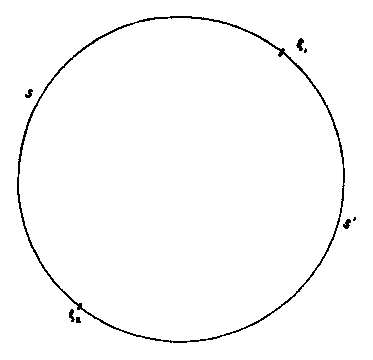
\includegraphics{chap04-vend-scan-01.eps}
\caption{Example of drifter trajectories.}\label{ch04:fig1}
\end{figure}


Figure~\ref{ch04:fig1} shows the trajectories of several drifters at the surface of the ocean. The positions were recorded daily. They are real life instances of passive tracer transport. The sequences:
\begin{equation*}
\mathbf{x}_{0},\,\mathbf{x}_{1},\,\mathbf{x}_{2},\,\cdots\cdots
\end{equation*}
formed by the successive positions of a drifter are the result of the sampling of continuous time trajectories $t\hookrightarrow \mathbf{x}(t)$, i.e.
\begin{equation*}
\mathbf{x}_{0}=\mathbf{x}(t_{0}),\,\mathbf{x}_{1}=\mathbf{x}(t_{1}),\,\mathbf{x}_{2}=\mathbf{x}(t_{2}),\cdots\cdots
\end{equation*}
for times $t_{0}=0,\,t_{1}=\Delta t,\,t_{2}=2\Delta t,\,\cdots$ for some sampling interval $\Delta t>0$. Saying that we are observing a passive tracer is merely saying that a given trajectory $t\hookrightarrow \mathbf{x}(t)$ is a solution of the equation of motion:
\begin{equation}
\label{ch04:eqn1.1} d\mathbf{x}(t)=\vec{\mathbf{v}}(t,\,\mathbf{x}(t))\,dt
\end{equation}
where $\vec{\mathbf{v}}(t,\,\mathbf{x})$\index{symbols}{$\vec{\mathbf{v}}(t,\mathbf{x})$} denotes the velocity of the the ocean at time $t$ at the point $\mathbf{x}$. Note that for the sake of simplicity we did not include a viscosity term in the equation of motion. This will be done later.

Some of the statistical properties of these Lagrangian trajectories (i.e. the solutions of the equation of motion) have been investigated in \cite{ch04:bib15} as bivariate time series and the consequences of the assumptions of time stationarity and space homogeneity of the models on the spectra of these series were tested.

We shall review part of the theoretical framework of the theory of random velocity fields with Gaussian statistics, we formulate precisely the mathematical assumptions of the physical models most widely accepted (incompressibility, Kolmogorov spectrum\index{index}{Kolmogorov!spectrum}, $\ldots$) and we address the simulations issues. The present study is intended for models where the external velocity field is \emph{time dependent}. This excludes the stationary models for which the random velocity field is independent of time. Nevertheless we shall have many asides to discuss some of the recent results of Majda \emph{et} $al$ reported in \cite{ch04:bib6}, \cite{ch04:bib7}, \cite{ch04:bib40}, \cite{ch04:bib33} and especially the papers \cite{ch04:bib26} and \cite{ch04:bib25} reporting on numerical computations. Even though most of these digressions are devoted to emphasize the differences between the time independent case and the models considered here, it is nevertheless clear that many of the ideas used in these works to deal with the space correlations and the spectral singularity are relevant to our considerations. In the time dependent case we review the massively parallel simulations reported in \cite{ch04:bib13}, the conjectures formulated and illustrated there and the theoretical results proved subsequently. In particular, we discuss the proof of the positivity of the upper Lyapunov exponent\index{index}{Lyapunov exponent!positivity|seealso{mixing}}\index{index}{Lyapunov exponent} of the Jacobian flow given in \cite{ch04:bib14} and the proof of the homogenization\index{index}{homogenization} of the Lagrangian trajectories given in \cite{ch04:bib17}. Finally, we discuss numerical estimates of the time evolution of the fractal dimension (Minkowski dimension to be specific) of the boundary of blobs of passive tracers transported by the flow and on the attempts to make the tracers feel the spectral singularity in the spectrum. Random velocity fields with non-Gaussian statistics have been considered in the literature. Most of the models which we know of are based on Poisson point processes\index{index}{Poisson!point processes}. For the definition and the first properties of some of these models, the interested reader may consult for example \cite{ch04:bib8} for the time independent case and \cite{ch04:bib21} and \cite{ch04:bib22} for the time dependent case. For these models, the time structure is still of the Ornstein-Uhlenbeck type and it is expected that most of the results proven for the Gaussian fields discussed in this chapter (strict positivity of the upper Lyapunov exponent of the Jacobian flow, exponential mixing, $\cdots$) will still hold. We end this chapter with a short discussion of the rationale behind these Poisson models.

All the numerical results reported in this chapter can be reproduced using a C - program available on the Web at the URL \cite{ch04:bib19}.

\section{Gaussian Velocity Fields with Kolmogorov Spectra}
\label{ch04:sec2}

We present the assumptions of a commonly used mathematical model of a random velocity field. Since the general considerations of this section do not depend upon the dimension of the space we shall consider velocity fields on the general Euclidean space $\mathbb{R}^{d}$. We restrict ourselves to the dimension $d=2$ from Section~\ref{ch04:sec4} below on.

We assume that $\{\vec{\mathbf{v}}(t,\,\mathbf{x});\,t\geq 0,\,\mathbf{x}\in \mathbb{R}^{d}\}$\index{symbols}{$\vec{\mathbf{v}}(t,\mathbf{x})$} is a mean zero Gaussian vector field with values in $\mathbb{R}^{d}$. The hypothesis on the mean is chosen in order to concentrate our efforts on the understanding of the random fluctuations around a mean deterministic motion.

We assume that the velocity field is homogeneous in space\index{index}{velocity field!homogeneous in space}. By this we mean that its distribution is invariant under the shifts of the space variable $\mathbf{x}$. In other words that, for each fixed $\mathbf{y}\in \mathbb{R}^{d}$:
\begin{equation*}
\{\vec{\mathbf{v}}(t,\,\mathbf{x}+\mathbf{y});\,t\geq 0,\,\mathbf{x}\in \mathbb{R}^{d}\}\qquad \mathrm{and}\qquad \{\vec{\mathbf{v}}(t,\,\mathbf{x});\,t\geq 0,\,x\in \mathbb{R}^{d}\}
\end{equation*}
have identical distributions. We also assume that the random velocity field is stationary\index{index}{velocity field!stationarity}, i.e. its distribution is invariant under the shifts of the time variable $t$. This means that, for each fixed $s\geq 0$:
\begin{equation*}
\{\vec{\mathbf{v}}(s+t,\,\mathbf{x});\,t\geq 0,\,\mathbf{x}\in \mathbb{R}^{d}\}\qquad \mathrm{and}\qquad \{\vec{\mathbf{v}}(t,\,\mathbf{x});\,t\geq 0,\,\mathbf{x}\in \mathbb{R}^{d}\}
\end{equation*}
have identical distributions. These three assumptions (Gaussian statistics, homogeneity and stationarity) are quite common in the random mathematical models of turbulent fluids. See for example \cite{ch04:bib47} or \cite{ch04:bib9}.

The distribution of the random field is completely characterized by its covariance tensor:
\begin{equation}
\label{ch04:eqn2.1} \mathbb{E}\{\vec{\mathbf{v}}(s,\,\mathbf{x})\otimes\vec{\mathbf{v}}(t,\, \mathbf{y})\}=\Gamma(t-s,\,\mathbf{y}-\mathbf{x}),\qquad\qquad s,\,t\geq 0,\quad \mathbf{x},\,\mathbf{y}\,\in \mathbb{R}^{d}.
\end{equation}
If $\Phi$ is a random variable (or more generally a random vector) over the probability space of the velocity field, we use the notation $\mathbb{E}\{\Phi\}$ for its expectation. Notice that $\Gamma(t,\,\mathbf{x})$ is a $d\times d$ matrix. Its entries are given by the cross-covariances of the components of $\vec{\mathbf{v}}$:
\begin{equation*}
\Gamma_{j,\ell}(t,\,\mathbf{x})=\mathbb{E}\{v_{j}(0,0)v_{\ell}(t,\,\mathbf{x})\},\qquad\qquad
j,\,\ell=1,\cdots,d.
\end{equation*}\index{symbols}{$\Gamma_{j,\ell}(t,\mathbf{x})$}

\subsection{Spectral Representation} The matrix $\Gamma(t,\,\mathbf{x})$ is the Fourier transform of a nonnegative definite matrix measure $\nu(d\omega,\, d\mathbf{k})$. As usual, we use $\omega$ to denote the frequency variable associated to the time variable $t$ and we use the variable $\mathbf{k}$ for the wave number variable associated to the space variable $\mathbf{x}$. We also assume that the entries of the covariance matrix are integrable. This guarantees the existence of densities $E_{j,\ell}(\omega,\,k)$\index{symbols}{$E_{j,\ell}(\omega,k)$} for the entries $\nu_{j,\ell}(d\omega,\,dk)$\index{symbols}{$\nu_{j,\ell}(d\omega,\,dk)$} of the matrix measure $\nu(d\omega,\, dk)$. In other words we have:
\begin{equation}
\label{ch04:eqn2.2} \Gamma(t,\,\mathbf{x})=\int_{\mathbb{R}}\int_{\mathbb{R}^{d}}e^{i(\omega t+\mathbf{k}\cdot \mathbf{x})}E(\omega,\,\mathbf{k})\ dw\ d\mathbf{k}
\end{equation}
for some matrix $E(\omega,\,\mathbf{k})=[E_{j,\ell}(w,\,\mathbf{k})]_{j,\ell=1,\cdots,d}$. Further assumptions on the spatial characteristics of the velocity field, such as \emph{incompressibility}\index{index}{velocity field!incompressibility} and \emph{isotropy}\index{index}{velocity field!isotropy} can be used to specify further the covariance $\Gamma(t,\,\mathbf{x})$. This is usually done in terms of the form of its Fourier transform $E(\omega,\,\mathbf{k})$. See for example \cite{ch04:bib9}, \cite{ch04:bib47} and/or \cite{ch04:bib6}. The assumptions of isotropy and incompressibility essentially determine the form of the spatial part of the covariance. But it might also be desirable to build the structure of the time dependence and the time correlation into the model. In particular one may want to make the velocity field Markovian\index{index}{velocity field!Markovian} in time. In this case we get:
\begin{equation}
\label{ch04:eqn2.3} E_{j,\ell}(\omega,\,\mathbf{k})=\frac{\beta(|\mathbf{k}|)}{w^{2}+\beta(|\mathbf{k}|)^{2}}\mathcal{E}(|\mathbf{k}|)\frac{1}{|\mathbf{k}|^{d-1}}\left(\delta_{j,\ell}-\frac{k_{j}k_{\ell}}{|\mathbf{k}|^{2}}\right),
\end{equation}
for some scalar functions $r\hookrightarrow\beta(r)$\index{symbols}{$\beta(r)$} and $r\hookrightarrow \mathcal{E}(r)$ of $r>0$. The type of function $\mathcal{E}(r)$\index{symbols}{$\mathcal{E}(r)$} used in fluid mechanics varies depending on the applications. Kolmogorov's theory of turbulence\index{index}{Kolmogorov!theory of turbulence} suggests a scale invariance which is brought into the model by the choice of a power function $\mathcal{E}(r)=r^{1-\epsilon}$ for some real parameter $\epsilon$. We shall restrict ourselves to the interesting case $\epsilon>0$. The classical Kolmogorov spectrum\index{index}{Kolmogorov!spectrum!classical} is associated to the value $\epsilon=5/3$ in $d=2$ dimensions. Since a power function cannot be integrable both at the origin and at infinity, this choice will lead to singularities which play a crucial role in the properties of the system and especially in the transport properties of such fluids.

Mathematical regularization of the singularities is usually achieved by the introduction of cut-off functions\index{index}{Kolmogorov!spectrum!cut-off}. In other words, the original function $\mathcal{E}(r)$ is replaced by a regularized form:
\begin{equation}
\label{ch04:eqn2.4} \mathcal{E}^{(reg)}(r)=\mathcal{E}(r)\chi_{0}(r)\chi_{\infty}(r)
\end{equation}\index{symbols}{$\mathcal{E}^{(reg)}(r)$}
where the infrared cut-off function $\chi_{0}(r)$ vanishes near the origin and the ultraviolet cut-off function $\chi_{\infty} (r)$ vanishes near $\infty$. When the function $\mathcal{E}(r)$ is chosen to be zero near the origin (i.e. for $r\leq r_{0}$ for some $r_{0}>0$) and near infinity (i.e. for $r\geq r_{1}$ for some $r_{1}<\infty$) we shall say that the velocity field is regular. The value of the parameter\index{index}{Kolmogorov!spectrum!parameters} $\epsilon$ controls the spatial correlation in the velocity field. In the classical Kolmogorov's theory, the numbers $r_{0}$ and $r_{1}$ are related to the so-called integral and dissipation scales\index{index}{Kolmogorov!theory of turbulence!integral and dissipation scales}\index{index}{integral!scale}\index{index}{dissipation scale} respectively.

The function $\beta(r)$ is usually chosen of the form:
\begin{equation*}
\beta(r)=r^{z}
\end{equation*}
for some $z>0$. In this way, the parameter $z$\index{symbols}{$z$} controls the time correlation in the velocity field. As a consequence, a Kolmogorov's spectrum can be characterized by the two parameters $z$ and $\epsilon$\index{symbols}{$\epsilon$}. Finally we recall the spectral representation formula:
\begin{equation}
\label{ch04:eqn2.5} \vec{\mathbf{v}}(t,\,x)=\int_{\mathbb{R}}\int_{\mathbb{R}^{d}}e^{i(\omega
t+\mathbf{k}\cdot \mathbf{x})}E(\omega,\,\mathbf{k})^{1/2}W(d\omega,\,d\mathbf{k}).
\end{equation}
which writes the random velocity field in terms of a complex vector white noise measure (in the $L^{2}$-sense) $W(d\omega,\,d\mathbf{k})$.

\section{Abstract Ornstein Uhlenbeck Velocity Fields}
\label{ch04:sec3}

In order to motivate the introduction of Ornstein Uhlenbeck (O-U for short) processes we revisit formula (\ref{ch04:eqn2.5}) giving the spectral representation of the velocity field. Performing the integration with respect to ($\omega$ in (\ref{ch04:eqn2.2}) gives:
\begin{equation*}
\Gamma(t,\mathbf{x})=\int_{\mathbb{R}^{d}}e^{i\mathbf{k}\cdot\mathbf{x}}E(t,\, \mathbf{k})\,d\mathbf{k}
\end{equation*}
with:
\begin{equation}
\label{ch04:eqn3.1} E_{j,\ell}(t,\,\mathbf{k})=e^{-|k|^{z}|t|}\mathcal{E}(|\mathbf{k}|)\frac{1}{|\mathbf{k}|^{d-1}}\left(\delta_{j,\ell}-\frac{k_{j}k_{\ell}}{|\mathbf{k}|^{2}}\right).
\end{equation}
In other words, the covariance is in the Fourier domain the superposition of the covariances of O-U processes and it is natural to conjecture that the spectral representation (\ref{ch04:eqn2.5}) can be rewritten in the form:
\begin{equation}
\label{ch04:eqn3.2} \vec{\mathbf{v}}(t,\,\mathbf{x})=\int_{\mathbb{R}^{d}}e^{i\mathbf{k}\cdot \mathbf{x}}\tilde{E}(\mathbf{k})^{1/2}\xi_{t}(d\mathbf{k}).
\end{equation}
where the $\xi_{t}(d\mathbf{k})$ are, for each fixed $t$, orthogonal (independent) increment $L^{2}$-measures in the Fourier domain and for each fixed infinitesimal $d\mathbf{k}$, OU processes in the time variable. This fact can be proven rigorously using the theory of $L^{2}$ martingale measures as developed in \cite{ch04:bib46}. But most importantly, the very form of the representation (\ref{ch04:eqn3.2}) shows that, if we look at $\vec{\mathbf{v}}(t,\,\mathbf{x})$ as a function of $\mathbf{x}$, say $\vec{\mathbf{v}}(t)=\vec{\mathbf{v}}(t,\, \cdot)$ for each fixed time $t$, then the process $\{\vec{\mathbf{v}}(t);\,t\geq 0\}$ should be regarded as a form of Ornstein Uhlenbeck process with values in a space of functions of $\mathbf{x}$, possibly of infinite dimensions since it appears as the result of a linear superposition (i.e. an integral) of many such processes.

\subsection{The Abstract Set-Up}\label{ch04:sec3.1} Let $A$ and $B$ be two nonnegative self-adjoint operators on a separable Hilbert space $H$. For the sake of simplicity we shall assume that the operators $A$ and $B$ commute and for each $t\geq 0$ we consider the self-adjoint operator:
\begin{equation*}
\Gamma(t)=B(2A)^{-1}e^{-tA}.
\end{equation*}
Even though $e^{-tA}$ is a contraction, the operator $\Gamma(t)$ may be unbounded and delicate domain problems may occur. Nevertheless, we shall keep the present discussion to a formal level and we shall ignore these domain questions until we get to the specific examples discussed in the next subsection. The nonnegative operator $\Gamma(0)=B(2A)^{-1}$ can be viewed as the covariance operator of a mean zero (possibly only additive) Gaussian measure on $H$. Enlarging $H$ if necessary, this measure can be extended into a $\sigma$-additive bona-fide measure, say $\nu$. Let us denote by $\tilde{H}$ such an enlargement of $H$. The operators $\Gamma(t)$ can then be used to construct a $\tilde{H}$ - valued mean zero Gaussian process, say $\{\mathbf{v}(t);\,t\geq 0\}$, such that the covariance of $\mathbf{v}(s)$ and $\mathbf{v}(t)$ is given by the operator $\Gamma(|t-s|)$. This statement will be made more precise in the following subsection when we discuss specific examples. Specific assumptions and gory details of this abstract construction are given in \cite{ch04:bib4} where it is also shown that it is possible to view the process as the solution of a stochastic differential equation (in an infinite dimensional space) of the standard form:
\begin{equation}
\label{ch04:eqn3.3} d\mathbf{v}(t)=-A\mathbf{v}(t)dt+dW_{B}(t)
\end{equation}
where $\{W_{B}(t);\,t\geq 0\}$ is a process of Brownian motion with covariance $B$ in the sense that the operator $B$ is the covariance operator of the (infinite dimensional) random variable $W_{B}(1)$. This process of Brownian motion does not need to be taking its values in the space $\tilde{H}$ as long as its values are mapped back into this space by the operator semigroup $e^{-tA}$ as formula (\ref{ch04:eqn3.4}) shows. In any case, this infinite dimensional O-U process also has the following integral representation:
\begin{equation}
\label{ch04:eqn3.4} \mathbf{v}(t)=\mathbf{v}(0)+\int_{0}^{t}e^{-(t-s)A}dW_{B}(s)
\end{equation}
where the integral is given the usual sense of the classical theory of the Wiener integral except that we are dealing here with an operator valued integrand and a function valued integrator.

\subsection{O-U Velocity Fields}\label{ch04:sec3.2} We now consider specific instances of the general model described above and we show how this framework includes the incompressible Gaussian velocity fields with Kolmogorov spectra.

The first example we have in mind is the following. $H=L^{2}(\mathbb{R}^{d},\, dx)$ is the classical Hilbert space of (equivalent classes) of square integrable complex functions on the Euclidean space $\mathbb{R}^{d},\,A=(-\Delta)^{z/2}$ is a power of the negative Laplacian (at this stage $z$ can be any nonnegative real number) and $B=\mathcal{E}((-\Delta)^{1/2})$ is a specific nonnegative function of the same self-adjoint operator $-\Delta$. The fact that both $A$ and $B$ appears as functions of the same self-adjoint operator ensures that $A$ and $B$ commute. Specific properties of the nonnegative function $r\hookrightarrow \mathcal{E}(r)$ on the half-axis $(0,\,\infty)$ will be discussed later but we use the same notation $\mathcal{E}(r)$ as earlier for obvious reasons: this function is very much related to the functions $\mathcal{E}$ and $\mathcal{E}^{(reg)}$ introduced earlier and to the functions $\mathcal{E}_{\phi}$ and $\mathcal{E}_{\phi}^{(reg)}$ discussed below.

To identify further the infinite dimensional O-U process $\mathbf{v}(t)$ constructed above to the velocity fields with Kolmogorov spectra, we assume that the spectral function $\mathcal{E}(r)$ is bounded, has bounded support and that this support is bounded away from 0. This is the case for the function $\mathcal{E}_{\phi}^{(reg)}(r)$ introduced in the next section to analyze the stream function\index{index}{stream function} in dimension $d=2$. In this case, $B$ is a bounded operator on $H$ with a spectrum bounded away from $0$ (and in particular with a bounded inverse.) More importantly, the compactness of the support makes it possible to choose $\tilde{H}$ as a space of analytic functions. If we then denote by $\mathbf{v}(t,\,\mathbf{x})$ the value of the function $\mathbf{v}(t)$ resulting from the construction outlined in the previous subsection, at the point $\mathbf{x}\in \mathbb{R}^{d}$, then one has:
\begin{equation*}
\mathbb{E}\{\mathbf{v}(s,\,\mathbf{x})\mathbf{v}(t,\,\mathbf{y})\}=\Gamma(t-s,\, \mathbf{y}-\mathbf{x})\,=[\mathcal{E}((-\Delta)^{1/2})e^{-|t-s|\Delta^{z/2}}](x-y)
\end{equation*}
if we use the notation $\Gamma(t,\,\cdot)$ for the integral kernel of the operator $\Gamma(t)$. If we now go to the Fourier domain to express the kernel of this function of the negative Laplacian we get:
\begin{equation*}
\mathbb{E}\{\mathbf{v}(s,\,\mathbf{x})\mathbf{v}(t,\,\mathbf{y})\}=\int_{\mathbb{R}^{d}}e^{i\mathbf{k}\cdot(\mathbf{y}-\mathbf{x})}\mathcal{E}(|\mathbf{k}|)e^{-|t-s||\mathbf{k}|^{z}}\,d\mathbf{k}
\end{equation*}
which is of the desired form (with $\beta(r)=r^{z}$) if we use the Fourier transform in time to express the exponential $e^{-|t-s||\mathbf{k}|^{z}}$. The field $\mathbf{v}(t,\,\mathbf{x})$ so defined (as well as its covariance function $\Gamma(t,\,\mathbf{x}))$ is scalar so strictly speaking, this construction applies only to the two dimensional case of the stream function $\phi(t,\, \mathbf{x})$ introduced and analyzed in the next section. In the general case, one needs to consider a Hilbert space $H$ of vector valued functions (by tensor products for example) and have the operators $A$ and $B$ act appropriately. These operators can be chosen as functions of the negative Laplacian as well and the construction of the infinite dimensional O-U process $\mathbf{v}(t)$ can be done in this case also and one can then recover a vector random field $\mathbf{v}(t,\,\mathbf{x})$ which has a spectrum of the same structure as the velocity field $\vec{\mathbf{v}}(t,\,\mathbf{x})$ we started from in the introduction.

\section{Simulation of the Velocity Field}
\label{ch04:sec4}

From now on we restrict ourselves to the 2 - dimensional case. Because of the incompressibility assumption, this restriction implies that the velocity field can be derived from a \emph{stream function} $\phi(t,\,\mathbf{x})$\index{symbols}{$\phi(t,\mathbf{x})$} via the formula:
\begin{equation*}
\vec{\mathbf{v}}(t,\,\mathbf{x})=\left[\begin{array}{l}
\frac{\partial\phi(t,\mathbf{x})}{\partial x_{2}}\\
\frac{-\partial\phi(t,\mathbf{x})}{\partial x_{1}}
\end{array}\right].
\end{equation*}
The scalar random field $\{\phi(t,\,\mathbf{x});\,t\geq 0,\,\mathbf{x}\in \mathbb{R}^{2}\}$ can be chosen to be stationary in time and homogeneous in space. In fact a formula similar to (\ref{ch04:eqn3.2}) can be derived and the stream random field can be used in the form (at least in distribution):
\begin{equation}
\label{ch04:eqn4.1} \phi(t,\,\mathbf{x})=\int_{\mathbb{R}^{2}}e^{i\mathbf{k}\cdot \mathbf{x}}\sqrt{\tilde{E}_{\phi}(\mathbf{k})}\xi_{t}(d\mathbf{k}).
\end{equation}
where the function $\tilde{E}_{\phi}(\mathbf{k})$ is now a scalar function instead of being a matrix valued function. This ``special spectral representation'' can be undone to recover the standard spectral representation of the stream function. We get:
\begin{equation}
\label{ch04:eqn4.2} \phi(t,\,\mathbf{x})=\int_{\mathbb{R}^{2}}e^{i\mathbf{k}\cdot \mathbf{x}}\sqrt{E_{\phi}(\omega,\,\mathbf{k})}W^{\prime}(dw,\,d\mathbf{k})
\end{equation}
where $W^{\prime}(d\omega,\,d\mathbf{k})$ is a scalar valued orthogonal $L^{2}$ white noise measure and where the (scalar) spectral density $E_{\phi}(\omega,\, \mathbf{k})$\index{symbols}{$E_{\phi}(\omega,\, \mathbf{k})$} is of the form:
\begin{equation}
\label{ch04:eqn4.3} E_{\phi}(\omega,\,\mathbf{k})=\frac{\beta(|\mathbf{k}|)}{\omega^{2}+\beta(|\mathbf{k}|)^{2}}\mathcal{E}_{\phi}(|\mathbf{k}|)
\end{equation}
in full analogy with (\ref{ch04:eqn2.3}). Simple arithmetic gives:
\begin{equation}
\label{ch04:eqn4.4} \mathcal{E}_{\phi}(r)=r^{-3}\mathcal{E}(r)
\end{equation}\index{symbols}{$\mathcal{E}_{\phi}(r)$}
if $\mathcal{E}(r)$ stands for the spectral function introduced in (\ref{ch04:eqn3.1}).

\subsection{Abstract Formalism}\label{ch04:sec4.1} We first present the general form of the simulation algorithm. Because we plan to simulate the Ornstein Ulhenbeck process at successive times, we take advantage of the Markov property and we derive a formula to update the process. Coming back to the integral representation (\ref{ch04:eqn3.4}) we see that, whenever $t$ and $h$ are nonnegative we have:
\begin{align*}
\phi(t+h) &= e^{-hA}\left(e^{-tA}\phi(0)+\int_{0}^{t}e^{-(t-s)A}W_{B}(ds)\right)+\int^{t+h}_{t}e^{-(t+h-s)A}W_{B}(ds)\\
&=e^{-hA}\phi(t)+\int^{t+h}_{t}e^{-(t+h-s)A}W_{B}(ds).
\end{align*}

Not only this formula proves the Markov property (in time) of the process but it also provides a simple formula for the transition probability of the process. Indeed, the conditional distribution of $\phi(t+h)$ given the past $\mathcal{F}_{t}$ of the process up to time $t$ is the Gaussian distribution with mean $e^{-hA}\phi(t)$ and covariance equal to the covariance of the stochastic (Wiener) integral:
\begin{equation}
\label{ch04:eqn4.5} \int^{t+h}_{t}e^{-(t+h-s)A}W_{B}(ds).
\end{equation}
Given the definition of the process $W_{B}$, the latter is given by:
\begin{equation}
\label{ch04:eqn4.6} \Gamma_{h}(f,\,g)=\int_{0}^{h}<Be^{-sA}f,\,g\,>ds
\end{equation}
where the notation $<\cdot,\,\cdot>$ is used for the $H$-inner product. Hence the update procedure can be summarized in the following way:
\begin{itemize}
\item generate $\phi(0)$ with distribution $\nu$ (i.e. as a mean zero Gaussian random variable with covariance:
\begin{equation}
\label{ch04:eqn4.7} \Gamma_{0}(f,\,g)=<B(2A)^{-1}f,\,g>.
\end{equation}
\item given a realization of $\phi(t)$ generate a realization of $\phi(t+h)$ as a Gaussian random variable with mean
\begin{equation}
\label{ch04:eqn4.8} \mu_{t+h}=e^{-hA}\phi(t)
\end{equation}
and covariance $\Gamma_{h}$ given in (\ref{ch04:eqn4.6}).
\end{itemize}

\begin{remark}\label{ch04:rem4.1}The second bullet deals with the update of the stream function\index{index}{discretization!stream function} (and hence of the velocity field) as time evolves. Obviously, this step is not present in the analysis of time independent velocity fields. But as we shall see later, this is not the only reason simulations are much easier to set up in the time independent case.
\end{remark}

\subsection{Time Discretization and Expansion in a Basis}\index{index}{discretization!time}\label{ch04:sec4.2} The idea is to discretize the time into a sequence $(t_{n})_{n=0,1,\cdots}$ and to use the Markov property to construct the next value $\vec{\mathbf{v}}(t_{n+1})$ from the current value $\vec{\mathbf{v}}(t_{n})$ ignoring the way the field ``got there'' i.e. ignoring the values of $\vec{\mathbf{v}}(t_{0}),\,\vec{\mathbf{v}}(t_{1}),\,\cdots,\vec{\mathbf{v}}(t_{n-1})$. Moreover, since each $\vec{\mathbf{v}}(t)$ is itself an infinite dimensional object, we shall need to use other finite dimensional approximations to construct the configurations $\vec{\mathbf{v}}(t)$.

The discretization of time is straightforward. We choose a time interval $\Delta t$ and we sample the continuous time by restricting its values to:
\begin{equation*}
t_{0}=0,\,t_{1}=\Delta t,\,t_{2}=2\Delta t,\,\cdots,\,t_{n}=n\Delta t,\,\cdots\cdots
\end{equation*}
Because of the Markov property and because of our choice for the discretization of the time, at each instant $t_{j}$, we will use the knowledge of the characteristics of the field $\vec{\mathbf{v}}(t_{j-1})$ at the preceding time to generate the samples of the velocity field $\vec{\mathbf{v}}(t_{j},\,\mathbf{x})$ at the locations $\mathbf{x}$ where we need them. Notice that the choice of the time interval $\Delta t$ has to depend upon the spectral characteristics, and especially of the radial lower bound $r_{0}$ on the support of the spectral density. This remark will be especially useful when we simulate velocity fields for different values of the spectral parameters $\epsilon$ and $z$. See the discussion of the renormalization problems in the last section below for details.

We now consider a more precise form of the simulation algorithm, still without paying much attention to the actual convergence of the formal expansions we use. Since we restrict ourselves to dimension $d=2$ we find it more convenient to work with the stream function.

Let $(\varphi_{n})_{n\geq 1}$ be a complete orthonormal system in $H$ and let us expand the O-U process $\{\phi(t);t \geq 0\}$ as if it were an element of the Hilbert space. At each time $t$ we want to take advantage of the expansion:
\begin{equation}
\label{ch04:eqn4.9} \phi(t)=\sum\limits_{n=0}^{\infty}<\phi(t),\,\varphi_{n}>\varphi_{n}.
\end{equation}
Our goal is to replace the sum of the infinite series (\ref{ch04:eqn4.9}) is replaced by a finite sum. In particular we simulate the initial value $\phi(0)$ as:
\begin{equation}
\label{ch04:eqn4.10} \tilde{\phi}(0)=\sum\limits_{n=0}^{N_{0}}<\phi(0),\,\varphi_{n}>\varphi_{n}=\sum\limits_{n=0}^{N_{0}}\xi_{n}^{(0)}\varphi_{n}
\end{equation}
provided we set $\xi_{n}^{(0)}=<\phi(0),\,\varphi_{n}>$. These random variables form a Gaussian sequence of mean zero random variables. Their covariance matrix is given by the matrix elements:
\begin{equation}
\label{ch04:eqn4.11} \gamma^{(0)}(m,\,n)=\mathbb{E}\{\xi_{m}^{(0)}\xi_{n}^{(0)}\}=<B(\varphi_{m},\,\varphi_{n}>.
\end{equation}
In particular, the sequence $\xi^{(0)}=\{\xi_{n}^{(0)};\,n =0,\cdots,N_{0}\}$ is independent if the orthonormal basis $\{\varphi_{n}\}_{n}$ is formed of eigenvectors of the self-adjoint operator $B$. In this case the variance of $\xi_{n}^{(0)}$ is merely the $n$-th eigenvalue (as usual counting multiplicity) i.e. the eigenvalue corresponding to the eigenfunction $\varphi_{n}$, and the generation of the $\xi_{n}^{(0)}$'s is very simple if these eigenvalues are known. Otherwise, the \emph{matrix elements} $<B\varphi_{m},\,\varphi_{n}>$ have to be computed, the square root of the matrix $\gamma^{(0)}=[\gamma^{(0)}(m, n)]_{m,n=1,\cdots N_{0}})$ has to be computed and the vector $\xi^{(0)}$ of dimension $(N_{0}+1)$ can be generated as:
\begin{equation*}
\xi^{(0)}=\sqrt{\gamma^{(0)}}\eta^{(0)}
\end{equation*}
where $\eta^{(0)}$ is a $(N_{0}+1)$-dimensional vector of i.i.d. $N(0,1)$ random variables.

Let us now consider the problem of the update of the process. Let us assume that the generation of the process at time $t=j\Delta t$ has been done according to the formula:
\begin{equation*}
\tilde{\phi}(j)=\sum\limits_{n=0}^{N_{j}}\xi_{n}^{(j)}\varphi_{n}
\end{equation*}
for some sequence $\{\xi_{n}^{(j)};\,n=0, \cdots, N_{j}\}$ of real numbers. Obviously, this sequence forms a realization of a Gaussian sequence with a specific mean $\mu^{(j)}$ and covariance matrix $\gamma^{(j)}$. According to the discussion of the previous section, the next value $\tilde{\phi}(j+1)$ of the stream function at time $t_{j+1}=(j+1)\Delta t$ is constructed as the sum of a (conditional) mean $\mu^{(j+1)}$ and a fluctuating part. First we compute its mean. We choose the approximation of $e^{-(\Delta t)A}\phi(n\Delta t)$ obtained by replacing $\phi(n\Delta t)$ by the element of $H$ whose components in the $\{\varphi_{n}\}_{n}$ basis are given by the components of the vector $\mu^{(j)}$. In other words we use the mean:
\begin{align}
\mu^{(j+1)}&=e^{-(\Delta t)A}\sum\limits_{n=0}^{N_{j}}\xi_{n}^{(j)}\varphi_{n}\\
\label{ch04:eqn4.12} &=\sum\limits_{m=0}^{N_{j+1}}\left(\sum\limits_{n=0}^{N_{j}}<e^{-(\Delta t)A}\varphi_{n},\,\varphi_{m}>\xi_{n}^{(j)}\right)\varphi_{m}
\end{align}

In order to compute the fluctuating part we compute the matrix elements of the covariance operator $\Gamma_{\Delta t}$ on the basis elements $\varphi_{n}$ (recall formula (\ref{ch04:eqn4.6}).
\begin{equation*}
\gamma^{(j+1)}(m,\,n)=\int_{0}^{\Delta t}<Be^{-sA}\varphi_{m},\,\varphi_{n}>ds
\end{equation*}
and we proceed as when we generated $\xi^{(0)}$: we first compute the square root of the matrix $\gamma^{(j+1)}$, then we generate i.i.d. standard Gaussian random variables and we multiply the vector so-obtained by the square root of $\gamma^{(j+1)}$.

A naive approach to the discretization of the space variable could be to use expansions into ``\emph{bases of delta functions}.'' In the same way we replaced the continuous time $t$ by a grid of discrete values, it is possible to replace the space variable $\mathbf{x}\in \mathbb{R}^{2}$ by a discrete variable taking finitely many values in a lattice $h\mathbb{Z}^{2}$ for some mesh $h>0$. This strategy has several drawbacks, especially from the point of view of Monte-Carlo simulation. Indeed, for each fixed time $t$, there is a strong dependence between the values of $\vec{\mathbf{v}}(t,\,\mathbf{x})$ and $\vec{\mathbf{v}}(t,\,\mathbf{y})$ even when the points $\mathbf{x}$ and $y$ are far apart, making the generation of the configuration $\vec{\mathbf{v}}(t_{j})$ from $\vec{\mathbf{v}}(t_{j-1})$ extremely costly in memory storage and in computing time: this approach is not reasonable for our application.

Most importantly, the transport simulations which we discuss below require updates of passive tracers at each time step. These updates force us to compute the velocity field at the positions of the tracers and the latter do not have the good taste of staying on the points of the lattice $h\mathbb{Z}^{2}$. An artificial extrapolation would be needed in order to get the values of the velocity field necessary for the updates and we shall refrain from doing that.

\subsection{Wavelet Expansions}\label{ch04:sec4.3} As we have already emphasized, the initialization of the simulation process for the velocity field is the computation of the partial expansion (\ref{ch04:eqn4.9}):
\begin{equation*}
\tilde{\phi}(0)=\sum\limits_{n=0}^{N_{0}}\xi_{n}^{(0)}\varphi_{n}
\end{equation*}
where the $\varphi_{n}$'s form a basis of the space and the $\xi_{n}^{(0)}$'s form a mean zero Gaussian sequence with a covariance matrix given by the matrix elements of the operator $B$ in the basis $\{\varphi_{n}\}_{n}$. At this stage, any orthonormal system would do essentially as well. In the time - independent case considered in \cite{ch04:bib26} and \cite{ch04:bib25} wavelet like bases were used. This last paper contains blunt propaganda for the choice of Meyer's wavelet. Given the fact that the authors consider a shear flow\index{index}{shear!flow} model (and hence a scalar field parameterized by a one-dimensional space variable) this choice should be obvious if one keeps in mind the fact that the mean square error $\mathbb{E}\{|v(0)-\tilde{v}(0)|^{2}\}$ is essentially the integral over the wave number space of the square difference between the spectral density and the Fourier transform of the partial expansion in the basis. Because of the special form of Meyer's wavelet and the fact that one can explicitly control the effects of scaling and translation in the Fourier domain, it is reasonable to consider paying the price of the construction of the correlation structure in the coefficients in the decomposition. But most importantly, the attractiveness of the wavelet decomposition is due to the presence of the spectral singularity of the model. Indeed, since all the elements of a wavelet basis \emph{vanish} at the origin in the Fourier domain, replacing the infinite sum of (\ref{ch04:eqn4.9}) by the finite sum (\ref{ch04:eqn4.10}) kills two birds with one stone. Not only does the wavelet decomposition provide a \emph{spatial discretization} suitable for numerical implementation but it also provides an algorithmic way to implement the spectral cut - off: this seems to be the ideal way to feel the effect of the spectral singularity. Majda and his students have used this idea to compute the structure function\index{index}{structure function}:
\begin{equation}
\label{ch04:eqn4.13} \mathbb{E}\{[v(x)-v(y)]^{2}\}
\end{equation}
in the case of a scalar time independent Gaussian process $\{v(x);\,x\in \mathbb{R}\}$ of the fractional Brownian type\index{index}{fractional Brownian process} which they use for the nontrivial component of a shear flow velocity field. A simple Gaussian computation shows that the structure function can be computed without the cut-off and that it is a specific power of $|x-y|$, namely:
\begin{equation}
\label{ch04:eqn4.14} \mathbb{E}\{[v(x)-v(y)]^{2}\}=c|x-y|^{2h-1},
\end{equation}
if the spectral density of the scalar mean zero Gaussian (generalized) process is $|k|^{-3h}$. These authors use an expansion in the Meyer's wavelet basis to recover numerically this asymptotic with Monte Carlo computations of the expectation appearing in the definition (\ref{ch04:eqn4.13}) of the structure function. Another very appealing feature of the structure function computation is that \emph{one knows ahead of time where the velocity field will have to be computed} and this can be taken advantage of in the setting up of the computations. Indeed, knowing $x$ and $y$ (by homogeneity, the computation is in fact done for $0$ and $y-x$) one can determine, for each resolution the set of wavelet coefficients which will not be zero and limit the generation of the Gaussian random variable to these coefficients. The effect of this innocent looking remark is to increase the efficiency and the precision of the computations.

It is conceivable to consider the generalization of the numerical computation of the structure function to the more general case of isotropic flows. The Meyer's wavelet basis will have to be replaced by a basis of functions on the two-dimensional plane, and using tensor products is a natural way to construct such functions. Even though the isotropy will have to be lost in such an expansion, we believe that this generalization is possible. But our main concern is the implementation of these ideas in the time - dependent case.

The level of complexity of the generation of samples from the velocity field in the time - independent case is the same as the level of complexity of the generation of samples of $\phi(0)$ in the time dependent case. But in the time - dependent case, there is a enormous computing overhead due to the update of the field as time evolves and especially for building the time and space correlations. The general discussion of the previous section gives the general framework and it seems reasonable to try to implement it as long as the matrix elements of the operators $B$ and $e^{-(\Delta t)A}$ can be computed in the \emph{wavelet} basis. Formula (\ref{ch04:eqn4.12}) giving the update of the mean of the stream function is amenable to wavelet expansions because since $(\Delta t)$ is small, one can use the approximation $e^{-(\Delta t)A}\approx I-(\Delta t)A$ to argue that the matrix representing the operator $e^{-(\Delta t)A}$ in the wavelet basis will be sparse (recall that both $A$ and $B$ are functions of the negative Laplacian $-\Delta$.)

We refrained from doing so because we are not only interested in the asymptotics of the Eulerian structure function, but we are mostly interested in the transport properties of the flow. As we will see shortly, it is impossible to know exactly in advance where the velocity field will have to be computed (i.e. where the tracer particles will be.) Given a finite time horizon, it is possible to estimate \emph{with high probability} where \emph{most} of the particles will be, but it is impossible to do that with certainty. Only in the case of a shear flow\index{index}{shear!flow} can this be done when the diffusivity $\kappa$ is zero. This is the particular situation considered in \cite{ch04:bib25} to compute the mean square displacement of two particles. But unfortunately, short of being able to control this set it is not possible to limit the set of wavelet coefficients which will enter significantly in the computation and the latter become infeasible.

In contrast, the Fourier expansions described below have enough built in independence for the computational burden to be minimal for regular models, and in particular when one does not attempt to feel the effect of the singularity. But before we give up on wavelet expansions, we would like to identify one more of the subtle pitfalls of this arena. Given a finite set of tracers to transport and a finite time horizon, it seems reasonable to work out the update of the statistical correlations of the velocity field in the following way: at each time step one uses the knowledge of the positions of the tracers to determine which of the coefficients of the wavelet expansion will be significant and one restricts the random generation of the coefficients to these basis components. It seems reasonable to expect that a very meticulous book-keeping should make it possible to track these basis coefficient labels. But unfortunately, running the random generation from them would lead to the Monte Carlo simulation of some sort of Lagrangian distribution of the velocity field in lieu of the desired Eulerian statistics!

\subsection{Fourier Expansions}\label{ch04:sec4.4} This section is devoted to the description of the simulation of a random velocity field of the Kolmogorov type when cut-off functions have been used to remove the infrared and ultraviolet singularities of the spectrum. In this case the infinite dimensional Ornstein Ulhenbeck process is regular in the sense that the operator $B$ is bounded, its spectrum is bounded away from zero and as a consequence, the operator $A$ can be treated as bounded. In the same way we considered expansions in ''\emph{bases of delta functions}'' in the space domain, one can contemplate expansions in ''\emph{bases of delta functions}'' in the Fourier domain\index{index}{discretization!Fourier domain}. This approach is not restrictive for regular fields and it is very much in the spirit of the spectral theory of stationary and/or homogeneous random fields, the simplest approach is to approximate the spectral measure $\nu(d\omega,\,dk)$ by simpler measures more amenable to random simulations on a computer. In particular, it is natural to approximate $\nu$ by a finite sum of point masses $\delta_{(\omega_{i},k_{i})}$ in the frequency-wave number domain. This approach is especially useful because it makes it possible to simulate directly the white noise without any concern with the possible dependence of the random variates to generate. Nevertheless, we refrain from using this approach directly, especially in the time variable. Indeed, in order to save memory (and computing time) we want to use an adaptive approach generating new values of the velocity field as we need them. More precisely, we want an approximation scheme which uses the fact that $\vec{\mathbf{v}}(t)$ is a time homogeneous Markov process. For this reason we shall separate the problems of the discretization of the time and the space variables.

Instead we shall use a strategy based on the ''nonstandard spectral representation formula'' (\ref{ch04:eqn4.1}). We choose a finite partition of the support of the function $\mathcal{E}_{\phi}(|\mathbf{k}|)$, say $\mathcal{D}=\{D_{\mathbf{k}};\,\mathbf{k}\in \mathcal{K}\}$ where the parameter $\mathcal{K}$ is viewed as a set of wave vectors in $\mathbb{R}^{2}$ (typically we shall make sure that $\mathbf{k}\in D_{\mathbf{k}}$.) We then construct an approximation in the form:
\begin{equation}
\label{ch04:eqn4.15} \phi_{\mathcal{K}}(t,\,\mathbf{x})=\sum\limits_{\mathbf{k}\in \mathcal{K}}e^{i\mathbf{k}\cdot \mathbf{x}}e(\mathbf{k})\xi_{t}(D_{\mathbf{k}})
\end{equation}\index{symbols}{$\phi_{\mathcal{K}}(t,\mathbf{x})$}\index{symbols}{$\xi_{t}$}
where the $e(\mathbf{k})$'s are coefficients obtained by taking the square root of the integral of the function $\mathcal{E}_{\phi}(|\mathbf{k}|)$ over the patch $D_{\mathbf{k}}$. Notice that the $\{\xi_{t}(D_{\mathbf{k}});\,t\geq 0\}$ are independent Ornstein Uhlenbeck processes. The choice of the partition $\mathcal{D}$, of the set $\mathcal{K}$ of wave vectors and of the corresponding approximate spectral coefficients $e(\mathbf{k})$ have a strong influence on the qualities of the approximation of the stream function and consequently on the velocity field itself and the corresponding transport properties of the flow. Nevertheless, except for the particular case of a set $\mathcal{K}$ contained in a line, most of the qualitative properties which we want to illustrate by numerical simulations are stable when one varies these choices.

Formula (\ref{ch04:eqn4.15}) is written with the continuous variable $t$, but as we explained earlier the time variable will be sampled on a regular grid. The effect of the sampling will just be to turn the continuous time Ornstein Uhlenbeck processes into discrete time autoregressive processes of order 1. See below for details.

Simple arithmetic on formula (\ref{ch04:eqn4.15}) leads to the real representation:
\begin{equation}
\label{ch04:eqn4.16} \phi(t,\,\mathbf{x})=\sum\limits_{\mathbf{k}\in \mathcal{K}}[a_{\mathbf{k}}(t)\cos(\mathbf{k}\cdot \mathbf{x})+b_{\mathbf{k}}(t)\sin(\mathbf{k}\cdot \mathbf{x})]
\end{equation}
where the $\{a_{\mathbf{k}}(t);\,t\geq 0\}$ and the $\{b_{\mathbf{k}}(t);\,t\geq 0\}$ are independent scalar Ornstein Uhlenbeck processes. As explained below, the latter become auto regressive processes after discretization of the time using the simplest Euler scheme\index{index}{Euler scheme}\index{index}{discretization!Euler scheme}. The components $v_{1}(t,\,\mathbf{x})$ and $v_{2}(t,\,\mathbf{x})$ of the velocity vector $\vec{\mathbf{v}}(t,\,\mathbf{x})$ can then be computed according to the formulas:
\begin{equation}
\label{ch04:eqn4.17} v_{1}(t,\,\mathbf{x})=\sum\limits_{\mathbf{k}\in \mathcal{K}}k_{2}[a_{\mathbf{k}}(t)\sin(\mathbf{k}\cdot \mathbf{x})-b_{\mathbf{k}}(t)\cos(\mathbf{k}\cdot \mathbf{x})]
\end{equation}
and:
\begin{equation}
\label{ch04:eqn4.18} v_{2}(t,\,\mathbf{x})=\sum\limits_{\mathbf{k}\in \mathcal{K}}k_{1}[-a_{\mathbf{k}}(t)\sin(\mathbf{k}\cdot \mathbf{x})+b_{\mathbf{k}}(t)\cos(\mathbf{k}\cdot \mathbf{x})].
\end{equation}
As formula (\ref{ch04:eqn5.2}) shows, we shall need to compute the velocity field at the instants $t_{j}$ at the positions $\mathbf{x}_{j-1}$ of the tracer particle. But notice that, once the program has knowledge of the auto-regressive\index{index}{auto-regressive} processes $a_{\mathbf{k}}$ and $b_{\mathbf{k}}$ labeled by the set $\mathcal{K}$ of wave vectors, the velocity field can be computed at \textbf{any} point $\mathbf{x}$ by mere evaluation of the trigonometric functions sin and cos for the real argument $\mathbf{k}\cdot \mathbf{x}$. The updates of the auto regressive coefficients are done via the formulas:
\begin{equation}
\label{ch04:eqn4.19} a_{\mathbf{k}}(t_{j})=\alpha_{\mathbf{k}}a_{\mathbf{k}}(t_{j-1})+\sigma_{\mathbf{k}}\epsilon_{\mathbf{k}}^{(a)}(j)
\end{equation}
and:
\begin{equation}
\label{ch04:eqn4.20} b_{\mathbf{k}}(t_{j})=\beta_{\mathbf{k}}b_{\mathbf{k}}(t_{j-1})+\sigma_{\mathbf{k}}\epsilon_{\mathbf{k}}^{(b)}(j)
\end{equation}
where the $\epsilon_{k}^{(a)}(j)$ and the $\epsilon_{k}^{(b)}(j)$ are independent standard normal random variables and where the constants $\alpha_{\mathbf{k}},\,\beta_{\mathbf{k}}$ and $\sigma_{\mathbf{k}}$ can be computed from the spectral density of the stream function:
\begin{equation*}
\sigma_{\mathbf{k}}^{2}=|\mathbf{k}|^{-2-\epsilon}\Delta t,\qquad \alpha_{\mathbf{k}}=\beta_{\mathbf{k}}=1-|\mathbf{k}|^{z}\Delta t\approx e^{-|\mathbf{k}|^{z}\Delta t}.
\end{equation*}
The auto-regressive approximation based on the Euler scheme was used in \cite{ch04:bib13}. In many applications we need to compute very long trajectories and stability problems arise when using Euler schemes. In the case of OU processes, we prefer the use of explicit formulas (see expression (\ref{ch04:eqn4.5}) and the text above) for the mean and covariance of the increments, which do not require more computation than Euler scheme. This alternative was used to produce the numerical results reported in this chapter.

\begin{remark}\label{ch04:rem4.2}Let us write $\mathcal{K}=U_{j=1}^{M}\mathcal{K}_{j}$ where $\mathcal{K}_{j}$ is a subset of a line and let us denote by $\mathbf{k}_{j}$ a unit vector on this line. One can then rewrite the formulae (\ref{ch04:eqn4.17}) and (\ref{ch04:eqn4.18}) by summing first over $j$ and one gets an expression of the form:
\begin{equation}
\label{ch04:eqn4.21} \vec{\mathbf{v}}(t, \mathbf{x})=\sum\limits_{j=1}^{M}v_{j}(t,\,\mathbf{k}_{j}\cdot \mathbf{x})\mathbf{k}_{j}^{\perp}
\end{equation}
where the scalar random fields $\{v_{j}(t,\,x):t\geq 0.x\in \mathbb{R}\}$ are defined by:
\begin{equation}
\label{ch04:eqn4.22} v_{j}(t,\,x)=\sum\limits_{k\in \mathbb{R},k\mathbf{k}_{j}\in \mathcal{K}_{j}}k[a_{k\mathbf{k}_{j}}(t)\sin(kx)-b_{k\mathbf{k}_{j}}(t)\cos(kx)].
\end{equation}
In other words, formula (\ref{ch04:eqn4.21}) shows that the velocity field $\vec{\mathbf{v}}(t,\,\mathbf{x})$ can be viewed as an additive superposition of random shears in the directions of the $\mathbf{k}_{j}$'s. This is the point of view advocated in \cite{ch04:bib40} for the time independent case.
\end{remark}

\subsection{Simulations Reported in this Chapter}\label{ch04:sec4.5} As explained earlier, we shall restrict ourselves to transport simulations for flows generated by time dependent velocity fields with finitely Fourier modes as given in formulae (\ref{ch04:eqn4.17}) and (\ref{ch04:eqn4.18}) above. Some illustrations obtained from expansions in a wavelet\index{index}{wavelets} basis are reported in \cite{ch04:bib29} but they are too limited to be used here.

None of the phenomena which we illustrate in this chapter depend upon the particular choice of the set $\mathcal{K}$ of Fourier modes used in the definition of the velocity field as long as this set is not contained in a line in the plane (in which case we are dealing with a plain shear flow). Consequently, we shall refrain from using too large a set $\mathcal{K}$. Strictly speaking, our velocity fields will not satisfy the scaling and the isotropy properties which are fundamental in most theories. But because of their simplicity, the simulations can be set up very efficiently. By this we mean that the velocity field can be calculated very fast anywhere a passive tracer is found. In particular, since the results we want to illustrate show as well for these simple models, the simulations can be run on small workstations without having to use the parallel simulations described in \cite{ch04:bib13}.

A snapshot (a picture taken at a fixed value of the time $t$) of a sample realization of the stream function $\phi$ is given in Figure~\ref{ch04:fig2}. Notice the smoothness of the surface and the similarities with some of the plots of Figure 13 of \cite{ch04:bib34}.

Figure~\ref{ch04:fig3} shows several streamlines (i.e. level curves of the stream function) together with small arrows representing the values of the velocity field at the same time and selected locations. These streamlines are closed curves going around the extrema of the stream function, the direction depending on whether the extremum is a maximum or a minimum. Because of the smoothness of the stream function already remarked and the Gaussian nature of the statistics, these extrema are essentially parabolic and the closed streamlines near an extremum are essentially circular. The analysis of the topological properties of the streamlines has been of crucial importance of the understanding of the transport properties of time independent velocity fields. See for example \cite{ch04:bib34} for an extensive review of the results in the physics literature, \cite{ch04:bib5} and \cite{ch04:bib8} for examples of applications to specific models and \cite{ch04:bib2} and \cite{ch04:bib3} for examples of mathematical results on the boundedness of these lines. Indeed, in this case the passive tracers have to travel along the streamlines. So, once a realization of the stream function is obtained and once the streamlines are identified the transport properties are usually deduced easily. Unfortunately, this approach is extremely difficult in the time dependent case because of the time evolution of the streamlines. Letting the time evolve shows that some of these close streamlines persist for quite some time, giving rise to vorticity\index{index}{velocity field!vorticity} eddies. We shall come back to that point when we discuss the Poisson models later in Section~\ref{ch04:sec7}.

\begin{figure}[!h]
\includegraphics{chap04-vend-scan-02.eps}
\caption{Snapshot of a realization of the stream
function.}\label{ch04:fig2}
\end{figure}
\begin{figure}[!h]
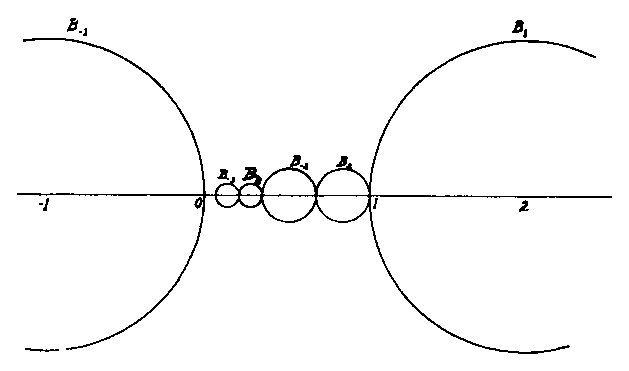
\includegraphics{chap04-vend-scan-03.eps}
\caption{Several streamlines (i.e. level curves of the stream
function) at a fixed time. The arrows represent the values of the
velocity field at this time at locations selected for
readability.}\label{ch04:fig3}
\end{figure}

Even though finite Fourier mode velocity fields are not strictly speaking homogeneous and isotropic, Figure~\ref{ch04:fig4} shows that the sample realizations of these velocity fields almost possess these properties. Also, note the similarities between the images of the modulus and the angle of the realization of the velocity field contained in Figure~\ref{ch04:fig4} with Figure 10 in \cite{ch04:bib34}.


\begin{figure}[!h]
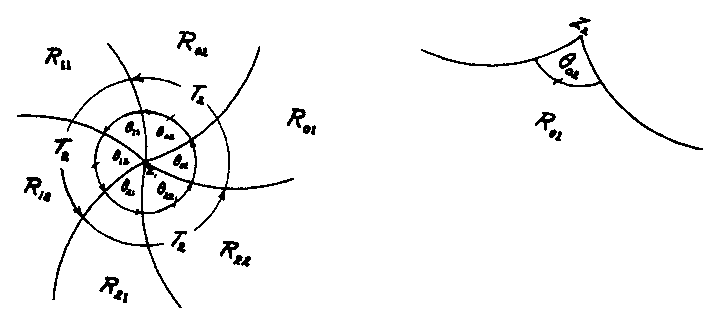
\includegraphics{chap04-vend-scan-04.eps} \caption{Left:
raster image of the length of $\vec{\mathbf{v}}(t,\,\cdot)$ taken
from a snapshot of a realization of the velocity field. Right:
raster image of the corresponding angle with a fixed direction. The
color code used to visualize the various directions is irrelevant at
this stage, we merely intend to illustrate the near homogeneity and
isotropy of the velocity field.}\label{ch04:fig4}
\end{figure}

The figures of this section have been taken from sequences of images produced to illustrate the time evolution of the realizations of the various scalar random fields (stream function, velocity modulus, velocity angle, $\cdot$). These images have been put together into animations which can be visualized with a web browser. They can be found at the URL \cite{ch04:bib18}. We find it extremely instructive to observe these time evolutions and we shall make a case based on evidence they produce when we discuss the Poisson models later in Section~\ref{ch04:sec7}. Unfortunately, a book chapter is not the appropriate medium for this type of illustration.

\subsection{Mean Square Error and Choice of the Parameters}\label{ch04:sec4.6} The estimation of the error is one of the many important theoretical problems which does not seem to have a satisfactory answer. If the goal is to understand the effects of the various approximations on the equation of motion and the transport properties of the flow, then the relevant quantity to control is:
\begin{equation}
\label{ch04:eqn4.23} \mathbb{E}\{\sup\limits_{0\leq t\leq T}\Vert\vec{\mathbf{v}}(t,\,\mathbf{x})-\vec{\mathbf{v}}_{\mathcal{K}}(t,\,\mathbf{x})\Vert^{2}\}
\end{equation}
where we use the notation $\vec{\mathbf{v}}_{\mathcal{K}}$ for the velocity field computed from the approximating stream function $\phi_{\mathcal{K}}$, whether the approximation is based on a wavelet\index{index}{wavelets} basis expansion or a Fourier expansion as described above. Unfortunately, because of the presence of the supremum inside the expectation, this error is difficult to estimate. On the other hand, the mean square error:
\begin{equation}
\label{ch04:eqn4.24} \mathbb{E}\{\Vert\vec{\mathbf{v}}(t,\,\mathbf{x})-\vec{\mathbf{v}}_{\mathcal{K}}(t,\,\mathbf{x})\Vert^{2}\}
\end{equation}
computed for a fixed (single) time $t$ is much easier to estimate, especially when the approximate decomposition is computed on an orthonormal system. This was done in the case of a time independent shear flow for an approximate decomposition in a wavelet basis both in \cite{ch04:bib26} and \cite{ch04:bib25}. A rough upper bound for (\ref{ch04:eqn4.24}) was derived in \cite{ch04:bib41} for an approximate decomposition using a discrete set $\mathcal{K}$ of Fourier modes. This bound was used to discuss the choice of the set $\mathcal{K}$. In particular it was argued that the set $\mathcal{K}$ should be chosen as a finite subset of a small set of concentric circles with radii in the inertial range $[r_{0},\,r_{1}]$. Moreover $\mathcal{K}$ should be chosen appropriately if the isotropy condition is desired, the optimal choices of the number of circles, of the values of the radii and of the numbers of wave vectors $\mathbf{k}$ per circle depending upon the values of the spectral parameters.

Unfortunately, the control of the mean square error (\ref{ch04:eqn4.24}) is of no use when we consider the large time properties of the flow. In particular, it is not sufficient to guarantee the convergence of the Lyapunov exponents of the (finite dimensional) approximate systems toward the Lyapunov exponent of the (infinite dimensional) full system. It is known that the approximation of Lyapunov exponents\index{index}{Lyapunov exponent!approximation} is already a touchy business in the case of ordinary stochastic differential equations (see for example \cite{ch04:bib44, ch04:bib32}) when the approximation is based merely on time discretization. The present situation is even more complex because of the approximation based on both time and space discretizations.

Besides, even though no one doubts the strict positivity of the upper Lyapunov exponent of the Jacobian flow in its full generality, no complete proof exists and the attempts based on the control of finite dimensional approximations have failed so far.

\section{Transport Simulations}\label{ch04:sec5}

We are concerned with the simulation of the trajectories of passive individual tracers as well as collective properties of the time evolution of sets of tracers. As explained in the introduction, the trajectories of the tracers are the solutions of the equation of motion:
\begin{equation}
\label{ch04:eqn5.1} dX_{t}=\vec{\mathbf{v}}(t,\,X_{t})dt+\sqrt{2\kappa}\,dW_{t},
\end{equation}
where $\{W_{t};\,t\geq 0\}$ is a Wiener process which is statistically independent of the velocity field $\vec{\mathbf{v}}$ and the constant $\kappa \geq 0$ represents the molecular diffusivity. For the sake of simplicity we shall assume that $\kappa =0$ when we discuss numerical simulations and we shall reinstall $\kappa$ (and hence the viscosity term) when we review the theoretical results on homogenization and more generally on transport renormalization. For each realization of the velocity field, the equation of motion is an ordinary differential equation and we denote by $\varphi_{s,t}$ the corresponding flow. The existence of such a flow is quite a difficult result in the presence of the Wiener process. It is one of the fundamental results of the modern theory of stochastic differential equations. See for example \cite{ch04:bib37}. In any case, $\varphi_{0,t}(\mathbf{x})$ is the solution $X_{t}$ of (\ref{ch04:eqn5.1}) with initial condition $X_{0}=\mathbf{x}$.

Once the choice of a sampling rate $\Delta t$ has been made, the positions of the tracer particles are computed at the times $t_{j}=t_{0}+j\Delta t$. In order to update the position of a particle one uses the simplest Euler scheme\index{index}{discretization!Euler scheme}:
\begin{equation}
\label{ch04:eqn5.2} \mathbf{x}(t_{j})=\mathbf{x}(t_{j-1})+\vec{\mathbf{v}}(t_{j},\,\mathbf{x}(t_{j-1}))\Delta t.
\end{equation}
Figure~\ref{ch04:fig6} shows a typical trajectory of a passive tracer. Using the notations introduced below, we used a set $\mathcal{K}$ of Fourier modes with 400 elements to simulate the values of the velocity field. These Fourier modes are plotted on figure~\ref{ch04:fig5}. The components of these Fourier modes and the values of the corresponding $\alpha$ and $\sigma$ parameters entering in the definitions of the scalar O-U processes are given by:
\begin{equation}
\label{ch04:eqn5.3} \alpha_{\mathbf{k}}=|\mathbf{k}|^{z}\quad \mathrm{and}\quad \sigma_{\mathbf{k}}=|\mathbf{k}|^{\frac{2-\epsilon}{2}}
\end{equation}\index{symbols}{$\alpha_{\mathbf{k}}$}\index{symbols}{$\alpha_{\mathbf{k}}$}
with $\epsilon=0.3$ and $z=1.2$.
\begin{figure}[!h]
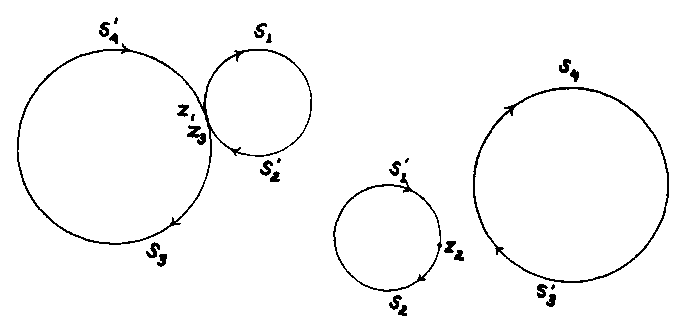
\includegraphics{chap04-vend-scan-05.eps}
\caption{Fourier modes used for the simulations.}\label{ch04:fig5}
\end{figure}

The values of the $\alpha$ and $\sigma$ parameters correspond to the values $\epsilon=1.8$ and $z=0.5$ of the spectral parameters of the model. The initial position $\mathbf{x}$ of the tracer shown in Figure~\ref{ch04:fig6} is the origin, the time increment is $\Delta t=0.01$ and we computed the position $\mathbf{x}(t_{j})$ for $J=120$ time samples $t_{j}$.

The simulation of the time evolution trajectories reduces to the problem of the generation of the velocity field, which in turn reduces to the generation of the stream function because of formula (4).

\subsection{Liquid Curves and Interface Fractalization}\label{ch04:sec5.1} The purpose of this section is to pursue the analysis initiated in \cite{ch04:bib12} of the time evolution of curves in the plane. All the results discussed below apply to general curves but for the sake of illustration we shall restrict ourselves to simple closed curves which we view as the boundaries of simply connected domains in the plane. They are called \emph{liquid curves} in \cite{ch04:bib34}.

Several authors have considered this problem in the case of Brownian flows where the analysis of the Lyapunov exponent is easier (see for example \cite{ch04:bib38, ch04:bib10, ch04:bib39, ch04:bib48}.) Results in the case of Ornstein Uhlenbeck velocity fields are reported in \cite{ch04:bib12} and \cite{ch04:bib14}. Mathematically speaking we are interested in the time evolution of a smooth curve:
\begin{equation*}
[0,1]\ni\alpha\hookrightarrow\gamma_{0}(\alpha)\in \mathbb{R}^{d}.
\end{equation*}
The latter can be viewed as the boundary at time $t=0$ of a cloud of pollutant dust particles which are light enough to be passively transported by the velocity field and we also assume that these dust particles do not interact. We analyze the time evolution of the shape of the cloud through the deformations over time of its boundary. We denote by $\gamma_{t}$\index{symbols}{$\gamma_{t}$} the boundary of the cloud at time $t$.

\begin{figure}[!h]
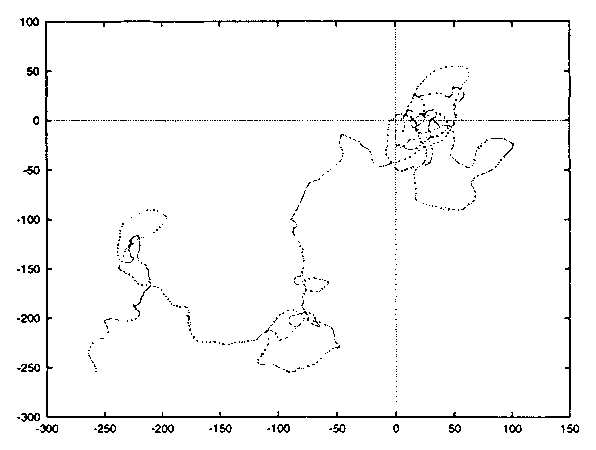
\includegraphics{chap04-vend-scan-06.eps}
\caption{Example of a passive tracer trajectory.}\label{ch04:fig6}
\end{figure}

\begin{equation*}
[0,\,1]\ni\alpha\hookrightarrow\gamma_{t}(\alpha)=\varphi_{0,t}(\gamma_{0}(\alpha))\in \mathbb{R}^{d}.
\end{equation*}
The results of the numerical simulations reported in \cite{ch04:bib13} (and reproduced in \cite{ch04:bib12}) confirmed what was known from the numerical simulations reported in \cite{ch04:bib34} and from proof existing in the case of Brownian flows: the length of $\gamma_{t}$ increases in all cases and the increase is more dramatic in the case of isotropic flows than in the case of shear flows. In fact it was shown in \cite{ch04:bib12} that the length of $\gamma_{t}$ is growing at most polynomially in the case of a shear flow and a simple argument was given to show that in general, the exponential rate of growth of the length of $\gamma_{t}$ is bounded from below by the Lyapunov exponent\index{index}{Lyapunov exponent} of the Jacobian flow. Also, numerical evidence was given for the strict positivity of this Lyapunov exponent in the case of flows with finitely many Fourier modes. This fact was subsequently proven in \cite{ch04:bib14}: the positivity of the Lyapunov exponent holds true as long as the Fourier modes are not concentrated on a line (i.e. as long as we are not dealing with a shear flow.)

Since the flow $\varphi_{s,t}$ is a flow of diffeomorphisms, the curve $\gamma_{t}$ remains smooth at all times, but as its length grows, its shape becomes very complex and intricate, filling up more and more space in the plane. After all, the length of $\gamma_{t}$ grows exponentially while its diameter grows only polynomially (presumably linearly as explained below in Subsection~\ref{ch04:sec5.2}.)

\begin{figure}[!h]
\includegraphics{chap04-vend-scan-07.eps}
\caption{Example of a time evolution of the unit
circle.}\label{ch04:fig7}
\end{figure}

\begin{figure}[!h]
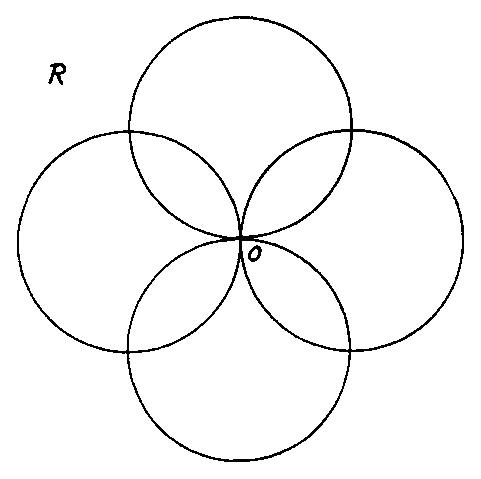
\includegraphics{chap04-vend-scan-08.eps}
\caption{Illustration of the mixing properties of the OU velocity
fields.}\label{ch04:fig8}
\end{figure}

Figure~\ref{ch04:fig7} shows a typical example of such a time evolution. The parameters of the velocity field were the same as before. From left to right and top to bottom the plots give the sets $\gamma_{t}$ for $t=0,\,19.2$, and $t=36$ for which we plotted the whole curve and a zoom on the central part. Notice that the circle is sampled with $N=500$ points at time $t=0$ and that, in order to keep the density constant along $\gamma_{t}$ we had to sample $\gamma_{t}$ with $N=500,\,N=17084$ and $N=954582$ at the instants $t=0\,t=16.8$ and $t=36$. Striking animations showing the time evolution of the curve $\gamma_{t}$ are given on the Web at the URL \cite{ch04:bib18}. The exponential increase of the length of $\gamma_{t}$ imposes on a corresponding exponential increase of the number of points to plot at each given time and this is the main limitation in the production of the animation files: memory capacity is reached very fast.

In any case, these numerical results suggest that the dimension of the subset of the plane formed by the points $\gamma_{t}(s)$ may, at least in an appropriate asymptotic regime, become strictly larger than 1.

Since there are many notions of fractal dimension, for the sake of simplicity, we concentrate on two specific choices. They are related to the Minkowski dimension and the so-called correlation dimension of $\gamma_{t}$.

We first discuss the Minkowski dimension. For each fixed time $t$ and each $\epsilon>0$ we compute the area $|\gamma_{t}(\epsilon)|$ of the sausage of width $\epsilon$ around $\gamma_{t}$ i.e. the area of the $\epsilon$ neighborhood:
\begin{equation*}
\gamma_{t}(\epsilon)=\{\mathbf{x};\,\exists\alpha\in[0,\,1],\,|\gamma_{t}(\alpha)-\mathbf{x}|\leq\epsilon\}
\end{equation*}
of the curve $\gamma_{t}$ and we look for a small $\epsilon$ asymptotic behavior of the form $|\gamma_{t}(\epsilon)|\approx C\epsilon^{d}$ so we could claim that the dimension of the curve is $d$. The existence of such an asymptotic behavior should be evidenced by a plot of the logarithm of $|\gamma_{t}(\epsilon)|$ versus the logarithm of $\epsilon$. Such a scatterplot should show that $|\gamma_{t}(\epsilon)|$ can be explained by a linear regression on $\epsilon$ and the Minkowski dimension should be given by the estimate of the slope. See Figure~\ref{ch04:fig9}. Because of the very intricate shape of the curve $\gamma_{t}$, the computation of the area $|\gamma_{t}(\epsilon)|$ could be problematic. We used a simple Monte Carlo simulation. We generated a large number of points in a rectangle containing the curve $\gamma_{t}$ with a uniform distribution and the area $|\gamma_{t}(\epsilon)|$ was approximated by the proportion of points within a distance $\epsilon$ of any of the points forming the curve $\gamma_{t}$.

We now explain the computation of the correlation dimension of $\gamma_{t}$, as proposed by Grassberger and Procaccia \cite{ch04:bib30, ch04:bib31} to characterize strange attractors. For each fixed time $t$ and each $\epsilon>0$ we consider
\begin{equation*}
C(\epsilon)=\frac{1}{N^{2}}\sum\limits_{i,j=1}^{N}1_{\{\Vert X_{i}-X_{j}\Vert<\epsilon\}}
\end{equation*}
where $N$ is the number of points of the discretized curve $\{X_{i},\,1\leq i\leq N\}$. $C(\epsilon)$ is expected to behave like $\epsilon^{\nu}$ for $\epsilon$ small, and $\nu$ is called the correlation dimension. As before we try to measure the small $\epsilon$ behavior of the logarithm of this number $C(\epsilon)$\index{symbols}{$C(\epsilon)$} as a function of the logarithm of $\epsilon$ and we derive an estimate of the dimension of $\gamma_{t}$ as before. Experiments carried out in \cite{ch04:bib30} on some strange attractors show that $\nu$ is a good estimate for the Hausdorff dimension.

Figure~\ref{ch04:fig9} shows numerical results attempting to determine the Minkowski and the correlation dimensions of $\gamma_{t}$ in the particular case of the unit circle $\gamma_{0}$ evolved under a velocity field with the same characteristics as above (section~\ref{ch04:sec5.3}).


\begin{figure}[!h]
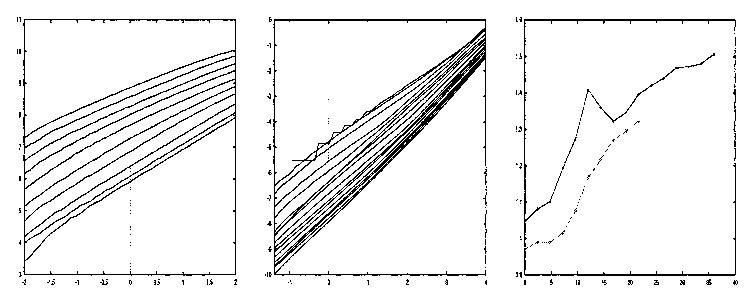
\includegraphics{chap04-vend-scan-09.eps}
\caption{Numerical evidence of the existence of an effective
(fractal) dimension. The Minkowski and the correlation exponents are
treated in the left and the middle plots respectively. The
estimations of the dimension by estimating the slopes are shown on
the right plot. The upper curve is related to the correlation
dimension.}\label{ch04:fig9}
\end{figure}

As explained earlier, the fractalization phenomenon is only a large time asymptotic effect. For each fixed finite $t>0$, the curve $\gamma_{t}$ is $C^{\infty}$ and consequently, the small $\epsilon$ behavior should be typical of a one-dimensional set, i.e. we should find a slope equal to 1 when we plot the logarithm of $N_{t}(\epsilon)$ versus the logarithm of $\epsilon$. In fact, when $\epsilon$ is too small for $t$, the zooming effect of $N_{t}(\epsilon)$ should show that $\gamma_{t}$ is a $C^{\infty}$ curve and the effective dimension should be 1. On the other hand, there should be an intermediate regime where $\epsilon$ is not small enough and $t$ is large enough to fool $N_{t}(\epsilon)$ into believing that it is dealing with a curve of dimension greater than 1. The numerical simulations reported in Figure~\ref{ch04:fig9} were intended to exhibit by varying both $\epsilon$ and $t$, this intermediate regime.

\begin{remark}\label{ch04:rem5.1}1. Related questions have been considered in \cite{ch04:bib7} where a slightly different problem involving the asymptotic dimension of interfaces was considered in a renormalization regime for time independent shear flows.

\noindent 2. Another interesting challenge is the numerical computation of the singularity spectrum of $\gamma_{t}$ in the multifractal formalism of \cite{ch04:bib11} and the analysis of its time evolution. We believe that an intermediate regime with fractal characteristics should be evidenced as we did above.

We also discuss a few conjectures for which we could not find numerical evidence (one way or another).
\end{remark}

\subsection{Diameter Asymptotics}\label{ch04:sec5.2} At time $t=0$ we consider a closed set $D_{0}$ and we consider its evolution under the flow. In other words we consider the time evolution of the random set $D_{t}=\varphi_{0,t}(D_{0})$. This subsection is concerned with the analysis of the diameter $d_{t}$ of this set. Notice that this diameter is equal to the diameter of the boundary $\partial D_{t}$ which in turn is the result of the transport by the flow of the boundary of the initial set $D_{0}$ since $\partial D_{t}=\varphi_{0,t}(\partial D_{0})$. In other words, we could start from $\partial D_{0}$ instead of $D_{0}$ without changing anything!

The goal is to find a (deterministic) function $t\hookrightarrow r_{t}$ for which:
\begin{equation*}
\lim\limits_{t\rightarrow\infty}\frac{d_{t}}{a_{t}}=1
\end{equation*}
almost surely, and possibly ''tests'' to determine upper and lower classes for this limit theorem. This problem is more difficult than it looks at first and no answer is known, even in the case of the Brownian flows. It is easy to show that:
\begin{equation*}
\lim\limits_{t\rightarrow\infty}\frac{d_{t}}{\sqrt{t}}=\infty
\end{equation*}
when the cardinality of $D_{0}$ is infinite, but the exact rate $a_{t}$ is elusive. The simplicity of the formulation of the problem is deceptive in the sense that it is not indicative of its difficulty. Y. Sinai (private conversation) suggested that $a_{t}$ could be a linear function of time. This conjecture is more or less explicit in \cite{ch04:bib34}. What is even more frustrating is that we were not able to set up simulations to validate (or invalidate) this conjecture. Indeed, any finite number of points of $D_{0}$ will escape at the diffusive rate of $\sqrt{t}$ and the rate $a_{t}$ can only be achieve by means of elongated fingers sticking out of $\partial D_{t}$ and surviving for a long time before being absorbed by the bulk of $D_{t}$, at which time new long finger will emerge. The sampling of the plane (and/or $\partial D_{t}$) would have to be refined in an adaptive way to illustrate such a phenomenon and we were not able to set up such simulations. This problem is one of the very many challenging questions which are left open.

\subsection{Mixing}\index{index}{mixing}\label{ch04:sec5.3} The asymptotic transport properties discussed in this chapter are strongly dependent upon the mixing properties of the flow. The latter have been studied in the case of Brownian flows in \cite{ch04:bib38}, \cite{ch04:bib10} and \cite{ch04:bib39} and it was shown there that the positivity of the upper Lyapunov exponent of the Jacobian flow was responsible for some of this mixing. Figure~\ref{ch04:fig8} illustrate the strong mixing properties of the Ornstein Uhlenbeck flows, even with a small number of Fourier modes as long as these modes are not aligned in the Fourier plane (recall that it was proven in \cite{ch04:bib14} that this condition guarantees the strict positivity of the Lyapunov exponent). The plots of The color plate Figure~\ref{ch04:fig8} was produced from flows generated by velocity fields of the type (\ref{ch04:eqn4.17}) and (\ref{ch04:eqn4.18}) with again the same parameters. Initially, we distribute the drifters (about 50, 000) uniformly in a square. We gave the same color to all the points contained in the same quadrant, and we plot the positions of these points over time (more precisely to times $t=0,\,t=48$ and $t=360$) with the same colors. The four colors being applied in a specific order by the printer (green, blue, red and finally yellow), the misleading impression that the numbers of points of the different colors are not the same, does result from this printing artifact. The plot on the bottom right was obtained by zooming in the central region of the plot on the bottom left.

\subsection{Upper Lyapunov Exponent of the Jacobian Flow}\label{ch04:sec5.4} As a final remark on the properties of the upper Lyapunov exponent of the Jacobian flow we mention the numerical analysis of the dependence of this exponent upon the spectral parameters $\epsilon$ and $z$ which was performed in \cite{ch04:bib12} using parallel computations on the MASPAR II. These numerical experiments suggest that this exponent is a smooth convex function of $\epsilon$ and $z$ but no rigorous result in this direction is known.

\section{Homogenization \& Spectral Singularity Renormalization}\index{index}{homogenization}
\label{ch04:sec6}

Physical systems with oscillating and/or random coefficients are difficult to analyze and many ad-hoc techniques have been proposed to average out the small scale variations of the coefficients and isolate the features of the solutions which are characteristics of scales larger than those of the typical variations of the coefficients. Among all the mathematical procedures designed to derive an effective equation governing the large time / large scale behavior of the solutions, homogenization\index{index}{homogenization} is certainly the most popular. In a nutshell, this procedure consists in studying the limit when the \emph{small parameter} $\delta$ tends to 0 of the solutions after the rescalings
\begin{equation}
\label{ch04:eqn6.1} t\rightarrow t/\delta^{2}\qquad \mathrm{and}\qquad \mathbf{x}\rightarrow \mathbf{x}/\delta
\end{equation}
of the time and the space variables. It can be applied to \emph{ordinary} (stochastic) differential equations such as the equation of motion as well as to (stochastic) partial differential equations such as the stochastic parabolic equation of the concentrations of passive tracers.

Because this problem has been thoroughly investigated, the literature on the subject is enormous. Most of the published works concern the time independent case. We shall only quote the lecture notes \cite{ch04:bib43} for the probabilistic approach and \cite{ch04:bib7} for a more analytic perspective. Both are well suited for the type of equations considered here and we suggest to the interested reader to consult the many references therein.

For the time dependent case we refer to \cite{ch04:bib16} and to the references therein. The proof of \cite{ch04:bib16} is different from most of the proofs in the time independent case in that it takes full advantage of the Markov property of the Eulerian velocity field. The main thrust of this proof is to identify the distribution of the Lagrangian motions and to analyze its ergodic properties. This proof was originally restricted to the finite Fourier mode case. It has been extended to the general case in \cite{ch04:bib17}. One of its interesting characteristics is that it does not rely on the assumption $\kappa >0$ and according to \cite{ch04:bib34}, no rigorous proof was known that this assumption could be dispensed with.

In its strongest probabilistic formulation homogenization can be viewed as a functional central limit theorem for the rescaled solutions of the equation of motion and the result states that in the large time / large scale regime given by the diffusive scaling (\ref{ch04:eqn6.1}) the Lagrangian motions are essentially Brownian motions with a variance, the so-called effective diffusivity, which is a complicated function of the original diffusivity constant\index{index}{diffusivity constant} $\kappa$ and the spectral parameters of the model. As explained above this result was proved in \cite{ch04:bib16} for the finite Fourier mode models and we believed at that time that the result should hold in full generality as long as there is no infrared spectral singularity. In fact we proved in \cite{ch04:bib17} that it is valid for general O-U models as long as:
\begin{equation}
\label{ch04:eqn6.2} \epsilon+z<2.
\end{equation}
This result was proved by Avellaneda and Majda in \cite{ch04:bib6} for the shear flow models. In their path-breaking analysis of the shear flow models these authors showed that depending on the nature of the spectral singularity (more precisely depending on which region of the $(\epsilon,\,z)$-plane of spectral parameters the couple $(\epsilon,\,z)$ belongs to) it is possible to find a large time / large scale rescaling
\begin{equation}
\label{ch04:eqn6.3} t\rightarrow t/\rho(\delta)^{2}\qquad \mathrm{and}\qquad \mathbf{x}\rightarrow \mathbf{x}/\delta
\end{equation}
for which the solutions of the rescaled parabolic equation for the concentrations converges to the solution of a limiting equation. According to these results, in each region of the spectral parameter plane, the nature of the time scaling $\rho(\delta)$ and the nature of the limiting equation give a sub-diffusive, diffusive or super-diffusive large time / large scale motion. This partition of the $(\epsilon,\,z)$ plane identified in \cite{ch04:bib6} for shear flow models was claimed to be universal. Attempts have been made in \cite{ch04:bib17} to show what remains of this partition in the general case but the results remain speculative and partial at best.

A different set of renormalization procedures was proposed in \cite{ch04:bib28} for the same shear flow models studied in \cite{ch04:bib6}. A heated debate followed the publication of \cite{ch04:bib23} and the controversy remains mostly unresolved.

The results of the renormalization procedures are striking mathematical properties of the asymptotics of the models. Our experience is that they are extremely difficult if not impossible to illustrate numerically.

As we already pointed out, the computation of the structure function requires the evaluation of the velocity field at one (single) point\index{index}{Poisson!point processes} in space which does not change with time or the realization of the velocity field. Moreover this computation does not see much of the spectral singularity. It is conceivable that computations of this type are feasible, especially in the time-independent case. Computations of the structure function are described in \cite{ch04:bib26} where the authors use wavelet\index{index}{wavelets} - like expansions to confirm numerically some of the theoretical findings of the renormalization theory of time independent shear flows. We were able to reproduce these results with Fourier - like expansions but because the use of wavelets is well adapted to the approach to the singularity, at equal approximation error, the computational burden of the Fourier - like expansions is bigger. A similar wavelet - like expansion was used in \cite{ch04:bib25} to compute numerically the mean square displacement $\mathbb{E}\{||\varphi_{0,t}(\mathbf{x}_{1})-\varphi_{0,t}(\mathbf{x}_{2})||^{2}\}$ as a function of the time $t$ and the initial separation $||\mathbf{x}_{1}-\mathbf{x}_{2}||$ of the starting points of the Lagrangian trajectories. These computations can be done explicitly in the case of time independent shear flow. The authors use the numerical computation of this mean square displacement by Monte Carlo simulation\index{index}{homogenization!simulations} of the velocity field and solution of the equation of motion as a test for the method chosen to simulate the velocity field. These simulations are of the transport type but, because the authors of \cite{ch04:bib25} are using a time independent shear flow model, given the knowledge of $t$ and $\Vert \mathbf{x}_{1}-\mathbf{x}_{2}\Vert$, the points at which the velocity will have to be computed form a deterministic (linear) set which can be computed up-front. With this knowledge it become easy to determine which wavelet coefficients will be needed and which Gaussian random variables need to be generated in order to set up the simulation. This is not possible in the general case of a \emph{non shear flow} model for which one cannot predict with certainty where the velocity field will have to be computed. As we explained earlier in Subsection~\ref{ch04:sec4.3} the number of Gaussian random variables to generate and the number of wavelet coefficients to compute are so big that the computations become prohibitive, especially in the time-dependent case.

Notice also that simulations attempting to illustrate the homogenization regime are reported in \cite{ch04:bib34}, but no means is provided to assess the nature of the approximations and to quantify the corresponding errors.

We believe that the numerical analysis of the renormalization limits of the transport properties of singular velocity fields of a general nature is beyond the scope of the current computer and mathematical technology.

\section{Poisson Models}\label{ch04:sec7}

Gaussian fields are not the only models of stationary and homogeneous random velocity fields which have been studied for their transport properties. A popular model consists in the linear superposition of elementary localized velocity fields scattered in space as a Poisson point process. These elementary velocity fields are chosen to mimic the behavior of vortices. These vortices do not interact and are not transported by the flow, so these models are different from the computational algorithms proposed by Chorin to compute numerically solutions of the 2-D Navier Stokes equation \cite{ch04:bib20}. A time independent model of this type has been considered in \cite{ch04:bib8} but we shall concentrate our discussion on the time dependent case of shot noise velocity fields introduced by Cinlar in \cite{ch04:bib21} and \cite{ch04:bib22}. The ''\emph{O-U nature}'' of these models makes us believe that the results presented here for O-U velocity fields with Gaussian statistics should still hold for these shot noise Poisson velocity fields. We even believe that the strong mixing properties (consequences of the uniform spectral gap and in particular the lack of infrared spectral singularity) of the velocity field introduced in \cite{ch04:bib21} and \cite{ch04:bib22} should make some of the proofs (positivity of the upper Lyapunov of the Jacobian flow, homogenization\index{index}{homogenization}, $\ldots$) easier. But these claims are mere speculations since we do not know of any proof of these results.

There is no doubt in our mind that the shot noise Poisson models form a class of interesting mathematical models which deserve to be studied for their own sake. But we would like to re-battle one of the common arguments used to justify their introduction: ``\emph{they possess vorticity\index{index}{velocity field!vorticity} features which cannot be produced by the Gaussian models}''. In fact, the theory of extremes of random fields tells us that the very high peaks of a homogeneous Gaussian stream function form (at least asymptotically) a Poisson process in the plane. See for example \cite{ch04:bib1}. Moreover, as we saw from Figure~\ref{ch04:fig3} each peak produces a vortex and if a peak remains a peak for a significant amount of time, this vortex will create a spinning motion of the passive tracers up until the peak of the stream function is absorbed. This phenomenon is quite obvious from the animations available on the Web page \cite{ch04:bib18}. We are convinced that these long lived vortices do exists in Gaussian models and one may legitimately ask :
\begin{quote}
why create artificially and by brute force features which are already
present in the Gaussian models?
\end{quote}
\emph{Acknowledgments: The first named author (RC) would like to thank Jean Pierre Fouque for pointing out the review article \emph{\cite{ch04:bib34}} of Isichenko. The second named author (FC) would like to thank the Department of Civil Engineering \& Operations Research of Princeton University for its warm hospitality and the Office of Naval Research for partially supporting the visits during which most of this work was done.}

\begin{thebibliography}{48}
\bibitem{ch04:bib1} R.J. Adler (1980): Geometry of Random Fields. Wiley, New York, N.Y.

\bibitem{ch04:bib2} K.S. Alexander (1996): Boundedness of level lines for two-dimensional random fields. \emph{Ann. Probab}. \textbf{24}, 1653 - 1674.

\bibitem{ch04:bib3} K.S. Alexander and S.A. Molchanov (1994): Percolation of level sets for two dimensional random fields with lattice symmetry. \emph{J. Stat. Phys}. \textbf{77}, 627 - 643.

\bibitem{ch04:bib4} A. Antoniadis and R. Carmona (1985): Infinite Dimensional Ornstein Ulhenbeck Processes \emph{Probab. Th. Rel. Fields} \textbf{74}, 31-54.

\bibitem{ch04:bib5} M. Avellaneda, F. Elliott and A. Appelian (1993): Trapping, Percolation and Anomalous Diffusion of Particles in a Two-Dimensional Random Field. \emph{Journal of Statistical Physics} \textbf{72}, 1227-1304.

\bibitem{ch04:bib6} M. Avellaneda and A. Majda (1990): Mathematical models with exact renormalization for turbulent transport. \emph{Commun. Math. Phys}., \textbf{131}, 381-429.

\bibitem{ch04:bib7} M. Avellaneda and A. Majda (1990): Mathematical Models with Exact Renormalization for Turbulent Transport. \emph{Commun. Math. Phys}., \textbf{131}, 381-429.

\bibitem{ch04:bib8} M. Avellaneda and S. Torquato (1991): Diffusion and Geometric Effects in Passive Advection by Random Arrays of Vortices. \emph{Phys. Fluids A}, \textbf{3}, 1880-1891.

\bibitem{ch04:bib9} G.K. Batchelor (1982): The theory of homogeneous turbulence. \emph{Cambridge University Press}, Cambridge.

\bibitem{ch04:bib10} P.H. Baxendale (1986): Asymptotic Behavior of Stochastic Flows of Diffeomorphisms: Two Case Studies. \emph{Proba. Th. Rel. Fields} \textbf{73}, 51-85.

\bibitem{ch04:bib11} J.F. Buzy, E. Bacry and A. Arneodo (1992): Multifractal formalism for fractal signals: the structure function approach versus the wavelet transform modulus maxima method. (preprint)

\bibitem{ch04:bib12} R. Carmona (1996): Transport Properties of Gaussian Velocity Fields, \emph{in Real and Stochastic Analysis}: \emph{Recent Advances} ed. M.M. Rao, CRC Press

\bibitem{ch04:bib13} R. Carmona, S. Grishin and S.A. Molchanov (1994): Massively Parallel Simulations of the Transport Properties of Gaussian Velocity Fields, to appear in \emph{Mathematical Models for Oceanography}, eds R. Adler, P. Muller and B. Rozovskii. Birkha\"{u}ser.

\bibitem{ch04:bib14} R. Carmona, S. Grishin, S.A. Molchanov and L. Xu (1995): Exponential Stretching for Ornstein Ulhenbeck Flows with Finitely Many Frequency Modes. \emph{Electr. Comm. Probab}. (to appear).

\bibitem{ch04:bib15} R. Carmona and A. Wang (1994): Comparison Tests for the Spectra of Dependent Multivariate Time Series, in \emph{Mathematical Models for Oceanography}, eds R. Adler, P. Muller and B. Rozovskii. Birkha\"{u}ser.

\bibitem{ch04:bib16} R. Carmona and L. Xu (1997): Homogenization for Time Dependent 2-D Incompressible Gaussian Flows. \emph{Ann. Appl. Probab}. (to appear)

\bibitem{ch04:bib17} R. Carmona and L. Xu (1997): Renormalization Results for Time Dependent Incompressible OU Velocity Fields, (in preparation)

\bibitem{ch04:bib18} URL \texttt{http://chelsea.princeton.edu/$^{\sim}$ rcarmona/simul/transport.html}

\bibitem{ch04:bib19} URL \texttt{http://soil.princeton.edu/$^{\sim}$rcarmona/researchinterests.html}

\bibitem{ch04:bib20} A.J. Chorin (1994): Vorticity and Turbulence. Springer Verlag, New York, N.Y.

\bibitem{ch04:bib21} E. Cinlar (1994): On a Stochastic Velocity Field, (preprint)

\bibitem{ch04:bib22} E. Cinlar (1994): Poisson Shot Noise Velocity Fields, (preprint)

\bibitem{ch04:bib23} E. Cinlar and C.L. Zirbel (1996): Dispersion of Particle Systems in Brownian Flows. \emph{Adv. Appl. Probab}. \textbf{28}, 53-74.

\bibitem{ch04:bib24} I. Daubechies (1992): Ten Lectures on Wavelets. SIAM

\bibitem{ch04:bib25} F. Elliott, D. Horntrop and, A. Majda (1996): A Fourier - Wavelet Monte Carlo Method for Fractal Random Fields, (preprint)

\bibitem{ch04:bib26} F. Elliott and A. Majda (1994): A Wavelet Monte Carlo Method for Turbulent Diffusion with Many Spatial Scales. \emph{J. Comput. Phys}. \textbf{113}, 82-111.

\bibitem{ch04:bib27} J. Gaines (1995): Numerical Experiments with S(P)DE's. \emph{in Stochastic Partial Differential Equations} ed. A. Etheridge. London Math. Soc. Lect. Note Series \textbf{216}, Cambridge Univ. Press.

\bibitem{ch04:bib28} J. Glimm and Q. Zhang (1992): Inertial Range Scaling of Laminar Shear Flow as a Model of Turbulent Transport. \emph{Commun. Math. Phys}., \textbf{146}, 217-229.

\bibitem{ch04:bib29} S. Grishin (1997): PhD CEOR, Princeton University

\bibitem{ch04:bib30} P. Grassberger and I. Procaccia (1983): Characterization of Strange Attractors. \emph{Phys. Rev. Lett}. \textbf{50}(5), 346-349.

\bibitem{ch04:bib31} P. Grassberger and I. Procaccia (1983): Estimation of the Kolmogorov Entropy from a Chaotic Signal. \emph{Phys. Rev. A} \textbf{28}(4), 2591-2593.

\bibitem{ch04:bib32} A. Grorud and D. Talay (1995): Approximation of Upper Lyapunov Exponents of Bilinear Stochastic Differential Systems. \emph{SIAM J. Numer. Anal}. \textbf{28}(4), 1141-1164.

\bibitem{ch04:bib33} D.J. Horntrop and A.J. Majda (1994): Subtle Statistical Behavior in Simple Models for Random Advection-Diffusion. \emph{J. Math. Sci. Univ. Tokyo} \textbf{1}, 23-70.

\bibitem{ch04:bib34} M.B. Isichenko (1992): Percolation, statistical topography and transport in random media. \emph{Rev. Modern Phys}. \textbf{64}, 961-1043.

\bibitem{ch04:bib35} R.M. Kraichnan (1959): The structure of isotropic turbulence at very high Reynolds numbers. \emph{J. Fluids Mech}. \textbf{5}, 497-543.

\bibitem{ch04:bib36} R.M. Kraichnan (1974): Convection of a passive scalar by a quasi uniform random straining field. \emph{J. Fluids Mech}. \textbf{64}, 737-762.

\bibitem{ch04:bib37} H. Kunita (1990): Stochastic Flows and Differential Equations. Cambridge University Press.

\bibitem{ch04:bib38} Y. Le Jan (1984): On isotropic Brownian motions. \emph{Z. Wahrscheinlichkeitstheorie verw. Geb}. \textbf{70}, 609-620.

\bibitem{ch04:bib39} Y. Le Jan (1991): Asymptotic Properties of Isotropic Brownian Flows. \emph{in Spatial Stochastic Processes}, eds K.S. Alexander, J.C. Watkins, pp 219-232, Birkha\"{u}ser, Boston.

\bibitem{ch04:bib40} A.J. Majda (1994): Random Shearing Direction Model for Isotropic Turbulent Diffusion. \emph{J. Statist. Phys}. \textbf{75}, 1153-1165.

\bibitem{ch04:bib41} S.A. Molchanov (1994): Topics in Statistical Oceanography, in \emph{Mathematical Models for Oceanography},pp. 343-380, eds R. Adler, P. Muller and B. Rozovskii. Birkha\"{u}ser.

\bibitem{ch04:bib42} A.S. Monin and A.M. Yaglom (1971): Statistical Fluid Mechanics: Mechanics of Turbulence. MIT Press, Cambridge, Mass.

\bibitem{ch04:bib43} S. Olla (1994): Homogenization of Diffusion Processes in Random Fields, (preprint, Ecole Polytechnique Paris.)

\bibitem{ch04:bib44} D. Talay (1991): Lyapunov Exponents of Nonlinear Stochastic Differential Equations. \emph{SIAM J. Appl. Mat}. (to appear).

\bibitem{ch04:bib45} G.I. Taylor (1953): Dispersion of Soluble Matter in Solvent flowing Slowly through a Tube. \emph{Proc. Royal Soc. A} \textbf{219}, 186-203.

\bibitem{ch04:bib46} J.B. Walsh (1986): An Introduction to Stochastic Partial Differential Equations in \emph{Ecole d'Et\'{e} de Probabilit\'{e}s de Saint Flour 1984} Lect. Note in Math. \textbf{1180}, 265-439.

\bibitem{ch04:bib47} A.M. Yaglom (1987): Correlation Theory of Stationary and Related Random Functions, vol. I: Basic Results. Springer Verlag, New York, N.Y.

\bibitem{ch04:bib48} C.L. Zirbel (1993): Stochastic Flows: Dispersion of a Mass Distribution and Lagrangian Observations of a Random Field. Ph. D. Princeton.
\end{thebibliography}

%%%%%%%%%%%chapter05
\part{MATHEMATICAL THEORY\label{pt02:part02a}}

\chapter{An analytic approach to SPDEs\label{ch05:chap05}}

\begin{flushright}
\hfill{N.V. KRYLOV}\\
\hfill{127 Vincent Hall}\\
\hfill{University of Minnesota}\\
\hfill{Minneapolis, MN, 55455}\\
\hfill{\texttt{\textbf{krylov@math.umn.edu}}}
\end{flushright}

\section{Introduction}
\label{ch05:sec1}

Evolutional stochastic partial differential equations (SPDEs) arise in many applications of probability theory and have been treated since long ago (see \cite{ch05:bib30}). An example of a linear second-order SPDE is given by the following equation in $\mathbb{R}^{d}$:
\begin{equation}
\label{ch05:eqn1.1} du=(a^{ij}u_{x^{i}x^{j}}+b^{i}u_{x^{i}}+cu+f)\,dt+(\sigma^{ik}u_{x^{i}}+\nu^{k}u+g^{k})\,dw_{t}^{k},\
t>0,
\end{equation}
where summation with respect to the repeated indices $i,\,j,\,k$ is assumed as usual, $i$ and $j$ go from 1 to $d$, and $k$ may run through 1, 2, $\ldots$.

The main purpose of this publication is to present a theory of solvability of the Cauchy problem for linear and some quasi-linear equations like (\ref{ch05:eqn1.1}) in spaces of summable functions with exponent of summability $p\geq 2$. If $p=2$, so that we are concerned with solutions belonging to the Sobolev spaces $W_{2}^{n}(\mathbb{R}^{d})$\index{symbols}{$W_{2}^{n}(\mathbb{R}^{d})$}, such a theory does exist and is rather complete and satisfactory (see, for instance, \cite{ch05:bib30}). Recall that $W_{2}^{n}(\mathbb{R}^{d})$ is the set of all generalized functions on $\mathbb{R}^{d}$ whose derivatives up to and including the $n$th order belong to $L_{2}(\mathbb{R}^{d})$. Some results concerning the solvability of the first boundary-value problem in spaces like $W_{2}^{n}(D)$, where $D$ is a smooth domain, can be found in \cite{ch05:bib02}, \cite{ch05:bib06}, \cite{ch05:bib20}, and \cite{ch05:bib32}. Roughly speaking, the main tool in $W_{2}^{n}$-theory is integration by parts. There are also approaches based on semigroup methods \cite{ch05:bib05}, \cite{ch05:bib06}, which work well for the equations with nonrandom leading coefficients $a^{ij}$ and again in the Hilbert-space framework.

The necessity of the $L_{p}$--theory arises, for instance, when one wants to find the solutions numerically. The convergence rate and the way the finite difference should be chosen depend on smoothness properties of solutions. Here by the smoothness properties we mean continuity, H\"{o}lder continuity, differentiability, continuity of derivatives, and so on.

One of inconveniences of $W_{2}^{n}$-theory is that $W_{2}^{n}(\mathbb{R}^{d})\subset \mathcal{C}^{n-d/2}(\mathbb{R}^{d})$ only if $2n>d$, and one can prove that the solutions belong to $W_{2}^{n}(\mathbb{R}^{d})$ only if the coefficients are $n-2$ times continuously differentiable. Therefore, if we want to get the solutions $m$ times continuously differentiable with respect to $x\in
\mathbb{R}^{d}$, we have to suppose that the coefficients of the equation are more than $m+d/2-2$ times continuously differentiable even if the free terms are of class $C_{0}^{\infty}(\mathbb{R}^{d})$. At the same time, $W_{p}^{n}(\mathbb{R}^{d})\subset \mathcal{C}^{n-d/p}(\mathbb{R}^{d})$ if $pn>d$, and, by taking $p$ sufficiently large, we see that the solutions have almost as many usual derivatives as generalized ones. Actually, exactly for this purpose the spaces $W_{p}^{n}(\mathbb{R}^{d})$ with $p\geq 2$ have already been used in SPDE theory (see, for instance, \cite{ch05:bib30}), but the corresponding results, obtained again by integration by parts, were not sharp. It is worth mentioning that sharp results concerning $\mathcal{C}^{2+\alpha}(\mathbb{R}^{d})$--theory are recently obtained in \cite{ch05:bib27} for equations like (\ref{ch05:eqn1.1}) but with $\sigma \equiv 0$.

Another advantage of the $W_{p}^{n}$ setting with $p\geq 2$ can be seen in the case of very popular equations with so-called cylindrical white noise (see, for instance, \cite{ch05:bib08}, \cite{ch05:bib26}, \cite{ch05:bib28}, \cite{ch05:bib35}, and references therein). Although these equations are covered by the general $W_{p}^{n}$-theory for any $p\geq 2$ (see Section~\ref{ch05:sec8.3}), for $p=2$ we get only the solutions summable to any degree, and the solutions become continuous only for $p>2$. By the way, as in \cite{ch05:bib30}, we consider $n$ positive and negative, but in contrast with \cite{ch05:bib30} we allow $n$ to have non-integer values. For general $n$ we are working in the spaces of Bessel potentials $H_{p}^{n}(\mathbb{R}^{d})$\index{symbols}{$H_{p}^{n}(\mathbb{R}^{d})$}, and, in the case of equations with cylindrical white noise, we take $n$ slightly less than $(-3/2)$.

Our main tool is the theory of spaces $H_{p}^{n}(\mathbb{R}^{d})$, borrowed from \cite{ch05:bib33}, together with a result from \cite{ch05:bib17} or \cite{ch05:bib18} which is an analog of the so-called maximal regularity property of stochastic convolutions in Hilbert spaces obtained by Da Prato (cf. \cite{ch05:bib04}). We also use some results from the theory of parabolic equations and follow a general scheme of proving the solvability of PDEs adopted in this theory. We discuss this general scheme in Sec.~\ref{ch05:sec2}.

The main source of these notes is author's article \cite{ch05:bib20}. However, it underwent a major revision and restructuring here, so that, in author's opinion, the whole subject looks more natural now. Also, the proofs are given with much more details, and several mistakes have been corrected. In this regard the contribution of S. Lototsky, H. Yoo, and A. Zatezalo is greatly appreciated. The author has delivered four lectures on the subject at Workshop/School on SPDEs, Theory and Applications, Los Angeles, January, 3--7, 1996. This was a very good opportunity to think all over again. It is a pleasure to thank the organizers of the Workshop for the invitation and hospitality.

\section{Generalities}
\label{ch05:sec2}

We want to explain here some basic ideas guiding the investigation we are going to present further.

Rewrite equation (\ref{ch05:eqn1.1}) in the following form
\begin{equation}
\label{ch05:eqn2.1} du=(Lu+f)\,dt+(\Lambda^{k}u+g^{k})\,dw_{t}^{k},\ t>0,
\end{equation}\index{symbols}{$Lu$}\index{symbols}{$\Lambda u$}
where
\begin{equation*}
Lu=a^{ij}u_{x^{i}x^{j}}+b^{i}u_{x^{i}}+cu,\quad \Lambda^{k}u\,=\sigma^{ik}u_{x^{i}}+\nu^{k}u.
\end{equation*}
Recall that we are using the summation convention. Of course, $w_{t}^{k}$\index{symbols}{$w_{t}^{k}$} are independent Wiener processes and $du$ is It\^{o}'s stochastic differential with respect to $t$. The equation is considered for all $x\in \mathbb{R}^{d}$ and $t>0$. The coefficients $\sigma,\,\nu$, and the ``free'' term $g$ may vanish, and then (\ref{ch05:eqn2.1}) becomes a usual parabolic partial differential equation. Therefore, it is natural to recall some ideas and results from the $L_{p}$-theory of parabolic partial differential equations.

Let $\mathbb{R}^{d}$\index{symbols}{$\mathbb{R}^{d}$} be a $d$-dimensional Euclidean space of points $x= (x^{1}, \ldots, x^{d})$. By a distribution or a generalized function on $\mathbb{R}^{d}$ we mean an element of the space $\mathcal{D}$\index{symbols}{$\mathcal{D}$} of real-valued Schwarz distributions defined on $C_{0}^{\infty}$\index{symbols}{$C_{0}^{\infty}$}, where $C_{0}^{\infty}=C_{0}^{\infty}(\mathbb{R}^{d})$ is the set of all infinitely differentiable functions with compact support.

For given $p\in(1, \infty)$ and $n\in(-\infty, \infty)$, define the space $H_{p}^{n}=H_{p}^{n}(\mathbb{R}^{d})$ (called the space of Bessel potentials or the Sobolev space with fractional derivatives) as the space of all generalized functions $u$ such that $(1-\Delta)^{n/2}u\in L_{p}=L_{p}(\mathbb{R}^{d})$. To explain the meaning of this, let us first introduce $(1-\Delta)^{n/2}$\index{symbols}{$(1-\Delta)^{n/2}$} in the following way (see \cite{ch05:bib14}). If $\alpha\in(0,1)$, then, for a constant $c(\alpha)$ and all $z\leq 0$,
\begin{equation*}
(1-z)^{\alpha}=c(\alpha)\int_{0}^{\infty}\frac{e^{-t}e^{zt}-1}{t^{\alpha}}\frac{dt}{t}.
\end{equation*}
If we formally substitute here $\Delta$ instead of $z$, then we get the following definition of $(1-\Delta)^{\alpha}$
\begin{equation}
\label{ch05:eqn2.2} (1-\Delta)^{\alpha}u=c(\alpha)\int_{0}^{\infty}\frac{e^{-t}T_{t}u-u}{t^{\alpha}}\frac{dt}{t},
\end{equation}
where $T_{t}$\index{symbols}{$T_{t}$} is the semigroup associated with $\Delta$, that is, a solution of $T_{t}^{\prime}=\Delta T_{t}$ similarly to $e^{zt}$ which is a solution of $f^{\prime}=zf$. The following is an explicit formula for $T_{t}$:
\begin{equation}
\label{ch05:eqn2.3} T_{t}u(x):=\frac{1}{(4\pi t)^{d/2}}\int_{\mathbb{R}^{d}}u(y)e^{-\frac{1}{4t}|x-y|^{2}}\,dy.
\end{equation}
In the same way for any $\alpha>0$ we define
\begin{equation}
\label{ch05:eqn2.4} (1-\Delta)^{-\alpha}u=d(\alpha)\int_{0}^{\infty}t^{\alpha}e^{-t}T_{t}u\frac{dt}{t},
\end{equation}
where $d(\alpha)$ is an appropriate constant. It turns out (see \cite{ch05:bib14}) that formulas (\ref{ch05:eqn2.2}) and (\ref{ch05:eqn2.4}) are sufficient to consistently define $(1-\Delta)^{n/2}$ for any $n\in\,(-\infty, \infty)$. The result of application of $(1-\Delta)^{-n/2}$ to an $f\in L_{p}$ is defined as a limit of truncated integrals in (\ref{ch05:eqn2.2}) or (\ref{ch05:eqn2.4}). For a distribution $u$, we say that $u\in H_{p}^{n}$ if there is $f\in L_{p}$ such that $u=(1-\Delta)^{-n/2}f$ in the sense of distributions, that is, if $u$ and $(1-\Delta)^{-n/2}f$ coincide as elements in the space $\mathcal{D}$. In this case we also write $(1-\Delta)^{n/2}u=f$.

For $u\in H_{p}^{n}$ one introduces the norm
\begin{equation*}
\Vert u\Vert_{n,p}:=\Vert (1-\Delta)^{n/2}u\Vert_{p},
\end{equation*}
where $\Vert\,\cdot\,\Vert_{p}$\index{symbols}{$\Vert\,\cdot\,\Vert_{p}$} is the norm in $L_{p}$\index{symbols}{$L_{p}$}. It is known (see, for instance, \cite{ch05:bib33}, \cite{ch05:bib34}) that $H_{p}^{n}$\index{symbols}{$H_{p}^{n}$} is a Banach space with norm $\Vert\,\cdot\,\Vert _{n,p}$\index{symbols}{$\Vert\,\cdot\,\Vert_{n,p}$} and the set $C_{0}^{\infty}$ is dense in $H_{p}^{n}$.

Next, for fixed $T$ one introduces the space $H_{p}^{1,2}(T)=H_{p}^{1,2}((0,T)\times \mathbb{R}^{d})$ as
\begin{equation*}
\{u=u(t,x):\Vert u\Vert_{1,2,p}^{p}:=\int_{0}^{T}\Vert \frac{\partial u}{\partial t}(t,\cdot)\Vert_{p}^{p}\,dt+\int_{0}^{T}\Vert u(t,\cdot)\Vert_{2,p}^{p}\,dt<\infty\}.
\end{equation*}
The norm $\Vert\,\cdot\,\Vert_{1,2,p}$\index{symbols}{$\Vert\,\cdot\,\Vert_{1,2,p}$} makes $H_{p}^{1,2}(T)$\index{symbols}{$H_{p}^{1,2}(T)$} a Banach space.

The investigation of the deterministic counterpart of equation (\ref{ch05:eqn2.1})
\begin{equation}
\label{ch05:eqn2.5} \frac{\partial u}{\partial t}=Lu+f
\end{equation}
with zero initial condition goes in the following way (see \cite{ch05:bib31}). First, for the simplest equation
\begin{equation}
\label{ch05:eqn2.6} \frac{\partial u}{\partial t}=\Delta u+f,
\end{equation}
its solvability in $H_{p}^{1,2}(T)$ is proved by means of explicit formulas and some estimates of heat potentials, provided that $f\in L_{p}\,((0,T)\times \mathbb{R}^{d})$. In Subsec.~\ref{ch05:sec4.1} we use the following theorem which is proved in \cite{ch05:bib31} (also see Remark 2.3.2 in \cite{ch05:bib34}).

\begin{theorem}\label{ch05:thm2.1}
For any $f\in L_{p}\,((0,T)\times \mathbb{R}^{d})$ and $u_{0}\in H_{p}^{2-2/p}$ there exists a unique solution $u\in H_{p}^{1,2}(T)$ of the heat equation (\ref{ch05:eqn2.6}) with initial data $u(0)=u_{0}$. In addition,
\begin{gather}\label{ch05:eqn2.7}
\Vert u_{xx}\Vert_{L_{p}((0,T)\times \mathbb{R}^{d})}+\Vert \frac{\partial u}{\partial t}\Vert_{L_{p}((0,T)\times \mathbb{R}^{d})}\leq N(d,p)(\Vert f\Vert _{L_{p}((0,T)\times \mathbb{R}^{d})}+\Vert u_{0}\Vert _{2-2/p,p}),\\
\quad \Vert u\Vert _{1,2,p}\leq N(d,p,T)(\Vert f\Vert _{L_{p}((0,T)\times \mathbb{R}^{d})}+\Vert u_{0}\Vert _{2-2/p,p}),\nonumber
\end{gather}
where $u_{xx}$ is the matrix of second--order derivatives of $u$ with respect to $x$.
\end{theorem}

This theorem yields a bounded operator $\mathcal{R}_{1}$\index{symbols}{$\mathcal{R}_{1}$} which maps any $f\in L_{p}\,((0, T)\times \mathbb{R}^{d})$ into the solution $u\in H_{p}^{1,2}(T)$ of the heat equation (\ref{ch05:eqn2.6}) with zero initial data.

Then, the so--called \emph{a priori estimate} is obtained for (\ref{ch05:eqn2.5}). One assumes that there is a solution $u\in H_{p}^{1,2}(T)$ of (\ref{ch05:eqn2.5}) with zero initial condition and inequality (\ref{ch05:eqn2.7}) is proved, where $N$ is a constant probably depending on $T$ and some characteristics of $L$ (below, $N$, usually without indices or arguments, denotes various constants, and writing $N(d,p)$ is just to indicate that $N$ depends only on $d$ and $p$). At this point, one of the most fruitful general ideas in the theory of partial differential equations, linear or not, is used. The idea says that obtaining a priori estimates for solutions in a class of functions implies that the equation is solvable in the same class. We will see how this works below.

Of course, this idea only works ``as usual''. For instance, there is no trouble to estimate the sup norm of the second order derivative for possible solutions of the equation $(u^{\prime\prime})^{2}=f$ on $[0,1]$ satisfying $u(0)=0$ and $u(1)=1$, where $f$ is a given bounded function. So, one has an a priori estimate, but nevertheless the set of solutions is empty if $f<0$. Also, the statement ``if (\ref{ch05:eqn2.5}) has a solution $u\in H_{p}^{1,2}(T)$, then (\ref{ch05:eqn2.7}) holds'' looks bad from the point of view of formal logic (in which any statement with a false assumption is true). In fact, instead of (\ref{ch05:eqn2.7}), one proves
\begin{equation}
\label{ch05:eqn2.8} \Vert u\Vert _{1,2,p}\leq N\Vert Lu-\frac{\partial u}{\partial t}\Vert _{L_{p}((0,T)\times \mathbb{R}^{d})}
\end{equation}
for \emph{any} $u\in H_{p}^{1,2}(T)$ such that in a certain sense $u(0,\cdot)=0$. A usual way to prove (\ref{ch05:eqn2.8}) consists of observing that (\ref{ch05:eqn2.8}) is true for $L=\Delta$, then applying perturbation methods to get (\ref{ch05:eqn2.8}) for $L$ that are close enough to $\Delta$, and finally, replacing $\Delta$ with other operators with constant coefficients and using partitions of unity in order to get small regions in which $L$ is close to an operator with constant coefficients (we will see this in details in the proof of Theorem~\ref{ch05:thm5.1}).

The last step is to use \emph{the method of continuity}. Instead of (\ref{ch05:eqn2.5}) one considers the following family of equations
\begin{equation}
\label{ch05:eqn2.9} \frac{\partial u}{\partial t}=L_{\lambda}u+f
\end{equation}
with $\lambda\in[0,1]$, where
\begin{equation*}
L_{\lambda}u=\lambda\Delta+(1-\lambda)L.
\end{equation*}
Assume that the a priori estimate (\ref{ch05:eqn2.8}) holds with the same constant $N$ for all $L_{\lambda}$ in place of $L$. Also assume that, for a $\lambda=\lambda_{0}\in[0,1]$, equation (\ref{ch05:eqn2.9}) with zero initial data has a unique solution $u\in H_{p}^{1,2}(T)$ for any $f\in L_{p}((0, T)\times \mathbb{R}^{d})$. Then we have an operator $\mathcal{R}_{\lambda_{0}}$\index{symbols}{$\mathcal{R}_{\lambda_{0}}$} such that $\mathcal{R}_{\lambda_{0}}f=u$. By the way, this assumption is satisfied for $\lambda_{0}=1$ by Theorem~\ref{ch05:thm2.1}. From (\ref{ch05:eqn2.8}) we get that
\begin{equation}
\label{ch05:eqn2.10} \Vert \mathcal{R}_{\lambda_{0}}f\Vert _{1,2,p}\leq N\Vert f\Vert _{L_{p}((0,T)\times \mathbb{R}^{d})}.
\end{equation}
For other $\lambda\in[0,1]$ we rewrite (\ref{ch05:eqn2.9}) as
\begin{equation*}
\frac{\partial u}{\partial t}=L_{\lambda_{0}}u+\{(\lambda-\lambda_{0})(\Delta-L)u+f\},\quad u=\mathcal{R}_{\lambda_{0}}\{(\lambda-\lambda_{0})(\Delta-L)u+f\}
\end{equation*}
and we solve the last equation by iterations. Define $u_{0}=0$ and
\begin{equation*}
u_{n+1}=\mathcal{R}_{\lambda_{0}}\{(\lambda-\lambda_{0})(\Delta-L)u_{n}+f\}.
\end{equation*}
Then by (\ref{ch05:eqn2.10})
\begin{gather*}
\Vert u_{n+1}-u_{n}\Vert _{1,2,p}\leq N|\lambda-\lambda_{0}|\,\Vert (\Delta-L)(u_{n}-u_{n-1})\Vert _{L_{p}((0,T)\times \mathbb{R}^{d})}\\
\leq N_{1}|\lambda-\lambda_{0}|\,\Vert u_{n}-u_{n-1}\Vert _{1,2,p},
\end{gather*}
and we have a strongly convergent sequence $u_{n}$ in $H_{p}^{1,2}(T)$ if $N_{1}|\lambda-\lambda_{0}|\leq 1/2$. Consequently, one can solve (\ref{ch05:eqn2.9}) for such $\lambda$. Starting from $\lambda=1$, one reaches $\lambda=0$ in finitely many steps, and this finishes the proof of solvability of (\ref{ch05:eqn2.5}).

There are two central objects in the above argument. These are the Banach space $H_{p}^{1,2}(T)$ and the operator $L-\partial/\partial t:H_{p}^{1,2}(T)\rightarrow L_{p}((0, T)\times \mathbb{R}^{d})$. Since we want to implement the same kind of argument for equations like (\ref{ch05:eqn2.1}), the first thing to do is to find an appropriate counterpart of $H_{p}^{1,2}(T)$. This was a problem for some time, since one cannot expect any differentiability property with respect to $t$ for solutions $u$ of (\ref{ch05:eqn2.1}). Then an observation appeared that $H_{p}^{1,2}(T)$ can also be defined without using $\partial u/\partial t$. Indeed, almost obviously,
\begin{equation*}
H_{p}^{1,2}(T)=\{u:u(t, x)=u(0,x)+\int_{0}^{t}f(s,x)\,ds,\,u,\,u_{x},\,u_{xx},\,f\in L_{p}((0, T)\times \mathbb{R}^{d})\}.
\end{equation*}
Somewhat unusual about this definition is that in the formula
\begin{equation*}
u(t, x)=u(0, x)+\int_{0}^{t}f(s, x)\,ds
\end{equation*}
the function $f$ only belongs to $L_{p}((0, T)\times \mathbb{R}^{d})$ but $u,\,u_{x},\,u_{xx}$ also belong to $L_{p}((0, T)\times \mathbb{R}^{d})$ (by definition).

Now the guess is natural that a stochastic counterpart $\mathcal{H}_{p}^{2}(T)$\index{symbols}{$\mathcal{H}_{p}^{2}(T)$} of the spaces $H_{p}^{1,2}(T)$ could be the space of functions $u=u(\omega, t, x)$ such that
\begin{gather}
\label{ch05:eqn2.11} u(t, x)=u(0,x)+\int_{0}^{t}f(s, x)\,ds+\int_{0}^{t}g^{k}(s, x)\,dw_{s}^{k},\\
E\,\int_{0}^{T}\,\int_{\mathbb{R}^{d}}\{|u|+|u_{x}|+|u_{xx}|+|f|\}^{p}\,dxdt<\infty,\nonumber
\end{gather}
and something of the same type is satisfied for $g=\{g^{k}\}$. It may look a little bit surprising that one needs $p\geq 2$ and
\begin{equation*}
E\int_{0}^{T}\int_{\mathbb{R}^{d}}\{|g|+|g_{x}|\}^{p}\,dxdt<\infty,
\end{equation*}
which involves both $g$ \emph{and} $g_{x}$, where
\begin{equation*}
|g|^{2}:=\sum\limits_{k=1}^{\infty}|g^{k}|^{2},\quad |g_{x}|^{2}:=\sum\limits_{k=1}^{\infty}|g_{x}^{k}|^{2}.
\end{equation*}
We will explain later why one needs $p\geq 2$ (see Remark~\ref{ch05:rem4.3}). The need for some conditions on $g_{x}$ may be explained by the fact that in parabolic equations one derivative in $t$ is worth two derivatives in $x$. The stochastic integral in (\ref{ch05:eqn2.11}) has, so to speak, one half derivative in time, so one can expect that it also has one derivative in $x$. The second derivative should be provided by differentiability of $g$ itself. This is a kind of phenomenological explanation. The real explanation, however, is that with such definition of stochastic $\mathcal{H}_{p}^{2}(T)$ spaces one can construct a theory completely analogous to the theory discussed above.

For $p=2$ we can also see the necessity of imposing conditions on $g_{x}$ from the model one--dimensional equation
\begin{equation*}
du=u_{xx}\,dt+g\,dw_{t},
\end{equation*}
where $x\in \mathbb{R}$ and $w_{t}$ is a one--dimensional Wiener process. Forgetting for a while about rigor, by It\^{o}'s formula we get
\begin{gather*}
d(u^{2})=(2uu_{xx}+g^{2})\,dt+2ug\,dw_{t},\quad \int_{\mathbb{R}}u^{2}(t, x)\,dx=\int_{\mathbb{R}}u^{2}(0, x)\,dx\\
+2\int_{0}^{t}\int_{\mathbb{R}}uu_{xx}(s, x)\,dx\,ds+\int_{0}^{t}\int_{\mathbb{R}}g^{2}(s, x)\,dx\,ds+\int_{0}^{t}\int_{\mathbb{R}}ug(s, x)\,dx\,dw_{s}.
\end{gather*}
Integrating by parts we see that
\begin{equation*}
E\Vert u(t, \cdot)\Vert _{2}^{2}+2E\int_{0}^{t}\Vert u_{x}(s, \cdot)\Vert _{2}^{2}\,ds=E\Vert u(0, \cdot)\Vert _{2}^{2}+E\int_{0}^{t}\Vert g(s, \cdot)\Vert _{2}^{2}\,ds.
\end{equation*}
This shows that without assumptions on $g_{x}$ we \emph{only} get an estimate of the first derivative of $u$.

With the spaces $\mathcal{H}_{p}^{2}(T)$ at hand, we write (\ref{ch05:eqn2.1}) in an operator form by introducing the operator $(L,\Lambda)$\index{symbols}{$(L,\Lambda)$} which can be applied to \emph{any} element $u\in \mathcal{H}_{p}^{2}(T)$. Namely for a $u\in \mathcal{H}_{p}^{2}(T)$ we write $(L, \Lambda)u=-(f, g)$ if and only if
\begin{equation*}
u(t)=u(0)+\int_{0}^{t}[Lu+f](s)\,ds+\int_{0}^{t}[\Lambda^{k}u+g^{k}](s)\,dw_{s}^{k}.
\end{equation*}
The expression $(L, \Lambda)u$ does make sense for any $u\in \mathcal{H}_{p}^{2}(T)$ since, if we have (\ref{ch05:eqn2.11}), then $(L, \Lambda)u=(Lu-f,\, \Lambda u-g)$. Now, instead of equation (\ref{ch05:eqn2.1}) we have the equation $(L, \Lambda)u=-(f, g)$ in the Banach space $\mathcal{H}_{p}^{2}(T)$, which makes the situation completely analogous to the one in the theory of parabolic equations.

This finishes our explanation of the basics of the theory, and now we are ready to present the details.

\section{The Stochastic Banach Spaces}
\label{ch05:sec3}

Let $(\Omega, \mathcal{F}, P)$\index{symbols}{$(\Omega,\mathcal{F},P)$} be a complete probability space, $(\mathcal{F}_{t},\, t\geq 0)$ be an increasing filtration of $\sigma$-fields $\mathcal{F}_{t}\subset \mathcal{F}$ containing all $P$-null subsets of $\Omega$, and $\mathcal{P}$\index{symbols}{$\mathcal{P}$} be the predictable $\sigma$-field generated by $(\mathcal{F}_{t},\, t\geq 0)$. Let $\{w_{t}^{k};k=1,2, \ldots\}$\index{symbols}{$w_{t}^{k}$} be a family of independent one--dimensional $\mathcal{F}_{t}$\index{symbols}{$\mathcal{F}_{t}$}--adapted Wiener processes defined on $(\Omega, \mathcal{F}, P)$.

We fix a $p\geq 2$ and an integer $d\geq 1$ and use the notation $C_{0}^{\infty},\,\mathcal{D},\,L_{p},\,H_{p}^{n}$,
$\Vert\cdot\Vert _{p}$, and $\Vert \cdot\Vert _{n,p}$ introduced in Sec.~\ref{ch05:sec2}. We are dealing with distributions, and, for a distribution $u$ and $\phi\in C_{0}^{\infty}$, by $(u, \phi)$\index{symbols}{$(u,\phi)$} or $(\phi, u)$\index{symbols}{$(\phi,u)$} we mean the result of application of $u$ to $\phi$. Observe that, for $u\in H_{p}^{n}$ and $\phi \in C_{0}^{\infty}$, by definition
\begin{equation}\label{ch05:eqn3.1}
(u,\phi)=((1-\Delta)^{n/2}u, (1-\Delta)^{-n/2}\phi)=\int_{\mathbb{R}^{d}}[(1-\Delta)^{n/2}u](x)(1-\Delta)^{-n/2}\phi(x)\, dx,
\end{equation}
where the last integral is a usual Lebesgue integral. Since $(1-\Delta)^{n/2}u\in L_{p}$, one can define $(u, \phi)$ by (\ref{ch05:eqn3.1}) for any $\phi$ whose derivatives vanish sufficiently fast at infinity, say exponentially fast.

Sometimes it is useful to notice that $\Vert\cdot \Vert _{n,p}\leq\Vert\cdot\Vert _{m,p}$ for $m\geq n$. Recall that the set $C_{0}^{\infty}$ is dense in $H_{p}^{n}$ and the latter is a subset of $\mathcal{D}$ (see, for instance, Theorem 2.3 (\emph{ii}) of \cite{ch05:bib33}). Also recall (see, for instance \cite{ch05:bib33}) that, for integers $n\geq 0$, the space $H_{p}^{n}$ coincides with the Sobolev space $W_{p}^{n}=W_{p}^{n}(\mathbb{R}^{d})$.\index{symbols}{$W_{p}^{n}$}

We apply the same definitions to $l_{2}$-valued functions $g$, where $l_{2}$ is the set of all real-valued sequences $g=\{g^{k};k=1,2, \ldots\}$ with the norm defined by $|g|_{l_{2}}^{2} := \sum\nolimits_{k}|g^{k}|^{2}$\index{symbols}{$|g|_{l_{2}}^{2}$}. Specifically,
\begin{equation*}
\Vert g\Vert _{p}:=\Vert\, |g|_{l_{2}}\Vert _{p},\quad \Vert g\Vert _{n,p}:=\Vert\, |(1-\Delta)^{n/2}g|_{l_{2}}\Vert _{p}.
\end{equation*}\index{symbols}{$\Vert g\Vert_{n,p}$}
Finally, for stopping times $\tau$, we denote $(0, \tau \rbrack =\{(w, t):0<t\leq\tau(w)\}$\index{symbols}{$(0,\tau\rbrack$}
\begin{gather*}
\mathbb{H}^{n}_{p}\,(\tau)=L_{p}\,((0, \tau]],\, \mathcal{P},\, H_{p}^{n}),\quad \mathbb{H}^{n}_{p}=\mathbb{H}^{n}_{p}\,(\infty),\\
\mathbb{H}^{n}_{p}\,(\tau, l_{2})=L_{p}\,((0, \tau]],\, \mathcal{P},\, H_{p}^{n}(\mathbb{R}^{d}, l_{2})),\qquad \mathbb{L}_{\ldots}\ldots=\mathbb{H}^{0}_{\ldots}\ldots.
\end{gather*}\index{symbols}{$\mathbb{L}_{\ldots}\ldots$}

The norms in these spaces are defined in an obvious way. By convention, elements of spaces like $\mathbb{H}^{n}_{p}$\index{symbols}{$\mathbb{H}^{n}_{p}$} are treated as functions rather than distributions or classes of equivalent functions, and if we know that a function of this class has a modification with better properties, then we always consider this modification. For instance, if we take $u\in H_{p}^{n}$ and $n-d/p>0$, then $u$ has a bounded continuous modification, but we talk about $\sup_{x}u(x)$ instead of sup of this modification. Also, elements of spaces $\mathbb{H}^{n}_{p}\,(\tau, l_{2})$\index{symbols}{$\mathbb{H}^{n}_{p}(\tau,l_{2})$} need not be defined or belong to $H_{p}^{n}$ for all $(\omega, t)\in (0, \tau]]$. As usual, these properties are needed only for almost all $(\omega, t)$.

For $n\in \mathbb{R}$ and
\begin{equation*}
(f, g)\in \mathcal{F}_{p}^{n}(\tau):=\mathbb{H}^{n}_{p}\,(\tau)\times\mathbb{H}^{n+1}_{p}(\tau, l_{2}),
\end{equation*}\index{symbols}{$\mathbb{H}^{n}_{p}(\tau)$}\index{symbols}{$\mathcal{F}_{p}^{n}(\tau)$}\index{symbols}{$\mathcal{F}_{p}^{n}$}
set
\begin{equation*}
\Vert (f, g)\Vert _{\mathcal{F}_{p}^{n}(\tau)}:=\Vert f\Vert _{\mathbb{H}_{p}^{n}(\tau)}+\Vert g\Vert _{\mathbb{H}_{p}^{n+1}(\tau,l_{2})}.
\end{equation*}

\begin{definition1}\label{ch05:def3.1}
For a $\mathcal{D}$-valued function $u\in\bigcap_{T>0}\mathbb{H}_{p}^{n}\,(\tau\wedge T)$, we write $u\in \mathcal{H}_{p}^{n}(\tau)$ if $u_{xx}\in \mathbb{H}^{n-2}_{p}(\tau)$, $u(0, \cdot)\in L_{p}(\Omega,\, \mathcal{F}_{0},\, H_{p}^{n-2/p})$, and there exists $(f, g)\in \mathcal{F}_{p}^{n-2}(\tau)$ such that, for any $\phi \in C_{0}^{\infty}$, the equality
\begin{equation}
\label{ch05:eqn3.2} (u(t, \cdot), \phi)=(u(0, \cdot), \phi)+\int_{0}^{t}(f(s, \cdot), \phi)\,ds+\sum\limits_{k=1}^{\infty}\int_{0}^{t}(g^{k}(s, \cdot), \phi)\,dw_{s}^{k}
\end{equation}
holds for all $t\leq \tau$ with probability 1. We also define $\mathcal{H}_{p,0}^{n}(\tau)=\mathcal{H}_{p}^{n}(\tau)\cap\{u:u(0,\cdot)=0\}$\index{symbols}{$\mathcal{H}_{p,0}^{n}(\tau)$},
\begin{equation}
\label{ch05:eqn3.3} \Vert u\Vert_{\mathcal{H}_{p}^{n}(\tau)}=\Vert u_{xx}\Vert _{\mathbb{H}_{p}^{n-2}(\tau)}+\Vert (f, g)\Vert _{\mathcal{F}_{p}^{n-2}(\tau)}+(E\Vert u(0, \cdot)\Vert _{n-2/p,p}^{p})^{1/p}.
\end{equation}\index{symbols}{$\Vert\,\cdot\,\Vert_{\mathcal{H}_{p}^{n}(\tau)}$}
As always, we drop $\tau$ in
$\mathcal{H}_{p}^{n}(\tau)$\index{symbols}{$\mathcal{H}_{p}^{n}$}\index{symbols}{$\mathcal{H}_{p}^{n}(\tau)$}
and $\mathcal{F}_{p}^{n}(\tau)$ if $\tau=\infty$.
\end{definition1}

\begin{remark1}\label{ch05:rem3.2}It is worth noting that the elements of $\mathcal{H}_{p}^{n}(\tau)$ are assumed to be defined for all $(\omega, t)$ and take values in $\mathcal{D}$. Obviously, $\mathcal{H}_{p}^{n}(\tau)$ is a linear space. As usual, we identify two elements $u_{1}$ and $u_{2}$ of $\mathcal{H}_{p}^{n}(\tau)$ if $\Vert u_{1}-u_{2}\Vert _{\mathcal{H}_{p}^{n}(\tau)}=0$. Actually, as we will see later, in this way we only identify indistinguishable functions. Also, observe that the series of stochastic integrals in (\ref{ch05:eqn3.2}) converges uniformly in $t$ in probability on $[0, \tau\wedge T]$ for any finite $T$, since the quadratic variations of these stochastic integrals satisfy (cf. (\ref{ch05:eqn3.1}))
\begin{gather*}
\sum\limits_{k=1}^{\infty}\int_{0}^{\tau\wedge T}(g^{k}(s, \cdot), \phi)^{2}\,ds=\sum\limits_{k=1}^{\infty}\int_{0}^{\tau\wedge T}((1-\Delta)^{(n-1)/2}g^{k}(s, \cdot), (1-\Delta)^{(1-n)/2}\phi)_{L_{2}}^{2}\,ds\\ \ \leq\Vert (1-\Delta)^{(1-n)/2}\phi\Vert _{1}\int_{0}^{\tau\wedge T}\sum\limits_{k=1}^{\infty}(|(1-\Delta)^{(n-1)/2}g^{k}(s, \cdot)|^{2}, |(1-\Delta)^{(1-n)/2}\phi|)_{L_{2}}\,ds\\
\qquad\leq N\int_{0}^{\tau\wedge T}\Vert (\sum\limits_{k=1}^{\infty}|(1-\Delta)^{(n-1)/2}g^{k}(s, \cdot)|^{2})^{1/2}\Vert _{p}^{2}\,ds<\infty\quad (\mathrm{a.s}.),
\end{gather*}
where $N=\Vert (1-\Delta)^{(1-n)/2}\phi\Vert_{1} \Vert (1-\Delta)^{(1-n)/2}\phi\Vert _{q},\,q=p/(p-2)$ and we have used that $p\geq 2$.

As a consequence of the uniform convergence, $(u(t, \cdot), \phi)$ is continuous in $t$ on $[0, \tau \wedge T]$ for any finite $T$ (a.s.).
\end{remark1}

\begin{remark1}\label{ch05:rem3.3}There can exist only one couple $(f, g)$ for which (\ref{ch05:eqn3.2}) holds. Indeed, if there are two, then one can represent zero as a sum of a continuous process of bounded variation and a continuous local martingale. One knows that this is only possible if both processes vanish. Therefore, the couple $(f, g)$ is uniquely determined by $u$, and notation $\Vert u\Vert _{\mathcal{H}_{p}^{n}(\tau)}$ in (\ref{ch05:eqn3.3}) makes sense.
\end{remark1}

\begin{remark1}\label{ch05:rem3.4}It is known that the operator $(1-\Delta)^{m/2}$ maps isometrically $H_{p}^{n}$ onto $H_{p}^{n-m}$ for any $n,\,m$. Also, the inequalities from Remark~\ref{ch05:rem3.2} can be used to show that given $u\in \mathcal{H}_{p}^{n}(\tau)$, one can in (\ref{ch05:eqn3.2}) take any infinitely differentiable function $\phi$ whose derivatives vanish sufficiently fast at infinity, say exponentially fast. This allows us to substitute $(1-\Delta)^{m/2}\phi$ in (\ref{ch05:eqn3.2}) instead of $\phi$ and shows that the operator $(1-\Delta)^{m/2}$ maps isometrically $\mathcal{H}_{p}^{n}(\tau)$ onto $\mathcal{H}_{p}^{n-m}(\tau)$ for any $n,\,m$. The same is true for $\mathbb{H}^{n}_{p}(\tau)$.
\end{remark1}

\begin{definition1}\label{ch05:def3.5}
For $u\in \mathcal{H}_{p}^{n}\,(\tau)$, if (\ref{ch05:eqn3.2}) holds, then we write $f=\mathbb{D}u,\,g=\mathbb{S}u$ (for ``deterministic'' and ``stochastic'' parts of $u$) and we also write
\begin{equation*}
u(t)=u(0)+\int_{0}^{t}\mathbb{D}u(s)\,ds+\int_{0}^{t}\mathbb{S}^{k}u(s)\,dw_{s}^{k},\quad du=f\,dt+g^{k}\,dw_{t}^{k}\quad t\leq \tau.
\end{equation*}
\end{definition1}

\begin{remark1}\label{ch05:rem3.6}It follows from Definitions~\ref{ch05:def3.1} and~\ref{ch05:def3.5} that the operators $\mathbb{D}$\index{symbols}{$\mathbb{D}$} and $\mathbb{S}$\index{symbols}{$\mathbb{S}$} are continuous operators from $\mathcal{H}_{p}^{n}(\tau)$ to $\mathbb{H}^{n-2}_{p}(\tau)$ and $\mathbb{H}^{n-1}_{p}(\tau, l_{2})$ respectively. From Theorem~\ref{ch05:thm4.2} and Remark~\ref{ch05:rem3.4} it follows that $\mathbb{S}$ maps $\mathcal{H}_{p}^{n}(\tau)$ onto $\mathbb{H}^{n-1}_{p}(\tau, l_{2})$. However, at this point we do not know how rich $\mathcal{H}_{p}^{n}(\tau)$ is. Nevertheless obviously $H_{p}^{1,2}(T)\subset \mathcal{H}_{p}^{2}(T)$.
\end{remark1}

\begin{theorem}\label{ch05:thm3.7}
The spaces $\mathcal{H}_{p}^{n}(\tau)$ and $\mathcal{H}_{p,0}^{n}(\tau)$ are Banach spaces with norm (\ref{ch05:eqn3.3}). In addition if $\tau \leq T$, where $T$ is a finite constant, then for $u\in \mathcal{H}_{p}^{n}(\tau)$
\begin{equation}
\label{ch05:eqn3.4} \Vert u\Vert _{\mathbb{H}_{p}^{n}(\tau)}\leq N(d, T)\Vert u\Vert _{\mathcal{H}_{p}^{n}(\tau)},\quad E\sup\limits_{t\leq\tau}\Vert u(t, \cdot)\Vert _{n-2,p}^{p}\leq N(d, T)\Vert u\Vert _{\mathcal{H}_{p}^{n}(\tau)}^{p}.
\end{equation}
\end{theorem}

\begin{proof*}
We first deal with (\ref{ch05:eqn3.4}). Obviously
\begin{equation*}
\Vert u\Vert _{\mathbb{H}_{p}^{n}(\tau)}=\Vert (1-\Delta)u\Vert _{\mathbb{H}_{p}^{n-2}(\tau)}\leq\Vert u\Vert _{\mathbb{H}_{p}^{n-2}(\tau)}+\Vert u\Vert _{\mathcal{H}_{p}^{n}(\tau)},
\end{equation*}
so that to prove (\ref{ch05:eqn3.4}) we only need to prove that
\begin{equation}
\label{ch05:eqn3.5} E\sup\limits_{t\leq\tau}\Vert u(t, \cdot)\Vert _{n-2,p}^{p}\leq N\Vert u\Vert _{H_{p}^{n}(\tau)}^{p}.
\end{equation}

Owing to Remark~\ref{ch05:rem3.4} we may and will assume that $n=2$. Take a nonnegative function $\zeta \in C_{0}^{\infty}$ with unit integral, for $\varepsilon >0$ define $\zeta_{\varepsilon}(x)=\varepsilon^{-d}\zeta(x/\varepsilon)$, and for generalized functions $u$ let $u^{(\varepsilon)}(x)=u\ast\zeta_{\varepsilon}(x)$. Observe that $u^{(\varepsilon)}(x)$ is a continuous (infinitely differentiable) function of $x$ for any distribution $u$. Plugging in $\zeta_{\varepsilon}(\cdot-x)$ instead of $\phi$ in (\ref{ch05:eqn3.2}), we get that for any $x$ the equality
\begin{equation}
\label{ch05:eqn3.6} u^{(\varepsilon)}(t, x)=u^{(\varepsilon)}(0, x)+\int_{0}^{t}f^{(\varepsilon)}(s, x)\,ds+\sum\limits_{k=1}^{\infty}\int_{0}^{t}g^{(\varepsilon)k}(s, x)\,dw_{s}^{k}
\end{equation}
holds almost surely for all $t\leq\tau$. If necessary, we redefine the stochastic integrals in (\ref{ch05:eqn3.6}) in such a way that (\ref{ch05:eqn3.6}) would hold for all $\omega,\,t$, and $x$ such that $t\leq \tau$. Here
\begin{equation*}
E\Vert u^{(\varepsilon)}(0, \cdot)\Vert _{p}^{p}\leq E\Vert u(0, \cdot)\Vert _{p}^{p}\leq E\Vert u(0, \cdot)\Vert _{n-2/p,p}^{p}\leq\Vert u\Vert _{\mathcal{H}_{p}^{n}(\tau)}^{p},
\end{equation*}
where we use that, by Minkowski's inequality, $\Vert h^{(\varepsilon)}\Vert _{p}\leq\Vert \zeta_{\varepsilon}\Vert _{1}\Vert h\Vert _{p}=\Vert h\Vert _{p}$. Similarly,
\begin{gather*}
|\int_{0}^{t}f^{(\varepsilon)}(s, x)\,ds|^{p}\leq T^{p-1}\int_{0}^{\tau}|f^{(\varepsilon)}(s, x)|^{p}\,ds,\\
E\sup\limits_{t\leq\tau}\Vert \int_{0}^{t}f^{(\varepsilon)}(s, \cdot)\,ds\Vert _{p}^{p}\leq T^{p-1}E\int_{0}^{\tau}\Vert f(s, \cdot)\Vert _{p}^{p}\,ds\leq T^{p-1}\Vert u\Vert _{\mathcal{H}_{p}^{n}(\tau)}^{p}.
\end{gather*}
Finally, by Burkholder--Davis--Gundy inequalities
\begin{align*}
E\,\sup\limits_{t\leq \tau}|\sum\limits_{k=1}^{\infty}\int_{0}^{t}g^{(\varepsilon) k}(s, x)\,dw_{s}^{k}|^{p}\leq NE|\int_{0}^{\tau}\sum\limits_{k=1}^{\infty}|&g^{(\varepsilon)k}(s, x)|^{2}ds|^{p/2}\\
&\ =NE|\int_{0}^{\tau}|g^{(\varepsilon)}|_{l_{2}}^{2}(s, x)\,ds|^{p/2},
\end{align*}
and as above (the first term below makes sense by virtue of (\ref{ch05:eqn3.6}))
\begin{gather*}
E\sup\limits_{t\leq\tau}\Vert \sum\limits_{k=1}^{\infty}\int_{0}^{t}g^{(\varepsilon)k}(s, \cdot)\,dw_{s}^{k}\Vert _{p}^{p}\leq\int_{\mathbb{R}^{d}}E\sup\limits_{t\leq\tau}|\sum\limits_{k=1}^{\infty}\int_{0}^{t}g^{(\varepsilon)k}(s, x)\,dw_{s}^{k}|^{p}\,dx\\
\leq NE\int_{\mathbb{R}^{d}}|\int_{0}^{\tau}|g^{(\varepsilon)}|_{l_{2}}^{2}(s, x)\,ds|^{p/2}\,dx\leq NE(\int_{0}^{\tau}\Vert\, |g^{(\varepsilon)}|_{l_{2}}^{2}(s, \cdot)\Vert _{p/2}\,ds)^{p/2}\\
=NE(\int_{0}^{\tau}\Vert\, |g^{(\varepsilon)}|_{l_{2}}(s, \cdot)\Vert _{p}^{2}\,ds)^{p/2}\leq NE\int_{0}^{\tau}\Vert\, |g^{(\varepsilon)}|_{l_{2}}(s, \cdot)\Vert _{p}^{p}\,ds\\
\leq N\Vert g\Vert _{\mathbb{L}_{p}(\tau,l_{2})}^{p}\leq N\Vert u\Vert _{\mathcal{H}_{p}^{n}(\tau)}^{p}.
\end{gather*}
This, along with (\ref{ch05:eqn3.6}), leads to
\begin{equation}
\label{ch05:eqn3.7} E\sup\limits_{t\leq \tau}\Vert u^{(\varepsilon)}(t, \cdot)\Vert _{p}^{p}\leq N\Vert u\Vert _{\mathcal{H}_{p}^{n}(\tau)}^{p}.
\end{equation}
Furthermore, by using the fact that $\Vert h^{(\varepsilon)}-h^{(\gamma)}\Vert _{p}\rightarrow 0$ whenever $h\in L_{p}$ and $\varepsilon,\,\gamma\rightarrow 0$ and by considering $u^{(1/m)}-u^{(1/k)}$ instead of $u^{(\varepsilon)}$, we easily see that that $u^{(1/m)}(t\wedge\tau, x)$ is a Cauchy sequence in $L_{p}(\Omega, B([0, T], L_{p}))$. Define $\bar{u}$ as its limit in this space. Then, for a subsequence $m^{\prime}$, we have $u^{(1/m^{\prime})}(t, \cdot)\rightarrow\bar{u}(t, \cdot)$ in $L_{p}$ if $t\leq \tau$ with probability 1. On the other, hand $u^{(1/m)}(t, \cdot)\rightarrow u(t, \cdot)$ in the sense of distributions for all $\omega$ and $t$ such that $t\leq\tau(\omega))$. Therefore with probability one we have $u(t, \cdot)\in L_{p}$ for $t\leq \tau$. Now, (\ref{ch05:eqn3.7}) and Fatou's lemma yield (\ref{ch05:eqn3.5}) for $n=2$. As explained above, this proves (\ref{ch05:eqn3.4}).

Next, we derive the first assertion of our theorem from (\ref{ch05:eqn3.4}). As usual, we have only to check the completeness of $\mathcal{H}_{p}^{n}(\tau)$. If $\{u_{j}\}$ is a Cauchy sequence in $\mathcal{H}_{p}^{n}(\tau)$, then it is a Cauchy sequence in $\mathbb{H}_{p}^{n}\,(\tau\wedge T)$ for any $T$, and there is $u\in \bigcap_{T>0}\mathbb{H}^{n}_{p}\,(\tau\wedge T)$ such that $\Vert u-u_{j}\Vert _{\mathbb{H}_{p}^{n}(\tau\wedge T)}\rightarrow 0$ as $j\rightarrow\infty$. Furthermore, $u_{jxx}$ form a Cauchy sequence and therefore converge in $\mathbb{H}^{n-2}_{p}(\tau)$. It follows easily that $\Vert u_{xx}-u_{jxx}\Vert _{\mathbb{H}_{p}^{n-2}(\tau)}\rightarrow 0$.

Also, for $u_{j}(0)$, $f_{j},\,g_{j}$ corresponding to $u_{j}$, there is $u(0)\in L_{p}(\Omega, \mathcal{F}_{0}, H_{p}^{n-2/p})$ and $(f, g)\in \mathcal{F}_{p}^{n-2}(\tau)$ such that
\begin{equation*}
E\Vert u(0)-u_{j}(0)\Vert _{n-2/p,p}^{p}\rightarrow 0,\quad \Vert f-f_{j}\Vert _{\mathbb{H}_{p}^{n-2}(\tau)}\rightarrow 0,\quad \Vert g-g_{j}\Vert _{\mathbb{H}_{p}^{n-1}(\tau,l_{2})}\rightarrow 0.
\end{equation*}
By using the argument from Remark~\ref{ch05:rem3.2}, one can show that for any $\phi\in C_{0}^{\infty}$ equality (\ref{ch05:eqn3.2}) holds in $(0,\tau \rbrack$ almost everywhere.

On the other hand, (\ref{ch05:eqn3.4}) also implies that for $u$ (at least for a modification of $u$) it holds that
\begin{equation*}
E\sup\limits_{t\leq\tau\wedge T}\Vert u(t, \cdot)-u_{j}(t, \cdot)\Vert _{n-2,p}^{p}\rightarrow 0
\end{equation*}
for any constant $T<\infty$. Adding to this that the processes $(u_{j}(t, \cdot), \phi)$ are continuous (a.s.) (see Remark~\ref{ch05:rem3.2}), we conclude that $(u(t, \cdot), \phi)$ is also continuous (a.s.). Thus, for any $\phi\in C_{0}^{\infty}$, equality (\ref{ch05:eqn3.2}) not only holds in $(0, \tau\rbrack$ almost everywhere but also for all $t\leq r$ almost surely. Hence, $u\in \mathcal{H}_{p}^{n}(\tau)$ and $u_{j}\rightarrow u$ in $\mathcal{H}_{p}^{n}(\tau)$. The theorem is proved.
\end{proof*}

\begin{remark1}\label{ch05:rem3.8}We could replace the first term on the right in (\ref{ch05:eqn3.3}) with $\Vert u\Vert _{\mathbb{H}_{p}^{n}(\tau)}$ and, for bounded $\tau$, we would get an equivalent norm by virtue of (\ref{ch05:eqn3.4}). The form of (\ref{ch05:eqn3.3}) that we have chosen is convenient in the future when we need certain constants to be independent of $T$, see, for instance, Theorem~\ref{ch05:thm4.10}.
\end{remark1}

\begin{remark1}\label{ch05:rem3.9}In Theorem~\ref{ch05:thm7.1} and~\ref{ch05:thm7.2} below, we prove much sharper estimates than (\ref{ch05:eqn3.5}).
\end{remark1}

We also need the following properties of the spaces $\mathcal{H}_{p}^{n}(\tau)$ and $\mathbb{H}_{p}^{n}\,(\tau)$.

\begin{theorem}\label{ch05:thm3.10}
Take $g\in\mathbb{H}_{p}^{n}(l_{2})$. Then there exists a sequence $g_{j}\in\mathbb{H}_{p}^{n}(l_{2})$, $j=1,2\ldots$, such that $\Vert g-g_{j}\Vert _{\mathbb{H}_{p}^{n}(l_{2})}\rightarrow 0$ as $j\rightarrow\infty$ and
\begin{equation*}
g_{j}^{k}=\begin{cases}
\sum\nolimits_{i=1}^{j}I_{(\tau_{i-1}^{j},\tau^{j}_{i}]}(t)g_{j}^{ik}(x) & if\quad k\leq j,\\
0 & if\quad k>j,
\end{cases}
\end{equation*}
where $\tau_{i}^{j}$ are bounded stopping times, $\tau_{i-1}^{j}\leq\tau_{i}^{j}$, and $g_{j}^{ik}\in C_{0}^{\infty}$.
\end{theorem}

\begin{proof*}
The argument in Remark~\ref{ch05:rem3.4} and the fact that $C_{0}^{\infty}$ is dense in any $H_{p}^{n}$ show that we only need to consider $n=0$. Further, one can easily understand that the set of $g\in \mathbb{L}_{p}(l_{2})$ for which the statement holds forms a linear \emph{closed} subspace $\mathbb{L}$ of $\mathbb{L}_{p}(l_{2})$. We have to prove that $\mathbb{L}=\mathbb{L}_{p}(l_{2})$. If this is not true, then, by Riesz's theorem, there is a nonzero $h\in \mathbb{L}_{q}(l_{2})$ with $q=p/(p-1)$ such that
\begin{equation*}
E\int_{0}^{\infty}\int_{\mathbb{R}^{d}}(h, g)_{l_{2}}\,dxdt=0
\end{equation*}
for any $g\in \mathbb{L}$. In particular,
\begin{equation*}
E\int_{0}^{\infty}I_{(0,\tau]}(\int_{\mathbb{R}^{d}}h^{k}g\,dx)dt=0
\end{equation*}
for any bounded stopping time $\tau,\,k\geq 1$, and $g\in C_{0}^{\infty}$. Since $\int_{\mathbb{R}^{d}}h^{k}g\,dx$ is equal to a predictable function (a.e.), it follows that $\int_{\mathbb{R}^{d}}h^{k}g\,dx=0$ on $(0, \infty\rbrack$ (a.e.). By taking $g$ from a countable subset $\mathcal{G}$ in $C_{0}^{\infty}$ that is dense in $L_{p}$, we get that, on a subset of $(0, \infty \rbrack$ of full measure,
\begin{equation*}
\int_{\mathbb{R}^{d}}h^{k}g\,dx=0\quad \forall g\in \mathcal{G},\,k\geq 1.
\end{equation*}
But then $h^{k}=0$ on $(0, \infty \rbrack\times \mathbb{R}^{d}$ (a.e.). This contradicts that $h\neq 0$ and proves the theorem.
\end{proof*}

\begin{theorem}\label{ch05:thm3.11}
Let $T\in(0, \infty)$. If $u_{j}\in \mathcal{H}_{p}^{n}(T)$, $j=1,2,\ldots$, and $\Vert u_{j}\Vert _{\mathcal{H}_{p}^{n}(T)}\leq K$, where $K$ is a finite constant, then there exists a subsequence $j^{\prime}$ and a function $u\in \mathcal{H}_{p}^{n}(T)$ such that

(i) $u_{j^{\prime}},\,u_{j^{\prime}}(0, \cdot)$, $\mathbb{D}u_{j^{\prime}}$, and $\mathbb{S}u_{j^{\prime}}$ converge weakly to $u$, $u(0, \cdot)$, $\mathbb{D}u$, and $\mathbb{S}u$ in $\mathbb{H}^{n}_{p}(T)$, $L_{p}(\Omega, H_{p}^{n-2/p})$, $\mathbb{H}^{n-2}_{p}(T)$, and $\mathbb{H}^{n-1}_{p}(T, l_{2})$ respectively;

(ii) $\Vert u\Vert _{\mathcal{H}_{p}^{n}(T)}\leq K$;

(ii) for any $\phi\in C_{0}^{\infty}$ and any $t\in[0, T]$ we have $(\phi, u_{j^{\prime}}(t, \cdot))\rightarrow(\phi, u(t, \cdot))$ weakly in $L_{p}(\Omega)$.
\end{theorem}

\begin{proof*}
From properties of $L_{p}$ spaces, it follows that there exists a subsequence $j^{\prime}$ such that $u_{j^{\prime}},\,u_{j^{\prime}}(0, \cdot)$, $\mathbb{D}u_{j^{\prime}},\,\mathbb{S}u_{j^{\prime}}$ converge weakly to some $u,\,u_{0},\,f,\,g$ in $\mathbb{H}_{p}^{n}(T)$, $L_{p}(\Omega, H_{p}^{n-2/p})$, $\mathbb{H}^{n-2}_{p}(T)$, and $\mathbb{H}^{n-1}_{p}(T, l_{2})$ respectively. Then, for any $\phi\in C_{0}^{\infty}$, the expressions $(u_{j^{\prime}}(t, \cdot), \phi)$, $(u_{j^{\prime}}(0, \cdot), \phi)$, $(\mathbb{D}u_{j^{\prime}}(s, \cdot), \phi)$, and $(\mathbb{S}^{k}u_{j^{\prime}}(s, \cdot), \phi)$ in the formula
\begin{equation*}
(u_{j^{\prime}}(t, \cdot), \phi)=(u_{j^{\prime}}(0, \cdot), \phi)+\int_{0}^{t}(\mathbb{D}u_{j^{\prime}}(s, \cdot), \phi)\,ds+\sum\limits_{k=1}^{\infty}\int_{0}^{t}(\mathbb{S}^{k}u_{j^{\prime}}(s, \cdot), \phi)\,dw_{s}^{k}
\end{equation*}
converge weakly in corresponding spaces. Since integration and stochastic integration can be considered as continuous linear operators and any continuous linear operator is also weakly continuous, we have that, for any $\phi\in C_{0}^{\infty}$,
\begin{equation}
\label{ch05:eqn3.8} (u(t, \cdot), \phi)=(u_{0}, \phi)+\int_{0}^{t}(f(s, \cdot), \phi)\,ds+\sum\limits_{k=1}^{\infty}\int_{0}^{t}(g^{k}(s, \cdot), \phi)\,dw_{s}^{k}
\end{equation}
for almost all $(\omega, t)\in\Omega\times[0, T]$.

By Banach--Saks theorem, there is a sequence $(v_{j^{\prime}},\mathbb{D}v_{j^{\prime}},\mathbb{S}v_{j^{\prime}})$, of convex combinations of $(u_{j^{\prime}},\mathbb{D}u_{j^{\prime}},\mathbb{S}u_{j^{\prime}})$ which converges strongly to $(u, f, g)$ in $\mathbb{H}_{p}^{n}(T)\times\mathbb{H}^{n-2}_{p}(T)\times \mathbb{H}^{n-1}_{p}(T, l_{2})$. From (\ref{ch05:eqn3.4}), it follows that
\begin{equation*}
E\sup\limits_{t\leq T}\Vert v_{j}-v_{i}\Vert _{n-2,p}^{p}\rightarrow 0
\end{equation*}
as $i,\, j\rightarrow\infty$. Therefore, there is a $H_{p}^{n-2}$--valued function $v$ on $\Omega\times[0, T]$ such that
\begin{equation*}
E\sup\limits_{t\leq T}\Vert v_{j}-v\Vert _{n-2,p}^{p}\rightarrow 0.
\end{equation*}
In particular, $(v_{j}(t, \cdot), \phi)\rightarrow(v(t, \cdot), \phi)$ uniformly on $[0, T]$ in probability for any $\phi\in C_{0}^{\infty}$. On the other hand, the strong convergence of $v_{j}$ to $u$ in $\mathbb{H}_{p}^{n}(T)$ implies that $(v_{j}(t, \cdot), \phi)\rightarrow(u(t, \cdot), \phi)$ on $\Omega\times[0, T]$ in measure. This shows that $(v(t, \cdot), \phi)=(u(t, \cdot), \phi)$ on $\Omega\times[0, T]$ (a.e.). Because of arbitrariness of $\phi$ and the fact that $C_{0}^{\infty}$ is dense in the separable spaces conjugate to $H_{p}^{m},\,u=v$ (as generalized functions) on $\Omega\times[0, T]$ (a.e.).

Thus, $v\in\mathbb{H}^{n}_{p}(T)$. Also, $(v_{j}(t), \phi)$ are given by equations similar to (\ref{ch05:eqn3.8}), which implies that $(v_{j}(t), \phi)$ are continuous in $t$ (a.s.). The uniform convergence of $(v_{j}(t), \phi)$ to $(v(t), \phi)$ in probability yields the continuity of $(v(t), \phi)$ (a.s.). By the above, (\ref{ch05:eqn3.8}) holds for almost all $(\omega, t) \in\Omega\times[0, T]$ if we replace $(u(t, \cdot), \phi)$ by $(v(t, \cdot), \phi)$. Since the latter is continuous and the right--hand side of (\ref{ch05:eqn3.8}) is continuous, $(v(t, \cdot), \phi)$ equals the right--hand side of (\ref{ch05:eqn3.8}) for all $t\in[0, T]$ (a.s.). Hence, $v\in \mathcal{H}_{p}^{n}(T)$ and we have proved assertion (\emph{i}) for $v$ instead $u$, which is irrelevant.

Assertion (\emph{ii}) follows from the equality $u=v$ on $\Omega\times[0, T]$ (a.e.) and from the fact that the norm of a weak limit is less than the liminf of norms.

To prove (\emph{iii}), take $\phi\in C_{0}^{\infty}$ and $\xi \in L_{q}(\Omega)$ with $q=p/(p-1)$ and write
\begin{equation*}
E\xi(u_{j}(t, \cdot), \phi)=E\xi(u_{j}(0, \cdot), \phi)+E\xi \int_{0}^{t}(\mathbb{D}u_{j}(s, \cdot), \phi)\,ds+E\xi \int_{0}^{t}(\mathbb{S}^{k}u_{j}(s, \cdot), \phi)\,dw_{s}^{k}.
\end{equation*}
By what has been said about the properties of the operators of integration and by (\emph{i}),
\begin{align*}
\lim_{j^{\prime}\rightarrow\infty}E\xi(u_{j^{\prime}}&(t, \cdot), \phi)=\lim_{j^{\prime}\rightarrow\infty}[E\xi(u_{j^{\prime}}(0, \cdot), \phi)+E\xi \int_{0}^{t}(\mathbb{D}u_{j^{}\prime}(s, \cdot), \phi)\,ds\\
&\qquad+E\xi\,\int_{0}^{t}(\mathbb{S}^{k}u_{j^{\prime}}(s, \cdot), \phi)\,dw_{s}^{k}]=E\xi(u(0, \cdot), \phi)\\
&+E\xi\,\int_{0}^{t}(\mathbb{D}u(s, \cdot), \phi)\,ds+E\xi\,\int_{0}^{t}(\mathbb{S}^{k}u(s, \cdot), \phi)\,dw_{s}^{k}=E\xi(u(t, \cdot), \phi),
\end{align*}
which proves (\emph{iii}) and the theorem.
\end{proof*}

\section{Model Equations}
\label{ch05:sec4}

As explained in Sec.~\ref{ch05:sec2}, to implement our general scheme we have to show that (at least) simple equations are solvable in $\mathcal{H}_{p,0}^{n}(\tau)$.

Except for Subsec.~\ref{ch05:sec4.2}, we will always understand equations like (\ref{ch05:eqn2.1}) in the sense of Definition~\ref{ch05:def3.5}, which means that we will be looking for a function $u\in \mathcal{H}_{p,0}^{n}(\tau)$ such that
\begin{equation*}
\mathbb{D}u=Lu+f,\quad \mathbb{S}u=\Lambda u+g.
\end{equation*}

In this section, we consider equation (\ref{ch05:eqn2.1}) when $b^{i}=c=\nu^{k}=0$ and the coefficients $a$ and $\sigma$ do not depend on $x$. Throughout the section, we fix real-valued functions $a^{ij}(t)$ and $l_{2}$-valued functions $\sigma^{i}(t)=\{\sigma^{ik}(t), k\geq 1\}$ defined for $i,\,j=1,\,\ldots,\,d$ on $\Omega\times(0, \infty)$. Define
\begin{equation*}
\alpha^{ij}(t)=\frac{1}{2}(\sigma^{i}(t), \sigma^{j}(t))_{l_{2}}
\end{equation*}\index{symbols}{$\alpha^{ij}$}
and assume that $a$ and $\sigma$ are $\mathcal{P}$-measurable functions, and in the matrix sense
\begin{equation*}
(a^{ij})=(a^{ij})^{\ast},\quad K(\delta^{ij})\geq(a^{ij})\geq(a^{ij}-\alpha^{ij})\geq\delta(\delta^{ij}),
\end{equation*}
where $K$ and $\delta$ are some fixed strictly positive constants. By the way, the assumption that $a>\alpha$ is necessary even to have $L_{2}$--theory for SPDEs with constant coefficients (see \cite{ch05:bib30} or Remark~\ref{ch05:rem4.8}).

Equation (\ref{ch05:eqn2.1}) takes the following form:
\begin{equation}\label{ch05:eqn4.1}
du(t, x)=(a^{ij}(t)u_{x^{i}x^{j}}(t, x)+f(t, x))\,dt+(\sigma^{ik}(t)u_{x^{i}}(t, x)+g^{k}(t, x))\,dw_{t}^{k},\quad t>0.
\end{equation}

Our plan is as follows. In Subsec.~\ref{ch05:sec4.1} we consider the case of the heat equation with random right--hand side and get basic a priori estimates. The results of Subsec.~\ref{ch05:sec4.2} show how to reduce general case of equation (\ref{ch05:eqn4.1}) to the case of the heat equation and get some representation formulas for solutions. At that point it turns out that the assumption that $u\in \mathcal{H}_{p}^{n}$ is not very convenient, and we consider larger spaces. In the final Subsec.~\ref{ch05:sec4.3}, we present the basic a priori estimates and the existence and uniqueness theorem for equation (\ref{ch05:eqn4.1}).

\subsection{Particular Case $a^{ij}=\delta^{ij},\,\sigma =0$}\label{ch05:sec4.1}
We start with the equation
\begin{equation}
\label{ch05:eqn4.2} du(t, x)=(\Delta u(t, x)+f(t, x))\,dt+g^{k}(t, x)\,dw_{t}^{k},\quad t>0.
\end{equation}

We need a lemma from \cite{ch05:bib17} or \cite{ch05:bib20}. Remember that the operators $T_{t}$ are defined by (\ref{ch05:eqn2.3}) and, as always, $p\geq 2$.

\begin{lemma1}\label{ch05:lem4.1}
Let $-\infty\leq a<b\leq\infty,\,g\in L_{p}((a, b)\times \mathbb{R}^{d}, l_{2})$. Then
\begin{equation*}
\int_{\mathbb{R}^{d}}\int_{a}^{b}[\int_{a}^{t}|\nabla T_{t-s}g(s, \cdot)(x)|_{l_{2}}^{2}\,ds]^{p/2}\,dt\,dx\leq N(d, p)\int_{\mathbb{R}^{d}}\int_{a}^{b}|g(t, x)|_{l_{2}}^{p}\,dt\,dx.
\end{equation*}
\end{lemma1}

\begin{theorem}\label{ch05:thm4.2}
Take $f\in \mathbb{H}_{p}^{-1},\,g\in \mathbb{L}_{p}(l_{2})$. Then

(i) equation (\ref{ch05:eqn4.2}) with zero initial condition has a unique solution $u\in \mathcal{H}_{p}^{1}$;

(ii) for this solution, we have
\begin{equation}
\label{ch05:eqn4.3} \Vert u_{xx}\Vert _{\mathbb{H}_{p}^{-1}}\leq N(d, p)(\Vert f\Vert _{\mathbb{H}_{p}^{-1}}+\Vert g\Vert _{\mathbb{L}_{p}(l_{2})});
\end{equation}

(iii) for this solution, we have $u\in C_{loc}([0, \infty), L_{p})$ almost surely, and, for any $\lambda,\,T>0$,
\begin{gather}
E\sup\limits_{t\leq T}(e^{-p\lambda t}\Vert u(t, \cdot)\Vert _{p}^{p})+E\int_{0}^{T}e^{-p\lambda t}\Vert\, |u|^{(p-2)/p}|u_{x}|^{2/p}(t, \cdot)\Vert _{p}^{p}\,dt\leq\nonumber\\
\label{ch05:eqn4.4} N(d, p, \lambda)(\Vert e^{-\lambda t}f\Vert _{\mathbb{H}_{p}^{-1}(T)}^{p}+\Vert e^{-\lambda t}g\Vert _{\mathbb{L}_{p}(T,l_{2})}^{p}).
\end{gather}
\end{theorem}

\begin{proof*}
It is well known that there exists a continuous linear operator
\begin{equation*}
P:H_{p}^{-1}\rightarrow(L_{p})^{d+1}
\end{equation*}
such that if $h\in H_{p}^{-1}$ and $Ph= (h_{0},\tilde{h}^{1}, \ldots, \tilde{h}^{d})$, then $h=h_{0}+\mathrm{div}\,\tilde{h}$ and
\begin{equation}
\label{ch05:eqn4.5} \Vert \tilde{h}\Vert _{p}+\Vert h_{0}\Vert _{p}\leq N(d, p)\Vert h\Vert _{-1,p},\quad \Vert h\Vert _{-1,p}\leq N(d, p)\{\Vert \tilde{h}\Vert _{p}+\Vert h_{0}\Vert _{p}\}.
\end{equation}
Actually, one can take $\tilde{h}=-\mathrm{grad}\,(1-\Delta)^{-1}h$ and $h_{0}=h-\mathrm{div}\,\tilde{h}=(1-\Delta)^{-1}h$. Indeed, $\Vert h_{0}\Vert _{p}=\Vert h\Vert _{-2,p}\leq\Vert h\Vert _{-1,p}$. Also, the fact that $\partial/\partial x^{i}$ is a bounded operator from $H_{p}^{n}$ to $H_{p}^{n+1}$ for any $n$ (see, for instance, \cite{ch05:bib33}) means that $(\partial/\partial x^{i})(1-\Delta)^{-1/2}$ is a bounded operator from $H_{p}^{n}$ to $H_{p}^{n}$ and $(\partial/\partial x^{i})(1-\Delta)^{-1}$ is a bounded operator from $H_{p}^{n}$ to $H_{p}^{n-1}$. This is why $\Vert \tilde{h}\Vert _{p}\leq N(d,p)\Vert h\Vert _{-1,p}$. This gives the first estimate in (\ref{ch05:eqn4.5}). On the other hand, $(1-\Delta)^{-1/2}h=(1-\Delta)^{-1/2}h_{0}+\mathrm{div}\,(1-\Delta)^{-1/2}\tilde{h}$, and both operators $(1-\Delta)^{-1/2}$ and $\mathrm{div}\,(1-\Delta)^{-1/2}$ are bounded on $L_{p}$.

Define $(f_{0},\tilde{f})=Pf$. Then equation (\ref{ch05:eqn4.2}) takes the form
\begin{equation}
\label{ch05:eqn4.6} du=(\Delta u+f_{0}+\mathrm{div}\,\tilde{f})\,dt+g^{k}\,dw_{t}^{k},
\end{equation}
and we supply it with zero initial condition. We will prove that, for arbitrary $f_{0},\tilde{f}^{i}\in \mathbb{L}_{p}$, our assertions hold for (\ref{ch05:eqn4.6}) in place of (\ref{ch05:eqn4.2}). Of course, in (\ref{ch05:eqn4.3}) and (\ref{ch05:eqn4.4}), by $f$ we mean $f_{0}+\mathrm{div}\,\tilde{f}$.

\emph{A particular case}. First we consider the case in which
\begin{gather}
f_{0}(t, x)=\sum\limits_{i=1}^{m}I_{(\tau_{i-1},\tau_{i}]}(t)f_{0i}(x),\quad \tilde{f}(t, x)=\sum\limits_{i=1}^{m}I_{(\tau_{i-1},\tau_{i}]}(t)\tilde{f_{i}}(x),\nonumber\\
\label{ch05:eqn4.7}g(t, x)=\sum\limits_{k=1}^{m}g^{k}(t, x)h_{k},\quad g^{k}(t, x)=\sum\limits_{i=1}^{m}I_{(\tau_{i-1},\tau_{i}]}(t)g^{ik}(x),
\end{gather}
where $(h_{k})$ is the standard orthonormal basis in $l_{2},\, m<\infty,\,\tau_{i}$ are bounded stopping times, $\tau_{i-1}\leq\tau_{i}$, and $f_{0i},\tilde{f_{i}},\,g^{ik}\in C_{0}^{\infty}$.

Set
\begin{gather}
v(t, x)=\int_{0}^{t}g^{k}(s, x)\,dw_{s}^{k}=\sum\limits_{i,k=1}^{m}g^{ik}(x)(w_{t\wedge\tau_{i}}^{k}-w_{t\wedge \tau_{i-1}}^{k}),\nonumber\\
\label{ch05:eqn4.8} u(t, x)=v(t, x)+\int_{0}^{t}T_{t-s}[\Delta v+f](s, \cdot)(x)\,ds,\quad \forall t\geq 0.
\end{gather}

As easy to see, the function $u-v$ is infinitely differentiate in $(t, x)$ and satisfies the equation
\begin{equation*}
\frac{\partial z}{\partial t}=\Delta z+\Delta v+f.
\end{equation*}
It follows that, for any $x$, the function $u(t, x)$ satisfies almost surely the following form of (\ref{ch05:eqn4.6}):
\begin{equation}
\label{ch05:eqn4.9} u(t, x)=\int_{0}^{t}(\Delta u(s, x)+f(s, x))\,ds+\sum\limits_{k=1}^{m}\int_{0}^{t}g^{k}(s, x)\,dw_{s}^{k}.
\end{equation}

Next, we want to obtain some bounds on norms of $u$. Let
\begin{equation*}
u_{1}(t, x)=\int_{0}^{t}T_{t-s}f(s, x)\,ds.
\end{equation*}

According to Theorem~\ref{ch05:thm2.1} (for any $\omega$),
\begin{equation}
\label{ch05:eqn4.10} \Vert u_{1xx}\Vert _{L_{p}(\mathbb{R}_{+},H_{p}^{-1})}\leq N\Vert f\Vert _{L_{p}(\mathbb{R}_{+},H_{p}^{-1})}.
\end{equation}
Furthermore, use again that the operators $(\partial/\partial x^{i})(1-\Delta)^{-1/2}$ are bounded in $L_{p}$ for any $p>1$. Then
\begin{equation}
\label{ch05:eqn4.11} \Vert u_{xx}-u_{1xx}\Vert _{\mathbb{H}_{p}^{-1}}^{p}\leq N\Vert u_{x}-u_{1x}\Vert _{\mathbb{L}_{p}}^{p}=N\int_{0}^{\infty}\int_{\mathbb{R}^{d}}E|u_{x}-u_{1x}|^{p}(t, x)\,dx\,dt.
\end{equation}
To make some further transformations of this formula, we note that if $z^{k}=z^{k}(x)$ are bounded Borel functions, then, by It\^{o}'s formula applied to the increment over $[0, t]$ of
\begin{equation*}
(\int^{t}_{r}T_{t-s}z^{k}\,ds)(w_{r\wedge\tau_{2}}^{k}-w_{r\wedge \tau_{1}}^{k})
\end{equation*}
(with no summation in $k$) as a function of $r$, we obtain (a.s.)
\begin{equation*}
0=-\int_{0}^{t}(w_{r\wedge \tau_{2}}^{k}-w_{r\wedge \tau_{1}}^{k})T_{t-r}z^{k}\,dr+\int_{0}^{t}I_{(\tau_{1},\tau_{2}]}(r)(\int_{r}^{t}T_{t-s}z^{k}\,ds)\,dw_{r}^{k}.
\end{equation*}
By using this for our particular $g$, or by using the stochastic version of the Fubini theorem and coming back to (\ref{ch05:eqn4.8}), for any $t\geq 0$ and $x\in \mathbb{R}^{d}$, we get
\begin{gather*}
u_{x}(t, x)-u_{1x}(t, x)=v_{x}(t, x)+\int_{0}^{t}T_{t-s}\sum\limits_{k=1}^{m}\int_{0}^{s}\Delta g_{x}^{k}(r, x)\,dw_{r}^{k}\,ds\\
=v_{x}(t, x)-\sum\limits_{k=1}^{m}\int_{0}^{t}\int_{r}^{t}\frac{d}{ds}T_{t-s}g_{x}^{k}(r, x)\,ds\,dw_{r}^{k}=\sum\limits_{k=1}^{m}\int_{0}^{t}T_{t-r}g_{x}^{k}(r, x)\,dw_{r}^{k}\quad (\mathrm{a.s}.).
\end{gather*}
Hence, by the Burkholder--Davis--Gundy inequality,
\begin{align*}
E|u_{x}-u_{1x}|^{p}(t, x)\leq NE[\int_{0}^{t}\sum\limits_{k=1}^{m}|T_{t-r}g_{x}^{k}(r, x)&|^{2}dr]^{p/2}\\
&=NE[\int_{0}^{t}|T_{t-r}g_{x}(r, x)|_{l_{2}}^{2}dr]^{p/2}.
\end{align*}

By plugging this into (\ref{ch05:eqn4.11}) and by applying Lemma~\ref{ch05:lem4.1}, we obtain
\begin{equation*}
\Vert u_{x}-u_{1x}\Vert _{\mathbb{L}_{p}}^{p}\leq NE\int_{0}^{\infty}\int_{\mathbb{R}^{d}}[\int_{0}^{t}|\nabla T_{t-s}g(s, x)|_{l_{2}}^{2}\,ds]^{p/2}\,dx\,dt\leq N\Vert g\Vert _{\mathbb{L}_{p}(l_{2})}^{p}.
\end{equation*}
This along with (\ref{ch05:eqn4.10}) gives us (\ref{ch05:eqn4.3}). However, we do not know yet that $u\in \mathcal{H}_{p}^{1}$.

Our next step is to prove (\ref{ch05:eqn4.4}) for sufficiently large $\lambda$. We repeat briefly the corresponding arguments from \cite{ch05:bib25} or \cite{ch05:bib30}. From (\ref{ch05:eqn4.9}) and It\^{o}'s formula,
\begin{align*}
&|u(t, x)|^{p}e^{-\lambda t}\\
&\ \, =\int_{0}^{t}e^{-\lambda s}(p|u|^{p-2}u\Delta u+p|u|^{p-2}uf+\frac{1}{2}p(p-1)|u|^{p-2}|g|_{l_{2}}^{2}-\lambda|u|^{p})(s, x)ds\\
&\qquad\qquad\qquad\qquad\qquad\qquad\qquad\qquad\ \ \quad+p\sum\limits_{k\leq m}\int_{0}^{t}e^{-\lambda s}|u|^{p-2}ug^{k}(s, x)dw_{s}^{k}.
\end{align*}
We integrate here with respect to $x$ and use the stochastic Fubini theorem and the fact that $u(t, x)$, $g(t, x)$, and their derivatives decrease very fast when $|x|\rightarrow\infty$. Then we integrate by parts in $\int|u|^{p-2}u\Delta u\,dx$ and also notice that, for $q=p/(p-1)$,
\begin{align*}
&\int_{\mathbb{R}^{d}}|u|^{p-2}uf(s, x)\,dx=-(p-1)\int_{\mathbb{R}^{d}}|u|^{p-2}u_{x}\cdot\tilde{f}(s, x)\,dx+\int_{\mathbb{R}^{d}}|u|^{p-2}uf_{0}(s, x)\,dx,\\
&\ |\int_{\mathbb{R}^{d}}|u|^{p-2}u_{x}\cdot\tilde{f}(s, x)\,dx|\leq\int_{\mathbb{R}^{d}}(|u|^{(p-2)/2}|u_{x}|)^{q}|u|^{q(p-2)/2}dx\\
&\qquad+\Vert \tilde{f}(s, \cdot)\Vert _{p}^{p}\leq N\Vert f(s, \cdot)\Vert _{-1,p}^{p}+N_{1}\Vert u(s, \cdot)\Vert _{p}^{p}+\frac{1}{2}\Vert\, |u|^{(p-2)/p}|u_{x}|^{2/p}(s, \cdot)\Vert _{p}^{p},\\
&\ \int_{\mathbb{R}^{d}}|u(s, x)|^{p-2}u(s, x)f_{0}(s, x)\,dx\leq\Vert f_{0}(s, \cdot)\Vert _{p}^{p}+\Vert u(s, \cdot)\Vert _{p}^{p}\\
&\qquad\qquad\qquad\qquad\qquad\qquad\qquad\qquad\qquad\qquad\quad\leq N\Vert f(s, \cdot)\Vert _{-1,p}^{p}+\Vert u(s, \cdot)\Vert _{p}^{p}.
\end{align*}
In this way, for $\lambda\geq p(p-1)N_{1}+p+p(p-1)/2$, we get
\begin{align*}
\Vert u(t, \cdot)\Vert _{p}^{p}e^{-\lambda t}&+\frac{p(p-1)}{2}\int_{0}^{t}\Vert\, |u|^{(p-2)/p}|u_{x}|^{2/p}(s, \cdot)\Vert _{p}^{p}e^{-\lambda s}\,ds\\
&\qquad\leq N\int_{0}^{t}[\Vert f(s, \cdot)\Vert _{-1,p}^{p}+\Vert g(s, \cdot)\Vert _{p}^{p}]e^{-\lambda s}\,ds\\
&\qquad\qquad\qquad\qquad+p\sum\limits_{k\leq m}\int_{0}^{t}e^{-\lambda s}\{\int_{\mathbb{R}^{d}}|u|^{p-2}ug^{k}(s, x)\,dx\}\,dw_{s}^{k},
\end{align*}
where $N=N(p)$. After this, basically, one takes expectations and applies certain standard transformations based on the Burkholder--Davis--Gundy inequalities. For more detail we refer the reader to \cite{ch05:bib25} or \cite{ch05:bib30}.

Finally, the assertion about the arbitrariness of $\lambda$ in (\ref{ch05:eqn4.4}) can be easily justified by rescaling arguments when instead of $f,\,g$, and $w$ one takes $(c^{2}f, cg)(c^{2}t, cx)$ and $c^{-1}w_{c^{2}t}$ and gets $u(c^{2}t, cx)$ instead of $u(t, x)$.

From our explicit formulas and from the particular choice of $f$ and $g$, it also follows that $u\in C_{loc}([0, \infty), H_{p}^{n})$ for any $n$ (and for any $\omega$). This proves (\emph{iii}).

From estimates (\ref{ch05:eqn4.3}) and (\ref{ch05:eqn4.4}), we conclude that $u\in\bigcap_{T>0}\mathbb{H}^{1}_{p}(T)$. Furthermore, from the pointwise equation (\ref{ch05:eqn4.9}) by the stochastic Fubini theorem it follows easily that $u$ solves (\ref{ch05:eqn4.2}) in the sense of Definition~\ref{ch05:def3.1}. Hence $u\in \mathcal{H}_{p}^{1}$, which proves a part of assertion (\emph{i}). The uniqueness in (\emph{i}) follows from the fact that for $f\equiv 0,\,g\equiv 0$ we have the heat equation and the uniqueness of its solution in our class of functions is a standard fact (we say more about this in the proof of Lemma~\ref{ch05:lem4.9}). This completes the proof in the case of step functions $f,\,g$.

\emph{General case}. In the case of general $f,\,g$, we observe that the uniqueness in (\emph{i}) is proved as above. As far as other assertions are concerned we are going to use Theorem~\ref{ch05:thm3.10} and Remark~\ref{ch05:rem3.6}.

If we consider all functions $f_{0},\,\tilde{f}^{i},\,g^{k}$ as one sequence, then, by Theorem~\ref{ch05:thm3.10}, we can approximate them by functions $f_{0j},\,\tilde{f}_{j}^{i},\,g_{j}^{k}$ of type (\ref{ch05:eqn4.7}). Let $u_{j}$ be the corresponding solutions of (\ref{ch05:eqn4.6}). By the result for the particular case, $\{u_{j}\}$ is a Cauchy sequence in $\mathcal{H}_{p}^{1}$, and, by Theorem~\ref{ch05:thm3.7}, there is a $u\in \mathcal{H}_{p}^{1}$ to which $u_{j}$ converges in $\mathcal{H}_{p}^{1}$. Remark~\ref{ch05:rem3.6} and the convergence $\Vert u_{xx}-u_{jxx}\Vert _{\mathbb{H}_{p}^{-1}}\rightarrow 0$ prove that $\mathbb{D}u=\Delta u+f$ and $\mathbb{S}u=g$. In particular, this proves assertion (\emph{i}).

Assertion (\emph{ii}) follows from the construction of $u$. From assertion (\emph{iii}) available in the particular case, we get that $u_{j}$ is a Cauchy sequence in $L_{p}(\Omega, C([0, T], L_{p}))$ for any $T$. Therefore, it converges in this space to a function $\bar{u}$. It follows easily that, for any $\phi\in C_{0}^{\infty}$,
\begin{equation*}
(\bar{u}(t, \cdot), \phi)=\int_{0}^{t}\{(\bar{u}(s, \cdot), \Delta\phi)+(f(s, \cdot), \phi)\}\,ds+\int_{0}^{t}(g^{k}(s, \cdot), \phi)\,dw_{s}^{k}
\end{equation*}
for all $t$ (a.s.). Therefore, $u-\bar{u}$ is a generalized solution of the heat equation with zero initial condition and with bounded $L_{p}$--norm (a.s.). This implies that $\Vert (u-\bar{u})(t, \cdot)\Vert _{p}=0$ for all $t$ (a.s.), so that $u\in C([0, T], L_{p})$ for all $T$ (a.s.). Finally, we get (\ref{ch05:eqn4.4}) by Fatou's lemma taking into account that
\begin{align*}
\int_{0}^{T}&\int_{\mathbb{R}^{d}}|\nabla(u-u_{j})|^{p}\,dxdt=\int_{0}^{T}\int_{\mathbb{R}^{d}}|\nabla(1-\Delta)^{-1/2}(1-\Delta)^{1/2}(u-u_{j})|^{p}\,dxdt\\
&\qquad\qquad\leq N\int_{0}^{T}\int_{\mathbb{R}^{d}}|(1-\Delta)^{1/2}(u-u_{j})|^{p}\,dxdt\rightarrow 0
\end{align*}
in probability for any $T$. The theorem is proved.
\end{proof*}

\begin{remark1}\label{ch05:rem4.3}Although (\ref{ch05:eqn2.7}) holds for all $p\in(1, \infty)$, it follows from \cite{ch05:bib17} that Lemma~\ref{ch05:lem4.1} is false if $p<2$.
\end{remark1}

\subsection{Relation of the Solutions of (\ref{ch05:eqn4.1}) to the Solutions of the Heat Equation}\label{ch05:sec4.2} It turns out that the investigation of general equation (\ref{ch05:eqn4.1}) with coefficients independent of $x$ can be quite formally reduced to the particular case of the heat equation. First, we explain how to do this without caring about rigorousness, and then proceed with formal proofs.

The first observation consists of the following. Assume that we have
\begin{equation}
\label{ch05:eqn4.12} du(t, x)=f(t, x)\,dt+g^{k}(t, x)\,dw_{t}^{k},
\end{equation}
and we define a process $x_{t}$ and a function $v$ by
\begin{equation}
\label{ch05:eqn4.13} x_{t}^{i}=\int_{0}^{t}\sigma^{ik}(s)\,dw_{s}^{k},\quad i=1,\,\ldots,\,d,\quad v(t, x)=u(t, x-x_{t}).
\end{equation}
Then, by applying formally the It\^{o}--Wentzell formula, we get
\begin{gather}\label{ch05:eqn4.14}
dv(t, x)=[f(t, x-x_{t})+\alpha^{ij}(t)v_{x^{i}x^{j}}(t, x)-(g_{x^{i}}(t, x-x_{t}), \sigma^{i}(t))_{l_{2}}]\,dt\\
+[g^{k}(t, x-x_{t})-v_{x^{i}}(t, x)\sigma^{ik}(t)]\,dw_{t}^{k}.\nonumber
\end{gather}
This shows how to introduce the terms $v_{x^{i}}\sigma^{ik}$ in equation (\ref{ch05:eqn4.12}) and also shows again a kind of necessity for $g$ to have the first derivatives in $x$.

This device alone is not sufficient, since, if we had $\Delta u+\bar{f}$ instead of $f$ in (\ref{ch05:eqn4.12}), then, in (\ref{ch05:eqn4.14}), we would get the second order differential operator $(\delta^{ij}+ \alpha^{ij})\partial^{2}/\partial x^{i}\partial x^{j}$ with coefficients strongly related to the coefficients of $v_{x^{i}}\sigma^{ik}(t)$. We could get around this difficulty if we manage to start with equations with more general operators $L$ instead $\Delta$. Here the second observation comes that if, instead of (\ref{ch05:eqn4.12}), we consider
\begin{equation*}
du(t, x)=(\Delta u+\bar{f})\,dt+g^{k}(t, x)\,dw_{t}^{k},
\end{equation*}
and take expectations in the counterpart of (\ref{ch05:eqn4.14}) corresponding to this equation, then, assuming that $\sigma$ is nonrandom, we get indeed an equation for $Ev(t, x)$ with operator $L$ different from $\Delta$. By the way, this method of studying parabolic equations with coefficients independent of $x$ was applied in \cite{ch05:bib18} in order to show that ``whatever'' estimate is true for the heat equation, it is also true for any parabolic equation with coefficients independent of $x$. Of course, taking expectations ``kills'' all randomness in the equation, and therefore we use a conditional expectation.

\begin{definition1}\label{ch05:def4.4}
Denote by $\mathfrak{D}$\index{symbols}{$\mathfrak{D}$} the set of all $\mathcal{D}$-valued functions $u$ (written as $u(t, x)$ in a common abuse of notation) on $\Omega\times[0, \infty)$ such that, for any $\phi\in C_{0}^{\infty}$,
\begin{enumerate}
\item[(\emph{i})] the function $(u, \phi)$ is $\mathcal{P}$--measurable,
\item[(\emph{ii})] for any $\omega \in\Omega$ and $T\in(0, \infty)$, we have
\begin{equation}
\label{ch05:eqn4.15} \int_{0}^{T}\sup\limits_{x\in \mathbb{R}^{d}}|(u(t, \cdot), \phi(\cdot-x))|^{2}\,dt\,<\infty.
\end{equation}
\end{enumerate}
In the same way, we define $\mathfrak{D}(l_{2})$\index{symbols}{$\mathfrak{D}(l_{2})$} by considering $l_{2}$-valued linear functionals on $C_{0}^{\infty}$ and replacing $|\cdot |$ in (\ref{ch05:eqn4.15}) by $|\cdot |_{l_{2}}$.
\end{definition1}

\begin{remark1}\label{ch05:rem4.5}Notice that $(u(t, \cdot), \phi(\cdot-x))$ is continuous in $x$ and Borel in $t$ so that (\ref{ch05:eqn4.15}) makes sense. Also, for $p\geq 2,\,q=p/(p-1)$, and any $n$,
\begin{align}
\label{ch05:eqn4.16} \int_{0}^{T}\sup_{x\in \mathbb{R}^{d}}|(u(t, \cdot), \phi(\cdot-x))|^{2}&\,dt\leq\int_{0}^{T}\Vert (u(t, \cdot)\Vert _{n,p}^{2}\Vert \phi\Vert _{-n,q}^{2}\,dt\\
&\leq\Vert \phi\Vert _{-n,q}^{2}T^{(p-2)/p}\left(\int_{0}^{T}\Vert (u(t, \cdot)\Vert _{n,p}^{p}dt\right)^{2/p}.\nonumber
\end{align}
This shows that if $u\in \mathcal{H}_{p}^{n}$, then condition (\ref{ch05:eqn4.15}) is satisfied at least for almost all $\omega$. Also, if $u\in \mathcal{H}_{p}^{n}$, then (\ref{ch05:eqn3.2}) holds, which shows that $(u(t, \cdot), \phi)$ is indistinguishable from a predictable process. This is true for any $\phi\in C_{0}^{\infty}$. From separability of $H_{q}^{-n}$, it follows that we can modify $u$ on a set of probability zero and after this we get a function belonging to $\mathfrak{D}$. This is the sense in which we write
\begin{equation}
\label{ch05:eqn4.17} \mathcal{H}_{p}^{n}\subset \mathfrak{D}.
\end{equation}
\end{remark1}

\begin{definition1}\label{ch05:def4.6}
Let $f,\,u\in \mathfrak{D},\,g\in \mathfrak{D}(l_{2})$. We say that the equality
\begin{equation}
\label{ch05:eqn4.18} du(t, x)=f(t, x)\,dt+g(t, x)\,dw_{t},\quad t>0,
\end{equation}
holds \emph{in the sense of distributions} if for any $\phi\in C_{0}^{\infty}$, with probability 1 for all $t\geq 0$ we have
\begin{equation}
\label{ch05:eqn4.19} (u(t, \cdot), \phi)=(u(0, \cdot), \phi)+\int_{0}^{t}(f(s, \cdot), \phi)\,ds+\int_{0}^{t}(g^{k}(s, \cdot), \phi)\,dw_{s}^{k}.
\end{equation}

Observe that, since $|(g, \phi)(t)|_{l_{2}}^{2}$ is locally summable in $t$, the last series in (\ref{ch05:eqn4.19}) converges uniformly in $t$ on every finite interval of time in probability.

In this subsection, we always understand equation (\ref{ch05:eqn4.1}) in the sense of distributions. Notice that if $u\in \mathcal{H}_{p}^{n}$ and $u$ satisfies (\ref{ch05:eqn4.19}), then, by (\ref{ch05:eqn4.17}), $u\in \mathfrak{D}$ and (\ref{ch05:eqn4.18}) holds in the sense of distributions. An advantage of Definition~\ref{ch05:def4.6} is that one need not check summability of any derivative.
\end{definition1}

\begin{lemma1}\label{ch05:lem4.7}
Let $f,\,u\in \mathfrak{D},\,g\in\mathfrak{D}(l_{2})$. Assume the definitions in (\ref{ch05:eqn4.13}). Then (\ref{ch05:eqn4.12}) holds (in the sense of distributions) if and only if (\ref{ch05:eqn4.14}) holds (in the sense of distributions).
\end{lemma1}

\begin{proof*}
First remember that, for a distribution $\alpha(x)$ and $y\in \mathbb{R}^{d}$, by $\alpha(x-y)$ we mean the distribution defined by $(\alpha, \phi(\cdot+y))$. Also from relations like (cf. (\ref{ch05:eqn4.16}))
\begin{gather*}
\int_{0}^{T}\sup\limits_{y\in \mathbb{R}^{d}}|(v_{xx}(t, \cdot), \phi(\cdot-y))|^{2}\,dt=\int_{0}^{T}\sup\limits_{y\in \mathbb{R}^{d}}|(v(t, \cdot), \phi_{xx}(\cdot-y))|^{2}\,dt\\
=\int_{0}^{T}\sup\limits_{y\in \mathbb{R}^{d}}|(u(t, \cdot), \phi_{xx}(\cdot+x_{t}-y))|^{2}\,dt=\int_{0}^{T}\sup\limits_{y\in \mathbb{R}^{d}}|(u(t, \cdot), \phi_{xx}(\cdot-y))|^{2}\,dt<\infty,\\
\int_{0}^{T}\sup\limits_{y\in \mathbb{R}^{d}}|((g_{x^{i}}(t, \cdot-x_{t}), \sigma^{i}(t))_{l_{2}}, \phi(\cdot-y))|^{2}\,dt\\
=\int_{0}^{T}\sup\limits_{y\in \mathbb{R}^{d}}|((g_{x^{i}}(t,\cdot -x_{t}), \phi(\cdot-y)), \sigma^{i}(t))_{l_{2}}|^{2}\,dt\\
\leq\int_{0}^{T}|\sigma^{i}(t)|_{l_{2}}^{2}\,dt\int_{0}^{T}\sup\limits_{y\in \mathbb{R}^{d}}|(g_{x^{i}}(t, \cdot-x_{t}), \phi(\cdot-y))|_{l_{2}}^{2}\,dt<\infty
\end{gather*}
it follows that $v(t, x)$, $f(t, x-x_{t})$ and $(g_{x^{i}}(t, x-x_{t}), \sigma^{i}(t))_{l_{2}}$ belong to $\mathfrak{D}$ and $g(t, x-x_{t})$ and $v_{x^{i}}(t, x)\sigma^{i}(t)$ belong to $\mathfrak{D}(l_{2})$. Furthermore, for any $\phi\in C_{0}^{\infty}$, the function $F(t, x) :=(u(t,\cdot -x), \phi)$ has a stochastic differential in $t$ for any $x$ and is infinitely differentiate with respect to $x$. Now our assertion immediately follows from the It\^{o}--Wentzell formula for $F(t, x_{t})$. By the way, one can easily memorize (and perhaps prove) this formula by considering the following computations:
\begin{gather*}
d\,\int_{\mathbb{R}^{d}}u(t, x-x_{t})\phi(x)\,dx=d\int_{\mathbb{R}^{d}}u(t, x)\phi(x+x_{t})\,dx=\int_{\mathbb{R}^{d}}\phi(x+x_{t})du(t, x)\,dx\\
+\int_{\mathbb{R}^{d}}u(t, x)d\phi(x+x_{t})\,dx+\int_{\mathbb{R}^{d}}(du(t, x))d\phi(x+x_{t})\,dx\\
=\left\{\int_{\mathbb{R}^{d}}\phi(x+x_{t})f(t, x)\,dx+\int_{\mathbb{R}^{d}}u(t, x)\alpha^{ij}(t)\phi_{x^{i}x^{j}}(x+x_{t})\,dx\right.\\
+\left.\int_{\mathbb{R}^{d}}g^{k}(t, x)\phi_{x^{i}}(x+x_{t})\sigma^{ik}(t)\,dx\right\}\,dt\\
+\left\{\int_{\mathbb{R}^{d}}\phi(x+x_{t})g^{k}(t, x)\,dx+\int_{\mathbb{R}^{d}}u(t, x)\phi_{x^{i}}(x+x_{t})\sigma^{ik}(t)\,dx\right\}\,dw_{t}^{k}\\
=\int_{\mathbb{R}^{d}}\{f(t, x-x_{t})+\alpha^{ij}(t)u_{x^{i}x^{j}}(t, x-x_{t})-g_{x^{i}}^{k}(t, x-x_{t})\sigma^{ik}(t)\}\,\phi(x)\,dx\,dt\\
+\int_{\mathbb{R}^{d}}\{g^{k}(t, x-x_{t})-u_{x^{i}}(t, x-x_{t})\sigma^{ik}(t)\}\,\phi(x)\,dx\,dw_{t}^{k}.
\end{gather*}
The lemma is proved.
\end{proof*}

\begin{remark1}\label{ch05:rem4.8}If, instead of (\ref{ch05:eqn4.12}), $u$ satisfies the equation
\begin{equation*}
du(t, x)=(a^{ij}(t)u_{x^{i}x^{j}}(t, x)+h(t, x))\,dt+\sigma^{ik}(t)u_{x^{i}}(t, x)\,dw_{t}^{k},
\end{equation*}
then (\ref{ch05:eqn4.14}) takes the form
\begin{equation}
\label{ch05:eqn4.20} \frac{\partial}{\partial t}v(t, x)=((a^{ij}(t)-\alpha^{ij}(t))v_{x^{i}x^{j}}(t, x)+h(t, x-x_{t})\quad t>0,
\end{equation}
and can be considered on each $\omega$ separately. Observe that if $a(t)<\alpha(t)$, then the initial--value problem $v(0)=v_{0}$ for equation (\ref{ch05:eqn4.20}) is \emph{ill posed}.

This shows that operators appearing in the stochastic term should be subordinated in a certain sense to the operator in the deterministic part of equation. This is needed in order to construct an $L_{p}$--theory. On the other hand, take $d=1$ and a one-dimensional Wiener process $w_{t}$. Consider the following equation
\begin{equation*}
du(t, x)=iu^{\prime}_{x}(t, x)\,dw_{t}.
\end{equation*}
Surprisingly enough and somewhat in spite of what is said above, this equation has a very nice solution for each initial data $u_{0}\in L_{2}$. One gets the solution after passing to Fourier transforms. It turns out that $\tilde{u}(t, \xi)=u_{0}(\xi)\exp\{\xi w_{t}-(1/2)|\xi|^{2}t\}$. The function $\tilde{u}(t, \xi)$ decays vary fast when $|\xi|\rightarrow\infty$, which shows that $u(t, x)$ is infinitely differentiable in $x$. Also notice that, taking expectations, we see that $Eu(t, x)=u_{0}(x)$ if $u_{0}$ is nonrandom, and in this case we get a representation of any $L_{2}$ function as an integral over $\Omega$ of functions $u(\omega,\, 1,\, x)$ which are infinitely differentiable in $x$. However, the major drawback of such equations is that $E|u(t, 0)|^{p}=\infty$ for any $p>1$ if, for example, $\tilde{u}_{0}(\xi)\geq\exp\{-\lambda|\xi|\}$, where $\lambda$ is a constant.
\end{remark1}

\begin{lemma1}\label{ch05:lem4.9}
Let $f\in \mathfrak{D},\,g\in \mathfrak{D}(l_{2})$, $u_{0}$ be a $\mathcal{D}$-valued function on $\Omega$. Then the following assertions hold:

(i) In $\mathfrak{D}$ there can exist only one (up to evanescence) solution of equation (\ref{ch05:eqn4.1}) with the initial condition $u(0, \cdot)=u_{0}$.

(ii) Let $\mathcal{F}_{t}=\mathcal{W}_{t}\vee \mathcal{B}_{t}$ for $t\geq 0$, and assume that $\sigma$--fields $\mathcal{W}_{t}$ and $\mathcal{B}_{t}$ form independent increasing filtrations. Let $W$ and $B$ be sets such that $W\cup B=\{1,2\ldots\}$. Assume that $(w_{t}^{k}, \mathcal{W}_{t})$ and $(w_{t}^{r}, \mathcal{B}_{t})$ are Wiener processes for $k\in W,\,r\in B$. Let $u\in \mathfrak{D}$ satisfy equation (\ref{ch05:eqn4.1}) (in the sense of distributions), and let $a,\,f,\,\sigma,\,g$ be $\mathcal{W}_{t}$--adapted. Finally, assume that there exists an $n\in(-\infty, \infty)$ such that $f\in \mathbb{H}_{2}^{n}(T)$, $g\in\mathbb{H}_{2}^{n}(T, l_{2})$ for any $T\in(0, \infty)$ and $u(0, \cdot)$ is $W_{0}$--measurable and
\begin{equation*}
E\Vert u(0, \cdot)\Vert _{n,2}^{2}<\infty.
\end{equation*}
Then in $\mathfrak{D}$ there exists a unique solution $\tilde{u}$ of the equation
\begin{equation}
\label{ch05:eqn4.21} d\tilde{u}=(a^{ij}\tilde{u}_{x^{i}x^{j}}+f)\,dt+\sum\limits_{k\in W}(\sigma^{ik}\tilde{u}_{x^{i}}+g^{k})\,dw_{t}^{k},\ t>0.
\end{equation}
In addition, for any $\phi\in C_{0}^{\infty}$ and $t\geq 0$,
\begin{equation}
\label{ch05:eqn4.22} (\tilde{u}(t, \cdot), \phi)=E\{(u(t, \cdot), \phi)|\mathcal{W}_{t}\}\qquad (a.s.).
\end{equation}
\end{lemma1}

\begin{proof*}
(\emph{i}) As always, we can take $f\equiv 0,\,g\equiv 0$, and $u_{0}\equiv 0$, and, by Lemma~\ref{ch05:lem4.7}, it suffices to consider only the case $\sigma \equiv 0$. In this case, for any given $\phi\in C_{0}^{\infty}$ we have
\begin{equation*}
(u(t, \cdot), \phi)=\int_{0}^{t}(u(s, \cdot), L(s)\phi)\,ds,\quad t\geq 0,
\end{equation*}
almost surely. Putting here $\phi(\cdot-x)$ instead of $\phi$ and observing that both sides are continuous and bounded in $(t, x)$ on $[0, T]\times \mathbb{R}^{d}$ for any $T<\infty$ (cf. (\ref{ch05:eqn4.15})), we get that the function $F(t, x):=(u(t, \cdot), \phi(\cdot-x))$ is bounded in $(t, x)$ on $[0, T]\times \mathbb{R}^{d}$ for any $T<\infty$, infinitely differentiable in $x$, and satisfies the equation
\begin{equation*}
F(t, x)=\int_{0}^{t}L(s)F(s, x)\,ds\qquad \forall t,x
\end{equation*}
(a.s.). From the theory of parabolic equations, it follows that $F(t, x)=0$ for all $t,\,x$ (a.s.). This means that $(u(t, \cdot), \phi)=0$ for all $t$ (a.s.). Now take $\phi$ with unit integral. Then for any $x$ and $n$ with probability 1, $(u(t, \cdot),\, n^{d}\phi(n(\cdot-x)))=0$ for all $t$. Since this function is continuous in $x$, we have $(u(t, \cdot),\, n^{d}\phi(n(\cdot-x)))=0$ for all $t$ and $x$ with probability 1. Finally, $(u(t, \cdot),\, n^{d}\phi(n(\cdot-x)))\rightarrow u(t, x)$ as $n\rightarrow\infty$ for all $(\omega, t, x)$ in the sense of distributions, which implies that, with probability 1, we have $u(t, \cdot)=0$ for all $t$ as stated.

(\emph{ii}) First, notice that, according to \cite{ch05:bib30}, equation (\ref{ch05:eqn4.1}) has a unique solution $v$ in the space $\mathbb{H}_{2}^{n+1}(T)$ for any $T$. The definition of solutions in $\mathbb{H}_{2}^{n+1}(T)$ from \cite{ch05:bib30} is slightly different, but $v$ is continuous (a.s.) as an $H_{2}^{n}$-valued process and
\begin{equation}
\label{ch05:eqn4.23} E\sup\limits_{t\leq T}\Vert v(t, \cdot)\Vert _{n,2}^{2}<\infty\qquad \forall T<\infty,
\end{equation}
so that $v$ is a $\mathfrak{D}$-solution of (\ref{ch05:eqn4.1}). It follows from (\emph{i}) that our function $u$ coincides with $v$ and therefore belongs to $\mathbb{H}^{n+1}_{2}(T)$ for any $T$, and (\ref{ch05:eqn4.23}) holds for $u$. Furthermore, with probability 1 for all $t$ at once,
\begin{equation*}
u(t)=u(0)+\int_{0}^{t}[a^{ij}(s)u_{x^{i}x^{j}}(s)+f(s)]\,ds+\int_{0}^{t}[\sigma^{ik}(s)u_{x^{i}}(s)+g(s)]\,dw_{s}^{k},
\end{equation*}
where all integrals are taken in the sense of the Hilbert space $H_{2}^{n-1}$ (see \cite{ch05:bib30}). By Theorem 1.4.7 of \cite{ch05:bib30}, or rather by its Hilbert-space counterpart, there exists an $H_{2}^{n+1}$-valued, $\mathcal{W}_{t}$-predictable function $\bar{u}(t)$ such that, for almost any $t$, we have
\begin{equation*}
\bar{u}(t)=E\{u(t)|\mathcal{W}_{t}\},\quad\bar{u}_{x}(t)=E\{u_{x}(t)|\mathcal{W}_{t}\},\quad \bar{u}_{xx}(t)=E\{u_{xx}(t)|\mathcal{W}_{t}\}\qquad (\mathrm{a.s}.)
\end{equation*}
(conditional expectations of Hilbert--space valued random elements) and
\begin{equation}\label{ch05:eqn4.24}
\bar{u}(t)=u(0)+\int_{0}^{t}[a^{ij}(s)\bar{u}_{x^{i}x^{j}}(s)+f(s)]\,ds+\sum\limits_{k\in W}\int_{0}^{t}[\sigma^{ik}(s)\bar{u}_{x^{i}}(s)+g^{k}(s)]\,dw_{s}^{k}
\end{equation}
for almost all $t$ and $\omega$. The right-hand side here is a continuous $H_{2}^{n-1}$-valued process which we denote by $\tilde{u}$ and we show that $\tilde{u}$ is the function we need.

By definition and by the equality $\bar{u}=\tilde{u}$ (a.e.), $\tilde{u}$ satisfies (\ref{ch05:eqn4.24}) for all $t$ with probability 1 and also is a continuous process in $H_{2}^{n-1}$. This implies that $\tilde{u}\in \mathfrak{D}$ and $\tilde{u}$ is a solution of (\ref{ch05:eqn4.21}). To prove (\ref{ch05:eqn4.22}) for any $t$, it remains only to observe that, again by Theorem 1.4.7 of \cite{ch05:bib30}, the conditional expectation $E\{u(t)|\mathcal{W}_{t}\}$ for any $t$ is equal to the right-hand side of (\ref{ch05:eqn4.24}) almost surely. The lemma is proved.
\end{proof*}

\subsection{General Equation (\ref{ch05:eqn4.1}) with Coefficients Independent of $x$}
\label{ch05:sec4.3}

\begin{theorem}\label{ch05:thm4.10}
Take $n\in \mathbb{R}$ and let $f\in\mathbb{H}^{n-1}_{p},\,g\in\mathbb{H}^{n}_{p}\,(l_{2})$. Then

(i) equation (\ref{ch05:eqn4.1}) with zero initial condition has a unique solution $u\in \mathcal{H}_{p}^{n+1}$;

(ii) for this solution, we have
\begin{equation}
\label{ch05:eqn4.25} \Vert u_{xx}\Vert _{\mathbb{H}_{p}^{n-1}}\leq N(\Vert f\Vert _{\mathbb{H}_{p}^{n-1}}+\Vert g\Vert _{\mathbb{H}_{p}^{n}(l_{2})}),\quad \Vert u\Vert _{\mathcal{H}_{p}^{n+1}}\leq N\Vert (f, g)\Vert _{\mathcal{F}_{p}^{n-1}},
\end{equation}
where $N=N(d, p, \delta, K)$;

(iii) we have $u\in C_{loc}([0, \infty), H_{p}^{n})$ almost surely and for any $\lambda,\,T>0$,
\begin{equation}
\label{ch05:eqn4.26} E\sup\limits_{t\leq T}(e^{-p\lambda t}\Vert u(t, \cdot)\Vert _{n,p}^{p})\leq N(\Vert e^{-\lambda t}f\Vert _{\mathbb{H}_{p}^{n-1}(T)}^{p}+\Vert e^{-\lambda t}g\Vert _{\mathbb{H}_{p}^{n}(T,l_{2})}^{p}),
\end{equation}
where $N=N(d,\, p,\, \delta,\, K,\, \lambda)$.
\end{theorem}

\begin{proof*}
Since one can apply the operator $(I-\Delta)^{n/2}$ to both sides of (\ref{ch05:eqn4.1}), it suffices to prove the theorem only for $n=0$. Furthermore, as we have already noticed in (\ref{ch05:eqn4.17}), any function $u\in \mathcal{H}_{p}^{1}$ also belongs to $\mathfrak{D}$. This and Lemma~\ref{ch05:lem4.9} prove the uniqueness in (\emph{i}). Also, the fact that our norms are translation invariant, combined with Lemma~\ref{ch05:lem4.7}, shows that, to prove the existence in (\emph{i}) and all other assertions of the theorem, we only need to consider the case $\sigma\equiv 0$. As in the proof of Theorem~\ref{ch05:thm4.2}, we can assume that $f$ and $g$ are as in (\ref{ch05:eqn4.7}). In this case, as we know from \cite{ch05:bib25} or \cite{ch05:bib30}, equation (\ref{ch05:eqn4.1}) has a unique $\mathfrak{D}$--solution $u$ that belongs to $C_{b}([0, T]\times \mathbb{R}^{d})$ and $C([0, T],\, L_{2})$ almost surely for any $T<\infty$. It follows that $u\in C([0, T],\, L_{p})$ almost surely for any $T<\infty$. Estimate (\ref{ch05:eqn4.26}) also follows from \cite{ch05:bib25} or \cite{ch05:bib30} as in the proof of Theorem~\ref{ch05:thm4.2}. It remains only to prove that $u\in \mathcal{H}_{p}^{1}$ and that (\ref{ch05:eqn4.25}) holds. Since $u$ is a $\mathfrak{D}$--solution, to prove that $u\in \mathcal{H}_{p}^{1}$, it suffices to prove that $u\in \mathbb{H}^{1}_{p}(T)$ for any $T<\infty$.

Since the matrix $a$ is uniformly non-degenerate, by making a nonrandom time change, we can reduce the general case to the case $a\geq I$. In this case, define the matrix-valued function $\bar{\sigma}(t)=\bar{\sigma}^{\ast}(t)\geq 0$ as a solution of the equation $\bar{\sigma}^{2}(t)+2I=2a(t)$. Furthermore, without loss of generality, we assume that on our probability space we are also given a $d$-dimensional Wiener process $B_{t}$ independent of $\mathcal{F}_{t}$.

Now, consider the equation
\begin{equation}\label{ch05:eqn4.27}
dv(t, x)=[\Delta v(t, x)+f(t, x-\int_{0}^{t}\bar{\sigma}(s)\,dB_{s})]\,dt+g^{k}(t, x-\int_{0}^{t}\bar{\sigma}(s)\,dB_{s})\,dw_{t}^{k}
\end{equation}
with zero initial condition. Replace the predictable $\sigma$--field $\mathcal{P}$ with predictable $\sigma$--field generated by $\mathcal{F}_{t}\vee\sigma(B_{s};s\leq t)$. Then the spaces $\mathcal{H}_{p}^{n}$ become larger. By Theorem~\ref{ch05:thm4.2} there is a solution $v$ of (\ref{ch05:eqn4.27}) possessing properties (\emph{i}) through (\emph{iii}) listed in Theorem~\ref{ch05:thm4.2} (with new $\mathcal{H}_{p}^{1}$). Use again that, after changing, if necessary, $v$ on a set of probability zero, the function $v$ becomes a $\mathfrak{D}$--solution of (\ref{ch05:eqn4.27}). Then, by Lemma~\ref{ch05:lem4.7}, the function $z(t, x):=v(t, x+\int_{0}^{t}\bar{\sigma}(s)\,dB_{s})$ is a $\mathfrak{D}$--solution of
\begin{equation*}
dz(t, x)=(a^{ij}(t)z_{x^{i}x^{j}}(t, x)+f(t, x))\,dt+g^{k}(t, x)\,dw_{t}^{k}+z_{x^{i}}(t, x)\bar{\sigma}^{ij}(t)\,dB_{t}^{j},
\end{equation*}
and by Lemma~\ref{ch05:lem4.9} there is a solution $\tilde{u}\in \mathfrak{D}$ of
\begin{equation*}
d\tilde{u}(t, x)=(a^{ij}(t)\tilde{u}_{x^{i}x^{j}}(t, x)+f(t, x))\,dt+g^{k}(t, x)\,dw_{t}^{k},
\end{equation*}
which is (\ref{ch05:eqn4.1}) in our case. In addition, for any $\phi\in C_{0}^{\infty}$ and $t\geq 0$,
\begin{equation*}
(\tilde{u}(t, \cdot), \phi)=E\{(z(t, \cdot), \phi)|\mathcal{F}_{t}\}=E\{(v(t, \cdot+\int_{0}^{t}\bar{\sigma}(s)\,dB_{s}), \phi)|\mathcal{F}_{t}\}\quad (\mathrm{a.s}.).
\end{equation*}
In particular, it follows from this equality that $\tilde{u}$ is a $\mathfrak{D}$--solution with respect to the initial predictable $\sigma$--field $\mathcal{P}$, and from uniqueness we get $\tilde{u}=u$. Therefore,
\begin{equation}
\label{ch05:eqn4.28} (u(t, \cdot), \phi)=E\{(v(t, \cdot+\int_{0}^{t}\bar{\sigma}(s)\,dB_{s}), \phi)|\mathcal{F}_{t}\}\quad (\mathrm{a.s}.).
\end{equation}
It follows that
\begin{equation}
\label{ch05:eqn4.29} |(u(t, \cdot), \phi)|^{p}\leq E\{\Vert v(t, \cdot)\Vert _{1,p}^{p}|\mathcal{F}_{t}\}\Vert \phi\Vert _{-1,q}^{p}
\end{equation}
(a.s.) for any $\phi\in C_{0}^{\infty}$ and $t\geq 0$, where $q=p/(p-1)$.

Next, take a countable family $\Phi\subset C_{0}^{\infty}$ dense in $C_{0}^{\infty}$. Observe that, given a distribution $\psi$, we have $\psi\in H_{p}^{1}$ if and only if for any $\phi\in\Phi$ we have $|(\psi, \phi)|\leq N\Vert \phi\Vert _{-1,q}$ with a constant $N$ independent of $\phi$. Indeed, in this case there exists a bounded linear functional $\ell$ on $H_{q}^{-1}$ such that $\ell(\phi)=(\psi, \phi)$ for any $\phi\in\Phi$. Since $\ell(\phi)=((1-\Delta)^{-1/2}h, \phi)$ with an $h\in L_{p}$ and $\Phi$ is dense in $C_{0}^{\infty}$, we have $\psi=(1-\Delta)^{-1/2}h\in H_{p}^{1}$ indeed. In particular, this fact implies that the set $\{(\omega, t):w(\omega, t, \cdot)\in H_{p}^{1}\}$ is measurable (even predictable) for any $w\in \mathfrak{D}$, say for $w=u$.

We also know that $v\in \mathcal{H}_{p}^{1}$, which implies that $E\Vert v(t, \cdot)\Vert _{1,p}^{p}<\infty$ for almost all $t$. Fix such a $t$. Then there exists a set $\Omega^{\prime}$ of probability 1 such that $E\{\Vert v(t, \cdot)\Vert _{1,p}^{p}|\mathcal{F}_{t}\}<\infty$ on $\Omega^{\prime}$ and (\ref{ch05:eqn4.29}) holds for all $\omega\in\Omega^{\prime}$ and $\phi\in\Phi$. Hence, $u(t, \cdot)\in H_{p}^{1}$ for the chosen $t$ and all $\omega\in\Omega^{\prime}$. In particular, $u(t, \cdot)\in H_{p}^{1}$ for almost all $(\omega, t)$, and from (\ref{ch05:eqn4.29}) it follows that
\begin{equation*}
\Vert u(t, \cdot)\Vert _{1,p}^{p}\leq E\{\Vert v(t, \cdot)\Vert _{1,p}^{p}|\mathcal{F}_{t}\}\quad (\mathrm{a.s}.),\quad \Vert u\Vert _{\mathbb{H}_{p}^{1}(T)}\leq\Vert v\Vert _{\mathbb{H}_{p}^{1}(T)}<\infty.
\end{equation*}
Thus $u\in \mathbb{H}^{1}_{p}(T)$ for any $T<\infty$ indeed and $u\in \mathcal{H}_{p}^{1}$.

Similarly, from the equality
\begin{equation*}
(u_{xx}(t, \cdot), \phi)=E\{(v_{xx}(t, \cdot+\int_{0}^{t}\bar{\sigma}(s)\,dB_{s}), \phi)|\mathcal{F}_{t}\}\qquad (\mathrm{a.s}.),
\end{equation*}
one gets
\begin{equation*}
\Vert u_{xx}(t, \cdot)\Vert _{-1,p}^{p}\leq E\{\Vert v_{xx}(t, \cdot)\Vert _{-1,p}^{p}|\mathcal{F}_{t}\}\quad (\mathrm{a.s}.).
\end{equation*}
This and the properties of $v$ immediately yield (\ref{ch05:eqn4.25}). The theorem is proved.
\end{proof*}

\begin{remark1}\label{ch05:rem4.11}By using the self-similarity of equation (\ref{ch05:eqn4.1}), it is possible to obtain further estimates from estimates like (\ref{ch05:eqn4.26}). For instance, remembering that $H_{p}^{1}=W_{p}^{1}$, one sees that, for $n=1$ and $\lambda=1/p$, estimate (\ref{ch05:eqn4.26}) implies that
\begin{align*}
E\sup\limits_{t\leq T}&\{\Vert u_{x}(t, \cdot)\Vert _{p}^{p}+\Vert u(t, \cdot)\Vert _{p}^{p}\}\\
&\qquad\leq N(d,p, \delta, K)e^{T}(\Vert f\Vert _{\mathbb{L}_{p}(T)}^{p}+\Vert g_{x}\Vert _{\mathbb{L}_{p}(T,l_{2})}^{p}+\Vert g\Vert _{\mathbb{L}_{p}(T,l_{2})}^{p}).
\end{align*}
Let us take a constant $c>0$ and consider $(c^{2}f, cg)(c^{2}t, cx)$, $c^{-1}w_{c^{2}t}$, and $u(c^{2}t, cx)$ instead of $f,\,g,\,w$, and $u$. Then, from the last estimate, we get
\begin{align*}
&E\sup\limits_{t\leq T}\{c^{p-d}\Vert u_{x}(c^{2}t, \cdot)\Vert _{p}^{p}+c^{-d}\Vert u(c^{2}t, \cdot)\Vert _{p}^{p}\}\\
&\leq Ne^{T}(c^{2p-(d+2)}\Vert f\Vert _{\mathbb{L}_{p}(c^{2}T)}^{p}+c^{2p-(d+2)}\Vert g_{x}\Vert _{\mathbb{L}_{p}(c^{2}T,l_{2})}^{p}+c^{p-(d+2)}\Vert g\Vert _{\mathbb{L}_{p}(c^{2}T,l_{2})}^{p}),
\end{align*}
the constant $N$ being the same as above. It follows that, for $c,\,T\geq 0$,
\begin{gather*}
E\sup\limits_{t\leq T}\{\Vert u_{x}(t, \cdot)\Vert _{p}^{p}+c^{-p}\Vert u(t, \cdot)\Vert _{p}^{p}\}\\
\leq Ne^{T/c^{2}}c^{p-2}(\Vert f\Vert _{\mathbb{L}_{p}(T)}^{p}+\Vert g_{x}\Vert _{\mathbb{L}_{p}(T,l_{2})}^{p}+c^{-p}\Vert g\Vert _{\mathbb{L}_{p}(T,l_{2})}^{p}).
\end{gather*}
Upon setting $c^{2}=T$ and considering $(1-\Delta)^{(n-1)/2}u$ instead of $u$, we conclude that, under the conditions of Theorem~\ref{ch05:thm4.2}, for any $T>0$,
\begin{gather*}
E\{\sup\limits_{t\leq T}\Vert u_{x}(t, \cdot)\Vert _{n-1,p}^{p}+T^{-p/2}\sup_{t\leq T}\Vert u(s, \cdot)\Vert _{n-1,p}^{p}\}\leq\\
N(d,p, \delta, K)T^{(p-2)/2}(\Vert f\Vert _{\mathbb{H}_{p}^{n-1}(T)}^{p}+\Vert g_{x}\Vert _{\mathbb{H}_{p}^{n-1}(T,l_{2})}^{p}+T^{-p/2}\Vert g\Vert _{\mathbb{H}_{p}^{n-1}(T,l_{2})}^{p}).
\end{gather*}
We will later prove a much deeper estimate than (\ref{ch05:eqn4.26}).
\end{remark1}

\section{Equations with Variable Coefficients}
\label{ch05:sec5}

Here we are going to state main results concerning $L_{p}$--theory of SPDEs in the whole space, the most important of which, Theorem~\ref{ch05:thm5.1}, will be proved in Sec.~\ref{ch05:sec6}. Take a stopping time $\tau \leq T$ with $T$ being a finite constant. Fix $n\in(-\infty, \infty)$ and fix a number $\gamma\in[0,1)$ such that $\gamma=0$\index{symbols}{$\gamma$} if $n=0, \pm 1, \pm 2,\,\ldots$; otherwise $\gamma>0$ and is such that $|n|+\gamma$ is not an integer. Define
\begin{align*}
B^{|n|+\gamma}&=\begin{cases}
B(\mathbb{R}^{d}) & \mathrm{if}\quad n=0,\\
C^{|n|-1,1}(\mathbb{R}^{d}) & \mathrm{if}\quad n=\pm 1, \pm 2, \ldots,\\
C^{|n|+\gamma}(\mathbb{R}^{d}) & \mathrm{otherwise};
\end{cases}\\
B^{|n|+\gamma}(l_{2})&=\begin{cases}
B(\mathbb{R}^{d}, l_{2}) & \mathrm{if}\quad n=0,\\
C^{|n|-1,1}(\mathbb{R}^{d}, l_{2}) & \mathrm{if}\quad n=\pm 1, \pm 2, \ldots,\\
C^{|n|+\gamma}(\mathbb{R}^{d}, l_{2}) & \mathrm{otherwise},
\end{cases}
\end{align*}\index{symbols}{$B(\mathbb{R}^{d})$}\index{symbols}{$B^{|n|+\gamma}$}\index{symbols}{$B^{|n|+\gamma}(l_{2})$}
where $B(\mathbb{R}^{d})$ is the Banach space of bounded functions on $\mathbb{R}^{d},\,C^{|n|-1,1}(\mathbb{R}^{d})$\index{symbols}{$C^{|n|-1,1}(\mathbb{R}^{d})$} is the Banach space of $|n|-1$ times continuously differentiate functions whose derivatives of $(|n|-1)$st order satisfy the Lipschitz condition on $\mathbb{R}^{d},\,C^{|n|+\gamma}(\mathbb{R}^{d})$\index{symbols}{$C^{|n|+\gamma}(\mathbb{R}^{d})$} is the usual H\"{o}lder space, and $l_{2}$ means that instead of real--valued functions we consider $l_{2}$--valued ones.

Consider the following nonlinear equation on $[0,\tau]$:
\begin{align}\label{ch05:eqn5.1}
du(t, x)=&[a^{ij}(t, x)u_{x^{i}x^{j}}(t, x)+f(u, t, x)]\,dt\\
&+[\sigma^{ik}(t, x)u_{x^{i}}(t, x)+g^{k}(u, t, x)]\,dw_{t}^{k},\nonumber
\end{align}
where $a^{ij}$ and $f$ are real-valued, and $\sigma^{i}$ and $g$ are $l_{2}$-valued functions defined for $\omega \in\Omega,\,t\geq 0,\,x\in \mathbb{R}^{d},\,u\in H_{p}^{n+2},\,i,\,j=1,\,\ldots,\,d$. We consider this equation in the sense of Definition~\ref{ch05:def3.5} (where we take $n+2$ instead of $n$).

We make the following assumptions, where, as in Section~\ref{ch05:sec4}, we define
\begin{equation}
\label{ch05:eqn5.2} \alpha^{ij}(t, x)=\frac{1}{2}(\sigma^{i}(t, x), \sigma^{j}(t, x))_{l_{2}}.
\end{equation}\index{symbols}{$\alpha^{ij}$}

\begin{assumption}[coercivity]\label{ch05:ass5.1}
For any $\omega\in\Omega,\,t\geq 0,\,x,\,\lambda\in \mathbb{R}^{d}$, we have
\begin{equation*}
K|\lambda|^{2}\geq[a^{ij}(t, x)-\alpha^{ij}(t, x)]\lambda^{i}\lambda^{j}\geq\delta|\lambda|^{2},
\end{equation*}
where $K,\,\delta$ are fixed strictly positive constants.
\end{assumption}

\begin{assumption}[uniform continuity of $a$ and $\sigma$]\label{ch05:ass5.2}
For any $\varepsilon>0,\,i,\,j$, there exists a $\kappa_{\varepsilon}>0$ such that
\begin{equation}
\label{ch05:eqn5.3} |a^{ij}(t, x)-a^{ij}(t, y)|+|\sigma^{i}(t, x)-\sigma^{i}(t, y)|_{l_{2}}^{2}\leq\varepsilon
\end{equation}
whenever $|x-y|\leq\kappa_{\varepsilon},\,t\geq 0,\, \omega\in\Omega$.
\end{assumption}

This assumption is actually used only if $n=0$, and even then we need a stronger condition on $\sigma$. For other values of $n$ we impose stronger conditions on $a$ and $\sigma$.

\begin{assumption}\label{ch05:ass5.3}
For any $i,\,j,\,k$, the functions $a^{ij}(t, x)$ and $\sigma^{ik}(t, x)$ are real-valued $\mathcal{P} \times \mathcal{B}(\mathbb{R}^{d})$--measurable functions, and for any $\omega\in\Omega$ and $t\geq 0$, we have
\begin{equation*}
a^{ij}(t, \cdot)\in B^{|n|+\gamma},\quad \sigma^{i}(t, \cdot)\in B^{|n+1|+\gamma}(l_{2}).
\end{equation*}
\end{assumption}

\begin{assumption}\label{ch05:ass5.4}
For any $u\in H_{p}^{n+2}$, the functions $f(u, t, x)$ and $g(u, t, x)$ are predictable as functions taking values in $H_{p}^{n}$ and $H_{p}^{n+1}(\mathbb{R}^{d}, l_{2})$, respectively.
\end{assumption}

\begin{assumption}\label{ch05:ass5.5}
For any $t\geq 0,\,\omega,\,i,\,j$,
\begin{equation*}
\Vert a^{ij}(t, \cdot)\Vert _{B^{|n|+\gamma}}+\Vert \sigma^{i}(t, \cdot)\Vert _{B^{|n+1|+\gamma}(l_{2})}\leq K,\quad (f(0, \cdot, \cdot), g(0, \cdot, \cdot))\in \mathcal{F}_{p}^{n}(\tau).
\end{equation*}
\end{assumption}

\begin{assumption}\label{ch05:ass5.6}
The functions $f,\,g$ are continuous in $u$. Moreover, for any $\varepsilon>0$, there exists a constant $K_{\varepsilon}$ such that, for any $u,\,v\in H_{p}^{n+2},\,t,\,\omega$, we have
\begin{align}
\label{ch05:eqn5.4} \Vert f(u, t, \cdot)-f(v, t, \cdot)\Vert _{n,p}+\Vert g(u, t, \cdot)-g&(v, t, \cdot)\Vert _{n+1,p}\\
&\leq\varepsilon\Vert u-v\Vert _{n+2,p}+K_{\varepsilon}\Vert u-v\Vert _{n,p}.\nonumber
\end{align}
\end{assumption}

\begin{theorem}\label{ch05:thm5.1}
Let Assumptions~\ref{ch05:ass5.1}--\ref{ch05:ass5.6} be satisfied and let
\begin{equation*}
u_{0}\in L_{p}(\Omega, \mathcal{F}_{0}, H_{p}^{n+2-2/p}).
\end{equation*}
Then the Cauchy problem for equation (\ref{ch05:eqn5.1}) on $[0, \tau]$ with the initial condition $u(0, \cdot)=u_{0}$ has a unique solution $u\in \mathcal{H}_{p}^{n+2}(\tau)$. For this solution, we have
\begin{equation*}
\Vert u\Vert _{\mathcal{H}_{p}^{n+2}(\tau)}\leq N\{\Vert f(0, \cdot, \cdot)\Vert _{\mathbb{H}_{p}^{n}(\tau)}+\Vert g(0, \cdot, \cdot)\Vert _{\mathbb{H}_{p}^{n+1}(\tau,l_{2})}+(E\Vert u_{0}\Vert _{n+2-2/p,p}^{p})^{1/p}\},
\end{equation*}
where the constant $N$ depends only on $d,\,n,\,\gamma,\,p,\,\delta,\,K,\,T$, and the functions $\kappa_{\varepsilon}$ and $K_{\varepsilon}$.
\end{theorem}

To discuss the theorem, we need the following lemma.

\begin{lemma1}\label{ch05:lem5.2}
Let $\zeta \in C_{0}^{\infty}$ be a nonnegative function such that $\int\zeta(x)\,dx=1$ and define $\zeta_{k}(x)=k^{d}\zeta(kx),\,k=1,2,3,\ldots$. We assert that, for any $u\in H_{p}^{n}$, we have the following:

(i) $\Vert au\Vert _{n,p}\leq N\bar{a}\Vert u\Vert _{n,p}$, where $\bar{a}=\Vert a\Vert _{B^{|n|+\gamma}}$ and the constant $N$ depends only on $d,\,p,\,n$, and $\gamma$;

(ii) $\Vert u\ast\zeta_{k}\Vert _{n,p}\leq\Vert u\Vert _{n,p},\,\Vert u-u\ast\zeta_{k}\Vert _{n,p}\rightarrow 0$.

The same assertions hold true for Banach--space valued a with natural definition of $\bar{a}$\index{symbols}{$\bar{a}$}.
\end{lemma1}

\begin{proof*}
If $n\neq 0, \pm 1, \pm 2,\,\ldots$ (and $\gamma>0$), then one gets (\emph{i}) by Corollary 2.8.2 (\emph{ii}) of \cite{ch05:bib33}. If $n$ is a nonnegative integer, then (\emph{i}) follows from the Leibnitz rule (and the fact that $H_{p}^{n}=W_{p}^{n}$). For negative integers (and generally for negative $n$) (\emph{i}) follows easily by duality, that is, by using the fact that if $u=(1-\Delta)^{-n/2}f$, then
\begin{equation*}
(au, \phi)\,=(f, (1-\Delta)^{-n/2}(a\phi))\leq\Vert f\Vert _{p}\Vert a\phi\Vert _{-n,q}\qquad q=p/(p-1).
\end{equation*}

As for (\emph{ii}), the first inequality follows from Minkowski's inequality and the second one is derived as usual owing to denseness of $C_{0}^{\infty}$ in $H_{p}^{n}$. The lemma is proved.
\end{proof*}

\begin{remark1}\label{ch05:rem5.3}As we have said above, by solution to the Cauchy problem for equation (\ref{ch05:eqn5.1}) on $[0, \tau]$ with the given initial condition $u_{0}$, we understand a function $u\in \mathcal{H}_{p}^{n+2}(\tau)$ such that for any test function $\phi\in C_{0}^{\infty}$, one has almost surely
\begin{align*}
(u(t, \cdot), \phi)=(u_{0}, \phi)&+\int_{0}^{t}(a^{ij}(s, \cdot)u_{x^{i}x^{j}}(s, \cdot)+f(u, s, \cdot), \phi)\,ds\\
&+\int_{0}^{t}(\sigma^{ik}(s, \cdot)u_{x^{i}}(s, \cdot)+g^{k}(u, s, \cdot), \phi)\,dw_{s}^{k},\quad \forall t\in[0, \tau].
\end{align*}
It is important that, under our assumptions, the equation makes sense for $u\in \mathcal{H}_{p}^{n+2}(\tau)$, since by Lemma~\ref{ch05:lem5.2} we have $a^{ij}u_{x^{i}x^{j}}\in H_{p}^{n},\,\sigma^{i}u_{x^{i}}\in H_{p}^{n+1}(\mathbb{R}^{d}, l_{2})$ whenever $u\in H_{p}^{n+2}$.
\end{remark1}

\begin{remark1}\label{ch05:rem5.4}Two main ideas in the proof of this theorem are quite standard. The first one, reduction to equations with constant coefficients, will be seen very clearly. The second one, which is somewhat hidden, consists of introducing the new unknown function $v=(1-\Delta)^{n/2}u$, which reduces the case of general $n$ to the case $n=0$. The function $v$ satisfies
\begin{gather*}
dv=\left\{(1-\Delta)^{n/2}(a^{ij}(1-\Delta)^{-n/2}v_{x^{i}x^{j}})+(1-\Delta)^{n/2}f\right\}\,dt\\
+\{(1-\Delta)^{n/2}(\sigma^{ik}(1-\Delta)^{-n/2}v_{x^{i}})+(1-\Delta)^{n/2}g^{k}\}\,dw_{t}^{k}.
\end{gather*}
This is a pseudo--differential equation, and we note that more general pseudo--differential equations can be considered too. Also, this equations shows a need to have smoothness assumptions on $a,\,\sigma$ in $x$ if we are interested in $n\neq 0$ both positive or negative.
\end{remark1}

\begin{remark1}\label{ch05:rem5.5}By Theorem 14.2 of \cite{ch05:bib14}, for any $u\in H_{p}^{n+2}$ and $m\in[n, n+2]$, we have
\begin{equation*}
\Vert u\Vert _{m,p}\leq N\Vert u\Vert _{n+2,p}^{\theta}\Vert u\Vert _{n,p}^{1-\theta}\leq N\theta\varepsilon\Vert u\Vert _{n+2,p}+N(1-\theta)\varepsilon^{-\theta/(1-\theta)}\Vert u\Vert _{n,p},
\end{equation*}
where $\theta=(m-n)/2$ and $N$ depends only on $d,\,n,\,m$, and $p$. This shows that the right--hand side in (\ref{ch05:eqn5.4}) can be replaced by $\Vert u-v\Vert _{n+\varepsilon+1,p}$ once $|\varepsilon|<1$. As an example, one can take $f=f_{0}(x)\sup_{x}|u_{x}|$ if $(n+1)p>d$ and $f_{0}\in H_{p}^{n}$. Indeed, by Sobolev's embedding theorems, $H_{p}^{n+1+\varepsilon}\subset C^{1}$ if $(n+\varepsilon)p>d$. Therefore,
\begin{equation*}
\Vert f(u, t, \cdot)-f(v, t, \cdot)\Vert _{n,p}\leq\Vert f_{0}\Vert _{n,p}\sup\limits_{x}|(u-v)_{x}|\leq N\Vert u-v\Vert _{n+1+\varepsilon,p}.
\end{equation*}
\end{remark1}

\begin{remark1}\label{ch05:rem5.6}
A typical application of Theorem~\ref{ch05:thm5.1} occurs when $f(u, t, x)=b^{i}(t, x)u_{x^{i}}+c(t, x)u+f(t, x)$ and $g(u, t, x)=\nu(t, x)u+g(t, x)$, so that (\ref{ch05:eqn5.1}) becomes
\begin{equation}
\label{ch05:eqn5.5} du=(a^{ij}u_{x^{i}x^{j}}+b^{i}u_{x^{i}}+cu+f)\,dt+(\sigma^{ik}u_{x^{i}}+\nu^{k}u+g^{k})\,dw_{t}^{k}.
\end{equation}
To describe the appropriate assumptions, we take $\varepsilon \in(0,1)$ and denote
\begin{gather*}
\begin{array}{llll}
n_{b}=n+\gamma & \mathrm{if}\quad n\geq 0, & n_{b}=0 & \mathrm{if}\quad n\in(-1,0],\\
n_{\nu}=n+1+\gamma & \mathrm{if}\quad n\geq-1, & n_{\nu}=0 & \mathrm{if}\quad n\in(-2, -1],\\
n_{c}=n+\gamma & \mathrm{if}\quad n\geq 0, & n_{c}=0 & \mathrm{if}\quad n\in(-2,0],
\end{array}\\
\begin{array}{lll}
n_{b}=-n-1+\varepsilon & \mathrm{if} & n\leq-1,\\
n_{\nu}=-n-2+\varepsilon & \mathrm{if} & n\leq-2,\\
n_{c}=-n-2+\varepsilon & \mathrm{if} & n\leq-2.
\end{array}
\end{gather*}\index{symbols}{$n_{\nu}$}\index{symbols}{$n_{b}$}\index{symbols}{$n_{c}$}

Assume that $b,\,c$, and $\nu$ are appropriately measurable and
\begin{gather*}
b^{i}(t, \cdot)\in B^{n_{b}},\ c(t, \cdot)\in B^{n_{c}},\ \nu(t, \cdot)\in B^{n_{\nu}}(\mathbb{R}^{d}, l_{2}),\\
f(t, \cdot)\in H_{p}^{n},\ g(t, \cdot)\in H_{p}^{n+1}(\mathbb{R}^{d}, l_{2}).\\
\Vert b^{i}(t, \cdot)\Vert _{B^{n_{b}}}+\Vert c(t, \cdot)\Vert _{B^{n_{c}}}+\Vert \nu(t, \cdot)\Vert _{B^{n_{\nu}}(\mathbb{R}^{d},l_{2})}\leq K,\ (f(\cdot, \cdot), g(\cdot, \cdot))\in \mathcal{F}_{p}^{n}(\tau).
\end{gather*}
It turns out then that the assumptions of Theorem~\ref{ch05:thm5.1} about $f(u, t, x)$ and $g(u, t, x)$ are satisfied. To show this, it suffices to apply Remark~\ref{ch05:rem5.5} and to notice that, for instance, if $n\geq-1$, then $\Vert \nu u\Vert _{n+1,p}\leq N\Vert u\Vert _{n+1,p}$ by Lemma~\ref{ch05:lem5.2}; if $n\in (-2, -1]$, then obviously $\Vert \nu u\Vert _{n+1,p}\leq\Vert \nu u\Vert _{p}\leq N\Vert u\Vert _{p}=N\Vert u\Vert _{n+1+(-n-1),p}$, and $-n-1\in[0,1)$; if $n\leq-2$, then Lemma~\ref{ch05:lem5.2} yields $\Vert \nu u\Vert _{n+1,p}\leq\Vert \nu u\Vert _{n+2-\varepsilon_{1},p}\leq N\Vert u\Vert _{n+2-\varepsilon_{1},p}$, where $\varepsilon_{1}\in(0, \varepsilon)$. The terms $\Vert b^{i}u_{x^{i}}\Vert _{n,p},\,\Vert cu\Vert _{n,p}$ are considered similarly.

Actually, the above conditions on $b,\,c$, and $\nu$ can be considerably relaxed if one makes use of deeper theorems about multipliers from \cite{ch05:bib33}.
\end{remark1}

Conditions (\ref{ch05:eqn5.6}) and (\ref{ch05:eqn5.7}) of the following theorem are discussed in Remarks~\ref{ch05:rem5.9} and~\ref{ch05:rem5.8}.

\begin{theorem}\label{ch05:thm5.7}
Assume that for $m=1,2,3,\,\ldots$, we are given $a_{m}^{ij},\,\sigma_{m}^{i},\,f_{m},\,g_{m}$, and $u_{0m}$ having the same sense as in Theorem~\ref{ch05:thm5.1} and verifying the same assumptions as $a^{ij},\,\sigma^{i},\,f,\,g$, and $u_{0}$ with the same constants $\delta,\,K,\,\kappa_{\varepsilon}$, and $K_{\varepsilon}$. Let $\zeta(x)$ be a real function of class $C_{0}^{\infty}$ such that $\zeta(x)=1$ if $|x|\leq 1$ and $\zeta(x)=0$ if $|x|\geq 2$. Define $\zeta_{r}(x)=\zeta(x/r)$ and assume that, for any $r=1,2,3,\,\ldots,\,i,\,j=1,\,\ldots,\,d,\,t\geq 0$, and $\omega \in\Omega$,
\begin{equation}
\label{ch05:eqn5.6} \Vert \zeta_{r}\{a^{ij}(t, \cdot)-a_{m}^{ij}(t, \cdot)\}\Vert _{n,p}+\Vert \zeta_{r}\{\sigma^{i}(t, \cdot)-\sigma_{m}^{i}(t, \cdot)\}\Vert _{n+1,p}\rightarrow 0
\end{equation}
as $m\rightarrow\infty$. Finally, let $E\Vert u_{0m}-u_{0}\Vert _{n+2-2/p,p}^{p}\rightarrow 0$ and
\begin{equation}
\label{ch05:eqn5.7} \Vert f(u, \cdot, \cdot)-f_{m}(u, \cdot, \cdot)\Vert _{\mathbb{H}_{p}^{n}(\tau)}\rightarrow 0,\quad \Vert g(u, \cdot, \cdot)-g_{m}(u, \cdot, \cdot)\Vert _{\mathbb{H}_{p}^{n+1}(\tau,l_{2})}\rightarrow 0
\end{equation}
whenever $u\in \mathcal{H}_{p}^{n+2}(\tau)$. Take the function $u$ from Theorem~\ref{ch05:thm5.1} and for any $m$ define $u_{m}\in \mathcal{H}_{p}^{n+2}(\tau)$ as the (unique) solution of the Cauchy problem for the equation
\begin{align}\label{ch05:eqn5.8}
du_{m}(t, x)=&[a_{m}^{ij}(t, x)u_{mx^{i}x^{j}}(t, x)+f_{m}(u_{m}, t, x)]\,dt\\
&+[\sigma_{m}^{ik}(t, x)u_{mx^{i}}(t, x)+g_{m}^{k}(u_{m}, t, x)]\,dw_{t}^{k}\nonumber
\end{align}
on $[0, \tau]$ with initial condition $u_{m}(0, \cdot)=u_{0m}$. Then $\Vert u-u_{m}\Vert _{\mathcal{H}_{p}^{n+2}(\tau)}\rightarrow 0$ as $m\rightarrow\infty$.
\end{theorem}

\begin{proof*}
For $v_{m}=u-u_{m}$ we have
\begin{equation*}
dv_{m}(t)=[a_{m}^{ij}v_{mx^{i}x^{j}}+F_{m}(v_{m})]\,dt+[\sigma_{m}^{ik}v_{mx^{i}}+G_{m}^{k}(v_{m})]\,dw_{t}^{k},
\end{equation*}
where
\begin{align*}
F_{m}(v)&=(a^{ij}-a_{m}^{ij})u_{x^{i}x^{j}}+f(u)-f_{m}(u-v),\\
G_{m}^{k}(v)&=(\sigma^{ik}-\sigma_{m}^{ik})u_{x^{i}}+g^{k}(u)-g_{m}^{k}(u-v).
\end{align*}
Hence, from our assumptions and by Theorem~\ref{ch05:thm5.1}, we obtain
\begin{equation*}
\Vert u-u_{m}\Vert _{\mathcal{H}_{p}^{n+2}(\tau)}\leq NI_{m},
\end{equation*}
where $N$ is independent of $m$ and
\begin{gather*}
I_{m}=\Vert (a^{ij}-a_{m}^{ij})u_{x^{i}x^{j}}\Vert _{\mathbb{H}_{p}^{n}(\tau)}+\Vert f(u)-f_{m}(u)\Vert _{\mathbb{H}_{p}^{n}(\tau)}\\
+\Vert (\sigma^{i}-\sigma_{m}^{i})u_{x^{i}}\Vert _{\mathbb{H}_{p}^{n+1}(\tau,l_{2})}+\Vert g(u)-g_{m}(u)\Vert _{\mathbb{H}_{p}^{n+1}(\tau,l_{2})}+(E\Vert u_{0}-u_{0m}\Vert _{n+2-2/p,p}^{p})^{1/p}.
\end{gather*}
Next, by our assumptions about convergence of $f_{m},\,g_{m},\,u_{0m}$,
\begin{equation}
\label{ch05:eqn5.9} \limsup_{m\rightarrow\infty}I_{m}\leq\limsup_{m\rightarrow\infty}\{\Vert (a^{ij}-a_{m}^{ij})u_{x^{i}x^{j}}\Vert _{\mathbb{H}_{p}^{n}(\tau)}+\Vert (\sigma^{i}-\sigma_{m}^{i})u_{x}:\Vert _{\mathbb{H}_{p}^{n+1}(\tau,l_{2})}\}.
\end{equation}

Here, by Lemma~\ref{ch05:lem5.2}, for any $v\in C_{0}^{\infty}$ and $r$ so large that $v\zeta_{r}=v$, we have
\begin{gather}
\label{ch05:eqn5.10} \Vert (a^{ij}-a_{m}^{ij})u_{x^{i}x^{j}}\Vert _{n,p}\leq N\Vert (u-v)_{x^{i}x^{j}}\Vert _{n,p}+\Vert (a^{ij}-a_{m}^{ij})v_{x^{i}x^{j}}\Vert _{n,p},\\
\Vert (a^{ij}-a_{m}^{ij})v_{x^{i}x^{j}}\Vert _{n,p}=\Vert \zeta_{r}(a^{ij}-a_{m}^{ij})v_{x^{i}x^{j}}\Vert _{n,p}\leq N\Vert \zeta_{r}(a^{ij}-a_{m}^{ij})\Vert _{n,p}\Vert v\Vert _{B^{|n|+2+\gamma}},\nonumber
\end{gather}
where the constants $N$ do not depend on $m$ and $r$. Thus,
\begin{equation*}
\limsup_{m\rightarrow\infty}\Vert (a^{ij}-a_{m}^{ij})u_{x^{i}x^{j}}\Vert _{n,p}\leq N\Vert (u-v)_{x^{i}x^{j}}\Vert _{n,p},
\end{equation*}
and, from the arbitrariness of $v$, we conclude that the left-hand side is zero for those $\omega$ and $t$ for which $u\in H_{p}^{n+2}$. If we again apply Lemma~\ref{ch05:lem5.2}, then we see that the $p$th power of the left-hand side of (\ref{ch05:eqn5.10}) is bounded by an integrable function. This and the dominated convergence theorem imply that
\begin{equation*}
\lim_{m\rightarrow\infty}\Vert (a^{ij}-a_{m}^{ij})u_{x^{i}x^{j}}\Vert _{\mathbb{H}_{p}^{n}(\tau)}=0.
\end{equation*}

Similar arguments take care of the remaining term in (\ref{ch05:eqn5.9}). The theorem is proved.
\end{proof*}

\begin{remark1}\label{ch05:rem5.8}Condition (\ref{ch05:eqn5.7}) is satisfied for any $u\in \mathcal{H}_{p}^{n+2}(\tau)$ if and only if it is satisfied for $u(t, x)\equiv\phi(x)$ with any $\phi\in C_{0}^{\infty}$.

Indeed, the ``only if'' part is obvious. In the proof of ``if'' part notice that, under the ``if'' assumption, (\ref{ch05:eqn5.7}) is automatically satisfied for $u$ of type
\begin{equation*}
v=\sum\limits_{i=1}^{j}I_{(\tau_{i-1},\tau_{i}]}(t)v_{i}(x),
\end{equation*}
where $\tau_{i}$ are bounded stopping times and $v_{i}\in C_{0}^{\infty}$. By Theorem~\ref{ch05:thm3.10}, one can approximate any $u\in \mathcal{H}_{p}^{n+2}(\tau) \subset\mathbb{H}^{n+2}_{p}(\tau)$ with functions like $v$. It remains only to notice that, by the assumptions of the theorem, for instance,
\begin{gather*}
\Vert f(u, \cdot, \cdot)-f_{m}(u, \cdot, \cdot)\Vert _{\mathbb{H}_{p}^{n}(\tau)}\leq\Vert f(u, \cdot, \cdot)-f(v, \cdot, \cdot)\Vert _{\mathbb{H}_{p}^{n}(\tau)}+\Vert f(v, \cdot, \cdot)-f_{m}(v, \cdot, \cdot)\Vert _{\mathbb{H}_{p}^{n}(\tau)}\\
+\Vert f_{m}(v, \cdot, \cdot)-f_{m}(u, \cdot, \cdot)\Vert _{\mathbb{H}_{p}^{n}(\tau)}\leq N\Vert u-v\Vert _{\mathbb{H}_{p}^{n+2}(\tau)}+\Vert f(v, \cdot, \cdot)-f_{m}(v, \cdot, \cdot)\Vert _{\mathbb{H}_{p}^{n}(\tau)}.
\end{gather*}
\end{remark1}

\begin{remark1}\label{ch05:rem5.9}While checking conditions (\ref{ch05:eqn5.6}) and (\ref{ch05:eqn5.7}), it is useful to bear in mind that, if one defines $\sigma_{m}^{ik}=\sigma^{ik}$ and $g_{m}^{k}=g^{k}$ for $k\leq m$ and $\sigma_{m}^{ik}=g_{m}^{k}=0$ for $k>m$, then
\begin{equation*}
\Vert \zeta_{r}\{\sigma^{i}(t, \cdot)-\sigma_{m}^{i}(t, \cdot)\}\Vert _{n+1,p}\rightarrow 0,\qquad \Vert g(u, \cdot, \cdot)-g_{m}(u, \cdot, \cdot)\Vert _{\mathbb{H}_{p}^{n+1}(\tau,l_{2})}\rightarrow 0.
\end{equation*}

Indeed, for instance,
\begin{equation*}
\Vert g(u, \cdot, \cdot)-g_{m}(u, \cdot, \cdot)\Vert _{\mathbb{H}_{p}^{n+1}(\tau,l_{2})}^{p}=E\int_{0}^{T}\Vert (\sum\limits_{k>m}|(1-\Delta)^{(n+1)/2}g^{k}(u, t, \cdot)|^{2})^{1/2}\Vert _{p}^{p}\,dt,
\end{equation*}
which goes to zero by the dominated convergence theorem.

This fact allows one to approximate solutions of (\ref{ch05:eqn5.1}) by solutions of
\begin{align}\label{ch05:eqn5.11}
du_{m}(t, x)=&[a^{ij}(t, x)u_{mx^{i}x^{j}}(t, x)+f(u_{m}, t, x)]\,dt\\
&+\sum\limits_{k\leq m}[\sigma^{ik}(t, x)u_{mx^{i}}(t, x)+g^{k}(u_{m}, t, x)]\,dw_{t}^{k}.\nonumber
\end{align}

Before stating the following corollary, take the functions $\zeta_{k}$ from Lemma~\ref{ch05:lem5.2} and, for a function $h=h(u, t, x)$ defined for $t>0,\,x\in \mathbb{R}^{d}$, and $u$ in a function space, let
\begin{equation}
\label{ch05:eqn5.12} \hat{h}_{m}(u, t, x)=\int_{\mathbb{R}^{d}}h(u(\cdot+y), t, x-y)\zeta_{m}(y)\,dy.
\end{equation}
To get a better idea about this definition, notice that if, for instance, $h(u, t, x)= c(t, x)u(t, x)$, where $c(t, x)$ is a given function, then $h(u(\cdot+y), t, x-y)=c(t, xy)u(t, x)$, so that $\hat{h}_{m}(u, t, x)=c_{m}(t, x)u(t, x)$\index{symbols}{$\hat{h}_{m}$} with $c_{m}(t, x)=c(t, x)\ast\zeta_{m}(x)$.
\end{remark1}

\begin{corollary1}\label{ch05:cor5.10}
Under the assumptions of Theorem~\ref{ch05:thm5.1}, define
\begin{gather*}
(a_{m}, \sigma_{m})(t, x)=(a, \sigma)(t, x)\ast\zeta_{m}(x),\\
(f_{m}, g_{m})=(\hat{f}_{m},\hat{g}_{m})\quad or\quad (f_{m}, g_{m})(u, t, x)=(f, g)(u, t, x)\ast\zeta_{m}(x).
\end{gather*}
Then the assumptions of Theorem~\ref{ch05:thm5.7} are satisfied, and if we define $u_{m}\in \mathcal{H}_{p}^{n+2}(\tau)$ as a solution of the Cauchy problem (\ref{ch05:eqn5.8}) with initial condition $u_{m}(0, \cdot)=u_{0}\ast\zeta_{m}$, then $\Vert u-u_{m}\Vert _{\mathcal{H}_{p}^{n+2}(\tau)}\rightarrow 0$.

To prove this, notice that
\begin{equation*}
(\sigma_{m}^{i}, \sigma_{m}^{j})_{l_{2}}\lambda^{i}\lambda^{j}=|(\sigma^{i}\lambda^{i})\ast\zeta_{m}|_{l_{2}}^{2}\leq\zeta_{m}\ast[(\sigma^{i}, \sigma^{j})_{l_{2}}\lambda^{i}\lambda^{j}],
\end{equation*}
which guarantees that the approximating equations satisfy the same coercivity condition. Also, for any $u\in H_{p}^{n+2}$ and $\phi\in C_{0}^{\infty}$, the function $(f(u(\cdot+z), t, \cdot-y), \phi)= (f(u(\cdot+z), t, \cdot), \phi(\cdot+y))$ is continuous in $z$ owing to Assumption~\ref{ch05:ass5.6} and infinitely differentiable in $y$ as it has to be for any distribution. Therefore, the definition of $\hat{f}_{m}$ according to (\ref{ch05:eqn5.12}) makes sense as an integral of distribution with respect to the parameter $y$, namely
\begin{equation*}
(\hat{f}_{m}(u, t, \cdot), \phi):=\int_{\mathbb{R}^{d}}\zeta_{m}(y)(f(u(\cdot+y), t,\cdot -y), \phi)\,dy.
\end{equation*}
Furthermore, $\hat{f}_{m}=\hat{f}_{0m}+\hat{f}_{1m}$, where $f_{0}=f(0, t, x)$ and $f_{1}=f(u, t, x)-f(0, t, x)$. By Lemma~\ref{ch05:lem5.2}, we have $\hat{f}_{0m}(t, \cdot)\in H_{p}^{n}$. By Assumption~\ref{ch05:ass5.6},
\begin{equation*}
|(\hat{f}_{1m}(u, t, \cdot), \phi)|\leq N\int_{\mathbb{R}^{d}}\zeta_{m}(y)\Vert \phi\Vert _{-n,q}\Vert u(\cdot+y)\Vert _{n+2,p}\,dy=N\Vert \phi\Vert _{-n,q}\Vert u\Vert _{n+2,p},
\end{equation*}
where $q=p/(p-1)$. Hence, $\hat{f}_{m}$ is a $H_{p}^{n}$--valued function. Also, $f(u, t, x)\ast\zeta_{m}(x)$ is well defined because of Assumption~\ref{ch05:ass5.4}. Similarly, $g_{m}$ is well defined. Minkowski's inequality implies that all Assumptions~\ref{ch05:ass5.1}--\ref{ch05:ass5.6} are satisfied for any $m$ with the same $K,\,\delta,\,\kappa_{\varepsilon},\,K_{\varepsilon}$. Other assumptions of Theorem~\ref{ch05:thm5.7} are satisfied due to continuity in the mean of summable functions and Assumptions~\ref{ch05:ass5.1}--\ref{ch05:ass5.6}. For instance, for any $\phi\in C_{0}^{\infty}$,
\begin{equation*}
\Vert f(\phi, \cdot, \cdot)-\hat{f}_{m}(\phi, \cdot, \cdot)\Vert _{\mathbb{H}_{p}^{n}(\tau)}\leq I_{1m}+I_{2m},
\end{equation*}
where
\begin{gather*}
I_{1m}:=\Vert f(\phi, \cdot, \cdot)-f_{m}(\phi, \cdot, \cdot)\Vert _{\mathbb{H}_{p}^{n}(\tau)},\quad f_{m}(\phi, t, x)=\int_{\mathbb{R}^{d}}f(\phi, t, x-y)\zeta_{m}(y)\,dy,\\
I_{2m}:=\Vert f_{m}(\phi, \cdot, \cdot)-\hat{f}_{m}(\phi, \cdot, \cdot)\Vert _{\mathbb{H}_{p}^{n}(\tau)}\\
\leq\int_{\mathbb{R}^{d}}\Vert f(\phi, \cdot, \cdot-y)-f(\phi(\cdot+y), \cdot, \cdot-y)\Vert _{\mathbb{H}_{p}^{n}(\tau)}\zeta_{m}(y)\,dy\\
=\int_{\mathbb{R}^{d}}\Vert f(\phi, \cdot, \cdot)-f(\phi(\cdot+y), \cdot, \cdot)\Vert _{\mathbb{H}_{p}^{n}(\tau)}\zeta_{m}(y)\,dy\leq N\int_{\mathbb{R}^{d}}\Vert \phi-\phi(\cdot+y)\Vert _{n+2,p}\zeta_{m}(y)\,dy.
\end{gather*}
Clearly (cf. Lemma~\ref{ch05:lem5.2}) $I_{1m}+I_{2m}\rightarrow 0$ as $m\rightarrow\infty$, and the application of Remark~\ref{ch05:rem5.8} ends the argument.
\end{corollary1}

\begin{corollary1}\label{ch05:cor5.11}
Let the assumptions of Theorem~\ref{ch05:thm5.1} be satisfied and also let them be satisfied for a $p=q$, where $q\geq 2$. Then the solution $u$ from Theorem~\ref{ch05:thm5.1} belongs also to $\mathcal{H}_{q}^{n+2}(\tau)$.
\end{corollary1}

To prove this, without loss of generality, assume $p<q$ and let $v$ be the solution of the same initial value problem but belonging to $\mathcal{H}_{q}^{n+2}(\tau)$ (such a unique $v$ exists by Theorem~\ref{ch05:thm5.1}). We have only to show that $v=u$. In light of Corollary~\ref{ch05:cor5.10}, we can approximate both $v$ and $u$ by solutions of equations with smooth coefficients and with $(f_{m}, g_{m})(u, t, x)=(f, g)(u, t, x)\ast\zeta_{m}(x)$. We only need to show that the approximating solutions coincide. Observe that, for any $r\geq n$, for instance,
\begin{gather*}
\Vert f_{m}(u, \cdot, \cdot)-f_{m}(v, \cdot, \cdot)\Vert _{r,p}\leq N\Vert f(u, \cdot, \cdot)-f(v, \cdot, \cdot)\Vert _{n,p}\leq N\varepsilon\Vert u-v\Vert _{n+2,p}\\
+NK_{\varepsilon}\Vert u-v\Vert _{n,p}\leq N\varepsilon\Vert u-v\Vert _{r+2,p}+NK_{\varepsilon}\Vert u-v\Vert _{r,p},
\end{gather*}
where $N$'s depend only on $m,\,r,\,n,\,p$. This shows that, for any fixed $m$, Assumptions~\ref{ch05:ass5.1}--\ref{ch05:ass5.6} are satisfied with any large $n$ both for $p$ and $q$.

Therefore, we can suppose from the very beginning that Assumptions~\ref{ch05:ass5.1}--\ref{ch05:ass5.6} are satisfied for any large $n$ for $p$ and $q$. In this case, by Theorem~\ref{ch05:thm5.1}, $u\in \mathcal{H}_{p}^{r}(\tau)$ for any $r$, and hence, also invoking Theorem~\ref{ch05:thm3.7},
\begin{equation*}
E\int_{0}^{\tau}\Vert u_{xx}(t, \cdot)\Vert _{r,p}^{p}\,dt<\infty,\quad E\sup_{t\leq\tau}\Vert u(t, \cdot)\Vert _{C^{r}}^{p}<\infty
\end{equation*}
for any $r=1,2,3,\,\ldots$. Since $\Vert u_{xx}(t, \cdot)\Vert _{r,i}^{i}\leq N\Vert u_{xx}(t, \cdot)\Vert _{r,p}^{p}\Vert u(t, \cdot)\Vert _{C^{r+2}}^{i-p}$ for $i\geq p$, it follows that
\begin{equation*}
\int_{0}^{\tau}\Vert u_{xx}(t, \cdot)\Vert _{r,i}^{i}\,dt<\infty\quad (\mathrm{a.s}.)
\end{equation*}
for any $i\geq p$. Take here $r=0$ and $i=q$ and define
\begin{equation*}
\tau_{k}=\tau\,\wedge\inf\{t:\int_{0}^{t}\Vert u_{xx}(s, \cdot)\Vert _{q}^{q}\,ds\geq k\}.
\end{equation*}
Then obviously $u\in \mathcal{H}_{q}^{2}(\tau_{k})$. Since $v$ lies in the same class, by uniqueness $u(t, \cdot)= v(t, \cdot)$ for $t\leq\tau_{k}$ (a.s.). It remains only to observe that $\tau_{k}\uparrow\tau$ when $k\rightarrow\infty$.

Next general result concerns the maximum principle.

\begin{theorem}[maximum principle]\label{ch05:thm5.12}
Let the assumptions of Theorem~\ref{ch05:thm5.1} be satisfied and let $u$ be the function existence of which is asserted in this theorem. Assume that
\begin{equation*}
f(v, t, x)=b^{i}(t, x)v_{x^{i}}(t, x)+v(t, x)c(t, x)+f(t, x),\qquad g^{k}(v, t, x)=v(t, x)\nu^{k}(t, x),
\end{equation*}
where $b^{i}(t, x)$, $c(t, x)$, $\nu^{k}(t, x)$ are certain bounded functions on $(0, \tau \rbrack\times \mathbb{R}^{d}$ and $f(t, x) =f(0, t, x)\geq 0$. Also assume that for any $\omega$ we have $u_{0}\geq 0$. Then $u(t, \cdot)\geq 0$ for all $t\in[0, \tau]$ almost surely.
\end{theorem}

\begin{proof*}
Because of Remark~\ref{ch05:rem5.9}, we can only concentrate on equations with finite number of Wiener processes like (\ref{ch05:eqn5.11}), which in our case is the following
\begin{align}
\label{ch05:eqn5.13} du(t, x)=[a^{ij}(t, x)u_{x^{i}x^{j}}&(t, x)+b^{i}(t, x)u_{x^{i}}(t, x)+u(t, x)c(t, x)+f(t, x)]\,dt\\
&\quad+\sum\limits_{k\leq m}[\sigma^{ik}(t, x)u_{x^{i}}(t, x)+u(t, x)\nu^{k}(t, x)]\,dw_{t}^{k}.\nonumber
\end{align}
Corollary~\ref{ch05:cor5.10} and the explanation after (\ref{ch05:eqn5.12}) allow us to assume that $u_{0}(x)$ and the coefficients and $f$ in (\ref{ch05:eqn5.13}) are infinitely differentiable in $x$. After this, by multiplying $u_{0}$ and $f$ by a cut--off function of $x$ and by using Remark~\ref{ch05:rem5.6} and Theorem~\ref{ch05:thm5.7}, we convince ourselves that we can assume that $u_{0}$ and $f(t, x)$ have supports with respect to $x$ in a fixed ball. In this case the assumptions of Theorem~\ref{ch05:thm5.1} are satisfied for $p=2$ again by Remark~\ref{ch05:rem5.6} (and H\"{o}lder's inequality), which, by Corollary~\ref{ch05:cor5.11}, yields $u\in \mathcal{H}_{2}^{n}(\tau)$ for any $n$. Now our assertion follows from the maximum principle proved in \cite{ch05:bib25} (see Theorem~\ref{ch05:thm4.2} there). The only point to mention is that in \cite{ch05:bib25} we considered (\ref{ch05:eqn5.13}) on $[0, T]$, but we always can continue our data in an appropriate way after $\tau$, which is assumed to be less than $T$. The theorem is proved.

By the way the proof of the maximum principle in \cite{ch05:bib25} is based on representation formulas like (\ref{ch05:eqn4.28}). $A$ heuristic derivation of many other formulas of that kind can be found in \cite{ch05:bib15}.
\end{proof*}

\section{Proof of Theorem~5.1}
\label{ch05:sec6}

The proof we present here is quite typical for proofs of solvability of equations with variable coefficients on the basis of solvability of equations with constant ones. The same type of arguments is commonly used in the theory of partial differential equations for proving the solvability in Sobolev or H\"{o}lder spaces. First we need some auxiliary constructions. Fix a $T\in(0, \infty)$.

\begin{definition1}\label{ch05:def6.1}
Assume that, for $(\omega \in\Omega$ and $t\geq 0$, we are given operators
\begin{equation*}
L(t, \cdot):H_{p}^{n+2}\rightarrow H_{p}^{n},\ \Lambda(t, \cdot):H_{p}^{n+2}\rightarrow H_{p}^{n+1}(\mathbb{R}^{d}, l_{2}).
\end{equation*}\index{symbols}{$L(t,\cdot)$}
Assume that

(\emph{i}) for any $\omega$ and $t$, the operators $L(t, u)$ and $\Lambda(t, u)$\index{symbols}{$\Lambda(t,\cdot)$} are continuous (with respect to $u$);

(\emph{ii}) for any $u\in H_{p}^{n+2}$, the processes $L(t, u)$ and $\Lambda(t, u)$ are predictable;

(\emph{iii}) for any $\omega\in\Omega,\,t\geq 0$, and $u\in H_{p}^{n+2}$, we have
\begin{equation*}
\Vert L(t, u)\Vert _{n,p}+\Vert \Lambda(t, u)\Vert _{n+1,p}\leq N_{L,\Lambda}(1+\Vert u\Vert _{n+2,p}),
\end{equation*}
where $N_{L,\Lambda}$ is a constant.

Then for a function $u\in\mathcal{H}_{p}^{n+2}(T)$, we write
\begin{equation*}
(L, \Lambda)u=-(f, g)
\end{equation*}
if $(f, g)\in \mathcal{F}_{p}^{n}(T)$, and, in the sense of Definition~\ref{ch05:def3.5}, for $t\in[0, T]$, we have that $\mathbb{D}u(t)=L(t, u(t))+f(t)$ and $\mathbb{S}u(t)=\Lambda(t, u(t))+g(t)$, or put otherwise
\begin{equation*}
u(t)=u(0)+\int_{0}^{t}(L(s, u(s))+f(s))\,ds+\int_{0}^{t}(\Lambda^{k}(s, u(s))+g^{k}(s))\,dw_{s}^{k}\quad (\mathrm{a.s}.).
\end{equation*}
\end{definition1}

\begin{remark1}\label{ch05:rem6.2}By virtue of our conditions on $L$ and $\Lambda$, for any $u\in \mathcal{H}_{p}^{n+2}(T)$, we have $(L(u), \Lambda(u))\in \mathcal{F}_{p}^{n}(T)$. Also, $(L, \Lambda)u=(L(u)-\mathbb{D}u, \Lambda(u)-\mathbb{S}u)$. In particular, the operator $(L, \Lambda)$ \emph{is well defined} on $\mathcal{H}_{p}^{n+2}(T)$, and, as follows easily from Definition~\ref{ch05:def6.1} (\emph{iii}),
\begin{equation*}
\Vert (L, \Lambda)u\Vert _{\mathcal{F}_{p}^{n}(T)}\leq(1+2N_{L,\Lambda})\Vert u\Vert _{\mathcal{H}_{p}^{n+2}(T)}+2N_{L,\Lambda}T^{1/p}.
\end{equation*}

In terms of Definition~\ref{ch05:def6.1}, Theorem~\ref{ch05:thm4.10} has the following version.
\end{remark1}

\begin{theorem}\label{ch05:thm6.3}
Let $a$ and $\sigma$ satisfy the assumptions from the beginning of Sec.~\ref{ch05:sec4}. Define
\begin{equation*}
Lu=a^{ij}u_{x^{i}x^{j}},\quad\Lambda u=\sigma^{i}u_{x^{i}}.
\end{equation*}
Then the operator $(L, \Lambda)$\index{symbols}{$(L,\Lambda)$} is a one-to-one operator from $\mathcal{H}_{p,0}^{n+2}(T)$ onto $\mathcal{F}_{p}^{n}(T)$ and the norm of its inverse is less than a constant depending only on $d,\,p,\,\delta$, and $K$ (thus independent of $T$).
\end{theorem}

Next, we prove a perturbation result. It needs a proof because we do not allow $\varepsilon$ to depend on $T$.

\begin{theorem}\label{ch05:thm6.4}
Take the operators $L$ and $\Lambda$ from Theorem~\ref{ch05:thm6.3}, and let some operators $L_{1}$ and $\Lambda_{1}$ satisfy the requirements from Definition~\ref{ch05:def6.1}. We assert that there exists a constant $\varepsilon \in(0,1)$ depending only on $d,p,\,\delta$, and $K$ such that if, for a constant $K_{1}$ and any $u,\,v\in H_{p}^{n+2},\,t\geq 0,\,\omega \in\Omega$, we have
\begin{gather}
\Vert L_{1}(t, u)-L_{1}(t, v)\Vert _{n,p}+\Vert \Lambda_{1}(t, u)-\Lambda_{1}(t, v)\Vert _{n+1,p}\nonumber\\
\label{ch05:eqn6.1} \leq\varepsilon\Vert u_{xx}-v_{xx}\Vert _{n,p}+K_{1}\Vert u-v\Vert _{n+1,p},
\end{gather}
then, for any $(f, g)\in \mathcal{F}_{p}^{n}(T)$, there exists a unique solution $u\in \mathcal{H}_{p,0}^{n+2}(T)$ of the equation
\begin{equation}
\label{ch05:eqn6.2} (L+L_{1}, \Lambda+\Lambda_{1})u=-(f, g).
\end{equation}
Furthermore, for this solution $u$, we have
\begin{equation}
\label{ch05:eqn6.3} \Vert u\Vert _{\mathcal{H}_{p}^{n+2}(T)}\leq N\Vert (L_{1}(\cdot, 0)+f, \Lambda_{1}(\cdot, 0)+g)\Vert _{\mathcal{F}_{p}^{n}(T)},
\end{equation}
where $N$ depends only on $d,p,\,\delta,\,K,\,K_{1}$, and $T$ and $N$ is independent of $T$ if $K_{1}=0$.
\end{theorem}

\begin{proof*}
First notice that, by interpolation theorems, $\Vert u\Vert _{n+1,p}\leq\varepsilon\Vert u_{xx}\Vert _{n,p}+ N(\varepsilon, d, p)\Vert u\Vert _{n,p}$. Therefore, without loss of generality we assume that instead of (\ref{ch05:eqn6.1}) we have
\begin{gather*}
\Vert L_{1}(t, u)-L_{1}(t, v)\Vert _{n,p}+\Vert \Lambda_{1}(t, u)-\Lambda_{1}(t, v)\Vert _{n+1,p}\\
\leq\varepsilon\Vert u_{xx}-v_{xx}\Vert _{n,p}+K_{1}\Vert u-v\Vert _{n,p}.
\end{gather*}

Now fix $(f, g)\in \mathcal{F}_{p}^{n}(T)$. Take $u\in \mathcal{H}_{p,0}^{n+2}(T)$, observe that $(L_{1}(u), \Lambda_{1}(u))\in \mathcal{F}_{p}^{n}(T)$, and, by using Theorem~\ref{ch05:thm6.3}, define $v\in \mathcal{H}_{p,0}^{n+2}(T)$ as the unique solution of the equation $(L, \Lambda)v=-(f+L_{1}(u), g+\Lambda_{1}(u))$. By denoting $v=Ru$, we define an operator $R:\mathcal{H}_{p,0}^{n+2}(T)\rightarrow \mathcal{H}_{p,0}^{n+2}(T)$. Equation (\ref{ch05:eqn6.2}) is equivalent to the equation $u=Ru$. Therefore, to prove the existence and uniqueness of solutions to (\ref{ch05:eqn6.2}), it suffices to show that, for an integer $m>0$, the operator $R^{m}$ is a contraction in $\mathcal{H}_{p,0}^{n+2}(T)$.

By Theorem~\ref{ch05:thm6.3}, for $t\leq T$,
\begin{gather*}
\Vert Ru-Rv\Vert _{\mathcal{H}_{p}^{n+2}(t)}^{p}\leq N\Vert (L_{1}(u)-L_{1}(v), \Lambda_{1}(u)-\Lambda_{1}(v))\Vert _{\mathcal{F}_{p}^{n}(t)}^{p}\\
\leq N_{0}\varepsilon^{p}\Vert u-v\Vert _{\mathcal{H}_{p}^{n+2}(t)}^{p}+N_{0}K_{1}^{p}\int_{0}^{t}E\Vert u(s)-v(s)\Vert _{n,p}^{p}\,ds,
\end{gather*}
with a constant $N_{0}$ depending only on $d,\,p,\,\delta$, and $K$. This gives the desired result if $K_{1}=0$. Also, in this case estimate (\ref{ch05:eqn6.3}) follows obviously with $N$ independent of $T$.

In the general case, by Theorem~\ref{ch05:thm3.7},
\begin{equation*}
E\Vert u(s)-v(s)\Vert _{n,p}^{p}\leq N_{1}\Vert u-v\Vert _{\mathcal{H}_{p}^{n+2}(s)}^{p},
\end{equation*}
where $s\leq T$ and $N_{1}$ depends only on $d,p$, and $T$. It follows that, for $t\leq T$ and $\theta :=N_{0}\varepsilon^{p}$, we have
\begin{equation*}
\Vert Ru-Rv\Vert _{\mathcal{H}_{p}^{n+2}(t)}^{p}\leq\theta\Vert u-v\Vert _{\mathcal{H}_{p}^{n+2}(t)}^{p}+N_{2}\int_{0}^{t}\Vert u-v\Vert _{\mathcal{H}_{p}^{n+2}(s)}^{p}\,ds,
\end{equation*}
where $N_{2}$ depends only on $d,\,p,\,\delta,\,K,\,K_{1}$, and $T$. Hence, by induction,
\begin{gather*}
\Vert R^{m}u-R^{m}v\Vert _{\mathcal{H}_{p}^{n+2}(t)}^{p}\leq\theta^{m}\Vert u-v\Vert _{\mathcal{H}_{p}^{n+2}(t)}^{p}\\
+\sum\limits_{k=1}^{m} \left(\begin{matrix}
m\\
k
\end{matrix}\right) \theta^{m-k}N_{2}^{k}\int_{0}^{t}\frac{(t-s)^{k-1}}{(k-1)!}\Vert u-v\Vert _{\mathcal{H}_{p}^{n+2}(s)}^{p}\,ds,\ \Vert R^{m}u-R^{m}v\Vert _{\mathcal{H}_{p}^{n+2}(T)}^{p}\\
\leq\sum\limits_{k=0}^{m} \left(\begin{matrix}
m\\
k
\end{matrix}\right) \theta^{m-k}\frac{1}{k!}(TN_{2})^{k}\Vert u-v\Vert _{\mathcal{H}_{p}^{n+2}(T)}^{p}\leq 2^{m}\theta^{m}\max_{k}\frac{1}{k!}(TN_{2}/\theta)^{k}\Vert u-v\Vert _{\mathcal{H}_{p}^{n+2}(T)}^{p}.
\end{gather*}
This allows us to find $\varepsilon$ depending only on $d,\,p,\,\delta$, and $K$ and $m$ depending on the same things plus $K_{1}$ and $T$, so that $R^{m}$ is a contraction in $\mathcal{H}_{p,0}^{n+2}(T)$ with coefficient 1/2. Of course, this yields all our assertions. The theorem is proved.

We finish our preparations by showing how Lemma~\ref{ch05:lem5.2} will be used.
\end{proof*}

\begin{remark1}\label{ch05:rem6.5}To some extent, in what follows, the most important consequence of assertion (\emph{i}) in Lemma~\ref{ch05:lem5.2} is that if $\bar{a}=\Vert a\Vert _{B^{|n|+\gamma}}<\infty$, then there exists a new norm $]|\cdot |[_{n,p}$ in $H_{p}^{n}$ such that
\begin{equation*}
]|au|[_{n,p}\leq 2N\Vert a\Vert _{B}]|u|[_{n,p}\quad (\Vert a\Vert _{B}=\sup_{x\in \mathbb{R}^{d}}|a(x)|),
\end{equation*}
where $N$ is the same constant as in Lemma~\ref{ch05:lem5.2}. To show this, it suffices to observe that, for $a_{m}(x)=a(x/m)$, $u_{m}(x)=u(x/m)$, and $m\geq 1$, we have
\begin{gather*}
\Vert (m^{2}-\Delta)^{n/2}(au)\Vert _{p}=m^{n-d/p}\Vert (1-\Delta)^{n/2}(a_{m}u_{m})\Vert _{p}\leq\\
N\bar{a}_{m}m^{n-d/p}\Vert (1-\Delta)^{n/2}u_{m}\Vert _{p}=N\bar{a}_{m}\Vert (m^{2}-\Delta)^{n/2}u\Vert _{p}\leq\\
N(\Vert a\Vert _{B}+\frac{1}{m^{(|n|+\gamma)\wedge 1}}\bar{a})\Vert (m^{2}-\Delta)^{n/2}u\Vert _{p}.
\end{gather*}
Alternatively, it would be sufficient for our needs to know that
\begin{equation*}
\Vert au\Vert _{n,p}\leq N(\Vert a\Vert _{B}\Vert u\Vert _{n,p}+\Vert a\Vert _{B^{|n|+\gamma}}\Vert u\Vert _{n-1,p}).
\end{equation*}
The author could not find the last inequality in the literature, though some very interesting information related to the subject can be found in \cite{ch05:bib13}.
\end{remark1}

Now we perform the main step in proving Theorem~\ref{ch05:thm5.1}.

\begin{lemma1}\label{ch05:lem6.6}
Let Assumptions~\ref{ch05:ass5.1},~\ref{ch05:ass5.3},~\ref{ch05:ass5.4}, and~\ref{ch05:ass5.5} be satisfied. Then there exists an $\varepsilon =\varepsilon(d, p, n, \gamma, \delta, K)>0$ such that if $\tau=T$ and
\begin{enumerate}
\item[\emph{(i)}] inequality (\ref{ch05:eqn5.3}) holds with this $\varepsilon$ for all $x,\,y,\,t$, and $\omega$ and
\item[\emph{(ii)}] $f$ and $g$ are independent of $u$,
\end{enumerate}
then there exists a unique solution $u\in \mathcal{H}_{p,0}^{n+2}(T)$ of equation (\ref{ch05:eqn5.1}). Furthermore, for this solution $u$, we have
\begin{equation*}
\Vert u\Vert _{\mathcal{H}_{p}^{n+2}(T)}\leq N\Vert (f, g)\Vert _{\mathcal{F}_{p}^{n}(T)},
\end{equation*}
where $N$ depends only on $d,\,p,\,\delta,\,K$, and $T$.
\end{lemma1}

\begin{proof*}
Define $a(t)=a(t, 0)$ and $\sigma(t)=\sigma(t, 0)$, take operators $L$ and $\Lambda$ from Theorem~\ref{ch05:thm6.3} corresponding to these $a(t)$ and $\sigma(t)$, and let
\begin{equation*}
L_{1}(t, u)(x)=[a^{ij}(t, x)-a^{ij}(t)]u_{x^{i}x^{j}}(x),\ \ \Lambda_{1}(t, u)(x)=[\sigma^{i}(t, x)-\sigma^{i}(t)]u_{x^{i}}(x).
\end{equation*}

In view of Theorem~\ref{ch05:thm6.4}, to prove existence and uniqueness, we have only to check that if $\varepsilon$ in (\ref{ch05:eqn5.3}) is sufficiently small, then the operators $L_{1}$ and $\Lambda_{1}$ satisfy condition (\ref{ch05:eqn6.1}) with as small $\varepsilon$ as we like and with $K_{1}$ under control. Observe that by Lemma~\ref{ch05:lem5.2},
\begin{gather*}
\Vert L_{1}(t, u)\Vert _{n,p}\leq N\Vert a(t, \cdot)-a(t, 0)\Vert _{B^{|n|+\gamma}}\Vert u_{xx}\Vert _{n,p},\\
\Vert \Lambda_{1}(t, u)\Vert _{n+1,p}\leq N\Vert \sigma(t, \cdot)-\sigma(t, 0)\Vert _{B^{|n+1|+\gamma}(l_{2})}\Vert u_{x}\Vert _{n+1,p}.
\end{gather*}
Since $\Vert u_{x}\Vert _{n+1,p}\leq N(\Vert u_{xx}\Vert _{n,p}+\Vert u\Vert _{n+1,p})$, our lemma holds true if
\begin{equation*}
\Vert a(t, \cdot)-a(t, 0)\Vert _{B^{|n|+\gamma}}+\Vert \sigma(t, \cdot)-\sigma(t, 0)\Vert _{B^{|n+1|+\gamma}(l_{2})}\leq\varepsilon_{0}=\varepsilon_{0}(d, p, n, \gamma, \delta, K)\ \ \forall\ t.
\end{equation*}

Next, observe that, for $a_{m}(t, x)=a(t/m^{2}, x/m)$ and $m\geq 1$, we have
\begin{equation*}
\Vert a_{m}(t, \cdot)-a_{m}(t, 0)\Vert _{B^{|n|+\gamma}}\leq \varepsilon+m^{-[(|n|+\gamma)\wedge 1]}K
\end{equation*}
($K$ comes from Assumption~\ref{ch05:ass5.5}), and for $|n|+\gamma=0$ we can even drop the second term on the right. An analogous inequality holds for $\sigma$. It follows that, for $\varepsilon$ sufficiently small and $m$ sufficiently large, the statements of the lemma are true if we replace $a,\,\sigma,\,w_{t},\,f,\,g$, and $T$ in equation (\ref{ch05:eqn5.1}) by $a_{m},\,\sigma_{m},\,mw_{t/m^{2}},\,m^{-2}f(t/m^{2}, x/m)$, $m^{-1}g(t/m^{2}, x/m)$, and $m^{2}T$, respectively. After this, it remains only to fix an appropriate $m$ and make an obvious change of the unknown function in the above-mentioned modification of equation (\ref{ch05:eqn5.1}) (and use $1-\Delta\sim m^{2}-\Delta$ so that the norms $\Vert \cdot\Vert _{n,p}$ of $u(t/m^{2}, x/m)$ and $u(t, x)$ are comparable). The lemma is proved.

Finally, we need the following result from \cite{ch05:bib17}, which, in a sense, is essentially covered by Theorem 2.4.7 from \cite{ch05:bib34}.
\end{proof*}

\begin{lemma1}\label{ch05:lem6.7}
Let $\delta>0$ and let $\zeta_{k}\in C^{\infty},\,k=1,2,3,\,\ldots$. Assume that for any multi-index $\alpha$ and $x\in \mathbb{R}^{d}$,
\begin{equation*}
\sup_{x\in \mathbb{R}^{d}}\sum\limits_{k}|D^{\alpha}\zeta_{k}(x)|\leq M(\alpha),
\end{equation*}
where $M(\alpha)$ are some constants. Then there exists a constant $N=N(d, n, M)$ such that, for any $f\in H_{p}^{n}$,
\begin{equation*}
\sum\limits_{k}\Vert \zeta_{k}f\Vert _{H_{p}^{n}}^{p}\leq N\Vert f\Vert _{H_{p}^{n}}^{p}.
\end{equation*}
If in addition
\begin{equation*}
\sum\limits_{k}|\zeta_{k}(x)|^{p}\geq\delta,
\end{equation*}
then for any $f\in H_{p}^{n}$,
\begin{equation*}
\Vert f\Vert _{n,p}^{p}\leq N(d, n, M, \delta)\sum\limits_{k}\Vert \zeta_{k}f\Vert _{n,p}^{p}.
\end{equation*}
\end{lemma1}

\begin{remark1}\label{ch05:rem6.8}We will also use a natural extension of this lemma to the case of Banach--space valued $f$.
\end{remark1}

\noindent\textbf{Proof of Theorem}~\ref{ch05:thm5.1}. By Theorem~\ref{ch05:thm2.1}, for any nonrandom $z\in H_{p}^{n+2-2/p}$ there exists a unique solution $u\in \mathcal{H}_{p}^{n+2}(\tau)$ of the equation $du=\Delta u\,dt$ with initial condition $z$. This theorem also provides estimate (\ref{ch05:eqn2.7}) of the norm of $u$. From this theorem and the estimate, it follows that there exists a unique solution $\bar{u}\in \mathcal{H}_{p}^{n+2}(\tau)$ of the equation $du=\Delta u\,dt$ with initial condition $u_{0}$ and
\begin{equation*}
\Vert \bar{u}\Vert _{\mathcal{H}_{p}^{n+2}(\tau)}^{p}\leq NE\Vert u_{0}\Vert _{n+2-2/p,p}^{p}.
\end{equation*}

After replacing the unknown function $u$ with $v+\bar{u}$, it becomes obvious that, to solve (\ref{ch05:eqn5.1}) in $\mathcal{H}_{p}^{n+2}(\tau)$ with the initial condition $u_{0}$, it suffices to solve the equation
\begin{align*}
du(t, x)=&[a^{ij}(t, x)u_{x^{i}x^{j}}(t, x)+\bar{f}(u, t, x)]\,dt\\
&+[\sigma^{ik}(t, x)u_{x^{i}}(t, x)+\bar{g}^{k}(u, t, x)]\,dw_{t}^{k}
\end{align*}
in the space $\mathcal{H}_{p,0}^{n+2}(\tau)$, where (remember $d\bar{u}=\Delta\bar{u}\,dt$)
\begin{gather*}
\bar{f}(u, t, x)=\{f(u+\bar{u}, t, x)+a^{ij}(t, x)\bar{u}_{x^{i}x^{j}}(t, x)-\Delta\bar{u}\}I_{A}(t),\\
\bar{g}^{k}(u, t, x)=\{\sigma^{ik}(t, x)\bar{u}_{x^{i}}(t, x)+g^{k}(u+\bar{u}, t, x)\}I_{A}(t),
\end{gather*}
and $A$ is the set of $\omega,\,t$ for which $\bar{u}(t, \cdot)\in H_{p}^{n+2}$.

From Lemma~\ref{ch05:lem5.2}, it follows that $\bar{f}$ and $\bar{g}$ satisfy the same conditions as $f$ and $g$. This allows us to assume that $u_{0}=0$. Furthermore, one can always extend $f,\,g$ after time $\tau$ by equaling them to zero. That is why without loss of generality we assume that $u_{0}=0$ and $\tau =T$.

Now, define
\begin{equation*}
Lu=a^{ij}(t, x)u_{x^{i}x^{j}}(t, x),\ \ \Lambda u=\sigma^{i}(t, x)u_{x^{i}}(t, x),
\end{equation*}
and let $\{\zeta_{k}:k=1,2,3, \ldots\}$ be a standard partition of unity such that, for any $k$, the support of $\zeta_{k}$ lies in a ball $B_{k}$ of radius $(1/4)\kappa_{\varepsilon/2}$, where $\kappa_{\varepsilon}$ is taken from Assumption~\ref{ch05:ass5.2} and $\varepsilon$ from Lemma~\ref{ch05:lem6.6}. Also for any $k$, we take a function $\eta_{k}\in C_{0}^{\infty}$ such that $\eta_{k}=1$ on $B_{k},\,\eta_{k}=0$ outside doubled $B_{k}$, and $0\leq\eta_{k}\leq 1$. Denote by $x_{k}$ the center of $B_{k}$, define $L_{k}(t, x)=\eta_{k}(x)L(t, x)+(1-\eta_{k}(x))L(t, x_{k})$, and similarly define $\Lambda_{k}$.

Observe that, for any $k$, the operators $L_{k},\,\Lambda_{k}$ satisfy condition (\emph{i}) of Lemma~\ref{ch05:lem6.6}. Therefore, if we denote $(f_{k}, g_{k}) :=(L_{k}, \Lambda_{k})(u\zeta_{k})$, then by this lemma
\begin{equation*}
\Vert u\zeta_{k}\Vert _{\mathcal{H}_{p}^{n+2}(T)}\leq N\Vert (f_{k}, g_{k})\Vert _{\mathcal{F}_{p}^{n}(T)}=N\Vert (L_{k}, \Lambda_{k})(u\zeta_{k})\Vert _{\mathcal{F}_{p}^{n}(T)}.
\end{equation*}
Furthermore, by using that $\eta_{k}=1$ everywhere where $\zeta_{k}u\neq 0$ we easily check that
\begin{equation*}
(L_{k}, \Lambda_{k})(u\zeta_{k})=(L, \Lambda)(u\zeta_{k})=\zeta_{k}(L, \Lambda)u+(uL\zeta_{k}+2\zeta_{kx}\cdot au_{x}, u\Lambda\zeta_{k}),
\end{equation*}
so that
\begin{equation*}
\Vert u\zeta_{k}\Vert _{\mathcal{H}_{p}^{n+2}(T)}\leq N\Vert \zeta_{k}(L, \Lambda)u\Vert _{\mathcal{F}_{p}^{n}(T)}+N\Vert (uL\zeta_{k}+2\zeta_{kx}\cdot au_{x}, u\Lambda\zeta_{k})\Vert _{\mathcal{F}_{p}^{n}(T)}.
\end{equation*}
We sum up the $p$th powers of the extreme terms and apply Lemma~\ref{ch05:lem6.7} and Lemma~\ref{ch05:lem5.2} in the estimates like the following one:
\begin{equation*}
\sum\limits_{k}\Vert ua^{ij}\zeta_{kx^{i}x^{j}}\Vert _{n,p}\leq N\Vert ua^{ij}\Vert _{n,p}\leq N\Vert u\Vert _{n,p}.
\end{equation*}
Then we conclude that, for any $u\in \mathcal{H}_{p,0}^{n+2}(T)$,
\begin{equation}
\label{ch05:eqn6.4} \Vert u\Vert _{\mathcal{H}_{p}^{n+2}(T)}\leq N\Vert (L, \Lambda)u\Vert _{\mathcal{F}_{p}^{n}(T)}+N\Vert u\Vert _{\mathbb{H}_{p}^{n+1}(T)}.
\end{equation}

Next, we show that the last term on the right can be dropped. Indeed, $\Vert u\Vert _{n+1,p}\leq\varepsilon\Vert u_{xx}\Vert _{n,p}+N(\varepsilon, d,p)\Vert u\Vert _{n,p}$. Therefore, (\ref{ch05:eqn6.4}) can be modified by replacing the last term with $N\Vert u\Vert _{\mathbb{H}_{p}^{n}(T)}$. This can be done with any $t\leq T$ in place of $T$. After this, by Theorem~\ref{ch05:thm3.7}, the inequality
\begin{equation*}
E\Vert u(t, \cdot)\Vert _{n,p}^{p}\leq N\Vert (L, \Lambda)u\Vert _{\mathcal{F}_{p}^{n}(T)}^{p}+N\int_{0}^{t}E\Vert u(s, \cdot)\Vert _{n,p}^{p}\,ds
\end{equation*}
holds for any $t\leq T$. By Gronwall's inequality, this yields that
\begin{equation*}
\Vert u\Vert _{\mathbb{H}_{p}^{n}(T)}^{p}\leq N\Vert (L, \Lambda)u\Vert _{\mathcal{F}_{p}^{n}(T)}^{p}
\end{equation*}
which, along with the modified (\ref{ch05:eqn6.4}), proves that
\begin{equation}
\label{ch05:eqn6.5} \Vert u\Vert _{\mathcal{H}_{p}^{n+2}(T)}\leq N\Vert (L, \Lambda)u\Vert _{\mathcal{F}_{p}^{n}(T)}
\end{equation}
for any $u\in \mathcal{H}_{p,0}^{n+2}(T)$.

This is an a priori estimate. Now we use the standard method of continuity. For $\lambda\in[0,1]$ we consider the equation
\begin{equation}
\label{ch05:eqn6.6} du=(L_{\lambda}u+f)\,dt+(\Lambda_{\lambda}^{k}u+g^{k})\,dw_{t}^{k}
\end{equation}
with zero initial condition, where
\begin{equation*}
L_{\lambda}u=\lambda\Delta+(1-\lambda)L,\quad \Lambda_{\lambda}u=(1-\lambda)\Lambda
\end{equation*}
and $(f, g)$ is an arbitrary element in $\mathcal{F}_{p}^{n}(T)$.

Observe that the a priori estimate (\ref{ch05:eqn6.5}) holds with the same constant $N$ for all $L_{\lambda},\,\Lambda_{\lambda}$ in place of $L,\,\Lambda$. Next, take a $\lambda_{0}\in[0,1]$ and assume that for $\lambda=\lambda_{0}$ equation (\ref{ch05:eqn6.6}) with zero initial data has a unique solution $u\in \mathcal{H}_{p,0}^{n+2}(T)$ for any $(f, g)\in \mathcal{F}_{p}^{n}(T)$. By the way, this assumption is satisfied for $\lambda_{0}=1$ by Theorem~\ref{ch05:thm6.3}. Then we have an operator
\begin{equation*}
\mathcal{R}_{\lambda_{0}}:\mathcal{F}_{p}^{n}(T)\rightarrow \mathcal{H}_{p,0}^{n+2}(T)
\end{equation*}\index{symbols}{$\mathcal{R}_{\lambda_{0}}$}
such that $\mathcal{R}_{\lambda_{0}}(f, g)=u$. From (\ref{ch05:eqn6.5}) we get that
\begin{equation}
\label{ch05:eqn6.7} \Vert \mathcal{R}_{\lambda_{0}}(f, g)\Vert _{\mathcal{H}_{p}^{n+2}(T)}\leq N\Vert (f, g)\Vert _{\mathcal{F}_{p}^{n}(T)}.
\end{equation}
For other $\lambda\in[0,1]$ we rewrite (\ref{ch05:eqn6.6}) as
\begin{equation*}
du=(L_{\lambda_{0}}u+\{(\lambda-\lambda_{0})(\Delta-L)u+f\})\,dt+(\Lambda_{\lambda_{0}}^{k}u+\{(\lambda_{0}-\lambda)\Lambda^{k}u+g^{k}\})\,dw_{t}^{k} \end{equation*}
and we solve the last equation by iterations. Define $u_{0}=0$ and
\begin{equation*}
u_{j+1}=\mathcal{R}_{\lambda_{0}}((\lambda-\lambda_{0})(\Delta-L)u_{j}+f, (\lambda_{0}-\lambda)\Lambda u_{j}+g).
\end{equation*}
Then by (\ref{ch05:eqn6.7})
\begin{gather*}
\Vert u_{j+1}-u_{j}\Vert _{\mathcal{H}_{p}^{n+2}(T)}\leq N|\lambda-\lambda_{0}|\,\Vert ((\Delta-L)(u_{j}-u_{j-1}), \Lambda(u_{j}-u_{j-1}))\Vert _{\mathcal{F}_{p}^{n}(T)}\\
\leq N_{1}|\lambda-\lambda_{0}|\,\Vert u_{j}-u_{j-1}\Vert _{\mathcal{H}_{p}^{n+2}(T)},
\end{gather*}
where $N_{1}$ is independent of $j,\,\lambda$, and $\lambda_{0}$. If $N_{1}|\lambda-\lambda_{0}|\leq 1/2$, then $u_{j}$ is a Cauchy sequence in $\mathcal{H}_{p}^{n+2}(T)$, which converges by Theorem~\ref{ch05:thm3.7}. Its limit satisfies
\begin{equation*}
u=\mathcal{R}_{\lambda_{0}}((\lambda-\lambda_{0})(\Delta-L)u+f, (\lambda_{0}-\lambda)\Lambda u+g),
\end{equation*}
which is equivalent to (\ref{ch05:eqn6.6}).

In this way we show that if (\ref{ch05:eqn6.6}) is solvable for a $\lambda_{0}$, then it is solvable for $\lambda$ satisfying $N_{1}|\lambda-\lambda_{0}|\leq 1/2$. In finite number of steps starting with $\lambda=1$, we get to $\lambda=0$. This proves the theorem if $f,\,g$ are independent of $u$.

To consider general $f$ and $g$, it remains only to repeat the proof of Theorem~\ref{ch05:thm6.4} taking $f(u, t, x)$ and $g(u, t, x)$ instead of $f+L_{1}(u)$ and $g+\Lambda_{1}(u)$ there. The theorem is proved.

\section{Embedding Theorems for $\mathcal{H}_{p}^{n}(\tau)$}
\label{ch05:sec7}

The above theory of solvability looks satisfactory only until one tries to apply it to concrete problems when one is interested in getting not only solvability but also some qualitative properties of solutions, like continuity, decay at infinity, compactness of support, and so on. To answer such questions, one has to understand what qualitative properties the solutions have. Since solutions are just arbitrary functions from $\mathcal{H}_{p}^{n}(\tau)$, we are actually interested in properties of functions from this space. Let us fix a $T\in[0, \infty)$ and a stopping time $\tau \leq T$.

The first two assertions of the following theorem are straightforward corollaries of two Sobolev's theorems. One says that $H_{p}^{n}\subset \mathcal{C}^{\alpha}$ if $\alpha :=n-d/p>0$, where $\mathcal{C}^{\alpha}=\mathcal{C}^{\alpha}(\mathbb{R}^{d})$ is the Zygmund space (which differs from the usual H\"{o}lder space $C^{\alpha}=C^{\alpha}(\mathbb{R}^{d})$ only if $\alpha$ is an integer, see \cite{ch05:bib33}). The second one says that $H_{p}^{n}\subset H_{q}^{m}$ if $m<n$ and $n-d/p=m-d/q$.

\begin{theorem}\label{ch05:thm7.1}
(i) If $\alpha :=n-d/p>0$ and $u\in \mathcal{H}_{p}^{n}(\tau)$, then $u\in L_{p}((0, \tau \rbrack, \mathcal{C}^{\alpha})$, where $\mathcal{C}^{\alpha}$\index{symbols}{$\mathcal{C}^{\alpha}$}\index{symbols}{$C^{\alpha}$} is the Zygmund space. In addition,
\begin{equation*}
E\int_{0}^{\tau}\Vert u(t, \cdot)\Vert _{\mathcal{C}^{\alpha}}^{p}\,dt\leq N(d, n,p)\Vert u\Vert _{\mathcal{H}_{p}^{n}(\tau)}^{p}.
\end{equation*}

(ii) If $m<n,\,n-d/p=m-d/q$, and $u\in \mathcal{H}_{p}^{n}(\tau)$, then
\begin{equation*}
E\int_{0}^{\tau}\Vert u(t, \cdot)\Vert _{m,q}^{p}\,dt\leq N(d, n, m,p)\Vert u\Vert _{\mathcal{H}_{p}^{n}(\tau)}^{p}.
\end{equation*}

(iii) For any function $u\in \mathcal{H}_{2}^{n}(\tau)$, we have $u\in C([0, \tau], H_{2}^{n-1})$ (a.s.) and
\begin{equation*}
E\sup_{t\leq\tau}\Vert u(t, \cdot)\Vert _{n-1,2}^{2}\leq N(d, n, T)\Vert u\Vert _{\mathcal{H}_{2}^{n}(\tau)}^{2}.
\end{equation*}
\end{theorem}

\begin{proof*}
As we have said before the theorem, we only need to prove the third assertion. By Remark~\ref{ch05:rem3.4}, we may assume that $n=1$. Denote $u_{0}=u(0)$, $v=T_{t}u_{0}$. Observe that by Theorem~\ref{ch05:thm2.1} we have $v\in \mathcal{H}_{2}^{1}(\tau)$. By Minkowski's inequality, $\Vert \zeta\ast u\Vert _{p}\leq\Vert u\Vert _{p}\Vert \zeta\Vert _{1}$, so that
\begin{equation*}
\Vert T_{t}u_{0}\Vert _{2}\leq\Vert u_{0}\Vert _{2},\quad E\sup_{t}\Vert v(t, \cdot)\Vert _{2}^{2}\leq E\Vert u_{0}\Vert _{2}^{2}.
\end{equation*}
In addition, almost obviously, $T_{t}u_{0}$ is a continuous (analytic) $L_{2}$--valued function in $t$ for $t>0$. Also, we have $(T_{t}u_{0})_{t}^{\prime}=T_{t}\Delta u_{0}$, which implies that $\Vert T_{t}u_{0}-u_{0}\Vert _{2}\leq t\Vert \Delta u_{0}\Vert _{2}\rightarrow 0$ if $u_{0}\in H_{2}^{2}$. Adding that the set $H_{2}^{2}$ is dense in $L_{2}$, we conclude that $T_{t}$ is a continuous semigroup in $L_{2}$. This means that $v\in C([0, \tau], H_{2}^{n-1})$ and shows that we need only to consider $u-v$. In other words, in the rest of the proof we may and will assume that $u_{0}=0$.

In this case, denote $f= (\mathbb{D}u -\Delta u)I_{t\leq\tau}$, and $g=(\mathbb{S}u)I_{t\leq \tau}$. Solve equation (\ref{ch05:eqn4.2}) on $[0, \infty)$ with zero initial data. By uniqueness, the solution coincides with $u$ on $[0, \tau]$. By Theorem~\ref{ch05:thm4.2}, assertion (\emph{iii}) holds. The theorem is proved.

Further results about some basic properties of the spaces $\mathcal{H}_{p}^{n}(\tau)$ are collected in the following theorem. As we have seen in Theorem~\ref{ch05:thm4.2}, assertion (\emph{iii}) of Theorem~\ref{ch05:thm7.1} is true not only for $p=2$ but also for any $p\geq 2$. However, for $p>2$ a much stronger statement (\emph{i}) of Theorem~\ref{ch05:thm7.2} holds.
\end{proof*}

\begin{theorem}\label{ch05:thm7.2}
(i) If $p>2,\,1/2>\beta>\alpha>1/p$, then for any function $u\in \mathcal{H}_{p}^{n}(\tau)$, we have $u\in C^{\alpha-1/p}([0, \tau], H_{p}^{n-2\beta})$ (a.s.) and for any stopping time $\eta\leq \tau$,
\begin{gather}\label{ch05:eqn7.1}
E\Vert u(t\wedge\eta, \cdot)-u(s\wedge\eta, \cdot)\Vert _{n-2\beta,p}^{p}\leq N(d, \beta, p, T)|t-s|^{\beta p-1}\Vert u\Vert _{\mathcal{H}_{p}^{n}(\tau)}^{p}\
\ \forall t,\,s\leq T;\\
\label{ch05:eqn7.2} E\Vert u(t, \cdot)\Vert _{C^{\alpha-1/p([0,\tau],H_{p}^{n-2\beta})}}^{p}\leq N(d, \beta, \alpha, p, T)\Vert u\Vert _{\mathcal{H}_{p}^{n}(\tau)}^{p}.
\end{gather}

(ii) If $q\geq p>2$ and $\theta\in(0,1)$, then for
\begin{equation*}
m<n+\frac{d}{q}-\frac{d+2(1-\theta)}{p},\ u\in \mathcal{H}_{p}^{n}(\tau),
\end{equation*}
we have $u\in L_{p/\theta}((0, \tau), H_{q}^{m})$ (a.s.) and
\begin{equation*}
E(\int_{0}^{\tau}\Vert u(t, \cdot)\Vert _{m,q}^{p/\theta}\,dt)^{\theta}\leq N(d, p, q, n, m, \theta, T)\Vert u\Vert _{\mathcal{H}_{p}^{n}(\tau)}^{p}.
\end{equation*}
In particular (take $\theta=p/q$),
\begin{equation*}
E(\int_{0}^{\tau}\Vert u(t, \cdot)\Vert _{m,q}^{q}\,dt)^{p/q}\leq N(d, p, q, n, m, T)\Vert u\Vert _{\mathcal{H}_{p}^{n}(\tau)}^{p}
\end{equation*}
if
\begin{equation*}
q>p>2,\quad m<n-(d+2)(\frac{1}{p}-\frac{1}{q}).
\end{equation*}
\end{theorem}

To prove the theorem, we need two lemmas. Remember the notation $T_{t}$ introduced in (\ref{ch05:eqn2.3}).

\begin{lemma1}\label{ch05:lem7.3}
For any $h\in L_{p},\,\theta\in[0,1]$, and $t>0$, we have
\begin{equation}
\label{ch05:eqn7.3} \Vert e^{-t}T_{t}h\Vert _{p}\leq N\frac{1}{t^{\theta}}\Vert h\Vert _{-2\theta,p},\quad \Vert (T_{t}-1)h\Vert _{p}\leq Nt^{\theta}\Vert h\Vert _{2\theta,p},
\end{equation}
where $N=N(d, p, \theta)$.
\end{lemma1}

\begin{proof*}
These inequalities follow from Theorem 14.2 of \cite{ch05:bib14}. For the sake of completeness, we prove them. The derivative $(T_{t}h)_{t}^{\prime}$ can be represented as $t^{-1}$ times a convolution of $h$ with a function having finite $L_{1}$--norm, the norm being independent of $t$. By Minkowski's inequality, $\Vert \zeta\ast h\Vert _{p}\leq\Vert h\Vert _{p}\Vert \zeta\Vert _{1}$ so that
\begin{equation}
\label{ch05:eqn7.4} \Vert (T_{t}h)_{t}^{\prime}\Vert _{p}\leq N(d, p)\frac{1}{t}\Vert h\Vert _{p},\quad \Vert (e^{-t}T_{t}h)_{t}^{\prime}\Vert _{p}\leq N(d,p)\frac{1}{t}\Vert h\Vert _{p}.
\end{equation}
Hence for $\theta\in(0,1)$, (see (\ref{ch05:eqn2.2}))
\begin{gather*}
\Vert (1-\Delta)^{\theta}(e^{-t}T_{t}h)\Vert _{p}=c(\theta)\Vert \int_{0}^{\infty}\frac{e^{-(s+t)}T_{s+t}u-e^{-t}T_{t}h}{s^{\theta}}\frac{ds}{s}\Vert _{p}\\
\leq N\int_{0}^{t}\frac{1}{s^{\theta}}\Vert e^{-(s+t)}T_{s+t}u-e^{-t}T_{t}h\Vert _{p}\frac{ds}{s}+N\int^{\infty}\frac{ds}{s^{1+\theta}}\Vert h\Vert _{p}.
\end{gather*}
Here by (\ref{ch05:eqn7.4})
\begin{gather*}
\Vert e^{-(s+t)}T_{s+t}u-e^{-t}T_{t}h\Vert _{p}\leq N\frac{s}{t}\Vert h\Vert _{p},\\
\int_{0}^{t}\frac{1}{s^{\theta}}\Vert e^{-(s+t)}T_{s+t}u-e^{-t}T_{t}h\Vert _{p}\frac{ds}{s}\leq\Vert h\Vert _{p}\int_{0}^{t}\frac{1}{ts^{\theta}}ds=N\Vert h\Vert _{p}\frac{1}{t^{\theta}}.
\end{gather*}
This proves that
\begin{equation}
\label{ch05:eqn7.5} \Vert e^{-t}T_{t}(1-\Delta)^{\theta}h\Vert _{p}\leq N\Vert h\Vert _{p}t^{-\theta},
\end{equation}
which gives the first inequality in (\ref{ch05:eqn7.3}) after replacing $(1-\Delta)^{\theta}h$ with $h$. If $\theta= 0$, then one can take $N=1$ in the first inequality in (\ref{ch05:eqn7.3}), which follows from Minkowski's inequality. If $\theta=1$, then we use (\ref{ch05:eqn7.4}) and the fact that $(e^{-t}T_{t}h)_{t}^{\prime}= e^{-t}T_{t}(\Delta-1)h$.

To prove the second inequality in (\ref{ch05:eqn7.3}) for $t\in[0,1]$ and $\theta>0$, it suffices to notice that $(T_{t}h)_{t}^{\prime}=\Delta T_{t}h$ and $\Delta=[\Delta(1-\Delta)^{-1}](1-\Delta)^{1-\theta}(1-\Delta)^{\theta}$ and use (\ref{ch05:eqn7.5}) in the following estimates
\begin{gather*}
\Vert (T_{t}-1)h\Vert _{p}\leq\int_{0}^{t}\Vert [\Delta(1-\Delta)^{-1}](1-\Delta)^{1-\theta}T_{s}[(1-\Delta)^{\theta}h]\Vert _{p}\,ds\\
\leq N\int_{0}^{t}\Vert (1-\Delta)^{1-\theta}T_{s}[(1-\Delta)^{\theta}h]\Vert _{p}\,ds\leq N\int_{0}^{t}s^{\theta-1}\,ds\Vert h\Vert _{2\theta,p}=Nt^{\theta}\Vert h\Vert _{2\theta,p}.
\end{gather*}
For $t\geq 1$ or $\theta=0$, the second inequality in (\ref{ch05:eqn7.3}) is trivial since $\Vert h\Vert _{p}\leq\Vert h\Vert _{2\theta}$ and $t^{0}=1$. The lemma is proved.
\end{proof*}

\begin{lemma1}\label{ch05:lem7.4}
Let $\alpha p>1$ and $p\geq 1$. Then, for any continuous $L_{p}$-valued function $h(t)$, and $s\leq t$, we have
\begin{gather}\label{ch05:eqn7.6}
\Vert h(t)-h(s)\Vert _{p}^{p}\leq N(\alpha,p)(t-s)^{\alpha p-1}\int_{s}^{t}\int_{s}^{t}I_{r_{2}>r_{1}}\frac{\Vert h(r_{2})-h(r_{1})\Vert _{p}^{p}}{|r_{2}-r_{1}|^{1+\alpha p}}\,dr_{1}dr_{2}\\
=N(\alpha,p)(t-s)^{\alpha p-1}\int_{0}^{t-s}\frac{d\gamma}{\gamma^{1+\alpha p}}\int^{t-\gamma}_{s}\Vert h(r+\gamma)-h(r)\Vert _{p}^{p}\,dr\quad (\frac{0}{0}:=0).\nonumber
\end{gather}
\end{lemma1}

This is one of embedding theorems for Slobodetskii's spaces (see, for instance, \cite{ch05:bib33}). It is to be said that embedding theorems were applied for studying continuity properties of random processes for quite long time; see, for instance, \cite{ch05:bib01}, \cite{ch05:bib09}, \cite{ch05:bib11}, \cite{ch05:bib19}, \cite{ch05:bib35}. The following consequence of (\ref{ch05:eqn7.6}),
\begin{equation}\label{ch05:eqn7.7}
E\sup_{0\leq s<t\leq T}\frac{\Vert h(t)-h(s)\Vert _{p}^{p}}{(t-s)^{\alpha p-1}}\leq N(\alpha,p)\int_{0}^{T}\int_{0}^{T}I_{r_{2}>r_{1}}\frac{E\Vert h(r_{2})-h(r_{1})\Vert _{p}^{p}}{|r_{2}-r_{1}|^{1+\alpha p}}dr_{1}dr_{2},
\end{equation}
can be used wherever one uses Kolmogorov's continuity criterion (see, \cite{ch05:bib01}). By the way, embedding theorems are (for the most part) known for multi--dimensional case as well, and one can use them for studying random fields (cf. \cite{ch05:bib35}).

In \cite{ch05:bib19}, equation (\ref{ch05:eqn7.7}) with $T=\pi$ was used to prove that Fourier's series
\begin{equation*}
\frac{1}{\sqrt{\pi}}t\eta_{0}+\sqrt{\frac{2}{\pi}}\sum\limits_{n=1}^{\infty}\eta_{n}\frac{1}{n}\sin nt,
\end{equation*}
where $\eta_{n}$ are $N(0, 1)$ i.i.d. random variables, converges uniformly on $[0, \pi]$. This is the way the Wiener process is introduced in \cite{ch05:bib19}. Estimate (\ref{ch05:eqn7.7}) also gives a very good modulus of continuity for the Wiener process. Of course, an advantage of normal centered variables is that $(E|\xi|^{p})^{1/p}=N(p)(E|\xi|^{2})^{1/2}$. Instead of this, in our applications here we use Burkholder--Davis--Gundy inequalities. By the way, a very short proof of (\ref{ch05:eqn7.6}) may be found in \cite{ch05:bib19}. Finally, notice that the space $L_{p}$ in (\ref{ch05:eqn7.6}) and (\ref{ch05:eqn7.7}) can be replaced with any Banach space.

\noindent\textbf{Proof of Theorem~\ref{ch05:thm7.2}}. Take $u\in \mathcal{H}_{p}^{n}(\tau)$, and define $f=(\mathbb{D}u -\Delta u)I_{t\leq\tau}$ and $g=(\mathbb{S}u)I_{t\leq \tau}$. Notice that the function $u$ on $[0, \tau]$ satisfies the equation
\begin{equation}
\label{ch05:eqn7.8} dv=(\Delta v+f)\,dt+g^{k}\,dw_{t}^{k}.
\end{equation}
By Theorem~\ref{ch05:thm5.1}, equation (\ref{ch05:eqn7.8}) on $[0, T]$ with initial condition $v(0)=u(0)$ has a unique solution $v\in \mathcal{H}_{p}^{n}(T)$. The difference $u-v$ satisfies the heat equation on $[0, \tau]$ with zero initial condition. It follows that $u(t, \cdot)=v(t, \cdot)$ on $[0, \tau]$, and by Theorem~\ref{ch05:thm5.1},
\begin{equation*}
\Vert v\Vert _{\mathcal{H}_{p}^{n}(T)}\leq N(\Vert f\Vert _{\mathbb{H}_{p}^{n-2}(\tau)}+\Vert g\Vert _{\mathbb{H}_{p}^{n-1}(\tau,l_{2})}+(E\Vert u(0)\Vert _{n-2/p,p}^{p})^{1/p})\leq N\Vert u\Vert _{\mathcal{H}_{p}^{n}(\tau)}.
\end{equation*}
The inequality $\Vert v\Vert _{\mathcal{H}_{p}^{n}(T)}\leq N\Vert u\Vert _{\mathcal{H}_{p}^{n}(\tau)}$ and the equality $u(t, \cdot)=v(t, \cdot)$ on $[0, \tau]$ show that we only need to prove the theorem for $v,\,T$ in place of $u,\,\tau$. In particular, we may and will assume that $\tau =T$. Also, observe that
\begin{equation*}
\Vert f\Vert _{\mathbb{H}_{p}^{n-2}(T)}+\Vert g\Vert _{\mathbb{H}_{p}^{n-1}(T,l_{2})}+(E\Vert u(0)\Vert _{n-2/p,p}^{p})^{1/p}\leq N\Vert u\Vert _{\mathcal{H}_{p}^{n}(T)}.
\end{equation*}
This allows us to concentrate only on solutions of equations (\ref{ch05:eqn7.8}) on $[0, T]$ and to prove our assertions with $\Vert (f, g)\Vert _{\mathcal{F}_{p}^{n-2}(T)}+(E\Vert u(0)\Vert _{n-2/p,p}^{p})^{1/p}$ in place of $\Vert u\Vert _{\mathcal{H}_{p}^{n}(T)}$. Therefore, below we take $\tau =T$ and take the function $u\in \mathcal{H}_{p}^{n}(T)$ as a solution of (\ref{ch05:eqn7.8}). As in the proof of Theorem~\ref{ch05:thm4.2}, we may and will assume that $f$ and $g$ are as in (\ref{ch05:eqn4.7}) and $u(0)\in C_{0}^{\infty}$.

After these preparations, we are going to prove assertion (\emph{i}). By Remark~\ref{ch05:rem3.4}, without loss of generality we assume that $n=2\beta$. Denote
\begin{equation*}
u_{1}(t)=T_{t}u_{0}+\int_{0}^{t}T_{t-s}f(s)\,ds.
\end{equation*}
It is easy to see that
\begin{equation*}
u_{1}(r+\gamma)-u_{1}(r)=(T_{\gamma}-1)u_{1}(r)+\int_{0}^{\gamma}T_{\gamma-\rho}f(r+\rho)\,d\rho.
\end{equation*}
Therefore, $E\Vert u_{1}(r+\gamma)-u_{1}(r)\Vert _{p}^{p}\leq N(A_{1}(r, \gamma)+B_{1}(r, \gamma))$, where
\begin{equation*}
A_{1}(r, \gamma)=E\Vert (T_{\gamma}-1)u_{1}(r)\Vert _{p}^{p},\quad B_{1}(r, y)=E\Vert \int_{0}^{\gamma}T_{\gamma-\rho}f(r+\rho)\,d\rho\Vert _{p}^{p},
\end{equation*}
and, by Lemma~\ref{ch05:lem7.4},
\begin{equation*}
E\Vert u_{1}(t)-u_{1}(s)\Vert _{p}^{p}\leq N(t-s)^{\alpha p-1}(I_{1}(t, s)+J_{1}(t, s)),
\end{equation*}
with
\begin{equation*}
I_{1}(t, s)=\int_{0}^{t-s}\frac{d\gamma}{\gamma^{1+\alpha p}}\int_{s}^{t-\gamma}A_{1}(r, \gamma)\,dr,\quad J_{1}(t, s)=\int_{0}^{t-s}\frac{d\gamma}{\gamma^{1+\alpha p}}\int_{s}^{t-\gamma}B_{1}(r, \gamma)\,dr.
\end{equation*}

By using H\"{o}lder's inequality and Lemma~\ref{ch05:lem7.3} and observing that $(\beta-1)q>-1$ for $q=p/(p-1)$, we get (remember $n=2\beta$)
\begin{gather*}
B_{1}(r, \gamma)=E\int_{\mathbb{R}^{d}}|\int_{0}^{\gamma}\rho^{\beta-1}\rho^{1-\beta}T_{\rho}f(r+\gamma-\rho)\,d\rho|^{p}\,dx\\
\leq(\int_{0}^{\gamma}\rho^{(\beta-1) q}\,d\rho)^{p/q}E\int_{0}^{\gamma}\rho^{(1-\beta)p}\int_{\mathbb{R}^{d}}|T_{\rho}f(r+\gamma-\rho)|^{p}\,dxd\rho\\
\leq N\gamma^{\beta p-1}E\int_{0}^{\gamma}\Vert f(r+\gamma-\rho)\Vert _{n-2,p}^{p}\,d\rho=N\gamma^{\beta p-1}E\int_{0}^{\gamma}\Vert f(r+\rho)\Vert _{n-2,p}^{p}\,d\rho.
\end{gather*}
This and the inequality $\alpha<\beta$ implies that
\begin{align*}
J_{1}(t, s)\leq N&\int_{0}^{t-s}\frac{d\gamma}{\gamma^{2+(\alpha-\beta)p}}\int_{0}^{\gamma}d\rho E\int_{s}^{t-\gamma}\Vert f(r+\rho)\Vert _{n-2,p}^{p}\,dr\\
&\leq N\int_{0}^{t-s}\frac{d\gamma}{\gamma^{2+(\alpha-\beta) p}}\int_{0}^{\gamma}d\rho E\int_{0}^{t}\Vert f(r)\Vert _{n-2,p}^{p}\,dr\\
&\qquad\qquad\qquad=N(t-s)^{(\beta-\alpha) p}E\int_{0}^{t}\Vert f(r)\Vert _{n-2,p}^{p}\,dr.
\end{align*}
To estimate $I_{1}$, we use Lemma~\ref{ch05:lem7.3} and Theorem~\ref{ch05:thm2.1} to obtain
\begin{align*}
&A_{1}(r, \gamma)\leq N\gamma^{\beta p}E\Vert u_{1}(r)\Vert _{n,p}^{p}\leq N\gamma^{\beta p}\{E\Vert u(0)\Vert _{n-2/p,p}^{p}+E\int_{0}^{r}\Vert f(s)\Vert _{n-2,p}^{p}ds\}\\
&I_{1}(t, s)\leq\int_{0}^{t-s}\frac{d\gamma}{\gamma^{1+\alpha p}}\int_{0}^{t}A_{1}(r, \gamma)\,dr\\
&\qquad\qquad\leq N(t-s)^{(\beta-\alpha)p}\{E\Vert u(0)\Vert _{n-2/p,p}^{p}+E\int_{0}^{t}\Vert f(r)\Vert _{n-2,p}^{p}dr\}.
\end{align*}

For $u_{2}:=u-u_{1}$ we have
\begin{gather*}
u_{2}(r+\gamma)-u_{2}(r)=(T_{\gamma}-1)u_{2}(r)+\int_{r}^{r+\gamma}T_{r+\gamma-\rho}g^{k}(\rho)\,dw_{\rho}^{k},\\
E\Vert u_{2}(r+\gamma)-u_{2}(r)\Vert _{p}^{p}\leq N(A_{2}(r, \gamma)+B_{2}(r, \gamma)),
\end{gather*}
where
\begin{equation*}
A_{2}(r, \gamma)=E\Vert (T_{\gamma}-1)u_{2}(r)\Vert _{p}^{p},\quad B_{2}(r,\gamma)=E\Vert \int_{r}^{r+\gamma}T_{r+\gamma-\rho}g^{k}(\rho)\,dw_{\rho}^{k}\Vert _{p}^{p}.
\end{equation*}
By Lemma~\ref{ch05:lem7.4},
\begin{equation*}
E\Vert u_{2}(t)-u_{2}(s)\Vert _{p}^{p}\leq N(t-s)^{\alpha p-1}(I_{2}(t, s)+J_{2}(t, s)),
\end{equation*}
with
\begin{equation*}
I_{2}(t, s)=\int_{0}^{t-s}\frac{d\gamma}{\gamma^{1+\alpha p}}\int_{s}^{t-y}A_{2}(r, \gamma)dr,\quad J_{2}(t, s)=\int_{0}^{t-s}\frac{d\gamma}{\gamma^{1+\alpha p}}\int_{s}^{t-\gamma}B_{2}(r, \gamma)\,dr.
\end{equation*}

Here we use Lemma~\ref{ch05:lem7.3}, the Burkholder--Davis--Gundy inequalities, and the inequality $(2\beta-1)q>-1$, where $q=p/(p-2)$. Then, similarly to the above calculations, we obtain
\begin{gather*}
B_{2}(r, \gamma)\leq NE\int_{\mathbb{R}^{d}}[\int_{0}^{\gamma}\rho^{2\beta-1}\rho^{1-2\beta}\Vert T_{\rho}g(r+\gamma-\rho)\Vert _{l_{2}}^{2}\,d\rho]^{p/2}\,dx\\
\leq N\gamma^{\beta p-1}E\int_{0}^{\gamma}\rho^{(1-2\beta)p/2}\Vert T_{\rho}g(r+\gamma-\rho)\Vert _{p}^{p}\,d\rho\\
\leq N\gamma^{\beta p-1}E\int_{0}^{\gamma}\Vert (1-\Delta)^{\beta-1/2}g(r+\gamma-\rho)\Vert _{p}^{p}\,d\rho,\\
J_{2}(t, s)\leq NE\int_{0}^{t-s}\frac{d\gamma}{\gamma^{2+(\alpha-\beta)p}}\int^{t-\gamma}_{s}dr\int_{0}^{\gamma}\Vert g(r+\gamma-\rho)\Vert _{n-1,p}^{p}\,d\rho\\
\leq NE\int_{0}^{t-s}\frac{d\gamma}{\gamma^{2+(\alpha-\beta)p}}\int_{0}^{\gamma}d\rho\int_{0}^{t}\Vert g(r)\Vert _{n-1,p}^{p}\,dr\\
\qquad\qquad\qquad\qquad\qquad\qquad\qquad\qquad=N(t-s)^{(\beta-\alpha)p}\,E\int_{0}^{t}\Vert g(r)\Vert _{n-1,p}^{p}\,dr.
\end{gather*}

Finally, again by Lemma~\ref{ch05:lem7.3} and Theorem~\ref{ch05:thm4.2}, we conclude
\begin{gather*}
I_{2}(t, s)\leq NE\int_{0}^{t-s}\frac{d\gamma}{\gamma^{1+(\alpha-\beta)p}}\int^{t-\gamma}_{s}\Vert u_{2}(r)\Vert _{2\beta,p}^{p}\,dr\\
\leq N(t-s)^{(\beta-\alpha)p}E\int_{0}^{t}\Vert u_{2}(r)\Vert _{n,p}^{p}\,dr\leq N(t-s)^{(\beta-\alpha)p}\,E\int_{0}^{t}\Vert g(r)\Vert _{n-1,p}^{p}\,dr.
\end{gather*}
Collecting all these estimates, we get (\ref{ch05:eqn7.1}) at least for $\eta=T(=\tau)$. In the general case, observe that if $u(t\wedge\eta)-u(s\wedge\eta)$ is not zero, then $s\wedge\eta=s$ and $s\leq s\wedge\eta\leq t\wedge\eta \leq t$. After this it suffices to notice that, instead of points $t$ and $s$ on the left in (\ref{ch05:eqn7.6}), we can obviously take any two points between them.

The proof of (\ref{ch05:eqn7.2}) goes exactly the same way, the only difference being that this time we use (\ref{ch05:eqn7.7}).

To prove assertion (\emph{ii}) notice that from an interpolation theorem (Theorem 2.4.2 in \cite{ch05:bib33}) we have
\begin{equation*}
\Vert u\Vert _{m(\theta)-d/p+d/q,q}\leq N(d,p, q, m(0), m(1), \theta)\Vert u\Vert _{m(0),p}^{1-\theta}\Vert u\Vert _{m(1),p}^{\theta}
\end{equation*}
whenever $1<p<q<\infty,\,\theta\in(0,1)$, $m(\theta) :=(1-\theta)m(0)+\theta m(1)\neq m(0)$, $m(i)\leq n$, and $u\in H_{p}^{n}$. Theorem 14.2 from \cite{ch05:bib14} shows that the case $p=q$ actually need not be excluded. Note also that, under the conditions in (\emph{ii}), there is a $\beta$ such that $1/2>\beta>1/p$ and $m\leq n-2\beta(1-\theta)-d/p+d/q=m(\theta)-d/p+d/q$, where $m(\theta):=(1-\theta)(n-2\beta)+\theta n$. Therefore,
\begin{align*}
E(\int_{0}^{T}\Vert u(t, \cdot)\Vert _{m,q}^{p/\theta}&\,dt)^{\theta}\leq E(\int_{0}^{T}\Vert u(t, \cdot)\Vert _{m(\theta)-d/p+d/q,q}^{p/\theta}\,dt)^{\theta}\\
&\leq NE(\int_{0}^{T}\Vert u(t, \cdot)\Vert _{n-2\beta,p}^{(1-\theta)p/\theta}\Vert u(t, \cdot)\Vert _{n,p}^{p}\,dt)^{\theta}\\
&\qquad\qquad\qquad\leq NE\sup_{t\leq T}\Vert u(t, \cdot)\Vert _{n-2\beta,p}^{(1-\theta)p}(\int_{0}^{T}\Vert u(t, \cdot)\Vert _{n,p}^{p}\,dt)^{\theta}.
\end{align*}
To prove (\emph{ii}), it remains only to apply H\"{o}lder's inequality, (\ref{ch05:eqn3.4}), and (\ref{ch05:eqn7.2}) with an $\alpha$ such that $\beta>\alpha>1/p$. The theorem is proved.

\section{Applications}
\label{ch05:sec8}

\subsection{Filtering Equation}\label{ch05:sec8.1}
Take $p\geq 2$ and an integer $d_{1}>d$. Let $(\Omega, \mathcal{F}, P)$ be a complete probability space and let $w_{t}$ be a $d_{1}$--dimensional Wiener process on this space. Consider a $d_{1}$--dimensional two-component process $z_{t}=(x_{t}, y_{t})$ with $x_{t}$ being $d$--dimensional and $y_{t}\ d_{1}-d$--dimensional. We assume that $z_{t}$ is defined as a solution of the system
\begin{align}\label{ch05:eqn8.1}
dx_{t}&=b(t, z_{t})\,dt+\theta(t, z_{t})\,dw_{t},\\
dy_{t}&=B(t, z_{t})\,dt+\Theta(t, y_{t})\,dw_{t}\nonumber
\end{align}
with some initial data. The coefficients of (\ref{ch05:eqn8.1}) are assumed to be vectors or matrices of appropriate dimensions satisfying the following assumptions.

\begin{assumption}\label{ch05:ass8.1}
The functions $b,\,\theta,\,B,\,\Theta$ are Borel measurable and bounded functions of their arguments. Each of them satisfies the Lipschitz condition with respect to $z$ with constant $K$. Moreover, $\theta(t, x, y)$ is continuously differentiate with respect to $x$ (not $z$) and its first derivatives with respect to $x^{i}$s are continuous in $y$ and satisfy the Lipschitz condition, with constant $K$, with respect to $x$ (not $z$).
\end{assumption}

\begin{assumption}\label{ch05:ass8.2}
The symmetric matrix $\Theta\Theta^{\ast}$ is invertible and $\Psi:=(\Theta\Theta^{\ast})^{-1/2}$ is a bounded function (of $(t, y)$).
\end{assumption}

\begin{assumption}\label{ch05:ass8.3}
For any $\xi \in \mathbb{R}^{d}$ and $z=(x, y)\in \mathbb{R}^{d_{1}}$ and $t>0$,
\begin{equation*}
|Q(t, y)\theta^{\ast}(t, z)\xi|^{2}\geq\delta|\xi|^{2},
\end{equation*}
where $Q$ is the orthogonal projector on $\ker\Theta$. In other words
\begin{equation*}
(\theta(1-\Theta^{\ast}\Psi^{2}\Theta)\theta^{\ast}\xi, \xi)\geq\delta|\xi|^{2}.
\end{equation*}

One can easily check that this assumption is satisfied if the diffusion matrix of system (\ref{ch05:eqn8.1}) is block upper--triangular:
\begin{equation*}
\left(\begin{array}{l}
\theta\\
\Theta
\end{array}\right)=\left(\begin{array}{ll}
\theta_{1} & \theta_{2}\\
0 & \Theta_{2}
\end{array}\right)
\end{equation*}
and the $d\times d$ matrix $\theta_{1}$ is non-degenerate so that $|\theta_{1}^{\ast}\xi|^{2}\geq\delta|\xi|^{2}$.

We also make the following assumption regarding the initial data for (\ref{ch05:eqn8.1}).
\end{assumption}

\begin{assumption}\label{ch05:ass8.4}
The random vectors $x_{0},\,y_{0}$ are independent of the process $w_{t}$. The conditional distribution of $x_{0}$ given $y_{0}$ has a density, which we denote by $\pi_{0}(x)=\pi_{0}(\omega, x)$. We have $\pi_{0}\in L_{p}(\Omega, H_{p}^{2-2/p})$.

Let
\begin{gather*}
a(t, x)=(1/2)\theta\theta^{\ast}(t, x, y_{t}),\quad \sigma(t, x)=\theta\Theta^{\ast}\Psi(t, x, y_{t}),\\
\beta(t, x)=\Psi B(t, x, y_{t}),\quad \beta_{t}=\beta(t, x_{t}),
\end{gather*}
and let $\beta^{k}$ be the $k$th coordinate of the vector $\beta$ where $k=1,\,\ldots,\,d_{1}-d$. Also, for a function $u$ define
\begin{equation*}
Lu=\sum\limits_{i,j\leq d}(a^{ij}u)_{x^{i}x^{j}}-\sum\limits_{i\leq d}(b^{i}u)_{x^{i}},\quad \Lambda^{k}u=\beta^{k}u-\sum\limits_{i\leq d}(\sigma^{ik}u)_{x^{i}}.
\end{equation*}
Finally, let $\mathcal{F}_{t}^{y}=\sigma\{y_{s}:s\leq t\}$.
\end{assumption}

\begin{theorem}\label{ch05:thm8.1}
Under the above assumptions there exists $\pi\in\cap_{T>0}\mathcal{H}_{p}^{2}(T)$ such that for any $t\geq 0$, the conditional distribution of $x_{t}$ given $\mathcal{F}_{t}^{y}$ has a density coinciding with $\pi(t, \cdot)$ almost surely. In addition, $\pi$ satisfies the equation
\begin{equation}
\label{ch05:eqn8.2} d\pi=L\pi dt+\sum\limits_{k\leq d_{1}-d}[\Lambda^{k}\pi-\bar{\beta}_{t}^{k}\pi]\{\Psi^{k}\Theta \,dw_{t}+[\beta_{t}^{k}-\bar{\beta}_{t}^{k}]\,dt\},
\end{equation}
with initial data $\pi(0, \cdot)=\pi_{0}$, where the missing arguments are $t,\,x,\,y_{t}$, vector $\Psi^{k}$ is the $k$th row of $\Psi$, and $\bar{\beta}_{t}:=(\pi(t, \cdot), \beta(t, \cdot, y_{t}))$.
\end{theorem}

To prove the theorem, we need a lemma, but first we make some comments. Notice that a little bit strange way of writing equation (\ref{ch05:eqn8.2}), with $dt$ in two terms, is related to the fact that
\begin{equation*}
\bar{w}_{t}:=\int_{0}^{t}\{\Psi\Theta\, dw_{s}+[\beta_{s}-\bar{\beta}_{s}]\,ds\}
\end{equation*}
is a $d_{1}-d$--dimensional $\mathcal{F}_{t}^{y}$--adapted Wiener process (the so--called \emph{innovation process}). Here we do not need this fact.

We will only use that in (\ref{ch05:eqn8.2}) we have $\Psi^{k}\Theta\, dw_{t}=d\tilde{w}_{t}^{k}$, where $\tilde{w}_{t}$ is a $d_{1}-d$--dimensional $\mathcal{F}_{t}$--adapted Wiener process. This is easily proved by using Levy's theorem, since it follows from the definition of $\Psi$ that $\langle\Psi\Theta dw_{t}\rangle=Idt$, where $I$ is the $d_{1}-d$ unit matrix. In turn, this shows that in notation (\ref{ch05:eqn5.2}) applied to (\ref{ch05:eqn8.2}) we have
\begin{equation*}
\alpha^{ij}=\frac{1}{2}\sum\limits_{k\leq d_{1}-d}\sigma^{ik}\sigma^{jk},
\end{equation*}
which, by Assumption~\ref{ch05:ass8.3}, guarantees that Assumption~\ref{ch05:ass5.1} is satisfied for equation (\ref{ch05:eqn8.3}) below with a $K$ and $\delta/2$ instead of $\delta$. Assumption~\ref{ch05:ass8.1} provides certain smoothness of the coefficients of (\ref{ch05:eqn8.3}), which leads us to the conclusion that the function $\bar{\pi}$ considered in the following lemma exists by Theorem~\ref{ch05:thm5.1} and Remark~\ref{ch05:rem5.6}. By the way, the requirement in Assumption~\ref{ch05:ass8.1} that first derivatives of $\theta(t, x, y)$ with respect to $x^{i}$s be continuous in $y$, which is not needed at this point, will be needed later in some passages to the limit. It is worth noting that this requirement follows automatically from other requirements in Assumption~\ref{ch05:ass8.1}. Indeed, one knows that if a function $f(x, y)$ is Lipschitz continuous in $(x, y)$ and has bounded generalized second--order derivatives in $x$, then $f_{x}$ is H\"{o}lder continuous in $y$ with exponent 1/2.

\begin{lemma1}\label{ch05:lem8.2}
Let $\bar{\pi}$ be a unique solution in $\cap_{T} \mathcal{H}_{p}^{1}(T)$ of the equation
\begin{equation}
\label{ch05:eqn8.3} d\bar{\pi}=L\bar{\pi}\,dt+\sum\limits_{k\leq d_{1}-d}\Lambda^{k}\bar{\pi}\{\Psi^{k}\Theta\, dw_{t}+\beta_{t}^{k}\,dt\}
\end{equation}
with initial data $\bar{\pi}(0, \cdot)=\pi_{0}$, where we use the same notation as in (\ref{ch05:eqn8.2}). Then $\bar{\pi}(t, \cdot)$ is $\mathcal{F}_{t}^{y}$--measurable.
\end{lemma1}

\begin{proof*}
Observe that now we write $dt$ in two terms on the right for the reason that $\Psi^{k}\Theta\, dw_{t}+\beta_{t}^{k}\,dt=\Psi^{k}\,dy_{t}$, which makes the assertion quite natural since everything in (\ref{ch05:eqn8.3}) depends only on $y_{t}$. Further (cf. \cite{ch05:bib24} or \cite{ch05:bib30}), there is an $\mathcal{F}_{t}^{y}$--adapted measurable process $\tilde{\beta}_{t}=(\tilde{\beta}_{t}^{1}, \ldots, \tilde{\beta}_{t}^{d_{1}-d})$ such that the process
\begin{equation}
\label{ch05:eqn8.4} \tilde{w}_{t}:=\int_{0}^{t}\{\Psi\Theta \,dw_{s}+[\beta_{s}-\tilde{\beta}_{s}]\,ds\}
\end{equation}
is a $d_{1}-d$--dimensional $\mathcal{F}_{t}^{y}$--adapted Wiener process (actually $\tilde{\beta}_{t}$ is a modification of $E\{\beta_{t}|\mathcal{F}_{t}^{y}\})$. By It\^{o}'s formula the function $\tilde{\pi}$ defined by
\begin{equation*}
\tilde{\rho}_{t}\tilde{\pi}(t, x):=\bar{\pi}(t, x),\quad \tilde{p}_{t}:=\exp\{\int_{0}^{t}\tilde{\beta}_{s}\,d\tilde{w}_{s}+\frac{1}{2}\int_{0}^{t}|\tilde{\beta}_{s}|^{2}\,ds\}
\end{equation*}
satisfies
\begin{equation}
\label{ch05:eqn8.5} d\tilde{\pi}=L\tilde{\pi}\,dt+\sum\limits_{k\leq d_{1}-d}[\Lambda^{k}\tilde{\pi}-\tilde{\beta}_{t}^{k}\tilde{\pi}]\,d\tilde{w}_{t}^{k}
\end{equation}
with initial data $\overline{\pi}(0, \cdot)=\pi_{0}$. One can consider this equation on the probability space $(\Omega, \mathcal{F}, P)$ with filtration $\mathcal{F}_{t}^{y}$ and Wiener process $\tilde{w}_{t}$. Let us denote by $\tilde{\mathcal{H}}_{p}^{n}(\tau)$ the $\mathcal{H}_{p}^{n}(\tau)$ spaces constructed on the basis of $\mathcal{F}_{t}^{y}$ and $\tilde{w}_{t}$. Define
\begin{equation*}
\tau_{n}:=\inf\{t\geq 0:\tilde{\rho}_{t}\leq\frac{1}{n}\}\wedge n.
\end{equation*}
Observe that $\tau_{n}$ are $\mathcal{F}_{t}^{y}$--stopping times. By the theory from previous sections, equation (\ref{ch05:eqn8.5}) with initial data $u_{0}$ has a unique solution in $\tilde{\mathcal{H}}_{p}^{1}(\tau_{n})$ (even in $\tilde{\mathcal{H}}_{p}^{2}(\tau_{n})$). On the other hand, we can replace $\tilde{w}_{t}$ in (\ref{ch05:eqn8.5}) with its value from (\ref{ch05:eqn8.4}) and get an equation in terms of the original $\mathcal{H}_{p}^{n}(\tau_{n})$. This equation has a unique solution in the original $\mathcal{H}_{p}^{1}(\tau_{n})$. Since $\tilde{\mathcal{H}}_{p}^{1}(\tau_{n})\subset \mathcal{H}_{p}^{1}(\tau_{n})$, this implies that any $\mathcal{H}_{p}^{1}(\tau_{n})$ solution belongs to $\tilde{\mathcal{H}}_{p}^{1}(\tau_{n})$, and since $\tilde{\pi}$ is obviously a $\mathcal{H}_{p}^{1}(\tau_{n})$--solution, we get that $\tilde{\pi}(t\wedge\tau_{n}, \cdot)$ is $\mathcal{F}_{t}^{y}$--adapted, which, for $n\rightarrow\infty$, implies that $\tilde{\pi}(t, \cdot)$ is $\mathcal{F}_{t}^{y}$--adapted. Finally, $\tilde{p}_{t}$ is $\mathcal{F}_{t}^{y}$--adapted, and therefore $\bar{\pi}(t, \cdot)$ is $\mathcal{F}_{t}^{y}$--adapted. The lemma is proved.
\end{proof*}

\noindent\textbf{Proof of Theorem~\ref{ch05:thm8.1}}. We imitate some proofs from \cite{ch05:bib24} or \cite{ch05:bib30} omitting some simple arguments which the reader can find there. First, we know (cf. Theorem~\ref{ch05:thm2.1} and 2.2 of \cite{ch05:bib24}) that there is an $\mathcal{F}_{t}^{y}$--adapted measure--valued process $\pi_{t}$ such that, for any $\phi\in C_{0}^{\infty}$ and $t\geq 0$, we have $E\{\phi(x_{t})|\mathcal{F}_{t}^{y}\}=(\pi_{t}, \phi)$ (a.s.). We also know that $\pi_{t}$ satisfies the following equation for any $\phi\in C_{0}^{\infty}$
\begin{equation}\label{ch05:eqn8.6}
d(\pi(t, \cdot), \phi)=(\pi(t, \cdot), L^{\ast}\phi)\,dt+(\pi(t, \cdot), \Lambda^{k\ast}\phi-\bar{\beta}_{t}^{k}\phi)\{\Psi^{k}\Theta\, dw_{t}+[\beta_{t}^{k}-\bar{\beta}_{t}^{k}]\,dt\},
\end{equation}
where $\bar{\beta}_{t}=(\pi(t, \cdot), \beta(t, \cdot, y_{t}))$ and $L^{\ast},\,\Lambda^{\ast}$ are the operators formally adjoint to $L,\,\Lambda$.

Now, let us assume for a moment that, in addition to our hypotheses, each derivative of $b,\,B,\,\theta$ with respect to $x$ exists and is bounded. Notice that, by Sobolev's embedding theorem, any measure on $\mathbb{R}^{d}$ belongs to $H_{p}^{-n}$ with $n>(p-1)d/p$. This implies that $\pi_{t}$ is a $\cap_{T>0}\mathcal{H}_{p}^{-n}(T)$--solution of (\ref{ch05:eqn8.6}). If we look at $\bar{\beta}$ as a given process, then by Theorem~\ref{ch05:thm5.1} and Remark~\ref{ch05:rem5.6} there is a \emph{unique} solution of (\ref{ch05:eqn8.6}) in the class $\cap_{T>0}\mathcal{H}_{p}^{-n}(T)$ with the initial condition $\pi(0, \cdot)=\pi_{0}$. On the other hand, since the coefficients are infinitely differentiable (but $\pi_{0}$ belongs only to $L_{p}(\Omega, H_{p}^{2-2/p})$), by the same Theorem~\ref{ch05:thm5.1} and Remark~\ref{ch05:rem5.6} equation (\ref{ch05:eqn8.6}) has a solution in $\cap_{T>0}\mathcal{H}_{p}^{2}(T)$. Owing to the uniqueness, this solution is $\pi$. Thus $\pi\in\cap_{T>0}\mathcal{H}_{p}^{2}(T)$, which allows us to rewrite (\ref{ch05:eqn8.6}) as (\ref{ch05:eqn8.2}) after integrating by parts, and finishes the proof in the particular case of very smooth coefficients.

Passing to the general case notice that we only need to prove that $\pi$ belongs to $\cap_{T>0}\mathcal{H}_{p}^{2}(T)$, since equation (\ref{ch05:eqn8.2}) is derived from (\ref{ch05:eqn8.6}) as above. Further, take a nonnegative function $\zeta\in C_{0}^{\infty}$ with unit integral and for $\varepsilon >0$ define $\zeta_{\varepsilon}(x)=\varepsilon^{-d}\zeta(x/\varepsilon)$, $h^{(\varepsilon)}(t, x, y)=h(t, x, y)\ast\zeta_{\varepsilon}(x)$, where the convolution is taken with respect to $x$. Consider the process $z_{t}^{\varepsilon}=(x_{t}^{\varepsilon}, y_{t}^{\varepsilon})$ defined as a solution of
\begin{align}\label{ch05:eqn8.7}
dx_{t}^{\varepsilon}&=b^{(\varepsilon)}(t, z_{t}^{\varepsilon})\,dt+\theta^{(\varepsilon)}(t, z_{t}^{\varepsilon})\,dw_{t},\\
dy_{t}^{\varepsilon}&=B^{(\varepsilon)}(t, z_{t}^{\varepsilon})\,dt+\Theta(t, y_{t}^{\varepsilon})\,dw_{t}\nonumber
\end{align}
with initial condition $z_{0}^{\varepsilon}=z_{0}$. If we denote $\mathcal{F}_{t}^{\varepsilon}=\sigma\{y_{s}^{\varepsilon}:s\leq t\}$ and $\pi^{\varepsilon}(t, x)$ the conditional distribution of $x_{t}^{\varepsilon}$ given $\mathcal{F}_{t}^{\varepsilon}$, then, by the above, $\pi^{\varepsilon}\in\cap_{T>0}\mathcal{H}_{p}^{2}(T)$ and $\pi^{\varepsilon}$ satisfies the following version of (\ref{ch05:eqn8.2})
\begin{equation}
\label{ch05:eqn8.8} d\pi^{\varepsilon}=L_{\varepsilon}\pi^{\varepsilon}\,dt+\sum\limits_{k\leq d_{1}-d}[\Lambda_{\varepsilon k}\pi^{\varepsilon}-\bar{\beta}_{\varepsilon t}^{k}\pi^{\varepsilon}]\{\Psi_{\varepsilon}^{k}\Theta_{\varepsilon}\,dw_{t}+[\beta_{\varepsilon t}^{k}-\bar{\beta}_{\varepsilon t}^{k}]\,dt\},
\end{equation}
with initial data $\pi^{\varepsilon}(0, \cdot)=\pi_{0}$, where $L_{\varepsilon},\,\Lambda_{\varepsilon},\,\Psi_{\varepsilon},\,\Theta_{\varepsilon},\,\beta_{\varepsilon t}$ are defined in the same way as $L,\,\Lambda,\,\Psi,\,\Theta,\,\beta_{t}$ with $y_{t}^{\varepsilon}$ in place of $y_{t}$, and $\bar{\beta}_{\varepsilon t} :=(\pi^{\varepsilon}(t, \cdot), \beta_{\varepsilon}(t, \cdot, y_{t}^{\varepsilon}))$.

By Theorem~\ref{ch05:thm5.1}, we have $\Vert \pi^{\varepsilon}\Vert _{\mathcal{H}_{p}^{2}(T)}\leq N$ for any $T$, where $N$ is independent of $\varepsilon$. By Theorem~\ref{ch05:thm3.11} there is a $\pi^{0}\in\cap_{T>0}\mathcal{H}_{p}^{2}(T)$ and a sequence $\varepsilon_{n}\rightarrow 0$ such that, for any $\xi \in L_{q}(\Omega)$ with $q=p/(p-1)$ and $\phi\in C_{0}^{\infty}$ and $t\geq 0$,
\begin{equation}
\label{ch05:eqn8.9} \lim_{n\rightarrow\infty}E(\pi^{\varepsilon_{n}}(t, \cdot), \phi)\xi=E(\pi^{0}(t, \cdot), \phi)\xi.
\end{equation}

This equality and the fact that $(\pi^{\varepsilon_{n}}(t, \cdot), \phi)=E\{\phi(x_{t}^{\varepsilon_{n}})|\mathcal{F}_{t}^{\varepsilon_{n}}\}$ (a.s.) can be used instead of equality (3.14) of \cite{ch05:bib24}. As there, first for $\xi$ of type $g(y_{t_{1}}, \ldots, y_{t_{m}})$ and then for arbitrary $\mathcal{F}_{t}^{y}$--measurable $\xi \in L_{q}(\Omega)$, we get that
\begin{equation*}
E\xi(\pi^{0}(t, \cdot), \phi)=E\xi E\{\phi(x_{t})|\mathcal{F}_{t}^{y}\}.
\end{equation*}
If we knew that $\pi^{0}(t, \cdot)$ is $\mathcal{F}_{t}^{y}$--measurable, then this equality would imply that
\begin{equation}
\label{ch05:eqn8.10} (\pi^{0}(t, \cdot), \phi)=E\{\phi(x_{t})|\mathcal{F}_{t}^{y}\}\quad (\mathrm{a.s}.)
\end{equation}
which is nothing but assertion that the conditional distribution of $x_{t}$ given $\mathcal{F}_{t}^{y}$ has a density coinciding with $\pi^{0}(t, \cdot)$. Since $\pi^{0}\in\cap_{T>0}\mathcal{H}_{p}^{2}(T)$, equality (\ref{ch05:eqn8.10}) would imply that $\pi^{0}$ satisfies (\ref{ch05:eqn8.2}) in the same way as at the beginning of the proof. Therefore, in the remaining part of the proof we only need to prove the $\mathcal{F}_{t}^{y}$--measurability of $\pi^{0}(t, \cdot)$.

By It\^{o}'s formula and (\ref{ch05:eqn8.8}), the function
\begin{gather}
\label{ch05:eqn8.11} \bar{\pi}^{\varepsilon}(t, x):=\pi^{\varepsilon}(t, x)\rho_{t}^{\varepsilon},\\
\rho_{t}^{\varepsilon}:=\exp\{\int_{0}^{t}(\Theta_{\varepsilon}^{\ast}\Psi_{\varepsilon}\bar{\beta}_{\varepsilon s}, dw_{s})+\int_{0}^{t}(\bar{\beta}_{\varepsilon s}, \beta_{\varepsilon s})\,ds-\frac{1}{2}\int_{0}^{t}|\bar{\beta}_{\varepsilon s}|^{2}\,ds\}\nonumber
\end{gather}
satisfies the linear equation
\begin{equation*}
d\bar{\pi}^{\varepsilon}=L_{\varepsilon}\bar{\pi}^{\varepsilon}\,dt+\sum\limits_{k\leq d_{1}-d}\Lambda_{\varepsilon}^{k}\bar{\pi}^{\varepsilon}\,\{\Psi_{\varepsilon}^{k}\Theta_{\varepsilon}\,dw_{t}+\beta_{\varepsilon t}^{k}\,dt\},
\end{equation*}
with initial data $\bar{\pi}^{\varepsilon}(0, \cdot)=\pi_{0}^{\varepsilon}$. By using that $\sup_{t\leq T}|y_{t}^{\varepsilon}-y_{t}|\rightarrow 0$ in probability and by applying Theorem~\ref{ch05:thm5.7} with $n=-1$ (here we also use Remark~\ref{ch05:rem5.8} and the continuity of $\theta_{x}$ with respect to $y$), one easily proves that $\bar{\pi}^{\varepsilon}\rightarrow\bar{\pi}$ in $\mathcal{H}_{p}^{1}(T)$ for any $T$, where $\bar{\pi}$ satisfies (\ref{ch05:eqn8.3}). By Lemma~\ref{ch05:lem8.2} we have that $\bar{\pi}(t, \cdot)$ is $\mathcal{F}_{t}^{y}$--adapted.

Next, by using the fact that $\pi^{\varepsilon}(t, x)$ is a probability density, one gets from (\ref{ch05:eqn8.11}) that (cf. \cite{ch05:bib24})
\begin{equation*}
p_{t}^{\varepsilon}\rightarrow\int_{\mathbb{R}^{d}}\bar{\pi}(t, x)\,dx=:\bar{\rho}_{t}
\end{equation*}
in probability and the last term is again $\mathcal{F}_{t}^{y}$--adapted. The process $\bar{p}_{t}$ satisfies the equation obtained by integrating (\ref{ch05:eqn8.3}), which means that
\begin{equation}
\label{ch05:eqn8.12} d\bar{\rho}_{t}=\bar{\rho}_{t}\hat{\beta}_{t}\,dy_{t},
\end{equation}
where
\begin{equation*}
\hat{\beta}_{t}=\int_{\mathbb{R}^{d}}\beta(t, x)\bar{\pi}(t, x)\,dx(\int_{\mathbb{R}^{d}}\bar{\pi}(t, x)\,dx)^{-1}\quad (0\cdot 0^{-1}:=0).
\end{equation*}
It follows from (\ref{ch05:eqn8.12}) and the boundedness of $\beta$ and $\hat{\beta}_{t}$ that $\bar{\rho}_{t}\neq 0$ with probability one.

Thus, for any $\phi\in C_{0}^{\infty}$,
\begin{gather*}
(\pi^{\varepsilon}(t, \cdot)\rho_{t}^{\varepsilon}, \phi)\rightarrow(\bar{\pi}(t, \cdot), \phi),\\
(\pi^{\varepsilon}(t, \cdot), \phi)=\frac{(\pi^{\varepsilon}(t,\cdot)\rho_{t}^{\varepsilon},\phi)}{\rho_{t}^{\varepsilon}}\rightarrow(\bar{\pi}(t, \cdot), \phi)(\int_{\mathbb{R}^{d}}\bar{\pi}(t, x)\,dx)^{-1}
\end{gather*}
in probability. This implies that
\begin{equation*}
(\pi^{0}(t, \cdot), \phi)=(\bar{\pi}(t, \cdot), \phi)(\int_{\mathbb{R}^{d}}\bar{\pi}(t, x)\,dx)^{-1}\qquad (\mathrm{a.s}.),
\end{equation*}
where the last expression is $\mathcal{F}_{t}^{y}$--adapted. The theorem is proved.

\begin{remark1}\label{ch05:rem8.3}This theorem, along with embedding theorems from Sec.~\ref{ch05:sec7}, extends and generalizes the corresponding results from \cite{ch05:bib24} and \cite{ch05:bib30} in the way we were talking about in the Introduction.
\end{remark1}

\subsection{On the Notion of Stochastic Integral}\label{ch05:sec8.2}
To consider applications to equations with infinitely dimensional Wiener processes, we want to discuss the notion of stochastic integral and show that ``basically'' there is nothing more general than series of usual one--dimensional stochastic integrals. This will show that equations like (\ref{ch05:eqn2.1}), containing series of integrals with respect to Wiener processes, are of a quite general nature.

The first notion was introduced by Paley, Wiener, and Zygmund in \cite{ch05:bib29}, where the stochastic integral of a \emph{nonrandom smooth} function $f(t)$ against a one dimensional Wiener process $w_{t}$ is defined as
\begin{equation}
\label{ch05:eqn8.13} \int_{0}^{1}f(s)\,dw_{s}=f(1)w_{1}-\int_{0}^{1}w_{s}f^{\prime}(s)\,ds.
\end{equation}
Then it is verified that the $L_{2}(\Omega)$--norm of the stochastic integral is equal to the $L_{2}(0,1)$--norm of $f$, which allows one to extend the stochastic integral from smooth functions to all $f\in L_{2}(0,1)$. One obtains the same integral if, instead of (\ref{ch05:eqn8.13}), one starts with
\begin{equation}
\label{ch05:eqn8.14} \int_{0}^{1}f(s)\,dw_{s}=\sum\limits_{i=1}^{n}a_{i}(w_{s_{i}}-w_{s_{i-1}})
\end{equation}
for functions $f$ such that $f(t)=a_{i}$ on $(s_{i-1}, s_{i}]$ and $0=s_{0}\leq s_{1}\leq\ldots\leq s_{n}=1$.

The definition based on (\ref{ch05:eqn8.14}) has an advantage that it can be easily generalized to define an integral of a \emph{nonrandom} function against a random orthogonal measure on a $\sigma$--finite measure space $(X, \mathcal{X}, m)$. More precisely, assume that we are given a $\pi$--system $\Pi$ of subsets of $X$ such that $\sigma(\Pi)=\mathcal{X}$, and a random (complex--valued) variable $\mu(\gamma)$ defined for each $\gamma\in\Pi$ (and perhaps not for all $\gamma\in \mathcal{X}$). Assume that $\mu(\gamma)\in L_{2}(\Omega)$ and $E\mu(\gamma_{1})\bar{\mu}(\gamma_{2})=m(\gamma_{1}\cap \gamma_{2})$ for each $\gamma,\,\gamma_{1},\,\gamma_{2}\in\Pi$. Then for functions
\begin{equation*}
f(x)=\sum\limits_{i=1}^{n}a_{i}I_{\gamma_{i}}(x),
\end{equation*}
where $a_{i}$s are constant and $\gamma_{i}\in\Pi$, one defines the stochastic integral of $f$ against $\mu$ as
\begin{equation}
\label{ch05:eqn8.15} \int_{X}f(x)\,\mu(dx)=\sum\limits_{i=1}^{n}a_{i}\mu(\gamma_{i}),
\end{equation}
and, again by isometry, one extends the stochastic integral to all $f\in L_{2}(X, m)$. Such integrals are used in the theory of stationary processes. Surprisingly enough, as we will see, one can also say that this is the most general stochastic integral in It\^{o}'s stochastic calculus.

Another advantage of (\ref{ch05:eqn8.14}) is that one can allow $f$ to depend on $\omega$, and if $a_{i}$ are independent of the process $w_{t+s_{i-1}}-w_{s_{i-1}},\,t\geq 0$, then (\ref{ch05:eqn8.14}) is again an isometry between a part of $L_{2}(\Omega\times(0,1])$ and a part of $L_{2}(\Omega)$. Closing this isometry, K. It\^{o} defines his famous integral.

It turns out that It\^{o}'s integral is a particular case of the integral based on (\ref{ch05:eqn8.15}). To be more precise, let $w_{t}$ be (as usual) a Wiener process with respect to a filtration $\mathcal{F}_{t},\,\mathcal{P}$ be the predictable $\sigma$--field on $\Omega\times(0,1]$, and $\Pi$ be the set of all stochastic intervals $(0, \tau \rbrack$, where $\tau$ are stopping times $\leq 1$. Then one gets It\^{o}'s integral by taking $X=\Omega\times(0,1],\,\mathcal{X}=\mathcal{P},\,\mu(0, \tau \rbrack=w_{T}$ (see more about this in \cite{ch05:bib19}). In the same way one defines stochastic integrals with respect to any locally square integrable martingale.

K. It\^{o} \cite{ch05:bib12} was also the first to consider integration against measure-valued processes, which is a particular case of integration against martingale measures. Let $p(t, \Gamma)$, $t\geq 0$, be a square integrable process as a function of $t$ with independent increments in time and a random orthogonal measures as a function of $\Gamma$ for any $t$. Define $p((s, t], \Gamma)=p(t, \Gamma)-p(s, \Gamma)$. It\^{o}'s way of introducing the integral with respect to $p$ is to replace the expression $a_{i}(w_{s_{i}}-w_{s_{i-1}})$ in (\ref{ch05:eqn8.14}) with
\begin{equation}
\label{ch05:eqn8.16} \int_{X}f_{i}(x)\,p((s_{i-1}, s_{i}], dx)=\int_{X}f_{i}(x)\,p(s_{i}, dx)-\int_{X}f_{i}(x)\,p(s_{i-1}, dx),
\end{equation}
where $f_{i}$ are assumed to be independent of the processes $p((s_{i-1}, t], \Gamma)$, $t\geq s_{i-1}$.

More generally, for any $\gamma\in\Pi$ let a process $p(t, \gamma)$ be given, which is a square integrable martingale with respect to a given filtration $\{\mathcal{F}_{t}\}$. Let $\langle p(\cdot, \gamma_{1})$, $p(\cdot, \gamma_{2})\rangle_{t}= q(t, \gamma_{1}\cap\gamma_{2})$, where $q(t, \cdot)$ is a $\sigma$--finite measure on $(X, \mathcal{X})$ for any $\omega,\,t$, and $q(t, \Gamma)$ increases in $t$ for any $\Gamma\in \mathcal{X}$ and $\omega$. Then there is a measure $q(dt, dx)$ such that
\begin{equation*}
q(t, \gamma)=\int_{0}^{1}\int_{\gamma}q(ds, dx).
\end{equation*}
By following It\^{o}'s method based on (\ref{ch05:eqn8.16}), for any $\mathcal{P} \times \mathcal{X}$--measurable $f=f(\omega, t, x)$ such that
\begin{equation*}
\int_{0}^{1}\int_{X}f^{2}(s, x)\,q(ds, dx)<\infty,
\end{equation*}
one defines the stochastic integral
\begin{equation}
\label{ch05:eqn8.17} \int_{0}^{1}\int_{X}f(s, x)\,p(ds, dx).
\end{equation}

This integral is also a particular case of the integral of a \emph{nonrandom} function against a random orthogonal measure. Indeed, define $\bar{X}=\Omega\times(0,1]\times X,\bar{\mathcal{X}}=\mathcal{P} \times \mathcal{X}$, and let $m(d\omega dtdx):=P(dw)q(dt, dx)$. Also let
\begin{equation*}
\bar{\Pi}=\{(0, \tau \rbrack \times\gamma:Eq((0, \tau \rbrack \times\gamma)<\infty\},\quad \mu((0, \tau \rbrack\times\gamma)=p(\tau, \gamma).
\end{equation*}
Then on functions
\begin{equation}
\label{ch05:eqn8.18} f=\sum\limits_{i\leq n}a_{i}I_{t\leq\tau_{i}}I_{\gamma_{i}}(x),
\end{equation}
where $(0, \tau_{i}\rbrack\times\gamma_{i}\in\bar{\Pi}$ and $a_{i}$ are some constants, integral (\ref{ch05:eqn8.17}) equals
\begin{equation*}
\sum\limits_{i\leq n}a_{i}p(\tau_{i},\gamma_{i})=\sum\limits_{i\leq n}a_{i}\mu((0,\tau_{i}\rbrack\times\gamma_{i}),
\end{equation*}
which agrees with (\ref{ch05:eqn8.15}). Finally, by functions of type (\ref{ch05:eqn8.18}) one can approximate any $P\times \mathcal{X}$--measurable function for which (\ref{ch05:eqn8.17}) can be defined.

It is worth mentioning that there are also other notions of martingale measures with respect to which one can define stochastic integration (see \cite{ch05:bib35}, where the martingale measures discussed above are called orthogonal martingale measures).

Even though the notion of integral of nonrandom functions with respect to random orthogonal measures is very convenient for the purpose of introducing It\^{o}'s stochastic integrals (cf. \cite{ch05:bib19}), one works almost always with stochastic integrals with variable limits, and a different notation is more appropriate.

In connection with this notice that it is shown in \cite{ch05:bib10} how to reduce the stochastic integral with respect to a martingale measure to a series of usual stochastic integrals. This was further used in \cite{ch05:bib10} to treat \emph{stochastic equations} containing integrals against martingale measures using \emph{the same notation} as in the case of equations containing just usual stochastic integrals.

To be more precise, it is assumed in \cite{ch05:bib10} that $\mathcal{X}$ is countably generated and
\begin{equation*}
q(t, \Gamma)=\int_{0}^{t}q_{s}(\Gamma)\,dV_{s},
\end{equation*}
where $V_{s}$ is a predictable increasing process and $q_{s}(\Gamma)$ is a measure in $\Gamma$ for any $s$ and predictable in $s$ for any $\Gamma\in \mathcal{X}$. Then it is shown that
\begin{equation}
\label{ch05:eqn8.19} \int_{0}^{t}\int_{X}f(s, x)\,p(ds, dx)=\sum\limits_{k=1}^{\infty}\int_{0}^{t}f_{k}(s)\,dp_{s}^{k},
\end{equation}
where
\begin{equation*}
p_{t}^{k}=\int_{0}^{t}\int_{X}\eta_{k}(s, x)\,p(ds, dx),\quad f_{k}(s)=\int_{X}\eta_{k}(s, x)f(s, x)q_{s}(dx),
\end{equation*}
and for any $\omega,\,s$ the system of functions $\{\eta_{k}(s, \cdot)\}$ forms an orthonormal basis in $L_{2}(X, q_{s})$.

A particular case of the stochastic integral with respect to a martingale measure is the stochastic integral with respect to the two--dimensional Brownian sheet $W(t, x)$ defined for $t\geq 0,\,x\in \mathbb{R}$. In this case, one takes $\mathcal{F}_{t}$ so that the random variables $W(t, x)$ are $\mathcal{F}_{t}$--measurable, and defines $p((0, \tau \rbrack\times(a, b])=W(\tau, b)-W(\tau, a)$. This integral got very popular thanks to the article \cite{ch05:bib35}. One can construct $W(s, x)$ by taking independent one--dimensional Wiener processes $w_{t}^{k},\,k\geq 1$, and an orthonormal basis $\{\eta_{k}(x), k\geq 1\}$ in $L_{2}(\mathbb{R})$, and letting
\begin{equation*}
W(t, x)=\sum\limits_{k=1}^{\infty}w_{t}^{k}\int_{0}^{x}\eta_{k}(y)\,dy\quad t\geq 0,\,x\in \mathbb{R}.
\end{equation*}
Incidentally, observe that thus defined $W$ is a Gaussian field and
\begin{equation*}
EW(s, y)W(t, x)=s\wedge t\sum\limits_{k=1}^{\infty}\int_{0}^{x}\eta_{k}(z)\,dz\int_{0}^{y}\eta_{k}(z)\,dz,
\end{equation*}
where
\begin{equation*}
\sum\limits_{k=1}^{\infty}\int_{0}^{x}\eta_{k}(z)\,dz\int_{0}^{y}\eta_{k}(z)\,dz=\begin{cases}
\int_{\mathbb{R}}I_{(0,x)}(z)I_{(0,y)}(z)\,dz=x\wedge y & \mathrm{if}\quad x, y\geq 0,\\
\int_{\mathbb{R}}I_{(x,0)}(z)I_{(y,0)}(z)\,dz=|x|\wedge|y| & \mathrm{if}\quad x, y\leq 0,\\
0 & \mathrm{otherwise}.
\end{cases}
\end{equation*}

In this particular case (\ref{ch05:eqn8.19}) becomes
\begin{equation}
\label{ch05:eqn8.20} \int_{0}^{t}\int_{\mathbb{R}}f(s, x)\,W(ds, dx)=\sum\limits_{k=1}^{\infty}\int_{0}^{t}\left\{\int_{\mathbb{R}}\eta_{k}(x)f(s, x)\,dx\right\}\,dw_{s}^{k}.
\end{equation}

By the way, general one--dimensional equations driven by the cylindrical space--time white noise $\dot{B}_{t}$ were considered in \cite{ch05:bib07}, where the right--hand side of (\ref{ch05:eqn8.20}) is taken by definition as $\int_{0}^{t}\langle f(s, \cdot),dB_{t}\rangle$. There the series was introduced from the very beginning.

The last integral we want to discuss is the integral against a Hilbert--space valued Wiener processes (see, for instance, \cite{ch05:bib30}). Let $H$ be a Hilbert space and $w_{t}$ be a $H$--valued Wiener process with covariance operator $Q$. This operator is known to be nuclear. If $h_{k}$ are its unit eigenvectors with nonzero eigenvalues, then $w_{t}^{k}:=(h^{k}, w_{t})(Qh^{k}, h^{k})^{-1/2}$ are independent standard Wiener processes and, for any $H$--valued process $f_{t}$ for which the integral $\int_{0}^{t}f_{t}\cdot dw_{t}$ is defined, the integral can be written as
\begin{equation*}
\sum\limits_{k}\int_{0}^{t}f_{s}^{k}\,dw_{s}^{k},
\end{equation*}
where $f_{s}^{k}=(f_{s}, h^{k})(Qh^{k}, h^{k})^{1/2}$ (see, for instance, \cite{ch05:bib30}).

\subsection{Equations Driven by Space--Time White Noise}\label{ch05:sec8.3}
In this subsection, we consider one-dimensional equations with space-time white noise. Thus $d=1$. Very often (see, for instance \cite{ch05:bib07}) one writes these equations in the form
\begin{equation}\label{ch05:eqn8.21}
du(t, x)=[a(t, x)u^{\prime\prime}(t, x)+b(t, x)u^{\prime}t, x)+f(t, x, u(t, x))]\,dt+h(t, x, u(t, x))\,dB_{t},
\end{equation}
where $B_{t}$ is a cylindrical Wiener process on $L_{2}$. There are also very many articles (see, for instance \cite{ch05:bib08}) where instead of $dB_{t}$ one writes $(\partial^{2}W/\partial t\partial x) dt$. As we explained in Subsec.~\ref{ch05:sec8.2} we may as well take $\sum\nolimits_{k}\eta_{k}(x)\,dw_{t}^{k}$, where $\{\eta_{k}(x),\, k\geq 1\}$ is an orthonormal basis in $L_{2}$ and $w_{t}^{k}$ are independent $\mathcal{F}_{t}$--adapted one--dimensional Wiener processes. Thus, instead of (\ref{ch05:eqn8.21}), we will be considering the equation
\begin{align}\label{ch05:eqn8.22}
du(t, x)=&[a(t, x)u^{\prime\prime}(t, x)+b(t, x)u^{\prime}(t, x)+f(t, x, u(t, x))]\,dt\\
&+g^{k}(t, x, u(t, x))\,dw_{t}^{k}\nonumber
\end{align}
on a time interval $[0, \tau]$, where $g^{k}:=h\eta_{k}$ and $\tau$ is a bounded stopping time.

\begin{assumption}\label{ch05:ass8.5}
The functions $a(t, x)=a(\omega, t, x)$ and $b(t, x)=b(\omega, t, x)$ are real-valued functions defined on $(0, \tau \rbrack\times \mathbb{R}$.

(\emph{i}) For any $\omega$ and $t\leq\tau(\omega)$, $a(\omega, t, \cdot)\in C^{1,1}(=B^{2})$ and $b(\omega, t, \cdot)\in C^{0,1}(=B^{1})$ and $\Vert a\Vert _{C^{1,1}}+\Vert b\Vert _{C^{0,1}}\leq K$. Also $K\geq a\geq\delta$.

(\emph{ii}) For any $x\in \mathbb{R}$, the processes $a$ and $b$ are predictable.
\end{assumption}

To state the next assumption, take and fix $s\leq\infty$ and finite $\kappa,\,p,\,r$ such that
\begin{equation}
\label{ch05:eqn8.23} \kappa\in(0,1/2],\quad p\geq 2r\geq 2,\quad s\leq\infty,\quad \frac{1}{r}+\frac{1}{s}=1,\quad r<\frac{1}{1-2\kappa}.
\end{equation}

\begin{assumption}\label{ch05:ass8.6}
The functions $f(t, x, u)$ and $h(t, x, u)$ are real-valued functions on $(0, \tau\rbrack\times \mathbb{R}^{2}$ such that
\begin{enumerate}
\item[(\emph{i})] for any $x$ and $u$, the processes $f(t, x, u)$ and $h(t, x, u)$ are predictable;
\item[(\emph{ii})] for any $\omega,\,t,\,x,\,u$, and $v$,
\begin{equation}\label{ch05:eqn8.24}
|f(t, x, u)-f(t, x, v)|\leq K|u-v|,\quad |h(t, x, u)-h(t, x, v)|\leq\xi(t, x)|u-v|,
\end{equation}
\end{enumerate}
where $\xi$ is certain function of $\omega,\,t,\,x$ satisfying $\Vert \xi(t, \cdot)\Vert _{2s}\leq K$.
\end{assumption}

Observe that one of possibilities is $r=1$, and then $s=\infty$ and (\ref{ch05:eqn8.24}) just means that both $f$ and $h$ satisfy the Lipschitz condition in $u$ with constant $K$.

To fit equation (\ref{ch05:eqn8.22}) in our general scheme, we need to find an appropriate $n$ such that the assumptions of Theorem~\ref{ch05:thm5.1} are satisfied. Define
\begin{equation*}
n=-\kappa-3/2.
\end{equation*}
In the following lemma, we also set
\begin{equation*}
R(x)=\chi|x|^{-(1-2\kappa)/2}\int_{0}^{\infty}t^{-(5-2\kappa)/4}e^{-tx^{2}-1/(4t)}\,dt,
\end{equation*}
so that, according to (\ref{ch05:eqn2.3}) and (\ref{ch05:eqn2.4}) for right choice of the constant $\chi$, the function $R(x)$ is the kernel of the operator $(1-\Delta)^{(n+1)/2}$. It is easy to prove that $R$ is infinitely differentiable everywhere except the origin, decreases exponentially fast as $|x|\rightarrow\infty$, and behaves near the origin like $|x|^{-(1-2\kappa)/2}$ if $\kappa <(1/2)$ and like $-\log|x|$ if $\kappa =1/2$. Finally, notice that generally speaking, the notation $h,\,\xi,\,g$ is used in the lemma for functions different from the ones introduced above.

\begin{lemma1}\label{ch05:lem8.4}
Take some functions $h\in L_{p},\,\xi \in L_{2s}$, and set $g^{k}=\xi h\eta_{k}$. Then $g=\{g^{k}\}_{k\geq 1}\in H_{p}^{n+1}(l_{2})$ and
\begin{equation}
\label{ch05:eqn8.25} \Vert g\Vert _{n+1,p}=\Vert \bar{h}\Vert _{p}\leq(N\Vert \xi\Vert _{2s}\Vert h\Vert _{p})\wedge(\Vert \xi h\Vert _{2}\Vert R\Vert _{p}),
\end{equation}
where $N=\Vert R\Vert _{2r}<\infty$ and
\begin{equation}
\label{ch05:eqn8.26} \bar{h}(x):=\left\{\int_{\mathbb{R}}R^{2}(x-y)\xi^{2}(y)h^{2}(y)\,dy\right\}^{1/2}.
\end{equation}

In addition, if $p(1-2\kappa) >2$ and $\xi =1$, then
\begin{equation}
\label{ch05:eqn8.27} \Vert g\Vert _{n+1,p}\leq N(\kappa)\Vert h\Vert _{2}^{2\kappa p/(p-2)}\Vert h\Vert _{p}^{1-2\kappa p/(p-2)}.
\end{equation}
\end{lemma1}

\begin{proof*}
We know that
\begin{equation*}
(1-\Delta)^{(n+1)/2}(\xi h\eta_{k})(x)=\int_{\mathbb{R}}R(x-y)\xi(y)h(y)\eta_{k}(y)\,dy.
\end{equation*}
It follows that by Parseval's theorem
\begin{gather*}
|(1-\Delta)^{(n+1)/2}g(x)|_{l_{2}}^{2}=\sum\limits_{k=1}^{\infty}\left(\int_{\mathbb{R}}R(x-y)\xi(y)h(y)\eta_{k}(y)\,dy\right)^{2}\\
=\int_{\mathbb{R}}R^{2}(x-y)\xi^{2}(y)h^{2}(y)\,dy=\bar{h}^{2}(x).
\end{gather*}
We thus get the equality in (\ref{ch05:eqn8.25}). To prove the inequality, notice that $\bar{h}^{2}$ is a convolution and by Minkowski's inequality the $L_{p}$--norm of a convolution is less than the $L_{1}$--norm of one function times $L_{p}$--norm of another. This immediately gives $\Vert \bar{h}\Vert _{p}\leq\Vert \xi h\Vert _{2}\Vert R\Vert _{p}$. Also, by H\"{o}lder's inequality,
\begin{equation*}
\bar{h}^{2}(x)\leq\Vert \xi\Vert _{2s}^{2}\left(\int_{\mathbb{R}}R^{2r}(x-y)h^{2r}(y)\,dy\right)^{1/r},
\end{equation*}
which leads to the second inequality in (\ref{ch05:eqn8.25}): $\Vert \bar{h}\Vert _{p}\leq N\Vert \xi\Vert _{2s}\Vert h\Vert _{p}$, again by Minkowski's inequality and by the assumption $p\geq 2r$. The finiteness of $N$ follows from the assumption that $r<(1-2\kappa)^{-1}$.

To prove (\ref{ch05:eqn8.27}), we use that $R^{2}(y)\leq N|y|^{2\kappa-1}$ and we minimize with respect to $\varepsilon >0$ after the following computations:
\begin{gather*}
(\int_{\mathbb{R}}\{\int_{\mathbb{R}}R^{2}(y)h^{2}(x-y)dy\}^{p/2}dx)^{2/p}\leq(\int_{\mathbb{R}}\{\int_{\mathbb{R}}I_{|y|\leq \varepsilon}R^{2}(y)h^{2}(x-y)\,dy\}^{p/2}\,dx)^{2/p}\\
+(\int_{\mathbb{R}}\{\int_{\mathbb{R}}I_{|y|\geq\varepsilon}R^{2}(y)h^{2}(x-y)\,dy\}^{p/2}\,dx)^{2/p}\leq\Vert I_{|y|\leq\varepsilon}R^{2}\Vert _{1}\Vert h\Vert _{p}^{2}+\Vert I_{|y|\geq\varepsilon}R^{p}\Vert _{1}^{2/p}\Vert h\Vert _{2}^{2}\\
\qquad\leq N\varepsilon^{2\kappa}\Vert h\Vert _{p}^{2}+N\varepsilon^{-(1-2\kappa-2/p)}\Vert h\Vert _{2}^{2}.
\end{gather*}
The lemma is proved.
\end{proof*}

\begin{theorem}\label{ch05:thm8.5}
Let $\kappa \in(0,1/2)$ and $u_{0}\in L_{p}(\Omega, \mathcal{F}_{0}, H_{p}^{(1/2)-\kappa-2/p})$. Assume that
\begin{equation}
\label{ch05:eqn8.28} I^{p}(\tau):=E\int_{0}^{\tau}\{\Vert f(t, \cdot, 0)\Vert _{-3/2-\kappa,p}^{p}+\Vert \bar{h}(t, \cdot, 0)\Vert _{p}^{p}\}\,dt<\infty,
\end{equation}
where
\begin{equation*}
\bar{h}(t, x, 0):=\left\{\int_{\mathbb{R}}R^{2}(x-y)h^{2}(t, y, 0)\,dy\right\}^{1/2}.
\end{equation*}
Then, in the space $\mathcal{H}_{p}^{(1/2)-\kappa}(\tau)$, equation (\ref{ch05:eqn8.22}) with the initial condition $u_{0}$ has a unique solution $u$. Moreover,
\begin{equation*}
\Vert u\Vert _{\mathcal{H}_{p}^{1/2-\kappa}(\tau)}\leq N\{I(\tau)+(E\Vert u_{0}\Vert _{1/2-\kappa-2/p,p}^{p})^{1/p}\},
\end{equation*}
where the constant $N$ depends only on $\kappa,\,p,\,\delta,\,K$, and $\tau$.
\end{theorem}

\begin{proof*}
We will apply Theorem~\ref{ch05:thm5.1}. Its assumptions concerning $a$ and $\sigma (\equiv 0)$ are obviously satisfied. Next, if $u\in H_{p}^{n+2}$, then $bu^{\prime}\in H_{p}^{n+1}\subset H_{p}^{n},\,u\in L_{p},\,f(u)-f(0)\in L_{p}\subset H_{p}^{n}$. Also, by (\ref{ch05:eqn8.28}) we have $f(t, \cdot, 0)\in H_{p}^{n}$ (a.e. on $(0,\tau \rbrack$). Furthermore, by Lemma~\ref{ch05:lem5.2},
\begin{gather*}
\Vert bu^{\prime}\Vert _{n,p}\leq\Vert bu^{\prime}\Vert _{-1,p}\leq N\Vert u^{\prime}\Vert _{-1,p}\leq N\Vert u\Vert _{p}=N\Vert u\Vert _{n+2-((1/2)-\kappa),p},\\
\Vert f(u)-f(v)\Vert _{n,p}\leq\Vert f(u)-f(v)\Vert _{p}\leq K\Vert u-v\Vert _{p}.
\end{gather*}
We emphasize that $\Vert\cdot \Vert _{p}=\Vert\cdot \Vert _{n+2-((1/2)-\kappa),p}$ and $n+2-((1/2)-\kappa)<n+2$ for $\kappa <1/2$. Consequently (see Remark~\ref{ch05:rem5.5}), the assumptions of Theorem~\ref{ch05:thm5.1} concerning $bu^{\prime}+f(u)$ are satisfied. To check the remaining assumptions about $g(u)$, it suffices to notice that, by Lemma~\ref{ch05:lem8.4}, we have
\begin{gather*}
\Vert g(0)(t, \cdot)\Vert _{n+1,p}=\Vert \bar{h}(t, \cdot, 0)\Vert _{p},\,\Vert g(u)(t, \cdot)-g(v)(t, \cdot)\Vert _{n+1,p}\\
\leq N\Vert h(t, \cdot, u(t, \cdot))-h(t, \cdot, v(t, \cdot))\Vert _{p}\leq N\Vert u(t, \cdot)-v(t, \cdot)\Vert _{p}.
\end{gather*}
The theorem is proved.
\end{proof*}

\begin{remark1}\label{ch05:rem8.6}We have obtained Theorem~\ref{ch05:thm8.5} by checking that all Assumptions~\ref{ch05:ass5.1}--\ref{ch05:ass5.6} are satisfied for $n=-3/2-\kappa$. After this, of course, all other results from Sec.~\ref{ch05:sec5} are available. For example, by the approximation theorem (Theorem~\ref{ch05:thm5.7}) and Remark~\ref{ch05:rem5.9}, we have $\Vert u-u_{m}\Vert _{\mathcal{H}_{p}^{n+2}(\tau)}\rightarrow 0$, where $u_{m}$ is a unique solution of the following version of (\ref{ch05:eqn5.11})
\begin{equation*}
du(t, x)=[a(t, x)u^{\prime\prime}(t, x)+b(t, x)u^{\prime}(t, x)+f(t, x, u(t, x))]\,dt+\sum\limits_{k=1}^{m}h(t, x, u(t, x))\eta_{k}dw_{t}^{k}
\end{equation*}
with initial condition $u_{0}$.
\end{remark1}

\begin{remark1}\label{ch05:rem8.7}Additional information about H\"{o}lder continuity properties of the solution is readily obtained from the properties of elements of $\mathcal{H}_{p}^{n}(\tau)$ listed in Theorem~\ref{ch05:thm7.2}.

For example,
\begin{equation}
\label{ch05:eqn8.29} u\in C^{\alpha-1/p}([0, \tau], H_{p}^{n+2-2\beta})\qquad (\mathrm{a.s}.)
\end{equation}
provided $p>2$ and $1/2>\beta>\alpha>1/p$. Here $H_{p}^{n+2-2\beta}\subset C^{\gamma}$ if
\begin{equation*}
\gamma:=n+2-2\beta-1/p=1/2-\kappa-2\beta-1/p>0.
\end{equation*}
Hence, if the inequality $E\Vert u_{0}\Vert _{1/2-\kappa-2/p,p}^{p}<\infty$ and (\ref{ch05:eqn8.28}) are satisfied for any $\kappa \in (0,1/2)$ and $p\geq 2$ (say $f(t, x, 0)=h(t, x, 0)=0,\,\xi =K$, and $u_{0}$ is a deterministic smooth function with compact support), then, after taking $p$ large enough and $\kappa,\,\alpha$, and $\beta$ small, we see that $u$ satisfies the H\"{o}lder condition in $x$ of order $1/2-\varepsilon$ uniformly with respect to $t\in[0, r]$ (a.s.) for any $\varepsilon>0$.

On the other hand, by taking $p$ large enough, both $\alpha$ and $\beta$ close to 1/4, and $\kappa$ small, we get that $u$ satisfies the H\"{o}lder condition in $t$ of order $1/4-\varepsilon$ uniformly with respect to $x\in \mathbb{R}$ (a.s.) for any $\varepsilon >0$. In terms of parabolic H\"{o}lder spaces, this means that
\begin{equation*}
u\in C{\substack{
1/4-\varepsilon,1/2-\varepsilon\\
\ t\ \ ,\ \ x}}([0, \tau]\times \mathbb{R})\qquad (\mathrm{a.s}.)
\end{equation*}

This result agrees well with \cite{ch05:bib35}, where the same continuity is obtained for equations with constant coefficients. Also, notice that, using standard PDE methods, one can prove interior (with respect to $t$) estimates which would give similar continuity of $u$ away from $t=0$ under weaker assumptions on $u_{0}$. One of results which can be obtained is discussed in the following remark.
\end{remark1}

\begin{remark1}\label{ch05:rem8.8}There are smoothing properties of equations in the sense that solutions may be much smoother than the initial data. For example, assume that $f(t, x, 0)=h(t, x, 0)=0,\,\tau=T$, where $T$ is a constant, $r=1$, and $s=\infty$. Let $u_{0}\in L_{2}(\Omega, \mathcal{F}_{0}, H_{2}^{-1+\varepsilon})$ with $\varepsilon \in(0,1/2)$, so that $u_{0}$ may be a finite measure or just a delta--function. We claim then that, for any $\varepsilon \in(0,1/4)$,
\begin{equation*}
u\in C{\substack{
1/4-\varepsilon,1/2-\varepsilon\\
\ t\ \ ,\ \ x}}([\varepsilon, T]\times \mathbb{R})\qquad (\mathrm{a.s}.)
\end{equation*}

Indeed, by Theorem~\ref{ch05:thm8.5} with $p=2$ and $\kappa =1/2-\varepsilon$, there is a unique solution $u\in \mathcal{H}_{2}^{\varepsilon}(T)$ of (\ref{ch05:eqn8.22}) and
\begin{equation*}
\Vert u\Vert _{\mathcal{H}_{2}^{\varepsilon}(T)}^{2}\leq NE\Vert u_{0}\Vert _{-1/2-\kappa,2}^{2}.
\end{equation*}
By (\ref{ch05:eqn3.4}) we have
\begin{equation*}
\int_{0}^{T}E\Vert u(t, \cdot)\Vert _{\varepsilon,2}^{2}dt=\Vert u\Vert _{\mathbb{H}_{2}^{\varepsilon}(T)}^{2}\leq NE\Vert u_{0}\Vert _{-1/2-\kappa,2}^{2}=:I.
\end{equation*}
By Chebyshev's inequality, for any $\gamma\in(0, T/2)$, Lebesgue measure of the set on $(\gamma, 2\gamma)$, where $E\Vert u(t, \cdot)\Vert _{\varepsilon,2}^{2}>2I/\gamma$, is less than $\gamma/2$. This implies that for any $\gamma\in(0, T/2)$ there is a point $t_{\gamma}\in(\gamma, 2\gamma)$ such that
\begin{equation*}
u(t_{\gamma}, \cdot)\in L_{2}(\Omega, \mathcal{F}_{t_{\gamma}}, H_{2}^{\varepsilon}),\qquad E\Vert u(t_{\gamma}, \cdot)\Vert _{\varepsilon,2}^{2}\leq 2I/\gamma.
\end{equation*}

If we now consider (\ref{ch05:eqn8.22}) after time $t_{\gamma}$ instead of 0 and if we define the spaces $\mathcal{H}_{2}^{1/2-\kappa}(t_{\gamma}, T)$ in an obvious way, we get by Theorem~\ref{ch05:thm8.5} that $u\in \mathcal{H}_{2}^{1/2-\kappa}(t_{\gamma}, T)$ for \emph{any} $\kappa \in(0,1/2)$. In addition,
\begin{equation}
\label{ch05:eqn8.30} \int_{t_{\gamma}}^{T}E\Vert u(t, \cdot)\Vert _{1/2-\kappa,2}^{2}dt\leq NI/\gamma,\qquad E\Vert u(s_{\gamma}, \cdot)\Vert _{1/2-\kappa,2}^{2}\leq NI/\gamma^{2},
\end{equation}
where $s_{\gamma}$ is a certain point in $(t_{\gamma}+\gamma, t_{\gamma}+2\gamma)$ and $\gamma\leq T/4$.

Now we can go to larger powers. Take any $p>4$ and define $A(p, \gamma, R)=\{\omega:\Vert u(s_{\gamma}, \cdot)\Vert _{p}\leq R\}$. By Sobolev's embedding theorem, $H_{2}^{1/2-\kappa}\subset H_{p}^{m}$ if $m<1/2-\kappa$ and $-\kappa=m-1/p$. For $m=0$ we have $\kappa =1/p$. Since in (\ref{ch05:eqn8.30}) we can take $\kappa =1/p$, we get
\begin{equation*}
P\{A(p, \gamma, R)\}=P\{\Vert u(s_{\gamma}, \cdot)\Vert _{p}\leq R\}\geq P\{\Vert u(s_{\gamma}, \cdot)\Vert _{1/2-\kappa,2}\leq NR\}\geq 1-NI\gamma^{-2}R^{-2}.
\end{equation*}
Next, obviously, on the set $A(p, \gamma, R)$ and the time interval $(s_{\gamma}, T)$, the assumptions of Theorem~\ref{ch05:thm8.5} are satisfied with $\kappa =1/2-2/p\in(0,1/2)$. Therefore
\begin{gather*}
\int_{\gamma}^{T}EI_{A(p,\gamma,R)}\Vert u(t, \cdot)\Vert _{2/p,p}^{p}dt\leq NEI_{A(p,\gamma,R)}\Vert u(s_{\gamma}, \cdot)\Vert _{p}^{p}\leq NR^{p},\\
EI_{A(p,\gamma,R)}\Vert u(r_{\gamma}^{1}, \cdot)\Vert _{2/p,p}^{p}\leq NR^{p}/\gamma,
\end{gather*}
for an $r_{\gamma}^{1}\in(s_{\gamma}+\gamma, s_{\gamma}+2\gamma)$ and $\gamma<T/6$.

For $p>8$, we can represent $2/p$ as $1/2-\kappa -2/p$ with $\kappa =1/2-4/p\in(0,1/2)$. For those $p$, by Theorem~\ref{ch05:thm8.5},
\begin{gather*}
\int_{r^{1}_{\gamma}}^{T}EI_{A(p,\gamma,R)}\gamma\Vert u(t, \cdot)\Vert _{4/p,p}^{p}dt\leq NEI_{A(p,\gamma,R)}\Vert u(r_{\gamma}^{1}, \cdot)\Vert _{2/p,p}^{p}\leq NR^{p}/\gamma,\\
EI_{A(p,\gamma,R)}\Vert u(r_{\gamma}^{2}, \cdot)\Vert _{4/p,p}^{p}\leq NR^{p}/\gamma^{2},
\end{gather*}
for some $r_{\gamma}^{2}\in(r_{\gamma}^{1}+\gamma, r_{\gamma}^{1}+2\gamma)\in(0, T)$. One can keep going this way and, for $p>4n$, where $n=1,2,\,\ldots$, find $r_{\gamma}^{n}$ that are close to zero if $\gamma$ is small, such that $I_{A(p,\gamma,R)}u\in \mathcal{H}_{p}^{2n/p}(r_{\gamma}^{n}, T)$. Here $p$ can be taken arbitrary large, $r_{\gamma}^{n}$ small, and $2n/p$ can be made as close to 1/2 as we wish. Also, the probability of the set $A(p, \gamma, R)$ can be chosen close to 1. Therefore, we obtain our claim as in Remark~\ref{ch05:rem8.7}.
\end{remark1}

\begin{remark1}\label{ch05:rem8.9}If $\varepsilon \geq 0$ and $\kappa +2\varepsilon <1/2$, then in (\ref{ch05:eqn8.21}) we could take a noise like $(1-\Delta)^{\varepsilon}B_{t}$, which is even ``whiter'' than $B_{t}$. This would only lead to replacing $\eta_{k}$ in (\ref{ch05:eqn8.22}) with $(1-\Delta)^{\varepsilon}\,\eta_{k}$, and, under natural additional smoothness assumptions on $h$, would give the assertions of Theorem~\ref{ch05:thm8.5} with $\kappa +2\varepsilon$ in place of $\kappa$.
\end{remark1}

\subsection{Non--Explosion for a Nonlinear Equation}\label{ch05:sec8.4}
Take $a,\,b,\,h$ satisfying Assumptions~\ref{ch05:ass8.5} and~\ref{ch05:ass8.6} from Subsec.~\ref{ch05:sec8.3} for $\tau =\infty,\,r=1,\, s=\infty$, and $\xi \equiv 1$ and take a bounded real-valued $P\times \mathcal{B}(\mathbb{R})$-measurable function $c(t, x)=c(\omega, t, x)$. Assume that $h(t, x, u)=0$ for $u\leq 0$. Fix a number $\lambda\in[0,1/2)$ and let
\begin{equation*}
g^{k}(t, x, u)=h(t, x, u)u_{+}^{\lambda}\eta_{k}(x),
\end{equation*}
where, as usual, $\{\eta_{k}\}$ form an orthonormal basis in $L_{2}$. Here it is convenient to assume additionally that each $\eta_{k}$ is bounded.

The results from Subsec.~\ref{ch05:sec8.3} can be easily applied to prove that if the initial condition $u_{0}$ is nonnegative and, say, is nonrandom and belongs to $C_{0}^{\infty}$, then the equation
\begin{align}\label{ch05:eqn8.31}
du(t, x)=&[au^{\prime\prime}(t, x)+b(t, x)u^{\prime}(t, x)+c(t, x)u(t, x)]\,dt\\
&+g^{k}(t, x, u(t, x))\,dw_{t}^{k}\nonumber
\end{align}
has a solution defined for all $t$ in the class of functions such that $\sup_{t\leq T,x}|u(t, x)|$ is finite (a.s.) for any $T<\infty$. These facts for equation (\ref{ch05:eqn8.31}) considered on a finite space interval with $a\equiv 1,\,b\equiv c\equiv 0$, and $h(u)=u_{+}$ and with zero boundary data were discovered in \cite{ch05:bib26} with the help of a quite different approach. By using the maximum principle, one can show that our assertion implies the result of \cite{ch05:bib26}.

First, let us explain why (\ref{ch05:eqn8.31}) is solvable despite the high growth of $g$ in $u$. It turns out that (\ref{ch05:eqn8.31}) possesses a kind of integral or conservation law. Observe that $u\geq 0$, which follows from the maximum principle if one notices that the solution $u$ of (\ref{ch05:eqn8.31}) also satisfies the equation with $g^{k}(t, x, u(t, x))$ replaced by $\nu^{k}(t, x)u(t, x)$, where $\nu^{k}(t, x)=g^{k}(t, x, u(t, x))u^{-1}(t, x)$ and $|\nu^{k}|\leq N|u|^{\lambda}$. Moreover, if, for instance, $a=1,\,b=c=0$, then, by integrating (\ref{ch05:eqn8.31}) formally with respect to $x$, one obtains that $\Vert u(t, \cdot)\Vert _{1}$ is a local martingale. It is nonnegative, therefore its trajectories are bounded (a.s.).

This takes care of ``almost $u^{1/2}$'' in the diffusion term. Indeed, one can rewrite (\ref{ch05:eqn8.31}) with $\xi(t, x)u\eta_{k}(x)$ in place of $g^{k}(t, x, u)$, where
\begin{equation*}
\xi(t, x)=h(t, x, u(t, x))u^{\lambda-1}(t, x)
\end{equation*}
and $|\xi(t, x)|\leq|u^{\lambda}(t, x)|$. By the above, the latter is summable to power $2s=1/\lambda$, and $s>1$ (which is required in Theorem~\ref{ch05:thm8.5}) for $\lambda<1/2$. Therefore, $u$ satisfies a linear equation with coefficients under control, and we get that $u(t, x)$ is a bounded continuous function on $[0, T]\times \mathbb{R}$ for any $T<\infty$ as in Remark~\ref{ch05:rem8.7} (by letting $p\rightarrow\infty)$. The rigorous treatment below follows this idea.

By Theorem~\ref{ch05:thm8.5}, for any $m=1,2,3\ldots$, the equation
\begin{equation}
\label{ch05:eqn8.32} du_{m}=(au_{m}^{\prime\prime}+bu_{m}^{\prime}+cu_{m})\,dt+g^{k}(u_{m}\wedge m)\,dw_{t}^{k}
\end{equation}
with the initial condition $u_{m}(0, \cdot)=u_{0}$ has a unique solution $u_{m}\in \mathcal{H}_{p}^{1/2-\kappa}(T)$ for any $\kappa \in(0,1/2)$, $p\geq 2$, and $T<\infty$. By Remark~\ref{ch05:rem8.7}, the function $u_{m}(t, x)$ is continuous in $(t, x)$ (a.s.). To proceed with the argument, we need the following lemma to be proved later.

\begin{lemma1}\label{ch05:lem8.10}
For any $T<\infty$,
\begin{equation}
\label{ch05:eqn8.33} \lim_{R\rightarrow\infty}\sup_{m}P\{\sup_{t\leq T,x}|u_{m}(t, x)|\geq R\}=0.
\end{equation}
\end{lemma1}

Define
\begin{equation*}
\tau_{m}^{R}=\inf\{t\geq 0:\sup_{x}|u_{m}(t, x)|\geq R\}.
\end{equation*}
Observe that if $m\geq R$ (and $R$ is an integer), then the functions $u_{m}$ and $u_{R}$ satisfy the same equation on $[0, \tau_{m}^{R})$ and therefore coincide by uniqueness. In particular, $\tau_{m}^{m}\geq \tau_{m}^{R}=\tau_{R}^{R}$ (a.s.). Therefore, there is no ambiguity in the definition
\begin{equation*}
u(t, x)=u_{m}(t, x)\quad \mathrm{on}\quad [0, \tau_{m}^{m}].
\end{equation*}
Of course, $u$ satisfies (\ref{ch05:eqn8.31}) on $(0, \lim \tau_{m}^{m})$ and $|u(t, x)|\leq m$ for $t\leq\tau_{m}^{m}$. To finish the proof of our assertions about (\ref{ch05:eqn8.31}), it only remains to notice that $\lim \tau_{m}^{m}=\infty$ (a.s.), since, by (\ref{ch05:eqn8.33}),
\begin{equation*}
P\{\tau_{m}^{m}\leq T\}=P\{\sup_{t\leq T,x}|u_{m}(t, x)|\geq m\}\leq\sup_{n}P\{\sup_{t\leq T,x}|u_{n}(t, x)|\geq m\}\rightarrow 0
\end{equation*}
as $m \rightarrow\infty$.

\noindent\textbf{Proof of Lemma~\ref{ch05:lem8.10}}. Define
\begin{equation*}
\xi_{m}(t, x)=h(t, x, u_{m}(t, x)\wedge m)(u_{m}(t, x)\wedge m)_{+}^{\lambda}u_{m}^{-1}(t, x)\qquad (0\cdot 0^{-1}:=0)
\end{equation*}
and notice that $\xi_{m}$ is a bounded function. It follows from (\ref{ch05:eqn8.32}) that $u_{m}$ is a solution of the equation
\begin{equation}
\label{ch05:eqn8.34} dv=(av^{\prime\prime}+bv^{\prime}+cv)\,dt+v\xi_{m}\eta_{k}dw_{t}^{k}.
\end{equation}
Obviously, Assumptions~\ref{ch05:ass8.5} and~\ref{ch05:ass8.6} from Subsec.~\ref{ch05:sec8.3} are satisfied for (\ref{ch05:eqn8.34}). By Remark~\ref{ch05:rem8.6} and by virtue of our assumption about boundedness of $\eta_{k}$, Theorem~\ref{ch05:thm5.12} is valid for (\ref{ch05:eqn8.34}). Thus, $u_{m}\geq 0$ (a.s.).

Next, take $\zeta_{k}(x)$ from Theorem~\ref{ch05:thm5.7}, multiply (\ref{ch05:eqn8.32}) by $\zeta_{k}e^{-Kt}$, where $K=\sup(|a^{\prime\prime}|+|b^{\prime}|+|c|)$, integrate by parts (that is, use the definition of solutions), and take expectations. Then, for any constant $T$ and stopping time $r \leq T$, we obtain
\begin{gather*}
e^{-KT}E(\zeta_{k}, u_{m}(\tau, \cdot))\leq E((k, u_{m}(\tau, \cdot))e^{-K\tau}=(\zeta_{k}, u_{0})\\
+E\int_{0}^{\tau}(a\zeta_{k}^{\prime\prime}+(2a^{\prime}-b)\zeta_{k}^{\prime}+(a^{\prime\prime}-b^{\prime}+c-K)\zeta_{k}, u_{m})e^{-Kt}\,dt\\
\leq N+NE\int_{0}^{\tau}(|\zeta_{k}^{\prime\prime}|+|\zeta_{k}^{\prime}|, u_{m})\,dt\leq N+\frac{N}{k}k^{1-1/p}E\int_{0}^{T}\Vert u_{m}(t, \cdot)\Vert _{p}\,dt,\\
E(\zeta_{k}, u_{m}(\tau, \cdot))\leq N+Nk^{-1/p}(E\int_{0}^{T}\Vert u_{m}(t, \cdot)\Vert _{p}^{p}dt)^{1/p}\leq N+Mk^{-1/p},
\end{gather*}
where the last constant $N$ is independent of $m,\,k$, and $\tau$ and $M$ is independent of $k$. Since this inequality is true for any stopping time $\tau \leq T$, with the same $N$ and $M$ for any number $\gamma\in(0,1)$ (see, for instance, Theorem III.6.8 of \cite{ch05:bib19}),
\begin{equation*}
E\sup_{t\leq T}(\int_{\mathbb{R}}\zeta_{k}(x)u_{m}(t, x)\,dx)^{\gamma}\leq 1+\gamma\frac{N+Mk^{-1/p}}{1-\gamma},\ E\sup_{t\leq T}\Vert u_{m}(t, \cdot)\Vert _{1}^{\gamma}\leq\frac{N+1}{1-\gamma},
\end{equation*}
where the latter relation is obtained from the former one by the monotone convergence theorem. It follows that
\begin{equation}
\label{ch05:eqn8.35} P\{\sup_{t\leq T}\Vert u_{m}(t, \cdot)\Vert _{1}>S\}\leq\frac{N}{\sqrt{S}},
\end{equation}
where $N$ is independent of $m$ and $S>0$.

Now fix $m,\,S>0$ and define
\begin{equation*}
\tau_{m}(S)=\inf\{t\geq 0:\Vert u_{m}(t, \cdot)\Vert _{1}\geq S\},\quad h_{m}(t, x, u)=\xi_{m}(t, x)u.
\end{equation*}
Observe that $\xi_{m}\leq u_{m}^{\lambda}$, which yields that for $t\leq\tau_{m}(S)$ we have $\Vert \xi_{m}(t, \cdot)\Vert _{2s}\leq S^{1/2s}$ with $s=1/(2\lambda)$. Also, $u_{m}$ satisfies (\ref{ch05:eqn8.34}). By Theorem~\ref{ch05:thm8.5}, we obtain that, for any $T<\infty,\,\Vert u_{m}\Vert _{\mathcal{H}_{p}^{1/2-\kappa}(T\wedge\tau_{m}(S))}$ is bounded by a constant independent of $m$, whenever $p\geq 2r=2/(1-2\lambda)$ and $1/2>\kappa >\lambda$. The embedding theorems (cf. Remark~\ref{ch05:rem8.7}) imply that $E\sup_{t\leq T\wedge\tau_{m}(S),x}|u_{m}(t, x)|^{p}$ is bounded independently of $m$ for all large $p$ (and hence for small $p$ as well).

Thus
\begin{gather*}
P\{\sup_{t\leq T,x}|u_{m}(t, x)|\geq R\}\leq P\{\sup_{t\leq T\wedge\tau_{m}(S),x}|u_{m}(t, x)|\geq R\}+P\{\tau_{m}(S)<T\}\\
\leq\frac{N}{R}+P\{\sup_{t\leq T}\Vert u_{m}(t, \cdot)\Vert _{1}>S\}\leq\frac{N}{R}+\frac{N}{\sqrt{S}}
\end{gather*}
with the constants $N$ independent of $m,\,S,\,R$. This leads to (\ref{ch05:eqn8.33}), and the lemma is proved.

\begin{remark1}\label{ch05:rem8.11}In \cite{ch05:bib24} one can find a proof that $\sup_{m}E\Vert u_{m}\Vert _{C([0,T]\times \mathbb{R})}^{\gamma}<\infty$ for any $T<\infty$, where $0<\gamma<1-2\lambda$ and $\gamma$ can be chosen arbitrary close to $1-2\lambda$.
\end{remark1}

\section{Open Problems}
\label{ch05:sec9}
\begin{itemize}
\item In the filtering problem, we only considered the case of equation (\ref{ch05:eqn8.1}) with noise in observations depending only on $t$ and $y_{t}$, and thus independent of the signal $x_{t}$. Almost nothing is known about filtering problems in which $\Theta$ depends on the signal $x_{t}$. Very interesting jump processes may appear.
\item The above theory applies to equations in the whole space. It is known that even for zero Dirichlet boundary data the $L_{2}$--theory is much more complicated because one needs weighted Sobolev spaces (cf. \cite{ch05:bib16}) or compatibility conditions (cf. \cite{ch05:bib02}, \cite{ch05:bib06}). The $L_{2}$--theory in \cite{ch05:bib16} was developed by considering the stochastic term as a perturbation, which gave a perfect result due to obtaining some sharp estimates which turned out to be usable. Nothing of that kind can happen for general $p>2$, that is why very often, say in \cite{ch05:bib06}, it is assumed that the stochastic term is sufficiently small and some compatibility conditions hold. A first encouraging step toward developing $L_{p}$--theory in weighted Sobolev spaces in bounded domains is made in \cite{ch05:bib21} (see also \cite{ch05:bib23}).

By the way, the fact that the derivatives of solutions blow up near the boundary shows that one needs to be careful constructing finite--difference approximations near the boundary.

\item The above theory is an $L_{p}$--theory. One may ask whether a $C^{2+\alpha}$--theory can be constructed. By a theory we mean not only results that, for $f,\,g^{k}$ belonging to a space $F$, the solution belongs to some kind of stochastic $C^{2+\alpha}$--spaces, but also that \emph{every} element of this stochastic space can be obtained as a solution for certain $f,\,g^{k}$ belonging to the same $F$.

We only have Theorem~\ref{ch05:thm5.1} and~\ref{ch05:thm7.2} and Sobolev's embedding $H_{p}^{n}\subset \mathcal{C}^{n-d/p}$ if $n-d/p>0$. Thus, if $f,\,g^{k}$ are relatively smooth, the solution belongs to $C^{2+\alpha}$. This is a useful result; for instance, it essentially covers the main result of \cite{ch05:bib03} obtained in the whole space for coefficients independent of $x$. The weakness of such results is that they do not allow natural perturbations and cannot be extended reasonably far. For example, if one knows such results only for equations with constant coefficients, one will not be able to extend them to equations with variable highest order coefficients.

However, a ``right'' $C^{2+\alpha}$ theory in the above sense is developed in \cite{ch05:bib27}, for equations with nonrandom coefficients and with no derivatives of the unknown function in the stochastic term.

\item Fully nonlinear equations and uniqueness. In Assumption~\ref{ch05:ass5.6} we assume that nonlinear terms in equation (\ref{ch05:eqn5.1}) are strictly subordinated to the main terms. Nothing is known if, instead of linear main operators in (\ref{ch05:eqn5.1}), one has nonlinear ones. Even for the case of linear equations we do not know how strong this subordination has to be. For instance, take the following version of one-dimensional equation (\ref{ch05:eqn8.22})
\begin{equation*}
du(t, x)=u^{\prime\prime}(t, x)\,dt+h(x)u(t, x)\eta^{k}(x)\,dw_{t}^{k},
\end{equation*}
where we only know that $h\in L_{2}$. Is it true that if $\sup_{t\leq T,x}|u(t, x)|< \infty$ (a.s.) and $u(0, \cdot)=0$, then $u=0$ on $[0, T]$? The point is that in Assumption~\ref{ch05:ass8.6} we have to take $s=1$, and then $r=\infty,\, p=\infty$ and even $\kappa =1/2$ is a little bit short of satisfying the last inequality in (\ref{ch05:eqn8.23}) which is needed to provide the right subordination. The author believes that the answer to this particular question is positive, but the general question still remains.

\item Superdiffusions. One can derive SPDEs for superdiffusions in multi dimensional case (see \cite{ch05:bib22}). The question arises whether one can get from these equations at least some part of huge and delicate information about superprocesses, available in the literature.
\end{itemize}

\begin{thebibliography}{99}

\bibitem{ch05:bib01} J.M. Bismut, M. Yor: An inequality for processes which satisfy Kolmogorov's continuity criterion. Application to continuous martingales, \emph{J. Fund. Anal}. \textbf{51} (1983), 166--173.

\bibitem{ch05:bib02} Z. Brzezniak: Stochastic partial differential equations in Banach spaces, II, (preprint).

\bibitem{ch05:bib03} P.-L. Chow, J.-L. Jiang: Stochastic partial differential equations in H\"{o}lder spaces, \emph{Probab. Theory Related Fields}, \textbf{99} (1994), 1--27.

\bibitem{ch05:bib04} G. Da Prato: Some results on linear stochastic evolution equations in Hilbert spaces by the semi-group method, \emph{Stochastic Anal. Appl}. \textbf{1} (1983), 57--88.

\bibitem{ch05:bib05} G. Da Prato and J. Zabczyk: \emph{Stochastic equations in infinite dimensions}, Cambridge University Press, New York, NY, 1992.

\bibitem{ch05:bib06} F. Flandoli: Dirichlet boundary value problem for stochastic parabolic equations: compatibility relations and regularity of solutions. \emph{Stochastics and Stochastics Reports} \textbf{29} (1990), 331--357.

\bibitem{ch05:bib07} T. Funaki: Random motion of strings and related evolution equations, \emph{Nagoya Math. Journal} \textbf{89} (1983) 129--193.

\bibitem{ch05:bib08} I. Gy\"{o}ngy, D. Nualart and M. Sanz--Sol\'{e}: Approximation and support theorems in modulus spaces, \emph{Probab. Theory and Related Fields} \textbf{101} (1995) 495--509.

\bibitem{ch05:bib09} A.M. Garsia, E. Rodemich, and H. Rumsey, Jr.: A real variable lemma and the continuity of paths of some Gaussian processes, \emph{Indiana Univ. Math. J}. \textbf{20} (1970) 565--578.

\bibitem{ch05:bib10} I. Gy\"{o}ngy and N.V. Krylov: On stochastic equations with respect to semi-martingales I, \emph{Stochastics}, \textbf{4} (1980) 1--21.

\bibitem{ch05:bib11} I.A. Ibragimov: Properties of sample functions for stochastic processes and embedding theorems, \emph{Theory Probab. and its Appl}. \textbf{18} (1973) 468--480 in Russian; English translation pp. 442--453.

\bibitem{ch05:bib12} K. It\^{o}: On stochastic differential equations, \emph{Mem. Amer. Math. Soc}. \textbf{4} (1951).

\bibitem{ch05:bib13} C.E. Kenig, G. Ponce and L. Vega: Well-posedness and scattering results for the generalized Korteweg-de Vries equation via the contraction principle, \emph{Comm. Pure Appl. Math}. \textbf{46} (1993) 527--620.

\bibitem{ch05:bib14} M.A. Krasnoselskii, E.I. Pustylnik, P.E. Sobolevski and P.P. Zabrejko: \emph{Integral operators in spaces of summable functions}, Nauka, Moscow, 1966 in Russian; English translation: Noordhoff International Publishing, Leyden, 1976.

\bibitem{ch05:bib15} N.V. Krylov: On explicit formulas for solutions of evolutionary SPDE's (a kind of introduction to the theory), \emph{Led. Notes in Control and Inform. Sci}. \textbf{176} (1992) 153--164.

\bibitem{ch05:bib16} N.V. Krylov: A $W_{2}^{n}$-theory of the Dirichlet problem for SPDE in general smooth domains, \emph{Probab. Theory Relat. Fields}, \textbf{98} (1994) 389--421.

\bibitem{ch05:bib17} N.V. Krylov: A generalization of the Littlewood-Paley inequality and some other results related to stochastic partial differential equations, \emph{Ulam Quarterly}, \textbf{2} (1994) 16--26, \texttt{ftp://ftp.math.ufl.edu/pub/ulam/volume2/issue4/}

\bibitem{ch05:bib18} N.V. Krylov: A parabolic Littlewood-Paley inequality with applications to parabolic equations, \emph{Topological Methods in Nonlinear Analysis, Journal of the Juliusz Schauder Center}, \textbf{4} (1994) 355--364.

\bibitem{ch05:bib19} N.V. Krylov: \emph{Introduction to the theory of diffusion processes} Amer. Math. Soc, Providence, RI, 1995.

\bibitem{ch05:bib20} N.V. Krylov: On $L_{p}$-theory of stochastic partial differential equations, \emph{SIAM J. Math. Anal}. \textbf{27} (1996) 313--340.

\bibitem{ch05:bib21} N.V. Krylov: One--dimensional SPDEs with constant coefficients in the positive half axis, Submitted to a volume dedicated to R. Liptser's 60th birthday.

\bibitem{ch05:bib22} N.V. Krylov: On SPDEs and superdiffusions, to appear in the Annals of Probability.

\bibitem{ch05:bib23} N.V. Krylov, S.V. Lototsky: A Sobolev space theory of SPDEs with constant coefficients on a half line, submitted to SIAM Journal on Mathematical Analysis.

\bibitem{ch05:bib24} N. V. Krylov, B. L. Rozovskii: On conditional distributions of diffusion processes, \emph{Izvestija Akademii Nauk SSSR, serija matematicheskaja}, \textbf{42} (1978), 356--378; English translation: Math. USSR Izvestija, Vol. 12, No. 2 (1978), 336--356.

\bibitem{ch05:bib25} N. V. Krylov, B. L. Rozovskii: On the characteristics of degenerate second order parabolic It\^{o} equations, \emph{Trudy seminara imeni Petrovskogo}, \textbf{8} (1982) 153--168 in Russian; English translation: J. Soviet Math., Vol. 32 (1986), 336--348.

\bibitem{ch05:bib26} C. Mueller: Long time existence for the heat equation with a noise term, \emph{Probab. Theory Related Fields}, \textbf{90} (1991) 505--517.

\bibitem{ch05:bib27} R. Mikulevicius, B.L. Rozovskii: \emph{Introduction to SPDEs} (forthcoming book).

\bibitem{ch05:bib28} D. Nualart and E. Pardoux: White noise driven quasilinear SPDEs with reflection. \emph{Probab. Theory Related Fields}, \textbf{93} (1992) 77--89.

\bibitem{ch05:bib29} R.E.A.C. Paley, N. Wiener and A. Zygmund, Note on random functions, \emph{Math. Z}. \textbf{37} (1933) 647--668.

\bibitem{ch05:bib30} B. L. Rozovskii: \emph{Stochastic evolution systems}, Kluwer, Dordrecht, 1990.

\bibitem{ch05:bib31} O. A. Ladyzhenskaia, V. A. Solonnikov and N. N. Ural'tceva: \emph{Linear and quasi-linear equations of parabolic type}, Nauka, Moscow, 1967 in Russian; English translation: American Math. Soc, Providence, 1968.

\bibitem{ch05:bib32} S. Lapic: On the first initial-boundary problem for SPDEs on domains with limited smoothness at the boundary, submitted to Potential Anal.

\bibitem{ch05:bib33} H. Triebel: \emph{Theory of function spaces}, Birkh\"{a}user Verlag, Basel--Boston--Stuttgart, 1983.

\bibitem{ch05:bib34} H. Triebel: \emph{Theory of function spaces II}, Birkh\"{a}user Verlag, Basel--Boston--Berlin, 1992.

\bibitem{ch05:bib35} J. B. Walsh: An introduction to stochastic partial differential equations, \emph{Lecture Notes in Math}. \textbf{1180} (1986) 266--439.
\end{thebibliography}

%%%%%%%%%%%chapter06
\chapter{Martingale Problems for Stochastic PDE's\label{ch06:chap06}}


\hfill R. MIKULEVICIUS and B. L. ROZOVSKII

\hfill Center for Applied Mathematics Sciences

\hfill University of Southern California

\hfill Los Angeles, CA90089-1113

\section{Introduction}
\label{ch06:sec1}

In this Chapter we study nonlinear stochastic PDE's with non-smooth (in some cases singular) coefficients. The examples include stochastic Navier-Stokes equation, Langevin (stochastic quantization) equation in $P(\varphi)_{2}$ Euclidean quantum field theory, SPDE's for the super-Brownian motion and some related superprocesses, etc. We concentrate on existence, uniqueness, absolute continuity and singularity of distributions, and ergodicity problems for these equations.

To treat this fairly diverse set of equations in a unified way we view them as infinite-dimensional evolutional stochastic differential equations of the form
\begin{equation}
\label{ch06:eqn1.1} dX_{t}=A(t, x, X_{t}(x))dt+B(t, x, X_{t}(x))dW_{t}(x)\text{, }X_{0}(x)=u_{0}(x)
\end{equation}
where $\dot{W}$ is a space-time white noise and $A$ and $B$ are partial differential operators. More specifically, we study martingale problems associated with equation (\ref{ch06:eqn1.1}).

In studying stochastic differential equations, ordinary or partial, one has to differentiate between (stochastically) strong and weak solutions. The relation (or the difference) between these two is similar to the one between a random variable and its law.

A strong solution is usually defined as a measurable function $X:(t, \{W_{s},\, s\leq t\})\mapsto X_{t}$ that satisfies equation (\ref{ch06:eqn1.1}) in a classical or generalized sense.(see e.g. Ikeda, Watanabe \cite{ch06:bib57} $)$. Strong solutions exist for many classes of stochastic differential equations. These include: Ito equations with Lipschitz coefficients, Kushner's and Zakai's equations of nonlinear filtering (see e.g. \cite{ch06:bib53}), quasi-linear SPDE's discussed in the previous Chapter, evolutional stochastic equations with monotone operators (Pardoux \cite{ch06:bib47}, Krylov, Rozovskii \cite{ch06:bib51}), and many others. However, stochastic differential equations (ordinary or partial) with non-smooth coefficients often fail to allow a strong solution. Probably the simplest example of such situation was provided by Tanaka, who proved that the equation
\begin{equation}
\label{ch06:eqn1.2} dX_{t}=\sigma(X_{t})dw_{t},\,X_{0}=0
\end{equation}
where $w_{t}$ is a one-dimensional Brownian motion and
\begin{equation*}
\sigma(x)=\left\{\begin{array}{l}
1\ \mathrm{if}\ x\geq 0\\
-1\ \mathrm{if}\ x<0
\end{array}\right.
\end{equation*}
has no strong solutions. On the other hand, already in the Doob's book (\cite{ch06:bib56}, Ch.~\ref{ch04:chap04}, Section~\ref{ch04:sec3}) it was (almost explicitly) stated that if $X_{t}$ is a one-dimensional random process and
\begin{equation*}
M_{t}=X_{t}-X_{0}-\int_{0}^{t}A(X_{s})ds\ \mathrm{and}\ S_{t}=M_{t}^{2}-\int_{0}^{t}B^{2}(X_{s})ds
\end{equation*}
are martingales, then under certain conditions (possibly on another probability space)
\begin{equation*}
X_{t}=X_{0}+\int_{0}^{t}A(X_s)ds\,+\int_{0}^{t}B(X_{s})dw_{s}
\end{equation*}
where $w_{t}$ is a Brownian motion. In the case of Tanaka's example, $M_{t}=X_{t}-X_{0}$ and $S_{t}=M_{t}^{2}-t$ are martingales with respect to Wiener's measure $\mathbf{P_{W}}$ on the space $D= (X:X\in C[0, \infty), X_{0}=0)$ furnished with the system of cylindrical $\sigma$-algebras. Thus, by Doob's result there exists a Brownian motion $w_{t}^{\prime}$ on $(D, \mathbf{P_{W}})$ so that $X_{t}=\int_{0}^{t}\sigma(X_{s})dw_{s}^{\prime}\mathbf{P_{W}-}$-a.s.

The problem of finding a measure on the space of trajectories so that $M_{t}$ and $S_{t}$ are martingales is usually referred to as martingale problem. The martingale problem approach is a generically stochastic way to relax the notion of a strong solution. Loosely speaking, in this approach one replaces the requirements on the integro-differential relations between the strong solution $X$ and the Brownian motion $W$ by the appropriate conditions on the probability law of the solution $X$, should the latter exists. If there is a measure that satisfies these conditions (a solution to the martingale problem in question), then one could construct a probability space, a white noise $\dot{W}^{\prime}$ and a (not necessarily unique) stochastic process $X_{t}^{\prime}$ on this space that satisfy equation (\ref{ch06:eqn1.1}) with $\dot{W}^{\prime}$ substituted for $W$. Such a process is usually referred to as a weak solution of (\ref{ch06:eqn1.1}). In general, one \underline{could not} claim that $X^{\prime}$ is a measurable function $(t, \{W_{s}^{\prime}, s\leq t\})\longmapsto X_t^{\prime}$. However, $X^{\prime}$ has the same probability law as the strong solution would have if it exists, and in many cases (some would argue that always) the probability law is the only thing that matters.

Various classes of stochastic differential equations, where strong solutions do not exist or were their existence is very difficult to prove, can be handled using the martingale problem approach. For example, the martingale problem approach is very useful in situations with nonsmooth coefficients typical of many SPDE's arising in physics and other sciences. These include the majority of equations obtained as limits of branching particle systems (see Chapter~\ref{ch02:chap02}),equations of stochastic hydrodynamics (Chapter~\ref{ch03:chap03}), stochastic quantization equations in quantum field theory (Jona-Lasinio, Mitter \cite{ch06:bib17}).

However, the idea of martingale problem approach can be traced to Doob, Stroock and Varadhan were the first who fully realized the potential of the martingale setting. The general concept of the martingale problem as well as the comprehensive development of related techniques is due to these authors, see \cite{ch06:bib26}.

Another approach to weak solutions of ordinary stochastic differential equations was introduced by Skorohod \cite{ch06:bib50}. See also Ethier, Kurtz \cite{ch06:bib14}, Ikeda, Watanabe \cite{ch06:bib57}, Jacod, Memin \cite{ch06:bib54}, Zvonkin, Krylov \cite{ch06:bib55} and references therein.

In applications to infinite-dimensional systems, and, in particular, to important classes of nonlinear SPDE's, the martingale problem approach was pioneered by Viot \cite{ch06:bib46} Further developments are due to Grigelionis, Mikulevicius[43], Kozlov \cite{ch06:bib52}, Kunita \cite{ch06:bib3}, Metivier \cite{ch06:bib45} and others.

The outline of the rest of the Chapter is as follows. Section~\ref{ch06:sec1} is concerned with stochastic calculus in topological vector spaces. A theory of stochastic integration with respect to locally square integrable cylindrical martingales in topological vector spaces is developed in this section. Some particular cases of the general theory, including stochastic integration with respect to space-time white noise, Hilbert space-valued martingales, measure-valued martingales, stochastic flows etc. are also discussed in detail.

Section~\ref{ch06:sec2} deals with martingale problems in topological vector spaces and their applications for stochastic PDE's. This section begins with a discussion of absolute continuity and singularity of solutions to a general martingale problem. In particular, we derive the necessary and sufficient criteria for absolute continuity of solutions to martingale problems. One interesting application of this result is the characterization of all the measures absolutely continuous with respect to super-Brownian motion. We also apply the obtained criteria to establish uniqueness and existence of certain classes of SPDE's including quasi-linear SPDE's with measurable (but not necessarily continuous) ``drift''. The rest of the Section is concerned with extensions of Viot's compactness method and its applications in solving stochastic PDE's. Specifically, in this Section we investigate existence of weak solutions to stochastic Navier-Stokes type equations and some other quasi-linear SPDE's with polinomially growing coefficients.

In Section~\ref{ch06:sec3} we apply the methods developed in the previous chapters to study the $P(\varphi)_{2}$ stochastic quantization equation
\begin{equation}
\label{ch06:eqn1.3} \dot{X}_{t}(x)=-1/2(I-\Delta)X_{t}(x)-2\lambda\,:\,X^{3}(x)\,:+\,\dot{W}_{t}\;(x),x\in U
\end{equation}
where $\dot{W}_{t}$ is a space-time white noise and: $X^{n}(x)$: is the $n$th Wick product, and $U$ is a bounded domain in $\mathbf{R}^{2}.$  . The equation of stochastic quantization was originally introduced and studied by physicists (see Parisi, Wu \cite{ch06:bib38}, Jona-Lasinio, Mitter \cite{ch06:bib17}) with the intent to bring dynamics in $P(\varphi)_{2}$ Euclidean quantum field theory. The idea was to demonstrate that this equation plays the role of Langevin's equation, in that its solution is an ergodic Markov process whose unique invariant measure is the Euclidean $P(\varphi)_{2}$ measure. Due to the singular nature of the nonlinear term, equation (\ref{ch06:eqn1.3}) is quite challenging. The predominant approach to investigate regularized versions of (\ref{ch06:eqn1.3}) (obtained by partial ''coloration'' of $\dot{W}_{t}$ and regularization of the ''drift'') is based on absolute continuous change of measure arguments (see Jona-Lasinio, Mitter \cite{ch06:bib17}, Gatarek, Goldys \cite{ch06:bib19}, Hu, Kallianpur \cite{ch06:bib21}). In this case a solution to the associate martingale problem is absolutely continuous with respect to the distribution of the linear version of the equation $(\lambda=0)$. In Section~\ref{ch06:sec3} we prove the long standing conjecture that in the non-regular case (equation (\ref{ch06:eqn1.3})) these measures are singular. To consider both the regularized and the ''white noise'' cases in a unified way, we present a new approach based on the compactness method. We remark that many important issues regarding the
stochastic quantization equations remain unresolved, for example the uniqueness of weak solutions to equation (\ref{ch06:eqn1.3}) is an open problem.

\section{Stochastic Integrals for Cylindrical Martingales in Topological Vector Spaces}
\label{ch06:sec2}

In this section following to \cite{ch06:bib29}, \cite{ch06:bib30}, we develop a theory of stochastic integration with respect to locally square integrable cylindrical martingales in topological vector spaces.

\subsection{Schwartz Pairs and Cylindrical Martingales}\label{ch06:sec2.1}
Let $E$ be a topological vector space and $E^{\prime}$ its topological dual. Denote by $\langle\cdot,\cdot\,\rangle$ the canonical bilinear form (duality) on $E,\,E^{\prime}$.

\begin{definition}\label{ch06:def2.1}
The set $(E, E^{\prime})$ is called a \textbf{Schwartz pair}\index{index}{Schwartz pair} if:

(i) $E$ is locally convex and quasi-complete; the latter means that all bounded closed subsets of $E$ are complete.

(ii) $E^{\prime}$ is weakly separable.

As we will see later, Schwartz pairs provide a convenient setting for researching martingales and stochastic differential equations in topological vector spaces.

Denote by $\mathcal{L}^{+}(E)$ the space of symmetric non-negative definite forms $Q$ from $E^{\prime}$ to $E$, that is, for $Q\in \mathcal{L}^{+}(E)$,
\begin{equation*}
\langle y^{\prime},\,Qy^{\prime\prime}\rangle=\langle y^{\prime\prime},\, Qy^{\prime}\rangle\ \mathrm{and}\ \langle y^{\prime},\,Qy^{\prime}\rangle \geq 0\quad \forall y^{\prime},\,y^{\prime\prime}\in E^{\prime}.
\end{equation*}
Let $(\Omega, \mathcal{F}, \mathbf{P})$ be a probability space with the right-continuous filtration of $\sigma$-algebras $\mathbb{F}=(\mathcal{F}_{t})_{t\geq 0}$. Let us denote by $\mathcal{P}(\mathbb{F})$ the $\mathbb{F}$-predictable $\sigma$-algebra and by $\mathcal{M}_{loc}(\mathbb{F}, \mathbf{P})$ the class of real valued local martingales on the stochastic basis $(\Omega, \mathcal{F}, \mathbb{F}, \mathbf{P})$. Everywhere below, we assume that processes from  $\mathcal M_{loc}(\mathbb{F}, \mathbf{P})$ are c\`{a}dl\`{a}g. $\mathcal{M}_{loc}^{2}(\mathbb{F}, \mathbf{P})$ will stand for the class of locally square integrable (LSI)\index{index}{LSI} real valued martingales.

Suppose that we are given $M_{t}(y^{\prime})\in \mathcal{M}_{loc}^{2}(\mathbb{F}, \mathbf{P})$ for each $y^{\prime}\in E^{\prime}$, an increasing $P(\mathbb{F})$-measurable process $\lambda_{t}$, and $\mathcal{P}(\mathbb{F})$-measurable function
\begin{equation*}
Q:[0, \infty)\times\Omega\rightarrow \mathcal{L}^{+}(E) (\mbox{i.e.}\ \forall y^{\prime}, y^{\prime\prime}\in E^{\prime},\ \langle y^{\prime}, Q_{s}y^{\prime\prime}\rangle\ \mathrm{is}\ \mathcal{P}(\mathbb{F})\ \mbox{-- measurable}).
\end{equation*}
\end{definition}

\begin{definition}\label{ch06:def2.2}
We say that $M_{t}=(M_{t}(y^{\prime}))_{y^{\prime}\in E^{\prime}}$ is a locally square integrable (LSI) \textbf{cylindrical martingale}\index{index}{cylindrical!martingale} in $E$ with the predictable quadratic variation $ \int_{0}^{t}Q_{s}d\lambda_{s}$ if for all $y,\,y^{\prime}\in E^{\prime}$,
\begin{equation}
\label{ch06:eqn2.1} M_{t}(y^{\prime})M_{t}(y^{\prime\prime})-\int_{0}^{t}\langle y^{\prime},\,Q_{s}y^{\prime\prime}\rangle d\lambda_{s}\in \mathcal{M}_{loc}(\mathbb{F}, \mathbf{P}).
\end{equation}
The function $Q_{s}$ is called the \textbf{covariance operator function}\index{index}{covariance!operator function} of $M$.

Since everywhere below we consider only predictable quadratic variations, this term will be abbreviated to quadratic variation.
\end{definition}

\begin{definition}\label{ch06:def2.3}
A locally square integrable martingale $M_{t}(y^{\prime})_{y^{\prime}\in E^{\prime}}$ is said to be \textbf{cylindrical Brownian motion}\index{index}{cylindrical!Brownian motion} (CBM) in $E$ with covariance operator $K\in \mathcal{L}^{+}(E)$ if its quadratic variation is $tK$. If $E=E^{\prime}$ is a Hilbert space and $K$ is the identity, then $M_{t}(y^{\prime})_{y^{\prime}\in E^{\prime}}$ is usually referred to as the \textbf{standard cylindrical Brownian motion}\index{index}{cylindrical!standard Brownian motion}
\end{definition}

\begin{example}[\textbf{Cylindrical Brownian Motion in the Space of Distributions}]\label{ch06:exa2.1}
 Let $\mathcal{O}$ be an open connected set in $\mathbf{R}^{d}$. The space $C_{0}^{\infty}(\mathcal{O})$ with the inductive limit topology is denoted $\mathcal{D}(\mathcal{O})$. The dual space, written $\mathcal{D}^{\prime}(\mathcal{O})$, is called the space of distributions (generalized functions) (see e.g. Reed, Simon \cite{ch06:bib25}). we denote by \textbf{I} the canonical embedding of $\mathcal{D}(\mathcal{O})$ into $\mathcal{D}^{\prime}(\mathcal{O})$,i.e. the identity operator. It is readily checked that $(\mathcal{D}^{\prime}(\mathcal{O}), \mathcal{D}(\mathcal{O}))$ is a Schwartz pair. The LSI cylindrical martingale $(W_{t}(f))_{f\in \mathcal{D}(\mathcal{O})}$ in $\mathcal{D}(\mathcal{O})$ with the quadratic variation $\int_{0}^{t}\mathbf{I}ds=t\mathbf{I}$ is the standard CBM in the space of distributions.
\end{example}

\begin{example}[\textbf{Cylindrical Brownian Motions in Hilbert spaces}]\label{ch06:exa2.2}
Suppose that $H$ is a real separable Hilbert space and $H^{\prime}$ is identified with $H$. The norm and the inner product in $H$ will be denoted by $|\cdot|$ and $(,\,)$, respectively. Let $(E, E^{\prime})$ be a Schwartz pair. Assume that $E^{\prime}\subset H\subset E$ and the embeddings are continuous. Let $Q\in \mathcal{L}^{+}(H)$ be nuclear. It is a standard fact that there exists an orthonormal basis $(e_{i})_{i\in \mathbb{N}}$ in $H$ compiled of eigenvectors of $Q$. In addition we assume that all $e_{i}\in E^{\prime}$.

Obviously, given $H$ and a nuclear covariance operator $Q$ on $H$, one can always construct a Schwartz pair $(E, E^{\prime})$ with the aforementioned properties, the simplest example is $E=E^{\prime}=H$. A more important example that fits into the above setting is related to the countable Hilbert space generated by the Hilbert space $H=L^{2}(U)$, and the operator $Q=(I-\Delta)^{-\alpha}$, were $U$ is a bounded smooth domain in $\mathbf{R}^{d},\,\Delta$ is the Dirichlet Laplacian on $G$ (see Appendix), and $\alpha>d/2$. In this case $E=\cap_{s}\mathcal{H}^{s},\,E^{\prime}=\cup_{s\geq 0}(\mathcal{H}^{s})^{\prime}$ where for $s\geq 0,\,\mathcal{H}^{s}=\{f\in H:|Q^{-s/2\alpha}f|<\infty\}$ and $\mathcal{H}^{-s}$ is the completion of $H$ in the norm $|f|_{-s}=|Q^{s/2\alpha}f|$. For more detail see Appendix.

Let $(W_{t}(y))_{y\in H}$ be a standard CBM in $H$ with the identity covariance operator $I$. Then obviously $(W_{t}(e_{i}))_{i\in \mathbb{N}}$ is a sequence of standard independent Brownian motions. Write $W_{t}^{N}=\sum\nolimits_{i=1}^{N}W_{t}(e_{i})e_{i}$. Since $E|W_{t}^{N}|^{2}=Nt$, we can not expect that $W^{N}$ converges to an $H$--valued stochastic process. On the other hand it is well known (see e.g. Gihman, Skorohod \cite{ch06:bib6}) that one can extend $H$ in such a way that $W^{N}$ converges strongly to a cylindrical Brownian motion in this space. This extension is not unique. Below we outline a simple and convenient extension of this type. For the sake of simplicity we will assume that $Q$ is strictly positive.

Let $H_{-}$ be the closure of $H$ in the norm $|f|_{-1}=|Q^{1/2}f|$. Write $H_{+}=\{f\in H:|f|_{1}=|Q^{-1/2}f|<\infty\}$. Obviously, $H_{-}$ is a separable Hilbert space under the norm $|\cdot|_{-1}$ and $H_+$ is its dual with respect to the scalar product in $H$, i.e. for $y\in H_{-},\,y^{\prime}\in H_+,\ \langle y,\,y^{\prime}\rangle_{H_{-},H_{+}}=(Q^{\frac{1}{2}}y, Q^{-\frac{1}{2}}y^{\prime})$. It is readily checked that $(H_{-}, H_{+})$ is a Schwartz pair and $H_+\subset H\subset H_{-}$ is a Gelfand triple.

Since $Qe_{i}=\lambda_{i}e_{i}$ and $trace Q=\sum\nolimits_{i=1}^{\infty}\lambda_{i}<\infty$, we have
\begin{align*}
&\mathbf{P}|\sup\nolimits_{s\leq t}|W_{t}^{n+m}-W_{t}^{m}|_{-}>\varepsilon|=\\
&\mathbf{P}|\sup\nolimits_{s\leq t}|\sum\nolimits_{i=m+1}^{m+n}W_{t}(e_{i})\lambda^{\frac{1}{2}}_ie_{i}|>\varepsilon|\\
&\leq\varepsilon^{-2}\sum\nolimits_{i=m}^{m+n}\lambda_{i}t\rightarrow 0\ \mathrm{as}\ n,\, m\rightarrow\infty
\end{align*}
It is readily checked now that the limit, $W_{t}=\sum\nolimits_{i=1}^{\infty}W_{t}(e_{i})e_{i}$ is an $H_{-}$--valued continuous square integrable martingale with quadratic characteristic $Qt$. Moreover,
$Q^{\frac{1}{2}}W_{t}=\sum\nolimits_{i=1}^{\infty}W_{t}(e_{i})Q^{\frac{1}{2}}e_{i}$ is an $H$--valued continuous square integrable martingale with quadratic characteristic $Qt$. For $y\in H$, set $Q^{\frac{1}{2}}W_{t},\,(y)=(Q^{\frac{1}{2}}W_{t}, y)= \sum\nolimits_{i=1}^{\infty}W_{t}(e_{i})(Q^{\frac{1}{2}}e_{i}, y)$. It is readily checked that $(Q^{\frac{1}{2}}W_{t}(y))_{y\in H}$ is a cylindrical Brownian motion in $H$ with covariance operator $Q$. This implies that $(Q^{\frac{1}{2}}W_{t}(y))_{y\in E^{\prime}}$ is a cylindrical Brownian motion in $E$ with covariance operator $Q$. In fact, the inverse is also true. Specifically, we claim the following.
\end{example}

\begin{proposition}\label{ch06:pro2.1}
If $W_{t}^{Q}(y))_{y\in E^{\prime}}$ is a $CBM$ in $E$ with covariance operator $Q$, then there is a standard $CBM\:(W_{t}^{I}(y))_{y\in H}$ in $H$ with the identity covariance operator $I$ such that for every $y\in E^{\prime},\,W_{t}^{Q}(y)=(Q^{\frac{1}{2}}W_{t}^{I}, y)$ for all $y\in E^{\prime}$, and $((Q^{\frac{1}{2}}W_{t}^{I}, y))_{y\in H}$ is a $CBM$ in $H$ with covariance operator $Q$.
\end{proposition}

\begin{proof1*}
For all $i,\,j$,
\begin{equation*}
W_{t}^{Q}(e_{i})W_{t}^{Q}(e_{j})-t(Qe_{i},e_{j})=W_{t}^{Q}(e_{i})W_{t}^{Q}(e_{j})-\delta_{i,j}t\lambda_{i}\in \mathcal{M}_{loc}^{c}(\mathbb{F}, \mathbf{P}).
\end{equation*}
This yields that $\Big(\lambda_{i}^{-\frac{1}{2}}W_{t}^{Q}(e_{i})\Big)_{i\in \mathbb{N}}$ is a sequence of independent standard one-dimensional Brownian motions. Write $W_{t}^{I}= \sum\nolimits_{i=1}^{\infty}\lambda_{i}^{-\frac{1}{2}}W_{t}^{Q}(e_{i})e_{i}$. We already know that
\begin{equation*}
Q^{\frac{1}{2}}W_{t}^{I}=\sum\limits_{i=1}^{\infty}\lambda_{i}^{-\frac{1}{2}}W_{t}^{Q}(e_{i})Q^{\frac{1}{2}}e_{i}=\sum\limits_{i=1}^{\infty}W_{t}^{Q}(e_{i})e_{i}
\end{equation*}
is an $H$--valued continuous square integrable martingale with quadratic characteristic $Qt$ and $((Q^{\frac{1}{2}}W_{t}^{I}, y))_{y\in H}$ is a CBM in $H$ with covariance operator $Q$. This yields, of course, that $((Q^{\frac{1}{2}}W_{t}^{I}, y))_{y\in E^{\prime}}$ is a CBM in $E$ with covariance operator $Q$. Thus, for all $y,\,y^{\prime}\in E^{\prime}$,
\begin{equation*}
(Q^{\frac{1}{2}}W_{t}^{I}, y)(Q^{\frac{1}{2}}W_{t}^{I}, y^{\prime})-(Qy, y^{\prime})t\in \mathcal{M}_{loc}^{c}(\mathbb{F}, \mathbf{P}),
\end{equation*}
and we also have
\begin{equation*}
W_{t}^{Q}(y)W_{t}^{Q}(y^{\prime})-(Qy, y^{\prime})t\in \mathcal{M}_{loc}^{c}(\mathbb{F}, \mathbf{P})
\end{equation*}
Thus for every $y\in E,\,W_{t}^{Q}(y)=(Q^{\frac{1}{2}}W_{t}^{I}, y)\ \mathbf{P}$ -- \emph{a.s}. for all $t$. $\blacksquare$
\end{proof1*}

\begin{example}\label{ch06:exa2.3}
(\textbf{Cylindrical Martingales in Hilbert Spaces).} In fact, a
more general result holds. Let $(M_{t}(y))_{y\in E}$ be a LSI martingale in $H$ with quadratic variation $\int_{0}^{t}Q_{s}d\lambda_{s}$ and there exists a sequence of stopping times $T_{n}\uparrow\infty$ such that for every $t<\infty$ and $n,\,\sup_{s\leq t}\sum\nolimits_{i=1}^{\infty}E|M_{t\wedge T_{n}}(e_{i})|^{2}<\infty$. (We employ the same notation as in the previous example). Write $M_{t}=\sum\nolimits_{i-1}^{\infty}M_{t}(e_{i})e_{i}$.Obviously, $M_{t}$ is an $H$-valued stochastic process so that $(M_{t},y) \in \mathcal{M}_{loc}^{2}(\mathbb{F},\mathbf{P})$ for all $y\in H$, and  for all $n$ and $t,\,\sup_{s\leq t}E|M_{t\wedge T_{n}}|^{2}<\infty$

Let us denote by $\langle M\rangle_{t}$ the quadratic variation of $|M_{t}|$, that is, $\langle M\rangle_{t}$ is a $\mathcal{P}(\mathbb{F})$-measurable increasing process so that $\langle M\rangle_{0}=0$ and $|M_{t}|^{2}-\langle M\rangle_{t}\in \mathcal{M}_{loc}(\mathbb{F}, \mathbf{P})$. It is well known (see e.g. Meyer \cite{ch06:bib2} Rozovskii \cite{ch06:bib53}) that there exists a symmetric nonnegative $\mathrm{P}\mathcal{P}(F)$-measurable nuclear operator $Q_{s}^{M}$ on $E$ such that trace $Q_{s}^{M}=1$,and for all $y^{\prime},\,y^{\prime\prime}\in H$,
\begin{equation*}
(M_{t}, y^{\prime})(M_{t}, y^{\prime\prime})-\int_{0}^{t}\langle y^{\prime},\,Q_{s}^{M}y^{\prime\prime}\rangle\: d\,\langle M\rangle_{s}\in \mathcal{M}_{loc}(\mathbb{F}, \mathbf{P}).
\end{equation*}
Thus $(M_{t}, y)_{y\in E}$ is a LSI martingale in $H$ with quadratic variation $ \int_{0}^{t}Q_{s}^{M}d\langle M\rangle_{s}$. It is readily checked that $ \int_{0}^{t}Q_{s}d\lambda_{s}=\int_{0}^{t}Q_{s}^{M}d\,\langle M\rangle_{s}\
\mathbf P-a.e$. We say, $M_{t}$ is an $H$-valued representation of $(M_{t}(y))_{y\in H}$. For each $y$ we have $(M_{t}, y)=M_{t}(y) \mathbf P$-a.s.
\end{example}

\begin{example}\label{ch06:exa2.4}
(\textbf{Measure-valued Cylindrical Martingales})\index{index}{measure-valued!cylindrical martingale}.Let $(U, \mathcal{B}(U))$
be a countable measurable space (i.e. $\mathcal{B}(U)$ is generated by a countable subset of sets $A\in \mathcal{B}(U))$. Denote by $\mathcal{B}_{0}(U)$ be the set of all bounded $\mathcal{B}(U)$-measurable functions $f$ such that supp $f\subset U_{n}$ for some $n$. Let $E$ be the set of all $\sigma$-additive measures on $(U, \mathcal{B}(U))$ so that $\mu|_{U_{n}}$ is bounded. Assume that $E$ is furnished with the $\sigma(E, B_{0}(U))$ topology, the weakest topology in which all the functions
\begin{equation*}
\mu\rightarrow\langle\mu,\, f\rangle=\int_{U}f\:d\mu\ \mbox{for each}\ f\in B_{0}(U)
\end{equation*}
are continuous. It is a standard fact that in the above topology of $E$ is locally convex and $B_{0}(U)$ is its dual (see e.g. \cite{ch06:bib25} Theorem~4.20). Since $\mathcal{B}(U)$ is generated by a countable set, $B_{0}(U)$ is separable. By Theorem IV 9.4 \cite{ch06:bib24}, $E$ is weakly complete.

Suppose now that there exists an increasing $\mathcal{P}(\mathbb F)$-measurable process $\lambda_{s}$, a $\mathcal{P}(\mathbb F)$-measurable family of non-negative $\sigma$-additive measures $q_{s}$ on $(U, \mathcal{B}(U))$, and an increasing sequence of $\mathcal{B}(U)$-measurable sets $(U_{n})_{n\geq 1}$ such that $\cup_{n}U_{n}=U$, and
\begin{equation*}
\int_{0}^{t}\int_{U_{n}}q_{s}(du)\,d\lambda_{s}<\ \mathbf{P}\mbox{-a.s}.\ \forall n,\,t.
\end{equation*}
Now set
\begin{equation*}
\langle Q_{s}f,\,g\rangle=\int_{U}f(u)g(u)\,q_{s}\,(du),\ f,\,g\in B_{0}(U)\,.
\end{equation*}
Obviously the following statement holds.
\end{example}

\begin{lemma}\label{ch06:lem2.1}
The system $M_{t}=(M_{t}(f))_{f\in B_{0}(U)}$ defined in such a way that for every $f\in B_{0}(U)$, $M_{t}(f)\in \mathcal{M}_{loc}^{2}(\mathbb{F},\mathbf{P})$, and for all $f,\,g\in B_{0}(U)$,
\begin{equation*}
M_{t}(f)M_{t}\,(g)\,-\int_{0}^{t}\int_{U}f(u)g(u)\,q_{s}\,(du)\:d\lambda_{s}\in \mathcal{M}_{loc}(\mathbb{F}, \mathbf{P}),
\end{equation*}
is a $LSI$ (measure-valued) cylindrical martingale in $E$ with the quadratic variation $\int_{0}^{t}Q_{s}d\lambda_{s}$.

The covariance operator function of the martingale $M_{t}$ can be identified with the measure $Q_{t}(du\otimes dt)=q_{t}(du)d\lambda_{t}$.
\end{lemma}

\begin{example}\label{ch06:exa2.5}
(\textbf{Martingale Measures})\index{index}{martingale measure} We say that $A\in\widetilde{\mathcal{B}}(U)$ if for some $n,\,A\in \mathcal{B}(U)\cap U_{n}$. For $A\in\tilde{\mathcal{B}}(U)$,
set $M_{t}(A)=M_{t}(1_{A})$. The process $(M_{t}(A))_{A\in\tilde{\mathcal{B}}(U)}$ will be called the martingale measure with the quadratic variation
\begin{equation*}
\left(\langle M(A),\ M(A)\rangle_{t}=\int_{A}\int_{o}^{t}q_{s}\,(du)d\lambda_{s}\right)_{A \in \tilde{\mathcal{B}}}(U).
\end{equation*}
A martingale measure $(M_{t}(A))_{A\in\tilde{\mathcal{B}}(U)}$ is orthogonal (cf. Walsh \cite{ch06:bib28}) in that, for any two disjoint sets $A$ and $B$ in $\tilde{\mathcal{B}}(U)$, the quadratic co-variation $\langle M(A)$, $M(B)\rangle_{t}=0$.

Note that $M_{t}(A)$ is not necessarily an additive set function on $\tilde{\mathcal{B}}(U)$, only its quadratic variation $\langle M(A)$, $M(A)\rangle_{t}$ is a measure (up to evanescence).

If the measure $q_{s}(du)$ is non-random, then the martingale measure with the quadratic variation $\int_{A}\int_{0}^{t}q_{s}(du)ds$ is \textbf{white noise}\index{index}{white noise} on $\mathbf{R}_{+}\times E$ based on the measure $Q_{t}(du\otimes dt)=q_{t}(du)dt$, that is,(see Walsh \cite{ch06:bib28}) a random set function $W$ on $\mathbf{R}_+ \times E$ with these properties:

(i) For every $t\geq 0$ and $A\in\widetilde{\mathcal{B}}(U)$, $W([0, t]\times A)$ is a zero mean Gaussian random variable with covariance $t\int_{A}q_{s}(du)$.

(ii) For any two disjoint sets $A$ and $B$ in $\widetilde{\mathcal{B}}(U)$, $W([0, t]\times A)$ and $W([0, t]\times B)$ are independent and $W([0, t]\times A\cup[0, t]\times B)=W([0, t]\times A)+W([0, t]\times B)\ \mathbf{P}-a.s$.
\end{example}

\subsection{Hilbert Subspaces and Covariance Spaces in Schwartz Pairs}
\label{ch06:sec2.2}

One important feature of Schwartz pairs is that there exists a one-to-one (linear) correspondence between the elements of $\mathcal{L}^{+}(E)$ and a family of Hilbert subspaces $(H_{K})_{K\in \mathcal{L}^{+}(E)}$ continuously embedded into $E$ (see \cite{ch06:bib10}). In this Section we will use this fact to construct the family of Hilbert subspaces $(H_{Q_{s}})_{s\in \mathbf{R}_{+}}$ corresponding to the covariance operator function $Q_{s}$ of a LSI cylindrical martingale $M_{t}$ in $(E, E^{\prime})$.

 To begin with we recall some results from \cite{ch06:bib10}. For $K\in \mathcal{L}^{+}(E)$, we define an inner product in $KE^{\prime}$ by $(Ky^{\prime}, Ky^{\prime\prime})_{K}=\langle y^{\prime},\, Ky^{\prime\prime}\rangle\quad \forall y^{\prime},\,y^{\prime\prime}\in E^{\prime}$. The following statements hold true (see \cite{ch06:bib10}).

\begin{proposition}\label{ch06:pro2.2}
(See Proposition 10 in \emph{\cite{ch06:bib10}}). There exists a completion $H_{K}$ of $KE^{\prime}$ with respect to the inner product $(\cdot,\cdot )_{K}$ such that $H_{K}\subset E$ and the natural embedding is continuous.
\end{proposition}

\begin{corollary}\label{ch06:cor2.1} (cf. Corollary to Proposition 7 in \emph{\cite{ch06:bib10}}). Let $T$ be a countable weakly dense subset of $E^{\prime}$. Then $KT$ is strongly dense in $H_{K}$, i.e., $H_{K}$ is a separable Hilbert space.
\end{corollary}

If $T=\{e_{1}^{\prime}, e_{2}^{\prime}, \ldots\}$ is a countable weakly dense subset of $E^{\prime}$, then we obtain an orthogonal basis $(e^{n})$ in $H_{K}$ by the Hilbert Schmidt orthogonalization procedure :
\begin{align*}
&e^{1}=\left\{\begin{array}{l}
Ke_{1}^{\prime}/|Ke_{1}^{\prime}|_{H_{K}},\ \mathrm{if}\ |Ke_{1}^{\prime}|_{H_{K}}\neq 0,\\
0,\ \mathrm{otherwise},
\end{array}\right.\\
&\ldots\\
&e^{k+1}=\left\{\begin{array}{l}
(Ke_{k+1}^{\prime}-\sum\nolimits_{i=1}^{k}(Ke_{k+1}^{\prime}, e^{i})_{H_{K}}e^{i})/d^{k+1},\ \mathrm{if}\ d^{k+1}\neq 0,\\
0,\ \mathrm{otherwise},
\end{array}\right.\\
&\ldots,
\end{align*}
where $d^{k+1}=|Ke_{k+1}^{\prime}-\sum\nolimits_{i=1}^{k}(Ke_{k+1}^{\prime}, e^{i})_{H_{K}}e^{i}|_{H_{K}}$.

\begin{remark}\label{ch06:rem2.1}From the definition of $(e^{k})$ it follows that for each $k$, there exists $\tilde{e}^{k}\in E^{\prime}$ such that
\begin{equation}
\label{ch06:eqn2.2} e^{k}=K\tilde{e}^{k},\,k=1,2,\,\ldots
\end{equation}

Now we present an explicit construction of a canonical isomorphism of the dual space $H_{K}^{\prime}$ onto $H_{K}$.

For $F\in H_{K}^{\prime}$, define a linear functional on $E^{\prime}$, written $F\circ K$, by the formula $F\circ K(e^{\prime})=F(Ke^{\prime}),\ e^{\prime}\in E^{\prime}$.
\end{remark}

\begin{lemma}\label{ch06:lem2.2}
a) If $h\in H_{K}$, then there exists a unique $F\in H_{K}^{\prime}$ such that $h=F \circ K$

b) For $F\in H_{K}^{\prime},\,F\circ K\in H_{K}$. Moreover,
\begin{align*}
&|F|_{H_{K}^{\prime}}=|F \circ K|_{H_{K}}\\
&(F \circ K, Ke^{\prime})_{H_{K}}=F \circ K(e^{\prime})\ for\ all\ e^{\prime}\in E^{\prime},\\
&|F\circ K|_{H_{K}}^{2}=\sum\nolimits_{n}F \circ K(\tilde{e}^{n})^{2}
\end{align*}
i.e. $F\rightarrow F \circ K$ is a canonical isomorphism from $H_{K}^{\prime}$ onto $H_{K}$.
\end{lemma}

\begin{proof1*}
a) If $h\in H_{K}$, then for all $e^{\prime}\in E^{\prime}$
\begin{equation}
\label{ch06:eqn2.3} \langle h,\,e^{\prime}\rangle=(h, Ke^{\prime})_{H_{K}}.
\end{equation}
Define $F(Ke^{\prime})=\langle h,\, e^{\prime}\rangle$. Since (\ref{ch06:eqn2.3}) holds, $h=F\circ K$ and $F$ is a continuous linear functional on $KE^{\prime}$ with respect to the $H_{K}$-norm. Indeed,
\begin{equation*}
|F(Ke^{\prime})|\leq|h|_{H_{K}}|Ke^{\prime}|_{H_{K}}.
\end{equation*}
Since $KE^{\prime}$ is dense in $H_{K},\,F\in H_{K}^{\prime}$.

b) Let $F\in H_{K}^{\prime}$. By Riesz theorem there exists $h\in H_{K}$ such that for all $e^{\prime}\in E^{\prime}$,
\begin{equation*}
F(Ke^{\prime})=F\circ K(e^{\prime})=(h, Ke^{\prime})_{H_{K}}=\langle h,\, e^{\prime}\rangle.
\end{equation*}
Thus $h=F\circ K$ and
\begin{equation*}
|h|_{H_{K}}^{2}=\sup\limits_{e^{\prime}}|F\circ K(e^{\prime})|^{2}/\langle Ke^{\prime},\,e^{\prime}\rangle=\sum\limits_{n}F\circ K(\tilde{e}^{n})^{2}=|F|_{H_{K}^{\prime}}.
\end{equation*}
The statement is proved. $\blacksquare$
\end{proof1*}

\begin{remark}\label{ch06:rem2.2}Since the embedding of $H_{K}$ into $E$ is continuous, a continuous linear form on $E$ is continuous on $H_{K}$, i.e. $E^{\prime}\subset H_{K}^{\prime}$.
\end{remark}

\begin{corollary}\label{ch06:cor2.2} a) If $f^{\prime}\in E^{\prime}$, we have $f^{\prime}\circ K=Kf^{\prime}$ and $|f^{\prime}|_{H_{K}^{\prime}}=|Kf^{\prime}|_{H_{K}}$. Also,
\begin{align}
\label{ch06:eqn2.4} f^{\prime}\circ K(e^{\prime})=\langle f^{\prime},\,Ke^{\prime}\rangle_{E^{\prime},E}=\langle e^{\prime},\,Kf^{\prime}\rangle_{E^{\prime},E}&=(Ke^{\prime}, Kf^{\prime})_{H_{K}}=\\
&=\langle f^{\prime},\,Ke^{\prime}\rangle_{H_{K}^{\prime},H_{K}}.\nonumber
\end{align}

b) the sequence $(\tilde{e}^{n})$ defined by (\ref{ch06:eqn2.2}) is an orthogonal basis in $H_{K}^{\prime}$, i.e. for $F\in H_{K}^{\prime}$ we have an expansion $F= \sum\nolimits_{n}F\circ K(\tilde{e}^{n})\tilde{e}^{n}$ in $H_{K}^{\prime}$, and $E^{\prime}$ is a dense subspace in $H_{K}^{\prime}$.

c) $K$ on $E^{\prime}$ can be continuously extended on $H_{K}^{\prime}$, and it defines a canonical isometry from $H_{K}^{\prime}$ onto $H_{K}$. Also, for all $F\in H_{K}^{\prime},\,e^{\prime}\in E^{\prime},\,h\in H_{K}$
\begin{align}
\label{ch06:eqn2.5}&\quad \langle e^{\prime},\,KF\rangle_{E^{\prime},E}=\langle F,\,Ke^{\prime}\rangle_{H_{K}^{\prime},H_{K}}=(KF, Ke^{\prime})_{H_{K}}=F\circ K(e^{\prime}),\\
&(KF, h)_{H_{K}}=\langle F,\,h\rangle_{H_{K}^{\prime},H_{K}},\,\langle F,\,KF\rangle_{H_{K}^{\prime},H_{K}}=|KF|_{H_{K}}^{2}=|F|_{H_{K}^{\prime}}^{2}.\nonumber
\end{align}
\end{corollary}

\begin{proof1*}
a) Indeed, for each $e^{\prime}\in E^{\prime}$ we have
\begin{equation*}
f^{\prime}\circ K(e^{\prime})=\langle f^{\prime},\,Ke^{\prime}\rangle=\langle e^{\prime},\, Kf^{\prime}\rangle.
\end{equation*}
Thus $f^{\prime}\circ K=Kf^{\prime}$ and obviously $|f^{\prime}|_{H_{K}^{\prime}}=|Kf^{\prime}|_{H_{K}}$.

b) By Lemma~\ref{ch06:lem2.2} for each $e^{\prime}\in E^{\prime}$ we have $(F\circ K, Ke^{\prime})_{H_{K}}=F\circ K(e^{\prime})$. Therefore
\begin{equation*}
F\circ K=\sum\limits_{n}(F\circ K, K\tilde{e}^{n})_{H_{K}}K\tilde{e}^{n}=\sum\limits_{n}F\circ
K(\tilde{e}^{n})\tilde{e}^{n}\circ K,
\end{equation*}
i.e. $F=\sum\nolimits_{n}F\circ K(\tilde{e}^{n})\tilde{e}^{n}$ in $H_{K}^{\prime}$. Since $\tilde{e}^{n}\in E^{\prime}$, it follows obviously that $E^{\prime}$ is dense in $H_{K}^{\prime}$.

c) By (\ref{ch06:eqn2.4})
\begin{equation*}
\langle e^{\prime},\,Kf^{\prime}\rangle_{E^{\prime},E}=(Ke^{\prime}, Kf^{\prime})_{H_{K}}=\langle f^{\prime},\,Ke^{\prime}\rangle_{H_{K}^{\prime},H_{K}}.
\end{equation*}
By a) a sequence $f_{n}^{\prime}\in E^{\prime}$ is Cauchy in $H_{K}^{\prime}$ if and only if $Kf_{n}^{\prime}$ is Cauchy in $H_{K}$. If $f_{n}^{\prime}\rightarrow F$ in $H_{K}^{\prime}$ then $(Kf_{n}^{\prime})$ converges to an element $g\in H_{K}$. We denote $g=KF$ and obtain (\ref{ch06:eqn2.5}) by continuity. $\blacksquare$
\end{proof1*}

\begin{remark}\label{ch06:rem2.3} We notice here that the set of restrictions $E^{\prime}|_{H_{K}}=\{e^{\prime}|_{H_{K}}: e^{\prime}\in E^{\prime}\}$ is isomorphic to $E^{\prime}/\mathrm{Ker}\ K$ and $K:E^{\prime}|_{H_{K}}\rightarrow KE^{\prime}$ is an algebraic isomorphism. It follows from the Corollary~\ref{ch06:cor2.2} that $K$ can be continuously extended to canonical isomorphism from $H_{K}^{\prime}$ onto $H_{K}$.
\end{remark}

Let $M_{t}=(M_{t}(y^{\prime}))_{y^{\prime}\in E^{\prime}}$ be a locally square integrable cylindrical martingale in $E$ with covariance operator function $Q_{s}$ and quadratic variation $\int_{0}^{t}Q_{s}d\lambda_{s}$. Now we can rewrite (\ref{ch06:eqn2.1}) as
\begin{equation*}
M_{t}(y^{\prime})M_{t}(y^{\prime\prime})-\int_{0}^{t}(Q_{s}y^{\prime}, Q_{s}y^{\prime\prime})_{H_{Q_{s}}}d\lambda_{s}\in \mathcal{M}_{loc}(\mathbb{F},\mathbf{P})\,.
\end{equation*}

We say that $(H_{Q_{s}})_{s\in \mathbf{R}_{+}}((H_{Q_{s}}^{\prime})_{s\in \mathbf{R}_{+}})$ is the family of \textbf{covariance spaces (adjoint covariance spaces})\index{index}{adjoint covariance space}\index{index}{covariance!space} of $M$.

When the context allows no room for ambiguity, $H_{Q_{s}}$ and $H_{Q_{s}}^{\prime}$ will often be abbreviated $H_{s}$ and $H_{s}^{\prime}$, respectively.

Let $L(Q)$ be the set of all vector fields $f=f_{s}=f(s, \omega)$ such that $f_{s}\in H_{s}$ and $(f_{s}, Q_{s}y^{\prime})_{H_{s}}$ are $\mathcal{P}(\mathbb{F})$-measurable for each $y^{\prime}\in E^{\prime}$.

Let $T=\{e_{1}^{\prime}, \ldots\}$ be a countable weakly dense subset of $E^{\prime}$. We define a sequence of $E$-valued $\mathcal{P}(\mathbb{F})$-measurable functions:
\begin{equation}
\begin{split}\label{ch06:eqn2.6}
&e_{s}^{1}=\left\{\begin{array}{l}
Q_{s}e_{1}^{\prime}/|Q_{s}e_{1}^{\prime}|_{H_{s}},\ \mathrm{if}\ Q_{s}e_{1}^{\prime}\neq 0\\
0,\ \mbox{if}\ Q_{s}e_{1}^{\prime}=0
\end{array}\right.,\\
&\ldots\\
&e_{s}^{k+1}=\left\{\begin{array}{l}
(Q_{s}e_{k+1}^{\prime}-\sum\nolimits_{i=1}^{k}(Q_{s}e_{k+1}^{\prime}, e_{s}^{i})e_{s}^{i}/d_{s}^{k+1},\ \mathrm{if}\ d_{s}^{k+1}\neq 0,\\
0,\ \mathrm{if}\ d_{s}^{k+1}=0
\end{array}\right.,\\
&\ldots
\end{split}
\end{equation}
where $d_{s}^{k+1}=|Q_{s}e_{k+1}^{\prime}-\sum\nolimits_{i=1}^{k}(Q_{s}e_{k+1}^{\prime}, e_{s}^{i})_{H_{s}}e_{s}^{i}|_{H_{s}}$. It follows from the definition of the sequence $(e_{s}^{n})$ that for each $n$ there exists $E^{\prime}$-valued $\mathcal{P}(\mathbb{F})$-measurable function $\tilde{e}_{s}^{n}$ such that
\begin{equation}
\label{ch06:eqn2.7} e_{s}^{n}=Q_{s}\tilde{e}_{s}^{n}.
\end{equation}
Since according to Corollary~\ref{ch06:cor2.1}, $Q_{s}T$ is a dense subset of $H_{s}$, then (\ref{ch06:eqn2.6}) is the Hilbert-Schmidt orthogonalization procedure. Thus $(e_{s}^{k})$ form a basis of $H_{s}$ for each $s$, and we arrive at the following statement.

\begin{corollary}\label{ch06:cor2.3} Let $f\in L(Q)$. For each $s$, we have the following expansion in $H_{Q_{s}}=H_{s}$:
\begin{equation}
\label{ch06:eqn2.8} f_{s}=\sum\limits_{k}(f_{s}, e_{s}^{k})_{H_s}\,e_{s}^{k},\quad and\ |f_{s}|_{H_{s}}^{2}=\sum\limits_{k}(f_{s}, e_{s}^{k})_{H_{s}}^{2},
\end{equation}
and so $|f_{s}|_{H_{s}}$ is a predictable function.

If $f_{s}^{\prime}$ is a predictable $E^{\prime}$-valued function, then for each $s$, we have the expansion in $H_{Q_{s}}^{\prime}=H_{s}^{\prime}$
\begin{equation*}
f_{s}^{\prime}=\sum\limits_{k}(Q_{s}f_{s}^{\prime}, e_{s}^{k})_{H_{s}}\tilde{e}_{s}^{k},\
and\ |f_{s}^{\prime}|_{H_{s}^{\prime}}^{2}=\sum\limits_{k}(f_{s}^{\prime}, Q_{s}\tilde{e}_{s}^{k})_{H_{s}}^{2}.
\end{equation*}
\end{corollary}

We conclude this section by exploring the concrete structure of covariance and adjoint covariance spaces for several important particular cases.

\begin{example}\label{ch06:exa2.6}
Let us consider the Schwartz pair $(\mathcal{D}^{\prime}(\mathcal{O}), \mathcal{D}(\mathcal{O}))$ and the CBM $(W_{t}(f))_{f\in \mathcal{D}(\mathcal{O})}$ introduced in Example~\ref{ch06:exa2.1}. Obviously in this case the covariance space $H_{s}=L^{2}(\mathcal{O})$, and the adjoint covariance space, $H_{s}^{\prime}$, is naturally identified with $H_{s}$.
\end{example}

\begin{example}\label{ch06:exa2.7}
Let $E$ and $Z$ be separable Hilbert spaces. We identify them with their duals. Let $M_{t}$ be an $E$-valued LSI martingale. Then $((M_{t}, y))_{y\in E}$ is a LSI cylindrical martingale in $E$, with the quadratic variation $\int_{0}^{t}Q_{s}^{M}d\langle M,\,M\rangle_{s}$.

Assume that there is a predictable operator $\sigma =\sigma_{s}:Z\rightarrow E$, such that $\sigma\sigma^{\ast}= Q_{s}$. Let $\widetilde{H}_{s}$ be the closure of $\sigma^{\ast}E$ in $Z$, and $pr_{s}$ be the orthogonal projection of $Z$ on $\widetilde{H}_{s}$. (To motivate this assumption one can think about the martingale problem associated with the Ito equation $dx_{t}=\sigma(x_{t})dw_{t}$ in $R^{d}$ where $\sigma$ is a $d\times d_{1}$--matrix and $w$ is a $d_{1}$--dimensional Brownian motion.)
\end{example}

\begin{proposition}\label{ch06:pro2.3}
(i) The mapping $h\rightarrow\sigma_{s}h$ is an isometry from $\tilde{H}_{s}$ onto $H_{s}$. The covariance space $H_{s}=\sigma_{s}Z$, and for $g\in Z,\,|\sigma_{s}g|_{H_{s}}=|pr_{s}g|_{Z}$.

(ii) The mapping $F\rightarrow(\sigma_{s}^{-1})^{\ast}F$ is an isometry from $\tilde{H}_{s}$ onto $H_{s}^{\prime}$. In particular, for every $F\in\tilde{H}_{s},\,|F|_{E}=|(\sigma_{s}^{-1})^{\ast}F|_{H_{s}^{\prime}}$.
\end{proposition}

\begin{proof1*}
For each $y\in E,\,|Q_{s}y|_{H_{s}}^{2}=(\sigma_{s}\sigma_{s}^{\ast}y, y)_{E}=(\sigma_{s}^{\ast}y, \sigma_{s}^{\ast}y)_{Z}=|\sigma_{s}^{\ast}y|_{Z}$, i.e. $\sigma_{s}$ is an isometric map from $\sigma_{s}^{\ast}E$ onto $Q_{s}E$. By continuity, we obtain that $\sigma_{s}$ is an isometry from $\tilde{H}_{s}$ onto $H_{s}$. This implies of course that $\sigma_{s}\widetilde{H}_{s}=H_{s}$. Moreover, for each $x\in\widetilde{H}_{s},\,|\sigma_{s}x|_{H_{s}}^{2}=|x|_{Z}^{2}$. To complete the proof it suffices to show that $\sigma_{s}\tilde{H}_{s}=\sigma_{s}Z$. Let $z\in Z$ and $z\perp\tilde{H}_{s}$, i.e. $0=(\sigma_{s}^{\ast}y, z)_{Z}=(y, \sigma_{s}z)_{Y}$ for each $y\in E$. Then $\sigma_{s}z=0$, and (i) is proved. The second part of the statement is pretty straightforward and we leave it to the interested reader. $\blacksquare$
\end{proof1*}

\begin{example}\label{ch06:exa2.8}
Everywhere in this example we use the notation and the assumptions of Example\ref{ch06:eqn2.4}. Let $(M_{t})_{f\in B_{0}(U)}$ be a LSI measure-valued cylindrical martingale in $E$ with the covariance operator function $Q_{t}(du\otimes dt)=q_{t}(du)d\lambda_{t}$. It is readily checked that the covariance and the adjoint covariance spaces for $(M_{t})_{f\in B_{0}(U)}$ can be characterized as follows:

$H_{s}$ is the space of all measures $\mu_{s}$ on $(U, B_{0}(U))$ absolutely continuous with respect to $q_{s}$ equipped with the norm $| \mu_{s}|_{H_{s}}^{2}=\int_{U}(\frac{d\mu_{s}}{dq_{s}})^{2}q_{s}(du)$;

$H_{s}^{\prime}=L^{2}(U, B_{0}, q_{s})$.
\end{example}

\subsection{Ito Stochastic Integrals}\index{index}{stochastic integral}\label{ch06:sec2.3} Now we construct the Ito stochastic integral for the class $\tilde{L}_{loc}^{2}(Q)$ of all $\mathcal{P}(\mathbb{F})$-measurable $E^{\prime}$-valued functions $f$ such that
\begin{equation*}
\int_{0}^{t}\langle Q_{s}f_{s},\, f_{s}\rangle\; d\lambda_{s}<\infty\qquad \mathbf{P}\mbox{-a.s. for all}\ t>0.
\end{equation*}

We start from the set of simple functions $S_{b}=\{f\in\tilde{L}_{loc}^{2}(Q):f= \sum\nolimits_{1}^{n}f_{s}^{k}h_{k},\,f^{k}$ are $\mathcal{P}(\mathbb{F})$-measurable bounded scalar functions, $h_{k}\in E^{\prime},\,k=1,\,\ldots,\,n,\,n\geq 1$\}. For $f= \sum\nolimits_{1}^{n}f_{s}^{k}h_{k}\in S_{b}$ we define the Ito integral by
\begin{equation*}
\mathcal{I}_{t}(f)=\int_{0}^{t}f_{s}dM_{s}=\sum\limits_{1}^{n}\int^{t}_s f_{s}^{k}dM_{s}\,(h_{k}).
\end{equation*}

We see immediately that the map $f\rightarrow \mathcal{I}(f)$ defined on $S_{b}$ (with values in $\mathcal{M}_{loc}^{2}(\mathbb{F}, \mathbf{P}))$ is linear up to evanescence and for each $f\in S_{b}$
\begin{equation}
\label{ch06:eqn2.9} \langle \mathcal{I}(f)\rangle_{t}=\int_{0}^{t}\langle Q_{s}f_{s},\,f_{s}\rangle d\lambda_{s}.
\end{equation}

\begin{proposition}\label{ch06:pro2.4}
The map $f\rightarrow \mathcal{I}(f)$ defined on $S_{b}$ has a further extension to the set $\tilde{L}_{loc}^{2}(Q)$ (still denoted $f\rightarrow \mathcal{I}_{t}(f)=\int_{0}^{t}f_{s}dM_{s}$) such that:

1. $\mathcal{I}(f)\in \mathcal{M}_{loc}^{2}(\mathbb{F}, \mathbf{P})$ and (\ref{ch06:eqn2.9}) holds;

2. $f\rightarrow \mathcal{I}(f)$ is linear up to evanescence;

3. If $f^{n},\,f\in\tilde{L}_{loc}^{2}(Q)$ and for each $t>0\int_{0}^{t}\langle Q_{s}(f_{s}^{n}-f_{s})$, $f_{s}^{n}-f_{s}\rangle d\lambda_{s}\rightarrow 0$ in probability, then for each $t>0$
\begin{equation*}
\sup_{s\leq t}|\mathcal{I}_{s}(f^{n})-\mathcal{I}_{s}(f)|\rightarrow 0\ in\ probability,
\end{equation*}
as $n\rightarrow\infty$.

Moreover, this extension is unique (up to evanescence).
\end{proposition}

\begin{proof1*}
$1^{0}$. Firstly, we extend the Ito integral to
\begin{equation*}
\tilde{L}^{2}(Q)=\left\{f\in\tilde{L}_{\mathrm{loc}}^{2}:E\int_{0}^{\infty}\langle Q_{s}f_{s},\,f_{s}\rangle d\lambda_{s}<\infty\right\}.
\end{equation*}
Let $S=\{f\in\tilde{L}^{2}(Q):f=\sum\nolimits_{1}^{n}f_{s}^{k}h_{k},\,f^{k}\mathcal{P}(\mathbb{F})$-measurable functions, $h_{k}\in E^{\prime},\,k=1,\,\ldots,\,n,\,n\geq 1\}$. Fix $f_{s}= \sum\nolimits_{1}^{p}f_{s}^{k}h_{k}\in S$ and define
\begin{equation*}
g_{s}^{n}=f_{s}1_{\{\max_{1\leq k\leq p}|f_{s}^{k}|\leq n\}}.
\end{equation*}
Obviously $g^{n}\in S_{b}\cap\tilde{L}^{2}(Q)$ and by Lebesgue dominated convergence theorem
\begin{equation*}
\mathbf{E}\int_{0}^{\infty}\langle Q_{s}(f_{s}-g_{s}^{n}),\ f_{s}-g_{s}^{n}\rangle d\lambda_{s}\rightarrow 0,\quad \mathrm{as}\ n\rightarrow\infty.
\end{equation*}
Now it follows from (\ref{ch06:eqn2.9}) that
\begin{equation*}
\mathbf{E}\sup\limits_{t}|\mathcal{I}_{t}(g^{n})-\mathcal{I}_{t}(g^{m})|^{2}\rightarrow 0,\quad \mathrm{as}\ n,\,m\rightarrow\infty.
\end{equation*}
Thus we can extend linearly $\mathcal{I}$ to $S$ so that for each $f\in S,\ \mathcal{I}_{t}\,(f)\in \mathcal{M}^{2}\,(\mathbb{F}, P)$ and (\ref{ch06:eqn2.9}) holds. Now fix $f\in\tilde{L}^{2}(Q)$. Then for almost every $s,\,Q_{s}f_{s}\in H_{s}$, and by
Corollary~\ref{ch06:cor2.3}
(see (\ref{ch06:eqn2.8})) $Q_{s}f_{s}=\sum\nolimits_{k}(Q_{s}f_{s}, e_{s}^{k})_{H_{s}}e_{s}^{k}$. Let $g_{s}^{N}=\sum\nolimits_{1}^{N}(Q, f_{s}, e_{s}^{k})_{H_s}e_{s}^{k}$. By the Lebesgue denominated convergence theorem
\begin{equation}
\label{ch06:eqn2.10} \mathbf{E}\int_{0}^{\infty}|Q_{s}f_{s}-g_{s}^{N}|_{H_{s}}^{2}d\lambda_{s}\rightarrow 0
\end{equation}
as $N\rightarrow\infty$. By the definition of $g_{s}^{N}$ and $e_{s}^{k}$ (see (\ref{ch06:eqn2.6})) it follows that there exists $f^{N}\in S$ such that $g_{s}^{N}=Q_{s}f_{s}^{N}$. Therefore we can write (\ref{ch06:eqn2.10}) as
\begin{equation*}
\mathbf{E}\int_{0}^{\infty}|Q_{s}f_{s}-Q_{s}f_{s}^{N}|_{H_{s}}^{2}d\lambda_{s}=\mathbf{E} \int_{0}^{\infty}\langle Q_{s}(f_{s}-f_{s}^{N}), f_{s}-f_{s}^{N}\rangle d\lambda_{s}\rightarrow 0,\quad \mathrm{as}\ N\rightarrow\infty
\end{equation*}
Thus $\mathcal{I}_{t}(f^{N})$ is a Cauchy sequence and we can find $\mathcal{I}(f)\in M^{2}(\mathbb{F}, \mathbf{P})$ such that (\ref{ch06:eqn2.9}) holds and
\begin{equation*}
\mathbf{E}\sup_{t}|\mathcal{I}_{t}(f)-\mathcal{I}_{t}(f^{N})|^{2}\rightarrow 0,\quad \mathrm{as}\ N\rightarrow\infty.
\end{equation*}

Obviously this extension to $\tilde{L}^{2}(Q)$ is linear (up to evanescence) and unique by the property 3.

$2^{o}$. In order to extend $\mathcal{I}$ to $\tilde{L}_{\mathrm{loc}}^{2}(Q)$ we localize. Fix $f\in\tilde{L}_{\mathrm{loc}}^{2}(Q)$. Then there exists a sequence of stopping times $(\tau_{m})$ such that $f_{s}1_{\{s\leq\tau_{m}\}}\in\tilde{L}^{2}(Q)$ for each $m,\,\mathbf{P}(\tau_{m}<t)\overset{m\rightarrow \infty}{\longrightarrow}0$ for each $t>0$ and we can find $\mathcal{I}(f)\in \mathcal{M}_{\mathrm{loc}}^{2}(\mathbb{F}, \mathbf{P})$ such that $\mathcal{I}_{t\wedge\tau_{m}}(f)=\mathcal{I}_{t}(f1_{\{\cdot\leq\tau_{m}\}})$. The properties 1,2 of the extension are obvious.

$3^{o}$. Finally, we prove that 3. holds for $\mathcal{I}(f)$, $f\in\tilde{L}_{\mathrm{loc}}^{2}(Q)$. Let $\int_{0}^{t}\langle Q_{s}(f_{s}^{n}-f_{s}),\,f_{s}^{n}-f_{s}\rangle d\lambda_{s}\rightarrow 0$ in probability as $n\rightarrow\infty$ for all $t>0$. There exists a sequence $(\tau_{n})$ of stopping times such that for each $t>0$
\begin{equation*}
\mathbf{E}\int_{0}^{\tau_{n}}\langle Q_{s}(f_{s}^{n}-f_{s}),\:f_{s}^{n}-f_{s}\rangle d\lambda_{s}+P(\tau_{n}<t)\rightarrow 0
\end{equation*}
as $n\rightarrow\infty$, and for each $n\ \mathbf{E}\int_{0}^{\tau_{n}}\langle Q_{s}f_{s},\, f_{s}\rangle d\lambda_{s}<\infty$. Thus $\mathbf{E} \sup_{t}|\mathcal{I}_{t\wedge \tau_{n}}(f_{n})\mathcal{I}_{t\wedge\tau_{n}}(f)|^{2}\rightarrow 0$, as $n\rightarrow\infty$. Since $P(\tau_{n}<t)\overset{n\rightarrow\infty}{\rightarrow}0$ for each $t>0$, we derive easily that $\sup_{s\leq t}|\mathcal{I}_{s}(f_{n})-\mathcal{I}_{s}(f)|\rightarrow 0$ in probability as $n\rightarrow\infty$ for each $t>0$. Then the statement follows. $\blacksquare$
\end{proof1*}

\subsection{Completing the Set of Integrands.}\label{ch06:sec2.4} Now we shall complete the set of integrands $\tilde{L}_{loc}^{2}(Q)$. Let $\hat{L}(Q)$ be the set of all functions $F_{s}=F_{s}(\omega)$ such that $F_{s}\in H_{s}^{\prime}=H_{Q_{s}}^{\prime}$, and $F_{s}\circ Q_{s}(e^{\prime})$ is $\mathcal{P}(\mathbb{F})$-measurable for all $e^{\prime}\in E^{\prime}$. By Corollary\ref{ch06:cor2.2}, the latter is equivalent to $\langle Q_{s}F_{s},\, e^{\prime}\rangle$ is $\mathcal{P}(\mathbb{F})$-measurable for all $e^{\prime}\in E^{\prime}$. Recall that $L(Q)$ is the set of $E$--valued functions $h_{s}=h(s, \omega)$ such that for every $s,\,h_{s}\in H_{s}$ and $\langle h_{s},\, e^{\prime}\rangle$ is $\mathcal{P}(\mathbb{F})$-measurable for all $e^{\prime}\in E^{\prime}$. Define
\begin{equation*}
\hat{L}_{loc}^{2}(Q)=\{F\in\hat{L}(Q):\int_{0}^{t}|F_{s}|_{H_{s}^{\prime}}^{2}\,d\lambda_{s}<\infty\ \mathbf{P}\mbox{-a.s. for all}\ t>0\}.
\end{equation*}
and
\begin{equation*}
L_{loc}^{2}(Q)=\{h\in L(Q):\int_{0}^{t}|h_{s}|_{H_{s}}^{2}d\lambda_{s}<\infty\ \mathbf{P}\mbox{-a.s. for all}\ t>0\}.
\end{equation*}

\begin{lemma}\label{ch06:lem2.3}
a) The inclusion $\tilde{L}_{loc}^{2}(Q)\subset\hat{L}_{loc}^{2}(Q)$ holds, and for each $F\in \hat{L}_{loc}^{2}(Q)$ there exists a sequence $F^{n}\in\tilde{L}_{loc}^{2}(Q)$ such that for each $t>0$
\begin{equation*}
\int_{0}^{t}|F_{s}^{n}-F_{s}|_{H_{s}^{\prime}}^{2}d\lambda_{s}\rightarrow 0
\end{equation*}
in probability, as $n\rightarrow\infty$.

b) If $h\in L_{loc}^{2}(Q)$, then there exists a unique $F\in\hat{L}_{loc}^{2}(Q)$ such that $F_{s}\circ Q_{s}=h_{s}$,
\begin{equation*}
|h_{s}|_{H_{s}}^{2}=|F_{s}|_{H_{s}^{\prime}}^{2}.
\end{equation*}
\end{lemma}

\begin{proof1*}
a) We have obviously $\tilde{L}_{loc}^{2}(Q)\subset\hat{L}_{loc}^{2}(Q)$ by Corollary~\ref{ch06:cor2.2}. Let $(e_{s}^{n})$ and $(\tilde{e}_{s}^{n})$ be sequences defined by (\ref{ch06:eqn2.6}) and (\ref{ch06:eqn2.7}).Then $(e_{s}^{n})$ is a basis in $H_{s}=H_{Q_{s}},\ (\tilde{e}_{s}^{n})$ is a sequence of $E^{\prime}$-valued predictable processes such that $Q_{s}\tilde{e}_{s}^{n}=e_{s}^{n}$, and $(\tilde{e}_{s}^{n})$ is an orthogonal basis of $H_{s}^{\prime}$ by Corollary~\ref{ch06:cor2.2}. Let
\begin{equation*}
F_{s}^{n}=\sum\limits_{k=1}^{n}F\circ Q_{s}(\tilde{e}_{s}^{k})\tilde{e}_{s}^{k}.
\end{equation*}
Then the statement follows immediately by Corollary~\ref{ch06:cor2.2}.

b) For all $e^{\prime}\in E^{\prime}$
\begin{equation*}
\langle h_{s},\,e^{\prime}\rangle=(h_{s}, Q_{s}e^{\prime})_{H_{s}}.
\end{equation*}
So $F_{s}(Q_{s}e^{\prime})=\langle h_{s},\, e^{\prime}\rangle$ is uniquely and correctly defined. Also,
\begin{equation*}
|F_{s}|_{H_{s}^{\prime}}=|h_{s}|_{H_{s}},
\end{equation*}
and $F\in\hat{L}_{loc}^{2}(Q)$ since $h\in L_{loc}^{2}(Q)$. $\blacksquare$

Now we show that there exists a natural extension of the Ito integral.
\end{proof1*}

\begin{proposition}\label{ch06:pro2.5}
The map $F\rightarrow \mathcal{I}_{t}(F)$ defined on $\tilde{L}_{loc}^{2}(Q)$ has a further extension to the set $\hat{L}_{loc}^{2}(Q)$ (still denoted $F\rightarrow \mathcal{I}_{t}(F)=\int_{0}^{t}F_{s}dM_{s}$) such that:

1. $\mathcal{I}(F)\in \mathcal{M}_{loc}^{2}(\mathbb{F}, \mathbf{P})$ and $\langle \mathcal{I}(F)\rangle_{t}=\int_{0}^{t}|F_{s}|_{H_{s}^{\prime}}^{2},\,d \lambda_{s}=\int_{0}^{t}|F_{s}\circ Q_{s}|_{H_{s}}^{2}\ d\lambda_{s}$;

2. $F\rightarrow \mathcal{I}(F)$ is linear up to evanescence;

3. If $F^{n},\,F\in\hat{L}_{loc}^{2}(Q)$ and $ \int_{0}^{t}|F_{s}^{n}-F_{S}|_{H_{s}^{\prime}}^{2}\,d\lambda_{s}\rightarrow 0$ in probability for each $t>0$, then for each $t>0$
\begin{equation*}
\sup\limits_{s\leq t}|\mathcal{I}_{s}(F^{n})-\mathcal{I}_{s}(F)|\rightarrow 0\ in\ probability,\ as\ n\rightarrow\infty.
\end{equation*}

Moreover, this extension is unique (up to evanescence).
\end{proposition}

\begin{proof1*}

$1^{o}$. Let $F\in\hat{L}_{loc}^{2}(Q)$. By Lemma~\ref{ch06:lem2.3} there exists a sequence $F^{n}\in\tilde{L}_{loc}^{2}(Q)$ such that for each $t>0$
\begin{equation*}
\int_{0}^{t}|F_{s}^{n}-F_{s}|_{H_{s}^{\prime}}^{2}d\lambda_{s}\rightarrow 0
\end{equation*}
in probability, as $n\rightarrow\infty$. Thus there exists increasing sequences of stopping times $(\tau_{N,p})$, $(\tau_{p})$ such that $\tau_{N,p}\leq\tau_{p}$ for each $N,\,p$ and for each $t>0$
\begin{align*}
&\mathbf{P}(\tau_{p}<t)\overset{p\rightarrow\infty}{\longrightarrow}0,\  \mathbf{P}(\tau_{N,p}<\tau_{p})\overset{n\rightarrow\infty}{\longrightarrow}0,\\
&\mathbf{E}\int_{0}^{\tau_{p}}|F_{s}|_{H_{s}^{\prime}}^{2}\, d\lambda_{s}<\infty,\quad \int_{0}^{\tau_{N,p}}|F_{s}^{n}|_{H_{s}^{\prime}}^{2}\,d\lambda_{s}\leq\int_{0}^{\tau_{p}}|F_{S}|_{H_{s}^{\prime}}^{2}\,d\lambda_{s}+1.
\end{align*}
Then for each $p$
\begin{equation*}
\mathbf{E}\sup\limits_{t}|\mathcal{T}_{t\wedge \tau_{N,p}}(F^{N})-T_{t\wedge\tau_{M,p}}(F^{M})|^{2}\rightarrow 0,
\end{equation*}
as $N,\, M\rightarrow\infty$. Thus the existence of the extension satisfying 1,2 follows immediately.

$2^{o}$ Now we prove property 3 of the extension. Let $F^{n},\,F\in\hat{L}_{loc}^{2}(Q)$ and for each $t>0$
\begin{equation*}
\int_{0}^{t}|F_{s}^{n}-F_{s}|_{H_{s}^{\prime}}^{2}\,d\lambda_{s}\rightarrow 0\ \mbox{in probability, as}\quad n\rightarrow\infty.
\end{equation*}

Then there exists a sequence of stopping times $(\tau_{n})$ such that for each $t>0\ \mathbf{P}(\tau_{n}<t)+\mathbf{E} \int_{0}^{\tau_{n}}|F_{s}^{n}-F_{s}|_{H_{s}^{\prime}}^{2}\,d\lambda_{s}\mathop{\rightarrow}\limits^{n\rightarrow\infty}0$. Then
\begin{align*}
&\mathbf{E}\sup\nolimits_{t}|\mathcal{I}_{t\wedge\tau_{n}}(F^{n})-\mathcal{I}_{t\wedge \tau_{n}}(F)|^{2}\leq\\
&\leq C\mathbf{E}\int_{0}^{\tau_{n}}|F_{s}^{n}-F_{s}|_{H_{s}^{\prime}}^{2}\,d\lambda_{s}\rightarrow 0,\quad \mbox{in pobability, as}\ n\rightarrow\infty.
\end{align*}

Thus the property 3 holds for the extension which is obviously unique. $\blacksquare$
\end{proof1*}

\subsection{Normalized Ito Integrals}\index{index}{stochastic integral!normalized}\label{ch06:sec2.5} By part b) of Lemma~\ref{ch06:lem2.3} the spaces $\hat{L}_{loc}^{2}(Q)$ and $L_{loc}^{2}(Q)$ are isomorphic. Making use of this isomorphism, we will define now an integral of a function $h\in L_{loc}^{2}(Q)$. This integral turned out to be quite useful in the study of absolute continuity of measures corresponding to solutions of infinite dimensional martingale problems (see [[\citen{ch06:bib29}]]). By Lemma~\ref{ch06:lem2.3} for each $h\in L_{loc}^{2}(Q)$, there exists a unique $F\in\hat{L}_{loc}^{2}(Q)$ such that $h_{s}=F_{s}\circ Q_{s}$.

\begin{definition}\label{ch06:def2.4}
The normalized integral of $h\in L_{loc}^{2}(Q)$ is defined by
\begin{equation*}
\mathcal{R}_{t}(h)=\int_{0}^{t}h_{s}\ast dM_{s}=\mathcal{I}_{t}(F)=\int_{0}^{t}F_{s}dM_{s},
\end{equation*}
where $h_{s}=F_{s}\circ Q_{s}$.
\end{definition}

\begin{proposition}\label{ch06:pro2.6}
The map $h\rightarrow \mathcal{R}(h)=\int_{0}^{t}h_{s}*dM_{s}$ defined on the set $L_{loc}^{2}(Q)$ has the following properties:

1. $\mathcal{R}(h)\in \mathcal{M}_{loc}^{2}(\mathbb{F}, \mathbf{P})$, $\langle \mathcal{R}(h)\rangle_{t}=\int_{0}^{t}|h_{s}|_{H_{s}}^{2}\ d\lambda s$;

2. $\mathcal{R}(h)$ is linear up to evanescence;

3. If $h_{n},\,h\in L_{loc}^{2}(Q)$ and for each $t>0 \int_{0}^{t}|h_{s}^{n}-h_{s}|_{H_{s}}^{2}\ d\lambda_{s}\rightarrow\infty$ in probability, as $n\rightarrow\infty$, then for each $t>0$
\begin{equation*}
\sup\limits_{s\leq t}|\mathcal{R}_{s}(h_{n})-\mathcal{R}_{s}(h)|\rightarrow 0\ in\ probability,\ as\ n\rightarrow\infty.
\end{equation*}
\end{proposition}

\begin{proof1*}
All the properties follows immediately from the definition of this integral and Proposition~\ref{ch06:pro2.5}. $\blacksquare$
\end{proof1*}

\subsection{Special Stochastic Integrals.}\label{ch06:sec2.6} In this section we discuss the structure of the integrand spaces of the Ito integral $\mathcal{I}_{t}(f)$ and the normalized integral $\mathcal{R}_{t}(f)$ in several important cases. These include stochastic integrals with respect to Hilbert-valued and measure-valued martingales and stochastic flows.


2.6.1. \emph{Stochastic Integral with Respect to Cylindrical Brownian Motion}.
This integral is one of the simplest possible examples of the stochastic integral developed above. In this case the covariance spaces $H_{s}=H_{s}^{\prime}=L^{2}(\mathcal{O})$ (see Example~\ref{ch06:exa2.6}), and so $L_{loc}^{2}(Q)=\hat{L}_{loc}^{2}(Q)$ is the space of all $\mathcal{P}(F)$--measurable functions $f_{s}$ taking values in $L^{2}(\mathcal{O})$ such that $\mathbf{P} \left\{\int_{0}^{t}\int_{\mathcal{O}}|f_{s}\,(x)|^{2}dxds<\infty\right\}=1$.

Obviously, in this case the Ito stochastic integral and the normalized stochastic integrals coincide.

2.6.2. \emph{Stochastic Integrals with Respect to Hilbert Space-valued Martingales}. Let $E$ be a separable Hilbert space and $M_{t}$ be an E-valued LSI martingale. Then the covariance operator $Q_{t}=Q_{t}^{M}$ and $\lambda_{t}=\langle M\rangle_{t}$. Here and thereafter in this Section we use the same notation and assumptions as in Examples\ref{ch06:exa2.3} and~\ref{ch06:exa2.7}. For the sake of simplicity it will be assumed that in the Example~\ref{ch06:exa2.7}, $Z=E$ and $\sigma_{s}=\sigma_{s}^{\ast}=Q_{s}^{1/2}$.

To describe the Ito and the normalized stochastic integrals, it suffices to characterize the spaces $L_{loc}^{2}(Q),\hat{L}_{loc}^{2}(Q)$. In our case, for every $t>0$, there exists a CONS $\{e_{k}(t)\}_{k\geq 1}$ of eigenvectors of $Q_{t}$, and
\begin{equation*}
Q_{t}=\sum\limits_{k}\lambda_{k}(t)(e_{k}(t), \cdot)_{E}\,e_{k}\,(t)
\end{equation*}
where $\lambda_{k}$ is the eigenvalue corresponding to $e_{k}$(see \cite{ch06:bib2}). We can and will assume that the eigenf-unctions $e_{k}$ and the eigenvalues $\lambda_{k}$ are $\mathcal{P}(\mathbb{F})$-measurable.

\begin{proposition}\label{ch06:pro2.7}
$(i)H_{s}$ is the set of all $\mathcal{P}(\mathbb F)$-measurable functions $h_{s}=
\sum\nolimits_{k}\lambda_{k}^{1/2}(s)h_{k}(s)e_{k}(s)$, where $h_{k}$ are scalar functions such that $\sum\nolimits_{k}h_{k}^{2}(s)<\infty$. The norm $|h_{s}|_{H_{s}}^{2}= \sum\nolimits_{k}1_{\{\lambda_{k}(s)>0\}}h_{k}^{2}(s)$. $L_{loc}^{2}(Q)$ is the set of all functions $h_{s}\in H_{s}$ such that for every $k,\,\lambda_{k}(s)\,h_{k}(s)e_{k}(s)$ is $\mathcal{P}(\mathbb{F})$-measurable, and
\begin{equation*}
\mathbf P\{\int_{0}^{t}\sum\limits_{k}h_{k}^{2}\,(s)1_{\{\lambda_{k}(s)>0\}}d\langle M\rangle_{s}<\infty,\ for\ all\ t>0\}=1
\end{equation*}

(ii) $H_s^{\prime}$ is the set of all $\mathcal{P}(\mathbb{F})$-measurable functions
\begin{equation*}
F(s)=\sum\limits_{k}1_{\{\lambda_{k}(s)>0\}}\lambda_{k}^{-1/2}(s)F_{k}\,(s)e_{k}\,(s)
\end{equation*}
such that $|F_{s}|_{H_{s}^{\prime}}^{2}\,= \sum\nolimits_{k}1_{\{\lambda_{k}(s)>0\}}F_{k}^{2}(s)<\infty.\hat{L}_{loc}^{2}(Q)$ is the set of all functions $F_{s}\in H_{s}^{\prime}$ such that for every $k,\,\lambda_{k}(s)F_{k}(s)e_{k}(s)$ is $\mathcal{P}(\mathbb{F})$-measurable, and
\begin{equation*}
\mathbf{P}\{\int_{0}^{t}\sum\limits_{k}F_{k}^{2}\,(s)\,1_{\{\lambda_{k}(s)>0\}}\,d\langle M\rangle_{s}<\infty, \ for\ all\ t>0\}=1.
\end{equation*}

(iii) The duality between these spaces $H_{s}$ and $H_{s}^{\prime}$ is given by
\begin{equation*}
\langle F\,(s), h\,(s)\rangle_{H_{s},H_{s}^{\prime}}=\sum\limits_{\lambda_{k}>0}h_{k}\,(s)\,F_{k}\,(s)
\end{equation*}
\end{proposition}

\begin{proof1*}

By Proposition~\ref{ch06:pro2.3}, the covariance space $H_{s}=Q_{s}^{1/2}E$. Obviously, $\tilde{H}_{s}$, the closure of $Q_{s}^{1/2}E$ in $E$, is the set of all $\mathcal{P}(\mathbb{F})$-measurable $E$--valued functions $h_{s}$ such that $h_{s}=\sum\nolimits_{k}1_{\{\lambda_{k}(s)>0\}}h_{k}(s)e_{k}\,(s)$ and $\sum\nolimits_{k}h_{k}^{2}(s)<\infty$. It is readily checked now that the Proposition follows from the definitions of the spaces $L_{loc}^{2}(Q)$ and $\hat{L}_{loc}^{2}(Q)$, Proposition~\ref{ch06:pro2.3} and Corollary~\ref{ch06:cor2.2}. $\blacksquare$
\end{proof1*}

We know from Corollary~\ref{ch06:cor2.2} that the operator $Q_{s}$ can be extended continuously from $E$ to $H_{s}^{\prime}$ so that $Q_{s}$ provides a canonical isometry between $H_{s}$ and $H_{s}^{\prime}$. In this particular case the extension procedure is quite transparent..

Indeed, for $F(s)= \sum\nolimits_{k}1_{\{\lambda_{k}(s)>0\}}\lambda_{k}^{-1/2}(s)F_{k}(s)e_{k}\,(s)\in H_{s}^{\prime}$, we define
\begin{equation}\label{ch06:eqn2.11}
Q_{s}F(s)= \sum\limits_{k}1_{\{\lambda_{k}(s)>0\}}\lambda_{k}^{-1/2}(s)F_{k}\,(s)Q_{s}\,e_{k}\,(s)=\sum\limits_{k}1_{\{\lambda_{k}(s)>0\}}\lambda_{k}^{1/2}(s)\,F_{k}(s)e_{k}\,(s). \end{equation}
It follows from the proposition that (\ref{ch06:eqn2.11}) is the desired canonical isometry.

The standard relation $\mathcal{R}_{t}(h)=\mathcal{I}_{t}(Q^{-1}h)$ between the Ito and the normalized stochastic integrals can be written in the form
\begin{equation}\label{ch06:eqn2.12}
\int_{0}^{t}\left(\sum\limits_{k}\lambda_{k}^{1/2}(s)h_{k}\,(s)e_{k}\,(s)\right)\ast\, dM_{s}=\int_{0}^{t}\left(\sum\limits_{k}1_{\{\lambda_{k}(s)>0\}}\lambda_{k}^{-1/2}(s)h_{k}\,(s)e_{k}\,(s)\right)\:dM_{s}
\end{equation}

2.6.3. \emph{Stochastic Integrals with Respect to Measure-valued Martingales}. We will use the notation and the assumptions of Example\ref{ch06:exa2.4} throughout this section.

\begin{proposition}\label{ch06:pro2.8}
(i) For each $s,\,H_{s}$ is the set of all measures on $(U, \mathcal{B}(U))$ of the form $f(x)q_{s}(dx)$ such that $\int_{U}(f(x))^{2}q_{s}(dx)<\infty$, and $H_{s}^{\prime}$ is the set of all measurable functions $f$ on $(U, \mathcal{B}(U))$ such that $\int_{U}(f(x))^{2}q_{s}(dx)<\infty$.

(ii) $L_{loc}^{2}(Q)$ is the set of all $\mathcal{P}(\mathbb{F})$-measurable measures on $(U, \mathcal{B}(U))$ of the form $f(s, x)q_{s}(dx)$ ($f$ is a $\mathcal{P}(\mathbb{F})\otimes \mathcal{B}(U)$-measurable function) such that.
\begin{align*}
\int_{0}^{t}\int_{U}|f(s, x)|^{2}q_{s}\,&(dx)\,d\lambda_{s}\,<\,\infty\ \mathbf{P}\mbox{-a.s.,}\
\forall t,\\
  &|f_{s}q_{s}|_{H_{s}}^{2}\,=\,\int_{U}|f(s, x)|^{2}q_{s}(dx)\,.
\end{align*}

\noindent(iii) $\hat{L}_{loc}^{2}(Q)$ is the set of all $\mathcal{P}(\mathbb{F})\otimes \mathcal{B}(U)$-measurable functions $f$ such that
\begin{align*}
\int_{0}^{t}\int_{U}|f(s, x)|^{2}q_{s}(dx)\:d\lambda_{s}\ \,&<\ \,\infty\
\mathbf{P}\mbox{-a.s.,}\ \forall t,\\
|f_{s}|_{H_{s}^{\prime}}^{2}\ \,&=\ \,\int_{U}|f(s, x)|^{2}q_{s}\,(dx).
\end{align*}
\end{proposition}

\begin{proof1*}
The set $Q_{s}E^{\prime}$ consists of all measures of the form $f(u)q_{s}\,(du)$, $f\in E^{\prime}$. We will treat it as the space of classes of equivalent measures, two measures $f(u)q_{s}(du)$ and $g(u)q_{s}(du)$ are equivalent if $f=g\ q_{s}$-a.s. This vector space is endowed with the norm
\begin{equation*}
|f(u)q_{s}\,(du)|_{H_{s}}^{2}=\int_{\Omega}f^{2}(u)q_{s}\,(du)=\langle Q_{s}f,\, f\rangle
\end{equation*}
becomes a Banach space isometrically isomorphic to $L^{2}(U, \mathcal{B}(U), q_{s})=H_{s}^{\prime}$, and hence complete. The rest of the proof is straightforward. $\blacksquare$
\end{proof1*}

\begin{proposition}\label{ch06:pro2.9}
Let $B_{1}(U)$ be a linear vector sub-space of $B_{0}(U)$ and the embedding is dense in the weak topology $\sigma(B_{0}(U), E)$. The statement of (\ref{ch06:eqn2.1}) and Example~\ref{ch06:exa2.8} remain true if $B_{1}(U)$ is chosen for $E^{\prime}$ instead of $B_{0}(U)$.
\end{proposition}

This can be proved by reference to Corollary 4 of Proposition 21 in \cite{ch06:bib10}.

The following example illustrates possible applications of Proposition~\ref{ch06:pro2.9}.

\begin{example}\label{ch06:exa2.9}
Since $\mathcal{B}(U)$ is countable, there is a countable set $\mathcal{K}$ of measurable subsets $K$ of $U$ so that $K\subset U_{n}$ for some $n$ and $\sigma(1_{K}, K\in \mathcal{K})=\mathcal{B}(U)$. Let $B_{1}(U)$ be the vector space of finite linear combinations of indicators $1_{K},\,K\in \mathcal{K}$. Obviously this space is dense in $B_{0}(U)$ even in the uniform convergence topology, and hence Proposition~\ref{ch06:pro2.9} applies. So the stochastic integral is defined for cylindrical martingale measures restricted to finite linear combinations of indicators. The structure of the spaces $H_{s},\,H_{s}^{\prime}$ and $L_{loc}^{2}(Q),\hat{L}_{loc}^{2}(Q)$ in this case is the same as above.
\end{example}

The setting discussed in this example includes the orthogonal martingale measures studied by Walsh \cite{ch06:bib28}.

We remark that in the setting of this section, for $h\in L_{loc}^{2}(Q)$,
\begin{equation}
\label{ch06:eqn2.13} \int_{0}^{t}h_{s}*dM_{s}=\int_{0}^{t}(dh_{s}/dq(s))dM_{s}.
\end{equation}

This formula follows in a simple way from Proposition~\ref{ch06:pro2.8} and Example~\ref{ch06:exa2.8}.

2.6.4. \emph{Integrals with Respect to Stochastic Flows}. In this subsection we generalize some results of H. Kunita in \cite{ch06:bib3} concerning the integrals with respect to stochastic flows.

Let $U$ be a domain in $\mathbf{R}^{d}$. Assume for each $x\in U$ we are given $M_{t}(x)\in \mathcal{M}_{loc}^{2}(\mathbb{F}, \mathbf{P})$. Suppose that there exists a $\mathcal{P}(\mathbb{F})\otimes \mathcal{B}(U)\otimes \mathcal{B}(U)-$ measurable function $Q_{s}(x, y)$ and an increasing $\mathcal{P}(\mathbb{F})$-measurable process $\lambda_{t}$ such that
\begin{equation}
\label{ch06:eqn2.14} M_{t}(x)M_{t}(y)-\int_{0}^{t}Q_{s}\,(x, y)d\lambda_{s}\in \mathcal{M}_{loc}(\mathbb{F},\mathbf{P})\,.
\end{equation}

We assume that $Q_{s}$ is separately continuous on $U\times U$, continuous on the diagonal and locally bounded. In addition, we assume that $Q_{s}$ is symmetric and non-negative definite, i.e. $\forall(\xi_{n})$, $\forall(x_{j})$,
\begin{equation*}
\sum\limits_{n,j}\xi_{n}\xi_{j}Q_{s}\,(x_{n}, x_{j})\geq 0.
\end{equation*}

Let $E$ be the set of all real valued functions on $U$ with the topology of simple convergence and $E^{\prime}$ its dual space, i.e., the space of finite combinations of Dirac measures. If $\mu\in E^{\prime}$, we have $\mu=\sum\nolimits_{x}c_{x}\delta_{x}$ and only a finite number of $c_{x}\neq 0$. For $\mu=\sum\nolimits_{x}c_{x}\delta_{x}$ we can define
\begin{equation*}
M_{t}(\mu)=\sum\limits_{x}c_{x}M_{t}(\delta_{x})=\sum\limits_{x}c_{x}M_{t}(x)
\end{equation*}
Obviously, (\ref{ch06:eqn2.14}) yields
\begin{equation*}
M_{t}(\mu)M_{t}(\mu^{\prime})-\int_{0}^{t}\sum\limits_{x,y}c_{x}c_{y}^{\prime}Q_{s}(x, y)\:d\lambda_{s}\in \mathcal{M}_{loc}(\mathbb{F}, \mathbf{P}),
\end{equation*}
where
\begin{equation*}
\mu=\sum\limits_{x}c_{x}\delta_{x},\quad
\mu^{\prime}=\sum\limits_{x}c_{x}^{\prime}\delta_{x}.
\end{equation*}
For $\mu=\sum\nolimits_{x}c_{x}\delta_{x}$, we define $\bar{Q}_{s}\mu(x)=\sum\nolimits_{y}c_{y}Q_{s}(y, x)$, i.e., $\bar{Q}_{s}\in \mathcal{L}^{+}(E)$ and $\forall\mu,\,\mu^{\prime}\in E^{\prime}$
\begin{equation*}
M_{t}(\mu)M_{t}(\mu^{\prime})-\int_{0}^{t}\langle\mu^{\prime},\bar{Q}_{s}\mu\rangle_{E^{\prime},E}\;d\lambda_{s}\in \mathcal{M}_{loc}(\mathbb{F}, \mathbf{P}).
\end{equation*}
If $f$ is an $U$-valued $\mathcal{P}(\mathbb{F})$-measurable function such that for each $t>0$,
\begin{equation*}
\int_{0}^{t}Q_{s}(f_{s},\; f_{s})\,d\lambda_{s}<\infty\ \mathbf{P}\mbox{-a.s.,}
\end{equation*}
then $\delta_{f_{s}}\in\tilde{L}_{loc}^{2}(Q)$. Indeed,
\begin{equation*}
\int_{0}^{t}\langle\delta_{f_{s}},\bar{Q}_{s}\delta_{f_{s}}\}_{E^{\prime},E}\,d\lambda_{s}=\int_{0}^{t}Q_{s}\,(f_{s},\; f_{s})\,d\lambda_{s})\,.
\end{equation*}
Thus the integral $\int_{0}^{t}\delta_{f_{s}}dM_{s}$ is defined by Proposition~\ref{ch06:pro2.4} and it coincides with the integral based on martingales with spatial parameters considered in \cite{ch06:bib3}. As it was proved in \cite{ch06:bib30} the class of integrands can be essentially enlarged depending on the smoothness of $Q_{s}$.

\section{Martingale Problems}\index{index}{martingale problem!absolute continuity of measures}
\label{ch06:sec3}

\subsection{Generalities and Definitions}\label{ch06:sec3.1} In studying stochastic differential equations one has to differentiate between strong and week solutions. Loosely speaking, the relation (or the difference) between these two is similar to the one between a random variable and its law. To motivate the definitions and the procedures which are discussed below in this section let us start with a simple example.

Let $(\Omega, \mathcal{F}, \mathbf{P})$ be a probability space with the right-continuous filtration of $\sigma$-algebras $\mathbb{F}=(\mathcal{F}_{t})_{t\geq 0}$. Denote by $\mathcal{P}(\mathbb{F})$ the $\mathbb{F}$-predictable $\sigma$-algebra. Let $U$ be a smooth bounded domain in $\mathbf{R}^{d}$. Consider the scale of Sobolev spaces $H^{s}= \mathcal{H}^{s}(U), s\in \mathbf{R}$, generated by $L^{2}(U)$ and the operator $I-\Delta$, where $\Delta$ is Dirichlet Laplacian (see Appendix). The norm and the scalar product in $\mathcal{H}^{s}(H^{0}=L^{2}(U))$ will be denoted by $|\cdot|_{s}$ and $(,\,)_{s}$, respectively. The duality between $\mathcal{H}^{1}$ and $\mathcal{H}^{-1}$ will be denoted by $<, >$.

Let us assume that for all $v,\,u\in L^{2}(U)$,
\begin{equation*}
|f(v)|_{0}^{2}\leq C_{1}+C_{2}|v|_{1}^{2}
\end{equation*}
and
\begin{equation}
\label{ch06:eqn3.1} |f(v)-f(u)|_{0}\leq C|v-u|_{0}.
\end{equation}

Let $W_{Q}$ be an $L^{2}(U)$-valued Brownian motion on $(\Omega, \mathcal{F}, \mathbb{F}, \mathbf{P})$ with the nuclear covariance operator $Q=(1-\Delta)^{-a}$ for some $\alpha>d/2$. Consider the equation
\begin{equation}
\begin{split}\label{ch06:eqn3.2}
&du(t, x)=(\Delta u(t, x)+f(u(t, x))dt+dW_{Q}(t),\ (t, x)\in(0, \infty)\times \mathbf{R}^{d},\\
&u(t, x)_{|\partial G}=0\ \mathrm{and}\ u(0, x)=u_{0}(x)\in \mathcal{H}^{0}
\end{split}
\end{equation}

It is a standard fact (see e. g. \cite{ch06:bib51}, \cite{ch06:bib47}) that there is a $\mathcal{P}(\mathbb{F})$-measurable function $u\in D=D_{[0,\infty)}(\mathcal{H}^{-1})$, the set of all $\mathcal{H}^{-1}$-valued weakly continuous functions
on $[0, \infty)$, such that $\mathbf{P}(\int_{0}^{t}|u(s)|_{1}^{2}\,ds<\infty$ for all $t>0)=1$ and for every $\varphi \in \mathcal{H}^{1}$,
\begin{equation}
\begin{split}\label{ch06:eqn3.3}
&<u(t),\ \varphi>-(u_{0}, \varphi)_{0}-\int_{0}^{t}(<\Delta u(s), \varphi >+(f(u(s)), \varphi)_{0})ds\\
&=(W_{Q}\,(t), \varphi)_{0}
\end{split}
\end{equation}
$\mathbf{P}$-a.s.

It also follows from \cite{ch06:bib51} that $u$ is adapted with respect to the filtration $(\mathcal{F}_{t}^{W_{Q}})_{t\geq 0}$ generated by $W^{Q}$ and so $u$ is a \emph{strong} solution\index{index}{strong solution} to equation (\ref{ch06:eqn3.2}).

Denote by $X_{t}$ the canonical process on $D,\,X_{t}=X_{t}(w)=w_{t}$ for $w\in D$. Let $\mathcal{D}=\sigma(X_{s}, s\geq 0)$, $\mathcal{D}_{t}=\sigma(X_{s},\ s\leq t)$, and $\mathbb{D} =(\mathcal{D}_{t+})_{t>0}$. Denote by $\mathcal{P} =\mathcal{P}(\mathbb{D})$ the $\sigma$-algebra of predictable sets with respect to $\mathbb{D}$. Write $B_{t}=\int_{0}^{t}|X_{s}|_{1}^{2}ds$. Define the probability measure $\mathbf{P}^{\prime}$on $\mathcal{D}$ so that $\mathbf{P}^{\prime}(A)=\mathbf{P}(u\in A)$ for any $A\in \mathcal{D}$.

Obviously, the measure $\mathbf{P}^{\prime}$ satisfies the following relations:

(a) $\mathbf{P}^{\prime}(X_{0}\in A)=\mathbf{P}(u_{0}\in A)$ for any $A\in \mathcal{D}$,

(b) $\mathbf{P}^{\prime}(X:B_{t}<\infty)=1$, for all $t>0$,

(c) For every $\varphi,\,\psi\in \mathcal{H}^{1}$,

\begin{equation}\label{ch06:eqn3.4}
W_{t}^{\prime}(\varphi)=\langle X_{t},\,\varphi\rangle-(X_{0}, \varphi)_{0}-\int_{0}^{t}(\langle\Delta X_{s}, \varphi\rangle+(f(X_{s}), \varphi)_{0})ds\in \mathcal{M}_{loc}^{c}(\mathbb{D}, \mathbf{P}^{\prime}),
\end{equation}
and
\begin{equation}
\label{ch06:eqn3.5} W_{t}^{\prime}(\varphi)W_{t}^{\prime}(\psi)-(Q\varphi, \psi)t\in \mathcal{M}_{loc}^{c}(\mathbb{D}, \mathbf{P}^{\prime}).
\end{equation}
Note that (b) yields $\int_{0}^{t}|\Delta X_{s}|_{-1}ds<\infty\ \mathbf{P}^{\prime}$-a.s., and so the integrals in (\ref{ch06:eqn3.4}) are defined.

Now let us drop the assumption (\ref{ch06:eqn3.1}) and assume only that $f$ is measurable. Then we can not anymore claim the existence of a strong solution to equation (\ref{ch06:eqn3.2}). However, as it will be shown below (see Subsection 3.2.3) there still exists a probability measure $\mathbf{P}^{\prime}$ on $(D, \mathcal{D})$ with the properties (a),(b) and (c). We will call this measure a solution to the martingale problem associated with equation (\ref{ch06:eqn3.2}).

Of course, existence of a strong solution implies existence of a solution to the associated martingale problem. This statement is not in general reversible.. However, existence of a solution to the martingale problem (a),(b),(c) yields that there exist a (possibly different) stochastic basis $(\Omega^{\prime}, \mathbb{F}^{\prime}, \mathbf{P}^{\prime})$, an $L^{2}(U)$--valued Brownian motion $\tilde{W}_{Q}$ with covariance operator $Q$ on this basis, and a $\mathcal{P}(\mathbb{F}^{\prime})$-measurable process $\tilde{u}$ in $L^{2}(U)$ so that $\tilde{u}$ satisfies equation (\ref{ch06:eqn3.3}) where $W_{Q}$ is replaced by $W_{Q}^{\prime},\,\mathbf{P}^{\prime}$-a.s.

Indeed, by (c), $(W_{t}^{\prime}(\varphi))_{\varphi\in \mathcal{H}^{1}}$ is a cylindrical Brownian motion in $\mathcal{H}^{-1}$ on the stochastic basis $(D, \mathcal{D}, \mathbb{D}, \mathbf{P}^{\prime})$ with the nuclear covariance operator $Q$. Then, there exists an $L^{2}(U)$-valued Brownian motion $W_{Q}^{\prime}$ such that $\mathbf{P}^{\prime}(W_{t}^{\prime}(\varphi)=(W_{Q}^{\prime}(t),\varphi)$ for all $t\geq 0$ and $\varphi \in \mathcal{H}^{1}$) $=1$ (see Example\ref{ch06:exa2.2}). Thus, $\tilde{u}_{s}=X_{s}$ is a solution of equation (\ref{ch06:eqn3.2}), with $W_{Q}^{\prime}(t)$ substituted for $W_{Q}(t)$, on the stochastic basis $(D, \mathcal{D},\mathbb{D}, \mathbf{P}^{\prime})$. The function, $\tilde{u}$, is usually referred to as a \emph{weak} solution\index{index}{weak solution} of equation (\ref{ch06:eqn3.2}).

Obviously, any weak solution of equation (\ref{ch06:eqn3.2}) generates a measure on $(D, \mathcal{D},\mathbb{D})$ which solves the associated martingale problem (a),(b),(c). Thus, we see that existence of a solution to the martingale problem (a), (b), (c) is equivalent to existence of a weak solution of the associated stochastic differential equation.

Using arguments similar to those applied in the case of equation (\ref{ch06:eqn3.2}) and factorizing LSI cylindrical martingales as stochastic integrals with respect to a cylindrical Brownian motion (see Lemma\ref{ch06:lem3.2}) one can prove that the above ''equivalence principle'' is essentially universal.

Now let us introduce a general definition of a martingale problem\index{index}{martingale problem} in a Schwartz pair.

Let $E$ and $E^{\prime}$ be topological spaces like in Section~\ref{ch06:sec1} and $D=D_{[0,\infty)}(E_{w})$ be the set of all $E$-valued weakly continuous functions on $[0, \infty)$. Denote by $X_{t}$ the canonical process on $D,\,X_{t}=X_{t}(w)=w_{t}$ for $w\in D$. Let $\mathcal{D}\ =\sigma(X_{s}, s\geq 0),\ \mathcal{D}_{t}=\sigma(X_{s}, s\leq t)$, and $\mathbb{D}=(\mathcal{D}_{t+})_{t\geq 0}$. Denote by $\mathcal{P} =\mathcal{P}(\mathbb{D})$ the $\sigma$-algebra of predictable sets with respect to $\mathbb{D}$.

Everywhere below we will use the following notation. Let $(Y, \mathcal{Y})$ and $(Z,\ \mathcal{Z})$ be two measurable spaces. If $\xi$ is a measurable function from $Y$ to $Z$ and $\nu$ is probability measure on $(Y,\: \mathcal{Y})$, we denote by $\xi(\nu)$ the measure on $\mathcal{Z}$ defined by $\xi(\nu)(A)=\nu(\xi\in A)$. If $\rho$ is a nonnegative function on $Z$ integrable with respect to $\xi(\nu)$, then $\rho\xi(\nu)$ stands for a measure $\rho\xi(\nu)(A)=\int_{A}\rho d\xi(\nu)$.

Let $Q:[0, \infty)\times D\rightarrow \mathcal{L}^{+}(E)$ be a kernel such that for any $y^{\prime},\,y^{\prime\prime}\in E^{\prime},\,\langle Qy^{\prime},\, y^{\prime\prime}\rangle$ is $\mathcal{P}(\mathbb{D})$-measurable. Let $\lambda=\lambda_{t}$ be a continuous non-decreasing $\mathcal{P}(\mathbb{D})$-measurable real-valued process, and $\mu_{0}$ be a probability measure on $E$. Suppose also that we are given a process $A:[0, \infty)\times D\rightarrow L^{\ast}(E^{\prime}, \mathbf{R})$, the space of linear (not necessarily continuous) operators on $E^{\prime}$, such that for every $y\in E^{\prime},\ A_{t}(y)$ is a continuous $\mathcal{P}(\mathbb{D})$-measurable process of bounded variation. Let $B_{t}$ be an increasing $\mathbb{D}$-adapted $[0, \infty]$-valued process. We say that $(\mu_{0}, dA, Qd\lambda, B)$ defines a martingale problem.

\begin{definition}\label{ch06:def3.1}
A probability measure $\mathbf{P}$ on $(D, \mathcal{D})$ is a solution of the martingale problem $(\mu_{0}, dA, Qd\lambda, B)$ if

(i) $X_{0}(\mathbf{P})=\mu_{0},\ \mathbf{P}\:(B_{t}<\infty)=1$ for all $t>0$;

(ii) For every $y^{\prime},\,y^{\prime\prime}\in E^{\prime},\,M_{t}(y^{\prime})=$
\begin{equation*}
\langle X_{t},\,y^{\prime}\rangle-\langle X_{0},\,y^{\prime}\rangle-A_{t}(y^{\prime})\in \mathcal{M}_{loc}^{c}(\mathbb{D}, \mathbf{P}),
\end{equation*}
and
\begin{equation*}
M_{t}(y^{\prime})M_{t}(y^{\prime\prime})-\int_{0}^{t}\langle Q_{s}y^{\prime},\,y^{\prime\prime}\rangle d\lambda_{s}\in \mathcal{M}_{loc}^{c}(\mathbb{D}, \mathbf{P}).
\end{equation*}
The set of all solutions to $(\mu_{0}, dA, Qd\lambda, B)$ is denoted $\mathcal{S}(\mu_{0}, dA, Qd\lambda, B)$.

The role of $B_{t}$ in the Definition~\ref{ch06:def3.1} is to specify the support of a solution of the martingale problem. The utility of this process is demonstrated in the example in the beginning of this Section. However, in many cases, in particular in the important example below, there is no need in sharper requirements on the support of a solution. In such cases we will take $B=0$ and write simply $(\mu_{0}, dA, Qd\lambda)$ and $\mathcal{S}(\mu_{0}, dA, Qd\lambda)$.
\end{definition}

\begin{example}\label{ch06:exa3.1}
(\textbf{Super-Brownian Motion}). Let us take $E^{\prime}=C_{0}^{\infty}(\mathbf{R}^{d})$ and $E=M_{F}(\mathbf{R}^{d})$, the space of finite measures on $\mathbf{R}^{d}$ endowed with the topology $\sigma(M_{F}(\mathbf{R}^{d}), C_{b}^{2}(\mathbf{R}^{d}))$. For $s\in \mathbf{R}_+$ and $f\in C_{b}^{2}(\mathbf{R}^{d})$, set $d\lambda_{s}=ds$, and $Q_{s}f(u)= \gamma f(u)X_{s}(du)$, or equivalently,
\begin{equation*}
\langle Q_{s}f,\,g\rangle=\gamma\int_{\mathbf{R}^{d}}f(u)g(u)X_{s}\,(du)\
\mbox{for all}\ f,\,g\in C_{b}^{2}\,(\mathbf{R}^{d})
\end{equation*}
where $\gamma>0$ is fixed. Clearly, $(M_{F}(\mathbf{R}^{d}), C_{b}^{2}(\mathbf{R}^{d}))$ is a Schwartz pair. For an arbitrary $\mu_{0}\in M_{F}(\mathbf{R}^{d})$,consider the martingale problem
\begin{equation}
\label{ch06:eqn3.6} X_{0}(P)=\mu_{0}.
\end{equation}
For every $f,\,g\in E^{\prime}$,
\begin{equation}
\label{ch06:eqn3.7} M_{t}(f)=\int_{\mathbf{R}^{d}}f(u)X_{t}\,(du)-\int_{\mathbf{R}^{d}}f(u)X_{0}(du)-\frac{1}{2}\int_{0}^{t}\int_{\mathbf{R}^{d}}\Delta f(u)X_{s}\,(du)ds
\end{equation}
belongs to $\mathcal{M}_{loc}^{c}(\mathbb{D}, \mathbf{P})$ and
\begin{equation}
\label{ch06:eqn3.8} M_{t}(f)M_{t}(g)-\gamma\int_{0}^{t}\int_{\mathbf{R}^{d}}f(u)g(u)X_{s}(du)ds\in \mathcal{M}_{loc}^{c}(\mathbb{D}, \mathbf{P})\,.
\end{equation}
It is well known (see Chapter~\ref{ch02:chap02}, Section~\ref{ch02:sec1.3}) that the super-Brownian motion is the only solution to this martingale problem.
\end{example}

\subsection{Absolute Continuity and Singularity of Solutions.}\label{ch06:sec3.2} This section is concerned with absolute continuity of measures which solve martingale problems in topological spaces. We will establish criteria generalizing Girsanov's theorem, characterize all the measures absolutely continuous with respect to a solution of a given martingale problem, find necessary and sufficient conditions for equivalence of two solutions, and apply these results in studying uniqueness and existence of solutions to martingale problems.

Everywhere below we will write $\mu\prec \nu$ and $\mu\sim \nu$ if the measure $\mu$ is absolutely continuous with respect to $\nu$ and mutually absolutely continuous (equivalent) with $\nu$, respectively.

3.2.1.\emph{Girsanov's Theorem and other Criteria of Absolute Continuity}. We begin with a version of Girsanov's theorem convenient for our setting.

\begin{proposition}\label{ch06:pro3.1}
(\textbf{Girsanov's Theorem} \emph{\cite{ch06:bib13}}) Let us suppose that the probability $\mathbf{P}$ is in $\mathcal{S}(\mu_{0}, dA, Qd\lambda,\: B)$, that $\tilde{\mu}_{0}$ is a measure absolutely continuous with respect to $\mu_{0}$ and tha $h\in L_{loc}^{2}(Qd\lambda, P)$. Write $\rho_0=d\tilde{\mu}_{0}/d\mu_{0}$,
\begin{equation*}
\rho_{t}=\rho_{0}\exp\left\{\int_{0}^{t}h_{s}\ast dM_{s}-\frac{1}{2}\int_{0}^{t}|h_{s}|_{s}^{2}\,d\lambda_{s}\right\},
\end{equation*}
and assume
\begin{equation}
\label{ch06:eqn3.9} \mathbf{E}^{P}\rho_{t}=1\ for\ all\ t>0.
\end{equation}
Let $\tilde{\mathbf{P}}$ be a measure on $(D, \mathcal{D})$ such that for each $t>0$
\begin{equation*}
\tilde{\mathbf{P}}|_{\mathcal{D}_{t}}=\rho_{t}\mathbf{P}|_{\mathcal{D}_{t}}.
\end{equation*}

Then $\tilde{\mathbf{P}}\in S(\tilde{\mu}_{0}, dA+hd\lambda, Q\,d\lambda, B)$.
\end{proposition}

\begin{proof1*}
To prove the proposition, we need only to establish that for all $y,\,y^{\prime}\in E^{\prime}$,
\begin{enumerate}
\item[(a)] the process $\tilde{M}_{t}\,(y)=\langle X_{t},\,y\rangle-\langle X_{0},\,y\rangle-\langle A_{t},\,y\rangle-\int_{0}^{t}\langle h_{s},\,y\rangle d\lambda_{s}\in \mathcal{M}_{loc}^{c}(\mathbb{D},\tilde{\mathbf{P}})$;
\item[(b)]
\begin{equation*}
\tilde{M}_{t}\,(y)\tilde{M}_{t}\,(y^{\prime})-\int_{0}^{t}\langle Q_{s}y^{\prime},\,y\rangle d\lambda_{s}\in \mathcal{M}_{loc}^{c}\,(\mathbb{D},\tilde{\mathbf{P}}).
\end{equation*}
\end{enumerate}
The proofs of (a) and (b) are very much alike, so we restrict ourselves to the former one. Obviously, to establish (a) it suffices to show that $\rho_{t}\tilde{M}_{t}(y)\in \mathcal{M}_{loc}^{c}(\mathbb{D}, \mathbf{P})$, and that is what we demonstrate below.

Using the representations $\rho_t=\rho_0+\int_{0}^{t}\rho_{s}\,d\mathcal{R}_{s}\,(h)$ where $\mathcal{R}_{t\,}(h)=\int_{0}^{t}h_{u}\ast dM_{u}$ and $M_{t}(y)=\int_{0}^{t}Q_{s}y\ast
dM_{s},\,y\in E^{\prime}$, and standard properties of the normalized stochastic integral (Proposition~\ref{ch06:pro2.6}), we obtain
\begin{equation}
\begin{split}\label{ch06:eqn3.10}
&\langle\rho,\,M(y)\rangle_{t}=\langle\int_{0}^.Q_{s}y\ast dM_{s},\,\int_{0}^.\rho_{s}h_{s}\ast
dM_{s}\rangle_{t}=\\
&\int_{0}^{t}(Q_{s}y, \rho_{s}h_{s})_{H_{s}}d\lambda_{s}=\int_{0}^{t}\rho_{s}\langle h_{s},\,y\rangle d\lambda_{s}
\end{split}
\end{equation}
The latter equality is due to the fact that for any $y\in E^{\prime},\,g\in H_{s},\,(Q_{s}y, g)_{H_{s}}= \langle y,\, h_{s}\rangle$.

Now differentiating the product $\rho_{t}\tilde{M}_{t}\,(y)$ by Ito formula for local martingales (see \cite{ch06:bib13}) and using (\ref{ch06:eqn3.10}) we arrive at
\begin{equation*}
\rho_{t}\tilde{M}_{t}(y)=\int_{0}^{t}\rho_{s}dM_{s}\,(y)+\int_{0}^{t}\rho_{s}\tilde{M}_{s}(y)\,d\mathcal{R}_{s}(h)\in \mathcal{M}_{loc}^{c}(\mathbb{D}, \mathbf{P}).
\end{equation*}
This concludes the proof. $\blacksquare$
\end{proof1*}

A well known sufficient condition for (\ref{ch06:eqn3.9}) is given by the Novikov Criterion.

\begin{proposition}\label{ch06:pro3.2}
If $\mathbf{E}^{P}\exp\{\frac{1}{2}\int_{0}^{t}|h_{s}|_{s}^{2}ds\}<\infty$ then $\mathbf{E}^{P}\rho_{t}=1$ for all $t>0$.
\end{proposition}

\begin{proof1*}
Since for $h\in L_{loc}^{2}(Q)$, $\mathcal{R}_{t}(h)=\int_{0}^{t}h_{s}\ast
dM_{s}$ is a scalar LSI martingale and $\langle \mathcal{R}(h)\rangle_{t}=\int_{0}^{t}|h_{s}|_{s}^{2}d\lambda_{s}$, the statement follows from the standard result for scalar martingales. $\blacksquare$
\end{proof1*}

Unfortunately, unless $h$ is bounded, the assumption $\mathbf{E}^{\mathbf{P}}\rho_{t}=1$ as well as Novikov's sufficient condition is usually difficult to verify; this is especially true for the infinite-dimensional case. A natural way to somewhat reduce this difficulty is to ''localize'' condition (\ref{ch06:eqn3.9}). Below, in Theorem~\ref{ch06:thm3.1}, we give sufficient conditions for such localization. Everywhere below $\prec$ stands for ''absolutely continuous with respect to''.

\begin{theorem}\label{ch06:thm3.1}
Let $\mathbf{P},\tilde{\mu}_{0},\,\mu_{0}$ and $M$ be like in Proposition~\ref{ch06:pro3.1} and $h:[0, \infty)\times D\rightarrow E$ be a function from class $L(Q)$. Let $(\tau_{n}), n\in \mathbf{N}$, be an increasing sequence of $(\mathcal{D}_{t})_{t\geq 0}$-stopping times. Assume that for any $n,\,\tau_{n}$ is bounded and $h^{n} :=h_{s}1_{(s<\tau_{n})}\in L_{loc}^{2}(Qd\lambda, \mathbf{P})$. Write
\begin{equation}
\label{ch06:eqn3.11} \rho_{t}=\rho_0\exp\left\{\int_{0}^{t}h_{s}\ast dM_{s}-\frac{1}{2}\int_{0}^{t}|h_{s}|^{2}d\lambda_{s}\right\}.
\end{equation}
Set $\rho^{n}=\rho_{\tau_{n}}$ and $\mathbf{P}^{n}=\rho^{n}X_{\cdot\wedge \tau_{n}}(\mathbf{P})$. Assume that for each $n,\,\mathbf{E}^{\mathbf{P}}\rho^{n}=1$ and $\lim_{n\rightarrow\infty}\mathbf{P}^{n}(\tau_{n}<t)=0$ for each $t>0$.

Then there exists a probability measure $\tilde{\mathbf{P}}$ on $(D, \mathcal{D})$ with these properties:

1) $h\in L_{loc}^{2}(Qd\lambda,\tilde{\mathbf{P}})$ and $\tilde{\mathbf{P}}(A)=\mathbf{P}^{n}(A)$ for $A\in \mathcal{D}_{\tau_{n}}$;

2) for every $t>0,\tilde{\mathbf{P}}|_{D_{t}}\prec \mathbf P|_{\mathcal D_{t}}$ and $d\tilde{\mathbf{P}}/d\mathbf{P}|_{\mathcal{D}_{t}}=\rho_{t}$;

3) $\tilde{\mathbf{P}}\in \mathcal{S}(\tilde{\mu}_{0}, dA+h\,d\lambda, Qd\lambda, B)$.
\end{theorem}

\begin{proof1*}
To begin with we remark that the integrals in (\ref{ch06:eqn3.11}) are defined. Indeed, since $h_{s}1_{(s<\tau_{n})}\in L_{loc}^{2}(Qd\lambda, \mathbf{P})$ for every $n$, then $\int_{0}^{\infty}|h_{s}|_{H_{s}}\ d\lambda_{s}<\infty\
 \mathbf{P}$--a.e.

Now note that for $A\in \mathcal{D}$,
\begin{equation}
\label{ch06:eqn3.12} \mathbf{P}^{n}(A)=\mathbf{P}^{n+m}(X_{\cdot\wedge \tau_{n}}\in A),
\end{equation}
Indeed,
\begin{align*}
&\mathbf{P}^{n}(A)=\mathbf{E^{P}}[1_{\{X_{\cdot\wedge \tau_{n}}\in A\}}\rho_{\tau_{n}}^{n}]=\\
&=\mathbf{E^{P}}[1_{\{X_{\cdot\wedge \tau_{n}}\in A\}}\mathbf{E^{P}}[\rho^{n+m}|\mathcal{D}_{\tau_{n}}]]=\\
&=\mathbf{P}^{n+m}\,(X_{\cdot\wedge \tau_{n}}\in A).
\end{align*}
This implies of course that $\mathbf{P}^{n}(A)=\mathbf{P}^{n+m}(A)$ for any $A\in \mathcal{D}_{\tau_{n}}$. So, for $A\in \mathcal{D}_{t},\,t>0$
\begin{align*}
&|\mathbf{P}^{n}(A)-\mathbf{P}^{n+m}(A)|=|\mathbf{P}^{n+m}(X_{\cdot\wedge \tau_{n}\wedge_t}\in A)-\mathbf{P}^{n+m}(X_{\cdot\wedge t}\in A)|\leq\\
&\leq \mathbf{P}^{n+m}(\tau_{n}\leq t)=\mathbf{P}^{n}(\tau_{n}\leq t).
\end{align*}
Since by the assumption, $ \lim_{n\rightarrow\infty}\mathbf{P}^{n}(\tau^{n}<t)=0,\,\{\mathbf{P}^{n}|_{\mathcal{D}_{t}}\}$ is a Cauchy sequence (in variation) and there exists a probability measure $\tilde{\mathbf{P}}$ on $(D,\mathcal{D})$ such that for each $t>0\ Var|\mathbf{P}^{n}|_{\mathcal{D}_{t}}-\tilde{\mathbf{P}}|_{\mathcal D_{t}}|\rightarrow 0$ as $n\rightarrow\infty$. Since $\tau_{n}$ are bounded, this together with (\ref{ch06:eqn3.12}) give
\begin{equation}
\label{ch06:eqn3.13} \mathbf{P}^{n}(A)=\tilde{\mathbf{P}}(A),\ \mathrm{where}\
A\in \mathcal{D}_{\tau_{n}}.
\end{equation}
Now we prove that for every $t>0, \tilde{\mathbf{P}}(\int_{0}^{t}|h_{s}|_{s}^{2}d\lambda_{s}<\infty)=1$. For an arbitrary $\epsilon$, we choose $n_{\epsilon}$ such that $\tilde{\mathbf{P}}(\tau_{n_{\epsilon}}<t)=\mathbf{P}^{n_{\epsilon}}(\tau_{n_{\epsilon}}<t)<\epsilon$. Obviously
\begin{equation}
\begin{split}\label{ch06:eqn3.14}
&\tilde{\mathbf{P}}\Big(\int_{0}^{t}|h_{s}|_{s}^{2}d\lambda_{s}>N\Big)\leq\tilde{\mathbf{P}}(\int_{0}^{\tau_{n_{\epsilon}}}|h_{s}|_{s}^{2}d\lambda_{s}>N/2)+\\
&+\tilde{\mathbf{P}}\Big(\int_{\tau_{n\epsilon}\wedge t}^{t}|h_{s}|_{s}^{2}d\lambda_{s}>N/2\Big)\leq \mathbf{P}^{n_{\epsilon}}\big(\int_{0}^{\tau_{n_{\epsilon}}}|h_{s}|_{s}^{2}d\lambda_{s}>N/2\big)+\epsilon.
\end{split}
\end{equation}
Since $h^{n}\in L_{loc}^{2}(Qd\lambda, \mathbf{P})$ and $\mathbf{P}^{n}\prec X_{\cdot\wedge \tau_{n}}(\mathbf{P})$, we have that $h^{n}\in L_{loc}^{2}(Q, \mathbf{P}^{n})$. This and (\ref{ch06:eqn3.14}) yield
\begin{equation*}
\lim\sup\limits_{N\rightarrow\infty}\tilde{\mathbf{P}}\left(\int_{0}^{t}|h_{s}|_{s}^{2}d\lambda_{s}>N\right)\leq\epsilon.
\end{equation*}
Due to the arbitrariness of $\epsilon$, the latter implies that $h\in L_{loc}^{2}(Q,\tilde{\mathbf{P}})$.

By Girsanov theorem, $\mathbf{P}^{n}\in \mathcal{S}(\tilde{\mu}_{0}, dA_{\cdot\wedge\tau_{n}}+h^{n}d\lambda, Qd\lambda_{\cdot \wedge \tau_{n}})$. Therefore, by (\ref{ch06:eqn3.13}) we have $\tilde{\mathbf{P}}\in \mathcal{S}(\tilde{\mu}_{0}, dA+hd\lambda, Qd\lambda)$.

Now we prove 2). Let $A\in \mathcal{D}_{t}$ and $\mathbf{P}(A)=0$. Obviously,
\begin{gather*}
\mathbf{P}^{n}(A)=\mathbf{E^{P}}[1_{\{X_{\cdot\wedge\tau_{n}}\in A\}}\rho^{n}]=\\
=\mathbf{E^{P}}[1_{\{(X_{\cdot \wedge \tau_{n}}\in A)\cap(\tau_{n}<t\rangle\}}\rho^{n}]+\int_{A}\rho^{n}d\mathbf{P}\leq \mathbf{P}^{n}(\tau_{n}<t).
\end{gather*}
Thus $\lim_{n\rightarrow\infty}\mathbf{P}^{n}(A)=0$. On the other hand
\begin{equation*}
\tilde{\mathbf{P}}(A)\leq\tilde{\mathbf{P}}(X_{\cdot \wedge \tau_{n}}\in A)+\tilde{\mathbf{P}}(\tau_{n}<t)=\mathbf{P}^{n}(A)+\mathbf{P}^{n}(\tau_{n}<t)\,.
\end{equation*}
This obviously implies that $\tilde{\mathbf{P}}(A)=0$, and the local absolute continuity is proved.

Now we will prove that $\rho_{t}$ is a $(\mathcal{D}_{t}, \mathbf{P})$--martingale. Clearly,
\begin{equation*}
1 =\mathbf{E^{P}}\rho_{t\wedge\tau_{n}}=\mathbf{E^{P}}1_{\{\tau_{n}<t\}}\rho^{n}+\mathbf{E^{P}}1_{\{\tau_{n}\geq t\}}\rho_t.
\end{equation*}

By the Monotone Convergence Theorem, $\mathbf{E^{P}}1_{\{\tau_{n}\geq t\}}\rho_{t}\rightarrow \mathbf{E^{P}}\rho_{t}$. On the other hand,
\begin{equation*}
\mathbf{E^{P}}1_{\{\tau_{n}<t\}}\rho^{n}=\mathbf{P}^{n}(\tau_{n}<t)\rightarrow 0.
\end{equation*}

Thus, $\mathbf{E^{P}}\rho_{t}=1$ for all $t\geq 0$, and so $\rho_{t}$ is
a $(\mathcal{D}_{t}, \mathbf{P})$--martingale. Now, 3) holds by Girsanov's theorem, and the proof is complete. $\blacksquare$
\end{proof1*}

To illustrate possible applications of Theorem\ref{ch06:thm3.1}, let us consider a martingale problem slightly more general then (\ref{ch06:eqn3.6})-(\ref{ch06:eqn3.8}) This problem, first studied by Dawson (see \cite{ch06:bib58} and references therein and Chapter~\ref{ch02:chap02}), is related to measure-valued processes with nonlinear birth and death rates.

Let $\theta:\mathbf{R}_{+}\times D\times \mathbf{R}^{d}\rightarrow \mathbf{R}$ be an $\mathcal{P}(\mathbb{D})\times \mathcal{B}(\mathbf{R}^{d})$--measurable function and $Q_{s}f(u)=\gamma f(u)X_{s}\,(du)$ for some $\gamma>0$. Consider the martingale problem
\begin{equation}
\label{ch06:eqn3.15} X_{0}(\tilde{\mathbf{P}})=\mu_{0}
\end{equation}
\begin{equation}
\begin{split}\label{ch06:eqn3.16}
&M_{t}(f)=\langle X_{t},\,f\rangle-\langle X_{0},\,f\rangle-\tfrac{1}{2}\int_{0}^{t}\int_{\mathbf{R}^{d}}(\Delta f(u)+\theta_{s}(u))X_{s}(du)ds\\
&\in \mathcal{M}_{loc}^{c}(\mathbb D,\tilde{\mathbf{P}})\ \mbox{for all}\ f\in C_{b}^{2}(\mathbf{R}^{d}),
\end{split}
\end{equation}
and for all $f,\,g\in C_{b}^{2}(\mathbf{R}^{d})$,
\begin{equation}
\label{ch06:eqn3.17} M_{t}(f)M_{t}(g)-\gamma\int_{0}^{t}\int_{\mathbf{R}^{d}}f(u)g(u)X_{s}(du)ds\in \mathcal{M}_{loc}^{c}(\mathbb{D},\tilde{\mathbf{P}}).
\end{equation}

\begin{corollary}\label{ch06:cor3.1} (Dawson \emph{\cite{ch06:bib58}}). Write
\begin{equation*}
\rho_{t}=\exp\left\{\int_{0}^{t}\int_{\mathbf{R}^{d}}\theta_{s}(u)
dM_{s}-\frac{\gamma}{2}\int_{0}^{t}\int_{\mathbf{R}^{d}}|\theta_{s}(u)|^{2}X_{s}(du)ds\right\}.
\end{equation*}
Assume that $\theta\leq\theta_{0}$ for some $\theta_{0}<\infty$,
\begin{equation}
\label{ch06:eqn3.18} \int_{0}^{t}\int_{\mathbf{R}^{d}}|\theta_{s}(u)|^{2}X_{s}(du)ds<\infty\
\forall t>0,\,\mathbf{P}-a.e.,
\end{equation}
and $ \sup\{|\theta_{s}(X, u)|:s\in \mathbf{R}_{+}, \langle 1, X\rangle\leq n, u\in \mathbf{R}^{d}\}<\infty$ for every $n\in \mathbb{N}$. Then $\rho_{t}$ is a $(\mathcal{D}_{t}, \mathbf{P})$--martingale, and the measure $\tilde{\mathbf{P}}$ defined by $\tilde{\mathbf{P}}|_{\mathcal{D}_{t}}=\rho_{t}\mathbf{P}|_{\mathcal{D}_{t}}$ is a solution of martingale problem (\ref{ch06:eqn3.15})-(\ref{ch06:eqn3.17}) with $B=0$.
\end{corollary}

\begin{proof1*}
Set $h_{s}=\theta_{s}(u)\gamma X_{s}(du)$. Owing to (\ref{ch06:eqn3.18}), it follows from Propositions~\ref{ch06:pro2.8},~\ref{ch06:pro2.9} that $\theta\in\hat{L}_{loc}^{2}(Q)$ and $h\in L_{loc}^{2}(Q)$,and
\begin{equation}
\label{ch06:eqn3.19} |h_{s}|_{H_{s}}^{2}=|\theta(s)|_{H_{s}^{\prime}}^2\,=\gamma\int_{\mathbf{R}^{d}}|\theta_{s}(u)|^{2}X_{s}\,(du)\,.
\end{equation}

By the definition of the normalized integral (Definition~\ref{ch06:def2.4}),
\begin{equation*}
\rho_{t}=\exp\left\{\int_{0}^{t}h_{s}\ast dM_{s}-\frac{1}{2}\int_{0}^{t}|h_{s}|_{H_{s}}^{2}ds\right\}.
\end{equation*}

Set $\tau_{n}= \inf\{t:\sup_{s\leq t}\langle X_{s},1\rangle+\int_{0}^{t}\langle X_{s}, 1\rangle ds>n\}\wedge n$. Write $h^{n} :=h_{s}1_{(s<\tau_{n}\rangle},\,\rho^{n}=\rho_{\tau_{n}}$ and $\mathbf{P}^{n}=\rho_{\infty}^{n} X_{\cdot\wedge\tau_{n}}(\mathbf{P})$. By Proposition\ref{ch06:pro3.2}, for every $n,\,\mathbf{E^{P}}\rho^{n}=1$. Owing to Theorem\ref{ch06:thm3.1}, it suffices now to verify that $ \lim_{n\rightarrow\infty}\mathbf{P}^{n}(\tau_{n}<t)=0$.

Note that by Girsanov's theorem, $\mathbf{P}^{n}\in \mathcal{S}(\mu_{0}, dA_{\cdot\wedge \tau_{n}}+h^{n}dl, \gamma X_{\cdot\wedge\tau_{n}}dl_{\cdot\wedge \tau_{n}})$ where $dA_{s}(f)= \frac{1}{2}\langle X_{s},\,\Delta f\rangle$ and $dl_{s}=ds$. In particular, we have that $\mathbf{P}^{n}-a.e$.
\begin{equation}
\label{ch06:eqn3.20} \langle X_{t\wedge\tau_{n}},\,1\rangle=\langle\mu_{0},1\rangle+\int_{0}^{t}1_{(s<\tau_{n}\rangle}\langle X_{s\wedge\tau_{n}},\,\theta(s)\rangle \,ds+M_{t\wedge \tau_{n}}(1),
\end{equation}
and
\begin{equation}
\label{ch06:eqn3.21} \langle M_{\cdot\wedge\tau_{n}}(1)\rangle_{t}=\gamma\int_{0}^{t\wedge \tau_{n}}\langle X_{s\wedge\tau_{n}},\,1\rangle ds.
\end{equation}
Clearly, equation (\ref{ch06:eqn3.20}) yields
\begin{gather*}
\mathbf{E}^{n}\langle X_{t\wedge\tau_{n}},\,1\rangle=\langle\mu_{0},1\rangle+\mathbf{E}^{n}\int_{0}^{t}1_{(s<\tau_{n})}\langle X_{s\wedge \tau_{n}},\,\theta(s)\rangle\, ds\\
\leq\langle\mu_{0},1\rangle+\mathbf{E}^{n}\int_{0}^{t}\theta_{0}1_{\langle s<\tau_{n})}\langle X_{s\wedge\tau_{n}},\,1\rangle\, ds.
\end{gather*}

Then, by Gronwall lemma,
\begin{equation}
\label{ch06:eqn3.22} \mathbf{E}^{n}\langle X_{t\wedge\tau_{n}},\,1\rangle\leq\langle\mu_{0},1\rangle\exp[\theta_{0}t\wedge \tau_{n}].
\end{equation}

On the other hand, by (\ref{ch06:eqn3.21}) and Burkholder-Davis-Gundy inequality,
\begin{equation}\label{ch06:eqn3.23}
\mathbf{E}^{n} \sup\limits_{s\leq t}|M_{s\wedge\tau_{n}}(1)|\leq 3\gamma \mathbf{E}^{n}\int_{0}^{t\wedge\tau_{n}}\langle X_{s\wedge\tau_{n}},\,1\rangle\, ds\leq 3\gamma\,\langle\mu_{0},1\rangle[\exp\{\theta_{0}t\wedge\tau_{n}\}-1]. \end{equation}

Obviously,(\ref{ch06:eqn3.20}), (\ref{ch06:eqn3.22}), and (\ref{ch06:eqn3.23}) give
\begin{equation}
\label{ch06:eqn3.24}\mathbf{E}^{n}\sup\limits_{s\leq t}\langle X_{s\wedge\tau_{n}},\, 1\rangle\leq\langle\mu_{0},1\rangle\,(1+3\gamma+\theta_{0})[\exp\{\theta_{0}t\wedge\tau_{n}\}-1]<\infty.
\end{equation}

Now, from (\ref{ch06:eqn3.22})-(\ref{ch06:eqn3.24}) follows that
\begin{align*}
&\mathbf{P}^{n}(\tau_{n}<t)\,\leq\frac{2}{n}\mathbf{E}^{n}\int_{0}^{t\wedge \tau_{n}}\langle X_{s\wedge\tau_{n}},\,1\rangle ds\\
&+\tfrac{2}{n}\mathbf{E}^{n}\sup\nolimits_{s\leq t}\langle X_{s\wedge\tau_{n}},\,1\rangle\leq const/n,
\end{align*}
and we are done. $\blacksquare$
\end{proof1*}

3.2.2. \emph{Absolute Continuity, Singularity and Uniqueness of Solutions}.

\begin{definition}\label{ch06:def3.2}
The martingale problem $(\mu_{0}, dA, Qd\lambda, B)$ is said to satisfy condition $U_{loc}$ if for any $\mathbb{D}$-predictable stopping time $\tau$, the martingale problem $(\mu_{0}, dA_{\cdot\wedge r}, Qd\lambda_{\cdot\wedge\tau}, B_{\cdot\wedge\tau})$ has no more than one solution.
\end{definition}

Of course $U_{loc}$ is stronger assumption than ''simple'' uniqueness. However, uniqueness complemented by some simple measurability condition implies $U_{loc}$.
A simple condition of this type is given in Proposition\ref{ch06:pro3.3} below.

For $s>0$ and $w,\,w^{\prime}\in D$ such that $w_{s}^{\prime}=w_{s},\, B_{s}\,(w)<\infty$, we define the trajectory
\begin{equation*}
\mathcal J_{s}(w, w^{\prime})_{r}=\left\{\begin{array}{l}
w_{r},\ \mathrm{if}\ r\leq s\\
w_{r}^{\prime},\ \mathrm{if}\ r\geq s.
\end{array}\right.
\end{equation*}
Let $A_{t}^{w,s}=A_{t}(\mathcal{J}_{s}(w, w^{\prime}))$, $\lambda_{t}^{w,s}=\lambda_{t}(\mathcal{J}_{s}(w, w^{\prime}))$, $Q_{t}^{w,s}=Q_{t}(\mathcal{J}_{s}(w, w^{\prime}))$,

$B_{t}^{w,s}=B_{t}(\mathcal{J}_{s}(w, w^{\prime}))$, $t\geq s$.

We say that $(dA, Qd\lambda, B)$ satisfies the condition $MF$ if there exists a measurable family $(\mathbf{P}_{s,w})$ of probability measures on $(D,\mathcal{D})$ such that
\begin{align*}
&\mathbf{P}_{s,w}(w_{r}^{\prime}=w_{r}\ \forall r\leq s)=1,\ \mathbf{P}\:(B_{t}^{w,s}<\infty)=1 \mbox{for all}\ t>0\ \mathrm{and}\\
&X_{t}-X_{s}-(A_{t}^{w,s}-A_{s}^{w,s})=M_{t}^{s}\in \mathcal{M}_{loc}^{c}((\mathcal{D}_{t+})_{t\geq s}, \mathbf{P}_{s,w}),\\
&M_{t}^{s}(y^{\prime})M_{t}^{s}(y^{\prime\prime})-\int_{s}^{t}\langle y^{\prime},\,Q_{r}^{w,s}y^{\prime\prime}\rangle\: d\lambda_{r}^{w,s}\in \mathcal{M}_{loc}^{c}((\mathcal{D}_{t+})_{t\geq s}, \mathbf{P}_{s,w})\,.
\end{align*}

\begin{proposition}\label{ch06:pro3.3}
If the solution to the problem $(\mu_{0}, dA, Qd\lambda, B)$ is unique and if $(dA, Qd\lambda, B)$ satisfies the condition $MF$, then the condition $U_{loc}$ is satisfied.
\end{proposition}

\begin{proof1*}
Fix a $\mathbb{D}$-predictable stopping time $\tau$. Obviously $\tau$ is a $(\mathcal{D}_{t})_{t\geq 0}$--stopping time and $\mathcal{D}_{\tau}=\sigma(X_{u\wedge\tau}, u\geq 0)$ (see \cite{ch06:bib26}). Suppose that the probability measures $\mathbf{P}^{1}$ and $\mathbf{P}^{2}$ are in $\mathcal{S}(\mu_{0}, dA_{\cdot\wedge\tau}, Qd\lambda_{\cdot\wedge \tau}, B_{\cdot\wedge \tau})$. Let $(P_{s,w})$ be the measurable family of probability measures existing according to $MF$. Define two measures on $(\mathcal{D}, \mathcal{P})$ by
\begin{align*}
\nu^i(f)\quad&=\quad\int f(\mathcal{J}_{\tau(w)}(w, w^{\prime}))\mathbf{P}_{\tau(w),w}(dw^{\prime})\,\mathbf{P}^{i}(dw),\\
i\quad&=\quad1,2,\,f\in \mathcal{D}.
\end{align*}

Then obviously $\nu^i|_{\mathcal{D}_{\tau}}=\mathbf{P}^{i}|_{\mathcal{D}_{\tau}},\,i=1,2$. Fix $y,\,y^{\prime}\in E^{\prime},\,m>0$. Let $\tau_{m}=  \inf(t:|M_{t}(y)|+|S_{t}(y, y^{\prime})|\geq m)\wedge m,\,r\leq s,\,A\in \mathcal{D}_{r}$. If $N_{t}=M_{t\wedge\tau_{m}}(y)$ or $N_{t}= S_{t\wedge \tau_{m}}(y, y^{\prime})$ we have $N_{s}-N_{r}=N_{s\vee \tau}-N_{r\vee \tau}+N_{s\wedge\tau}-N_{r\wedge\tau}$. Then
\begin{align*}
&\nu^i[(N_{s}-N_{r})1_{A}]=\\
&= \int\int \mathbf{P}_{\tau(w),w}(dw^{\prime})1_{A}(\mathcal{J}_{r(w)}(w, w^{\prime}))(N_{s\wedge\tau(w)}(w)-N_{r\wedge\tau(w)}(w))\,\mathbf{P}^{i}(dw)+\\
&+ \int\int \mathbf{P}_{\tau(w),w}(dw^{\prime})(N_{s\vee\tau(w)}(w)-N_{r\vee\tau(w)}(w))1_{A}(\mathcal{J}_{\tau(w)}(w, w^{\prime})\,\mathbf{P}^{i}(dw), i=1,2.
\end{align*}
Obviously $1_{A}(\mathcal{J}_{\tau(w)}(w, w^{\prime}))$ is a $\mathcal{D}_{\tau\wedge r}$-measurable function of $w$ and a $\mathcal{D}_{\tau\vee r}$-measurable function of $w^{\prime}$. Thus for $i=1,2$,
\begin{equation*}
\int 1_{A}(\mathcal{J}_{\tau(w)}(w, w^{\prime}))(N_{s\wedge\tau(w)}(w)-N_{s\wedge\tau(w)}(w^{\prime}))\,\mathbf{P}^{i}(dw)=0
\end{equation*}
and
\begin{equation*}
\int 1_{A}(\mathcal{J}_{\tau(w)}(w, w^{\prime}))(N_{s\vee\tau(w)}(w)-N_{s\vee \tau(w)}(w^{\prime}))\,\mathbf{P}_{\tau(w),w}(dw^{\prime})=0.
\end{equation*}
So, $\nu^i[(N_{s}-N_{r})1_{A}]=0$. Since $y,\,y^{\prime}$ and $m>0$ are arbitrary we derive that $\nu^i\in \mathcal{S}(\mu_{0}, dA, Q\,d\lambda)$, $i=1,2$, i.e. $\nu^{1}=\nu^{2}$. Therefore $\mathbf{P}^{1}|_{\mathcal{D}_{\tau}}=\mathbf{P}^{2}|_{\mathcal{D}_{\tau}}$, and we are done. $\blacksquare$
\end{proof1*}

\begin{theorem}\label{ch06:thm3.2}
(Mikulevicius, Rozovskii \emph{\cite{ch06:bib29}}) Let $\mathbf{P}$ and $\tilde{\mathbf{P}}$ be probability measures on $(D,\mathcal{D})$ so that $\mathbf{P}\in \mathcal{S}(\mu_{0}, dA, Qd\lambda, B)$ and $\tilde{\mathbf{P}}\in \mathcal{S}(\tilde{\mu}_{0}, dA+hd\lambda, Qd\lambda, B)$ where $h\in L_{loc}^{2}(Qd\lambda,\tilde{\mathbf{P}})$. Assume that $\mu_{0}\sim\tilde{\mu}_{0}$ and $(\mu_{0}, dA, Qd\lambda, B)$ satisfies $U_{loc}$. Then $\tilde{\mathbf{P}}|_{\mathcal{D}_{t}}\prec \mathbf P|_{\mathcal{D}_{t}}$ for each $t>0$.
\end{theorem}

\begin{proof1*}
Let $\tilde{M}_{t} :=X_{t}-X_{0}-A_{t}- \int_{0}^{t}h_{s}d\lambda_{s}$. By the assumptions for every $y^{\prime},\,y^{\prime\prime}\in E^{\prime},\,y^{\prime}\,(\tilde{M}_{t})\in \mathcal{M}_{loc}^{c}(\mathbb{D},\tilde{\mathbf{P}})$ and
\begin{equation*}
y^{\prime}(\tilde{M}_{t})y^{\prime\prime}(\tilde{M}_{t})-\int_{0}^{t}\langle y^{\prime},\,Qy^{\prime\prime}\rangle\, d\lambda_{s}\in \mathcal{M}_{loc}^{c}(\mathbb{D},\tilde{\mathbf{P}})\,.
\end{equation*}
For $n\in \mathbf{N}$, set $ \tau_{n}=\inf(t:\int_{0}^{t}|h_{s}|_{H_{s}}^{2}\,d\lambda_{s}\geq n)\wedge n$. Write $\rho_{0}=d\mu_{0}/d\tilde{\mu}0$,
\begin{equation*}
\rho_{t}^{n}=\rho_0\exp\left\{-\int_{0}^{t\wedge\tau_{n}}h_{s}\ast d\tilde{M}_{s}-\frac{1}{2}\int_{0}^{t\wedge\tau_{n}}|h_{s}|_{s}^{2}ds\right\},
\end{equation*}
and $\rho^{n}=\rho_{\tau_{n}}^{n}$.

Define $\mathbf{P}^{n}=\rho^{n}X_{\cdot\wedge\tau_{n}}(\tilde{\mathbf{P}})$. By Girsanov's Theorem (Theorem~\ref{ch06:thm3.1}), $\mathbf{P}^{n}$ is a solution to the martingale problem $(\mu_{0}, dA_{\cdot\wedge\tau_{n}}, Qd\lambda_{\cdot\wedge\tau_{n}}, B_{\cdot\wedge \tau_{n}})$ and
\begin{equation}
\label{ch06:eqn3.25} X_{\cdot\wedge\tau_{n}}(\tilde{\mathbf{P}})\prec X_{\cdot\,\wedge \tau_{n}}(\mathbf{P})\ \forall n\in \mathbf{N}.
\end{equation}
Let $A\in \mathcal{D}_{t}$ and $\mathbf{P}(A)=0$. Then for each $n\in \mathbf{N}$,
\begin{equation*}
\tilde{\mathbf{P}}(A)\leq\tilde{\mathbf{P}}(\tau_{n}\leq t)+\tilde{\mathbf{P}}(A\cap\{\tau_{n}>t\})\,.
\end{equation*}
Since $\tau_{n}$ is a $(\mathbb{D},\ \tilde{\mathbf{P}})$-predictable stopping time and due to (\ref{ch06:eqn3.25}) we have
\begin{equation*}
\tilde{\mathbf{P}}(A\cap\{\tau_{n}>t\})=X_{\cdot\wedge \tau_{n}}(\tilde{\mathbf{P}})\,(A\cap \{\tau_{n}>t\})\,.
\end{equation*}
On the other hand, since $(\mu_{0}, dA, Qd\lambda, B)$ satisfies $U_{loc}$,
\begin{equation*}
X_{\cdot\wedge \tau_{n}}(\mathbf{P})(A\cap\{\tau_{n}>t\})=\mathbf{P}(A \cap \{\tau_{n}>t\})\leq \mathbf{P}(A)=0
\end{equation*}
So, $\tilde{\mathbf{P}}(A\cap \{\tau_{n}>t\})=0$ and
\begin{equation*}
\tilde{\mathbf{P}}(A)\leq\lim\limits_{n\rightarrow\infty}\tilde{\mathbf{P}}(\tau_{n}\leq t)=0.
\end{equation*}
$\blacksquare$
\end{proof1*}

In fact the assumptions of the Theorem also guarantee uniqueness of a solution of the martingale problem $(\tilde{\mu}_{0}, dA+hd\lambda, Qd\lambda, B)$. Specifically, the following result holds.

\begin{theorem}\label{ch06:thm3.3}
(Mikulevicius, Rozovskii \emph{\cite{ch06:bib29}}). Suppose that $(\mu_{0}, dA, Qd\lambda, B)$ meets the condition $U_{loc},\,\mathbf{P}\in \mathcal{S}(\mu_{0}, dA, Qd\lambda, B)$ and $\tilde{\mu}_0\sim\mu_0$. Let $\tilde{\mathbf{P}},\tilde{\mathbf{P}}^{\prime}\in \mathcal{S}(\tilde{\mu}_{0}, dA+hd\lambda, Qd\lambda, B)$ and $h\in L_{loc}^{2}(Qd\lambda,\tilde{\mathbf{P}})\cap L_{loc}^{2}(Qd\lambda,\tilde{\mathbf{P}}^{\prime})$, i.e. $\int_{0}^{t}|h_{s}|_{H_{s}}^{2}d\lambda_{s}< \infty\ \tilde{\mathbf{P}}+\tilde{\mathbf{P}}^{\prime}$-a.s. for all $t>0$. Then $\tilde{\mathbf{P}}=\tilde{\mathbf{P}}^{\prime}$.
\end{theorem}

\begin{proof1*}
Let us define $\tilde{M}_{t},\,\rho_{t}^{n},\,\rho^{n}$, and $\rho_0$ as in Theorem\ref{ch06:thm3.2}. By the assumptions, for every $y^{\prime},\,y^{\prime\prime}\in E^{\prime}y^{\prime}(\tilde{M}_{t})\in \mathcal{M}_{loc}^{c}(\mathbb{D},\tilde{\mathbf{P}})\cap \mathcal{M}_{loc}^{c}(\mathbb{D},\tilde{\mathbf{P}}^{\prime})$ and, $y^{\prime} \tilde{M}_{t})y^{\prime\prime}(\tilde{M}_{t})-\int_{0}^{t}\langle y^{\prime},\,Qy^{\prime\prime}\rangle \,d\lambda_{s} \in \mathcal{M}_{loc}^{c}(\mathbb{D},\tilde{\mathbf{P}}) \cap \mathcal{M}_{loc}^{c}(\mathbb{D},\tilde{\mathbf{P}}^{\prime})$.

For $n\in \mathbf{N}$, set $ \tau_{n}=\inf(t:\int_{0}^{t}|h_{s}|_{H_{s}}^{2}d\lambda_{s}\geq n)\wedge n$ and
\begin{equation*}
\rho_{t}^{n}=\rho_{0}\exp\left\{-\int_{0}^{t\wedge\tau_{n}}h_{s}\ast d\tilde{M}_{s}-\frac{1}{2}\int_{0}^{t\wedge\tau_{n}}|h_{s}|_{s}^{2}ds\right\},
\end{equation*}
where $\rho_{0}=d\mu_{0}/d\tilde{\mu}_{0}$.

Define $\mathbf{P}_{0}^{n}=\rho^{n}X_{\cdot\wedge \tau_{n}}(\tilde{\mathbf{P}})$ and $\mathbf{P}_{1}^{n}:=\rho^{n}X_{\cdot\wedge \tau_{n}}(\tilde{\mathbf{P}}^{\prime})$. By Girsanov's Theorem (Theorem~\ref{ch06:thm3.1}) $\mathbf{P}_{0}^{n}$ and $\mathbf P_{1}^{n}$ are solutions to the martingale problem
\begin{equation*}
(\mu_{0}, dA_{\cdot\wedge\tau_{n}},Qd\lambda_{\cdot\wedge\tau_{n}}, B_{\cdot\wedge\tau_{n}}).
\end{equation*}
Since the assumption $U_{loc}$ is satisfied, so we have $\mathbf{P}_{0}^{n}=\mathbf{P}_{1}^{n}=X_{\cdot\wedge \tau_{n}}(\mathbf{P})$. Since $\rho^{n}>0\ \tilde{\mathbf{P}}+\tilde{\mathbf{P}}^{\prime}$- a.s., this implies that $\tilde{\mathbf{P}}|_{\mathcal{D}_{\tau_{n}}}=\tilde{\mathbf{P}}^{\prime}|_{\mathcal{D}_{r_{n}}}$ for each $n$. Taking into account that for each $t>0\ \tilde{\mathbf{P}}(\tau_{n}<t) +\tilde{\mathbf{P}}^{\prime}(\tau_{n}<t)\rightarrow 0$ as $n\rightarrow\infty$ we derive from the latter equality that $\tilde{\mathbf P}=\tilde{\mathbf{P}}^{\prime}$. $\quad\blacksquare$
\end{proof1*}

Let $\mathbf{P}\in \mathcal{S}(\mu_0, dA, Qd\lambda, B)$. Our next goal is to characterize the structure of all measures absolutely continuous with respect to $\mathbf{P}$.

To begin with, we will establish an important representation for local martingales $M_{t}$ (with respect to $\mathbf{P}$) having integrable suprema $M^{\ast}= \sup_{t}|M_{t}|$.

Denote $J^{1}(\mathbf{P})= \{M\in \mathcal{M}_{loc}(\mathbb{D}, \mathbf P):|M|_{1}=\mathbf{E^{P}}\sup_{t}|M_{t}|<\infty\}$. Let
\begin{equation*}
\mathcal{N}=\left\{M_{t}(y),\ S_{t}\,(y, y^{\prime})=M_{t}\,(y)M_{t}(y^{\prime})-\int_{0}^{t}\langle Q_{s}y,\,y^{\prime}\rangle d\lambda_{s},\,y,\,y^{\prime}\in E^{\prime}\right\}.
\end{equation*}
Since $\mathbf{P}\in \mathcal{S}(\mu_{0},dA, Qd\lambda)$ all the processes $N\in \mathcal{N}$ belong to $\mathcal{M}_{loc}^{c}(\mathbb D, \mathbf P)$. For $N_{t}\in \mathcal N$, denote by $\mathcal Z^{1}(N)$ the set of the integrals $\int_{0}^{t}f_{s}dN_{s}$ where $f$ is $\mathcal P(\mathbb D)$-measurable real valued and
\begin{equation*}
\mathbf{E^{P}}\left(\int_{0}^{\infty}f_{s}^{2}d\langle N\rangle_{s}\right)^{1/2}<\infty.
\end{equation*}
Let $\mathcal{L}^{1}(\mathbf P, \mathcal N)$ be the closure in the norm $|\
|_{1}$ of the linear span of $\cup_{N\in \mathcal{N}}\mathcal{Z}^{1}(N)$. We will call $\mathcal L^{1}(\mathbf P, \mathcal N)$ the stable subspace of $J^{1}(\mathbf P)$ generated by $\mathcal N$. Since $J^{1}(\mathbf P)$ is a Banach space with respect to the norm $|\ |_{1},\mathcal L^{1}(\mathbf
P, \mathcal N)\subset J^{1}(\mathbf P)$.

\begin{proposition}\label{ch06:pro3.4}
(\emph{\cite{ch06:bib30}}). The stable subspace of $J^{1}(\mathbf P)$ generated by $\mathcal N$ is given by
\begin{align*}
&\mathcal L^{1}(\mathbf P,\mathcal N)=\left\{\mathcal{R}_{t}(f)=\int_{0}^{t}f_{s}\ast
dM_{s}:\,f\in L^{2}(Qd\lambda, \mathbf P)\right.\\
&and\ \mathbf{E^{P}}\left.\left[\Big( \int_{0}^{\infty}|f_{s}|_{H_s}^{2}\ d\lambda_{s}\Big)^{1/2}\right]<\infty\right\},
\end{align*}
\end{proposition}

\begin{proof1*}
It is readily checked that for $y,\,y^{\prime}\in E^{\prime}$
\begin{equation*}
S_{t}(y, y^{\prime})=\int_{0}^{t}M_{s}\,(y)dM_{s}\,(y^{\prime})+\int_{0}^{t}M_{s}(y^{\prime})dM_{s}\,(y).
\end{equation*}
Then by the definition of the normalized integral
\begin{equation*}
S_{t}(y, y^{\prime})=\int_{0}^{t}(M_{s}\,(y)Q_{s}y^{\prime}+M_{s}(y^{\prime})Q_{s}y)\ast
dM_{s},
\end{equation*}
where
\begin{equation*}
M_{t}(y)=\int_{0}^{t}Q_{s}y\ast dM_{s}.
\end{equation*}
Consequently, if $f$ is a real valued predictable function
\begin{align*}
&\int_{0}^{\infty}f_{s}^{2}d\langle M(y)\rangle_{s}=\int_{0}^{\infty}|f_{s}Q_{s}y|_{H_{s}}^{2}d\lambda_{s},\\
&\, \int_{0}^{\infty}f_{s}^{2}d\langle S(y, y^{\prime})\rangle_{s}=\int_{0}^{\infty}f_{s}^{2}|M_{s}(y)Q_{s}y^{\prime}+M_{s}(y^{\prime})Q_{s}y|_{H_{s}}^{2}\
d\lambda_{s}.
\end{align*}
Thus
\begin{align*}
&\qquad\cup_{N\in \mathcal N}\mathcal{Z}^{1}(N)\ \,\subset\ \,\mathcal A=\{\mathcal{R}_{t}(f)=\int_{0}^{t}f_{s}\ast
dM_{s}\,:\,f\in L_{loc}^{2}(Qd\lambda, \mathbf P),\\
&\mathbf{E^{P}} \int_{0}^{\infty}|f_{s}|_{H_{s}}^{2}\ d\lambda_{s}\ \, <\
\, \infty\},
\end{align*}
and then obviously $\mathcal L^{1}(\mathbf P, \mathcal N)\subset \mathcal
A$. Now let $f$ be an arbitrary predictable function such that $\mathbf{E^{P}}( \int_{0}^{\infty}|f_{s}|_{H_s}^{2}\  d\lambda_{s})^{1/2}<\infty$. Set $f_{s}^{n}= \sum\nolimits_{k=1}^{n}(f_{s}, e_{s}^{k})\,e_{s}^{k}$. By Burkholder's inequality
\begin{align*}
&\mathbf{E^{P}}\sup\nolimits_{t}|\mathcal{R}_{t}(f)-\mathcal{R}_{t}(f^{n})|\leq\\
&\quad\leq 3\mathbf{E^{P}}\Big(\int_{0}^{\infty}|f_{s}-f_{s}^{n}|_{H_{s}}^{2}\
d\lambda_{s}\Big)^{1/2}\overset{n\rightarrow\infty}{\longrightarrow}0.
\end{align*}
Recalling now that the construction of the basis $\{e_{s}^{k}\}$ we can find that for some $N f^{n}= \sum\nolimits_{k=1}^{N}g_{s}^{k}e_{k}^{\prime}$, where $g_{s}^{k}$ are real valued predictable functions and $e_{k}^{\prime}\in E^{\prime}$. Let
\begin{equation*}
\tau_{m}=\inf(t>0:\sup_{k}\,\langle M(e_{k}^{\prime})\rangle_{t}=\sup_{k}\int_{0}^{t}|Q_{s}e_{k}^{\prime}|_{H_{s}}^{2}\
d\lambda_{s}\geq m),\ f_{s}^{n,m}= \sum\limits_{k=1}^{N}g_{s}^{k,m}e_{k}^{\prime},
\end{equation*}
where $g_{s}^{k,m}=1_{\{s\leq\tau_{m},\sup_{k}|g_{s}^{k}|\leq m\}}g_{s}^{k}$. Then by Lebesgue dominated convergence theorem
\begin{equation*}
\mathbf{E^{P}}\left(\int_{0}^{\infty}|f_{s}^{n,m}-f_{s}^{n}|_{H_{s}}^{2}\
d\lambda_{s}\right)^{1/2}\overset{m\rightarrow\infty}{\longrightarrow}0.
\end{equation*}
Thus $\mathbf{E^{P}} \sup_{t}|\mathcal{R}_{t}(f^{n,m})-\mathcal{R}_{t}(f^{n})|
\overset{m\rightarrow\infty}{\longrightarrow}0$. On the other hand, for each $k$
\begin{equation*}
\mathbf{E^{P}}\left(\int_{0}^{\infty}(g_{s}^{k,m})^{2}|Q_{s}e_{k}^{\prime}|_{H_{s}}^{2}\
d\lambda_{s}\right)^{1/2}<\infty,
\end{equation*}
and therefore $\int_{0}^{t}g_{s}^{k,m}dM_{s}(e_{k}^{\prime})\in \mathcal
Z^{1}(M(e_{k}^{\prime}))$. Since:
\begin{equation*}
\mathcal{R}_{t}(f^{n,m})=\sum\limits_{k=1}^{N}\int_{0}^{t}g_{s}^{k,m}dM_{s}\,(e_{k}^{\prime})=\sum\limits_{k=1}^{N}\mathcal{R}_{t}\,(g^{k,m}Qe_{k}^{\prime}),
\end{equation*}
this concludes the proof. $\blacksquare$
\end{proof1*}

\begin{theorem}\label{ch06:thm3.4}
We have $J^{1}(\mathbf{P})=\Big\{\mathcal{R}_{t}(f):\mathbf E( \int_{0}^{\infty}|f_{s}|_{H_{s}}^{2}
d\lambda_{s})^{1/2}<\infty\Big\}$ whenever $\mathbf P$ is the only solution of the martingale problem $(\mu_{0}, dA, Qd\lambda, B)$.
\end{theorem}

\begin{proof1*}
The statement is an immediate corollary of Proposition~\ref{ch06:pro3.4} and general results on representation of martingales. Indeed, according to Theorems~11.2,~4.6 and Proposition~\ref{ch06:pro4.5} in \cite{ch06:bib13}, if $\mathcal N$ is an arbitrary system of continuous processes and $\nu$ is the unique probability measure on $(D,\mathcal{D})$ such that every $N\in \mathcal N$ belongs to $\mathcal{M}_{loc}^{c}(\mathbb D, \nu)$, then $J^{1}(\nu)=\{M\in \mathcal{M}_{loc}(\mathbb D,  P):|M|_{1}<\infty\}$ coincides with its stable subspace generated by $\mathcal N$. Thus the statement follows by Proposition~\ref{ch06:pro3.4}. $\blacksquare$
\end{proof1*}

\begin{theorem}\label{ch06:thm3.5}
(Mikulevicius, Rozovskii \emph{\cite{ch06:bib29}}). Let $\mathbf{P}$ be the only solution of the martingale problem $(\mu_{0}, dA, Qd\lambda, B)$ and $\tilde{\mathbf P}|_{\mathcal{D}_{t}}\prec \mathbf P|_{\mathcal D_{t}}$ for all $t>0$. Then there exists $h\in L_{loc}^{2}(Qd\lambda,\tilde{\mathbf
P})$ such that $\tilde{\mathbf{P}}\in \mathcal S(\mu_{0}, dA+hd\lambda, Qd\lambda, B)$. Let $Z_{t}= d\tilde{\mathbf{P}}/d\mathbf P|_{\mathcal D_{t+}}$, then there exists a sequence of stopping $(\tau_{n})$ such that for each $t>0,\,\tilde{\mathbf{P}}(\tau_{n}<t)\rightarrow 0$ as $n\rightarrow 0$ and
\begin{equation*}
Z_{t\wedge\tau_{n}}=\exp\left\{\int_{0}^{t\wedge\tau_{n}}h_{s}\ast dM_{s}-1/2\int_{0}^{t\wedge\tau_{n}}|h_{s}|_{s}^{2}d\lambda_{s}\right\}.
\end{equation*}
\end{theorem}

\begin{proof1*}
Since $Z_{t}$ is a $(\mathbf P, \mathbb D)$-martingale, there exists a sequence of stopping times $T_{n}\uparrow \infty\ \mathbf P$-a.e. such that for every $n,\,Z_{t\wedge T_{n}}\in J^{1}(\mathbf P)$ (In fact, the above statement holds for any $L\in \mathcal{M}_{loc}(\mathbb D, \mathbf P)$, see \cite{ch06:bib13}).

Due to Theorem~\ref{ch06:thm3.4}, for every $n$, there is a function $f_{n}\,(s)\in L^{2}\,(Qd\lambda, \mathbf P)$ so that $Z_{t\wedge T_{n}}=Z_{0}+ \int_{0}^{t}f_{n}(s)
\ast\ dM_{s}$. Without loss of generality we can assume that $T_{0}=0$. Set
\begin{equation*}
f(s)=\sum\limits_{n=0}^{\infty}f_{n}(s)I_{\{s\in[T_{n},T_{n+1})\}}.
\end{equation*}
So $f(s)=f_{n}(s)$ for $s\leq T_{n}$ and $\mathbf P( \int_{0}^{t}|f_{s}|_{H_{s}}^{2}d\lambda_{s}<\infty)=1$. So we proved that there exists $a$ function $f\in L_{loc}^{2}(Qd\lambda, \mathbf P)$ such that for all $t\geq 0$
\begin{equation*}
Z_{t}=Z_{0}+\int_{0}^{t}f(s)\ast dM_{s}.
\end{equation*}
Set $\tau_{n}=\inf(t:Z_{t}\leq\frac{1}{n})$ and
\begin{equation*}
h_{s}=\left\{\begin{array}{c}
f_{s}/Z_{s},\ \mathrm{if}\ Z_{s}\neq 0\\
0,\ \mathrm{if}\ Z_{s}=0
\end{array}\right.
\end{equation*}
Then
\begin{equation*}
dZ_{t\wedge \tau_{n}}=h_{t}Z_{t\wedge \tau_{n}}\ast dM_{t\wedge\tau_{w}}
\end{equation*}
or, in other words,
\begin{equation*}
Z_{t\wedge\tau_{n}}=\exp\{\int_{0}^{t}h_{s}\ast dM_{s\wedge\tau_{n}}-1/2\int_{0}^{t}|h_{s}|_{H_{s}}^{2}d\lambda_{s\wedge\tau_{n}}.
\end{equation*}
Fix $T>0$. Let $\mathbf{P}^{n}=Z_{T\wedge \tau_{n}}X_{\cdot\wedge \tau_{n}\wedge T}(P)$. By Girsanov's theorem
\begin{equation}
\label{ch06:eqn3.26} \mathbf{P}^{n}\in \mathcal S(\tilde{\mu}_{0}, dA_{\cdot\wedge\tau_{n}\wedge T}+hd\lambda_{\cdot\wedge\tau_{n}\wedge T}, Qd\lambda_{.\wedge\tau_{n}\wedge T}, B_{\cdot\wedge\tau_{n}\wedge T})\,.
\end{equation}
On the other hand it is readily checked that
\begin{equation}
\label{ch06:eqn3.27} \mathbf{P}^{n}(A)=\tilde{\mathbf{P}}(A)\ \mbox{for every}\
A\in \mathcal D_{\tau_{n}\wedge T}.
\end{equation}

Since $\tilde{\mathbf{P}}(\tau_{n}<T)\overset{n\rightarrow\infty}{\longrightarrow}0$, we have $\tilde{\mathbf{P}}(\inf_{s\leq T}Z_{s}>0)=1$. Since $T>0$ is arbitrary $h\in L_{loc}^{2}(Q\,d\lambda,\:\tilde{\mathbf P})$.

It follows from (\ref{ch06:eqn3.26}) that
\begin{gather*}
\tilde{M}_{t\wedge \tau_{n}\wedge T}(y)=\langle X_{t\wedge\tau_{n}\wedge T},\,y\rangle-\langle X_{0},\,y \rangle-A_{t\wedge\tau_{n}}(y)-\int_{0}^{t\wedge\tau_{n}\wedge T}\langle h_{s},\,y\rangle\ d\lambda_{s}\\
\intertext{and}
\tilde{S}_{t\wedge \tau_{n}\wedge T}(y)=\tilde{M}_{t\wedge \tau_{n}\wedge T}(y)^{2}-\int_{0}^{t\wedge \tau_{n}\wedge T}\langle Q_{s}\,y,\,y\rangle \ d\lambda_{s}
\end{gather*}
belong to $\mathcal{M}_{loc}^{c}(\mathbb D, \mathbf{P}^{n})$. In other words, there exists a sequence of stopping times $(S_{n})$ such that $\mathbf P(S_{n}<T)\rightarrow 0$, as $n\rightarrow\infty$, and for any $s\leq t,\,A\in \mathcal D_{s+}$
\begin{equation}\label{ch06:eqn3.28}
\begin{split}
&\int_{A}\tilde{M}_{t\wedge\tau_{n}^{\prime}}(y)\,d\mathbf{P}^{n}=\int_{A}\tilde{M}_{s\wedge\tau_{n}^{\prime}}(y)d\mathbf{P}^{n},\\
&\,\int_{A}\tilde{S}_{t\wedge \tau_{n}^{\prime}}(y)\,d\mathbf{P}^{n}=\int_{A}\tilde{S}_{s\wedge \tau_{n}^{\prime}}(y)\,d\mathbf{P}^{n},
\end{split}
\end{equation}
where $\tau_{n}^{\prime}=T\wedge\tau_{n}\wedge S_{n}$. Due to (\ref{ch06:eqn3.27}), equalities (\ref{ch06:eqn3.28}) hold true if $\tilde{\mathbf{P}}$ is substituted for $\mathbf{P}^{n}$ on both sides. So we proved that $\tilde{\mathbf{P}}\in \mathcal S(\tilde{\mu}_{0}, dA+hd\lambda, Qd\lambda, B)$. $\blacksquare$
\end{proof1*}

\begin{remark}\label{ch06:rem3.1}Let $I=\cup_{n}[0, \tau_{n}]$, where $\tau_{n}= \inf(t>0:\int_{0}^{t}|h_{s}|_{s}^{2}d\lambda_{s}\geq n)$. If the assumptions of Theorem~\ref{ch06:thm3.5} are satisfied we have by Theorem III.5.19 in \cite{ch06:bib12} that the density process
\begin{equation*}
Z_{t}=\left\{\begin{array}{cl}
Z_{0}\exp\{\int_{0}^{t}h_{s}\ast dM_{s}-\frac{1}{2}\int_{0}^{t}|h_{s}|_{s}^{2}\
d\lambda_{s}\}, & \mathrm{if}\ t \in I,\\
0, & \mathrm{if}\ t\not\in I.
\end{array}\right.
\end{equation*}

Moreover by Corollary~IV.1.35 in \cite{ch06:bib12} the associated Hellinger process of order 1/2 is
\begin{equation*}
h(1/2)_{t}=1/8\int_{0}^{t}|h_{s}|_{s}^{2}d\lambda_{s}.
\end{equation*}

Let $(\Omega^{n}, \mathcal{F}^{n}, \mathbf{P}^{n})$ and $\Big(\Omega^{n}, \mathcal{F}^{n},\tilde{\mathbf{P}}^{n}\Big)$ be two sequences of probability spaces.

We say that the sequences of measures $(\mathbf{P}^{n})$ and $\Big(\tilde{\mathbf{P}}^{n}\Big)$ are entirely separated if there is a sequence $n_{k}\rightarrow\infty$ as $k\rightarrow\infty$ and for each $k$ a set $A^{n_{k}}\in \mathcal{F}^{n_{k}}$ such that $\mathbf P^{n_{k}}(A^{n_{k}})\rightarrow 1$ and $\tilde{\mathbf{P}}^{n_{k}}(A^{n_{k}})\rightarrow 0$ as $k\rightarrow\infty$. ?`From Theorem V.2.4 in \cite{ch06:bib12} we have immediately by the Remark~\ref{ch06:rem3.1} the following statement.
\end{remark}

\begin{theorem}\label{ch06:thm3.6}
Assume $\mathbf{P}^{n}$ is a unique solution to $(\mu_0, dA^{n}, Q^{n}d\lambda^{n}, B^{n}),\tilde{\mathbf{P}}^{n}\in \mathcal S(\mu_{0}^{\prime}, dA^{n}+h^{n}d\lambda^{n}, Q^{n}d\lambda^{n}, B^{n})$, $h^{n}\in L_{loc}^{2}(Q^{n}d\lambda^{n},\tilde{\mathbf{P}}^{n})$, $\mu_{0}\sim\mu_{0}^{\prime}$ and $\tilde{\mathbf{P}}^{n}|_{\mathcal D_{t}}\prec \mathbf{P}^{n}|_{\mathcal D_{t}}$ for all $t>0$ and $n\geq 1$. Let $(\tau_{n})$ be a sequence of stopping times and denote $\tilde{\mathbf P}_{\tau_{n}}^{n},\,\mathbf P_{\tau_{n}}^{n}$ the restrictions of $\tilde{\mathbf{P}}^{n},\,\mathbf{P}^{n}$ to $\mathcal D_{\tau_{n}}$.

The sequences of measures $\Big(\tilde{\mathbf{P}}_{\tau_{n}}^{n}\Big)$ and $(\mathbf P_{\tau_{n}}^{n})$ are entirely separated if for each $N>0$
\begin{equation*}
\lim\sup\limits_{n}\tilde{\mathbf{P}}^{n}(\int_{0}^{\tau_{n}}|h_{s}^{n}|_{s}^{2}d\lambda_{s}^{n}\geq N)=1.
\end{equation*}
\end{theorem}

For the farther consideration of singularity of measures the following observation is basic.

\begin{remark}\label{ch06:rem3.2}Let $(X^{n})$ be a sequence of measurable functions from the measurable space $(\Omega, \mathcal{F})$ to the other measurable space $(\Omega^{\prime}, \mathcal{F}^{\prime})$ and $\tilde{\mathbf{P}},\,\mathbf P$ be two probability measures on $(\Omega, \mathcal{F})$.

If the sequences $X^{n}(\tilde{\mathbf{P}})$ and $X^{n}(\mathbf P)$ are entirely separated, then $\tilde{\mathbf{P}}$ and $\mathbf P$ are singular.
\end{remark}

\begin{proof1*}

By the definition of the entire separation we can find a sequence of measurable sets $A_{n_{k}}\in \mathcal{F}^{\prime}$ such that $X^{n_{k}}(\tilde{\mathbf P})(A_{n_{k}})\rightarrow 1$ and $X^{n_{k}}(\mathbf P)(A_{n_{k}})\rightarrow 0$ as $k\rightarrow\infty$. Thus we have a sequence of measurable sets $A^{k}=\{X^{n_{k}}\in A_{n_{k}}\}$ in $\Omega$ and $\tilde{\mathbf P}(A^{k})\rightarrow 1$ and $\mathbf P(A^{k})\rightarrow 0$ as $k\rightarrow\infty$, and the statement follows. $\blacksquare$
\end{proof1*}

Let us apply now Theorem~\ref{ch06:thm3.5} and~\ref{ch06:thm3.3} to give a martingale characterization of all measures absolutely continuous with respect to the law of super Brownian motion\index{index}{super Brownian motion}.

\begin{corollary}\label{ch06:cor3.2} Consider the Schwartz pair $(M_{F}(\mathbf{R}^{d}), C_{b}^{2}(\mathbf{R}^{d}))$ introduced in Example~\ref{ch06:exa3.1}. Let $\mathbf P$ be a solution of martingale problem (\ref{ch06:eqn3.6})-(\ref{ch06:eqn3.8})

and $\tilde{\mathbf{P}}|_{\mathcal{D}_{t}}\prec \mathbf{P}|_{\mathcal D_{t}}$ for all $t>0$. Then there exists a $\mathcal{P}(\mathbb D)\times \mathcal{B}(\mathbf{R}^{d})$-measurable function $\theta$ so that
\begin{equation}
\label{ch06:eqn3.29} \tilde{\mathbf{P}}(\int_{0}^{t}\int_{\mathbf{R}^{d}}|\theta_{s}(X, u)\,|^{2}X_{s}(du)ds<\infty\, for\, all\,t<\infty)=1,
\end{equation}
and $\tilde{\mathbf{P}}$ is a unique solution to the martingale problem
\begin{equation}
\label{ch06:eqn3.30} X_{0}(\tilde{\mathbf{P}})=\mu_{0},
\end{equation}
and for every $f,\,g\in E^{\prime}$,
\begin{equation}\label{ch06:eqn3.31}
\begin{split}
&M_{t}(f)=\int_{\mathbf{R}^{d}}f(u)X_{t}(du)-\int_{\mathbf{R}^{d}}f(u)X_{0}(du)-\\
&-\tfrac{1}{2}\int_{0}^{t}\int_{\mathbf{R}^{d}}(\Delta f(u)+\theta_{s}\,(X, u))X_{s}\,(du)ds\in \mathcal{M}_{loc}^{c}(\mathbb D,\tilde{\mathbf{P}})
\end{split}
\end{equation}
and
\begin{equation}
\label{ch06:eqn3.32} M_{t}(f)M_{t}(g)-\gamma\int_{0}^{t}\int_{\mathbf{R}^{d}}f(u)g(u)X_{s}(du)ds\in \mathcal{M}_{loc}^{c}(\mathbb D,\tilde{\mathbf{P}})\,.
\end{equation}
Let $Z_{t}=d\tilde{\mathbf{P}}/d\mathbf{P}|_{\mathcal{D}_{t+}}$. Then there exists a sequence of stopping $(\tau_{n})$ such that for each $t>0,\tilde{\mathbf{P}}(\tau_{n}<t)\rightarrow 0$ as $n\rightarrow 0$ and
\begin{equation*}
Z_{t\wedge\tau_{n}}=\exp\left\{\int_{0}^{t\wedge \tau_{n}}\theta_{s}dM_{s}-\gamma/2\int_{0}^{t\wedge\tau_{n}}\int_{\mathbf{R}^{d}}|\theta_{s}(u)|^{2}X_{s}(du)ds\right\}.
\end{equation*}
\end{corollary}

\begin{proof1*}

Since $C_{b}^{2}(\mathbf{R}^{d})$ is weakly dense in $B(\mathbf{R}^{d})$, the space of bounded Borel functions on $\mathbf{R}^{d}$, we have by Propositions~\ref{ch06:pro2.8} and~\ref{ch06:pro2.9} where $q_{s}=\gamma X_{s}$ and $\lambda_{s}=s$, that  $L_{loc}^{2}(Q,\tilde{\mathbf{P}})$ is the set of all $\mathcal{P}(\mathbb D)$--measurable measures on $\mathcal{B}(\mathbf{R}^{d})$ of the form $\theta_{s}(X, u)\gamma X_{s}(du)$, where $\theta_{s}(X, u)$ are $\mathcal{P}(\mathbb D)\times \mathcal{B}(\mathbf{R}^{d})$-measurable functions, so that (\ref{ch06:eqn3.29}) holds and
\begin{equation*}
|\theta_{s}\gamma X_{s}|_{H_{s}}^{2}=|\theta_{s}|_{H_{s}^{\prime}}^{2}=\gamma\int_{\mathbf{R}^{d}}|\theta_{s}(X, u)|^{2}X_{s}\,(du).
\end{equation*}
By Definition~\ref{ch06:def2.4}, $\int_{0}^{t}\theta_{s}\gamma X_{s}\ast dM_{s}=\int_{0}^{t}\theta_{s}dM_{s}$, and so
\begin{align*}
&Z_{t\wedge\tau_{n}}=\exp\left\{\int_{0}^{t\wedge\tau_{n}}\theta_{s}\gamma X_{s}\ast dM_{s}-1/2\int_{0}^{t\wedge\tau_{n}}|\theta_{s}\gamma X_{s}|_{s}^{2}ds\right\}\\
&=\exp\left\{\int_{0}^{t\wedge\tau_{n}}\theta_{s}dM_{s}-\gamma/2\int_{0}^{t\wedge \tau_{n}}\int_{\mathbf{R}^{d}}|\theta_{s}(u)|^{2}X_{s}(du)ds\right\}.
\end{align*}
$\blacksquare$
\end{proof1*}

From Theorem~\ref{ch06:thm3.5} and~\ref{ch06:thm3.2} one can derive the following criterion for mutual absolute continuity of solutions to martingale problems.

\begin{corollary}\label{ch06:cor3.3} (Mikulevicius, Rozovskii \emph{\cite{ch06:bib29}}) Let $\mathbf{P}_{i}$ be a solution to the martingale problem $(\mu_{0}, dA^{i}, Qd\lambda, B)$, $i=1,2$. Assume that condition $U_{loc}$ holds at least for one of the above martingale problems. Then $\mathbf{P}_{1}$ and $\mathbf P_{2}$ are locally mutually absolutely continuous $(i.e.\,\mathbf P_{1}|_{\mathcal D_{t}}\sim \mathbf P_{2}|_{\mathcal D_{t}}$ for each $t>0)$ if and only if the following assumption holds:

(A) There is a process $h_{s}\in L_{loc}^{2}(Qd\lambda, \mathbf P_{i})$ for $i=1,2$ so that for every $f\in E^{\prime},\,\mathbf P_{1}+\mathbf P_{2}$-a.s. $A.(f)=A^{1}.(f)-A^{2}.(f)\prec\lambda$ and $dA_{t}(f)/d\lambda_{t}=\langle h_{t},\, f\rangle$ for $d\lambda d(\mathbf{P}_{1}+\mathbf P_{2})$-a.e.

Moreover, if $(A)$ holds,
\begin{align*}
d\mathbf P_{1}/d\mathbf P_{2}|_{\mathcal D_{t+}}\ \,&=\\
&=\ \,\exp\{\int_{0}^{t}h_{s}\ast dM_{s}-1/2\int_{0}^{t}|h_{s}|_{s}^{2}d\lambda_{s}\}
\end{align*}
for all $t>0$.

\end{corollary}

This result generalizes Theorem~7.19 in \cite{ch06:bib16} and Theorem 3 in \cite{ch06:bib52}. Corollaries~\ref{ch06:cor3.3} and~\ref{ch06:cor3.2} yield the following characterization of the measures locally equivalent to the law of super-Brownian motion.

\begin{corollary}\label{ch06:cor3.4} Let $\mathbf P$ be a solution of martingale problem (\ref{ch06:eqn3.6})-(\ref{ch06:eqn3.8}). A probability measure $\tilde{\mathbf{P}}_{|\mathcal D_{t}}\sim \mathbf P_{|\mathcal D_{t}}$ for all $t>0$ if and only if there exists a $\mathcal{P}(\mathbb D)\times \mathcal{B}(\mathbf{R}^{d})$-measurable function $\theta$ so that
\begin{equation}
\label{ch06:eqn3.33} \int_{0}^{t}\int_{\mathbf{R}^{d}}|\theta_{s}(X, u)|^{2}X_{s}(du)ds<\infty\, for\ all\ t<\infty
\end{equation}
$\mathbf P+\tilde{\mathbf{P}}-a.e$. and $\tilde{\mathbf{P}}$ is a solution of martingale problem (\ref{ch06:eqn3.30})-(\ref{ch06:eqn3.32}). In this case
\begin{equation*}
d\tilde{\mathbf{P}}/d\mathbf P_{|\mathcal D_{t}}=\exp\{\int_{0}^{t}\theta_{s}dM_{s}-\gamma/2\int_{0}^{t}\int_{\mathbf{R}^{d}}|\theta_{s}(u)|^{2}X_{s}(du)ds\}.
\end{equation*}
\end{corollary}

Note that Corollary~\ref{ch06:cor3.1} gives a sufficient condition for (\ref{ch06:eqn3.33}) to hold $\tilde{\mathbf{P}}-a.s$.


3.2.3. \emph{Existence via Absolute Continuity}. Girsanov's formula has been used routinely in stochastic ordinary differential equations to prove existence of solutions with measurable but not necessarily continuous drift. It turns out that this technique can be extended to various types of SPDE's. Corollary~\ref{ch06:cor3.1} is a good example of the absolute continuity approach to proving existence of a solution to an SPDE. Another typical example is given below; for more examples of this sort see \cite{ch06:bib29}, \cite{ch06:bib59}, and references therein.

Let $U$ be a smooth bounded domain in $\mathbf{R}^{d}$. Consider the scale of Sobolev spaces $\mathcal{H}^{s}=\mathcal{H}^{s}(U)$, $s\in \mathbf R$, generated by $L^{2}(U)$ and the operator $I-\Delta$ where $\Delta$ is the Dirichlet Laplacian (see Appendix). The norm and the scalar product in $\mathcal{H}^{s}(H^{0}=L^{2}(U))$ will be denoted by $|\cdot|_{s}$ and $(,\,)_{s}$, respectively. The duality between $\mathcal{H}^{1}$ and $\mathcal{H}^{-1}$ will be denoted by $\langle\cdot,\,\cdot\rangle$

For $i=1,2$, consider the following boundary problems:
\begin{align}\label{ch06:eqn3.34}
&du(t)=A_{t}^{i}(u(t))dt+dW_{t}\\
&u(0)=u_{0},\,u(t)_{|\partial U}=0
\end{align}

where $A_{t}^{1}(u)= \sum\nolimits_{i=1}^{d}\partial_{x_i}^{2}u,\,A_{t}^{1}(u)= \sum\nolimits_{i=1}^{d}\partial_{x_i}^{2}u+f(t, x, u)$,and $W_{t}$ is a standard cylindrical Brownian motion in $L^{2}(U)$. For $X\in D=D_{[0,\infty)}(\mathcal{H}^{-1-\alpha})$, write
$B_{t}(X)= \int_{0}^{t}|Q^{1/2}X_{s}|_{1}^{2}\,ds$. Note that $B_{t}(X)$ is well defined for all $X\in D$, however it is finite only for $X\in H^{1-\alpha}$ almost everywhere.

\begin{proposition}\label{ch06:pro3.5}
Let $\alpha>d/2$ and $u_{0}\in \mathcal{H}^{-\alpha}$. Assume that there exist constants $C_{1},\,C_{2}$ such that
\begin{equation}
\label{ch06:eqn3.35} |f(t, x, v)|_{0}\leq C_{1}+C_{2}|v|_{1-\alpha}^{2}\, for\ all\ v\in \mathcal{H}^{1-\alpha}.
\end{equation}

Then there exist unique solutions $\mathbf P^{1}$ and $\mathbf P^{2}$ to the martingale problems:
\begin{equation*}
(\delta_{u_{0}}, dA_{t}^{1}, Idt, B_{t})\quad and\quad (\delta_{u_{0}}, dA_{t}^{2}, Idt, B_{t}),
\end{equation*}
respectively, in the Schwartz pair $(\mathcal{H}^{-1-\alpha}, \mathcal{H}^{1-\alpha})$. These solutions are locally equivalent, $i.e.\,\mathbf P^{2}|_{\mathcal D_{t}}\sim \mathbf P^{1}|_{\mathcal D_{t}}$ for all $t<\infty$.
\end{proposition}

\begin{proof1*}
It is a standard fact that $Q=(I-\Delta)^{-\alpha}$ is a nuclear operator in $\mathcal{H}^{0}$, and so by Example~\ref{ch06:exa2.2}, $W^{Q}=Q^{1/2}W$ is an $\mathcal{H}^{0}$--valued Brownian motion with covariance operator $Q$. Let $v_{0}=Q^{1/2}u_{0}$. It was shown in Section~\ref{ch06:sec3.1} that the martingale problem $(\delta_{v_{0}}, dA_{t}^{1}, Qdt, B_{t}\circ
Q^{-1/2})$ in the Schwartz pair $(\mathcal{H}^{-1}, \mathcal{H}^{1})$ has a solution $\mathbf P^{1}$ supported by $L_{loc}^{2}((0, \infty);\mathcal{H}^{1})$, and this solution is unique. Write $g(t, x, X_{t})=Q^{1/2}f(t, x, Q^{-1/2}X_{t})$ where $X\in L_{loc}^{2}((0, \infty);\mathcal{H}^{1})$. It is readily checked (cf. Example\ref{ch06:exa2.7}) that the covariance space $H_{s}$ for $W^{Q}$ is $\mathcal{H}^{\alpha}$ and the adjoint covariance space $H_{s}^{\prime}=\mathcal{H}^{-\alpha}$. Then
\begin{align*}
&\int_{0}^{t}|g(s, x, X_{s})|_{H_{s}}^{2}\ ds=\int_{0}^{t}|g(s, x, X_{s})|_{\alpha}^{2}ds\\
&=\int_{0}^{t}|f(s, x, Q^{-1/2}X_{s})|^{2}ds\leq C_{1}+C_{2}\int_{0}^{t}|X_{s}|_{1}^{2}\,ds.
\end{align*}

For $X\in D=D_{[0,\infty)}(\mathcal{H}_{w}^{-1})$, write
\begin{align*}
&\tau_{n}= \inf \Big(t>0: \int_{0}^{t}|X_{s}|_{1}^{2}\,ds\geq n\Big),\\
&\rho_{t}^{n}=\exp\{\int_{0}^{t\wedge\tau_{n}}g(s, x, X_{s})\ast dW_{s}^{Q}-\tfrac{1}{2}\int_{0}^{t\wedge\tau_{n}}|g(s, x, X_{s})|_{H_{s}}^{2}ds\}\\
&= \exp\{\int_{0}^{t\wedge\tau_{n}}Q^{1/2}f(s, x, Q^{-1/2}X_{s})dW_{s}^{Q}-\tfrac{1}{2}\int_{0}^{t\wedge\tau_{n}}|f(s, x, Q^{-1/2}X_{s})|^{2}ds\}
\end{align*}

Let $\mathbf P^{2,n}$ be a probability measure on $D$ such that $\mathbf
P^{2,n}|_{D_{t}}=\rho_{t}^{n}X_{.\wedge\tau_{n}}(\mathbf P^{1})|_{\mathcal D_{t}}$. By Girsanov's theorem we have that $\mathbf P^{2,n}$ is a solution to the martingale problem $(\delta_{v_{0}}, d\bar{A}_{t\wedge \tau_{n}}, Qd(t\wedge\tau_{n}), B_{t\wedge\tau_{n}}\circ Q^{-1/2})$ where $ \bar{A}_{t\wedge\tau_{n}}(X)=\int_{0}^{t\wedge\tau_{n}}(\Delta X_{s}+g(s, x, X_{s}))ds$. As we explained in Section~\ref{ch06:sec3.1} this implies that the canonical stochastic process $X$ satisfies the evolution equation in $\mathcal{H}^{-1}$
\begin{equation*}
X_{t\wedge\tau_{n}}=v_{0}+\int_{0}^{t\wedge\tau_{n}}(\Delta X_{s}+g(s, x, X_{s}))ds+Q^{1/2}W_{t\wedge\tau_{n}},\,\mathbf P^{2,n}\mbox{-a.s.}
\end{equation*}
It follows from \cite{ch06:bib51} that in fact $X_{t\wedge\tau_{n}}$ is continuous in $\mathcal{H}^{0}\ \mathbf P^{2,n}$-a.s. and the following formula Ito holds
\begin{equation}\label{ch06:eqn3.36}
\begin{split}
&|X_{t\wedge \tau_{n}}|^{2}=|v_{0}|^{2}+2\int_{0}^{t\wedge \tau_{n}}(<\Delta X_{s}, X_{s}>+(g(s, x, X_{s}), X_{s}))ds+\\
&+2\int_{0}^{t\wedge\tau_{n}}X_{s}Q^{1/2}dW_{s}+\int_{0}^{t\wedge\tau_{n}}\,\mathrm{tr}\,Qds,\
\mathbf{P}^{2,n}\mbox{-a.s}.
\end{split}
\end{equation}
Making use of the elementary inequality $ab \leq\frac{\varepsilon}{2}a^{2}+\frac{1}{2\varepsilon}b^{2}$ and (\ref{ch06:eqn3.35}), we obtain
\begin{equation}\label{ch06:eqn3.37}
\begin{split}
&(g(s, x, X_{s}), X_{s})\leq\varepsilon\,|g(s, x, X_{s})|^{2}+C(\varepsilon)|X_{s}|^{2}\\
&\leq\varepsilon(C_{1}+C_{2}|X_{s}|_{1}^{2})+C|X_{s}|^{2}.
\end{split}
\end{equation}

Since by the definition of the norm $|\cdot|_{1}$ (see Appendix), $\langle\Delta X_{s},\,X_{s}\rangle=-|X_{s}|_{1}^{2}+ |X_{s}|_{0}^{2}$, by choosing $\varepsilon$ to be sufficiently small we derive from (\ref{ch06:eqn3.37}) that there exist constants $\delta>0$ and $K<\infty$ so that for all $s$,
\begin{equation}
\label{ch06:eqn3.38} \langle\Delta X_{s},\ X_{s}\rangle+(g(s, x, X_{s}), X_{s})\leq-\delta|X_{s}|_{1}^{2}+K|X_{s}|^{2}.
\end{equation}
Now it follows from (\ref{ch06:eqn3.36}), (\ref{ch06:eqn3.38}) and Burkholder inequality and Gronwall lemma that
\begin{equation*}
\sup\limits_{n}\int_{D}\left(\sup\limits_{s}|X_{s\wedge \tau_{n}}|^{2}+\int_{0}^{\tau_{n}}|X_{s}|_{1}^{2}ds\right)\,
d\mathbf{P}^{2,n}<\infty.
\end{equation*}
This implies of course that $ \lim_{n\rightarrow\infty}\mathbf P^{2,n}(\tau_{n}<t)=0$ for any $t$. Then by Theorem~\ref{ch06:thm3.1} there exists a probability measure $\tilde{\mathbf{P}}^{2}$ on $(D,\mathcal{D})$ supported by $L_{loc}^{2}((0, \infty);\mathcal{H}^{1})$ so that $g\in L_{loc}^{2}(Qds,\tilde{\mathbf{P}}^{2})$ and $\tilde{\mathbf{P}}^{2}\in \mathcal{S}(\delta_{v_{0}}, d\bar{A}_{t}, Qdt, B_{t}\circ Q^{-1/2})$. In addition for every $t>0,\tilde{\mathbf{P}}^{2}|_{\mathcal
D_{t}}\prec \mathbf P^{1}|_{\mathcal D_{t}}$. Obviously, condition $U_{loc}$ holds for the martingale problem $(\delta_{v_{0}}, dA_{t}^{1}, Qdt, B_{t}\circ
Q^{-1/2})$. Hence, by Theorem~\ref{ch06:thm3.3}, $\tilde{\mathbf{P}}^{2}$ is the only solution of $(\delta_{v_{0}}, d\overline{A}_{t}, Qdt, B_{t}\circ
Q^{-1/2})$.

Owing to (\ref{ch06:eqn3.38}), $g\in L_{loc}^{2}(Qds, \mathbf P^{1})$ and so by Corollary~\ref{ch06:cor3.3}, $\tilde{\mathbf{P}}^{2}|_{\mathcal D_{t}}\sim \mathbf{P}^{1}|_{\mathcal D_{t}}$ for every $t>0$.

Now note that $X$ is a weak solution to equation
\begin{align*}
&dX_{t}=\bar{A}_{t}(X_{t})dt+Q^{1/2}dW_{t}\\
&X_{0}=v_{0},\,X_{t|\partial U}=0
\end{align*}
where $\bar{A}_{t}^{2}(X_{t})=\Delta X_{t}+g(t, x, X_{t})$ if and only if $Q^{-1/2}X_{t}$ is a weak solution to (\ref{ch06:eqn3.34}) for $i=2$. Then existence and uniqueness a measure $\mathbf P^{2}\in \mathcal S(\delta_{v_{0}}, A_{t}^{2}dt, Idt, B_{t})$ follows from existence and uniqueness of $\tilde{\mathbf{P}}^{2}\in \mathcal S(\delta_{v_{0}},\bar{A}_{t}dt, Qdt, B_{t}\circ Q^{-1/2})$. Similarly, $\mathbf P^{2}|_{\mathcal D_{t}}\sim P^{1}|_{\mathcal D_{t}}$ for every $t$, because $\tilde{\mathbf{P}}^{2}$ and $\mathbf P^{1}$. are locally equivalent. $\blacksquare$
\end{proof1*}

\subsection{Existence of Solutions: Compactness Method.}\label{ch06:sec3.3} Let $U\subset V\subset H$
be separable Banach spaces with dense injections, and let us assume that $U$ and $H$ are Hilbert spaces. Identifying $H$ and its dual we have $U\subset V\subset H\subset V^{\prime}\subset U^{\prime}$. Assume that the norm in $V$ is given by:
\begin{equation*}
|u|_{V}=|u|_{1,V}+|u|_{2,V},
\end{equation*}
Denote $V_{1}$ (respectively $V_{2}$) the completion of the space $V$ with respect to $|u|_{1,V}$ (respectively $|u|_{2,V}$) norm. Let us assume also that both spaces are reflexive. Notice
that $V^{\prime}$ is the set of all $l=g+h,\,g\in V_{1}^{\prime},\,h\in V_{2}^{\prime}$ such that $|g|_{V_{1}^{\prime}} +|h|_{V_{2}^{\prime}} <\infty$ and the norm of $l$ is defined by
\begin{equation*}
|l|_{V^{\prime}}=\inf\limits_{l=g+h}(|g|_{V_{1}^{\prime}}+|h|_{V_{2}^{\prime}}).
\end{equation*}

\begin{remark}\label{ch06:rem3.3}
If the embedding $U\subset H$ is compact, then there is an orthonormal basis $(e_{i})$ in $H$ such that its elements, $e_{i}$, are orthogonal in $U$ as well.
\end{remark}

Indeed, let $I$ be the isomorphism from $U^{\prime}$ onto $U$. The unit ball $B$ of $H$ has an image $I(B)$ in $U$ which is included in the unit ball of $U$. Therefore it is compact in $H$, and $I$ defines an self-adjoint compact operator in $H$. Thus there exists an orthonormal basis $(e_{i})$ in $H$ such that $I(e_{i})=\lambda_{i}e_{i}$ with $\lambda_{i}\neq 0$. Also we have for each $u\in U$,
\begin{equation*}
\lambda_{i}(u, e_{i})_{U}=(u, I(e_{i}))_{U}=(u, e_{i})_{H}=\langle u,\, e_{i}\rangle.
\end{equation*}
In particular for $u=e_{j},\,j\neq i$,
\begin{equation*}
(e_{j}, e_{i})_{U}=(e_{j}, e_{i})_{H}=0.
\end{equation*}

Let $a:[0, \infty)\times V\rightarrow U^{\prime},\,Q:[0, \infty)\times V\rightarrow \mathcal L^{+}(U^{\prime})$ be measurable functions. Denote by $D_{[0,\infty)}(U^{\prime})$ the space of continuous $U^{\prime}$-valued functions. Let $\mathcal D_{t}= \sigma(X_{s}, s\leq t), mathbb\,D=(\mathcal D_{t+})_{t\geq 0},\,X_{s}=X_{s}(w)=w_{s},\,w\in D_{[0,\infty)}(U^{\prime})$.

In applications to SPDE's it is convenient to modify the general Definition~\ref{ch06:def3.1} as follows.

\begin{definition}\label{ch06:def3.3}
A probability measure $\mathbf{P}$ on $D_{[0,\infty)}(U^{\prime})$ is said to be a solution of the martingale problem $(x, a, Q)\ (x\in H)$ if $X_{s}\in V\
ds\ d\mathbf P$-a.s. and $\int_{0}^{t}|a(s, X_{s})|_{U^{\prime}}\,ds<\infty\, \mathbf{P}$-a.s. for all $t>0$, and for all $u,\,v\in U$
\begin{gather*}
X_{t}-x-\int_{0}^{t}a\,(s, X_{s})\,ds=M_{t}\in \mathcal{M}_{loc}^{c}(\mathbb
D, \mathbf P),\\
M_{t}(u)M_{t}(v)-\int_{0}^{t}\langle Q(s, X_{s})u,\,v\rangle ds\in \mathcal{M}_{loc}^{c}(\mathbb
D, \mathbf P)
\end{gather*}

The set of all solutions to $(x, a, Q)$ is denoted by $\mathcal S\,(x, a, Q)$
\end{definition}

\begin{remark}\label{ch06:rem3.4}
Let $B_{t}= \int_{0}^{t}|a(s, X_{s})|_{U^{\prime}}\,1_{\{X_{s}\in V\}}ds+D_{t}^{-1}$, where
\begin{equation*}
D_{t}=\left\{\begin{array}{l}
1,\ \mathrm{if}\ \int_{0}^{t}1_{\{X_{s}\in V\}}\;ds=t\\
0,\ \mathrm{otherwise}
\end{array}\right.
\end{equation*}

Then $\mathbf P\in \mathcal S\,(x, a, Q)$ is a solution of the martingale problem
\begin{equation*}
(\delta_{x}, a(t, X_{t})1_{\{X_{t}\in V\}}dt, Q\,(t, X_{t})1_{\{X_{t}\in V\}}\;dt, B)
\end{equation*}
in the sense of Definition~\ref{ch06:def3.1}. Note that the process $B_{t}$ reducing $(x, a, Q)$ to a martingale problem in the sense of Definition~\ref{ch06:def3.1} can be chosen in many different ways.
\end{remark}

For $u\in U$, denote $\varphi^{u}(s, X_{s})=i\langle a(s, X_{s})$, $u\rangle-1/2\langle Q(s, X_{s})u,\, u\rangle$

\begin{lemma}\label{ch06:lem3.1}
Let $\mathbf P$ be a measure on $D_{[0,\infty)}(U^{\prime})$ such that $X_{s}\in V\ ds\, d\mathbf P$-a.e. and
\begin{equation*}
\int_{0}^{t}|a(s, X_{s})|_{U^{\prime}}\,ds<\infty\ \mathbf P\mbox{-a.s}.\ for\ all\ t>0.
\end{equation*}
Then $\mathbf P\in \mathcal S\,(x, a, Q)$ if and only if for each $u$ from a dense vector subspace $\tilde{U}\subset U$
\begin{equation*}
M_{t}^{u}=e^{i\langle X_{t},u\rangle}-\int_{0}^{t}e^{i\langle X_{s},u\rangle}\varphi^{u}\,(s,X_{s})\:ds\in \mathcal{M}_{loc}^{c}\,(\mathbb D,  P).
\end{equation*}
\end{lemma}

\begin{proof1*}
If $\mathbf P\in \mathcal S\,(x, a, Q)$, then $M_{t}^{u}\in \mathcal{M}_{loc}^{c}(\mathbb
D, \mathbf P)$ by Ito formula. If $M^{u}\in \mathcal{M}_{loc}^{c}(\mathbb
D, \mathbf P)$ for all $u$, then by \cite{ch06:bib12} for all $u,\,\langle M_{t},\,u\rangle\in \mathcal M_{loc}^{c}(\mathbb D, \mathbf P)$ and
\begin{equation*}
M_{t}(u)M_{t}(v)-\int_{0}^{t}\langle Q(s, X_{s})u,\,v\rangle\; ds\in \mathcal{M}_{loc}^{c}\,(\mathbb
D, \mathbf P)\,.
\end{equation*}
According to the following statement, if $\mathbf P$ is a solution to the martingale problem, then $X_{t}$ is a weak solution of an evolution equation in $U^{\prime}$.
\end{proof1*}

\begin{lemma}\label{ch06:lem3.2}
Let $M_{t}$ be a $U^{\prime}$-valued continuous local martingale on the probability space $(\Omega, \mathcal{F}, \mathbf P)$ with a right continuous filtration of $\sigma$-algebras $\mathbb F=(\mathcal{F}_{t})$ such that for each $u\in U$
\begin{equation*}
\langle M_{t},\,u\rangle^{2}-\int_{0}^{t}\langle Q_{s}\,u,\,u\rangle\;ds\in \mathcal{M}_{loc}^{c}(\mathbb F, \mathbf P),
\end{equation*}
where $Q$ is a predictable $\mathcal L^{+} (U^{\prime})$-valued function. Assume that
\begin{equation*}
\langle Q_{s}\,u,\,u\rangle=\int_{E}\langle\sigma_{s}(r), u\rangle^{2}\ \kappa\,(dr),
\end{equation*}
where $\sigma$ is $U^{\prime}$-valued $\mathcal{P} (\mathbb F)\times \mathcal{E}$-measurable function on $[0, \infty)\times\Omega\times E$ and $\kappa$ is a nonnegative measure on the measurable space $(E, \mathcal{E})$ such that $Y=L^{2}(E, \mathcal{E}, \kappa)$ is separable.

Then there exists a cylindrical Wiener process $W$ in $Y$ (possibly in some extension of the probability space $(\Omega, \mathcal{F}, \mathbf
P))$ such that
\begin{equation*}
M_{t}=\int_{0}^{t}\sigma_{s}\,dW_{s}.
\end{equation*}
\end{lemma}

\begin{proof1*}
Since $M_{t}$ is $U^{\prime}$-valued, we can assume that for all $(s, \omega))$
\begin{equation*}
\int_{E}|\sigma_{s}\;(r)|_{U^{\prime}}^{2}\ \kappa\,(dr)<\infty.
\end{equation*}
By the orthogonalization procedure (see (\ref{ch06:eqn2.6})) we can find a sequence of predictable $U$-valued processes $\tilde{u}_{s}^{n}$ such that $u_{s}^{n}=Q_{s}\tilde{u}_{s}^{n}$ is complete orthogonal system in $H_{s}=H_{Q_{s}}$. Moreover
\begin{equation}
\label{ch06:eqn3.39} |u_{s}^{n}|_{H_{s}}^{2}\in\{1,0\}.
\end{equation}
As it was noticed, for each $u\in U$,
\begin{equation}
\label{ch06:eqn3.40} \langle M_{t},\,u\rangle=\sum\limits_{n}\int_{0}^{t}f_{s}^{n}\,dM_{s}^{n},
\end{equation}
where $f_{s}^{n}=\langle Q_{s}\tilde{u}_{s}^{n},\, u\rangle,\,M_{t}^{n}= \int_{0}^{t}\tilde{u}_{s}^{n}\,dM_{s}$, i.e.
\begin{equation}
\label{ch06:eqn3.41} M_{t}^{n}\ \mbox{are orthogonal and}\ \langle M^{n}\rangle_{t}=\int_{0}^{t}|u_{s}^{n}|_{H_{s}}^{2}\
ds,\,n=1,2,\,\ldots
\end{equation}

Under our assumptions
\begin{equation*}
|u_{s}^{n}|_{H_{s}}^{2}=|\langle\sigma_{s},\tilde{u}_{s}^{n}\rangle|_{Y}^{2},
\end{equation*}
and $y_{s}^{n}=\langle\sigma_{s},\tilde{u}_{s}^{n}\rangle,\,n\geq 1$, is an orthogonal system in $Y$. Also, for each $u\in U$
\begin{align*}
&|Q_{s}u- \sum\nolimits_{n=1}^{m}f_{s}^{n}u_{s}^{n})|_{H_{s}}^{2}=\langle Q_{s}(u-\sum\nolimits_{n=1}^{m}f_{s}^{n}\tilde{u}_{s}^{n}), u- \sum\nolimits_{n=1}^{m}f_{s}^{n}\tilde{u}_{s}^{n}\rangle=\\
&= \int_{E}\langle\sigma_{s}(r), u- \sum\nolimits_{n=1}^{m}f_{s}^{n}\tilde{u}_{s}^{n}\rangle^2\kappa \;(dr)= \int_{E}(\langle\sigma_{s}\;(r), u\rangle-\sum\nolimits_{n=1}^{m}f_{s}^{n}y_{s}^{n})^{2}\,\kappa \;(dr)\rightarrow 0,
\end{align*}
as $n\rightarrow\infty$, where
\begin{align*}
&f_{s}^{n}=\langle Q_{s}\tilde{u}_{s}^{n},\,u\rangle=\int_{E}\langle\sigma_{s}(r),\tilde{u}_{s}^{n}\rangle\
\langle\sigma_{s}(r), u\rangle\,\kappa\,(dr)=\\
&=\int_{E}y_{s}^{n}\,(r)\,\langle\sigma_{s}\,(r),\ u\rangle\;\kappa\,(dr)\,.
\end{align*}
Thus
\begin{equation}
\label{ch06:eqn3.42} \langle\sigma_{s},\,u\rangle=\sum\limits_{n=1}^{\infty}f_{s}^{n}y_{s}^{n}
\end{equation}
in $Y$. For each $(s, \omega)$, we define the projections
\begin{equation*}
pr_{s}y=\sum\limits_{n=1}^{\infty}(y_{s}^{n}, y)_{Y}\ y_{s}^{n},\,y\in Y,
\end{equation*}
onto the subspace of $Y$ generated by $\{y_{s}^{n}, n\geq 1\}$. Now in order to complete the family $\{y_{s}^{n}, n\geq 1\}$ in $Y$, we fix a dense sequence $(\tilde{y}^{n})_{n\leq 0}$ in $Y$. For $n\leq 0$, we define
\begin{align*}
&y_{s}^{0}=\left\{\begin{array}{ll}
(\tilde{y}^{0}-pr_{s}\tilde{y}^{0})/|\tilde{y}^{0}-pr_{s}\tilde{y}^{0}|_{Y}\rangle & \mathrm{if}\ |\tilde{y}^{0}-pr_{s}\tilde{y}^{0}|_{Y}\neq 0\\
0, & \mathrm{otherwise},
\end{array}\right.\\
&\ldots\\
&y_{s}^{n-1}=\left\{\begin{array}{ll}
\Big(\tilde{y}^{n-1}-pr_{s}\tilde{y}^{n-1}-\sum\nolimits_{i=n}^{0}(\tilde{y}^{n-1}, y_{s}^{i})y_{s}^{i}\Big)/d_{s}^{n-1}, & \mathrm{if}\ d_{s}^{n-1}\neq 0,\\
0, & \mathrm{otherwise},
\end{array}\right.
\end{align*}
where $d_{s}^{n-1}=\Big| \tilde{y}^{n-1}-pr_{s}\tilde{y}^{n-1}-\sum\nolimits_{i=n}^{0}(\tilde{y}^{n-1}, y_{s}^{i})y_{s}^{i}\Big|_{Y}$. So we construct the sequence $(y_{s}^{n})$ of predictable $Y$-valued functions such that for each $(s, \omega)$
\begin{equation*}
\{y_{s}^{n}, n=0, \pm 1, \pm 2, \ldots\}\ \mbox{is a complete orthogonal sytem in}\ Y.
\end{equation*}
Let $\tilde{W}_{t}^{n},\,n=0, \pm 1, \pm 2,\,\ldots$, be a sequence of independent standard Wiener processes (independent of $\mathcal{F}$ as well). Here possibly the extension of probability space is needed. Define
\begin{align*}
W_{t}^{n}&=M_{t}^{n}+\int_{0}^{t}1_{\{|u_{s}^{n}|_{H_{s}}^{2}=0\}}\; d\tilde{W}_{s}^{n},\,n\geq 1,\\
W_{t}^{n}&=\tilde{W}_{t}^{n},\,n\leq 0.
\end{align*}
Since (\ref{ch06:eqn3.39}) and (\ref{ch06:eqn3.41}) hold, $(W_{t}^{n})_{-\infty<n<\infty}$ is a sequence of independent standard Wiener processes. It allows to define a cylindrical Wiener process in $Y$ by the equality
\begin{equation}
\label{ch06:eqn3.43} W_{t}(y)=\sum\limits_{n=-\infty}^{\infty}\int_{0}^{t}g_{s}^{n}dW_{s}^{n},
\end{equation}
where $g_{s}^{n}=(y, y_{s}^{n})_{Y},\,y\in Y$. Indeed, since $\{y_{s}^{n}, n=0, \pm 1, \pm 2, \ldots\}$ is a complete orthogonal system in $Y,\,y= \sum\nolimits_{n}g_{s}^{n}y_{s}^{n}$ and $|y|^{2}= \sum\nolimits_{n}\,(g_{s}^{n})^{2}$. Thus
\begin{equation*}
\langle W(y)\rangle_{t}=\sum\limits_{n=-\infty}^{\infty}\int_{0}^{t}|g_{s}^{n}|^{2}\
ds=|y|^{2}t,
\end{equation*}
i.e. $W$ is a cylindrical Wiener process in $Y$. We claim that
\begin{equation}
\label{ch06:eqn3.44} M_{t}=\int_{0}^{t}\sigma_{s}\,dW_{s}.
\end{equation}
Indeed, by (\ref{ch06:eqn3.40}), (\ref{ch06:eqn3.42})
\begin{align*}
&\langle M_{t},\,u\rangle=\sum\nolimits_{n=1}^{\infty}\int_{0}^{t}f_{s}^{n}\,dM_{s}^{n}=\sum\nolimits_{n=1}^{\infty}\int_{0}^{t}f_{s}^{n}\
dW_{s}^{n}=\\
&=\int_{0}^{t}\langle\sigma_{s},\,u\rangle\, d\,W_{s}
\end{align*}
and we are done. $\blacksquare$
\end{proof1*}

Let us furnish $D_{[0,\infty)}(U^{\prime})$ with the topology $\mathcal T_{1}$ of the uniform convergence on finite intervals. Let $D_{[0,\infty)}(H_{w})$ be the set of $H$-valued weakly continuous functions with the topology $\mathcal
T_{0}$ of the uniform weak convergence on finite intervals, written $\mathcal
T_0$. Let $L_{loc}^{p_{1},p_{2}}(V)\ (p_{1}, p_{2}>1)$ be the set of $V$-valued functions $f_{s}$ with finite seminorms
\begin{equation*}
\int_{0}^{t}\Big(|f_{s}|_{1,V}^{p_{1}}+|f_{s}|_{2,V}^{p_{2}}\Big)\,ds<\infty,\,t>0.
\end{equation*}
We denote by $\mathcal{T}_{2}$ the topology of weak convergence on finite intervals, i.e. the topology defined by the maps
\begin{equation*}
f_{s}\rightarrow\int_{0}^{t}(\langle f_{s},\,g_{s}+h_{s}\rangle \,ds,
\end{equation*}
where $t>0$, and $g$ and $h$ are $V_{1}^{\prime}$-valued (respectively $V_{2}^{\prime}$-valued) functions such that
\begin{align*}
&\int_{0}^{t}\Big(|g_{s}|_{V_{1}^{\prime}}^{q_{1}}+|h_{s}|_{V_{2}^{\prime}}^{q_{2}}\Big)\,ds<\infty,\,t>0,\\
\\
&1/p_{1}+1/q_{1}=1=1/p_{2}+1/q_{2}.
\end{align*}
The set $L_{loc}^{p_{1},p_{2}}\,(V)$ with the topology $\mathcal{T}_{2}$ on it will be denoted $L_{loc,w}^{p_{1},p_{2}}(V)$. Consider on $V$ a norm $|v|_{c}$ such that for the completion $V_{c}$ of $V$ with respect to this norm the embedding $V\subset V_{c}$ is compact (in particular, the case $|v|_{c}=|v|_{H}$ is not excluded), and the embedding $V_{c}\subset H$ is continuous. Let $L_{loc}^{p_1\wedge p_{2}}\,(V_{c})$ be the set of locally $L^{p_{1}\wedge p_{2}}$- integrable $V_{c}$-valued functions with the topology $\mathcal T_{3}$ of $L^{p_{1}\wedge p_{2}}$-convergence on finite intervals. We will need a characterization of compact subsets of the intersection of all these spaces.

\begin{lemma}\label{ch06:lem3.3}
(cf. \emph{\cite{ch06:bib46}}) Assume that the embedding $V\subset H$ is compact. Let $\mathcal Z =D_{[0,\infty)}(U^{\prime})\cap D_{[0,\infty)}(H_{w})\cap L_{loc,w}^{p_{1},p_{2}}\,(V)\,\cap L_{loc}^{p_{1}\wedge p_{2}}\,(V_{c})$ and $\mathcal T$ be the supremum of corresponding topologies.

Then $K\subset \mathcal Z$ is $\mathcal{T}$-relatively compact if for each $t>0$
\begin{align*}
&\sup\nolimits_{x\in K}\sup\nolimits_{s\leq t}|x_{s}|_{H}<\infty,\,\sup\nolimits_{x\in K}\int_{0}^{t}\Big(|x_{s}|_{1,V}^{p_{1}}+|x_{s}|_{2,V}^{p_{2}}\Big)\,ds<\infty,\\
&\lim\nolimits_{\delta\rightarrow 0}\sup\nolimits_{x\in K}\sup\nolimits_{s,t\leq T}^{|t-s|\leq\delta},\,|x_{t}-x_{s}|_{U^{\prime}}=0.
\end{align*}
\end{lemma}

\begin{proof1*}
It can be assumed that $K$ is closed in $\mathcal{T}$. The topologies $T_{0},\,\mathcal{T}_{1},\,\mathcal{T}_{2},\,\mathcal{T}_{3}$ are metrizable on $K$. Consider a sequence $(x^{n})$ in $K$. Since the embedding $H\subset V^{\prime}$ is also compact, there exist a subsequence $(x^{n_{k}}),\, x\in D_{[0,\infty)}(U^{\prime}) \cap L_{loc,w}^{p_{1},p_{2}}(V)$ such that $x^{n_{k}}\rightarrow x$ in $D_{[0,\infty)}(U^{\prime})\cap L_{loc,\,w}^{p_{1},p_{2}}(V)$ with respect to the supremum of $\mathcal{T}_{1}$ and $\mathcal{T}_{2}$. Since for each $u\in U(x_{\cdot}^{n_{k}},\,u)_{H}=\langle x_{\cdot}^{n_{k}},\, u\rangle$ is uniformly convergent on finite intervals to $\langle x_{\cdot},\, u\rangle$, we have
\begin{equation*}
\sup\limits_{s\leq t}\sup\limits_{|u|_{H}\leq 1}\langle x_{s},\,u\rangle\leq\sup\limits_{x\in K}\sup\limits_{s\leq t}|x_{s}|_{H}<\infty,
\end{equation*}
and $x$ is $H$-valued. Thus $x^{n_{k}}\rightarrow x$ in $D_{[0,\infty)}(H_{w})$ as well. Also, for each $t>0,\,p>0$
\begin{equation}
\label{ch06:eqn3.45} \int_{0}^{t}|x_{s}^{n_{k}}-x_{s}|_{U^{\prime}}^{p}\,ds\rightarrow 0
\end{equation}
as $k\rightarrow\infty$. Let $p_{2}\geq p_{1}>1$. We claim that for each $\epsilon>0$ there is a constant $C_{\epsilon}$ such that for all $u\in V$
\begin{equation}
\label{ch06:eqn3.46} |u|_{c}^{p_{1}}\leq\epsilon\,|u|_{V}^{p_{1}}+C_{\epsilon}\,|u|_{U^{\prime}}^{p_{1}}.
\end{equation}
Indeed, if (\ref{ch06:eqn3.46}) does not hold there exists $\epsilon>0$ and a sequence $u_{n}\in U$ such that
\begin{equation*}
|u_{n}|_{c}^{p_{1}}>\epsilon|u_{n}|_{V}^{p_{1}}+n|u_{n}|_{U^{\prime}}^{p_{1}}.
\end{equation*}
Then for $v_{n}=|u_{n}|_{c}^{-1}u_{n}$ we have
\begin{equation*}
1 >\epsilon|v_{n}|_{V}^{p_{1}}+n|v_{n}|_{U^{\prime}}^{p_{1}}.
\end{equation*}
Thus $(v_{n})$ is a bounded sequence in $V$ and $v_{n}\rightarrow 0$ in $U^{\prime}$ as $n\rightarrow\infty$. Since the embedding $V\rightarrow V_{c}$ is compact, $v_{n}\rightarrow 0$ in $V_{c}$. On the other hand $|v_{n}|_{c}=1$ for all $n$ and we have a contradiction. Thus (\ref{ch06:eqn3.46}) holds. Since
\begin{equation*}
\sup\limits_{n}\int_{0}^{t}\Big(|x_{s}^{n}|_{1,V}^{p_{1}}+|x_{s}^{n}|_{2,V}^{p_{2}}+|x_{s}|_{1,V}^{p_{1}}+|x_{s}|_{2,V}^{p_{2}}\Big)\,ds<\infty,
\end{equation*}
we have $\sup_{n}\int_{0}^{t}(|x_{s}^{n}|_{V}^{p_{1}}+|x_{s}|_{V}^{p_{1}})ds<\infty$. It follows by (\ref{ch06:eqn3.45}), (\ref{ch06:eqn3.46})
\begin{equation*}
\int_{0}^{t}|x_{s}^{n_{k}}-x_{s}|_{V_{c}}^{p_{1}}ds\rightarrow 0
\end{equation*}
for each $t>0$. $\blacksquare$
\end{proof1*}
The following statement is true.

\begin{theorem}\label{ch06:thm3.7}
Assume that the embedding $V\rightarrow H$ is compact and

\emph{(}i\emph{)} there exists a measurable function $\tilde{a}:[0, \infty)\times V\rightarrow V^{\prime}$ such that for all $u\in U$,
\begin{equation*}
\langle a(s, u),\,u\rangle=\langle\tilde{a}(s,\,u),\,u\rangle;
\end{equation*}

\indent \emph{(}ii\emph{)} there exist $\delta>0$, measurable non-negative functions $R_{t}$ and
$g_{t}$ such that $R_{t}$ is increasing and $g_{t}$ is locally integrable and for all $t,\,v\in V$,
\begin{align*}
&2 \langle\tilde{a}(t,\,v),\,v\rangle+tr_{H}Q(t,\,v)+\delta(|v|_{1,V}^{p_{1}}+|v|_{2,V}^{p_{2}})\leq g_{t}(1+|v|_{H}^{2}),\\
&tr_{H}Q(s,\,v)\leq g_{t}(1+|v|_{H}^{2})+R_{t}(|v|_{1,V}^{p_{1}}+|v|_{2,V}^{p_{2}}),\\
&where\ tr_{H}Q(s, v)=\sum\nolimits_{i=1}^{\infty}\langle Q(s,\,v)e_{i},\, e_{i}\rangle;
\end{align*}

\indent \emph{(}iii\emph{)} for each $K>0,\,T>0,\,\epsilon>0$ there exists an integrable function on $[0, T]$, written $g^{K,T,\epsilon}$, such that for all $t\leq T$,
\begin{align*}
&\mathrm{sup}_{|v|_{H}\leq K}(|a(t,\,v)|_{U^{\prime}}+tr_{U}Q(s,\,v)\rangle\leq g_{t}^{K,T,\epsilon}+\epsilon(|v|_{1,V}^{p_{1}}+|v|_{2,V}^{p_{2}}),\\
&where\ tr_{U}\, Q(s, v)=\mathrm{sum}_{i}\langle Q(s,\,v)\tilde{e}_{i},\,\tilde{e}_{i}\rangle\
 and\ (\tilde{e}_{i})\ is\ a\ CONS\ in\ U;
\end{align*}

\indent \emph{(}iv\emph{)} for each $u\in\tilde{U}$, there are $V^{\prime}$-valued function $f^{u}(s,\,v),\,h^{u}(s,\,v)$ on $[0,\,\infty)\times V$ and a measurable function $g^{u}$ on $[\emph{0},\infty)\times V$ such that
\begin{align*}
&\langle a(t,\,v),\,u\rangle=\langle f^{u}(t,\,v)+h^{u}(t,\,v),\,v\rangle+g^{u}(t,\ v),\\
&\int_{0}^{t}\sup\nolimits_{|v|_{H}\leq K}\Big(|f^{u}(s,\,v)|_{V_{1}^{\prime}}^{q_{1}}+|h^{u}(s,\, v)|_{V_{2}^{\prime}}^{q_{2}})\,ds<\infty,
\end{align*}
and the mappings $v\rightarrow g^{u}(t,\,v),\,v\rightarrow\langle Q(t,\,v)u,\, u\rangle$ are continuous with respect to the $V_{c}$-norm on $V$, and $v\rightarrow f^{u}(s,\,v),\,v\rightarrow h^{u}(s,\,v)$ are continuous from $V_{c}$ to $V_{1}'$ (respectively to $V_{2}^{\prime}$\emph{)}.

Then, for each $u_{0}\in H$, there exists $\mathbf{P}\in \mathcal{S}(u_{0},\, a,\,Q)$ concentrated on
\begin{equation*}
\mathcal{Z}=D_{[0,\infty)}(U^{\prime})\cap D_{[0,\infty)}(H_{w})\cap L_{loc,\,w}^{p_{1},p_{2}}(V)\cap\,
L_{loc}^{p_{1}\wedge p_{2}}(V_{c}).
\end{equation*}
\end{theorem}

\begin{proof1*}
In the first part of the proof, we construct the approximating sequence of measures. In the second, we prove the relative compactness of this sequence. Then we prove that any limiting point $\mathbf{P}\in \mathcal{S}(u_{0},\,a,\, Q)$.

$1^{0}$. \textbf{Approximating sequence of measures} Let $(e_{n})$ be a CONS in $H$ which is orthogonal in $U$. Such $(e_{n})$ exists by Remark~\ref{ch06:rem3.3}. Define a sequence of functions on $\textbf{R}^{n}$
\begin{align*}
&a_{l}^{i}(s,\,y)=\Big\langle a(s,\,\sum\nolimits_{j=1}^{m}y^{i}e_{j}),\,e_{i}\Big\rangle\varphi_{l}(y),\\
&q_{l}^{ik}(s,\,y)=\Big\langle Q(s,\,\sum\nolimits_{j=1}^{m}y^{j} e_{j})e_{i},\,e_{k}\Big\rangle\varphi_{l}(y),\, l=1,2,\ldots,y=(y^{j})_{1\leq j\leq n}\in \mathbf{R}^{n},
\end{align*}
where $\varphi_{l}$ is a smooth function on $\mathbf{R}^{n}$ such that $0\leq\varphi_{l}\leq 1,\,\varphi_{l}(y)=1$, if $|y|\leq l$. It follows from the assumptions $(ii)$-$(iv)$ that for each $l,\,a_{l}^{i},\,q_{l}^{ik}$ are bounded and continuous in $y$. Then by Theorem~2.31 of Chapter IX in \cite{ch06:bib12} for each $y_{0}= (y^{j}_{l})\in \mathbf{R}^{n}$ there exists a measure $\tilde{\mathbf{P}}^{n,l}$ on $D_{[0,\infty)}(\mathbf{R}^{n})$ of continuous $\mathbf{R}^{n}$-valued functions such that
\begin{align*}
&Y_{t}^{i}-y_{0}^{i}-\int_{0}^{t}a_{l}^{i}(s,\,Y_{s})ds=M_{t}^{i}\in \mathcal{M}_{loc}^{c}(\mathbb{D}^{n},\,\tilde{\mathbf{P}}^{n,l}),\, i=1,\,\ldots,\,n,\\
&\langle M^{i},\,M^{k}\rangle_{t}=\int_{0}^{t}q_{l}^{ik}(Y_{s})\,ds,\,i,\,k=1,\,\ldots,\,n,
\end{align*}
where $Y_{t}=(Y_{t}^{i})_{1\leq i\leq n}=Y_{t}(w)=w_{t},\,w\in D_{[0,\infty)}(\mathbf{R}^{n}),\, \mathbb{D}^{n}=(\mathcal{D}_{t+}^{n}),\,\mathcal{D}_{t}^{n}= \sigma(Y_{s},\, s\leq t)$.

By Ito formula we have
\begin{align*}
&\sum\nolimits_{i=1}^{m}(Y_{t}^{i})^{2}=\sum\nolimits_{i=1}^{m}(Y_{0}^{i})^{2}+\int_{0}^{t}[2\ \Big\langle\, a(s,\,\sum\nolimits_{j=1}^{m}Y_{s}^{j}e_{j}),\,\sum\nolimits_{i=1}^{m}Y_{s}^{i}e_{i}\Big\rangle\varphi_{l}(Y_{s})\,ds+\\
&+\sum\nolimits_{i=1}^{m}\Big\langle Q(s,\,\sum\nolimits_{j=1}^{m}Y_{s}^{j}e_{j})e_{i},\,e_{i} \Big\rangle\varphi_{l}(Y_{s})\,ds+2\sum\nolimits_{i=1}^{n}\int_{0}^{t}Y_{s}^{i}\,dM_{s}^{i}.
\end{align*}
By (\emph{ii}) and Gronwall's lemma for each $t>0$
\begin{equation*}
\sup\limits_{n,l}\sup\limits_{r\leq t}\tilde{\mathbf{P}}^{n,l} \left(\sum\limits_{i=1}^{n}|Y_{r}^{i}|^{2}+\int_{0}^{t}\left[\left|\sum\limits_{i=1}^{n}Y_{s}^{i}e_{i} \right|^{p_{1}}_{1,V} +\left|\sum\limits_{i=1}^{n}Y_{s}^{i}e_{i}\right|_{2,V}^{p_{2}}\right]ds\right)<\infty.
\end{equation*}
Also, we have the following estimate
\begin{align*}
&\Big\langle\sum\nolimits_{i=1}^{n}\int_{0}^{t}Y_{s}^{i}\,dM_{s}^{i}\Big\rangle=\int_{0}^{t}\sum\nolimits_{i,k=1}^{n}Y_{s}^{k}Y_{s}^{i}q_{l}^{ki}\,ds\leq\\
&\leq \sup\nolimits_{s\leq t}\sum\nolimits_{i=1}^{n}|Y_{s}^{i}|^{2}\int_{0}^{t}\sum\nolimits_{i=1}^{n}q_{l}^{ii}(s,\, Y_{s})\,ds.
\end{align*}
Since
\begin{equation*}
\mathbf{E}\sup\limits_{s\leq t}\left|\sum\limits_{i=1}^{n}\int_{0}^{s}Y_{s}^{i}\,dM_{s}^{i}\right|\leq C\mathbf{E}\left[\left\langle\sum\limits_{i=1}^{n}\int_{0}^{t}Y_{s}^{i}dM_{s}^{i}\right\rangle^{1/2}\right]
\end{equation*}
and $\sum\nolimits_{i=1}^{n}q_{l}^{ii}(s,\,Y_{s})\leq \mathrm{tr}\,Q(s,\,Y_{s})$, this together with assumption (\emph{ii}) implies that
\begin{equation}
\label{ch06:eqn3.47} \sup_{n,l}\tilde{\mathbf{P}}^{n,l}\sup_{s\leq t}\sum\limits_{i=1}^{n}|Y_{s}^{i}|^{2}<\infty.
\end{equation}

Let $L>0,\,\tau_{L}=\inf (t:|Y_{t}|>L),\,Y_{t}^{L}=Y_{t\wedge T_{l}}$. Then for each $\eta,\,T>0$ and a sequence $(T_{l})\ (T_{l}\leq T)$ of $\mathbb{D}^{n}$-stopping times and a sequence of numbers $1>\delta_{l}\downarrow 0$
\begin{align*}
&\limsup\nolimits_{l}\tilde{\mathbf{P}}^{n,l}(|Y_{T_{l}+\delta_{l}}-Y_{T_{l}}|>\eta)\leq\\
&\leq\limsup\nolimits_{l}\tilde{\mathbf{P}}^{n,l}(|Y_{T_{l}+\delta_{l}}-Y_{T_{l}}|>\eta,\, \tau_{L}\geq T+1)\,+\\
&+\limsup\nolimits_{l}\tilde{\mathbf{P}}^{n,l}(\tau_{L}<T+1)\leq\limsup\nolimits_{l}
\tilde{\mathbf{P}}^{n,l}(|Y_{T_{l}+\delta_{l}}^{L}-Y_{T_{l}}^{L}|>\eta)\,+\\
&+\limsup\nolimits_{l}\tilde{\mathbf{P}}^{n,l}(\tau_{L}<T+1)\leq C/L^{2}.
\end{align*}
Thus $\lim_{l}\tilde{\mathbf{P}}^{n,l}(|Y_{T_{l}+\delta_{l}}-Y_{T_{l}}|>\eta)=0$ and by Aldous criterion of the relative compactness of measures (see Theorem~\ref{ch02:thm4.5} of Chapter~\ref{ch06:chap06} in \cite{ch06:bib12}) the sequence $\Big\{\tilde{\mathbf{P}}^{n,l},\,l\geq 1\Big\}$ is relatively compact. Denote $\tilde{\mathbf{P}}^{n}$ a limiting point of this sequence. It is standard to show that
\begin{align*}
&Y_{t}^{i}-Y_{0}^{i}-\int_{0}^{t}\Big\langle a(s,\,\sum\nolimits_{j=1}^{n}Y_{s}^{j}e_{j}),\, e_{i}\Big\rangle\,ds=M_{t}^{i}\in \mathcal{M}_{loc}^{c}(\mathbb{D}^{n},\,\tilde{\mathbf{P}}^{n}),\, i=1,\,\ldots,\,n,\\
&\langle M^{i},\,M^{k}\rangle_{t}=\int_{0}^{t}\Big\langle Q(s,\,\sum\nolimits_{j=1}^{n}Y_{s}^{j}e_{j})e_{i},\,e_{k}\Big\rangle\,ds,\,i,\,k=1,\,\ldots,\,n,
\end{align*}
Again by Ito formula we have
\begin{align*}
&\sum\nolimits_{i=1}^{n}(Y_{t}^{i})^{2}=\sum\nolimits_{i=1}^{n}(y_{0}^{i})^{2}+\int_{0}^{t}[2\Big\langle a(s,\,\sum\nolimits_{j=1}^{n}Y_{s}^{j}e_{j}),\,\sum\nolimits_{i=1}^{n}Y_{s}^{i}e_{i}\Big\rangle\, ds+\\
&+\sum\nolimits_{i=1}^{m}\Big\langle Q(s,\,\sum\nolimits_{j=1}^{n}Y_{s}^{j}e_{j})e_{i},\,e_{i}\Big\rangle\,ds+2\sum\nolimits_{i=1}^{n}\int_{0}^{t}Y_{s}^{i}dM_{s}^{i}.
\end{align*}

This together with the assumption (\emph{ii}) for $Q$ and (\ref{ch06:eqn3.47}) gives the estimate
\begin{equation}
\label{ch06:eqn3.48} \sup_{n}\tilde{\mathbf{P}}^{n}\left\{\sup_{s\leq t}\sum\limits_{i=1}^{n}|Y_{s}^{i}|^{2}+\int_{0}^{t}\left(\left|\sum\limits_{i=1}^{n}Y_{s}^{i}e_{i}\right|^{p_{1}}_{1,V} +\left|\sum\limits_{i=1}^{n}Y_{s}^{i}e_{i}\right|_{2,V}^{p_{2}}\right)\right\}<\infty.
\end{equation}
Let $\mathbf{P}^{n}=(\sum\nolimits_{i=1}^{n}Y^{i}_{\cdot}e_{i})\Big(\tilde{\mathbf{P}}^{n}\Big)$ be the measure induced by $\sum\nolimits_{i=1}^{n}Y^{i}_{\cdot}e_{i}$ on $D_{[0,\infty)}(U^{\prime})$. For each $u\in U$
\begin{equation}
\label{ch06:eqn3.49} M_{t}^{n,u}=e^{i\langle X_{t},u\rangle}-\int_{0}^{t}e^{i\langle X_{s},u\rangle}\varphi_{n}^{u}(s,\,X_{s})\,ds\in \mathcal{M}_{loc}^{c}(\mathbf{P}^{n},\, \mathbb{D}),
\end{equation}
where $\varphi_{n}^{u}(s,\,X_{s})=i\langle a(s,\,X_{s}),\,\Pi^{n}u\rangle-1/2\,\langle Q(s,\,X_{s})\Pi^{n}u,\,\Pi^{n}u\rangle$, and $\Pi^{n}$ is the projection of $U$ onto the subspace generated by $(e_{i})_{1\leq i\leq n}$. Also,
\begin{equation}
\begin{split}
&X_{t}-\int_{0}^{t}\Pi^{n*}a(s,\,X_{s})\,ds=M_{t}^{n}\in \mathcal{M}_{loc}^{c}(\mathbf{P}^{n},\, \mathbb{D}),\\
&\langle M_{t}^{n},\,u\rangle^{2}-\int_{0}^{t}\langle Q(s, X_{s})\Pi^{n}u,\,\Pi^{n}u\rangle\, ds\in \mathcal{M}_{loc}^{c}(\mathbf{P}^{n},\,\mathbb{D}),\,u\in U.
\end{split}\label{ch06:eqn3.50}
\end{equation}

By (\ref{ch06:eqn3.48}) we have
\begin{equation}
\label{ch06:eqn3.51} \sup_{n}\mathbf{P}^{n}\left\{\sup_{s\leq t}|X_{s}|_{H}^{2}+\int_{0}^{t}\Big(|X_{s}|_{1,V}^{p_{1}}+|X_{s}|_{2,V}^{p_{2}}\Big)\right\}<\infty.
\end{equation}

$2^{0}$. \textbf{Relative compactness of $(\mathbf{P}^{n})$}. For each $T>0,\,\eta >0$ and any sequence of stopping times $(\tau_{n})$ such that $\tau_{n}\leq T$ and sequence of numbers $1>\delta_{n}\downarrow 0$, we have by (\ref{ch06:eqn3.51}) and assumption $(iii)$
\begin{equation*}
\mathbf{P}^{n}\left(\int_{\tau_{n}}^{\tau_{n}+\delta_{n}}\mathrm{tr}_{U}Q(t,\, X_{t})\,dt>\eta\right)\rightarrow 0,\ \mathrm{as}\ n\rightarrow\infty.
\end{equation*}
By Lenglart's inequality we have then
\begin{equation}
\label{ch06:eqn3.52} \mathbf{P}^{n}(|M_{\tau_{n}+\delta_{n}}^{n}-M_{\tau_{n}}^{n}|_{U^{\prime}}>\eta)\rightarrow 0,\ \mathrm{as}\ n\rightarrow\infty.
\end{equation}
Let $K>0,\,\epsilon>0,\,T_{K}=\inf(t:|X_{t}|_{H}>K)$. Then by $(iii)$
\begin{equation}
\begin{split}
&\Big|\int_{\tau_{n}\wedge T_{K}}^{(\tau_{n}+\delta_{n})\wedge T_{K}}\Pi^{n*}a(s,\, X_{s})\,ds\Big|_{U^{\prime}}\leq\int_{\tau_{n}\wedge T_{K}}^{(\tau_{n}+\delta_{n}\rangle\wedge T_{K}}|\Pi^{n*}a(s,\,X_{s})|_{U^{\prime}}\,ds\leq\\
&\leq\int_{\tau_{n}\wedge T_{K}}^{(\tau_{n}+\delta_{n}\rangle\wedge T_{K}}|a(s,\,X_{s})|_{U^{\prime}}\,ds\leq\\
&\leq\int_{\tau_{n}\wedge T_{K}}^{(\tau_{n}+\delta_{n})\wedge T_{K}}\Big\{g_{t}^{K,T+1,\epsilon}+\epsilon\Big||X_{t}|_{1,V}^{p_{1}}+|X_{t}|_{2,V}^{p_{2}}\Big|\Big\})\,dt.
\end{split}\label{ch06:eqn3.53}
\end{equation}
On the other hand by (\ref{ch06:eqn3.51})
\begin{equation*}
\sup\limits_{n}\mathbf{P}^{n}(T_{K}<T+1)\rightarrow\infty,\ \mathrm{as}\ K\rightarrow\infty,
\end{equation*}
and from (\ref{ch06:eqn3.53}) it follows then that
\begin{equation*}
\mathbf{P}^{n}\,\left(\left|\int_{\tau_{n}}^{\tau_{n}+\delta_{n}}a(s,\,X_{s})\,ds\right|_{U^{\prime}}\,>\eta\right)\rightarrow 0,\ \mathrm{as}\ n\rightarrow\infty.
\end{equation*}

This and (\ref{ch06:eqn3.52}) implies that
\begin{equation*}
\mathbf{P}^{n}(|X_{\tau_{n}+\delta_{n}}-X_{\tau_{n}}|_{U^{\prime}}>\eta)\rightarrow 0
\end{equation*}
as $n\rightarrow\infty$. Since the embedding $H\rightarrow U^{\prime}$ is compact, we have by Aldous criterion (see Theorem~\ref{ch06:thm3.2} in \cite{ch06:bib45}) the relative compactness of measures $\{\mathbf{P}^{n},\,n\geq 1\}$ on $D_{[0,\infty)}(U^{\prime})$. This For each $T>0,\,\eta >0$
\begin{equation*}
\lim\limits_{\delta\rightarrow 0}\sup\limits_{n}\mathbf{P}^{n}\,\left(\sup{\substack{|s-t|\leq\delta\\\,\\ s,t\leq T}}|X_{t}-X_{s}|_{U^{\prime}} >\eta\right)=0.
\end{equation*}
Therefore the relative compactness of measures $\{\mathbf{P}^{n},\,n\geq 1\}$ on $\mathcal{Z}=D_{[0,\infty)}(U^{\prime})\cap D_{[0,\infty)}(H_{w})\cap L_{loc,w}^{p_{1},p_{2}}(V)\cap L_{loc}^{p_{1}\wedge p_{2}}(V_{c})$ with supremum topology $\mathcal{T}$ follows by Lemma~\ref{ch06:lem3.3}.

$3^{0}$. \textbf{Identification of the limit measures.} It follows from the relative compactness that we can assume that a sequence of measures $(\mathbf{P}^{n})$ converges weakly to a measure $\mathbf{P}$ on $\mathcal{Z}$. Let $u\in\tilde{U}$ and $M_{t}^{u}=M_{t}^{u}(X)=e^{i\langle X_{t},u\rangle}-\int_{0}^{t}e^{i\langle X_{s},u\rangle}\varphi^{u}(s,\,X_{s})\,ds$, where
\begin{equation*}
\varphi^{u}(s,\,X_{s})=i\langle a(s,\,X_{s}),\,u\rangle-1/2\langle Q(s,\,X_{s})u,\, u\rangle.
\end{equation*}
Let $\omega^{n}\rightarrow\omega$ in $\mathcal{Z}$. Then for each $t$
\begin{equation}
\begin{split}
&\sup\nolimits_{n}\{\sup\nolimits_{s\leq t}(|w_{s}^{n}|_{H}+|\omega_{s}|_{H})+\\
&+\int_{0}^{t}\Big(|\omega_{s}^{n}|_{1,V}^{p_{1}}+|\omega_{s}^{n}|_{2,V}^{p_{2}}+|\omega_{s}|_{1,V}^{p_{1}}+|\omega_{s}|_{2,V}^{p_{2}})\,ds<\infty,\
\mathrm{and}\\
&\int_{0}^{t}|\omega_{s}^{n}-w_{s}|_{V_{c}}^{2}ds+\sup\nolimits_{s\leq t}|\langle\omega_{s}^{n}-\omega_{s},\,u\rangle|\rightarrow 0\ \mathrm{as}\ n\rightarrow\infty.
\end{split}\label{ch06:eqn3.54}
\end{equation}
This and assumptions $(iii)$, $(iv)$ imply that the sequence $(M_{s}^{u}(\omega^{n}))$ is equicontinuous with respect to $n$ on finite time intervals. Also, for each $t$
\begin{equation}
\label{ch06:eqn3.55} e^{i\langle\omega_{t}^{n},u\rangle}\varphi^{u}(t,\,\omega_{t}^{n})\rightarrow e^{i\langle\omega_{t},u\rangle}\varphi^{u}(t,\,\omega_{t}).
\end{equation}
Let $F_{1}(t,\,\omega_{t}^{n})= \mathrm{Re}\ e^{i\langle\omega _{1}^{n},u\rangle}\varphi^{u}(t,\, \omega_{t}^{n}),\,F_{2}(t,\,\omega_{t}^{n})=\mathrm{Im}\ e^{i\langle\omega_{t}^{n},u\rangle}\varphi^{u}(t,\, \omega_{t}^{n})$ It follows from $(iii)$, $(iv)$ that for each $K> \sup_{n}\{\sup_{s\leq t}(|\omega_{s}^{n}|_{H}+|\omega_{s}|_{H}),\,T>0$ and for each $\epsilon>0$ there exists an integrable function $g_{t}^{K,T,\epsilon}$ such that for all $t\leq T$
\begin{equation}
\label{ch06:eqn3.56} |F_{1}(t,\,\omega_{t}^{n})|+|F_{2}(t,\,\omega_{t}^{n})|\leq g_{t}^{K,T,\epsilon}+\epsilon\Big(|\omega_{t}^{n}|_{1,V}^{p_{1}}+|\omega_{t}^{n}|_{2,V}^{p_{2}}\Big).
\end{equation}
Thus for $k=1,2,\,s\in[0,\,T]$
\begin{align*}
&F_{k}(s,\,\omega_{s}^{n})-\epsilon\Big(|\omega_{s}^{n}|_{1,V}^{p_{1}}+|\omega_{s}^{n}|_{2,V}^{p_{2}}\Big)\leq g_{s}^{K,T,\epsilon},\\
&F_{k}(s,\,\omega_{s}^{n})+\epsilon(|\omega_{s}^{n}|_{1,V}^{p_{1}}+|w_{s}^{n}|_{2,V}^{p_{2}})\geq-g_{s}^{K,T,\epsilon}
\end{align*}
and by Fatou lemma and (\ref{ch06:eqn3.55}) we have for each $t\leq T$
\begin{align*}
&\int_{0}^{t}F_{k}(s,\,\omega_{s})\,ds\leq\int_{0}^{t}\liminf\nolimits_{n}\Big[F_{k}(s,\, \omega_{s}^{n})+\epsilon\Big(|\omega_{s}^{n}|_{1,V}^{p_{1}}+|\omega_{s}^{n}|_{2,V}^{p_{2}}\Big)\Big]\,ds\leq\\
&\leq\liminf\nolimits_{n}\int_{0}^{t}F_{k}(s,\,(\omega_{s}^{n})\,ds+\epsilon\sup\nolimits_{n}\int_{0}^{t}\Big(|\omega_{s}^{n}|_{1,V}^{p_{1}}+|\omega_{s}^{n}|_{2,V}^{p_{2}}\Big)\,ds,\\
&\limsup\nolimits_{n}\int_{0}^{t}\Big(F_{k}(s,\,\omega_{s}^{n})-\epsilon\Big(|\omega_{s}^{n}|_{1,V}^{p_{1}}+|\omega_{s}^{n}|_{2,V}^{p_{2}}\Big)\Big)\,ds\leq\\
&\leq\int_{0}^{t}F_{k}(s,\,\omega_{s})\,ds.
\end{align*}
Since $\epsilon$ and $T$ are arbitrary it follows by (\ref{ch06:eqn3.54}) that for each $t$
\begin{equation*}
\int_{0}^{t}F_{k}(s,\,\omega_{s}^{n})\,ds\rightarrow\int_{0}^{t}F_{k}(s,\, \omega_{s})\,ds,
\end{equation*}
i.e.
\begin{equation*}
|M_{t}^{u}(\omega^{n})-M_{t}^{u}(\omega)|\rightarrow 0
\end{equation*}
as $n\rightarrow\infty$. Thus for each $t$
\begin{equation}
\label{ch06:eqn3.57} \sup\limits_{s\leq t}|M_{s}^{u}(\omega^{n})-M_{s}^{u}(\omega)|\rightarrow 0
\end{equation}
Let $N>0,\,\tau_{N}=\inf (t:|X_{t}|_{H}>N)$. We have obviously for each $t>0,\,\eta >0,\,N> 0$
\begin{align*}
&\mathbf{P}^{n}(\sup\nolimits_{s\leq t}|M_{s}^{n,u}-M_{s}^{u}|>\eta)\leq\\
&\leq \mathbf{P}^{n}\,(|u-\Pi^{n}u|_{U}\int_{0}^{t\wedge\tau_{N}}|a(s,\,X_{s})|_{U^{\prime}}\,ds>\eta/2)+\\
&+\mathbf{P}^{n}(2|u-\Pi^{n}u|_{U}|u|_{U}\int_{0}^{t\wedge\tau_{N}}\mathrm{tr}_{U}Q(s,\, X_{s})\,ds>\eta/2)+\\
&+\mathbf{P}^{n}(\tau_{N}<t).
\end{align*}
Thus by assumption $(iii)$ and (\ref{ch06:eqn3.51}) for each $t$
\begin{align*}
&\limsup\nolimits_{n}\mathbf{P}^{n}(\sup\nolimits_{s\leq t}|M_{s}^{n,u}-M_{s}^{u}|>\eta)\leq\\
&\leq\limsup\nolimits_{n}\mathbf{P}^{n}(\tau_{N}<t)\rightarrow 0,
\end{align*}
as $N\rightarrow\infty$, i.e. for each $t>0,\,\eta >0$
\begin{equation}
\label{ch06:eqn3.58} \lim\limits_{n}\mathbf{P}^{n}\left(\sup\limits_{s\leq t}|M_{s}^{n,u}-M_{s}^{u}|>\eta\right)=0.
\end{equation}

For $L>0$ define
\begin{equation*}
\tau_{L}=\inf(t:|M_{t}^{u}|>L).
\end{equation*}
Let $\tau^{n}=\inf(t:|M_{t}^{n,u}-M_{t}^{u}|>1),\,\tau_{L}^{n}=\tau_{L}\wedge\tau^{n}$. Then for each $t>0$ we have by (\ref{ch06:eqn3.58})
\begin{equation}
\label{ch06:eqn3.59} \mathbf{P}^{n}(\tau^{n}<t)\leq \mathbf{P}^{n}\left(\sup\limits_{s\leq t}|M_{s}^{n,u}-M_{s}^{u}|>1\right)\rightarrow 0,
\end{equation}
as $n\rightarrow\infty$. Also obviously
\begin{equation}
\label{ch06:eqn3.60} \sup\limits_{n,s}|M_{s\wedge\tau_{L}^{n}}^{n,u}|\leq L+1.
\end{equation}
Let $\mathbf{P}(\tau_{L}=\tau_{L-})=1$, where $\tau_{L-}= \lim_{\delta\downarrow 0}\tau_{L-\delta}$. If $\tau_{L}(\omega) =\tau_{L-}(\omega)$ and $\omega^{n}\rightarrow\omega$ in $\mathcal{Z}$, we have by (\ref{ch06:eqn3.57}) for each $T>0$
\begin{equation}
\label{ch06:eqn3.61} \sup_{s\leq T}\Big|M_{s\wedge\tau_{L}(\omega^{n})}^{u}(\omega^{n})-M_{s\wedge\tau_{L}(\omega)}^{u}(\omega)\Big|\rightarrow 0.
\end{equation}
Let $s\leq t$ and $f$ be a bounded $\mathcal{D}_{s}$-measurable $\mathbf{P}$-a.s continuous function. Then by (\ref{ch06:eqn3.58})-(\ref{ch06:eqn3.61})
\begin{equation*}
0 =\mathbf{P}^{n}\Big[f\Big(M_{t\wedge\tau_{L}^{n}}^{n,u}-M_{s\wedge\tau_{L}^{n}}^{n,u}\Big)\Big]\rightarrow \mathbf{P}[f(M_{t\wedge\tau_{L}}^{u}-M_{s\wedge\tau_{L}}^{u})].
\end{equation*}
The statement is proved. $\blacksquare$
\end{proof1*}

\subsection{Examples}
\label{ch06:sec3.4}

3.4.1. \emph{Cauchy-Dirichlet problem}. Let $W$ be a cylindrical Wiener process in a separable Hilbert space $Y=L^{2}(E,\,\mathcal{E},\,\kappa)$ where $\kappa$ is a non-negative measure on the measurable space $(E,\,\mathcal{E})$. Let $G$ be a smooth bounded domain in $\mathbf{R}^{d}$. Consider
\begin{equation}\label{ch06:eqn3.62}
\begin{cases}
\partial_{t}u(t.x)=\partial_{i}(a^{ij}(t,\,x,\,u(t,\,x))\partial_{j}u(t,\,x))+b^{i}(t,\,x,\,u(t,\,x))\partial_{i}u(t,\,x)+\\
+\partial_{i}[f^{i}(t,\,x,\,u(t,\,x))]+f(t,\,x,\,u(t,\,x))+\\
(\partial_{j}[\sigma^{j}(t,\,x,\,u(t,\,x))]+g(t,\,x,\,u(t,\,x)))\,\partial_{t}W,\\
u(t,\,x)|_{\partial G}=0,\\
u(0,\,x)=u_{0}\,(x),
\end{cases}
\end{equation}
where $a^{ij},\,b^{i},\,f^{i},\,f$ are measurable functions on $[0, \infty)\times G\times \mathbf{R}$, and $\sigma^{j},\,g$ are $Y$-valued measurable functions on $[0,\,\infty)\times G\times \mathbf{R}$. We assume always that the matrix $(a^{ij})$ is non-negative. The summation convention that repeated indices indicate summation from 1 to $d$ is followed here as it will throughout the rest of the Section.

We will assume the following:

A1) $a^{ij},\,b^{j}$ are bounded and continuous in $u,\,|\sigma_{u}^{j}|_{Y}$ are bounded, and there is $\delta >0$ such that for all $\xi \in \mathbf{R}^{d}$
\begin{equation*}
[a^{ij}(t,\,x,\,u)-(1/2)(\sigma_{u}^{j}(t,\,x,\,u),\,\sigma_{u}^{i}(t,\,x,\, u))_{Y}]\xi_{i}\xi_{j}\geq\delta|\xi|^{2};
\end{equation*}

A2) $f^{j},\,f$ are continuous in $u$, and $\sigma^{j},\,g$ are continuous in $u$ in $Y$-norm, also there exist $C>B>0,\,m\geq 1,\,p<m$ such that
\begin{align*}
&f(t,\,x,\,u)u\leq C|u|^{2}-B|u|^{2m}+L(t,\,x),\\
&|f(t,\,x,\,u)|\leq C|u|^{2m-1}+H(t,\,x),\\
&\Big|\sigma_{x_{j}}^{j}(t,\,x,\,u)|_{Y}+|\sigma^{j}(t,\,x,\,u)|_{Y}+|f^{j}(t,\, x,\,u)|+|g(t,\,x,\,u)|_{Y}\\
&\qquad\qquad\qquad\leq C(|u|^{p\vee 1}+|u|+K(t,\,x)),
\end{align*}
and for each $t$
\begin{equation*}
\int_{0}^{t}\int_{G}\Big[H(t,\,x)^{2m/(2m-1)}+L(t, x)+K(t,\,x)^{2}\Big]\,dt\,dx<\infty.
\end{equation*}

For the consideration of (\ref{ch06:eqn3.62}) we choose the following spaces:

$U=H_{0}^{s}(G),\,s>d/2+1$, is the completion of $\tilde{U}=C_{0}^{\infty}(G)$ with respect to the Sobolev norm
\begin{equation*}
|h|_{s}=\sum\limits^{s}_{|k|=0}\left(\int_{G}(\partial^{k}h)^{2}\,dx\right)^{1/2};
\end{equation*}

$V$ is a Banach space $H_{0}^{1}(G) \cap L^{2m}(G)$ with the norm
\begin{equation*}
|v|_{V}=|v|_{1,V}+|v|_{2,V},
\end{equation*}
where $|v|_{1,V}=|v|_{H_{0}^{1}},\,|v|_{2,V}=|v|_{L^{2m}}$;

$H=L^{2}(G)$;

$V_{c}$ is the Banach space $L^{2}(G) \cap L^{2m-1/2}(G)$ with the norm
\begin{equation*}
|v|_{c}=|v|_{L^{2}}+|v|_{L^{2m-1/2}}.
\end{equation*}

We define the operators for $u,\,\tilde{u}\in\tilde{U}=C_{0}^{\infty}(G),\, v\in V$
\begin{align*}
&\qquad\qquad\langle a(s,\,v),\,u\rangle=\int_{G}\{-a^{ij}(t,\,x,\,v)\partial_{i}v\partial_{j}u-\\
&\qquad\qquad-f^{j}(t,\,x,\,v)\partial_{j}u+b^{j}\,(t,\,x,\,v)\partial_{j}vu+f(t,\,x,\, v)u\}\,dx\\
&\qquad\qquad\langle Q(s,\,v)u,\,\tilde{u}\rangle=\\
&\qquad\qquad=\int_{E}\int_{G}(\partial_{i}[\sigma^{i}(s,\,x,\,v)]+g^{i}(s,\, x,\,v))u(x)\,dx\\
&\qquad\qquad\qquad\int_{G}(\partial_{i}[\sigma^{i}(s,\,x,\,v)]+g^{i}(s,\, x,\,v))\tilde{u}(x)\,dx\,d\kappa,\\
&\langle Q(s,\,v)u,\,u \}=\int_{E}\{\int_{G}(\partial_{i}[\sigma^{i}(s,\,x,\, v)]+g^{i}(s,\,x,\,v))\,u(x)\,dx\}^{2}\,d\kappa=\\
&=\int_{E}\{\int_{G}(-\sigma^{i}(s,\,x,\,v)\partial_{i}u(x)+g^{i}(s,\,x,\,v)u(x))\,dx\}^{2}\,d\kappa.
\end{align*}
We will need some estimates for these operators.

\begin{lemma}\label{ch06:lem3.4}
If A1 and A2 hold, then for each $v\in V$,
\begin{equation}
\begin{split}
&|a(t,\,v)|_{V^{\prime}}\,\leq C(|\partial v|_{L^{2}}+|v|_{L^{2m}}^{2m-1}+|H(t, \cdot)|_{L^{2m/(2m-1)}}+\\
&+|v|_{L^{2m}}^{m}+|K(t,\,\cdot)|_{L^{2}}+|v|_{L^{2}}),\\
\end{split}\label{ch06:eqn3.63}
\end{equation}
and
\begin{equation}
\begin{split}
tr_{U}Q(s,\,v)\leq C\int_{G}(|v|^{2}+|v|^{2(p\vee 1)}+K(t,\,x)^{2})\,dx,\\
tr_{H}Q(s,\,v)\leq C\Big(|v|_{L^{2}}^{2}+|\partial v|_{L^{2}}^{2}+|v|_{L^{2m}}^{2m}+|K(t,\,\cdot)|_{L^{2}}^{2}\Big).
\end{split}\label{ch06:eqn3.64}
\end{equation}
\end{lemma}

\begin{proof1*}
Applying H\"{o}lder inequality we have the following estimates:
\begin{align}
&|\int_{G}f^{j}(t,\,x,\,v)\partial_{j}u\,dx|\leq\nonumber\\
&\label{ch06:eqn3.65} \leq|\partial_{j}u|_{L^{2}}\Big(\int_{G}f^{j}(t,\,x,\, v)^{2}\,dx)^{1/2}\leq\\
&\leq C|\partial_{j}u|_{L^{2}}\Big(\int_{G}\Big(|v|^{2(p\vee 1\rangle}+|v|^{2}+K(t,\,x)^{2}\Big)\,dx\Big)^{1/2};\nonumber\\
&\ |\int_{G}f(t,\,x,\,v)\,u\,dx|\leq\nonumber\\
&\ \label{ch06:eqn3.66} \leq|u|_{L^{2m}}\Big(\int_{G}|f(t,\,x,\,v)|^{2m/(2m-1)}dx\Big)^{(2m-1)/2m}\leq\nonumber\\
&\ \leq C|u|_{L^{2m}}\Big(|v|_{L^{2m}}^{2m-1}+|H(t,\,\cdot)|_{L^{2m/(2m-1)}}\Big)
\end{align}
\begin{equation}
\begin{split}
&|\int_{G}b^{j}(t,\,x,\,v)\,\partial_{j}\,vu\,dx|\leq\\
&\leq C|\partial_{j}v|_{L^{2}}|u|_{L^{2}},
\end{split}\label{ch06:eqn3.67}
\end{equation}

\begin{equation}
\begin{split}
&|\int_{G}a^{ij}(t,\,x,\,v)\,\partial_{i}v\partial_{j}u\,dx|\leq\\
&\leq C|\partial_{i}v|_{L^{2}}|\partial_{j}u|_{L^{2}}.
\end{split}\label{ch06:eqn6.38}
\end{equation}
Thus (\ref{ch06:eqn3.63}) holds. Notice that
\begin{align*}
\mathrm{tr}_{H}Q(s,\,v)&=\int_{E}\int_{G}(\sigma_{x_{i}}^{i}(s,\,x,\,v)+\sigma_{v}(s,\, x,\,v)\,\partial_{i}v+g^{i}(s,\,x,\,v))^{2}\,dx\,d\kappa,\\
\mathrm{tr}_{U}Q(s,\,v)&= \int_{E}|\partial_{i}[\sigma^{i}(s,\,x,\,v)]+g^{i}(s,\, x,\,v)|_{U^{\prime}}^{2}\,d\kappa.
\end{align*}
Since
\begin{align*}
&|\partial_{i}\sigma^{i}(s,\,x,\,v)+g^{i}(s,\,x,\,v)|_{U^{\prime}}\\
&\qquad=\sup\limits_{|u|_{U}\leq 1}\int_{G}(\sigma^{i}(s,\,x,\,v)\,\partial_{i}u\,(x)+g^{i}(s,\,x,\,v)\,u(x))\,dx\\
&\qquad\leq C\left(\int_{G}(u^{2}+\partial_{i}u^{2})\,dx\right)^{1/2}\left(\int_{G}(\sigma^{i}(s,\, x,\,v)+g^{i}(s,\,x,\,v))^{2}\,dx\right)^{1/2},\\
\end{align*}
we have the estimate
\begin{align}
&\mathrm{tr}_{U}Q(s,\,v)=\int_{E}|\partial_{i}\sigma^{i}(s,\,x,\,v)+g^{i}(s,\, x,\,v)|_{U^{\prime}}^{2}\,d\kappa\leq\nonumber\\
&\label{ch06:eqn3.69} \leq C\int_{G}(|\sigma^{i}(s,\,x,\,v)|_{Y}^{2}+|g^{i}(s,\, x,\,v)|_{Y}^{2}).dx\leq\\
&\leq C\int_{G}\Big(|v|^{2}+|v|^{2(p\vee 1)}+K(t,\,x)^{2}\Big)\,dx.\nonumber
\end{align}
Also,
\begin{align}
&\mathrm{tr}_{\,H}\,Q(s,\,v)=\int_{E}\int_{G}(\sigma_{x_{i}}^{i} (s,\,x,\,v)+\sigma_{v}(s,\, x,\,v)\,\partial_{i}v+g^{i}(s,\,x,\,v))^{2}\,dx\,d\kappa \leq\nonumber\\
\label{ch06:eqn3.70} &\leq C\int_{G}(|\sigma_{x_{i}}^{i}(s,\,x,\,v)|_{Y}^{2}+|\partial v|^{2}+|g(s,\,x,\,v)|_{Y}^{2})dx\leq\\
&\leq C\Big(|v|_{L^{2}}^{2}+|\partial v|_{L^{2}}^{2}+|v|_{L^{2m}}^{2m}+|K(t,\, \cdot)|_{L^{2}}^{2}\Big).\nonumber
\end{align}$\blacksquare$
\end{proof1*}

\begin{proposition}\label{ch06:pro3.6}
Let the assumptions A1,\, A2 hold. Then for each $u_{0}\in H$, there exists a solution $\mathbf{P}$ of the martingale problem $(u_{0},\,a,\,Q)$ supported by $\mathcal{Z} =D_{[0,\infty)}(U^{\prime}) \cap D_{[0,\infty)}(H_{w})\cap L_{loc,w}^{2,2m}(V) \cap L_{loc}^{2}(V_{c})$.
\end{proposition}

\begin{proof1*}
By Lemma~\ref{ch06:lem3.4} the assumptions $(ii)$, $(iii)$ of the Theorem hold. Consider
\begin{align*}
&\langle Q(s,\,v)\,u,\,u\rangle=\int_{E}\{\int_{G}(\partial_{j}[\sigma^{j}(s,\,x,\,v)]+g(s,\,x,\,v))\,u(x)\,dx\}^{2}d\kappa=\\
&=\int_{E}\{\int_{G}(-\sigma^{j}(s,\,x,\,v)\,\partial_{j}u\,(x)+g\,(s,\,x,\,v)\,u(x))\,dx\}^{2}d\kappa=\\
&=|\int_{G}(-\sigma^{j}(s,\,x,\,v)\partial_{j}u(x)+g\,(s,\,x,\,v)\,u(x))\,dx|_{Y}^{2}.
\end{align*}
If $v_{n}\rightarrow v$ in $V_{c}$, then $v_{n}\rightarrow v$ in Lebesgue measure on $G$ and by generalized Minkowsky inequality
\begin{align}
\label{ch06:eqn3.71}
&|\langle Q(s,\,v_{n})\,u,\,u\rangle^{1/2}-\langle Q(s,\,v)\,u,\, u\rangle^{1/2}|\leq\\
&\leq\int_{G}(|\sigma^{j}(s,\,x,\,v_{n})-\sigma^{j}(s,\,x,\,v)|_{Y}|\partial_{j}u(x)|+|g(s,\,x,\,v_{n})-g(s,\,x,\,v)|_{Y}|u(x)|) \,dx.
\end{align}
Since $|\sigma^{j}(s,\,x,\,v_{n})-\sigma^{j}(s,\,x,\,v)|_{Y}$ and $|g(s,\,x,\,v_{n})-g(s,\,x,\,v)|_{Y}$ are uniformly integrable by A2 the continuity of $\langle Q(s,\,v)\,u,\,u\rangle$ follows. Define
\begin{equation*}
\langle f^{u}(t,\,v)\text{, }h\rangle=\int_{G}[-a^{ij}(t,\,x,\, v)\,\partial_{i}h\partial_{j}u+b^{j}(t,\,x,\,v)\,u\partial_{j}h]\,dx.
\end{equation*}
If $v_{n}\rightarrow v$ in $V_{c}$, then because of boundedness and continuity of $a^{ij},\,b^{j}$ we have by Cauchy inequality
\begin{equation*}
|f^{u}(t,\,v_{n})-f^{u}(t,\,v)|_{V_{1}^{\prime}}=\sup\limits_{|h|_{V_{1}}\leq 1}|\langle f^{u}(t,\,v_{n})-f^{u}(t,\,v),\,h\rangle|\rightarrow 0
\end{equation*}
as $n\rightarrow\infty$. Also, $\sup_{v}|f^{u}(t,\,v)|_{V_{1}^{\prime}}<\infty$. Define
\begin{equation*}
g^{u}(t,\,v)=\int_{G}(f(t,\,x,\,v)u-f^{j}(t,\,x,\,v)\partial_{j}u)\,dx.
\end{equation*}
If $v_{n}\rightarrow v$ in $V_{c}$, then $v_{n}\rightarrow v$ in Lebesgue measure on $G$ and by A2 the sequences $f(t,\,x,\,v_{n})$, $f^{j}(t,\,x,\,v_{n})$ are uniformly integrable. So, $.g^{u}(t,\,v_{n})\rightarrow g^{u}(t,\,v)$. Thus assumption $(iv)$ of Theorem~\ref{ch06:thm3.7} is satisfied with $f^{u}(t,\,v)$ and $\mathrm{g}^{u}(t,\,v)$ defined and considered above $(h^{u}=0)$. $\blacksquare$
\end{proof1*}

3.4.2. \emph{Navier-Stokes equation}. Consider the equation for $u=(u^{l})_{1\leq l\leq d},\,p,\,\tilde{p}$

\begin{equation*}
\begin{cases}\label{ch06:eqn3.72}
\partial_{t}u^{l}(t,\,x)=\partial_{i}(a^{l,ij}(t,\,x,\,u(t,\,x))\partial_{j}u^{l}(t,\,x))-u^{j}(t,\,x)\partial_{j}u^{l}(t,\,x)+\\
+\partial_{l}p(t,\,x)+\partial_{j}f^{l,j}(t,\,x,\,u(t,\,x))+b^{l,j}(t,\,x,\,u(t,\,x))\partial_{j}u^{l}+f^{l}(t,\,x,\,u(t,\,x))+\\
(\partial_{j}[\sigma^{l,j}(t,\,x,\,u^{l}(t,\,x))]+g^{l}(t,\,x,\,u(t,\,x))+\partial_{l}\tilde{p}(t,\,x))\partial_{t}W, l=1,\ldots d,\\
u(t,\,x)|_{\partial G}=0,\\
\mathrm{div}\,u(t,\,x)=0\ \mathrm{in}\ G,\\
u(0, x)=u_{0}(x)\in L^{2}(G).
\end{cases}
\end{equation*}
We assume that $a^{l,ij},\,b^{l,j},\,f^{l,j},\,f^{l}$ are measurable functions on $[0,\,\infty)\times G\times \mathbf{R}^{d},\,\sigma^{l,j},\,g^{l}$ are $Y$-valued measurable functions on $[0, \infty)\times G\times \mathbf{R}$ (respectively $[0,\,\infty)\times G\times \mathbf{R}^{d})$, and the matrices $(a^{l,ij})$ are non-negative.

In addition we assume the following:

B1) $a^{l,ij},\,b^{l,j}$, are bounded and continuous in $u,\,|\sigma_{u}^{l,j}|_{Y}$ are bounded, and there is $\delta>0$ such that for all $\xi \in \mathbf{R}^{d}$,
\begin{equation*}
[a^{l,ij}(t,\,x,\,u)-(1/2)(\sigma_{u}^{l,j}(t,\,x,\,u^{l}),\,a_{u}^{l,i}(t,\,x,\,u^{l}))_{Y}]\xi_{i}\xi_{j}\geq\delta|\xi|^{2};
\end{equation*}

B2) $f^{l,j},\,f^{l}$ are continuous in $u,\,\sigma^{l,j},\,g^{l}$ are continuous in $u$ in $Y$-norm, and there exist $C>B>0,\,m\geq 1,\,p<m$ such that
\begin{align*}
&f^{l}(t,\,x,\,u)u^{l}\leq C|u|^{2}-B|u|^{2m}+L(t,\,x),\\
&|f^{l}(t,\,x,\,u)|\leq C|u|^{2m-1}+H(t,\,x),\\
&|a_{x_{j}}^{l,j}(t,\,x,\,u)|_{Y}+|\sigma^{l,j}(t,\,x,\,u)|_{Y}+|f^{l,j}(t,\,x,\,u)|+|g^{l}(t,\,x,\,u)|_{Y}\leq\\
&\leq C(|u|^{p\vee 1}+|u|+K(t,\,x)),
\end{align*}
where
\begin{equation*}
\int_{0}^{t}\int_{G}[H(t,\,x)^{2m/(2m-1)}+L(t,\,x)+K(t,\,x)^{2}]\,dt\,dx<\infty
\end{equation*}
for each $t$.

In studying (\ref{ch06:eqn3.72}) we specify the spaces introduced in the beginning of the Section as follows:

$\tilde{U}=\{h=(h^{i})_{1\leq i\leq d}:h^{i}\in C_{0}^{\infty}(G),\,\mathrm{div}\,h=0\}$;

$U=\tilde{H}^{s}(G),\,s>d/2+1$, is a completion of $\tilde{U}$ with respect to the Sobolev norm
\begin{equation*}
|h|_{s}=\sum\limits_{|k|=0}^{s}\left(\int_{G}\sum\limits_{l=1}^{d}(\partial^{k}h^{l})^{2}\,dx\right)^{1/2};
\end{equation*}

$V$ is a Banach space $\tilde{H}^{1}(G)\cap L^{2m}(G)$ with the norm
\begin{equation*}
|v|_{V}=|v|_{1,V}+|v|_{2,V},
\end{equation*}
where $|v|_{1,V}=|v|_{1},\,|v|_{2,V}=|v|_{L^{2m}}$;

$H$ be a closure of $\tilde{U}$ in $L^{2}(G)^{d}$;

$V_{c}$ is the Banach space $H\cap L^{2m-1/2}(G)$ with the norm
\begin{equation*}
|v|_{c}=|v|_{L^{2}}+|v|_{L^{2m-1/2}}.
\end{equation*}

Now we shall define the operators. For each $u\in U$,
\begin{gather*}
\langle a(s,\,v),\,u\rangle=\int_{G}\{-a^{l,ij}(t,\,x,\,v)\partial_{i}v^{l}\partial_{j}u^{l}-v^{k}(t,\,x)\partial_{k}v^{l}u^{l}+\\
-f^{l,j}(t,\,x,\,v)\partial_{j}u^{l}+b^{l,j}(t,\,x,\,v)\partial_{j}v^{l}u^{l}+f^{l}(t,\,x,\,v)u^{l}\}\,dx,\\
\langle Q(s,\,v)u,\, u\rangle=\int_{E}\{\int_{G}(\partial_{j}[\sigma^{l,,j}(t,\,x,\,v^{l})]+g^{l}(t,\,x,\,u))u^{l}dx\}^{2}d\kappa.
\end{gather*}

\begin{lemma}\label{ch06:lem3.5}
If B1 and B2 hold, then for each $v\in V$,
\begin{equation}
\begin{split}
&|a(t,\,v)|_{U^{\prime}}\,\leq C(|\partial v|_{L^{2}}+|v|_{L^{2m}}^{2m-1}+|H(t,\, \cdot)|_{L^{2m/(2m-1)}}+\\
&+|v|_{L^{2m}}^{m}+|K(t,\,\cdot)|_{L^{2}}+|v|_{L^{2}}+|v|_{L^{2}}|\partial v|_{L^{2}}),
\end{split}\label{ch06:eqn3.73}
\end{equation}
and
\begin{equation}
\begin{split}
&tr_{U}Q(s,\,v)\leq C\int_{G}\Big(|v|^{2}+|v|^{2(p\vee 1\rangle}+K(t,\,x)^{2}\Big)\, dx,\\
&tr_{H}Q(s,\,v)\leq C\Big(|v|_{L^{2}}^{2}+|\partial v|_{L^{2}}^{2}+|v|_{L^{2m}}^{2m}+|K(t,\, \cdot)|_{L^{2}}^{2}\Big).
\end{split}\label{ch06:eqn3.74}
\end{equation}
\end{lemma}

\begin{proof1*}
Similarly as in the proof of Lemma~\ref{ch06:lem3.4} applying H\"{o}lder inequality we have the following estimates:
\begin{align*}
&|\int_{G}f^{l,j}(t,\,x,\,v)\partial_{j}u^{l}\,dx|\leq\\
&\leq C|\partial u|_{L^{2}}\Big(\int_{G}(|v|^{2(p\vee 1)}+|v|^{2}+K(t,\,x)^{2}\Big)\,dx\Big)^{1/2};\\
&\quad|\int_{G}f^{l}(t,\,x,\,v)u^{l}\,dx|\leq\\
&\quad\leq C|u|_{L^{2m}}\Big(|v|_{L^{2m}}^{2m-1}+|H(t,\,\cdot)|_{L^{2m/(2m-1)}}\Big)\\
&\ \qquad\qquad|\int_{G}b^{l,j}(t,\,x,\,v)\partial_{j}v^{l}u^{l}\,dx|\leq\\
&\ \qquad\qquad\leq C|\partial v|_{L^{2}}|u|_{L^{2}},\\
&\qquad\qquad|\int_{G}a^{l,ij}(t,\,x,\,v)\partial_{i}v^{l}\partial_{j}u^{l}\,dx|\leq\\
&\qquad\qquad\leq C|\partial v|_{L^{2}}|\partial u|_{L^{2}}.
\end{align*}
Also, by Sobolev embedding theorem $(s>d/2+1)$
\begin{gather*}
|\int_{G}v^{k}(t,\,x)\partial_{k}v^{l}u^{l}\,dx|\leq\\
\leq C|u|_{U}|v|_{L^{2}}|\partial v|_{L^{2}}.
\end{gather*}
Thus (\ref{ch06:eqn3.73}) holds. Notice that
\begin{align*}
&\mathrm{tr}_{H}Q(s,\,v)= \int_{E}\int_{G}\sum\nolimits_{l}\Big(\sigma_{x_{j}}^{l,j}(s,\,x,\,v)+\sigma_{v}^{l,j}(s,\,x,\,v)\partial_{j}v+g^{l}(s,\,x,\,v)\Big)^{2}\,dx\,d\kappa,\\
&\mathrm{tr}_{U}Q(s,\,v)=\int_{E}|(\partial_{j}[\sigma^{l,j}(s,\,x,\,v)]+g^{l}(s,\,x,\,v))_{1\leq l\leq d}|_{U^{\prime}}^{2}\,d\kappa.
\end{align*}
Since
\begin{align*}
&|(\partial_{j}[\sigma^{l,j}(s,\,x,\,v)]+g^{l}(s,\,x,\,v))_{l}|_{U^{\prime}}=\\
&=\sup\nolimits_{|u|_{U}\leq 1}\int_{G}(\sigma^{l,j}(s,\,x,\,v)\partial_{j}u^{l}(x)+g^{l}(s,\,x,\,v)\,u^{l}(x))\,dx\leq\\
&\leq C\Big(\int_{G}(|u|^{2}+|\partial u|^{2})dx\Big)^{1/2}\Big(\int_{G}\sum\nolimits_{l}(|a^{l}(s,\,x,\,v)|+g^{l}(s,\,x,\,v))^{2}\,dx\Big)^{1/2},
\end{align*}
we have the estimate
\begin{align*}
&\mathrm{tr}_{U}Q(s,\,v)\leq C\Big(\int_{G}\sum\nolimits_{l}(|\sigma^{l}(s,\,x,\,v)|_{Y}+|g^{l}(s,\,x,\,v)|_{Y}\Big)^{2}\,dx)\leq\\
&\leq C\int_{G}\Big(|v|^{2}+|v|^{2(p\vee 1)}+K(t,\,x)^{2}\Big)\,dx.
\end{align*}
Also,
\begin{align*}
&\mathrm{tr}_{H}Q(s,\,v)= \int_{E}\int_{G}\sum\nolimits_{l}\Big(\sigma_{x_{ij}}^{l,j}(s,\,x,\,v)+a_{v}^{l,j}(s,\,x,\,v^{l})\,\partial_{j}v^{l}+g^{l}(s,\,x,\,v))^{2}\,dx\,d\kappa \leq\\
&\leq C\int_{G}\sum\nolimits_{l}\Big(|\sigma_{x_{i}}^{l}(s,\,x,\,v)|_{Y}^{2}+|\partial v^{l}|^{2}+|g^{l}(s,\,x,\,v)|_{Y}^{2}\Big)\,dx\leq\\
&\leq C\Big(|v|_{L^{2}}^{2}+|\partial v|_{L^{2}}^{2}+|v|_{L^{2m}}^{2m}+|K(t,\, \cdot)|_{L^{2}}^{2}).
\end{align*}
Thus (\ref{ch06:eqn3.74}) holds. $\blacksquare$
\end{proof1*}

Now we prove the existence of solutions of the martingale problem.

\begin{proposition}\label{ch06:pro3.7}
Let the assumptions B1, B2 hold. Then for each $u_{0}\in H$, there exists a solution to the martingale problem $(u_{0},\,a,\,Q)$ and it is supported by $\mathcal{Z} =D_{[0,\infty)}(U^{\prime}) \cap D_{[0,\infty)}(H_{w}) \cap L_{loc,\,w}^{2,2m}(V) \cap L_{loc}^{2}(V_{c})$.
\end{proposition}

\begin{proof1*}
For all $u\in U$ the equality $\langle a(s,\,u),\,u\rangle=\langle\tilde{a}(s,\, u),\,u\rangle$ holds, where
\begin{align*}
&\langle\tilde{a}(s,\,v),\,h\rangle=\int_{G}\{-a^{l,ij}(t,\,x,\,v)\,\partial_{i}v^{l}\partial_{j}h^{l}-\\
&-f^{l,j}(t,\,x,\,v)\partial_{j}h^{l}+b^{l,,j}(t,\,x,\,v)\,\partial_{j}v^{l}h^{l}+f^{l}(t,\,x,\,v)h^{l}\}\,dx.
\end{align*}
By Lemma~\ref{ch06:lem3.5} it follows that the assumptions $(ii)$, $(iii)$ are satisfied. Repeating with obvious changes the proof of Proposition~\ref{ch06:pro3.6} we show that $\langle Q(t,\,v)u,\,u\rangle$ is a continuous function with respect to $V_{c}$-norm. Define
\begin{equation*}
\langle f^{u}(t,\,v)\text{, }h\rangle=\int_{G}[-a^{l,ij}(t,\,x,\,v)\,\partial_{i}h^{l}\partial_{j}u^{l}+b^{l,j}(t,\,x,\,v)u^{l}\partial_{j}h^{l}]\,dx.
\end{equation*}
Again, as in the case of Proposition~\ref{ch06:pro3.6} (all the arguments are the same) we can prove the continuity of $f^{u}(t,\,v)$. Obviously, $\sup_{v}|f^{u}(t,\,v)|_{V_{1}^{\prime}} <\infty$. Define
\begin{equation*}
g^{u}(t,\,v)=\int_{G}(f^{l}(t,\,x,\,v)u^{l}-f^{l,j}(t,\,x,\,v)\partial_{j}u^{l}+v^{k}\partial_{k}u^{l}v^{l})\,dx.
\end{equation*}
Obviously, $g^{u}(t,\,v)$ is continuous with respect to $V_{c}$-norm. Thus the assumption \emph{(iv)} of Theorem~\ref{ch06:thm3.7} is satisfied with the functions $f^{u}(t,\,v),\,g^{u}(t,\,v)$ defined above and $h^{u}=0$, and the statement follows.
\end{proof1*}$\blacksquare$
\section{Equations of Stochastic Quantization}
\label{ch06:sec4}

Let $U\subset \mathbf{R}^{2}$ be a bounded smooth domain and $\Delta$ be the Dirichlet Laplacian (see Appendix). The free Euclidean quantum field is given by the Gaussian measure $\mu$ on the space of distributions $\mathcal{D}^{\prime}(U)$ with zero mean and the covariance operator $(I-\Delta)^{-\alpha_{0}},\,\alpha_{0}\geq 1$ (see \cite{ch06:bib9}, \cite{ch06:bib7}). It is rather straightforward to show that $\mu$ is a unique invariant measure of the Markov process in $\mathcal{D}^{\prime}(U)$ given by the equation
\begin{equation}
\label{ch06:eqn4.1} dX_{t}=-1/2(I-\Delta)^{\varepsilon}X_{t}\,dt+(I-\Delta)^{\gamma}\,dW_{t},
\end{equation}
where $\varepsilon >0,\,\alpha_{0}=\varepsilon -2\gamma\geq 1$ and $W$ is a standard cylindrical Wiener process in $L_{2}(U)$ (see \cite{ch06:bib17}).

The polynomial interaction quantum field is given by the measure
\begin{equation*}
\mu^{\prime}=c_{1}\exp\{-\lambda\int_{U}:X(x)^{2m}:dx\}\,\mu(dX),
\end{equation*}
where $c_{1}$ is the normalizing constant and : $X(x)^{2m}$: denotes the Wick product in $(\mathcal{D}^{\prime}(U),\,\mu)$ of order 2m. Parisi and Wu (see \cite{ch06:bib38}) proposed a program to find a Markov process or a family of Markov processes so that $\mu^{\prime}$ is their invariant measure. It was shown in \cite{ch06:bib17} that this Markov process can be constructed as a stationary solution of the so called stochastic quantization equation\index{index}{stochastic quantization equation} with the initial distribution $\mu^{\prime}$
\begin{equation}
\begin{split}
&dX_{t}=-1/2(I-\Delta)^{\varepsilon}X_{t}\,dt-\lambda m(I-\Delta)^{2\gamma}:X^{2m-1}:dt+\\
&+(I-\Delta)^{\gamma}\,dW_{t},
\end{split}\label{ch06:eqn4.2}
\end{equation}
where $m=2$. In the latter work the stationary solution was defined
as a stationary measure on the space of trajectories $\Omega$ such
that (\ref{ch06:eqn4.2}) holds for the canonical process $X_{t}$ and
$X_{0}(\mathbf{P})=\mu^{\prime}$. Under the assumption $\varepsilon
\in(0,1/10),\,\alpha_{0}=1$, the Girsanov transform was used and the
solution constructed by changing the measure of the corresponding
stationary solution of (\ref{ch06:eqn4.1}). Since then there was an
extensive study of the problem (see \cite{ch06:bib18},
\cite{ch06:bib20}, \cite{ch06:bib31}-[42]). In the case of
$\alpha_{0}=1,\,\varepsilon \in(0,1)$, the approach based on the use
of Dirichlet forms was taken in \cite{ch06:bib18}.This argument was
later elaborated in \cite{ch06:bib20}, and the case of the infinite
volume was considered (see \cite{ch06:bib31}-\cite{ch06:bib37}). The
rigorous proof of the result for $\varepsilon \in(0,1/10)$ based on
Girsanov method and Kazamaki criterion of the uniform integrability
was presented in \cite{ch06:bib21}. In \cite{ch06:bib19} the change
of measure method was extended to the case of $\varepsilon\in(0,1)$.
Unfortunately,we have been unable to reconstruct some parts of the
proof of the uniform integrability of the sequence approximating the
Green function of the Dirichlet Laplacian in \cite{ch06:bib19}.

In this Section we develop a new approach to the stochastic quantization equation that is based on the compactness method. We will demonstrate that this method allows to extend previously known existence of solutions results to the most interesting ''white noise'' case, $\gamma=0,\varepsilon =1$. We also prove that in this case the stationary solutions to equations (\ref{ch06:eqn4.2}) and (\ref{ch06:eqn4.1}) are singular. The latter implies of course that in the ''white noise'' case the Girsanov method is inapplicable.

The main result of this Section is as follows (see Theorem~\ref{ch06:thm4.3} and Propositions 4.2, 4.1, 4.3, 4.5 below).

\begin{theorem}\label{ch06:thm4.1}
Let $\mathit{0}\leq\alpha_{0}-1\leq 2,\,\varepsilon >0$. Then:

a) There exists a stationary solution $\mathbf{P}$ of (\ref{ch06:eqn4.2}) such that $X_{0}(\mathbf{P})=\mu^{\prime}$;

b) If $2\gamma<\alpha_{0}-1$, the stationary solution is unique ergodic and strong Markov with respect to the natural filtration of $\sigma$-algebras $(\mathcal{F}_{t})$, where $\mathcal{F}_{t}=a(X_{s},\,s\leq t)$. Moreover, $\mathbf{P}|_{\mathcal{F}_{t}}\sim \mathbf{P}_{0}|_{\mathcal{F}_{t}}$ for each $t>0$, where $\mathbf{P}_{0}$ is the stationary solution of (\ref{ch06:eqn4.1});

c) If $\gamma=0,\,\varepsilon =1,\,\alpha_{0}=1$, the stationary solutions $\mathbf{P}$ of (\ref{ch06:eqn4.2}) and $\mathbf{P}_{0}$ of (\ref{ch06:eqn4.1}) are singular on $\mathcal{F}_{t}$ for each $t>0$.
\end{theorem}
Using absolute continuity arguments and stationary solution of (\ref{ch06:eqn4.2}) we prove the existence and uniqueness and Markov property of some non-stationary solutions of (\ref{ch06:eqn4.2}) (see Propositions~\ref{ch06:pro4.2},~\ref{ch06:pro4.1}).

The outline of this section is as follows. In Subsection 1 we discuss the fundamental properties of Wick products generated by Gaussian random fields. Many technical results used in this subsection, including Hilbert space generated by the Dirichlet Laplacian and some properties of Green function for the $P(\varphi)_{2}$ quantum field theory can be found in Appendix. In the second subsection we construct the stationary solutions and derive all the main results.

\subsection{Wick Products of Gaussian Random Fields}\label{ch06:sec4.1} Let $U\subset \mathbf{R}^{2}$ be a bounded smooth domain. For $s\geq 0$ we denote $H_{0}^{s}=H_{0}^{s}(U)$ the completion of $C_{0}^{\infty}(U)$ with respect to the $H^{s}(U)$-norm. By definition $H^{s}(U)$ is the space of generalized functions $f\in \mathcal{D}^{\prime}(U)$ which are restrictions of $g\in H^{s}(\mathbf{R}^{d})$ (we write $f=Rg$ and call $R$ a restriction operator). The corresponding norm is defined by
\begin{equation*}
|f|_{H^{s}}=|f|_{H^{s}(U)}=\inf\limits_{Rg=f}|g|_{H^{s}(\mathbf{R}^{2})},
\end{equation*}
where $|g|_{H^{s}(\mathbf{R}^{2})}=|\mathcal{F}^{-1}(1+|\xi|^{s})\mathcal{F}g|_{L_{2}(\mathbf{R}^{2})},\,\mathcal{F}$ is a Fourier transform and $\mathcal{F}^{-1}$ its inverse. Let $(e_{k})$ be the be the basis in $L_{2}(U)$ of the eigenfunctions of the Dirichlet Laplacian (see Appendix), i.e. $(-\Delta)e_{k}=\lambda_{k}e_{k},\,e_{k}|_{\partial U}=0,\,k=1,2,\,\ldots$. It is a standard fact that $e_{k}\in H_{0}^{1}(U) \cap C^{\infty}(\bar{U})$ and $\lambda_{k}\sim k$ (see \cite{ch06:bib11}). Introduce the spaces $\mathcal{H}^{s}(U)=\{f\in L_{2}(U):f= \sum\nolimits_{k}f_{k}e_{k}$, and $|f|_{s}=( \sum\nolimits_{k}(1+\lambda_{k})^{s}f_{k}^{2})^{1/2}<\infty\},\,s\geq 0$. According to \cite{ch06:bib27} $\mathcal{E} = \cap_{s}\mathcal{H}^{s}$ (with the sets $V_{s,\varepsilon}=\{f:|f|_{s}\leq\varepsilon\},\,s\geq 0,\,\varepsilon >0$, as zero neigbourhood basis) is a countably Hilbert nuclear space, its dual $\mathcal{E}^{\prime}= U_{s\geq 0}(\mathcal{H}^{s})^{\prime}$. We have here a Gelfand triple $\mathcal{E}\subset L^{2}(U)\subset \mathcal{E}^{\prime}$.

Consider the following equation in $U$
\begin{equation*}
(I-\Delta)^{\alpha}u=f.
\end{equation*}
If $f=\sum\nolimits_{k}f_{k}e_{k}\in \mathcal{H}^{s}(U)$, then $u=(I- \Delta)^{-\alpha}f=\sum\nolimits_{k}(1+\lambda_{k})^{-\alpha}f_{k}e_{k}\in \mathcal{H}^{s+2\alpha}(U)$ is a solution of it. According to Remark~\ref{ch06:rem5.3} in Appendix, it can be represented also using Green's function $G_{\alpha}$ by the formula
\begin{equation*}
(I-\Delta)^{-\alpha}f=\int_{U}G_{\alpha}(x,\,y)f(y)\,dy
\end{equation*}
(see Appendix for the properties of the Green's functions).

Let $\mu$ be the Gaussian measure on $\mathcal{E}^{\prime}$ with the covariance operator $(I-\Delta)^{-\alpha_{0}} (\alpha_{0}\geq 1)$ and zero mean, i.e. $\mu=N(0,\,(I-\Delta)^{-\alpha_{0}})$. Denote $X$ the ''canonical element'' of $\mathcal{E}^{\prime}$. Thus for $\varphi,\,\psi\in \mathcal{E}$
\begin{equation*}
\mathbf{E}X(\varphi)X(\psi)=((I-\Delta)^{-\alpha_{0}}\varphi,\,\psi)_{0}=(\varphi,\,\psi)_{-\alpha_{0}},
\end{equation*}
where $(\varphi,\,\psi)_{0}=\int_{U}\varphi\psi\,dx$.

\begin{remark}\label{ch06:rem4.1} We notice here that for each $\alpha<\alpha_{0}-1\,X$ is $\mu$-a.s. $\mathcal{H}^{\alpha}(U)$-valued random variable.

Indeed, for each $(\varphi,\,\psi\in \mathcal{E}$
\begin{align*}
&\mathbf{E}X((I-\Delta)^{\alpha}\varphi)X(I-\Delta)^{\alpha}\psi)=((I-\Delta)^{-\alpha_{0}}I-\Delta)^{\alpha}\varphi,\,I-\Delta)^{\alpha}\psi)_{0}=\\
&=((I-\Delta)^{-\alpha_{0}+\alpha}\varphi,\,\psi)_{\alpha}.
\end{align*}

By Theorem 3.3.4 in \cite{ch06:bib5} for each natural number $N=0,1,2,\,\ldots$ there exists an extension operator $S=S^{N}$ mapping continuously $H^{s}(U)$ to $H^{s}(\mathbf{R}^{2})$ for all $|s|<N$ and such that $RS=I$, where $R$ is a restriction operator (see formula 3.3.4/6 in \cite{ch06:bib5} $)$. Moreover, there exists $c>0$ such that $\mathrm{supp}\ Sf\subset\{x:|x|<c\}$ for each $f\in H^{s}(U),\,|s|<N$. Fix $N>\max\{2(\alpha_{0}-1),\,2\}$ and consider the extension $\bar{X}=SX=S^{N}X$. Since $X\in \mathcal{H}^{\alpha}(U)\ \mu$-a.s., if $\alpha<\alpha_{0}-1$,and $\mathcal{H}^{\alpha}(U)\subset H^{-1}(U)$, if $\alpha>-1$, it is correctly defined. Then
\begin{equation*}
\mathbf{E}\bar{X}(\varphi)\bar{X}(\psi)=\int\int \bar{G}_{\alpha_{0}}(x,\, y)\varphi(x)\psi(y)\ dx\,dy,
\end{equation*}
where $\varphi,\,\psi\in \mathcal{D}(\mathbf{R}^{2})$ and
\begin{equation*}
\bar{G}_{\alpha}(x, y)=\bar{G}_{\alpha,N}(x, y)=S_{x}^{N}S_{y}^{N}G_{\alpha}(x,\, y)
\end{equation*}
Let $\bar{X}^{\varepsilon}(x)=\bar{X}*w_{\varepsilon}(x)=\langle \bar{X},\,w_{\varepsilon}(x-\cdot)\rangle_{\mathcal{D}^{\prime},\mathcal{D}}$, where $w_{\varepsilon}(x)=\varepsilon^{-2}w(x/\varepsilon),\ w\in C_{0}^{\infty}(\mathbf{R}^{2}),\,w\geq 0,\,\int w\,dx=1$. Since $\bar{X}$ has a compact support, $\bar{X}^{\varepsilon}\in C_{0}^{\infty}(\mathbf{R}^{2})$ and
\begin{align*}
\mathbf{E}\bar{X}^{\varepsilon}(x)\bar{X}^{\varepsilon^{\prime}}-(y)=\bar{G}_{\alpha_{0}}^{\varepsilon,\varepsilon^{\prime}}(x,\, y)\\
\mathbf{E}\bar{X}^{\varepsilon}(x)\bar{X}^{\varepsilon^{\prime}}-(y)=\bar{G}_{\alpha_{0}}^{\varepsilon,\varepsilon^{\prime}}(x,\, y)
\end{align*}
for each $x,\,y\in \mathbf{R}^{2}$, where
\begin{equation*}
\bar{G}_{\alpha}^{\varepsilon,\varepsilon^{\prime}}(x,\,y)=\bar{G}_{\alpha,N}^{\varepsilon,\varepsilon^{\prime}}(x,\, y)=\int\int \bar{G}_{\alpha,N}^{-}(z,\,z^{\prime})w_{\varepsilon}(x-z)w_{\varepsilon^{\prime}}(y-z^{\prime})\,dz\,dz^{\prime}.
\end{equation*}

Now we will define Wick products\index{index}{Wick products} of $X$ as limits of $\bar{X}^{\varepsilon}$. For $\alpha>0,\,p\geq 2$ we introduce the space $C^{\alpha,p}(U,\,\mu)=C^{\alpha,p}$ of random functions $f$ on $U$ with finite H\"{o}lder norm
\begin{align*}
&|f|_{\alpha,p}=|f|_{\alpha,p;U}=\sup\nolimits_{U}(\mathbf{E}^{\mu}|f(x)|^{p})^{1/p}+\sup\nolimits_{U}(\mathbf{E}^{\mu}|\partial^{k}f(x)|^{p})^{1/p}+\\
&+\sup\nolimits_{x\neq y}(\mathbf{E}^{\mu}|\partial^{k}f(x)-\partial^{k}f(y)|^{p})^{1/p}|x-y|^{-\kappa},
\end{align*}
where $\alpha=k+\kappa,\,k\in N,\,\kappa \in[0,\,1)$.
\end{remark}

\begin{lemma}\label{ch06:lem4.1}
a) For each $n$ there exists a unique $\mathcal{E}^{\prime}$-valued random variable: $X^{n}$: such that for each $\alpha<\alpha_{0}-1$
\begin{align*}
&\mathbf{E}^{\mu}|:(\bar{X}^{\varepsilon})^{n}:-:X^{n}:|_{\alpha}^{2}\rightarrow 0,\ as\ \varepsilon\rightarrow 0,\ if\ \alpha<0,\\
&|:(\bar{X}^{\varepsilon})^{n} : -: X^{n}:|_{\alpha,2}\rightarrow 0,\ as\ \varepsilon \rightarrow 0, if\ \alpha\geq 0,\\
&\mathbf{E}^{\mu}|:X^{n}:|_{\alpha}^{2}= \int_{U}\int_{U}G_{-\alpha}(x, y)G_{\alpha_{0}}(x,\, y)^{n}\,dx\,dy,\ if\ \alpha<0,\\
&\mathbf{E}^{\mu}[\langle:X^{n}:, \varphi\rangle_{\varepsilon^{\prime},\varepsilon} \langle:X^{n}:, \psi\rangle_{\varepsilon^{\prime},\varepsilon}]=\int_{U}\int_{U}G_{\alpha_{0}}(x,\, y)^{n}\varphi(x)\psi(y)\,dx\,dy;\, \varphi,\,\psi\in \mathcal{E};
\end{align*}

b) for each $\alpha<\alpha_{0}-1$ and $p\geq 2$ there exists a constant $C$ such that
\begin{align*}
&(\mathbf{E}^{\mu}|:(\bar{X}^{\varepsilon})^{n}:-:X^{n}:|_{\alpha}^{p})^{2/p}\leq C\mathbf{E}^{\mu}|:(\bar{X}^{\varepsilon})^{n}:-:X^{n}:|_{\alpha}^{2},\,\alpha<0,\\
&|:(\bar{X}^{\varepsilon})^{n}:-:X^{n}:|_{\alpha,p}\leq C|:(\bar{X}^{\varepsilon})^{n}:-:X^{n}:|_{\alpha,2}^{2},\,\alpha\geq 0,\\
&(\mathbf{E}^{\mu}|:X^{n}:|_{\alpha}^{p})^{2/p}\leq C\mathbf{E}|:X^{n}:|_{\alpha}^{2},\,\alpha<0,\\
&|:X^{n}:|_{\alpha,p}\leq C|:X^{n}:|_{\alpha,2},\,\alpha\geq 0;
\end{align*}

c) there exist $\eta >0,\,C>0$ such that
\begin{equation*}
\mathbf{E}^{\mu}[(\int_{U}:(X^{\varepsilon})^{n}:dx-\int_{U}:X^{n}:dx)^{2}]\leq C\varepsilon^{\eta}.
\end{equation*}
Moreover, for each $p\geq 2$, there is a constant $C$ such that
\begin{align*}
&(\mathbf{E}^{\mu}[( \int_{U}:(X^{\varepsilon})^{n}dx-\int_{U}:X^{n}:dx)^{p}])^{2/p}\leq C\mathbf{E}^{\mu}[(\int_{U}:(X^{\varepsilon})^{n}dx- \int_{U}:X^{n}:dx)^{2}],\\
&(\mathbf{E}^{\mu}[| \int_{U}:X^{n}:dx|^{p}])^{2/p}\leq C\mathbf{E}^{\mu}[|\int_{U}:X^{n}:dx|^{2}]=C\int_{U}\int_{U}G_{\alpha_{0}}(x,\, y)^{n}\,dx\,dy.
\end{align*}
\end{lemma}

\begin{remark}\label{ch06:rem4.2}
Here

a)
\begin{equation*}
\langle:X^{n}:,\,\varphi\rangle_{\varepsilon^{\prime},\varepsilon}=\left\{\begin{array}{ll}
\langle:X^{n}:, \varphi\rangle_{H^{-\alpha},H^{\alpha}}, & \mathrm{if}\ \alpha<\alpha_{0}-1=0\\
(:X^{n}:, \varphi)_{0}, & \mathrm{if}\ \alpha_{0}>1;
\end{array}\right.
\end{equation*}

b) If $\alpha_{0}=1,\,\int_{U}:X^{n}:dx$ is the limit of $\langle$: $X^{n}$:, $\varphi_{m}\rangle_{\varepsilon^{\prime},\varepsilon}$, where $\varphi_{m}$ is any sequence in $\mathcal{D}(U)$ such that $\sup_{m}|\varphi_{m}|$ is bounded and $\varphi_{m}\rightarrow 1\ dx$-a.e.
\end{remark}

\begin{proof1*}
a) Let $\varepsilon,\,\varepsilon^{\prime}\in(0,\,1),\,\alpha_{0}=1$. Fix $\alpha\in(0,\,1)$ and denote $J^{\varepsilon,\varepsilon^{\prime}}(x)=:\bar{X}^{\varepsilon}(x)^{n}: -: \bar{X}^{\varepsilon^{\prime}}(x)^{n}:$. We notice here that
\begin{equation*}
|J^{\varepsilon,\varepsilon'}|_{-\alpha}^{2}=\int_{U}L^{\varepsilon,\varepsilon'}(x)^{2}\,dx,
\end{equation*}
where $L^{\varepsilon,\varepsilon^{\prime}}(x)=\int_{U}G_{\alpha/2}(x,\,y)J^{\varepsilon,\varepsilon^{\prime}}(y)\,dy$.

Then by Minkowsky inequality
\begin{align*}
&\mathbf{E}^{\mu}|J^{\varepsilon,\varepsilon^{\prime}}|_{-\alpha}^{p}=\mathbf{E}^{\mu}[(\int_{U}L^{\varepsilon,\varepsilon^{\prime}}(x)^{2}dx)^{p/2}]\leq\\
&\leq(\int_{U}(\mathbf{E}^{\mu}|L^{\varepsilon,\varepsilon^{\prime}}(x)|^{p})^{2/p}\,dx)^{p/2}.
\end{align*}
By supercontractivity principle (see Theorem~1.22 in \cite{ch06:bib9})
\begin{align*}
&(\int_{U}(\mathbf{E}^{\mu}|L^{\varepsilon,\varepsilon^{\prime}}(x)|^{p})^{2/p}dx)^{p/2}\leq C(\int_{U}\mathbf{E}^{\mu}L^{\varepsilon,\varepsilon^{\prime}}(x)^{2}\,dx)^{p/2}=\\
&=C(\mathbf{E}^{\mu}\int_{U}L^{\varepsilon,\varepsilon^{\prime}}(x)^{2}dx)^{p/2}=C(\mathbf{E}^{\mu}|J^{\varepsilon,\varepsilon^{\prime}}|_{-\alpha}^{2})^{p/2}.
\end{align*}
Thus
\begin{equation}
\label{ch06:eqn4.3} (\mathbf{E}^{\mu}|J^{\varepsilon,\varepsilon^{\prime}}|_{-\alpha}^{p})^{1/p}\leq C(\mathbf{E}^{\mu}|J^{\varepsilon,\varepsilon'}|_{-\alpha}^{2})^{1/2}.
\end{equation}
On the other hand,
\begin{align*}
&\mathbf{E}^{\mu}|J^{\varepsilon,\varepsilon^{\prime}}|_{-\alpha}^{2}=\mathbf{E}^{\mu}\int_{U}\int_{U}G_{\alpha}(x,\, y)J^{\varepsilon,\varepsilon^{\prime}}(x)J^{\varepsilon,\varepsilon^{\prime}}(y)\,dx\,dy=\\
&=\int_{U}\int_{U}G_{\alpha}(x,\,y)(\bar{G}_{\alpha_{0}}^{\varepsilon,\varepsilon}(x,\, y)^{n}-\bar{G}_{\alpha_{0}}^{\varepsilon,\varepsilon^{\prime}}(x,\,y)^{n}-\bar{G}\alpha_{0}^{\varepsilon^{\prime},\varepsilon}(x,\, y)^{n}+\\
&+\bar{G}_{\alpha_{0}}^{\varepsilon^{\prime},\varepsilon^{\prime}}-(x,\,y)^{n})\,dx\,dy\rightarrow 0,\ \mathrm{as}\ \varepsilon,\,\varepsilon^{\prime}\rightarrow 0,
\end{align*}
by Lemma~\ref{ch06:lem5.2} in Appendix.

Similarly, by Minkowsky inequality and supercontractivity principle (Theorem~1.22 in \cite{ch06:bib9}), if $\alpha_{0}>1,\,0\leq\alpha<\alpha_{0}-1$,
\begin{equation}
\label{ch06:eqn4.4} |J^{\varepsilon,\varepsilon^{\prime}}|_{\alpha,p}\leq C|J^{\varepsilon,\varepsilon^{\prime}}|_{\alpha,2}.
\end{equation}
Let $\alpha=k+\kappa,\,k\in N,\,\kappa \in[0,\,1)$. Then
\begin{align*}
&|J^{\varepsilon,\varepsilon^{\prime}}|_{\alpha,p;U}^{2}\leq C|J^{\varepsilon,\varepsilon^{\prime}}|_{\alpha,2;\mathbf{R}^{2}}^{2}=|J^{\varepsilon,\varepsilon^{\prime}}|_{0,2;\mathbf{R}^{2}}^{2}+||\partial|^{\kappa}\partial^{k}J^{\varepsilon,\varepsilon^{\prime}}|_{0,2;\mathbf{R}^{2}}^{2}=\\
&=\sup\nolimits_{x}|\bar{G}^{\varepsilon,\varepsilon}(x,\,x)^{n}-\bar{G}^{\varepsilon,\varepsilon^{\prime}}(x,\, x)^{n}-\bar{G}^{\varepsilon^{\prime},\varepsilon}(x,\,x)^{n}+\bar{G}^{\varepsilon^{\prime},\varepsilon^{\prime}}(x,\, x)^{n}|+\sup\nolimits_{x}\\
&||\partial_{x}|^{\kappa}|\partial_{y}|^{\kappa}\partial_{y}^{k}\partial_{x}^{k}((\bar{G}^{\varepsilon,\varepsilon}(x,\, y)^{n}-\bar{G}^{\varepsilon,\varepsilon^{\prime}}(x,\,y)^{n}-G^{\varepsilon^{\prime},\varepsilon}(x,\, y)^{n}+\bar{G}^{\varepsilon^{\prime},\varepsilon^{\prime}}(x,\,y)^{n})_{y=x}|. \end{align*}
The last term here can be estimated by
\begin{align*}
&\sup\nolimits_{\eta,x}(||\partial_{x}|^{\kappa}|\partial_{y}|^{\kappa}\partial_{y}^{k}\partial_{x}^{k}((\bar{G}^{\varepsilon,\eta}(x,\, y)^{n}-\bar{G}^{0,\eta}(x,\,y)^{n})|_{y=x}+\\
&+||\partial_{x}|^{\kappa}|\partial_{y}|^{\kappa}\partial_{y}^{k}\partial_{x}^{k}((\bar{G}^{\varepsilon^{\prime},\eta}(x,\, y)^{n}-\bar{G}^{0,\eta}(x,\,y)^{n})|_{y=x}).
\end{align*}
Thus $|J^{\varepsilon},\varepsilon^{\prime}|_{\alpha,2}\rightarrow 0$, as $\varepsilon,\, \varepsilon^{\prime}\rightarrow 0$, by Corollary~\ref{ch06:cor5.1} in Appendix. In any case for each $\varphi,\,\psi\in \mathcal{E}$ and $\alpha<\alpha_{0}-1$
\begin{align*}
&\mathbf{E}^{\mu}|:(\bar{X}^{\varepsilon})^{n}:|_{\alpha}^{2}\rightarrow \mathbf{E}^{\mu}|:X^{n}:|_{\alpha}^{2},\ \mathrm{if}\ \alpha<0,\\
&|:(\bar{X}^{\varepsilon})^{n}:|_{\alpha,2}\rightarrow|:X^{n}:|_{\alpha,2},\ \mathrm{if}\ \alpha\geq 0,\\
&\mathbf{E}^{\mu}\langle:(\bar{X}^{\varepsilon})^{n}:,\,\varphi\rangle_{\varepsilon^{\prime},\varepsilon}\langle:(\bar{X}^{\varepsilon})^{n}:,\,\psi\rangle_{\varepsilon^{\prime},\varepsilon}=\mathbf{E}^{\mu}[((\bar{X}^{\varepsilon})^{n}:, \psi)_{0}((\bar{X}^{\varepsilon})^{n}:, (\varphi)_{0}]=\\
&\int_{U}\int_{U}G_{\alpha_{0}}^{\varepsilon,\varepsilon})(x,\,y)^{n}\varphi(x)\psi(y)\,dx\,dy\rightarrow\int_{U}\int_{U}G_{\alpha_{0}}(x,\, y)^{n}\varphi(x)\psi(y)\,dx\,dy=\\
&=\mathbf{E}^{\mu}\langle:X^{n}:,\,\varphi\rangle_{\varepsilon^{\prime},\varepsilon}\langle:X^{n}:,\,\psi\rangle_{\varepsilon^{\prime},\varepsilon},\
\mathrm{as}\ \varepsilon\rightarrow 0.
\end{align*}
The part a) of the statement follows.

b) Let $\varepsilon,\,\varepsilon^{\prime}\in(0,\,1)$. Then by supercontractivity principle again and Lemma~\ref{ch06:lem5.4} in Appendix, for each $p\geq 2$ there is $C$ such that
\begin{align*}
&(\mathbf{E}^{\mu}[( \int_{U}:(\bar{X}^{\varepsilon})^{n}:dx-\int_{U}:(\bar{X}^{\varepsilon^{\prime}})^{n}:dx)^{p}])^{2/p}\\
&\leq C\mathbf{E}^{\mu}[(\int_{U}:(\bar{X}^{\varepsilon}):dx-\int_{U}:(\bar{X}^{\varepsilon^{\prime}}):dx)^{2}]\\
&=C \int_{U}\int_{U}(\bar{G}_{\alpha_{0}}^{\varepsilon,\varepsilon}(x,\,y)^{n}-\bar{G}_{\alpha_{0}}^{\varepsilon,\varepsilon^{\prime}}(x, y)^{n}-\bar{G}_{\alpha_{0}}^{\varepsilon^{\prime},\varepsilon}(x,\,y)^{n}+\bar{G}_{\alpha_{0}}^{\varepsilon^{\prime},\varepsilon^{\prime}}(x,\, y)^{n})\,dx\,dy\\
&\leq C(\varepsilon\vee \varepsilon^{\prime})^{\kappa}.
\end{align*}
Let $\varphi_{m}$ be a sequence in $\mathcal{D}(U)$ such that $\varphi_{m}\rightarrow 1\,dx$-a.e. and $\sup_{m}|\varphi_{m}|$ is bounded. It is easy to see that
\begin{equation*}
\sup_{\varepsilon\in(0,1)}\mathbf{E}^{\mu}[(\int_{U}:(\bar{X}^{\varepsilon})^{n}:dx-\int_{U}:(\bar{X}^{\varepsilon})^{n}:\varphi_{m}\,dx)^{2}]\rightarrow 0,
\end{equation*}
as $m\rightarrow\infty$. Direct computation shows that
\begin{equation*}
\mathbf{E}^{\mu}[(\int_{U}:(\bar{X}^{\varepsilon})^{n}:dx)^{2}]=\int_{U}\int_{U}(\bar{G}_{\alpha_{0}}^{\varepsilon,\varepsilon})(x,\,y)^{n}\,dx\,dy.
\end{equation*}
The statement is proved. $\blacksquare$
\end{proof1*}

\begin{corollary}
\label{ch06:cor4.1} If $\mathit{0}\leq\alpha<(\alpha_{0}-1),\,\alpha\leq 2,\,p\geq 2$,
\begin{equation*}
\mathbf{E}^{\mu}(|:X^{n}:|_{\alpha}^{p})\leq C\mathbf{E}^{\mu}(|:X^{n}:|_{\alpha}^{2})^{p/2},
\end{equation*}
i.e. : $X^{n}$ : belongs to $\mathcal{H}^{\alpha}$ in this case.
\end{corollary}

\begin{proof1*}
It follows from Lemma~\ref{ch06:lem4.1} that : $X^{n} :\in H^{\alpha}(U)$ and : $X^{n}$ : is zero on the boundary of $U$. Let $\rho(x)=dist(x,\,\partial U)$. By part b) of Lemma~\ref{ch06:lem4.1} $\mathbf{E}|:X(x)^{n}:\rho(x)^{-1/2}|$ is bounded if $\alpha_{0}-1>1/2$. So the statement follows by Lemma~\ref{ch06:lem5.1} in Appendix. $\blacksquare$
\end{proof1*}

Now we discuss the relation between Wick products and multiple integrals\index{index}{Wick products!multiple integrals}.

4.1.1. \emph{Wick products and multiple integrals}. Let $B=(I-\Delta)^{\alpha_{0}/2}X$. Then $X= (I-\Delta)^{-\alpha_{0}/2}B,\,B$ is a Gaussian field and $\mathbf{E}B(\varphi)=0,\,\mathbf{E}B(\varphi)B(\psi)=(\varphi, \psi)_{0}= \int_{U}\varphi\,\psi dx$. Now we define a multiple integral with respect to $B$. Let $(\zeta_{k})$ be an arbitrary CONS in $L_{2}(U)$. Then $(\zeta_{i_{1}}(x_{1})\ldots\zeta_{i_{n}}(x_{n})),\,(i_{1}, \ldots, i_{n})\in N_{0}^{n}$, form a CONS in $L_{2}(U^{n})$ (here $N_{0}=\{0,1,2, \ldots\}$). So,if $f\in L_{2}(U^{n})$,
\begin{equation}
\label{ch06:eqn4.5} f=\sum\limits_{i_{1},\ldots,i_{n}} f_{i_{1}},\ldots,i_{n}\zeta_{i_{1}}(x_{1})\ldots\zeta_{i_{n}}(x_{n}).
\end{equation}
With any $(i_{1}, \ldots, i_{n})\in \mathbf{N}_{0}^{n}$ we associate an infinite multiindex $\alpha=(\alpha_{k})_{k\geq 1}$, where $\alpha_{k}$ counts how many times $k$ appears in $(i_{1}, \ldots, i_{n})$. Then firstly we define the multiple integral of $\zeta_{i_{1}}\ldots \zeta_{i_{n}}$ with respect to $B$ as
\begin{align*}
I_{n} (\zeta_{i_{1}}\ldots\zeta_{i_{n}}) &= \int\zeta_{i_{n}}(x_{1}) \ldots \zeta_{i_{n}}(x_{n})\,B(dx_{1}) \ldots B(dx_{n})=\Pi_{k}H_{\alpha_{k}}(B(\zeta_{k}))=\\
&=:\Pi_{k}B(\zeta_{k})^{\alpha_{k}}:,\\
\end{align*}
where $H_{j}(r)=(-1)^{n}e^{-r^{2}/2} \frac{d^{j}}{dr^{j}}e^{-r^{2}/2}$ is the Hermit polynomial of the $j$th order, $H_{0}=1$. So,if $(\alpha_{k})\neq(\alpha_{k}^{\prime})$
\begin{equation*}
\mathbf{E}\Pi_{k}H_{\alpha_{k}}(B(\zeta_{k}))\Pi_{k}H_{\alpha_{k}^{\prime}}(B(\zeta_{k}))=0.
\end{equation*}
Also,
\begin{equation*}
\mathbf{E}I_{n}(\zeta_{i_{1}}\ldots\zeta_{i_{n}})^{2}=\alpha!=\Pi_{k}\alpha_{k}\,!.
\end{equation*}
We extend this definition by continuity and linearity to the whole $L_{2}(U^{n})$. For $f\in L_{2}(U^{n})$ given by (\ref{ch06:eqn4.5}) we define
\begin{align*}
I_{n}(f)&=\int f(x_{1}, \ldots, x_{n})B(dx_{1})\ldots B(dx_{n})=\\
&=\sum\limits_{i_{1},\ldots i_{n}}f_{i_{1}\ldots i_{n}}I_{n}(\zeta_{i_{1}}\ldots\zeta_{i_{n}}).
\end{align*}
We have the isometry
\begin{equation}
\label{ch06:eqn4.6} \mathbf{E}I_{n}(f)^{2}=n!|f_{sym}|_{0}^{2}\leq n!|f|_{0}^{2},
\end{equation}
where $f_{sym}$ is a symmetrization of $f$.

\begin{remark}\label{ch06:rem4.3}We notice here that
\end{remark}
\begin{equation*}
I_{n}(f)=I_{n}(f_{sym}),
\end{equation*}
and the definition does not depend on the choice of a particular basis. Also, for all $\varphi_{1},\,\ldots,\,\varphi_{n}\in \mathcal{E}$ we have
\begin{align*}
&:B(\varphi_{1})\ldots B(\varphi_{n}):=\int\varphi(x_{1})\ldots\varphi(x_{n})\,B(dx_{1})\,\ldots\,B(dx_{n}),\\
&:X((\varphi_{1})\ldots X(\varphi_{n}):=:B(G_{\alpha_{0}/2}(\varphi_{1}))\ldots
B(G_{\alpha_{0}/2}(\varphi_{n}):=\\
&=\int G_{\alpha_{0}/2}\varphi(x_{1})\,\ldots\,G_{\alpha_{0}/2}\varphi_{n}(x_{n})B(dx_{1})\,\ldots\,B(dx_{n}),
\end{align*}
where $G_{\alpha}\varphi(x)=\int_{U}G_{\alpha}(x,\,y)(\varphi(y)dy=(I-\Delta)^{-\alpha}\varphi(x)$.

Now we give an important multiplication formula of multiple integrals or Wick products. For $(\varphi\in \mathcal{E}$ and $l\leq n$, we define the functions
\begin{align*}
&F(\varphi)=F(\varphi,\,x_{1}, \ldots, x_{n})=\int_{U}G_{\alpha_{0}/2}(x_{1}, y) \ldots G_{\alpha_{0}/2}(x_{n}, y)\varphi(y) dy,\\
&F\smile_{l}F(\varphi)=F\smile_{l}F(\varphi,\,x_{1}, \ldots, x_{n-l}, y_{1}, \ldots,\,y_{n-l})=\\
&=\int F(\varphi,\,x_{1}, \ldots, x_{n-l}, u_{1}, \ldots, u_{l})F(\varphi, u_{1}, \ldots, u_{l}, y_{1}, \ldots,\,y_{n-l})du_{1}\ldots du_{l}.
\end{align*}
If $l=0,\,F\smile_{l}F=F(\varphi,\,x_{1},\ldots,x_{n})F(\varphi, y_{1},\ldots, y_{n})$, and if $l=n$,
\begin{equation*}
F\smile_{l} F=\int F(\varphi, u_{1}, \ldots, u_{n})^{2}du_{1}\ldots\,du_{n},\,I_{0}(F\smile_{l}F)=F\smile_{l}F.
\end{equation*}
Since our functions are symmetric, the order of indices does not really matter. Note that the functions $F\smile_{l} F$ are not symmetric. The following multiplication formula holds

\begin{theorem}\label{ch06:thm4.2}
Let $\varphi \in \mathcal{D}(U)$. With the above notations
\begin{equation*}
(\int_{U}:X(x)^{n}:\varphi(x)\,dx)^{2}=I_{n}(F(\varphi))^{2}=\sum\limits_{l=0}^{n}l!\,\left(\begin{matrix}
n\\
l
\end{matrix}\right)^{2}I_{2(n-l)}(F\smile_{l}F(\varphi)).
\end{equation*}
\end{theorem}

\begin{proof1*}
The last equality is immediate consequence of Theorem~1.3 (p.76 in \cite{ch06:bib1}). So, it remains to prove the first equality. Let $\varepsilon$ does not exceed 1/4 of the distance between the support of $\varphi$ and the boundary of $U$. Define $X^{\varepsilon}(x)=X(w_{\varepsilon}(x-\cdot))= B(G_{\alpha_{0}/2}w_{\varepsilon}(x-\cdot))$, where $w_{\varepsilon}(x)=\varepsilon^{-2}w(x/\varepsilon),\,w\in C_{0}^{\infty}(\mathbf{R}^{2}),\,w\geq 0,\,\int w\,dx=1,\, x\in \mathrm{supp}\,\varphi$. Let
\begin{equation*}
G_{\alpha_{0}/2}w_{\varepsilon}(x, y)=\int G_{\alpha_{0/2}}(y,\,z)w_{\varepsilon}(x-z)\,dz.
\end{equation*}
Then
\begin{equation}
\label{ch06:eqn4.7} :X^{\varepsilon}(x)^{n}:=\int G_{\alpha_{0}/2}w_{\varepsilon}(x,\, y_{1})\ldots G_{\alpha_{0}/2}w_{\varepsilon}(x,\,y_{n})B(dy_{1})\ldots B(dy_{n}).
\end{equation}

Let
\begin{equation*}
F_{\varepsilon}\,(\varphi, y_{1},\ldots,y_{n})=\int G_{\alpha_{0}/2}w_{\varepsilon}(x,\, y_{1})\ldots G_{\alpha_{0}/2}w_{\varepsilon}(x,\,y_{n})\varphi(x)\,dx.
\end{equation*}
So, by (\ref{ch06:eqn4.7}) we have
\begin{equation*}
\int_{U}:X^{\varepsilon}(x)^{n}:\varphi(x)\,dx=\int F_{\varepsilon}(\varphi, y_{1},\ldots,y_{n})B(dy_{1})\ldots B(dy_{n})
\end{equation*}
Now by Lemma~\ref{ch06:lem4.1} and (\ref{ch06:eqn4.6}) we obtain the first equality of the theorem passing to the limit as $\varepsilon\rightarrow 0$.$\blacksquare$
\end{proof1*}

For the later considerations we need some estimates of the integrals involving Wick product. Fix a measurable subset $\tilde{U}\subset U$ such that $|\tilde{U}|>0$ and \emph{dist} $(\tilde{U}, \partial U)= \tau >0$. Let $\varepsilon<1/4\tau<1,\,\alpha_{0}=1$. Define for $x\in\tilde{U},\,n\geq 1,\,l\leq n$
\begin{align*}
&F_{\varepsilon}\,(x, x_{1}, \ldots x_{n})=F(w_{\varepsilon}(x-\cdot), x_{1}, \ldots, x_{n}),\\
&F_{\varepsilon}\smile_{l} F_{\varepsilon}(x)=F\smile_{l} F(w_{\varepsilon}(x-\cdot), x_{1}, \ldots, x_{n-l},\,y_{1},\ldots,y_{n-l})=\\
&=H_{\varepsilon,l}(x,\,x_{1}, \ldots, x_{n-l},\,y_{1}, \ldots,\,y_{n-l})=H_{\varepsilon,l}(x).
\end{align*}
Then we have by Theorem~\ref{ch06:thm4.2} for $x\in\tilde{U}$
\begin{align}
&(\int_{U}:X(z)^{n}:w_{\varepsilon}(x-z)\,dz)^{2}=\nonumber\\
&\label{ch06:eqn4.8} =\sum\nolimits_{l=0}^{n}l!\left(\begin{matrix}
n\\
l
\end{matrix}\right)^{2}I_{2(n-l)}(F_{\varepsilon}\smile_{l}F_{\varepsilon}(x))=\\
&=\sum\nolimits_{l=0}^{n}l!\left(\begin{matrix}
n\\
l
\end{matrix}\right)^{2}I_{2(n-l)}(H_{\varepsilon,l}(x)),\nonumber
\end{align}
where $I_{0}(H_{\varepsilon ,n}(x))=\int_{U}\int_{U}G_{1}(z, z^{\prime})^{n}w_{\varepsilon}(x-z)w_{\varepsilon}(x-z^{\prime})\,dz\,dz^{\prime}$.

\begin{lemma}\label{ch06:lem4.2}
Let $\alpha_{0}=1$. There exist some constants $c_{2}>c_{1}>0$ such that
\begin{align*}
&\int_{\tilde{U}}-\mathbf{E}^{\mu}I_{2(n-l)}(H_{\varepsilon,l}(x))^{2}\,dx\leq c_{2}|\log{\varepsilon}|^{2l},\ if\ \,0\leq l<n,\\
&c_{1}|\log{\varepsilon}|^{n}\leq I_{0}(H_{\varepsilon,n}(x))\leq c_{2}|\log{\varepsilon}|^{n},\,on\,\tilde{U}.
\end{align*}
\end{lemma}

\begin{proof1*}
Let $0\leq l<n$. Then there exists $C>0$ such that for all $x\in\tilde{U}$
\begin{align*}
&H_{\varepsilon,l}(x)=H_{\varepsilon,l}(x, x_{1}, \ldots, x_{n-l}, y_{1}, \ldots,\,y_{n-l})=\int_{U}\int_{U}G_{1/2}(x_{1}, z) \ldots\\
&\ldots G_{1/2}(x_{n-l},\,z)G_{1}(z,\,z^{\prime})^{l}G_{1/2}(y_{1},\,z^{\prime})\ldots G_{1/2}(y_{n-l},\,z^{\prime})w_{\varepsilon}(x-z)w_{\varepsilon}(x-z^{\prime})\,dz\,dz^{\prime}\leq\\ &\leq C|\log{\varepsilon}|^{l}\tilde{H}_{\varepsilon,l}(x,\,x_{1},\ldots, x_{n-l})\tilde{H}_{\varepsilon,l}(x,\,y_{1}, \ldots,\,y_{n-l}),
\end{align*}
where $\tilde{H}_{\varepsilon,l}(x,\,x_{1}, \ldots, x_{n-l})=\int_{U}G_{1/2}(x_{1},\, z) \ldots G_{1/2}(x_{n-l},\,z)w_{\varepsilon}(x-z)\,dz$. Thus
\begin{align*}
&\int_{\tilde{U}}\int_{U^{2}}H_{\varepsilon,l}(x,\,x_{1},\ldots,x_{n-l},\, y_{1}, \ldots,\,y_{n-l})^{2}dx_{1}\ldots dx_{n-l}\,dy_{1}\ldots dy_{n-l}\,dx\leq\\
&\leq C^{2}|\log{\varepsilon}|^{2l}\int_{\tilde{U}} ( \int_{U}\tilde{H}_{\varepsilon,l}(x, x_{1}, \ldots, x_{n-l})^{2}dx_{1}\ldots dx_{n-l})^{2}\,dx=\\
&=C^{2}| \log\varepsilon|^{2l}\int_{\tilde{U}}(\int_{U^{2}}G_{1}(z, z^{\prime})^{n-l}w_{\varepsilon}(x-z)w_{\varepsilon}(x-z^{\prime})\,dz\,dz^{\prime})^{2}dx\leq\\
&\leq c^{\prime}|\log{\varepsilon}|^{2l}.
\end{align*}
Since $I_{0}(H_{\varepsilon,n}(x))=\int_{U}\int_{U}G_{1}(z, z^{\prime})^{n}w_{\varepsilon}(x -z)w_{\varepsilon}(x-z^{\prime})\,dz\,dz^{\prime}$, the last part of the statement follows by Lemma~\ref{ch06:lem5.2}. $\blacksquare$
\end{proof1*}

4.1.2. \emph{Projection approximation of Wick products}\index{index}{Wick products!approximations}. Define the projections of $X$ by $ \Pi^{M}X=X^{M}=\sum\nolimits_{1}^{M}\langle X,\,e_{k}\rangle e_{k}$

\begin{corollary}\label{ch06:cor4.2} For each $n\in \mathbf{N},\,p\geq 1,\,\alpha<\alpha_{0}-1$
\begin{align*}
&\sup\nolimits_{M}\mathbf{E}^{\mu}[|:(X^{M})^{n}:|_{\alpha}^{p}]<\infty,\ if\ \alpha\leq 2,\\
&\sup\nolimits_{M}|:(X^{M})^{n}:|_{\alpha,p}<\infty,\ if\ \alpha\geq 0,\\
&\sup\nolimits_{M}\mathbf{E}^{\mu}|\int_{U}:(X^{M})^{n}:dx|^{p}<\infty.
\end{align*}
\end{corollary}

\begin{proof1*}
It is an immediate consequence of Lemma~\ref{ch06:lem4.1}, Corollary~\ref{ch06:cor4.1} and Theorems \ref{ch06:thm4.1},~1.13 in \cite{ch06:bib9}. $\blacksquare$
\end{proof1*}

\begin{lemma}\label{ch06:lem4.3}
For all $n\geq 1,\,p\geq 1$,
\end{lemma}
\begin{equation*}
\sup_{M}\mathbf{E}^{\mu}\exp\left\{-p\int_{U}:(X^{M})^{2n}: dx\right\}<\infty.
\end{equation*}

\begin{proof1*}
Let $\bar{X}^{M}-=\sum\nolimits_{1}^{M}\langle X,\,e_{k}\rangle\bar{e}_{k}$, where $\bar{e}_{k}$ is the corresponding extension of $e_{k}$. Let $\bar{X}^{M,\epsilon}$ be a convolution of $\bar{X}^{M}$ and $w_{\epsilon}$. By the definition of the Wick power and Theorem~1.13 in \cite{ch06:bib9} there exists a constant $b$ independent of $M$ such that for each $\epsilon\in(0,\,1)$
\begin{align*}
&:\bar{X}^{M,\epsilon}\,(x)^{2n}:\geq-b\,\Big(\mathbf{E}^{\mu}\Big[\bar{X}^{M,\epsilon}\,(x)^{2}\Big]\Big)^{n}\geq-b\Big(\mathbf{E}^{\mu}\Big[\bar{X}^{\epsilon}\,(x)^{2}\Big]\Big)^{n}\geq\\
&\geq-b(\int\int w_{\epsilon}(x-z)\,\bar{G}_{\alpha_{0}}(z,\,z^{\prime})\,w_{\epsilon}\,(x-z^{\prime})\,dz\,dz^{\prime})^{n}\geq\\
&\geq-b\int\int w_{\epsilon}\,(x-z)|\bar{G}_{\alpha_{0}}(z,\,z^{\prime})|^{n}\,w_{\epsilon}\,(x-z^{\prime})\,dz\,dz^{\prime}.
\end{align*}
Thus
\begin{equation}
\label{ch06:eqn4.9} \int_{U}:\bar{X}^{M,\epsilon}\,(x)^{2n}:dx\geq-c^{\prime}\epsilon^{-2}\int_{0}^{2\epsilon}|\log u|^{n}\,u\,du\geq-c|\log\epsilon|^{n}
\end{equation}
for some constants $c^{\prime},\,c$ independent of $M$.

On the other hand by Lemma\ref{ch06:lem4.1} c) and Theorem~1.13 in \cite{ch06:bib9}
\begin{equation}
\label{ch06:eqn4.10} \sup_{M}\mathbf{E}^{\mu}\left[\left(\int_{U}:(\bar{X}^{M,\epsilon})^{2n}:dx-\int_{U}:(\bar{X}^{M})^{2n}:dx\right)^{2}\right]\leq C\epsilon^{\eta},
\end{equation}
for some constant $C$ and $\eta >0$.

Using (\ref{ch06:eqn4.9}) and (\ref{ch06:eqn4.10}), we derive immediately the statement (see~\ref{ch06:lem5.2}, Lemma~5.5 and the following remarks in\cite{ch06:bib9}. $\blacksquare$
\end{proof1*}

\begin{remark}\label{ch06:rem4.4}Denote $G_{\alpha_{0}}^{M}(x,\,y)= \sum\nolimits_{1}^{M}(1+\lambda_{k})^{-\alpha_{0}}e_{k}(x)e_{k}(y)$. Then
\begin{equation*}
\int_{U}\int_{U}|G_{\alpha_{0}}^{M}(x,\,y)-G_{\alpha_{0}}(x,\,y)|^{2}\,dx\,dy\rightarrow 0,\ \mathrm{as}\ M\rightarrow\infty,
\end{equation*}
i.e. $G_{\alpha_{0}}^{M}(x,\,y)$ converges in $L_{2}(U\times U,\,dx\,dy)$ to $G_{\alpha_{0}}(x,\,y)= \sum\nolimits_{1}^{\infty}(1+\lambda_{k})^{-\alpha_{0}}e_{k}(x)e_{k}(y)$.
\end{remark}

\begin{corollary}\label{ch06:cor4.3} For each $n\in \mathbf{N}=\{0,1,2,\ldots\}$
\begin{align*}
&a)\ \sup\nolimits_{M}\int_{U}\int_{U}|G_{\alpha_{0}}^{M}(x,\,y)|^{n}\,dx\,dy<\infty;\\
&b)\ \int_{U}\int_{U}|G_{\alpha_{0}}^{M}(x,\,y)-G_{\alpha_{0}}(x,\,y)|^{n}\,dx\,dy\rightarrow 0,\, as\ M\rightarrow\infty;
\end{align*}
\end{corollary}

\begin{proof1*}
Indeed, for each $n$
\begin{equation*}
\mathbf{E}^{\mu}[(\int_{U}:(X^{M})^{n}:dx)^{2}]=\int_{U}\int_{U}G_{\alpha_{0}}^{M}(x,\, y)^{n}\,dx\,dy.
\end{equation*}
Thus a) follows by Corollary~\ref{ch06:cor4.2},and we have b) by a) and Remark \ref{ch06:rem4.4}. $\blacksquare$
\end{proof1*}

Now we will prove the convergence of: $(X^{M})^{n}$ : to : $X^{n}$:.

\begin{lemma}\label{ch06:lem4.4}
Let $n\in \mathbf{N},\,\alpha<\alpha_{0}-1$. Then
\begin{align*}
&a) \mathbf{E}^{\mu}|:(X^{M})^{n}:-:X^{n}:|_{\alpha}^{2}\rightarrow 0,\, as\ M\rightarrow\infty,\,if\ \alpha\leq 2,\\
&|:(X^{M})^{n}:-:X^{n}:|_{\alpha,2}\rightarrow 0,\ as\ M\rightarrow\infty,\
if\ \alpha\geq 0;\\
&b)\mathbf{E}^{\mu}[(\int_{U}:(X^{M})^{n}:dx-\int_{U}:X^{n}:dx)^{2}]\rightarrow 0,\ as\ M\rightarrow\infty.
\end{align*}
\end{lemma}

\begin{proof1*}
Let $\alpha<0$. Then
\begin{align*}
&\mathbf{E}^{\mu}|:(\mathbf{X}^{M})^{n}:-:X^{n}:|_{\alpha}^{2}=\mathbf{E}^{\mu}\int_{U}\int_{U}G\alpha(x,\,y)(:(X^{M}(x)^{n}:-\\
&-:X(x)^{n}:)(:(X^{M}(y)^{n}:-:X(y)^{n}:)\,dx\,dy=\\
&=\int_{U}\int_{U}G_{\alpha}(x,\,y)(G_{\alpha_{0}}^{M}(x,\,y)^{n}-G_{\alpha_{0}}^{M}(x,\, y)^{n}-G_{\alpha_{0}}^{M}(x,\,y)^{n}+\\
&+G_{\alpha_{0}}(x,\,y)^{n})\,dx\,dy\rightarrow 0,\ \mathrm{as}\ M\rightarrow\infty,
\end{align*}
by Corollary~\ref{ch06:cor4.3} and H\"{o}lder inequality. Let $0\leq\alpha<\alpha^{\prime}<\alpha_{0}-1$. By Corollary~\ref{ch06:cor4.2},
\begin{gather}
\sup\nolimits_{M}[|:(X^{M})^{n}:|_{\alpha^{\prime},2}+|:X^{n}:|_{\alpha^{\prime},2}]<\infty,\nonumber\\
\sup\nolimits_{M}\mathbf{E}^{\mu}[|:(X^{M})^{n}:|_{H^{\alpha'}}^{2}+|:X^{n}:|_{H^{\alpha^{\prime}}}^{2}]<\infty.
\label{ch06:eqn4.11}
\end{gather}
On the other hand,
\begin{equation}
\begin{split}
&\mathbf{E}^{\mu}|:(X^{M})^{n}:-:X^{n}:|_{0}^{2}=|:(X^{M})^{n}:-:X^{n}:|_{0,2}=\\
&=\int_{U}(G_{\alpha_{0}}(x, x)-G_{\alpha_{0}}^{M}(x, x))dx\rightarrow 0,
\end{split}\label{ch06:eqn4.12}
\end{equation}
as $M\rightarrow\infty$. According to \cite{ch06:bib5} by interpolation inequality for each $\varepsilon>0$ there exists a constant $C_{\varepsilon}$ such that
\begin{align*}
&|:(X^{M})^{n}:-:X^{n}:|_{\alpha,2}\leq\epsilon\sup\nolimits_{M}|:(X^{M})^{n}:-:X^{n}:|_{\alpha^{\prime},2}+\\
&+C_{\epsilon}|:(X^{M})^{n}:-:X^{n}:|_{0,2},
\end{align*}
and a) follows by (\ref{ch06:eqn4.11}) and (\ref{ch06:eqn4.12}). Now
\begin{align*}
&\mathbf{E}^{\mu}[(\int_{U}:(X^{M})^{n}dx-\int_{U}:X^{n}:dx)^{2}]=\\
&=\int_{U}\int_{U}(G_{\alpha_{0}}(x,\,y)^{n}-G_{\alpha_{0}}^{M}(x,\,y)^{n})\,dx\,dy\rightarrow 0,
\end{align*}
as $M\rightarrow\infty$, by Corollary~\ref{ch06:cor4.3}. $\blacksquare$
\end{proof1*}

Owing to Lemma~\ref{ch06:lem4.3} and Lemma~\ref{ch06:lem4.4}(b), we have

\begin{corollary}\label{ch06:cor4.4} (cf. Lemma~5.5 in \emph{\cite{ch06:bib9}}). For every $\lambda>0$ and $n\geq 1$,
\begin{equation*}
\exp\{-\lambda\int_{U}:X^{2n}:dx\}\in\cap_{p\geq 1}L_{p}(d\mu)
\end{equation*}

and
\begin{equation*}
\mathbf{E}^{\mu}|\exp\{-\lambda\int_{U}:X^{2n}:dx\}-\exp\left\{-\lambda\int_{U}:(X^{M})^{2n}:dx\right\}|^{p}\rightarrow 0,
\end{equation*}
as $M\rightarrow\infty$ for all $p\geq 1$.
\end{corollary}

\subsection{Stationary Solutions of Certain SPDE's}\index{index}{stochastic quantization equation!stationary solutions}\label{ch06:sec4.2} We shall consider the following Cauchy problems in $\mathcal{E}^{\prime}$
\begin{equation}
\label{ch06:eqn4.13}
\begin{cases}dX_{t}=\quad -1/2(I-\Delta)^{\varepsilon}X_{t}+(I-\Delta)^{\gamma}dW_{t},\\
X_{0}(\mathbf{P})=\ \mu=N(0, (I-\Delta)^{-\alpha_{0}}),
\end{cases}
\end{equation}

\begin{equation}\label{ch06:eqn4.14}
\left\{\begin{array}{ll}
dX_{t}= & -1/2(I-\Delta)^{\varepsilon}X_{t}\,dt-\lambda m(I-\Delta)^{2\gamma}  :X^{2m-1} : dt+\\
 &\ +(I-\Delta)^{\gamma}dW_{t},\\
X_{0}(\mathbf{P})=& \mu^{\prime}=c_{1}\exp\{-\lambda\int_{U}:X^{2m}:dx\}\,\mu(dX),
\end{array}\right.
\end{equation}
where $\alpha_{0}=\varepsilon-2\gamma,\,\varepsilon>0,\,m\in \mathbf{N},\,W$ is a cylindrical Brownian motion in $\mathcal{H}^{0}= L_{2}(U,\,dx)$.

It is easy to solve (\ref{ch06:eqn4.13}).

\begin{remark}\label{ch06:rem4.5}The stationary solution to (\ref{ch06:eqn4.13}) can be given as $X_{t}= \sum\nolimits_{1}^{\infty}X_{t}^{k}e_{k}$, where
\begin{equation*}
\begin{cases}
dX_{t}^{k}= & -1/2(1+\lambda_{k})^{\varepsilon}X_{t}^{k}dt+(1+\lambda_{k})^{\gamma}\,dW_{t},\\
X_{0}^{k}(\mathbf{P})= & N(0, (1+\lambda_{k})^{-\alpha_{0}}),
\end{cases}
\end{equation*}
and $W^{k}$ are independent standard Wiener processes. Thus
\begin{equation*}
X_{t}^{k}=X_{0}^{k}e^{-1/2(1+\lambda_{k})^{\varepsilon}t}+\int_{0}^{t}e^{-1/2(1+\lambda_{k})^{\varepsilon}(t-s)}(1+\lambda_{k})^{\gamma}\,dW_{s}^{k}.
\end{equation*}

We want to construct a stationary weak solution to (\ref{ch06:eqn4.14}). Let $\Omega$ be the space of continuous $\mathcal{E}^{\prime}$-valued trajectories on $[0, \infty),\,X_{t}$ be a canonical process in $\Omega,\,\mathcal{F}_{t}=\sigma(X_{s}, s\leq t),\,\mathcal{F}=\sigma(X_{s},\,s\geq 0)$.
\end{remark}

\begin{definition}\label{ch06:def4.1}
a) A stationary measure $\mathbf{P}$ on $(\Omega,\,\mathcal{F})$ is a stationary solution of (\ref{ch06:eqn4.14}) if
\begin{align*}
&\mathcal{L}_{t}=X_{t}-X_{0}+1/2\int_{0}^{t}(I-\Delta)^{\varepsilon}X_{s}ds+\\
&\int_{0}^{t}\lambda m(I-\Delta)^{2\gamma}:X_{s}^{2m-1}:ds=(I-\Delta)^{\gamma}W_{t},\\
&X_{0}(\mathbf{P})=c_{1}\exp\{-\lambda\int_{U}:X^{2m}:dx\}\,\mu(dX),
\end{align*}
where $W$ is a cylindrical Brownian motion in $\mathcal{H}^{0}$;

b) A stationary measure $\mathbf{P}_{0}$ on $(\Omega,\,\mathcal{F})$ is a stationary solution of (\ref{ch06:eqn4.13}) if
\begin{align*}
&\mathcal{L}_{t}=X_{t}-X_{0}+1/2\int_{0}^{t}(I-\Delta)^{\varepsilon}X_{s}\,ds=(I-\Delta)^{\gamma}W_{t},\\
&X_{0}(\mathbf{P})=\mu,
\end{align*}
where $W$ is a cylindrical Brownian motion in $\mathcal{H}^{0}$;
\end{definition}

It follows immediately from this definition the following characterization of a stationary solution.

\begin{remark}\label{ch06:rem4.6} A stationary measure $\mathbf{P}$ on $(\Omega,\, \mathcal{F})$ is a stationary solution of (\ref{ch06:eqn4.14}) if and only if for each $s\leq t,\,\varphi \in \mathcal{E}$ the process $\langle \mathcal{L}_{t},\,\varphi\rangle$ has independent increments and
\begin{align*}
&\mathbf{P}\exp\{i\langle \mathcal{L}_{t}-L_{s},\,\varphi\rangle\}=\exp\{-1/2(t-s)|(I-\Delta)^{\gamma}\varphi|_{0}^{2}\},\\
&X_{0}(\mathbf{P})=c_{1}\exp\{-\lambda\int_{U}:X^{2m}:dx\}\,\mu(dX).
\end{align*}

For $M\in \mathbf{N}$ consider on $\mathcal{E}^{\prime}$ a measure
\begin{equation*}
\mu^{\prime}(dX)=c_{M}\exp\{-\lambda\int_{U}:(\sum\limits_{1}^{M}\langle X, e_{l}\rangle e_{l}(x))^{2m}:dx\}\mu(dX).
\end{equation*}
Let $\xi_{k}=\langle X,\,e_{k}\rangle,\,k\geq 1$, and $(W_{t}^{k})$ be the sequence of independent standard Brownian motions such that $(\xi_{k})$ and $(W_{t}^{k})$ are also independent. For each $M\in \mathbf{N}$ we construct an approximation $\mathbf{P}^{M}$ to the solution of (\ref{ch06:eqn4.14}) by solving the following infinite system of equations
\begin{equation}
\begin{split}
&dY_{t}^{k}=-1/2(1+\lambda_{k})^{\varepsilon}Y_{t}^{k}dt+(1+\lambda_{k})^{\gamma}\,dW_{t}^{k}-\\
&-\lambda m(1+\lambda_{k})^{2\gamma}\int_{U}:(\sum\nolimits_{1}^{M}Y_{t}^{l}e_{l}(x))^{2m-1}:e_{k}(x)\,dx\,dt,\,k\leq M,\\
&dY_{t}^{k}=-1/2(1+\lambda_{k})^{\varepsilon}X_{t}^{k}dt+(1+\lambda_{k})^{\gamma}\,dW_{t}^{k},\,k>M,\\
&Y_{0}^{k}=\xi_{k},\,k\geq 1.
\end{split}\label{ch06:eqn4.15}
\end{equation}
The problem is essentially a finite-dimensional one and it admits a unique stationary solution. The distribution of $Y_{t}= \sum\nolimits_{k}Y_{t}^{k}e_{k}$ will define a stationary measure $\mathbf{P}^{M}$ on $\Omega$ such that
\begin{equation}
\begin{split}
&dX_{t}=-1/2(I-\Delta)^{\varepsilon}X_{t}\,dt+(I-\Delta)^{\gamma}dW_{t}-\\
&-\lambda m(I-\Delta)^{2\gamma}\Pi_{M}:(\Pi_{M}X_{t})^{2m-1}:dt,\\
&X_{0}(\mathbf{P}^{M})=c_{M}\exp\{-\lambda\int_{U}:(\Pi_{M}X)^{2m}:dx\}\mu(dX).
\end{split}\label{ch06:eqn4.16}
\end{equation}
\end{remark}

\begin{lemma}\label{ch06:lem4.5}
There exists a stationary $\mathbf{P}^{M}$ such that (\ref{ch06:eqn4.16}) holds.
\end{lemma}

\begin{proof1*}
By the definition of the Wick power
\begin{equation*}
:(\sum\limits_{1}^{M}\langle X, e_{l}\rangle e_{l}(x))^{2m} := \sum\limits_{l=0}^{m}\frac{(2m)!}{l!(2m-2l)!}(\sum\limits_{j=1}^{M}\langle X, e_{j}\rangle e_{j}(x))^{2m-2l}(-1/2G_{\alpha_{0}}^{M}(x, x))^{l}.
\end{equation*}
Introduce the functions on $\mathbf{R}^{M}$
\begin{align*}
F(z)&=- \lambda\int_{U}\sum\nolimits_{l=0}^{m}\frac{(2m)!}{l!(2m-2l)!}(\sum\nolimits_{j=1}^{M}z_{j}e_{j}(x))^{2m-2l}(-1/2G_{\alpha_{0}}^{M}(x, x))^{l}\,dx,\\
K(z)&=-1/2 \sum\nolimits_{1}^{M}(1+\lambda_{k})^{\alpha_{0}}z_{k}^{2}.
\end{align*}
There exist some constants $b,\,b^{\prime},\,K$ such that
\begin{equation}
\label{ch06:eqn4.17} -b^{\prime}H(z)-K\leq F(z)\leq K-bH(z)
\end{equation}
where $H(z)= \int_{U}(\sum\nolimits_{j=1}^{M}z_{j}e_{j}(x))^{2m}\,dx$. Since $(e_{j})$ is a CONS in $L_{2}$, there is $\eta >0$ such that
\begin{equation}
\label{ch06:eqn4.18} \eta|z|^{2m}\leq H(z)\leq\eta^{-1}|z|^{2m}.
\end{equation}

We notice here that the equation (\ref{ch06:eqn4.15}) can be rewritten in the following form for $k\leq M$
\begin{equation}
\label{ch06:eqn4.19} d\bar{Y}_{t}^{k}=1/2(1+\lambda_{k})^{2\gamma}[\partial_{k}K(\bar{Y}_{t})+\partial_{k}F(\bar{Y}_{t})]dt+(1+\lambda_{k})^{\gamma}\,dW_{t}^{k},\,k\leq M,
\end{equation}
where $\bar{Y}_{t}= (\bar{Y}_{t}^{1}, \ldots, \bar{Y}_{t}^{M})$. We will find a stationary solution of (\ref{ch06:eqn4.19}) by constructing an approximating sequence of stationary solutions. Let $g$ be an increasing smooth function on $\mathbf{R}$ such that $g(r)=r$, if $|r|\leq 1,\,g(r)=2$, if $|r|\geq 2$. Let $g_{\delta}(r)=\delta^{-1}g(\delta r),\,F^{\delta}(z)=g_{\delta}(F(z))$. By (\ref{ch06:eqn4.17}), (\ref{ch06:eqn4.18}) all the derivatives of $F^{\delta}$ are bounded. So for each $x= (x_{1}, \ldots, x_{M})$ there exists a unique solution (depending smoothly on $x$) $\bar{Y}_{t}^{\delta}=(\bar{Y}_{t}^{\delta,k})_{1\leq k\leq M}=\bar{Y}_{t}^{\delta}(x)$ of the following equation
\begin{equation}
\begin{split}
&d\bar{Y}_{t}^{\delta,k}=1/2(1+\lambda_{k})^{2\gamma}[\partial_{k}K(\bar{Y}_{t})+\partial_{k}F^{\delta}(\bar{Y}_{t})]dt+(1+\lambda_{k})^{\gamma}dW_{t}^{k},\\
&\bar{Y}_{0}=x.
\end{split}\label{ch06:eqn4.20}
\end{equation}
Applying Ito formula we have
\begin{align*}
\sum\limits_{k=1}^{M}(1&+\lambda_{k})^{-2\gamma}(\bar{Y}_{t}^{\delta,k})^{2}\\
&=\sum\limits_{k=1}^{M}(1+\lambda_{k})^{-2\gamma}{x_{k}}{^{2}}-\int_{0}^{t}\sum\limits_{k=1}^{M}(1+\lambda_{k})^{\varepsilon-2\gamma}\bar{Y}_{s}^{\delta,k2}ds\\
&-2\lambda m\int_{0}^{t}\int_{U}:(\sum\limits_{1}^{M}\bar{Y}_{s}^{\delta,k}e_{k}(y))^{2m-1}:(\sum\limits_{1}^{M}\bar{Y}_{s}^{\delta,k}e_{k}(y))\,dy\,ds\\
&+Mt+2\int_{0}^{t}\sum\limits_{1}^{M}(1+\lambda_{k})^{-\gamma}Y_{s}^{\delta,k}\,dW_{s}^{k}.
\end{align*}
Thus for each $T>0,\,x$
\begin{equation}
\label{ch06:eqn4.21} \sup_{\delta}\mathbf{E}\sup_{t\leq T}|\bar{Y}_{t}^{\delta}(x)|^{2}<\infty.
\end{equation}
For $\delta<\delta^{\prime}$ we define stopping times $\tau_{\delta}=\inf(t:|F(\bar{Y}_{t}^{\delta}(x))|\geq\delta^{\prime-1}),\, \tau_{\delta^{\prime}}=\inf(t:|F(\bar{Y}_{t}^{\delta^{\prime}}(x))|\geq\delta^{\prime-1}),\,\tau =\tau\delta\wedge T_{\delta^{\prime}}$. Then $\bar{Y}_{\cdot\wedge\tau}^{\delta}-=\bar{Y}_{\cdot\wedge \tau}^{\delta^{\prime}}\mathbf{P}$-a.s. So $\tau_{\delta}=\tau_{\delta^{\prime}}=\tau \,\mathbf{P}$-a.s. By (\ref{ch06:eqn4.21}), (\ref{ch06:eqn4.17}), (\ref{ch06:eqn4.18})
\begin{equation*}
\mathbf{P}(\tau_{\delta^{\prime}}<T)\rightarrow 0,\ \mathrm{as}\ \delta^{\prime}\rightarrow 0.
\end{equation*}
Thus there exists a measurable family $\bar{Y}_{t}=\bar{Y}_{t}(x),\,x\in \mathbf{R}^{M}$, of stochastic processes such that $\bar{Y}_{\cdot\wedge\tau_{\delta^{\prime}}}(x)=\bar{Y}_{\cdot\wedge\tau_{\delta^{\prime}}}^{\delta^{\prime}}(x)$ for each $\delta^{\prime}>0$. We can write also (because of the estimate (\ref{ch06:eqn4.21}) for each $x$
\begin{equation}
\label{ch06:eqn4.22} \mathbf{E}\sup_{t\leq T}|\bar{Y}_{t}^{\delta^{\prime}}(x)-\bar{Y}_{t}(x)|\rightarrow 0,\,\mathrm{as}\,\delta^{\prime}\rightarrow 0,
\end{equation}
and $\bar{Y}_{t}=\bar{Y}_{t}(x)$ is a solution of (\ref{ch06:eqn4.19}) starting at $x$, i.e. $\bar{Y}_{0}=x$. On the other hand for each $\delta \bar{Y}^{\delta}$ is a diffusion associated to the operator
\begin{equation*}
Af(x)=1/2 \sum\limits_{k=1}^{M}(1+\lambda_{k})^{2\gamma}\partial_{kk}^{2}f(x)+1/2\sum\limits_{k=1}^{M}(1+\lambda_{k})^{2\gamma}[\partial_{k}K(x)+\partial_{k}F^{\delta}(x)]\partial_{k}f(x).
\end{equation*}
Thus its adjoint operator is
\begin{align*}
A^{\ast}&f(x)=1/2\sum\limits_{k=1}^{M}(1+\lambda_{k})^{2\gamma}\partial_{kk}^{2}f(x)\\
&\quad -1/2\sum\limits_{k=1}^{M}(1+\lambda_{k})^{2\gamma}[\partial_{k}K(x)+\partial_{k}F^{\delta}(x)]\partial_{k}f(x)-\\
&-1/2\sum\limits_{k=1}^{M}(1+\lambda_{k})^{2\gamma}(\partial_{kk}^{2}K(x)+\partial_{kk}^{2}F^{\delta}(x))f(x).
\end{align*}

By \cite{ch06:bib23} for each $\varphi \in C_{0}^{\infty}(\mathbf{R}^{M})$ there exists a classical solution of the Cauchy problem
\begin{equation}
\begin{split}
&\partial_{t}u=Au,\ \mathrm{in}\ \mathbf{R}^{M},\\
&u(0,\,\cdot)=\varphi.
\end{split}\label{ch06:eqn4.23}
\end{equation}
By Ito formula, $u(t,\,x)=\mathbf{E}\varphi(\bar{Y}_{t}^{\delta}-(x))$.Let $\Phi^{\delta}(x)=\exp\{K(x)+F^{\delta}(x)\}$. Since $A^{\ast}\Phi^{\delta}(x)=0$, we have each $t>0$
\begin{align*}
&\tfrac{d}{dt}\int \mathbf{E}\varphi(\bar{Y}_{t}^{\delta}(x))\Phi^{\delta}(x)\,dx=\int\partial_{t}u(t,\,x)\Phi^{\delta}(x)\,dx=\\
&=\int Au(t,\,x)\Phi^{\delta}(x)\,dx=\int u(t,\,x)\,A^{*}\Phi^{\delta}(x)\,dx=0.
\end{align*}
Thus $c_{M,\delta}\Phi^{\delta}(x)\,dx$ is an invariant measure for $Y^{\delta}$. Let $\Phi(x)=\exp\{K(x)+F(x)\},\,\varphi \in C_{0}^{\infty}(\mathbf{R}^{M})$. Then for each $t\geq 0$ by (\ref{ch06:eqn4.22})
\begin{equation*}
\int \mathbf{E}\varphi(\bar{Y}_{t}^{\delta}(x))\Phi^{\delta}(x)\,dx\rightarrow\int \mathbf{E}\varphi(\bar{Y}_{t}(x))\Phi(x)\,dx,\ \mathrm{as}\ \delta\rightarrow 0,
\end{equation*}
i.e. for each $\varphi \in C_{0}^{\infty}(\mathbf{R}^{M}),\,\int \mathbf{E}\varphi(\bar{Y}_{t}(x))\Phi(x)\,dx$ does not depend on $t$. Let $Y_{t}^{k}= \bar{Y}_{t}^{k}(\xi^{M}),\,k\leq M,\,\xi^{M}=(\xi_{1},\dots, \xi_{M})$. Then $(Y_{t}^{k})_{k\leq M}$ is a stationary solution of (\ref{ch06:eqn4.19}), $Y_{0}^{k}=\xi_{k},\,k\leq M$. For each $k>M$, we solve the one-dimensional equation
\begin{equation*}
dY_{t}^{k}=-1/2(1+\lambda_{k})^{\epsilon}Y_{t}^{k}\,dt+(1+\lambda_{k})^{\gamma}\,dW_{t}^{k},
\end{equation*}
with initial condition $Y_{0}^{k}=\xi_{k}$. So we get a stationary solution\index{index}{stochastic quantization equation!stationary solutions!absolute continuity} $(Y_{t}^{k})_{k\geq 1}$ of (\ref{ch06:eqn4.15})and the distribution of $Y_{t}=\sum\nolimits_{k}Y_{t}^{k}e_{k}$ defines the needed measure $\mathbf{P}^{M}$ on the space of trajectories $\Omega$. $\blacksquare$
\end{proof1*}

Now we prove the main statement regarding the existence of the stationary solutions of (\ref{ch06:eqn4.14}).

\begin{theorem}\label{ch06:thm4.3}
Let $0\leq\alpha_{0}-1\leq 2$ and $m\in \mathbf{N}$. Then there exists a stationary solution $\mathbf{P}$ of (\ref{ch06:eqn4.14}). Moreover, if 2$\gamma<\alpha_{0}-1$, then it is unique and $\mathbf{P}|_{\mathcal{F}_{t}}\sim \mathbf{P}_{0}|_{\mathcal{F}_{t}}$ for all $t>0$, where $\mathbf{P}_{0}$ is the distribution of (\ref{ch06:eqn4.13})
\end{theorem}

\begin{proof1*}
Let $\phi^{M}(X)=c_{M}\exp\{-\lambda\int_{U}:(\Pi_{M}X)^{2m}:dx\},\,\phi(X)=c_{1}\exp\{-\lambda\int_{U}:X^{2m}:dx\}$. For $M\geq 1$ we have by Lemma~\ref{ch06:lem4.5} a stationary approximation $\mathbf{P}^{M}$ such that (\ref{ch06:eqn4.16}) holds. The sequence $\{\mathbf{P}^{M},\, M\geq 1\}$ is relatively compact if, for each $\varphi \in \mathcal{E}$ the sequence of one-dimensional distributions $\{X_{\cdot}(\varphi)(\mathbf{P}^{M}),\, M\geq 1\}$ is relatively compact (see \cite{ch06:bib22}. Let $\beta\in \mathbf{R}$ be such that $\beta+4\gamma<\alpha_{0}-1$. Then by H\"{o}lder inequality and Corollary~\ref{ch06:cor4.2} for each $t\geq 0$
\begin{equation}
\begin{split}
&\sup\nolimits_{M}\mathbf{P}^{M}|((I-\Delta)^{2\gamma}:(\Pi_{M}X_{t})^{2m-1}:|_{\beta}^{4}=\\
&=\sup\nolimits_{M}\mathbf{E}^{\mu}\phi^{M}(X)|:(\Pi_{M}X)^{2m-1}:|_{\beta+4\gamma}^{4}\leq\\
&\leq C\sup\nolimits_{M}(\mathbf{E}^{\mu}|:(\Pi_{M}X)^{2m-1}:|_{\beta+4\gamma}^{8})^{1/2}\leq\\
&=C\sup\nolimits_{M}(\mathbf{E}^{\mu}|:(\Pi_{M}X)^{2m-1}:|_{\beta+4\gamma}^{2})^{2}<\infty.
\end{split}\label{ch06:eqn4.24}
\end{equation}
Thus for each $\varphi \in \mathcal{E}$ there exists a constant $C$ independent of $M$ such that for each $0<s\leq t$
\begin{equation*}
\mathbf{P}^{M}|X_{t}(\varphi)-X_{s}(\varphi)|^{4}\leq C|t-s|^{2}.
\end{equation*}
This means (see \cite{ch06:bib6}) that the sequence $\{X_{\cdot}(\varphi)(\mathbf{P}^{M}),\, M\geq 1\}$ is relatively compact. Let
\begin{align*}
&\mathcal{L}_{t}^{M}=X_{t}-X_{0}+\int_{0}^{t}1/2(I-\Delta)^{\varepsilon}X_{s}\,ds+\\
&+\int_{0}^{t}\lambda m(I-\Delta)^{2\gamma}\Pi_{M}:(\Pi_{M}X_{s})^{2m-1}:ds=\eta_{t}+b_{t}^{M},
\end{align*}
where $ \eta_{t}=X_{t}+\int_{0}^{t}1/2(I-\Delta)^{\varepsilon}X_{s}\,ds,\,b_{t}^{M}= \int_{0}^{t}\lambda m(I-\Delta)^{2\gamma}\Pi_{M}:(\Pi_{M}X_{s})^{2m-1}:ds$. Then for each $s\leq t,\,\varphi \in \mathcal{E}$
\begin{equation}
\begin{split}
&\mathbf{P}^{M}\exp\{i(\mathcal{L}_{t}^{M}-\mathcal{L}_{s}^{M},\,(\varphi)\}=\exp\{-1/2|(I-\Delta)^{\gamma}(\varphi|_{0}^{2}(t-s)\},\ \mathrm{and}\\
&X_{0}(\mathbf{P}^{M})=\phi^{M}(X)\,\mu(dX).
\end{split}\label{ch06:eqn4.25}
\end{equation}
By Corollaries~\ref{ch06:cor4.2} and~\ref{ch06:cor4.4},
\begin{equation}
\label{ch06:eqn4.26} \phi^{M}(X)\mu(dX)\rightarrow\phi(X)\mu(dX)\ \mathrm{by\,
variation},
\end{equation}
as $M\rightarrow\infty$. Now we estimate the 'bad' part $b_{t}^{M}$ of the drift coefficient. Let $b_{t}= \int_{0}^{t}\lambda m(I-\Delta)^{2\gamma}:X_{s}^{2m-1}:ds$. Then for $\beta+4\gamma<\alpha_{0}-1,\,M\geq M^{\prime}$
\begin{align*}
&\mathbf{P}^{M}|b_{t}^{M^{\prime}}-b_{t}|_{\beta}^{2}\leq C\int_{0}^{t}\mathbf{P}^{M}|(I-\Delta)^{2\gamma}\Pi_{M^{\prime}}:(\Pi_{M^{\prime}}X_{s})^{2m-1}:-\\
&-(I-\Delta)^{2\gamma}\Pi_{M^{\prime}}:X_{s}{^{2m-1}}:|_{\beta}^{2}\,ds+\\
&+C\int_{0}^{t}\mathbf{P}^{M}|(I-\Delta)^{2\gamma}\Pi_{M^{\prime}}:X_{s}{^{2m-1}}:-(I-\Delta)^{2\gamma}:X_{s}{^{2m-1}}:|_{\beta}^{2}\,ds=\\
&=A_{1}+A_{2}.
\end{align*}
By stationarity of $\mathbf{P}^{M}$ and H\"{o}lder inequality
\begin{align*}
&A_{1}\leq C\mathbf{E}^{\mu}\phi^{M}(X)|:(\Pi_{M^{\prime}}X)^{2m-1}:-:X^{2m-1}:|_{\beta+4\gamma}^{2}\leq\\
&\leq C\mathbf{E}^{\mu}|:(\Pi_{M^{\prime}}X)^{2m-1}:-:X^{2m-1}:|_{\beta+4\gamma}^{4},\\
&A_{2}\leq C\mathbf{E}^{\mu}\phi^{M}(X)|\Pi_{M^{\prime}}:X^{2m-1}:-:X^{2m-1}:|_{\beta+4\gamma}^{2}\leq\\
&\leq C\mathbf{E}^{\mu}|\Pi_{M^{\prime}}:X^{2m-1}:-:X^{2m-1}:|_{\beta+4\gamma}^{4}.
\end{align*}
Thus by Lemma~\ref{ch06:lem4.4}
\begin{equation}
\label{ch06:eqn4.27} \lim_{M^{\prime}}\sup_{M\geq M^{\prime}}\mathbf{P}^{M}|b_{t}^{M^{\prime}}-b_{t}|_{\beta}^{2}=0.
\end{equation}
Since $\{\mathbf{P}^{M},\,M\geq 1\}$ is relatively compact, there exist a subsequence $(M_{k})$ and a measure $\mathbf{P}$ on $(\Omega,\,\mathcal{F})$ such that $(\mathbf{P}^{M_{k}})$ converges weakly to $\mathbf{P}$. Because of (\ref{ch06:eqn4.26}) $\mathbf{P}$ is a stationary measure and $X_{0}(\mathbf{P})=\mu^{\prime}(dX)=\phi(X)\mu(dX)$. Similarly, we have
\begin{equation}
\label{ch06:eqn4.28} \mathbf{P}|b_{t}^{M^{\prime}}-b_{t}|_{\beta}^{2}\rightarrow 0,\ \mathrm{as}\ M^{\prime}\rightarrow\infty.
\end{equation}
Then for each $M^{\prime},\,s\leq t,\,\varphi \in \mathcal{E}$
\begin{align*}
&\exp\{-1/2(t-s)|(I-\Delta)^{\gamma}\varphi|_{0}^{2}\}=\mathbf{P}^{M_{k}}\exp\{i(\mathcal{L}_{t}^{M_{k}}-\mathcal{L}_{s}^{M_{k}},\, \varphi)\}=\\
&=\mathbf{P}^{M_{k}}[\exp\{i\langle\eta_{t}-\eta_{s},\,\varphi\rangle\}\exp\{i\Big\langle b_{t}^{M_{k}}-b_{s}^{M_{k}},\,\varphi\Big\rangle\}-\\
&-\exp\{i\langle\eta_{t}-\eta_{s},\,\varphi\rangle\}\exp\{i\Big\langle b_{t}^{M^{\prime}}-b_{s}^{M^{\prime}},\, \varphi\Big\rangle\}]+\\
&+\mathbf{P}^{M_{k}}[\exp\{i\langle\eta_{t}-\eta_{s},\,\varphi\rangle\}\exp\{i\Big\langle b_{t}^{M^{\prime}}-b_{s}^{M^{\prime}},\varphi\Big\rangle\}=A_{1}+A_{2}.
\end{align*}
For each $M^{\prime}\ A_{2}\rightarrow \mathbf{P}[\exp\{i\langle\eta_{t}-\eta_{s}, \varphi\rangle\}\exp\{i\Big\langle b_{t}^{M^{\prime}}-b_{s}^{M^{\prime}},\,\varphi\Big\rangle\}]$, as $k\rightarrow\infty$, by weak convergence of measures. On the other hand, by (\ref{ch06:eqn4.27})
\begin{equation*}
\lim\sup\nolimits_{k}|A_{1}|\leq C\sup\nolimits_{M_{k}\geq M^{\prime}}(\mathbf{P}^{M_{k}}|b_{t}^{M^{\prime}}-b_{t}|_{\beta}+\mathbf{P}^{M_{k}}|b_{s}^{M^{\prime}}-b_{s}|_{\beta}).
\end{equation*}
Now by (\ref{ch06:eqn4.27}) and (\ref{ch06:eqn4.28}) it follows that
\begin{equation*}
\exp\{-1/2(t-s)|(I-\Delta)^{\gamma}\varphi|_{0}^{2}\}= \mathbf{P}\exp \{i(\mathcal{L}_{t}-\mathcal{L}_{s},\, \varphi)\}.
\end{equation*}

According to Theorem~\ref{ch06:thm3.2} and Corollary~\ref{ch06:cor3.3} in order to have the local equivalence of measures and uniqueness of $\mathbf{P}$ it suffices that for all $t>0$
\begin{equation*}
(\mathbf{P}+\mathbf{P}_{0})\int_{0}^{t}\int_{U}((I-\Delta)^{\gamma}:X_{t}^{2m-1}:)^{2}\,dx\,dt<\infty.
\end{equation*}
By H\"{o}lder inequality and supercontractivity again
\begin{align*}
\int_{0}^{1}\int_{U}\mathbf{P}((I-\Delta)^{\gamma} &:X_{t}^{2m-1}:)^{2}\,dx\,dt=\\
&=\,\int_{U}\mathbf{E}^{\mu}\phi(X)((I-\Delta)^{\gamma}:X^{2m-1}:)^{2}\,dx\leq\\
&\leq\,C\mathbf{E}^{\mu}|:X_{t}^{2m-1}:|_{2\gamma}^{4}\leq C^{\prime}(\mathbf{E}^{\mu}|:X^{2m-1}:|_{2\gamma}^{2})^{2}.
\end{align*}
The last term is finite by Lemma~\ref{ch06:lem4.1}, if $2\gamma<\alpha_{0}-1$. $\blacksquare$
\end{proof1*}

We shall prove now that for $2\gamma<\alpha_{0}-1$ the unique stationary solution to (\ref{ch06:eqn4.14}) in this case is a Markovian one.

Let $\mathbb{F}=(\mathcal{F}_{t})$ be a canonical filtration of $\sigma$-algebras on $\Omega$, i.e. $\mathcal{F}_{t}=\sigma(X_{s}, s\leq t),\,t\geq 0$. For a given probability measure $\nu$ on $\mathcal{E}^{\prime}$ we introduce the set $\mathcal{S}(\nu)$ of all probability measures $\mathbf{P}$ on $(\Omega,\, \mathcal{F})$ such that $X_{0}(\mathbf{P})=\nu$ and the process $\mathcal{L}_{t}= X_{t}+1/2 \int_{0}^{t}(I-\Delta)^{\varepsilon}X_{r}\,dr$ is a Wiener process starting at the moment s from zero with a corresponding covariance operator $(I-\Delta)^{2\gamma}t$. Similarly,we introduce the set $\mathcal{S}^{\prime}(\nu)$ of all probability measures $\mathbf{P}$ on $(\Omega,\,\mathcal{F})$ such that $X_{0}(\mathbf{P})=\nu,\,\int_{0}^{t}|:X_{r}^{2m-1}:|_{2\gamma}^{2}< +\infty \mathbf{P}$-a.s. for all $t>0$ and the process $\mathcal{L}_{t}=X_{t}+1/2 \int_{0}^{t}(I-\Delta)^{\varepsilon}X_{r}\,dr+\lambda m\int_{0}^{t}(I-\Delta)^{2\gamma}:X_{r}^{2m-1}:dr$ is a continuous $\mathcal{E}^{\prime}$-valued $(\mathcal{F}_{t})-$ martingale with covariance operator $(I-\Delta)^{2\gamma}t$. One can say $\mathbf{P}$ is a weak solution to (\ref{ch06:eqn4.13}) (respectively (\ref{ch06:eqn4.14})) starting at the time moment 0 with a given initial distribution $\nu$. If $\nu=\delta_{\xi},\,\xi \in \mathcal{E}^{\prime}$, then we denote the corresponding set $\mathcal{S}(\xi)$ (respectively, $\mathcal{S}^{\prime}(\xi)$) and say that $\mathbf{P}$ is a weak solution of (\ref{ch06:eqn4.13}) (respectively, of (\ref{ch06:eqn4.14})) starting at the time moment 0 from $\xi$.

\begin{remark}\label{ch06:rem4.7}Obviously for each $\xi \in \mathcal{E}^{\prime}$ there exists a unique solution $\mathbf{P}_{\xi}^{0}\in \mathcal{S}(\xi)$. On the other hand, if $\bar{\mathbf{P}}_{\xi}\in \mathcal{S}^{\prime}(\xi)$, then by definition for each $t>0 \int_{0}^{t}|:X_{r}^{2m-1}:|_{2\gamma}^{2}<+\infty\bar{P}_{\xi}$-a.s. and it is unique by Theorem~\ref{ch06:thm3.2}. Moreover, $\bar{P}_{\xi}|_{\mathcal{F}_{t}}=\rho_{t}\mathbf{P}_{\xi}^{0}|_{\mathcal{F}_{t}}$, where
\begin{align*}
\rho_{t}&=exp\{\int_{0}^{t}:X_{r}^{2m-1}:d\mathcal{L}_{r}-1/2\int_{0}^{t}|:X_{r}^{2m-1}:|_{2\gamma}^{2}\,dr\},\\
\mathcal{L}_{t}&=X_{t}+1/2\int_{0}^{t}(I-\Delta)^{\epsilon}X_{r}\,dr
\end{align*}
(see Theorem~\ref{ch06:thm3.2}).

Let $\mathfrak{A}=\{\xi\in \mathcal{E}^{\prime}: \int_{0}^{t}|:X_{r}^{2m-1}:|_{2\gamma}^{2}\,dr<\infty\ \mathbf{P}_{\xi}^{0}$-a.s. for all $t>0$ and $\mathbf{P}_{\xi}^{0}\rho_{t}=1$ for all $t>0$\}. It is a measurable subset of $\mathcal{E}^{\prime}$. Let $G_{\xi}$ be a probability measure on $\Omega$ such that $\rho_{t}\mathbf{P}_{\xi}^{0}|_{\mathcal{F}_{t}}=G_{\xi}|_{\mathcal{F}_{t}}$ for all $t>0$, if $\xi \in \mathfrak{A}$, and $G_{\xi}=\delta_{\xi}$, if $\xi \not\in \mathfrak{A}$. We notice here that if $\xi \in \mathfrak{A}$, then by Theorem~\ref{ch06:thm3.2} $G_{\xi}\in \mathcal{S}^{\prime}(\xi)$, it is unique and $G_{\xi}|_{\mathcal{F}_{t}}\sim \mathbf{P}_{\xi}^{0}|_{\mathcal{F}_{t}}$ for all $t>0$.

Let $\mathbf{P}\in \mathcal{S}(v)$ (respectively, $\bar{\mathbf{P}}\in \mathcal{S}^{\prime}(\nu)$) and $\tau$ be a $\mathbb{F}$-stopping time. There exist the regular conditional probabilities $\mathbf{P}_{\omega}^{\tau}(\cdot)=\mathbf{P}(\cdot|\mathcal{F}_{\tau}),\bar{\mathbf{P}}_{\omega}^{\tau}(_{\cdot})=\bar{\mathbf{P}}(\cdot|\mathcal{F}_{\tau})$. Obviously
\begin{equation*}
\mathbf{P}_{\omega}^{\tau}(X_{t}=X_{t}(\omega),\,t\leq\tau(\omega))=1,\ \mathbf{P}\hbox{-}\mathrm{a.s}.
\end{equation*}
and a similar equality holds for $\bar{\mathbf{P}}$. Let us introduce the mappings $\mathcal{J}_{\tau}:\Omega\times\Omega\rightarrow\Omega$, by formula
\begin{equation*}
\mathcal{J}_{\tau}(\omega,\,\omega^{\prime})_{t}=\omega_{\tau(\omega)+t}^{\prime},\
t\geq 0.
\end{equation*}
The following statement concerning the solutions of martingale problems is a standard one.
\end{remark}

\begin{lemma}\label{ch06:lem4.6}
Let $\bar{\mathbf{P}}\in \mathcal{S}^{\prime}(\nu)$ (respectively, $\mathbf{P}\in \mathcal{S}(\nu)$) and $\tau$ be a bounded $\mathbb{F}$-stopping time. Then $\mathcal{J}_{\tau}(\omega,_{\cdot})(\bar{\mathbf{P}}_{\omega}^{\tau})\in \mathcal{S}^{\prime}(X_{\tau(\omega)})\bar{\mathbf{P}}$-a.s. (respectively $\mathcal{J}_{\tau}(\omega,\,_{\cdot})(\mathbf{P}_{w}^{\tau})\in \mathcal{S}(X_{\tau(\omega)})\ \mathbf{P}$-a.s.).
\end{lemma}

\begin{proof1*}
Let $\varphi \in \mathcal{E},\,\Gamma\in \mathcal{F}_{\tau},\,f$ be an arbitrary bounded measurable function on $(\mathcal{E}^{\prime})^{n},\,r_{1}<\ldots\leq r_{n}\leq s<t$. Then
\begin{align*}
0&=\int_{\Gamma}\int[\mathcal{L}_{t+\tau}(\varphi)-\mathcal{L}_{s+\tau}(\varphi)]f(X_{\tau+r_{1}}, \ldots, X_{r+r_{n}})\bar{\mathbf{P}}_{\omega}^{\tau}(d\omega^{\prime})\bar{\mathbf{P}}\,(d\omega)=\\
&=\int_{\Gamma}\int[\mathcal{L}_{t}(\varphi)-\mathcal{L}_{s}(\varphi)]f(X_{r_{1}},\ldots, X_{r_{n}})\mathcal{J}_{\tau}(\omega,_{\cdot})(\bar{\mathbf{P}}_{\omega}^{\tau})\
(d\omega^{\prime})\bar{\mathbf{P}}\,(d\omega).
\end{align*}
according to the definition of conditional expectation. Also,
\begin{align*}
&\int_{\Gamma}\bar{\mathbf{P}}_{\omega}^{\tau}\Big(\int_{\tau(\omega)}^{\tau(\omega)+t}|:X_{r}^{2m-1}:|_{2\gamma}^{2}\,dr<\infty)\bar{\mathbf{P}}\,(d\omega)=\\
&\int_{\Gamma}\mathcal{J}_{\tau}(\omega,\,_{\cdot})(\bar{\mathbf{P}}_{\omega}^{\tau})\Big(\int_{0}^{t}|:X_{r}^{2m-1}:|_{2\gamma}^{2}\,dr<\infty)\bar{\mathbf{P}}(d\omega)=\bar{\mathbf{P}}(\Gamma).
\end{align*}
Since $\varphi,\,s,\,t,\,f,\,\Gamma$ are arbitrary we derive the statement in a standard way (see \cite{ch06:bib26}) for $\bar{\mathbf{P}}$ and similarly for $\mathbf{P}$. $\blacksquare$
\end{proof1*}
%karthiga

\begin{proposition}\label{ch06:pro4.1}
Let $2\gamma<\alpha_{0}-1$ and $\mathfrak{U}\subset \mathcal{E}^{\prime}$ be the set defined in Remark~\ref{ch06:rem4.7}. Then

a) $\mu(\mathfrak{A})=1$ i.e. for $\mu$-almost all $\xi \in \mathcal{E}^{\prime}$ there exists a unique $\mathbf{P}_{\xi}\in \mathcal{S}^{\prime}(\xi)$ and for each $t>0\ \mathbf P_{\xi}|_{\mathcal F_{t}}\sim \mathbf P_{\xi}^{0}|_{\mathcal{F}_{t}}$
(in fact, $G_{\xi}=\mathbf P_{\xi}\ \mu$-a.s.)

b) for each probability measure $\tilde{\mu}$ on $\mathfrak{A}$ (in particular for all probability measures satisfying $\tilde{\mu}\prec\mu$) there exists a unique $\mathbf P_{\tilde{\mu}}\in \mathcal S^{\prime}\,(\tilde{\mu})$ and $\mathbf P_{\tilde{\mu}}=\int G_{\xi}\,\mu(d\xi)$ (in particular, $\int G_{\xi}\,\mu^{\prime}(d\xi)=\mathbf P\in \mathcal S^{\prime}(\mu^{\prime}))$.
\end{proposition}

\begin{proof1*}
By Theorem~\ref{ch06:thm4.3} there exists a unique $\mathbf P\in \mathcal
S^{\prime}(\mu^{\prime})$ and for each $t>0\ \mathbf P \int_{0}^{t}|:X_{r}^{2m-1}:|_{2\gamma}^{2}\,dr<\infty$. Also there exists a unique $\mathbf P^{0}\in \mathcal S(\mu)$ and $\mathbf
P^{0} \int_{0}^{t}|:X_{r}^{2m-1}:|_{2\gamma}^{2}\ dr<\infty$ for each $t$. Applying Lemma\ref{ch06:lem4.6} for $\mathbf P$ and $\mathbf P^{0}$ (the stopping time $\tau =0$) we obtain by Remark~\ref{ch06:rem4.7} that $\mathbf
P(\cdot\:|\:\mathcal{F}_{0})=G_{X_{0}},\,X_{0}\in \mathfrak{A}\ \mathbf P$-a.s. Since $\mu^{\prime}\sim\mu$, we have $\mu^{\prime}(\mathfrak{A})=\mu(\mathfrak{A})=1$. Then, obviously $\mathbf P_{\tilde{\mu}}=\int G_{\xi}\,\tilde{\mu}\,(d\xi)\in \mathcal
S^{\prime}(\tilde{\mu})$. Also $\mathbf P_{\tilde{\mu}}$ -a.s. $\int_{0}^{t}|:X_{r}^{2m-1}:|_{2\gamma}^{2}\,dr<+\infty$ for each $t>0$. Let $\mathbf P_{\xi}^{0}\in \mathcal S(\xi),\,\xi \in \mathcal{E}^{\prime},\,\mathbf
P_{\tilde{\mu}}^{0}=\int \mathbf P_{\xi}^{0}\tilde{\mu}(d\xi)$. Then $\mathbf
P_{\tilde{\mu}}^{0}$ is a unique solution of (\ref{ch06:eqn4.13}) with the initial distribution $\tilde{\mu}$. The second statement now follows by our results. $\blacksquare$
\end{proof1*}

Now we discuss the Markov property\index{index}{stochastic quantization equation!stationary solutions!Markov property} of $\mathbf P\in \mathcal S^{\prime}(\tilde{\mu})$ for a probability measure $\tilde{\mu}$ on $\mathfrak{A}$ (in particular for any $\tilde{\mu}\prec\mu$). On the set of trajectories $\Omega$ we define the shift operators $\theta_{t}:w.\,\mapsto w_{\cdot+t},\, w\in\Omega,\,t\geq 0$.

\begin{proposition}\label{ch06:pro4.2}
Let  $2\gamma<\alpha_{0}-1,\tilde{\mu}$ be a probability measure on $\mathfrak{A}\subset \mathcal{E}^{\prime}$ and $\bar{\mathbf P}\in \mathcal S^{\prime}(\tilde{\mu})$, where $\mathfrak{A}$ is defined in Remark~\ref{ch06:rem4.7}. Then for each bounded $\mathbb F$-stopping times $\tau$, and all $B\subset\Omega$
\begin{equation*}
\bar{\mathbf P}(\theta_{\tau}^{-1}(B)|\mathcal{F}_{\tau})=G_{X_{r}}(B)\bar{\mathbf
P}\mbox{-}a.s.,
\end{equation*}
i.e. it is a strong Markov process with respect to the natural filtration $\mathbb F$.
\end{proposition}

\begin{proof1*}
Let $\tau$ be a bounded $\mathbb F$-stopping time and $f$ be a bounded measurable function on $\mathcal{E}^{\prime}$. Then
\begin{equation*}
\bar{\mathbf P}(f(X_{\tau+s})|\mathcal{F}_{\tau})=\bar{\mathbf P}_{\omega}^{\tau}\
f\;(X_{\tau(\omega)+s})=G_{X_{\tau(\omega)}}\ f\;(X_{s})\ \bar{\mathbf P}\mbox{-a.s.},
\end{equation*}
where $G$ is a function defined in Remark~\ref{ch06:rem4.7}. The first equality here is a definition and the second follows by Remark~\ref{ch06:rem4.7} and Lemma~\ref{ch06:lem4.6}. $\blacksquare$
\end{proof1*}

4.2.1. \emph{Ergodicity}. In our consideration of ergodicity we follow \cite{ch06:bib3}. Let $2\gamma< \alpha_{0}-1$. Thus by Proposition~\ref{ch06:pro4.2} and Theorem~\ref{ch06:thm4.3} there exists a unique stationary solution $\mathbf P\in \mathcal S^{\prime}(\mu^{\prime})$ and for all bounded $\mathbf F$-stopping times $\tau$ and measurable $B\subset\Omega$
\begin{equation*}
\mathbf P(\theta_{\tau}^{-1}(B)\;|\; \mathcal{F}_{\tau})=G_{X_{r}}(B)\ \mathbf
P\mbox{-a.s.}
\end{equation*}
We investigate now the ergodicity of it. Let $\mathcal{F}^{\prime}$ be a $\mathbf P$-completion of $\mathcal{F}$. A set $B\in \mathcal{F}^{\prime}$ is called $(\theta_{t})$ invariant if $\theta_{t}^{-1}B=B\,\mathbf{P}$-a.s. for all $t>0$. Then the class $\mathcal{I}$ of all $(\theta_{t})$-invariant sets is a sub $\sigma$-algebra of $\mathcal{F}^{\prime}$. The measure $\mathbf P$ is ergodic if the invariant $\sigma$-algebra is trivial a.s., $i.\,e$. for any $B\in \mathcal{I},G_{\xi}(B)=0\ \mu$-a.e. or $G_{\xi}(B)=1\ \mu$-a.e. It was noticed that $\mathbf P=\int G_{\xi}\,\mu^{\prime}(d\xi)$. Let $\mathcal{B}^{\prime}$ be a $\mu$-completion of the Borel $\sigma$-algebra on $\mathcal{E}^{\prime}$. A set $C\in \mathcal{B}^{\prime}$ is called $(T_{t})$-invariant if $G_{\xi}(X_{t}\in C)= 1_{C}(\xi)\ \mu$-a.e. for all $t>0$. The set of all $(T_{t})$-invariant sets $\mathcal A$ is a $\sigma$-sub-algebra of $\mathcal{B}^{\prime}$. We say $\mathcal A$ is trivial a.s. if for any $C\in \mathcal A\ 1_{C}(\xi)=1\
\mu$-a.e. or $1_{C}(\xi)=0\ \mu$-a.e.

\begin{remark}\label{ch06:rem4.8}We notice here that $\mathbf P\in \mathcal
S^{\prime}(\mu^{\prime})$ is ergodic if and only if $\mathcal A$ is trivial a.s.
\end{remark}

\begin{proof1*}
a) Assume that $\mathbf P$ is ergodic and let $C\in \mathcal A$. Then $1_{C}(X_{t})$ is a $G_{\xi}$-martingale for $\mu$-almost all $\xi$. Indeed,for each measurable $H\subset \mathcal{E}^{\prime}$
\begin{align*}
&\mathbf P1_{H}(X_{0})\mathbf P(1_{C}(X_{t+s})|\;\mathcal{F}_{t})=\int 1_{H}(\xi)G_{\xi}(1_{C}(X_{t+s})\:|\:\mathcal{F}_{t})\mu^{\prime}(d\xi)=\\
&=\mathbf P1_{H}(X_{0})G_{X_{t}}\,(1_{C}(X_{s}))=\int 1_{H}(\xi)G_{\xi}(G_{X_{t}}(1_{C}(X_{s})))\mu^{\prime}(d\xi)=\\
&=\mathbf P1_{H}(X_{0})1_{C}(X_{t})=\int 1_{H}(\xi)G_{\xi}(1_{C}(X_{t}))\mu^{\prime}(d\xi).
\end{align*}
Since $H$ is an arbitrary measurable set,it follows that $\mu$-a.s.$1_{C}(X_{t})$ is a $G_{\xi}$-martingale. Set $Z= \lim\sup_{t\rightarrow\infty}1_{C}(X_{t})$. It is obviously $(\theta_{t})$-invariant. By the convergence theorem of martingales $\mu$-a.s. $1_{C}(\xi)=G_{\xi}(Z)$. On the other hand, $G_{\xi}(Z)=0\ \mu$-a.s. or $G_{\xi}(Z)=1\ \mu$-a.s. by ergodicity\index{index}{stochastic quantization equation!stationary solutions!ergodicity} of $\mathbf P$.

b) Assume that $\mathcal A$ is trivial a.s. Let $B\in \mathcal{I},\,f(\xi)=G_{\xi}(B)$. Then $f$ is $(T_{t})$-invariant. Indeed,for all measurable $H\subset \mathcal{E}^{\prime}$
\begin{align*}
&\mathbf P(1_{H}(X_{0})B)=\mathbf P(1_{H}(X_{0})\theta_{t}^{-1}B)=\mathbf
P(1_{H}(X_{0})\mathbf P(\theta_{t}^{-1}B|\,\mathcal{F}_{t}))=\\
&=\mathbf P(1_{H}(X_{0})G_{X_{t}}(B))
\end{align*}
Thus $\mu$-a.s. $G_{\xi}(B)=G_{\xi}(Gx_{t}(B))$ for all $t>0$. So $f$ is $\mu$-a.s. a constant function. On the other hand $\mu$-a.s. $f(X_{t})$ is a $G_{\xi}$-martingale, because by the Markov property for every $s,\,t\geq 0$
\begin{align*}
&\mathbf P(1_{H}(X_{0})f(X_{t+s})1_{F})=\mathbf P(1_{H}(X_{0})1_{F}\mathbf
P[f(X_{t+s})|\,\mathcal{F}_{t}])=\\
&=\mathbf P(1_H(X_0)G_{X_t}\,f(X_s)1_F)\,=\mathbf P(1_{H}(X_{0})f(X_{t})1_{F})
\end{align*}
By martingale convergence theorem $ \lim_{t\rightarrow\infty}f(X_{t})=1_{B}\
G_{\xi}$-a.s. Therefore we have $f=1\ \mu$-a.s. or $f=0\ \mu$-a.s., proving that $\mathbf P$ is ergodic. $\blacksquare$
\end{proof1*}

Now we prove the ergodicity of $\mathbf P$.

\begin{proposition}\label{ch06:pro4.3}
Let $2\gamma<\alpha_{0}-1$. Then $\mathbf P\in \mathcal S^{\prime}(\mu^{\prime})$ is ergodic.
\end{proposition}

\begin{proof1*}
Let $A\in \mathcal A$ be an $(T_{t})$-invariant set
\begin{equation*}
G_{\xi}(X_{t}\in A)=1_{A}(\xi),\mu\mbox{-a.s. for all}\ t>0,
\end{equation*}
such that $\mu(A)>0$. According to Remark~\ref{ch06:rem4.8} it is enough to show that $\mu(A)=1$. Let $\mathfrak{A}$ be the set defined in Remark~\ref{ch06:rem4.8}. By Proposition~\ref{ch06:pro4.1} $\mu(\mathfrak{A})=1$. Thus for all $t>0$
\begin{equation*}
G_{\xi}(X_{t}\in A)=1,\mbox{for}\ \mu\mbox{-almost all}\ \xi \in A\cap \mathfrak{A}
\end{equation*}
and $\mu(A\cap \mathfrak{A})=\mu(A)>0$. So there exists $\xi_{0}\in A \cap \mathfrak{A}$ and $t>0$ such that $G_{\xi 0}(X_{t}\in A)=1$. By Remark~\ref{ch06:rem4.8} and our results we have the equivalence of measures $G_{\xi}(X_{t}\in\cdot)\sim \mathbf P_{\xi}^{0}(X_{t}\in\cdot)$, where $\mathbf P_{\xi}^{0}\in \mathcal
S(\xi),\,\xi \in \mathfrak{A}$. On the other hand by the absolute continuity of Gaussian measures (see \cite{ch06:bib6}) we have the equivalence of $\mathbf P_{\xi}^{0}(X_{t}\in\cdot)\sim\mu$, for all $\xi \in \mathfrak{A}$. Thus for all $\xi \in \mathfrak{A},\,G_{\xi}(X_{t}\in\cdot)\sim G_{\xi 0}(X_{t}\in\cdot)$. Since $G_{\xi_{0}}(X_{t}\in A)=1$ we have $G_{\xi}(X_{t}\in A)=1$ for all $\xi \in \mathfrak{A}$, i.e. $G_{\xi}(X_{t}\in A)=1\ \mu$-a.s. So the measure $\mathbf P$ is ergodic by Remark~\ref{ch06:rem4.8}. $\blacksquare$
\end{proof1*}

We proved in Proposition~4.7 that if $\mathbf P\in \mathcal
S^{\prime}(\mu^{\prime})$ then $\mathbf P=\int G_{\xi}\,\mu^{\prime}(d\xi)$. Let $\mathfrak{A}$ be the set defined in Remark~\ref{ch06:rem4.8}. So By Proposition~\ref{ch06:pro4.1} $\mu(\mathfrak{A})=\mu^{\prime}(\mathfrak{A})=1$. From the ergodicity of $\mathbf P$ we derive the following property.

\begin{proposition}\label{ch06:pro4.4}
For every pair of probability measures $\pi_{1},\,\pi_{2}$ on $\mathfrak{A}$, we have
\begin{equation*}
\lim\limits_{t\rightarrow\infty}||(\pi_{1}-\pi_{2})T_{t}||=0,
\end{equation*}
where $\pi_{1}T_{t}$ is a measure $\int G_{\xi} (X_{t}\in\cdot)\pi_{1}(d\xi)$ and $||\ \ ||$ is the norm of the total variation.In particular, if $\pi_{2}=\mu^{\prime}$
\begin{equation*}
\lim\limits_{t\rightarrow\infty}||\pi_{1}T_{t}-\mu^{\prime}||=0
\end{equation*}
\end{proposition}

\begin{proof1*}
Set $\mathcal{G}_{t}=\theta_{t}^{-1}\mathcal{F}$. Then for any probability $\nu$ on $\mathfrak{A}$,
\begin{equation}
\label{ch06:eqn4.29} \lim\limits_{t\rightarrow\infty}\sup\limits_{A\in \mathcal
T_{t}}|\mathbf{P}_{\nu}(A\cap B)-\mathbf{P}_{\nu}(A)\mathbf{P}_{\nu}(B)|=0,
\end{equation}
where $\mathbf{P}_{\nu}=\int G_{\xi}\nu(d\xi)$. Indeed,
\begin{align*}
&\sup\nolimits_{A\in \mathcal T_{t}}|\mathbf P_{\nu}(A\cap B)-\mathbf{P}_{\nu}(A)\mathbf{P}_{\nu}(B)|=\sup\nolimits_{A\in \mathcal T_{t}}|\int_{A}(\mathbf P_{\nu}(B\;|\;\mathcal{T}_{t})-\mathbf
P_{\nu}(B))d\mathbf{P}_{\nu}|\leq\\
&\leq\int_{\Omega}|\mathbf P_{\nu} (B\;|\;\mathcal{T}_{t})-\mathbf P_{\nu}(B)|\,d\mathbf
P_{\nu}.
\end{align*}
Since $\cap_{t}\mathcal G_{t}=\mathcal{I},\,\mathbf{P}_{\nu}(B\;|\;\mathcal
G_{t})$ converges to $\mathbf P_{\nu}(B\;|\;\mathcal{I})=\mathbf P_{\nu}(B)$. Therefore the last member in the above inequality converges to zero. Let $\pi_{1}-\pi_{2}=\pi^{+}-\pi^{-}$ be the Jordan-Hahn decomposition of the measure $\pi_{1}-\pi_{2}$ and let $S^{+},\,S^{-}$ be the associated sets of the decomposition. Define $\pi=\pi^{+}+\pi^{-}$. By (\ref{ch06:eqn4.29})
\begin{equation*}
\lim\limits_{t\rightarrow\infty}\sup_{\Gamma}|\mathbf P_{\pi +}(X_{t}\in\Gamma)-\mathbf
P_{\pi}(X_{0}\in S^{+})\mathbf P_{\pi}(X_{t}\in\Gamma)|=0,
\end{equation*}
\begin{equation*}
\lim\limits_{t\rightarrow\infty}\sup\limits_{\Gamma}|\mathbf P_{\pi^{-}}(X_{t}\in\Gamma)-\mathbf
P_{\pi}(X_{0}\in S^{-})\mathbf P_{\pi}(X_{t}\in\Gamma)|=0.
\end{equation*}
Since $(\pi_{1}-\pi_{2})(S^{+}\cup S^{-})=0$,
\begin{equation*}
\lim\limits_{t\rightarrow\infty}\sup\limits_{\Gamma}|\mathbf P_{\pi+}(X_{t}\in\Gamma)-\mathbf
P_{\pi^{-}}(X_{t}\in\Gamma)|=0,
\end{equation*}
and the statement follows. $\blacksquare$
\end{proof1*}

4.2.2. \emph{Singularity of measures}\index{index}{stochastic quantization equation!stationary solutions!singularity of measures}. We prove here that a stationary solution $\mathbf P$ of (\ref{ch06:eqn4.14}) and a stationary solution $\mathbf P_{0}$ of (\ref{ch06:eqn4.13}) are singular in the case $\alpha_{0}=\varepsilon-2\gamma=1$.

\begin{proposition}\label{ch06:pro4.5}
Let $\varepsilon-2\gamma=1$. Then $\mathbf P$ and $\mathbf P_{0}$ are singular on $\mathcal{F}_{t}$ for each $t>0$.
\end{proposition}

\begin{proof1*}
a) First of all we prove that for each $t>0$
\begin{equation*}
\int_{0}^{t}\int_{U}\,(: X_{s}(y)^{2m-1}:)^{2}\,dy\,ds=+\infty\ \mathbf P\mbox{-a.s}.
\end{equation*}
Let $B_{t}=(I-\Delta)^{1/2}X_{t}$. Fix a measurable subset $\tilde{U}\subset U$ such that $|\tilde{U}|>0$ and $dist\, (\tilde{U}, \partial U)=\tau >0$. Let $\varepsilon <1/4\tau<1$. Define $ \bar{V}_{t}^{\varepsilon}=\int_{0}^{t}\int_{\bar
U}(\int:X_{s}(y)^{2m-1}$ :
$w_{\varepsilon}(x-y)dy)^{2}\,dx\,ds$. Then according to (\ref{ch06:eqn4.8}) and Lemma~\ref{ch06:lem4.2}
\begin{align}
\label{ch06:eqn4.30} \bar{V}_{t}^{\varepsilon}=&\int_{0}^{t}\int_{\tilde{U}}\sum\limits_{l=0}^{n-1}l\,!\,\left(\begin{matrix}
n\\
l
\end{matrix}\right)^2\int H_{\varepsilon,l}(x, x_{1}, \ldots, x_{n-l}, y_{1}, \ldots,\,y_{n-l})\\
&B_{s}(dx_{1})\,\ldots\,B_{s}\,(dy_{n-1})\,dx\,ds\nonumber\\
&+t\int_{\tilde{U}}(\int_{U^{2}}G_{1}(z, z^{\prime})^{n}\,w_{\varepsilon}(x-z)w_{\varepsilon}(x-z^{\prime})\,dz\,dz^{\prime}\;
dx,\nonumber
\end{align}
where $n=2m-1$. Let:
\begin{equation*}
A_{s}^{\varepsilon,l}(x)=\int H_{\varepsilon,l}(x, x_{1}, \ldots, x_{n-l}, y_{1}, \ldots,\,y_{n-l})\,B_{s}\,(dx_{1})\,\ldots\,B_{s}\,(dy_{n-l})
\end{equation*}
and fix $p_{0}\in(1, (2m-1)/(2m-2))$. Then by Young inequality
\begin{align*}
&\mathbf P|A_{s}^{\varepsilon,l}(x)|=\mathbf P_{0}\phi(X_{s})|A_{s}^{\varepsilon,l}(x)|\leq \mathbf P_{0}[(1/p_{0}^{\prime})\phi(X_{s})^{p_{0}^{\prime}}+\\
&+(1/p_{0})|A_{s}^{\varepsilon,l}(x)|^{p_{0}}],
\end{align*}
where $\phi(X)=d\mu^{\prime}/d\mu,\,1/p_{0}+1/p_{0}^{\prime}=1$. So, by Lemma~\ref{ch06:lem4.4},
\begin{equation*}
\mathbf P|A_{s}^{\varepsilon,l}(x)|\leq C_{1}+C_{2}\mathbf P_{0}(|A_{s}^{\varepsilon,l}(x)|^{p_{0}})\text{. }\leq C_{1}+C_{2}(\mathbf P_{0}|A_{s}^{\varepsilon,l}(x)|^{2})^{1/\tilde{p}},
\end{equation*}
where $\tilde{p}p_{0}=2$. Using H\"{o}lder inequality we obtain
\begin{equation*}
\int_{\tilde{U}}\mathbf P|A_{s}^{\varepsilon,l}\,(x)|\,dx\leq C_{1}^{\prime}+C_{2}^{\prime}(\int_{\tilde
D})\mathbf P|A_{s}^{\varepsilon,l}\,(x)|^{2})\,dx)^{1/\tilde{p}}
\end{equation*}
From here and Lemma~\ref{ch06:lem4.2} it follows
\begin{align*}
&\int_{\tilde{U}}\mathbf P|A_{s}^{\varepsilon,l}\,(x)|\,dx\leq\\
&\leq C_{1}^{\prime}+C_{2}|\log \varepsilon|^{2l/\tilde{p}}=C^{\prime}_{1}+C_{2}|\log\varepsilon|^{lp_{0}},
\end{align*}
and $lp_{0}<2m-1$. We have by (\ref{ch06:eqn4.2}) that for some $c_{1}^{\prime}>0$
\begin{align*}
&\bar{V}_{t}^{\varepsilon}\geq c_{1}^{\prime}t|\log\varepsilon|^{2m-1}-\\
&-\int_{0}^{t}\int_{\tilde{U}}\sum\nolimits_{l=0}^{n-1}l!\,\left(\begin{matrix}
n\\
l
\end{matrix}\right)^2|A_{s}^{\varepsilon,l}(x)|\,dx\,ds,
\end{align*}
i.e.
\begin{equation*}
\bar{V}_{t}^{\varepsilon}|\log\varepsilon|^{-(2m-1)}\geq c_{1}^{\prime}t-K_{t}^{\varepsilon},
\end{equation*}
where $K_{t}^{\varepsilon}=| \log\varepsilon|^{-(2m-1)}\int_{0}^{t}\int_{\tilde{U}}\sum\nolimits_{p=0}^{n-1}l! (\substack{
n\\
l})
^2|A_{s}^{\varepsilon,l}(x)|\,dx\,ds,\,n=2m-1$. By the above estimates
\begin{equation*}
\mathbf PK_{t}^{\varepsilon}\rightarrow 0,\ \mathrm{as}\ \varepsilon\rightarrow 0.
\end{equation*}
Thus for some sequence $\varepsilon_{n}\rightarrow 0$
\begin{equation*}
\lim_{n}\bar{V}_{t}^{\varepsilon_{n}}=+\infty\ \mathbf P\mbox{-a.s}.,
\end{equation*}
So, $\int_{0}^{t}\int_{U}(: X_{s}\,(y)^{2m-1}:)^{2}\,dy\,ds=+\infty\ \mathbf
P$-a.s.

b) Consider the projections $X_{t}^{N}= \Pi^{N}X_{t}=\sum\nolimits_{k=1}^{N}\langle X_{t},\,e_{k}\rangle\, e_{k}$ of the canonical process $X_{t}$. Let $\mathcal{F}_{t}^{N}=\sigma(X_{s}^{N}, s\leq t),\,\mathbb F^{N}=(\mathcal{F}_{t+})_{t\geq 0}$. Define
\begin{align*}
&h_{t}^{k}=-\lambda m\,\langle:\,X_{t}^{2m-1}\,:,\, e_{k}\rangle\,,\,K_{t}^{N}=\sum\nolimits_{k=1}^{N}h_{t}^{k}\,e_{k},\\
&h_{t}^{N,k}=\mathbf P[h_{t}^{k}\,|\,\mathcal{F}_{t}^{N}],\,\bar K_{t}^{N}=\sum\nolimits_{k=1}^N
h_{t}^{N,k}\,e_{k}.
\end{align*}
Fix $T>0$. Let $\mathbf P_{0}^{N}=\mathbf P_{0}|_{\mathcal F_{T}^{N}},\,\mathbf
P^{N}=\mathbf P|_{\mathcal F_{T}^{N}}$. Then $\mathbf P_{0}^{N}$ is uniquely determined by the fact that $\mathbf P_{0}$-a.s. for all $t\leq T$
\begin{equation}\label{ch06:eqn4.31}\left\{\begin{array}{l}
dX_{t}^{N}=-1/2(I-\Delta)X_{t}^{N}dt+dW_{t}^{N},\\
\\
X_{0}^{N}(\mathbf P_{0})=\mu^{N}=N(0, \Pi^{N}(I-\Delta)^{-1}\Pi^{N}),
\end{array}\right.
\end{equation}
where $W_{t}^{N}=\sum\nolimits_{k=1}^{N}B_{t}^{k}e_{k}$, and $B_{t}^{k}$ are independent standard Wiener processes. Similarly, $\mathbf P^{N}$-a.s. for all $t\leq T$
\begin{equation}\label{ch06:eqn4.32} \left\{\begin{array}{l}
dX_{t}^{N}=-1/2(I-\Delta)X_{t}^{N}\,dt-\bar K_{t}^N\,dt+d\tilde{W}_{t}^{N},\\
\\
X_{0}^{N}(\mathbf P)=\mu^{N}=\mathbf P[\phi(X)\;|\;\mathcal{F}_{0}^{N}]\,\mu.
\end{array}\right.
\end{equation}
where $ \tilde{W}_{t}^{N}=\sum\nolimits_{k=1}^{N}\tilde{B}_{t}^{k}e_{k}$, and $\tilde{B}_{t}^{k}$ are independent standard Wiener processes. Also,
\begin{equation*}
\mathbf P^{N}(\int_{0}^{T}\sum\limits_{k=1}^{N}(h_{s}^{N,k})^{2}\,ds<\infty)=1,
\end{equation*}
and by Theorem~\ref{ch06:thm3.2} $\mathbf P^{N}\prec \mathbf P_{0}^{N}$. Moreover, $\mathbf P^{N}=\rho_{T}\mathbf P_{0}^{N}$ on $\mathcal{F}_{T}^{N}$, where
\begin{equation*}
\rho_T\,=\rho_{0}\,\exp\{-\int_{0}^{T}\sum\limits_{k=1}^{N}h_{s}^{N,k}\,dB_{s}^{k}-1/2\int_{0}^{1}(h_{s}^{N,k})^2\,ds\}.
\end{equation*}
and $\rho_{0}=(\mathbf P(\phi(X)|\mathcal{F}_{0}^{N}))^{-1}$. According to Remark~\ref{ch06:rem3.2}, $\mathbf P_{0}|_{\mathcal F_{T}}$ and $\mathbf P|_{\mathcal{F}_{T}}$ are singular if $(\mathbf P_{0}^{N})$ and $(\mathbf
P^{N})$ are entirely separated. For each $M>0$, we have
\begin{gather*}
\lim\inf_{N}\int_{0}^{T}\sum\limits_{k=1}^{N}(h_{s}^{N,k})^{2}ds\geq\int_{0}^{T}\sum\limits_{k=1}^{M}\lim_{N}(h_{s}^{N,k})^{2}\,ds.\\
\intertext{But}
\lim_{N}h_{s}^{N,k}=\lim_{N}\mathbf P[h_{s}^{k}\,|\,\mathcal{F}_{s}^{N}]=h_{s}^{k}.
\end{gather*}
Since $M$ is arbitrary
\begin{equation*}
\lim\inf_{N}\int_{0}^{T}\sum\limits_{k=1}^{N}(h_{s}^{N,k})^{2}ds\geq c\int_{0}^{T}\big|:X_{s}^{2m-1}\,:\big|_{0}^{2}\,ds=\infty
\end{equation*}
by the first part of the proof. Thus $(\mathbf P_{0}^{N})$ and $(\mathbf
P^{N})$ are entirely separated by Theorem~\ref{ch06:thm3.6}, and we are done. $\blacksquare$
\end{proof1*}

\section{Appendix}
\label{ch06:sec5}

\subsection{Dirichlet Laplacian and its Green Functions.}\label{ch06:sec5.1} In this section we define the Hilbert scale generated by Laplacian with zero boundary conditions and study some properties of the associated Green function.

Let $U\subset \mathbf{R}^{d}$ be a bounded smooth domain. We remind some facts about function spaces $H^{s}(U)$. By definition it is the space of generalized functions $f\in \mathcal D^{\prime}(U)$ which are restrictions of $g\in H^{s}(\mathbf{R}^{d})$ (we write $f=Rg$ and call $R$ a restriction operator). The corresponding norm is defined by
\begin{equation*}
|f|_{H^{s}}=|f|_{H^{s}(U)}=\inf_{Rg=f}|g|_{H^{s}(\mathbf{R}^{2})},
\end{equation*}
where $|g|_{H^{s}(\mathbf{R}^{2})}=|\mathcal{F}^{-1}(1+|\xi|^{s})\mathcal{F}g|_{L_{2}(\mathbf{R}^{2})},\,\mathcal{F}$ is a Fourier transform and $\mathcal{F}^{-1}$ its inverse. For $s\geq 0$ we denote $H_{0}^{s}=H_{0}^{s}(U)$ the completion of $C_{0}^{\infty}(U)$ with respect to the $H^{s}(U)$-norm. Let $H_{00}^{1/2}(U)=\{u\in H_{0}^{1/2}(U):|u|_{H_{00}^{1/2}}^{2}=|\rho^{-1/2}u|_{0}^{2}+|u|_{H^{1/2}}^{2}< \infty\}$, where $\rho(x)=\mathrm{dist}\;(x, \partial U)$. Consider the Dirichlet problem
\begin{equation}\label{ch06:eqn5.1}\left\{\begin{array}{l}
(-\Delta)u=f,\ \mathrm{in}\ U\\
u|_{\partial U}=0.
\end{array}\right.
\end{equation}
Let $(e_{k})$ be the be the basis in $L_{2}(U)$ of the eigenfunctions of the Dirichlet Laplacian\index{index}{Dirichlet Laplacian} (\ref{ch06:eqn5.1}), i.e. $(-\Delta)e_{k}=\lambda_{k}e_{k},\,e_{k}\,|_{\partial U}=0,\,k=1,2,\,\ldots$  . It is a standard fact that $e_{k}\in H_{0}^{1}(U) \cap C^{\infty}(\bar{U})$ and
\begin{equation*}
\lambda_{k}\sim k^{2/d}
\end{equation*}
(see e.g. \cite{ch06:bib11}). Introduce the spaces $ \mathcal{H}^{s}(U)=\{f\in L_{2}(U):f=\sum\nolimits_{k}f_{k}e_{k}$, and $|f|_{s}=( \sum\nolimits_{k}(1+\lambda_{k})^{s}f_{k}^{2})^{1/2}<\infty\},\,s\geq 0$. According to \cite{ch06:bib27} $\mathcal{E} = \cap_{s}\mathcal{H}^{s}$ (with the sets $V_{s,\varepsilon}=\{f:|f|_{s}\leq \varepsilon\},\,s\geq 0,\,\varepsilon >0$, as zero neigbourhood basis) is a countably Hilbert nuclear space, its dual $\mathcal{E}^{\prime}=U_{s\geq 0}(\mathcal{H}^{s})^{\prime}$. We have here Gelfand's triple $\mathcal{E}\subset L^{2}(U)\subset \mathcal E^{\prime}$.

Let introduce also an intermediate interpolation space $\tilde{H}^{3/2}(U)=[H^{2}(U)\;\cap H_{0}^{1}(U),\,H_{0}^{1}(U)]_{1/2}$. Obviously $\tilde{H}^{3/2}(U)\subset H^{3/2}(U)$ and the embedding is continuous, i.e. the norm of $\tilde{H}^{3/2}(U)$ is stronger. We point out the following relations between $H^{s}(U)$ and $\mathcal{H}^{s}(U)$.

\begin{lemma}\label{ch06:lem5.1}
Let $s=2k+\gamma,\,k\in \mathbf N=\{0,1,2, \ldots\},\,\gamma\in[0,2]$. Then
$\mathcal{H}^{s}(U)$ coincides with the set of all $u\in H^{s}(D)$ such that $(I-\Delta)^{l}u\in H_{0}^{1}(U)$, if $l=0,1,\,\ldots,\,k-1$, and
\begin{equation*}
(I-\Delta)^{k}u\in\left\{\begin{array}{ll}
H^{\gamma}(U) \cap H_{0}^{1}(U) &, if\, 1\leq\gamma\leq 2, \gamma\neq 3/2,\\
\tilde{H}^{3/2}(U) &, if\, \gamma=3/2,\\
H_{0}^{\gamma}(U) &, if\, 0\leq\gamma\leq 1, \gamma\neq 1/2,\\
H_{00}^{1/2}(U) &, if\, \gamma=1/2,
\end{array}\right.
\end{equation*}

Moreover, $\mathcal{H}^{s}(U)$ and $H^{s}(U)$ norms are equivalent if $s\neq 2k+1/2,2k+3/2$. If $s=2k+1/2$, the $|u|_{s}$ norm is equivalent to $|u|_{H^{s}(U)}+|(I-\Delta)^{k}u|_{H_{oo}^{1/2}(U)}$ norm. If $s=2k+3/2$, the $|u|_{s}$ norm is equivalent to $|u|_{H^{s}(U)}+|(I-\Delta)^{k}u|_{\tilde
H^{3/2}(U)}$.
\end{lemma}

\begin{proof1*}
a) Let $k=0,\,\gamma\in[0,1]$. By the choice of $(e_{k})\ H_{0}^{1}(U)=\mathcal{H}^{1}\,(U),\,H_{0}^{0}(U)= L_{2}(U)=\mathcal{H}^{0}(U)$ and the corresponding norms are equivalent. Then by interpolation and Theorem 11.7 of Chapter~\ref{ch01:chap01} in \cite{ch06:bib4} $H_{0}^{\gamma}(U)=\mathcal{H}^{\gamma}(U)$, if $0\leq\gamma\leq 1,\,\gamma\neq 1/2,\,H_{00}^{1/2}(U)=\mathcal{H}^{1/2}(U)$ and the corresponding norms are equivalent. Let $\gamma\in[1, 2],\gamma\neq 3/2,\,u\in H^{\gamma}(U) \cap H_{0}^{1}(U)$. Then by Theorem 8.3 of Chapter~\ref{ch02:chap02}  in \cite{ch06:bib4} the norms $|u|_{H\gamma}$ and $|(I-\Delta)u|_{H^{\gamma-2}}$ are equivalent. If $\gamma\neq 3/2,\,H^{\gamma-2}(U)=(H_{0}^{\gamma-1}(U))^{\prime}=(\mathcal{H}^{\gamma-1})^{\prime}=\mathcal{H}^{\gamma-2}$ and the norms are equivalent, i.e. $|(I-\Delta)u|_{H\gamma-2}\sim|(I-\Delta)u|_{\gamma-2}$. On the other hand, let $(I- \Delta)u=\sum\nolimits_{k}f_{k}e_{k},\,f^{N}= \sum\nolimits_{k=1}^{N}f_{k}e_{k},\,u^{N}= \sum\nolimits_{k=1}^{N}(1+\lambda_{k})^{-1}f_{k}e_{k}$. Then $(I-\Delta)u^{N}=f^{N}$ and by the same theorem 8.3 in \cite{ch06:bib4} $|u^{N}|_{H^{\gamma}}\sim|(I-\Delta)u^{N}|_{H^{\gamma-2}}\sim|(I-\Delta)u^{N}|_{\gamma-2}=|f^{N}|_{\gamma-2}=|u^{N}|_{\gamma}$. Also, $|f^{N}-f|_{\gamma-2}\rightarrow 0$, as $N\rightarrow\infty$. So, by the theorem 8.3 of Chapter~\ref{ch02:chap02} in \cite{ch06:bib4} $u^{N}\rightarrow u$ in $H^{\gamma}(U)$ and equivalently in $\mathcal{H}^{\gamma}(U)$. Thus $H^{s}(U) \cap H_{0}^{1}(U)=\mathcal{H}^{s}(U)$ and
the norms are equivalent if $1\leq s\leq 2,\,s\neq 3/2$. If $\gamma=3/2$, the statement follows by interpolation between the pairs $(H^{2}(U)\cap H_{0}^{1}(U), H_{0}^{1}(U))$ and $(\mathcal{H}^{2}(U), \mathcal{H}^{1}(U))$.

b) Assume $k\geq 1,\, s=2k+\gamma$. By Theorem~\ref{ch02:thm5.1} of Chapter~\ref{ch02:chap02} in \cite{ch06:bib4} we have the equivalence of the following norms
\begin{equation*}
|u|_{H^{s}(U)}\sim|(I-\Delta)u|_{H^{s-2}(U)}-\sim\ldots\sim|(I-\Delta)^{k}u|_{H^{s-2k}(U)}.
\end{equation*}
Because of our assumptions ant the part a) of the proof the last norm is equivalent to $|(I-\Delta)^{k}u|_{s-2k}$, if $s\neq 2k+1/2,2k+3/2$. If $s=2k+1/2$, then $|u|_{H^{s}(U)}+|(I-\Delta)^{k}u|_{H_{00}^{1/2}}$ is equivalent to $|(I-\Delta)^{k}u|_{s-2k}+|(I-\Delta)^{k}u|_{H_{00}^{1/2}}\sim|(I-\Delta)^{k}u|_{1/2}$ by part a). Similarly, if $s=2k+3/2$, then $|u|_{H^{s}(U)}+|(I-\Delta)^{k}u|_{\tilde
H^{3/2}(U)}$ is equivalent to $|(I-\Delta)^{k}u|_{H^{3/2}(U)}+|(I-\Delta)^{k}u|_{\tilde
H^{3/2}}\sim|(I-\Delta)^{k}u|_{3/2}$ by part a). Let ($I -\Delta)^{k}u=\sum\nolimits_{j}b_{j}e_{j},\,u^{N}= \sum\nolimits_{j=1}^{N}(1+\lambda_{j})^{-k}b_{j}e_{j}$. then $ \sum\nolimits_{j}(1+\lambda_{j})^{s-2k}b_{j}^{2}<\infty,\,|(I-\Delta)^{k}u^{N}|_{s-2k}=|u^{N}|_{s}$. Passing to the limit as $N\rightarrow\infty$ we obtain our statement by Theorem~\ref{ch02:thm5.1} of Chapter~\ref{ch02:chap02} in \cite{ch06:bib4}. $\blacksquare$
\end{proof1*}

We have the following obvious consequence of the previous statement.

\begin{remark}\label{ch06:rem5.1}For each $s\neq 2k+1/2,2k+3/2\,H_{0}^{s}(U)\subset \mathcal{H}^{s}(U)$. Also, $C_{0}^{\infty}(U)\subset \cap_{s}\mathcal{H}^{s}(U)=\mathcal{E}$, and all $e_{k}\in \mathcal{E}$.
\end{remark}

For $s<0$ we define $\mathcal{H}^{s}(U)$ as a completion of $L_{2}(U)$ or $\mathcal{E}$ in the norm
\begin{equation*}
|f|_{s}=(\sum\limits_{k}(1+\lambda_{k})^{s}f_{k}^{2})^{1/2},
\end{equation*}
where $f=\sum\nolimits_{k}f_{k}e_{k}$.

\begin{remark}\label{ch06:rem5.2}One can notice here that for $s\geq 0\ \mathcal{H}^{s}(U)^{\prime}=\mathcal{H}^{-s}(U)\subset \mathcal{E}^{\prime}\subset \mathcal D^{\prime}(U)$,
\begin{equation*}
\langle f,\,\varphi\rangle_{\mathcal{E}^{\prime},\mathcal E}=\sum\limits_{k}f_{k}\varphi_{k},
\end{equation*}
where $f=\sum\nolimits_{k}f_{k}e_{k}\in \mathcal{E}^{\prime}=\cup_{s}\mathcal{H}^{-s}(U),\,\varphi = \sum\nolimits_{k}\varphi_{k}e_{k}\in \mathcal{E}$. Also $\mathcal{H}^{-1}(U)= H^{-1}(U)=H_{0}^{1}(U)^{\prime}$.

Now we define fractional powers of the $I-\Delta$ by
\begin{equation*}
(I-\Delta)^{s}f=\sum\limits_{k}(1+\lambda_{k})^{s}f_{k}e_{k},
\end{equation*}
where $f=\sum\nolimits_{k}f_{k}e_{k}$. Consider the following equation in $U$
\begin{equation}
\label{ch06:eqn5.2} (I-\Delta)^{\alpha}u=f.
\end{equation}
If $f=\sum\nolimits_{k}f_{k}e_{k}\in \mathcal{H}^{s}(U)$, then $u=(I- \Delta)^{-\alpha}f=\sum\nolimits_{k}(1+\lambda_{k})^{-\alpha}f_{k}e_{k}\in \mathcal{H}^{s+2\alpha}(U)$ is a solution of (\ref{ch06:eqn5.2}).
\end{remark}

\begin{remark}\label{ch06:rem5.3}We notice that for $\alpha>0$
\begin{equation}
\label{ch06:eqn5.3} (I-\Delta)^{-\alpha}f=c(\alpha)\int_{0}^{\infty}t^{\alpha}T_{t}fe^{-t}\frac{dt}{t},
\end{equation}
where $v=T_{t}f$ solves the equation
\begin{equation}\label{ch06:eqn5.4}\left\{\begin{array}{ll}
\partial_{t}v=\Delta v, & \mathrm{in}\ U,\\
v(0, \cdot)=f, & \\
v(t, \cdot)|_{\partial U}=0, &
\end{array}\right.
\end{equation}
and $c( \alpha)=(\int_{0}^{\infty}t^{\alpha}e^{-t}\frac{dt}{t})^{-1}$. If $p(t,\,x, y)$ is the fundamental solution of (\ref{ch06:eqn5.4}), then
\begin{equation*}
(I-\Delta)^{-\alpha}f=c(\alpha)\int_{0}^{\infty}t^{\alpha}T_{t}fe^{-t}\frac{dt}{t}=\int_{U}G_{\alpha}(x, y)f(y)dy,
\end{equation*}
where
\begin{equation}
\label{ch06:eqn5.5} G_{\alpha}(x, y)=c(\alpha)\int_{0}^{\infty}t^{\alpha}e^{-t}p(t,\,x, y)\frac{dt}{t}
\end{equation}
is called a Green function of the problem (\ref{ch06:eqn5.2}).
\end{remark}

\begin{remark}\label{ch06:rem5.4}We have by definitions that for each $\alpha>0,\,\beta>0$
\begin{equation}
\label{ch06:eqn5.6} G_{\alpha+\beta}(x, y)=\int_{U}G_{\alpha}(x, z)G_{\beta}(z, y)\,dz,
\end{equation}

Now we discuss some regularity properties of the Green function.
\end{remark}

\begin{lemma}\label{ch06:lem5.2}
Let $\alpha>0$. Then

1) for $s=0,1,2,\,\ldots$ there is a constant $c>0$ such that
\begin{equation*}
|\partial_{x}^{s}G_{\alpha}(x, y)|\leq\left\{\begin{array}{ll}
c|x-y|^{2\alpha-d-s}, & if\, s>2\alpha-d,\\
c_{1}+c_{2}|\log|x-y||, & if\, s=2\alpha-d,\\
c, & if\, s<2\alpha-d;
\end{array}\right.
\end{equation*}

2) for $s=0,1,2,\,\ldots$ and $\beta\in(0,1)$ there exist a constant $c$ such that
\begin{equation*}
|\partial_{x}^{s}G_{\alpha}(x, y)-\partial_{x}^{s}G_{\alpha}(x^{\prime}, y)|\ |x-x^{\prime}|^{-\beta}\leq\left\{\begin{array}{ll}
c|x^{\prime\prime}-y|^{2\alpha-d-s-\beta}, & if\; s+\beta>2\alpha-d,\\
c_{1}+c_{2}|\log|x^{\prime\prime}-y|\,|, & if\; s+\beta=2\alpha-d,\\
c, & if\;s+\beta<2\alpha-d;
\end{array}\right.
\end{equation*}
 where $|x^{\prime\prime}-y|=\min\{|x-y|, |x^{\prime}-y|\}$.
\end{lemma}

\begin{proof1*}
Fix $\alpha>0$. Then by Remark~\ref{ch06:rem5.3}
\begin{equation*}
G_{\alpha}(x, y)=c(\alpha)\int_{0}^{\infty}t^{\alpha}e^{-t}p(t,\,x, y)\frac{dt}{t},
\end{equation*}
where $p(t,\,x, y)$ is a fundamental solution of (\ref{ch06:eqn2.1}). According to \cite{ch06:bib15} for each $s=1,2,\,\ldots$
\begin{equation}
\begin{split}\label{ch06:eqn5.7}
&|\partial_{x}^{s}p(t,\,x, y)|\leq c\exp\{-c^{\prime}|x-y|^{2}/t\}/t^{(d+s)/2},\\
&|\partial_{x}^{s}p(t,\,x, y)-\partial_{x^{\prime}}^{s}p(t,\,x^{\prime}, y)|\leq C|x-x^{\prime}|^{\beta}t^{-(d+s+\beta)/2}\exp\{-c(|x-y|\wedge|x^{\prime}-y|)^{2}/t\}. \end{split}
\end{equation}
Thus for each $s=1,2,\,\ldots \beta\in(0,1)$ we have by (\ref{ch06:eqn5.7})
\begin{equation}\label{ch06:eqn5.8}
\begin{split}
&|\partial_{x}^{s}G_{\alpha}(x, y)|=|\int_{0}^{\infty}t^{\alpha}e^{-t}\partial_{x}^{s}p(t,\,x, y)\tfrac{dt}{t}|\leq\\
&\leq C\int_{0}^{\infty}t^{\alpha}e^{-t}t^{-(d+s)/2}\exp\{-|x-y|^{2}/t\}\tfrac{dt}{t},\\
&|\partial_{x}^{s}G_{\alpha}\,(x, y)-\partial_{x}^{s}G_{\alpha}(x^{\prime}, y)|\ |x-x^{\prime}|^{-\beta}\leq\\
&Ct^{-(d+s+\beta)/2}\exp\{-c(|x-y|\wedge|x^{\prime}-y|)^{2}/t\}.
\end{split}
\end{equation}
Now the statement follows. $\blacksquare$
\end{proof1*}

The following estimates for the mixed derivatives hold.

\begin{corollary}\label{ch06:cor5.1} Let $\alpha>0,\,k\in \mathbf N,\,\beta\in(0,1)$. Then there is a constant $C$ such that
\begin{align*}
&|\partial_{x}^{k}\partial_{y}^{l}G_{\alpha}(x, y)|\leq C\ if\ k,\,l<\alpha-1,\\
&\, \sup\nolimits_{x,x^{\prime},y,y^{\prime}}|(\partial_{x}^{k}\partial_{y}^{l}G_{\alpha}(x, y)-\partial_{x}^{k}\partial_{y}^{l}G_{\alpha}(x^{\prime}, y))-\\
&-(\partial_{x}^{k}\partial_{y}^{l}G_{\alpha}(x, y^{\prime})-\partial_{x}^{k}\partial_{y}^{l}G_{\alpha}(x^{\prime}, y^{\prime})||x-x^{\prime}|^{-\beta}|y-y^{\prime}|^{-\beta}\leq C,\\
&\mathit{if}\, k+\beta<\alpha-1,\,l+\beta<\alpha-1.
\end{align*}
\end{corollary}

\begin{proof1*}
By Remark~\ref{ch06:rem5.4}, if $k<\alpha-1$,
\begin{equation*}
\partial_{x}^{k}\partial_{y}^{l}G_{\alpha}(x, y)=\int_{U}\partial_{x}^{k}G_{\alpha/2}(x, z)\partial_{y}^{l}G_{\alpha/2}(z, y)\,dz.
\end{equation*}
Since $\partial_{x}^{k}G_{\alpha}(x, y)=\partial_{y}^{k}G_{\alpha}(y, x)$ the statement follows by Lemma~\ref{ch06:lem5.2} and H\"{o}lder inequality. $\blacksquare$
\end{proof1*}

Denote $\mathcal C^{j+\beta}(U\times U)$ the set of all $j$-times continuously differentiable functions $g(x, y)$ on $U\times U$ with finite norm
\begin{align*}
&\Vert g\Vert_{j,\beta}=\sup\nolimits_{x,y}\sum\nolimits_{k,l\leq j}|\partial_{x}^{k}\partial_{y}^{l}g(x,\ y)|+\sum\nolimits_{k+l=j}[\partial_{x}^{k}\partial_{y}^{l}g]_{\beta}, \mathrm{where}\ [v]_{\beta}=\\
&=\sup\nolimits_{x,x^{\prime},y,y^{\prime}}\,|v(x^{\prime}, y)-v(x, y)-v(x^{\prime}, y^{\prime})+v(x, y^{\prime})||x-x^{\prime}|^{-\beta}|y-y^{\prime}|^{-\beta}.
\end{align*}
So $G_{\alpha}$ belongs to $C^{j,\beta}(U\times U)$, where $j+\beta<\alpha-1,\,\beta\in(0,1),\,j=[\alpha-1]$, if $\alpha-1\not\in \mathbf N,\,j=\alpha-2$, if $\alpha-1\in \mathbf N$. As the following statement shows the space $\mathcal C^{j+\beta}(U\times U)$ is an algebra.

\begin{lemma}\label{ch06:lem5.3}
Let $f,\,g\in \mathcal C^{j+\beta}(U\times U)$. Then $h=fg\in \mathcal C^{j+\beta}(U\times U)$.
\end{lemma}

\begin{proof1*}
Let $v_{1}=\partial_{x}^{k}\partial_{y}^{k^{\prime}}f(x, y),\,v_{2}=\partial_{x}^{l}\partial_{y}^{l^{\prime}}g(x, y),\,k+k^{\prime}+l+l^{\prime}=j$. It is enough to prove that $[v_{1}v_{2}]_{\beta}<\infty$. In fact, $[v_{1}v_{2}]_{\beta}$ is no greater than:
\begin{align*}
&\sup\nolimits_{x,y,y^{\prime}}\,|v_{1}(x, y)-v_{1}(x, y^{\prime})||y-y^{\prime}|^{-\beta}\sup\nolimits_{y,x,x^{\prime}}\,|v_{2}(x,y)-v_{2}(x^{\prime}, y)||x-x^{\prime}|^{-\beta}+\\
&+[v_{1}]_{\beta}\sup\nolimits_{x,y}|v_{2}(x, y)|+[v_{2}]_{\beta}\sup\nolimits_{x,y}|v_{1}(x,\, y)|+\sup\nolimits_{x,x^{\prime},y^{\prime}},\\
&|v_{1}(x, y^{\prime})-v_{1}(x^{\prime}, y^{\prime})||x-x^{\prime}|^{-\beta}\sup\nolimits_{x,y,y^{\prime}}\,|v_{2}(x, y)-v_{2}(x, y^{\prime})||y-y^{\prime}|^{-\beta},
\end{align*}
and the statement follows. $\blacksquare$
\end{proof1*}

We shall consider some smooth approximations of the Green functions $G_{\alpha}$ in the case $d=2$. By Theorem~3.3.4 in \cite{ch06:bib5} for each natural number $N=0,1, 2,\ldots$ there exists an extension operator $S=S^{N}$ mapping continuously $H^{s}(U)$ to $H^{s}(\mathbf{R}^{2})$ for all $|s|<N$ and such that $RS=I$, where $R$ is a restriction operator (see formula 3.3.4/6 in \cite{ch06:bib5} $)$. Moreover, there exists $c>0$ such that supp $Sf\subset\{x:|x|<c\}$ for each $f\in H^{s}(U),\,|s|<N$. Fix $N> \max\{2(\alpha_{0}-1), 2\}$ and define for $\alpha\geq 1$
\begin{equation*}
\bar{G}_{\alpha}(x, y)=\bar{G}_{\alpha,N}\,(x, y)=S_{x}^{N}S_{y}^{N}\,G_{\alpha}(x,\, y)\,.
\end{equation*}
Let $w\in C_{0}^{\infty}(\mathbf{R}^{2}),\,w\geq 0,\,\int w\,dx=1$. Define $w_{\varepsilon}(x)=\varepsilon^{-2}w(x/\varepsilon)$ and
\begin{equation*}
\bar{G}_{\alpha}^{\varepsilon,\varepsilon^{\prime}}(x, y)=\bar{G}_{\alpha,N}^{\varepsilon,\varepsilon^{\prime}}(x, y)=\int\int \bar G_{\alpha,N}(z, z^{\prime})w_{\varepsilon}(x-z)w_{\varepsilon^{\prime}}(y-z^{\prime})\,dz\,dz^{\prime}.
\end{equation*}

Now we evaluate the rate of convergence of $\bar{G}^{\epsilon,\epsilon^{\prime}}$.

\begin{lemma}\label{ch06:lem5.4}
Let $\alpha\geq 1$. Then for each $n\geq 1$ there exist $c,\,\kappa >0$ such that
\begin{equation*}
\int\int|\bar G_{\alpha,N}^{\varepsilon,\varepsilon^{\prime}}(x,\, y)-\bar{G}_{\alpha,N}\,(x, y)|^{n}\,dx\,dy\leq C(\varepsilon\vee\varepsilon^{\prime})^{\kappa}.
\end{equation*}

Moreover,
\begin{equation*}
\int|\bar{G}_{\alpha,N}^{\varepsilon,\varepsilon^{\prime}}(x, x)-\bar{G}_{\alpha,N}(x, x)|^{n}\,dx\leq C(\varepsilon\vee \varepsilon^{\prime})^{\kappa},\,if\ \alpha>1.
\end{equation*}
\end{lemma}

\begin{proof1*}
Let $\alpha>1$. By Lemma~\ref{ch06:lem5.2} and by the properties of the extension operator $S$ (see \cite{ch06:bib5},Theorem 3.3.4)for each $0<\beta<2(\alpha-1)\wedge 1$
\begin{equation*}
|\bar{G}_{\alpha}(x, y)-\bar{G}_{\alpha}(x^{\prime}, y)|\leq c|x-x^{\prime}|^{\beta}.
\end{equation*}
Because of the symmetry a similar inequality holds for the difference with respect to $y$ and the statement follows immediately with any $\kappa <n[2(\alpha-1)\wedge 1]$.

Let $\alpha=1$. By the definition of $S=S^{N}$ we have for $x,\,y\in U$
\begin{align*}
&|\bar{G}_{1}(x,\, y)|\leq c_{l}^{\prime}+c_{2}^{\prime}|\log|x-y|\: |,\\
&|\partial_{x}\bar{G}_{1}(x, y)|\leq c^{\prime}|x-y|^{-1}.
\end{align*}
Denote $B=\int_{U}\int_{U}|\bar G_{1}^{\varepsilon,\varepsilon^{\prime}}(x,\, y)-\bar{G}_{1}(x,\, y)|\,dx\,dy$. Let $\delta=\varepsilon\vee\varepsilon^{\prime}\in(0,1)$ and fix $\eta \in(0,1)$. Then we split the integral
\begin{equation*}
B=\int_{\{|x-y|\leq\delta^{\eta}\}\cap U_{\delta}^{2}}+\int_{\{|x-y|>\delta^{\eta}\}\cap U_{\delta}^{2}}+\int_{U^{2}\backslash U_{\delta}^{2}}=B_{1}+B_{2}+B_{3},
\end{equation*}
where $U^{2}=U\times U,\,U_{\delta}^{2}=\{(x, y)\in U^{2}:d(x, \partial U)>\delta^{\eta}, d(y, \partial U)>\delta^{\eta}\}$. We notice that by Holder's inequality
\begin{equation*}
B_{1}\leq C\int_{|x-y|\leq 3\delta^{\eta}}|\bar{G}_{1}(x, y)|^{n}\,dx\,dy\leq C\delta^{\kappa_{1}}
\end{equation*}
with any $\kappa_{1}<\lambda\eta,\,\lambda<2$. If $|x-y|>\delta^{\eta}$, then $|z-z^{\prime}|>c^{\prime}\delta^{\eta}$. Thus
\begin{align*}
&B_{2}\leq\int_{|x-y|>\delta^{\eta}}|\bar{G}_{1}(x, y)-\bar{G}_{1}(z, z^{\prime})|^{n}w_{\epsilon}(x -z)w_{\epsilon^{\prime}}(y-z^{\prime})\,dz\,dz^{\prime}\,dx\,dy\leq\\
&\leq C\delta^{n}/\delta^{n\eta}=C\delta^{n(1-\eta)}.
\end{align*}
By H\"{o}lder inequality again
\begin{equation*}
B_{3}\leq C\delta^{\eta(1-\eta)}.
\end{equation*}
Now the statement follows. $\blacksquare$
\end{proof1*}

\begin{corollary}\label{ch06:5.2} Let the assumptions of Lemma~\ref{ch06:lem5.4} be satisfied. Then for each $n\geq 1,\,\theta>0$ there exist $\kappa >0,\,c>0$ such that
\begin{align*}
&\int_{U}\int_{U}G_{\theta}(x, y)|\bar{G}_{\alpha,N}^{\varepsilon,\varepsilon^{\prime}}(x, y)-\bar{G}_{\alpha,N}(x,\, y)|^{n}\,dx\,dy\leq c(\varepsilon\vee\varepsilon^{\prime})^{\kappa},\\
&\int_{U}\int_{U}G_{\theta}(x, y)G_{\alpha}(x, y)^{n}\,dx\,dy<\infty.
\end{align*}
\end{corollary}

\begin{proof1*}
The statement follows obviously by H\"{o}lder inequality and Lemma~\ref{ch06:lem5.4}. $\blacksquare$
\end{proof1*}

For $\varphi \in C_{0}^{\infty}(\mathbf{R}^{2}),\,\gamma\in(0,1)$ introduce $|\partial|^{\gamma}\varphi=|\partial_{x}|^{\gamma}\varphi(x)=\mathcal{F}^{-1}[|\xi|^{\gamma}\mathcal{F}\varphi](x)=$
\begin{equation*}
=N(\gamma)\int[(\varphi(x+y)-\varphi(x)]\frac{dy}{|y|^{2+\gamma}},
\end{equation*}
where $\mathcal{F}$ denotes the Fourier transform and $\mathcal{F}^{-1}$ its inverse.

\begin{corollary}\label{ch06:cor5.3} Let $\alpha>1,0<k+\gamma<\alpha-1,\,\gamma\in[0,1),\,k\in \mathbf{N}=\{0,1,2, \ldots\}$. Let $K_{k}^{\varepsilon,\varepsilon^{\prime}}(x, y)=\partial_{y}^{k}\partial_{x}^{k}(\bar{G}_{\alpha}^{\varepsilon,\varepsilon^{\prime}}(x, y))^{n})$. Then
\begin{align*}
&\sup\nolimits_{\varepsilon^{\prime}}\sup\nolimits_{x}|\ |\partial_{x}|^{\gamma}|\partial_{y}|^{\gamma}(K_{k}^{\varepsilon,\varepsilon^{\prime}}(x, \,y)-K_{k}^{0,\varepsilon^{\prime}}(x, y))_{y=x}|\rightarrow 0,\ as\ \varepsilon
\rightarrow 0,\\
&\sup\nolimits_{x}|\ |\partial_{x}|^{\gamma}|\partial_{y}|^{\gamma}\partial_{y}^{k}\partial_{x}^{k}(\bar
G_{\alpha}(x, y)^{n})_{y=x}|<\infty.
\end{align*}
\end{corollary}

\begin{proof1*}
Fix $\kappa^{\prime}>\kappa$ such that $k+\gamma<k+\kappa^{\prime}<\alpha-1$. Then by Corollary~\ref{ch06:cor5.1} and Lemma~\ref{ch06:lem5.3} for each $\eta >0$
\begin{align*}
&\sup\limits_{\varepsilon^{\prime}}\sup\limits_{x}|\ |\partial_{x}|^{\gamma}|\partial_{y}|^{\gamma}(K_{k}^{\varepsilon,\varepsilon^{\prime}}\,(x,\, y)-K_{k}^{0,\varepsilon^{\prime}}(x,\, y))_{y=x}|\\
&\leq C\{\int_{|z|\leq\eta}\frac{dz}{|z|^{2-(\kappa'-\kappa)}}+\sup_{x,\varepsilon^{\prime}}|\int_{|z|>\eta}\int_{|z^{\prime}|>\eta}[(K_{k}^{\varepsilon,\varepsilon^{\prime}}(x+z, y+z^{\prime})\\
&-K_{k}^{0,\varepsilon^{\prime}}(x, y+z^{\prime}))-(K_{k}^{\varepsilon,\varepsilon^{\prime}}(x+z, y)-K_{k}^{0,\varepsilon^{\prime}}(x, y))]\frac{dz}{|z|^{2+\gamma}}\frac{dz^{\prime}}{|z^{\prime}|^{2+\gamma}}|.
\end{align*}
Now the statement follows by Corollary~\ref{ch06:cor5.1} and Lemma~\ref{ch06:lem5.3}. $\blacksquare$
\end{proof1*}

\backmatter
%%%%%%%%%%%%%%%%Bib
\begin{thebibliography}{62}
\bibitem{ch06:bib1} P.-A. Meyer (1993): Quantum Probability for Probabilists. Lecture Notes in Math. \textbf{1538}, Springer Verlag, New York.

\bibitem{ch06:bib2} P.-A. Meyer (1977): Notes sur les integrales stochastiques I. Integrates Hilbertiennes. \emph{S\'{e}minaire de Probabilit\'es XI}, Lecture Notes in Math. \textbf{581}, 446-463.

\bibitem{ch06:bib3} H. Kunita (1972): Stochastic flows and stochastic differential equations. Cambridge University Press, Cambridge.

\bibitem{ch06:bib4} J. L. Lions and E. Magenes (1972): Non-homogeneous boundary value problems. Springer Verlag, New York, N. Y.

\bibitem{ch06:bib5} H. Triebel (1983): Theory of functions spaces. Birkh\"{a}user, Basel.

\bibitem{ch06:bib6} I. I. Gihman and A. V. Skorohod (1979): The theory of stochastic processes I. Springer Verlag, New York.

\bibitem{ch06:bib7} J. Glimm and A. Jaffe (1987): Quantum Physics. A functional integral point of view. Springer Verlag, New York.

\bibitem{ch06:bib8} M. Metivier and J. Pellaumail (1980): Stochastic Integration. Academic Press, New York.

\bibitem{ch06:bib9} B. Simon (1974): The $ P(\phi)_{2}$ Euclidian (Quantum) Field Theory. Princeton Univ. Press, Princeton.

\bibitem{ch06:bib10} L. Schwartz (1964): Sous-espaces hilbertienes d'espaces vectoriel topologiques et noyeux associ\'{e}es (noyeux reproduisants). \emph{Journal d' Analyse Math}., \textbf{13}, 115-256.

\bibitem{ch06:bib11} M.A. Shubin (1987): Pseudodifferential operators and spectral theory. Springer Verlag, New York, N.Y.

\bibitem{ch06:bib12} J. Jacod and A. N. Shiryaev (1987): Limit theorems for stochastic processes. Springer Verlag, New York, N.Y.

\bibitem{ch06:bib13} J. Jacod (1979): Calcul stochastique et problemes de martingales. Lecture Notes in Math., \textbf{714}, Springer Verlag, New York, N.Y.

\bibitem{ch06:bib14} S. N. Ethier and T. G. Kurtz (1985): Markov Processes. Characterization and Convergence. John Wiley \& Sons, New York, N.Y.

\bibitem{ch06:bib15} O. A. Ladyzhenskaja, V. A. Solonnikov and Uraltseva (1968): Linear and quasilinear equations of parabolic type. Translations of mathematical monographs, \textbf{23}, American Mathematical Society.

\bibitem{ch06:bib16} R. Sh. Liptser and A. N. Shiryayev (1982): Statistics of Random Processes. Springer-Verlag, New York, N.Y.

\bibitem{ch06:bib17} G. Jona-Lasinio and P. K. Mitter (1985): On the stochastic quantization of field theory. \emph{Comm. Math, Phys}., \textbf{101}, 409-436.

\bibitem{ch06:bib18} V. S. Borkar, R. T. Chari and S. K. Mitter (1988): Stochastic quantization of field theory in finite volume and infinite volume. \emph{J. Funct. Anal}., \textbf{81}, 184-206.

\bibitem{ch06:bib19} Gatarek, D., and Goldys, B., Existence, uniqueness and ergodicity for stochastic quantization equation, Existence,uniqueness and ergodicity for the stochastic quantization equation, Studia Math. 119 (1996), no2, 179-193.

\bibitem{ch06:bib20} S. Albeverio and M. R\"{o}ckner (1989): Classical Dirichlet forms on topological vector spaces, construction of an associated diffusion process. \emph{Prob. Theory Rel. Fields}, \textbf{83}, 405-435.

\bibitem{ch06:bib21} Y. Hu and G. Kallianpur (1977): Exponential integrability and application to stochastic quantization, (preprint), 1-61.

\bibitem{ch06:bib22} I. Mitoma (1983): Tightness of probabilities on $C([0, 1];\mathcal S^{\prime})$ and $D([0, 1];\mathcal S^{\prime})$. \emph{Annals of Probab}., \textbf{11}, 989-999.

\bibitem{ch06:bib23} A. Lunardi and V. Vespri (1995): Optimal $L^{\infty}$ and Schauder estimates for elliptic and parabolic operators with unbounded coefficients, (preprint), 1-30.

\bibitem{ch06:bib24} N. Dunford and J. T. Schwartz (1958): Linear Operators, Part I. Interscience, New York, N. Y.

\bibitem{ch06:bib25} M. Reed and B. Simon (1972): Methods of modern mathematical physics, I:Functional Analysis. Academic Press, New York, N. Y.

\bibitem{ch06:bib26} D. W. Stroock and S. R. S. Varadhan (1979): Multidimensional diffusion processes. Springer Verlag, New York, N.Y.

\bibitem{ch06:bib27} I. M. Gel'fand and N. Y. Vilenkin (1964): Generalized Functions, vol.4. Academic Press, New York, N.Y.

\bibitem{ch06:bib28} J. B. Walsh (1986): An introduction to stochastic partial differential equations, in \emph{Ecole d'Et\`{e} de Probabilit\'es de Saint-Flour XIV 1984}, 265-439. Lecture Notes in Math., \textbf{1180}, Springer-Verlag, NewYork, N. Y.

\bibitem{ch06:bib29} R. Mikulevicius and B. L. Rozovskii (1994$\rangle$ : Uniqueness and absolute continuity of weak solutions for parabolic SPDE's. \emph{Acta Applic. Math}., \textbf{35}, 179-192.

\bibitem{ch06:bib30} R. Mikulevicius and B. L. Rozovskii (1998): Normalized Stochastic Integrals in Topological Vector Spaces. In: \emph{S\'eminaire de Probabilit\'es XXXIII}. Lecture Notes in Mathematics, Springer Verlag, New York, N.Y. (to appear)

\bibitem{ch06:bib31} S. Albeverio and M. R\"{o}ckner (1989): Dirichlet forms, quantum fields and stochastic quantization, in \emph{Stochastic analysis, path integration and dynamics}. Research Notes in Mathematics, vol. 200, 1 - 21. Editors: K.D. Elworthy, J.C. Zambrini. Harlow. Longmann.

\bibitem{ch06:bib32} S. Albeverio and M. R\"{o}ckner (1991): Stochastic differential equations in infinite dimensions: solutions via Dirichlet forms. \emph{Probab. Th. Rel. Fields}, \textbf{89}, 347 - 386.

\bibitem{ch06:bib33} M. R\"{o}ckner and T. S. Zhang (1992): Uniqueness of generalized Schr\"{o}dinger operators and applications. J. \emph{Fund. Anal}., \textbf{105}, 187 - 231.

\bibitem{ch06:bib34} S. Albeverio, M. R\"{o}ckner and T. S. Zhang (1993): Girsanov transform for symmetric diffusions with infinite dimensional state space. \emph{Annals of Probability}, \textbf{21}, 961 - 978.

\bibitem{ch06:bib35} T. S. Zhang and M. R\"{o}ckner (1996) : Finite dimensional approximation of diffusion processes on infinite dimensional state spaces. \emph{Stochastics and Stochastic Reports}, \textbf{57}, 37 - 55.

\bibitem{ch06:bib36} S. Albeverio, Y. G. Kondratiev and M. R\"{o}ckner (1996): Ergodicity for the stochastic dynamics of quasi-invariant measures with applications to Gibbs states. (SFB-343-Preprint 1996)

\bibitem{ch06:bib37} V. Liskevich and M. R\"{o}ckner (1997): Strong uniqueness for a class of infinite dimensional Dirichlet operators and applications to stochastic quantization, (preprint)

\bibitem{ch06:bib38} G. Parisi and Y. S. Wu (1981): Perturbation theory without gauge fixing. \emph{Scienta Sinica}, \textbf{24}, 383 - 496.

\bibitem{ch06:bib39} G. DaPrato and L. Tubaro (1996): Introduction to stochastic quantization, (preprint)

\bibitem{ch06:bib40} G. Jona-Lasinio and R. Seneor (1991): On a class of stochastic reaction-diffusion equations in two space dimensions. \emph{J. Phys}., \textbf{A 24}, 4123 - 4128.

\bibitem{ch06:bib41} P. K. Mitter (1986): Stochastic approach to Euclidean field theory (Stochastic quantization), in \emph{New persepectives in Quantum Field Theory}. Editors: J. Abad, M. Asorey, A. Cruz. World Scientific, Singapore.

\bibitem{ch06:bib42} G. Jona-Lasinio and P. K. Mitter (1990): Large deviation estimates in the stochastic quantization of $\Phi_{2}^{4}$. \emph{Commun. Math. Phys}., \textbf{130}, 111-121.

\bibitem{ch06:bib43} B. Grigelionis and R. Mikulevicius (1985): Weak solutions of stochastic evolution equations. Lecture Notes in Control and Inf. Sc., \textbf{69}, 43-54. Springer Verlag, New york, N.Y.

\bibitem{ch06:bib44} B. Grigelionis and R. Mikulevicius, R. (1983): Stochasticevolution equations and densities of conditional distributions. Lecture Notes in Control and Inf. Sc., \textbf{49}, 49-86. Springer Verlag, New York, N. Y.

\bibitem{ch06:bib45} M. Metivier (1988): Stochastic Partial Differential Equations in Infinite Dimensional Spaces. Scuola Normale Superiore, Pisa.

\bibitem{ch06:bib46} M. Viot (1976): Solutions faibles d'\'{e}quations aux d\'{e}riv\'{e}es partielles non lin\'{e}aires. Th\`{e}se, Unversit\'{e} Pierre et Marie Curie, Paris.

\bibitem{ch06:bib47} E. Pardoux (1975): Equations aux d\'{e}riv\'{e}es partielles stochastiques non lin\'{e}aires monotones. Etude des solutions fortes de type Ito. Th\`{e}se, Universit\'{e} de Paris Sud, Orsay.

\bibitem{ch06:bib48} B. Grigelionis and R. Mikulevicius (1984): On the functional limit theorems, in \emph{Stochastic Space -Time Models and Limit Theorems}, Editors: L. Arnold, P. Kotelenez, 191-216. Springer Verlag New York, N.Y.

\bibitem{ch06:bib49} G. Kallianpur, I. Mitoma and R. Wolpert (1988): Diffusion equations in duals of nuclear spaces, (technical report No 234)

\bibitem{ch06:bib50} A. V. Skorohod (1965): Studies in the Theory of Random Processes. Addison-Wesley, Reading, MS.

\bibitem{ch06:bib51} N. V. Krylov and B. L. Rozovskii (1981): Stochastic evolution systems. J. Soviet Math. 16, 1233-1276.

\bibitem{ch06:bib52} S. M. Kozlov (1978): Some problems in stochastic partial differential equations. Proc. of Petrovskii Seminar. \textbf{4}, 148-172.

\bibitem{ch06:bib53} B. L. Rozovskii (1990): Stochastic Evolution Systems. Kluwer Academic Publ., Dordrecht.

\bibitem{ch06:bib54} J. Jacod and J. Memin(1981): Sur un type de convergence intermediaire entre la convergence en loi et la convergence in probabilite. Lecture Notes in Math., \textbf{850}. Springer-Verlag, New York, N.Y.

\bibitem{ch06:bib55} A. K. Zvonkin and N. V. Krylov (1975): Strong solutions of stochastic differential equations. in \emph{Proceedings of the School-Seminar on the Theory of Random Processes, Druskininkai, November 25-30, 1974}. Vilnius.

\bibitem{ch06:bib56} J. Doob (1953): Stochastic Processes. John Wiley, Ney York, N.Y.

\bibitem{ch06:bib57} N. Ikeda and S. Watanabe (1981): Stochastic Differential Equations and Diffusion Processes. North Holland, Amsterdam.

\bibitem{ch06:bib58} D. A. Dawson (1993): Measure-valued Markov Processes. in \emph{Ecole d'Et\`{e} de Probabilit\'{e}s de Saint-Flour XXI 1991}, 1-262. Lect. Notes in Math., \textbf{1541}, Springer-Verlag, NewYork, N.Y.

\bibitem{ch06:bib59} H. Allouba (1997): Different Types of SPDE's in the Eyes of Girsanov's Theorem, (preprint)

\bibitem{ch06:bib60} I. Gyongy, I. Existence and uniqueness results for semilinear stochastic partial differential equations. \emph{Stochastic Processes and their Applications} (to appear)

\bibitem{ch06:bib61} S. Roelly-Coppoleta (1986): A criterion of convergence of measure-valued processes: application to measure branching processes. \emph{Stochastics}, \textbf{17}, 43-65.

\bibitem{ch06:bib62} N. El Karoui and S. M\'{e}l\'{e}ard (1990):Martingale measures and stochastic calculus. \emph{Prob. Theor. Relat. Fields}, \textbf{84}, 83-101.

\end{thebibliography}

\Printindex{symbols}{Notation Index}

\Printindex{index}{Subject Index}

\end{document}
